\documentclass[a4paper]{report}
\usepackage[spanish]{babel}
\usepackage{graphicx}
\pagestyle{headings}
\titlepage
\usepackage[utf8]{inputenc} % para codificacion unicode (utf8)
\usepackage{enumerate}
\usepackage{enumitem}
\usepackage{hyperref} % para links a paginas web
\usepackage{subfig}
\usepackage{graphics}
\usepackage{amsmath}
\usepackage{amssymb}
\usepackage{amsthm}
\usepackage{placeins}
\usepackage{tabularx}
\usepackage{booktabs,siunitx}
\usepackage{calc}
\usepackage{bm}
\usepackage{fullpage}
\usepackage{mathdots}
\usepackage{multirow}
\usepackage{polynom}
\usepackage{array}
\usepackage{colortbl}

% plot a circle
\usepackage{tikz}
\newcommand\TikCircle[1][3]{\tikz[baseline=-#1]{\draw[thick](0,0.05)circle[radius=#1mm];}}


\decimalpoint

% That follow is for listings configuration
\usepackage{listings}
\usepackage{color}
\usepackage{textcomp}
\definecolor{listinggray}{gray}{0.9}
\definecolor{lbcolor}{rgb}{0.99,0.99,0.99}
\lstset{
    backgroundcolor=\color{lbcolor},
    tabsize=4,
    rulecolor=,
    language=python,
    basicstyle=\scriptsize,
    upquote=true,
    aboveskip={1.5\baselineskip},
    columns=fixed,
    showstringspaces=false,
    extendedchars=true,
    breaklines=true,
    prebreak = \raisebox{0ex}[0ex][0ex]{\ensuremath{\hookleftarrow}},
    frame=single,
    showtabs=false,
    showspaces=false,
    showstringspaces=false,
    identifierstyle=\ttfamily,
    keywordstyle=\color[rgb]{0,0,1},
    commentstyle=\color[rgb]{0.133,0.545,0.133},
    stringstyle=\color[rgb]{0.627,0.126,0.941},
    literate=%
        {á}{{\'{a}}}1
        {é}{{\'{e}}}1
        {í}{{\'{i}}}1
        {ó}{{\'{o}}}1
        {ú}{{\'{u}}}1
        {ñ}{{\~n}}1
}
% Color para encabezado de tablas
\definecolor{Gray}{gray}{0.9}
\newcommand{\var}{\operatorname{var}}
\newcommand{\x}{\mathbf{x}}
\newcommand{\y}{\mathbf{y}}
\newcommand{\w}{\mathbf{w}}
\newcommand{\z}{\mathbf{z}}
\newcommand{\g}{\mathbf{g}}
\newcommand{\h}{\mathbf{h}}
\newcommand{\s}{\mathbf{s}}
\newcommand{\thetabf}{\bm{\theta}}
\newcommand{\alphabf}{\bm{\alpha}}
\newcommand{\mubf}{\bm{\mu}}
\newcommand{\I}{\mathbf{I}} % Fisher information matrix
\newcommand{\C}{\mathbf{C}} % Covariance matrix
\newcommand{\abf}{\mathbf{a}}
\newcommand{\bbf}{\mathbf{b}}
\newcommand{\e}{\mathbf{e}}
\newcommand{\ubf}{\mathbf{u}}
\newcommand{\vbf}{\mathbf{v}}
\newcommand{\A}{\mathbf{A}}
\newcommand{\B}{\mathbf{B}}
\newcommand{\D}{\mathbf{D}}
\newcommand{\F}{\mathbf{F}}
\newcommand{\G}{\mathbf{G}}
\newcommand{\Hbf}{\mathbf{H}}
\newcommand{\K}{\mathbf{K}}
\newcommand{\Lbf}{\mathbf{L}}
\newcommand{\M}{\mathbf{M}}
\newcommand{\R}{\mathbf{R}}
\newcommand{\T}{\mathbf{T}}
\newcommand{\W}{\mathbf{W}}
\newcommand{\X}{\mathbf{X}}
\newcommand{\Y}{\mathbf{Y}}
\newcommand{\Pbf}{\mathbf{P}}
\renewcommand{\Re}{\operatorname{Re}}
\renewcommand{\Im}{\operatorname{Im}}
\DeclareMathOperator*{\argmin}{arg\,min}
\DeclareMathOperator*{\argmax}{arg\,max}
\DeclareMathOperator{\PV}{P.V.}
\DeclareMathOperator{\tr}{tr}
\DeclareMathOperator{\cov}{cov}
\DeclareMathOperator{\ARG}{ARG}
\DeclareMathOperator{\Log}{Log}
\DeclareMathOperator{\sech}{sech}
\DeclareMathOperator{\csch}{csch}
\DeclareMathOperator{\grd}{grd}
\DeclareMathOperator{\arccosh}{arccosh}
\DeclareMathOperator{\arcsenh}{arcsenh}
\DeclareMathOperator{\modulo}{m\acute odulo}
\def\Res{\qopname\relax m{Res}}


\title{Estudiando el libro ``Discrete-Time Signal Processing''\\de Alan V. Oppenheim y Ronald W. Schafer}
\author{Ernesto López}


\begin{document} 

\hypersetup{pageanchor=false}
\maketitle
\hypersetup{pageanchor=true}
\pagenumbering{roman}
\tableofcontents


\chapter*{Prefacio}

El presente documento consiste en apuntes sobre procesamiento de señales discretas. Se seguirá fielmente el libro \cite{oppenheim2009discrete}. Solo se incluye un resumen de los conceptos básicos y se profundizará en los tópicos mas avanzados de procesamiento de señales incluidos en el libro.

\pagenumbering{arabic}

\chapter{Señales y sistemas en tiempo discreto}\label{ch:signals_and_systems}

\section{Señales en tiempo discreto}

En la teoría de señales y sistemas en tiempo discreto, hay secuencias son de particular importancia. Algunas son las siguientes:
\begin{itemize}
 \item \emph{Impuso unidad:}
 \begin{equation}\label{eq:seq_and_sys_unit_sample}
  \delta[n]=
  \left\{
  \begin{array}{rr}
   0, & n\neq0,\\
   1, & n=0.
  \end{array}
  \right.  
 \end{equation}
 Un aspecto importante del impuso unidad es que cualquier secuencia puede expresarse como la suma de impulsos desplazados y escalados como
 \begin{equation}\label{eq:seq_and_sys_sequence_as_impuses_sum}
  x[n]=\sum_{k=-\infty}^\infty x[k]\delta[n-k].  
 \end{equation}
 \item\emph{Escalón unidad:}
  \begin{equation}\label{eq:seq_and_sys_unit_step}
  u[n]=
  \left\{
  \begin{array}{rr}
   1, & n\geq0,\\
   0, & n<0.
  \end{array}
  \right.  
 \end{equation}
 El escalón unidad está relacionado con el impuso unidad por
 \[
  u[n]=\sum_{k=-\infty}^n\delta[k],
 \]
 es decir, el escalón unidad en el índice (tiempo) \(n\) es la suma acumulada de todas las muestras del impulso unidad hasta el tiempo \(n\). Una representación alternativa del escalón unidad en términos de impulsos es 
 \[
  u[n]=\sum_{k=0}^\infty\delta[n-k],
 \]
 como en la ecuación \ref{eq:seq_and_sys_sequence_as_impuses_sum}. Por otro lado, el impuso puede expresarse como  la \emph{primera diferencia regresiva} del escalón unidad, es decir,
 \[
  \delta[n]=u[n]-u[n-1].
 \]
 \item\emph{Exponencial:}
 \begin{equation}\label{eq:seq_and_sys_exponential}
  u[n]=A\alpha^n,
 \end{equation}
 donde en el caso mas general, \(\alpha\) y \(A\) son números complejos. Específicamente, si \(\alpha=|\alpha|e^{j\omega_0}\) y \(A=|A|e^{j\phi}\),
 \begin{align*}
  x[n]&=|A||\alpha|^ne^{j(\omega_0n+\phi)}\\
   &=|A||\alpha|^n\cos(\omega_0n+\phi)+j|A||\alpha|^n\sen(\omega_0n+\phi).  
 \end{align*}
 
 Si \(|\alpha|=1\), la secuencia toma la forma
 \begin{align*}
  x[n]&=|A|e^{j(\omega_0n+\phi)}\\
   &=|A|\cos(\omega_0n+\phi)+j|A|\sen(\omega_0n+\phi). 
 \end{align*}
 En esta secuencia, la parte real e imaginaria oscilan sinusoidalmente con \(n\). Por analogía con el caso en tiempo continuo, \(\omega_0\) es la \emph{frecuencia} y \(\phi\) es la \emph{fase}. Sin embargo, como \(n\) es adimensionado, las unidades de \(\omega_0\) son radianes. Para mantener un analogía mas cercana al caso continuo, puede especificarse que las unidades de \(\omega_0\) son radianes por muestra y las unidades de \(n\) son muestras.
 
 El hecho de que \(n\) sea un número entero conduce a diferencias importantes de las propiedades de las señales exponenciales complejas y sinusoidales en tiempo continuo y en tiempo discreto. A diferencia del caso en tiempo continuo, las secuencias exponenciales complejas y sinusoidales con frecuencias \(\omega_0+2\pi r\), con \(r\) entero, son indistinguibles entre si, ya que 
 \[
  e^{j[(\omega_0+2\pi r)n+\phi]}=e^{j(\omega_0n+\phi)}.
 \]
 Por lo tanto, al estudiar secuencias exponenciales complejas de la forma \(x[n]=Ae^{j(\omega_0n+\phi)}\) o señales sinusoidales reales de la forma \(x[n]=A\cos(\omega_0n+\phi)\) solo se necesita considerar frecuencias en un intervalo de \(2\pi\). Típicamente se eligen los intervalos \(-\pi<\omega_0\leq\pi\) o \(0\leq\omega_0<2\pi\).

 A diferencia del caso en tiempo continuo, una secuencia exponencial compleja o sinusoidal no necesariamente es periódica. Las secuencias periódicas son aquellas que cumplen que 
 \[
  x[n]=x[n+N],
  \qquad\qquad\textrm{para todo }n,
 \]
 donde el período \(N\) es entero. Si se prueba está condición para una secuencia sinusoidal,
 \[
  A\cos(\omega_0n+\phi)=A\cos(\omega_0n+\omega_0N+\phi),
 \]
 se requiere que
 \begin{equation}\label{eq:seq_and_sys_sinusoidal_periodicity_condition}
  \omega_0N=2\pi k,  
 \end{equation}
 con \(k\) entero. Por lo tanto, las secuencias exponenciales complejas y sinusoidales no necesariamente son periódicas con período \(2\pi/\omega_0\), y dependiendo del valor de \(\omega_0\), pueden no ser periódicas en absoluto.
 
 Si se combina la condición de la ecuación \ref{eq:seq_and_sys_sinusoidal_periodicity_condition} con la observación previa de que las frecuencias \(\omega_0\) y \(\omega_0+2\pi r\) son indistinguibles, se deduce que una secuencia de período \(N\) puede ser de \(N\) frecuencias distinguibles. El conjunto de frecuencias distintas es
 \[
  \omega_k=\frac{2\pi k}{N},
  \qquad\qquad
  k=0,\,1,\,\dots,\,N-1. 
 \]
 
 Vinculado a la discusión precedente es el hecho de que la interpretación de bajas y altas frecuencias es distinto para secuencias exponenciales complejas y sinusoidales. Para la secuencia sinusoidal \(x[n]=A\cos(\omega_0n+\phi)\), cuando la frecuencia \(\omega_0\) crece desde \(\omega_0=0\) a \(\omega_0=\pi\), \(x[n]\) oscila progresivamente mas rápidamente, pero cuando la frecuencia \(\omega_0\) crece desde \(\omega_0=\pi\) a \(\omega_0=2\pi\), las oscilaciones se hacen mas lentas. Esto es porque las frecuencias \(\omega_0\) y \(2\pi-\omega_0\) tienen la misma velocidad de oscilación, ya que, por ejemplo
 \[
  \sen[(2\pi-\omega_0)n]=\sen(2\pi n-\omega_0n)=\sen(-\omega_0n)=-\sen(\omega_0n).
 \]
 Como consecuencia, para secuencias sinusoidales y exponenciales complejas, las frecuencias cercanas a \(\omega_0=2\pi k\), con \(k\) entero, son referidas como bajas frecuencias, y las frecuencias en la vecindad de \(\pi+2\pi k\), con \(k\) entero, son referidas como altas frecuencias.
\end{itemize} 
 
\section{Sistemas en tiempo discreto}

Un sistema en tiempo discreto se define matemáticamente como una transformación que se aplica sobre una secuencia de entrada \(x[n]\) para obtener una secuencia de salida \(y[n]\). Se denota como
\[
 y[n]=T\{x[n]\}.
\]

A continuación se dan ejemplos de algunos sistemas básicos que serán útiles para ilustrar las propiedades de los sistemas en tiempo discreto mas adelante.
\begin{itemize}
 \item\emph{Retardo ideal:}
 \begin{equation}\label{eq:seq_and_sys_system_ideal_delay}
  y[n]=x[n-n_d],
  \qquad\qquad
  -\infty<n<\infty,  
 \end{equation}
 donde \(n_d\) es un entero positivo. El retardo ideal desplaza la entrada hacia la derecha \(n_d\) muestras. En el caso en que \(n_d\) es negativo, desplaza la señal de entrada a la izquierda \(n_d\) muestras, correspondiendo a un adelanto temporal.
 \item\emph{Media móvil:} 
 \begin{equation}\label{eq:seq_and_sys_system_moving_average}
  y[n]=\frac{1}{M_1+M_2+1}\sum_{k=-M_1}^{M_2}x[n-k].  
 \end{equation}
 En este sistema, la \(n\)-ésima nuestra de la salida es el promedio de \(M_1+M_2+1\) muestras de la entrada en torno a la \(n\)-ésima muestra.
 \item\emph{Acumulador:} 
 \begin{equation}\label{eq:seq_and_sys_system_accumulator}
  y[n]=\sum_{k=-\infty}^nx[k].   
 \end{equation}
 Las salida en el tiempo \(n\) es la suma de la muestra presente y todas las muestras pasadas de la entrada.
 \item\emph{Compresor:}
 \begin{equation}\label{eq:seq_and_sys_system_compressor}
  y[n]=x[Mn],
  \qquad\qquad 
  -\infty<n<\infty,  
 \end{equation}
 donde \(M\) es un entero positivo. Este sistema descarta \(M-1\) por cada \(M\) muestras de la entrada.
 \item\emph{Diferencia progresiva y regresiva:} el sistema diferencia progresiva esta dado por la ecuación
 \begin{equation}\label{eq:seq_and_sys_system_forward_difference}
  y[n]=x[n+1]-x[n]
 \end{equation}
 y el sistema diferencia regresiva esta dado por la ecuación
  \begin{equation}\label{eq:seq_and_sys_system_backward_difference}
  y[n]=x[n]-x[n-1].
 \end{equation}
\end{itemize}

Imponiendo restricciones sobre las propiedades de la transformación \(T\{\cdot\}\) se definen clases de sistemas. En las siguientes secciones se brinda una clasificación de sistemas con restricciones y propiedades especialmente importantes. 

\subsection{Sistemas sin memoria}
 
Un sistema se dice sin memoria si la salida \(y[n]\) en cada instante \(n\) depende solo de la entrada \(x[n]\) en el mismo instante \(n\). 

Los sistemas retardo ideal y media móvil no son sin memoria a menos que \(n_d=0\) y \(M_1=M_2=0\) respectivamente. El resto de los sistemas definidos al comienzo de la sección también son sin memoria. Un ejemplo de un sistema sin memoria es
\begin{equation}\label{eq:seq_and_sys_system_input_square}
 y[n]=(x[n])^2. 
\end{equation}

\subsection{Sistemas lineales}

La clase de sistemas lineales está definida por el \emph{principio de superposición}. Si \(y_1[n]\) e \(y_2[n]\) son las respuestas de un sistema cuando las entradas son \(x_1[n]\) y \(x_2[n]\) respectivamente, el sistema es lineal si y solo si
\begin{equation}\label{eq:seq_and_sys_sys_properties_superposition}
 T\{ax_1[n]+bx_2[n]\}=aT\{x_1[n]\}+bT\{x_2[n]\}, 
\end{equation}
donde \(a\) y \(b\) son constantes arbitrarias. La ecuación \ref{eq:seq_and_sys_sys_properties_superposition} es el principio de superposición.

La prueba de que un sistema es lineal requiere una demostración general sin realizar hipótesis específicas sobre las señales de entrada. Por el contrario, la prueba de que un sistema no es lineal solo requiere un contraejemplo. 

A partir del principio de superposición puede mostrarse que todos los sistemas presentados al comienzo de esta sección son lineales. El sistema definido por la ecuación \ref{eq:seq_and_sys_system_input_square} no es lineal.

\subsection{Sistemas invariantes en el tiempo} 
 
Un sistema invariante en el  tiempo es un sistema para el cual un desplazamiento temporal de la secuencia de entrada produce el mismo desplazamiento temporal en la secuencia de salida. Específicamente, supóngase que un sistema transforma la secuencia de entrada \(x[n]\) en la secuencia de salida \(y[n]\). El sistema es invariante en el tiempo si, para todo \(n_0\), la secuencia de entrada \(x_1[n]=x[n-n_0]\) produce la secuencia de salida \(y_1[n]=y[n-n_0]\). 

Al igual que con los sistemas lineales, la prueba de la invarianza temporal requiere una demostración general sin imposición de hipótesis sobre la secuencia de entrada, y alcanza un contraejemplo para probar lo contrario.

El sistema compresor, dado por la ecuación \ref{eq:seq_and_sys_system_compressor}, no es invariante en el tiempo. Si lo fuera, dado que la entrada \(x[n]\) produce la salida \(y[n]=x[Mn]\), la entrada \(x_1[n]=x[n-n_0]\) debería producir la salida
\[
 y[n-n_0]=x[M(n-n_0)]=x[Mn-Mn_0].
\]
Sin embargo, la entrada \(x_1[n]\) produce la salida
\[
 y_1[n]=x_1[Mn]=x[Mn-n_0],
\]
que es distinta a \(y[n-n_0]\). La no invarianza también se podría mostrar con un contraejemplo: sea \(M=2\), \(x[n]=\delta[n]\) y \(n_0=1\), es decir, \(x_1[n]=x[n-1]=\delta[n-1]\). La salida es \(y[n]=\delta[n]\), pero \(y_1[n]=0\), y por lo tanto, como \(y[n-1]\neq y_1[n]\), el sistema no es invariante en el tiempo. Puede probarse que el resto de los sistemas al comienzo de la sección son invariantes en el tiempo.

\subsection{Sistemas causales}\label{sec:seq_and_sys_causal_system} 

Un sistema es causal si para cada \(n_0\), la secuencia de salida en el instante \(n=n_0\) depende solo de valores de la secuencia de entrada en \(n\leq n_0\). Esto implica que si \(x_1[n]=x_2[n]\) para \(n\leq n_0\) se cumple que \(y_1[n]=y_2[n]\) para \(n\leq n_0\). Conceptualmente significa que el sistema es \emph{no anticipativo}.

Para verificar si el sistema retardo ideal es causal, sean las entradas \(x_1[n]\) y \(x_2[n]\) que cumplen que \(x_1[n]=x_2[n]\) para \(n\leq n_0\), y sean \(y_1[n]=x_1[n-n_d]\) y \(y_2[n]=x_2[n-n_d]\) las salidas correspondientes. De esta forma, \(y_1[n]=y_2[n]\) si \(x_1[n-n_d]=x_2[n-n_d]\), y por hipótesis esto es cierto si 
\begin{equation}\label{eq:seq_and_sys_causality_proof_tmp}
 n-n_d\leq n_0
 \qquad\qquad\Leftrightarrow\qquad\qquad 
 n\leq n_0+n_d. 
\end{equation}
Pero para que el sistema sea causal se requiere que \(y_1[n]=y_2[n]\) para \(n\leq n_0\), lo que en la condición \ref{eq:seq_and_sys_causality_proof_tmp} ocurre si \(n_d\geq0\). Se concluye que el sistema es causal si \(n_d\geq0\) y no es causal si \(n_d<0\). En general, en la práctica es directo determinar si un sistema es causal inspeccionando si en la ecuación del sistema la salida depende de muestras futuras de la entrada. Así, el sistema media móvil de la ecuación \ref{eq:seq_and_sys_system_moving_average} es causal si \(M_1\leq0\) y \(M_2\geq0\), y en otro caso es no causal. El sistema acumulador y el sistema diferencia regresiva de las ecuaciones \ref{eq:seq_and_sys_system_accumulator} y \ref{eq:seq_and_sys_system_backward_difference} son causales. El sistema compresor de la ecuación \ref{eq:seq_and_sys_system_compressor} no es causal si \(M>1\) y el sistema diferencia progresiva dado por la ecuación \ref{eq:seq_and_sys_system_forward_difference} no es causal.

\subsection{Sistemas estables}\label{sec:seq_and_sys_stable_system}

Un sistema es estable en el sentido \emph{entrada acotada, salida acotada} (\emph{BIBO}, Bounded Input, Bounded Output) si y solo si cada entrada acotada produce una salida acotada. La entrada es acotada si existe un número positivo fijo \(B_x\) tal que 
\[
 |x[n]|\leq B_x<\infty,
 \qquad\qquad\textrm{para todo } n.
\]
La propiedad de estabilidad requiere que para toda entrada acotada exista un número positivo fijo \(B_y\) tal que 
\[
 |y[n]|\leq B_y<\infty,
 \qquad\qquad\textrm{para todo } n.
\]

Puede probarse que los sistemas retardo ideal, media móvil y diferencia progresiva y regresiva son estables y el sistema acumulador no es estable.
 
\section{Sistemas lineales e invariantes en el tiempo} 
 
Una clase importante de sistemas son aquellos que son tanto lineales como invariantes en el tiempo (\emph{LTI}, Linear Time Invariant). La importancia radica en que conociendo la respuesta al impuso del sistema, es posible calcular la respuesta a cualquier entrada, y por lo tanto, tienen una gran cantidad de aplicaciones en procesamiento de señales. Específicamente, si \(h[n]\) es la respuesta al impulso de un sistema LTI, la salida es
\begin{equation}\label{eq:seq_and_sys_convolution_definition}
 y[n]=\sum_{k=-\infty}^\infty x[k]h[n-k],
 \qquad\qquad\textrm{para todo }n.
\end{equation}
Esta ecuación se denomina \emph{suma de convolución} y se representa mediante la notación
\[
 y[n]=x[n]*h[n].
\]

\section{Propiedades de los sistemas lineales e invariantes en el tiempo}\label{sec:seq_and_sys_lti_properties}  
 
Como el comportamiento de todos los sistemas LTI está determinado por la suma de convolución, las propiedades de esta clase de sistemas están establecidas por las propiedades de la convolución.  
 
Algunas propiedades generales de la convolución son las siguientes:
\begin{itemize}
 \item \emph{Conmutativa:}
 \[
  x[n]*h[n]=h[n]*x[n].
 \]
 Esto implica que un sistema LTI con entrada \(x[n]\) y respuesta al impulso \(h[n]\) tiene la misma salida que un sistema LTI con entrada \(h[n]\) y respuesta al impulso \(x[n]\), como se ilustra en la figura \ref{fig:lti_properties_conmutative}.
 \begin{figure}[!htb]
  \begin{minipage}[c]{0.53\textwidth}
    \includegraphics[width=\textwidth]{figuras/lti_properties_conmutative.pdf}
  \end{minipage}\hfill
  \begin{minipage}[c]{0.38\textwidth}
    \caption{
     Propiedad conmutativa de la convolución.
    }\label{fig:lti_properties_conmutative}
  \end{minipage}
\end{figure}
 \item \emph{Distributiva sobre la adición:}
 \[
  x[n]*(h_1[n]+h_2[n])=x[n]*h_1[n]+x[n]*h_2[n].
 \]
 Esto significa que el sistema equivalente a dos sistemas LTI en paralelo con respuestas al impulso \(h_1[n]\) y \(h_2[n]\) es un sistema LTI con respuesta al impulso \(h_1[n]+h_2[n]\), como se muestra en la figura \ref{fig:lti_properties_distributive}.
  \begin{figure}[!htb]
  \begin{minipage}[c]{0.6\textwidth}
    \includegraphics[width=\textwidth]{figuras/lti_properties_distributive.pdf}
  \end{minipage}\hfill
  \begin{minipage}[c]{0.3\textwidth}
    \caption{
     Propiedad conmutativa de la convolución y equivalencia de sistemas en paralelo.
    }\label{fig:lti_properties_distributive}
  \end{minipage}
 \end{figure}
 \item \emph{Asociativa:}
 \[
  y[n]=(x[n]*h_1[n])*h_2[n]=x[n]*(h_1[n])*h_2[n].
 \]
 Esto implica que la respuesta al impulso de dos sistemas LTI en serie es la convolución de sus respuestas al impulso, como se muestra en la figura \ref{fig:lti_properties_asociative}.
 \begin{figure}[!htb]
  \begin{minipage}[c]{0.65\textwidth}
    \includegraphics[width=\textwidth]{figuras/lti_properties_asociative.pdf}
  \end{minipage}\hfill
  \begin{minipage}[c]{0.25\textwidth}
    \caption{
     Propiedad asociativa de la convolución y equivalencia de sistemas en serie. 
    }\label{fig:lti_properties_asociative}
  \end{minipage}
 \end{figure}
\end{itemize}

Dos propiedades de los sistemas adicionales a la linealidad y la invarianza temporal son la estabilidad y la causalidad, y es importante poder determinar cuando un sistema LTI es estable y cuando es causal. Como los sistemas LTI están caracterizados por la respuesta al impulso, es posible determinar las propiedades del sistema a partir de las características de la respuesta al impulso.

\subsection{Estabilidad de los sistemas LTI}  
 
Recordar de la sección \ref{sec:seq_and_sys_stable_system} que un sistema es estable si toda entrada acotada produce una salida acotada. Puede mostrarse que un sistema LTI es estable si y solo si su respuesta al impulso es absolutamente sumable, es decir, si
\begin{equation}\label{eq:seq_and_sys_stability_condition}
 B_h=\sum_{k=-\infty}^\infty|h[k]|\leq\infty. 
\end{equation}

Para estudiar la estabilidad de un sistema, alcanza con calcular la respuesta al impulso a partir de la ecuación del sistema imponiendo como entrada \(\delta[n]\) y luego verificar si se cumple la ecuación \ref{eq:seq_and_sys_stability_condition}.

Por ejemplo, la respuesta al impulso de los sistemas media móvil y acumulador, dados respectivamente por las \ref{eq:seq_and_sys_system_moving_average} y \ref{eq:seq_and_sys_system_accumulator} son
\begin{itemize}
 \item \emph{Media móvil:}
 \begin{align}
  h[n]&=\frac{1}{M_1+M_2+1}\sum_{k=-M_1}^{M_2}\delta[n-k]\nonumber\\
   &=\frac{1}{M_1+M_2+1}\left(\delta[n+M_1]+\delta[n+M_1-1]+\cdots+\delta[n]+\cdots+\delta[n-M_2+1]+\delta[n-M_2]\right)\nonumber\\
   &=\left\{
   \begin{array}{ll}
    \dfrac{1}{M_1+M_2+1}, & -M_1\leq n\leq M_2\\
    0, &\textrm{en otro caso}.
   \end{array}
   \right.\nonumber\\
   &=\frac{1}{M_1+M_2+1}(u[n+M_1]-u[n-M_2-1])\label{eq:seq_and_sys_system_moving_average_impulse}
 \end{align}
 Por lo tanto,
 \[
  B_h=\sum_{k=-M_1}^{M_2}\frac{1}{M_1+M_2+1}=1,
 \]
 concluyendo que el sistema media móvil es estable.
 \item \emph{Acumulador:}
 \begin{align*}
  h[n]&=\sum_{k=-\infty}^n\delta[k]\\
   &=\left\{
   \begin{array}{ll}
    1, & n\geq0\\
    0, & n<0
   \end{array}
   \right.\\
   &=u[n].
 \end{align*}
 Por lo tanto,
 \[
  B_h=\sum_{k=-\infty}^\infty u[k]=\sum_{k=0}^\infty 1=\infty,
 \]
 concluyendo que el sistema acumulador no es estable.
\end{itemize}
Además, los sistemas retardo ideal y diferencia progresiva y regresiva, dados por las ecuaciones \ref{eq:seq_and_sys_system_ideal_delay}, \ref{eq:seq_and_sys_system_forward_difference} y \ref{eq:seq_and_sys_system_backward_difference} respectivamente, son estables. En general, un sistema con respuesta al impulso de duración finita (\emph{FIR}, finite-duration impulse response) es siempre estable si las muestras de la respuesta al impulso tienen magnitud finita. Observar que la respuesta al impulso del sistema acumular es de duración infinita (\emph{IIR}, infinite-duration impulse response).

\subsection{Causalidad de los sistemas LTI} 
 
Puede mostrarse a partir de la definición \ref{eq:seq_and_sys_convolution_definition} de la convolución que la condición necesaria y suficiente para que un sistema sea causal es que la respuesta al impulso cumpla que 
\begin{equation}\label{eq:seq_and_sys_causality_condition}
 h[n]=0,
 \qquad\qquad
 n<0. 
\end{equation}
Por este motivo, cualquier secuencia nula en \(n<0\) es referida como \emph{secuencia causal}.

Para estudiar la causalidad de un sistema LTI, hay que calcular la respuesta al impulso y verificar si se cumple la ecuación \ref{eq:seq_and_sys_causality_condition}. Al hacerlo, se comprobarán los resultados discutidos en la sección \ref{sec:seq_and_sys_causal_system} sobre la causalidad de los sistemas empleados como ejemplo.

\section{Ecuaciones en diferencias lineales con coeficientes constantes}\label{sec:seq_and_sys_constant_coefficient_difference_equations} 

Una clase importante de sistemas LTI consiste en los sistemas en los que la entrada \(x[n]\) y la salida \(y[n]\) satisfacen una ecuación en diferencias lineales con coeficientes constantes de orden \(N\) de la forma
\begin{equation}\label{eq:seq_and_sys_difference_equation_general}
 \sum_{k=0}^Na_ky[n-k]=\sum_{m=0}^Mb_mx[n-m]. 
\end{equation}

\paragraph{Ejemplo: representación como ecuación en diferencias del acumulador.} El sistema acumulador se define como (ver la ecuación \ref{eq:seq_and_sys_system_accumulator})
\[
 y[n]=\sum_{k=-\infty}^nx[k]. 
\]
Para mostrar que la entrada y la salida satisfacen una ecuación en diferencias de la forma de la ecuación \ref{eq:seq_and_sys_difference_equation_general}, escríbase la ecuación del acumulador como
\[
 y[n]=x[n]+\sum_{k=-\infty}^{n-1}x[k],
\]
y además como
\[
 y[n-1]=\sum_{k=-\infty}^{n-1}x[k]
\]
se obtiene que 
\begin{equation}\label{eq:seq_and_sys_difference_equation_accumulator}
 y[n]=x[n]+y[n-1] 
\end{equation}
o equivalentemente
\[
 y[n]-y[n-1]=x[n].
\]
La ecuación en diferencias \ref{eq:seq_and_sys_difference_equation_accumulator} sugiere una implementación simple del acumulador: para cada valor de \(n\), se suma el valor actual \(x[n]\) de la entrada a la suma acumulada \(y[n-1]\). Esta interpretación del acumulador se muestra en el diagrama de bloques de la figura \ref{fig:difference_equation_accumulator_blocks}.
 \begin{figure}[!htb]
  \begin{minipage}[c]{0.35\textwidth}
    \includegraphics[width=\textwidth]{figuras/difference_equation_accumulator_blocks.pdf}
  \end{minipage}\hfill
  \begin{minipage}[c]{0.55\textwidth}
    \caption{
     Diagrama de bloques de la ecuación en diferencias del acumulador.
    }\label{fig:difference_equation_accumulator_blocks}
  \end{minipage}
\end{figure}

\paragraph{Ejemplo: representación como ecuación en diferencias del sistema de media móvil.} Considérese el sistema de media móvil, dado por la ecuación \ref{eq:seq_and_sys_system_moving_average}, con \(M_1=0\) de forma de que sea causal. En ese caso, la ecuación del sistema es
\begin{equation}\label{eq:seq_and_sys_system_moving_average_causal}
  y[n]=\frac{1}{M_2+1}\sum_{k=0}^{M_2}x[n-k],
\end{equation}
que es una ecuación en diferencias de la forma de la ecuación \ref{eq:seq_and_sys_difference_equation_general}.

Por otro lado, la respuesta al impuso, dada por la ecuación \ref{eq:seq_and_sys_system_moving_average_impulse}, puede escribirse como
\[
 h[n]=\frac{1}{M_2+1}(\delta[n]-\delta[n-M_2-1])*u[n],
\]
que sugiere la representación del sistema media móvil causal puede representarse mediante los sistemas en cascada de la figura \ref{fig:difference_equation_moving_average_blocks}.
\begin{figure}[!htb]
 \begin{center}
 \includegraphics[width=0.88\textwidth]{figuras/difference_equation_moving_average_blocks.pdf}
 \caption{\label{fig:difference_equation_moving_average_blocks} Diagrama de bloques del sistema media móvil.}
 \end{center}
\end{figure}
Para obtener la ecuación en diferencias de este diagrama de bloques, se observa primero que 
\[
 x_1[n]=\frac{1}{M+1}(x[n]-x[n-M_2-1]).
\]
Además, de la ecuación \ref{eq:seq_and_sys_difference_equation_accumulator}, la salida del sistema acumulador cumple la ecuación en diferencias
\[
 y[n]-y[n-1]=x_1[n],
\]
resultando en que 
\begin{align*}\label{eq:seq_and_sys_difference_equation_moving_averge}
 y[n]-y[n-1]=\frac{1}{M+1}(x[n]-x[n-M_2-1]), 
\end{align*}
que es una ecuación en diferencias de la forma \ref{eq:seq_and_sys_difference_equation_general}. En este ejemplo se ve que el sistema media móvil admite mas de una representación en ecuaciones en diferencia, una recursiva y otra no recursiva. Este es un caso muy particular de un sistema recursivo que tiene respuesta al impulso finita.
 
Al igual que en el caso de ecuaciones diferenciales en tiempo continuo, sin restricciones adicionales, una ecuación en diferencias lineal con coeficientes constantes en tiempo discreto no provee una única especificación de la salida dada una entrada. Concretamente, supóngase que para una entrada dada \(x_p[n]\), se determinó de alguna forma que la salida es \(y_p[n]\), tal que se satisface la ecuación \ref{eq:seq_and_sys_difference_equation_general}. Entonces, la misma ecuación con la misma entrada es satisfecha para cualquier salida de la forma 
\[
 y[n]=y_p[n]+y_h[n],
\]
donde \(y_h[n]\) es cualquier solución de la ecuación \ref{eq:seq_and_sys_difference_equation_general} con \(x[n]=0\), es decir, cualquier solución de la ecuación
\begin{equation}\label{eq:seq_and_sys_difference_equation_homogeneous}
 \sum_{k=0}^Na_ky_h[n-k]=0. 
\end{equation}
La ecuación \ref{eq:seq_and_sys_difference_equation_homogeneous} se llama \emph{ecuación en diferencias homogénea} y la solución \(y_h[n]\) se llama \emph{solución homogénea}. La secuencia \(y_h[n]\) es un miembro de la familia de soluciones de la forma
\begin{equation}\label{eq:seq_and_sys_difference_equation_homogeneous_solution}
 y_h[n]=\sum_{m=1}^NA_mz_m^n, 
\end{equation}
donde los coeficientes \(A_m\) pueden elegirse para satisfacer un conjunto de condiciones auxiliares sobre \(y[n]\). Efectivamente, sustituyendo la ecuación \ref{eq:seq_and_sys_difference_equation_homogeneous_solution} en la ecuación \ref{eq:seq_and_sys_difference_equation_homogeneous} se observa que 
\[
 \sum_{k=0}^Na_k\left(\sum_{m=1}^NA_mz_m^{n-k}\right)=0,
\]
y por lo tanto
\[
 \sum_{m=1}^NA_mz_m^n\left(\sum_{k=0}^Na_kz_m^{-k}\right)=0.
\]
Esta ecuación se cumple para cualquier conjunto de valores \(A_m\) cuando los números complejos \(z_m\) con \(m=1,\,2,\,\dots,\,N\) son las raíces del polinomio
\begin{equation}\label{eq:seq_and_sys_difference_equation_homogeneous_solution_Az}
 A(z)=\sum_{k=0}^Na_kz^{-k}. 
\end{equation}

\paragraph{Ejemplo (problema 2.50).} Sea la ecuación en diferencias
\[
 y[n]-\frac{3}{4}y[n-1]+\frac{1}{8}y[n-2]=2x[n-1].
\]
Se determinará la forma general de la solución homogénea. Según la ecuación \ref{eq:seq_and_sys_difference_equation_homogeneous_solution}, en este caso la solución homogénea es de la forma
\[
 y_h[n]=A_1z_1^n+A_2z_2^n,
\]
donde, como indica la ecuación \ref{eq:seq_and_sys_difference_equation_homogeneous_solution_Az}, \(z_1\) y \(z_2\) son las raíces del polinomio 
\[
 A(z)=1-\frac{3}{4}z^{-1}+\frac{1}{8}z^{-2},
\]
que son
\[
 z_{1,\,2}=\dfrac{\dfrac{3}{4}\pm\sqrt{\dfrac{9}{16}-\dfrac{4}{8}}}{2}
  =\dfrac{\dfrac{3}{4}\pm\sqrt{\dfrac{1}{16}}}{2}=\dfrac{\dfrac{3}{4}\pm\dfrac{1}{4}}{2}
\qquad\qquad\Rightarrow\qquad\qquad 
 z_1=\frac{1}{2}
 \qquad\textrm{y}\qquad
 z_2=\frac{1}{4},
\]
resultando en que 
\[
 y_h[n]=A_1\left(\frac{1}{2}\right)^n+A_2\left(\frac{1}{4}\right)^n.
\]
Puede comprobarse que el resultado obtenido es la solución homogénea verificando que cumple la ecuación homogénea para cualquier valor de \(A_1\) y \(A_2\). Efectivamente,
\begin{align*}
 y_h[n]-\frac{3}{4}y_h[n-1]+\frac{1}{8}y_h[n-2]&=A_1\left(\frac{1}{2}\right)^n+A_2\left(\frac{1}{4}\right)^n
  -\frac{3}{4}\left[A_1\left(\frac{1}{2}\right)^{n-1}+A_2\left(\frac{1}{4}\right)^{n-1}\right]\\
  &\qquad+\frac{1}{8}\left[A_1\left(\frac{1}{2}\right)^{n-2}+A_2\left(\frac{1}{4}\right)^{n-2}\right]\\
  &=A_1\left(\frac{1}{2}\right)^n\left(1-\frac{3}{2}+\frac{1}{2}\right)
   +A_2\left(\frac{1}{4}\right)^n\left(1-3+2\right)\\
  &=0.
\end{align*}
Finalmente se determinarán los coeficientes \(A_1\) y \(A_2\) de la solución homogénea si \(y[-1]=1\) y \(y[0]=0\). Con estas condiciones,
\[
 \left\{ 
 \begin{array}{lclclc}
  y[-1] & = & 2A_1+4A_2 & = & 1\\
  y[0] & = & A_1+A_2 & = & 0
 \end{array}
 \right.
 \qquad\qquad\Rightarrow\qquad\qquad
 A_1=-\frac{1}{2}
 \qquad\textrm{y}\qquad
 A_2=\frac{1}{2},
\]
resultando en que 
\[
 y_h[n]=-\frac{1}{2}\left(\frac{1}{2}\right)^n+\frac{1}{2}\left(\frac{1}{4}\right)^n.
\]

La ecuación \ref{eq:seq_and_sys_difference_equation_homogeneous_solution} asume que todas las raíces del polinomio \ref{eq:seq_and_sys_difference_equation_homogeneous_solution_Az} son distintas. Si el polinomio tiene raíces múltiples, la ecuación \ref{eq:seq_and_sys_difference_equation_homogeneous_solution} tiene una forma ligeramente diferente, como se ilustra en el siguiente ejemplo, pero siempre hay \(N\) coeficientes indeterminados.
  
\paragraph{Ejemplo (problema 2.50, continuación).} Sea la ecuación en diferencias
\[
 y[n]-y[n-1]+\frac{1}{4}y[n-2]=2x[n-1].
\]
Se intentará determinar la forma general de la solución homogénea empleando la ecuación \ref{eq:seq_and_sys_difference_equation_homogeneous_solution}. Según esa ecuación, la solución homogénea es de la forma
\[
 y_h[n]=A_1z_1^n+A_2z_2^n,
\]
donde, como indica la ecuación \ref{eq:seq_and_sys_difference_equation_homogeneous_solution_Az}, \(z_1\) y \(z_2\) son las raíces del polinomio 
\[
 A(z)=1-z^{-1}+\frac{1}{4}z^{-2},
\]
que son
\[
 z_{1,\,2}=\dfrac{1\pm\sqrt{1-1}}{2}
  =\frac{1}{2}.
\]
En este caso, el polinomio \(A(z)\) tiene una raíz doble, resultando en que 
\[
 y_h[n]=A_1\left(\frac{1}{2}\right)^n+A_2\left(\frac{1}{2}\right)^n=(A_1+A_2)\left(\frac{1}{2}\right)^n
 =C\left(\frac{1}{2}\right)^n.
\]
Puede mostrarse que el resultado efectivamente satisface la ecuación homogénea para todo valor de \(C\). Sin embargo, como hay solo un coeficiente no pueden imponerse el par de condiciones iniciales, como por ejemplo, \(y[-1]=1\) y \(y[0]=0\). En el caso en que el polinomio \ref{eq:seq_and_sys_difference_equation_homogeneous_solution_Az} tiene una raíz doble, en lugar de la ecuación \ref{eq:seq_and_sys_difference_equation_homogeneous_solution}, la forma general de la solución homogénea es
\[
 y_h[n]=\sum_{m=1}^{N-1}A_mz_m^n+nB_1z_1^n,
\]
donde la raíz duplicada es \(z_1\). De esta ecuación, se obtiene que la solución homogénea general es
\[
 y_h[n]=A_1\left(\frac{1}{2}\right)^n+nB_1\left(\frac{1}{2}\right)^n=(A_1+nB_1)\left(\frac{1}{2}\right)^n.
\]
Puede verificarse que efectivamente es la solución homogénea general, ya que 
\begin{align*}
 y_h[n]-y_h[n-1]+\frac{1}{4}y_h[n-2]&=(A_1+nB_1)\left(\frac{1}{2}\right)^n-[A_1+(n-1)B_1]\left(\frac{1}{2}\right)^{n-1}\\
  &\qquad+\frac{1}{4}[A_1+(n-2)B_1]\left(\frac{1}{2}\right)^{n-2}\\
  &=\left[(A_1+nB_1)-2(A_1+nB_1-B_1)+(A_1+nB_1-2B_1)\right]\left(\frac{1}{2}\right)^n\\
  &=0.
\end{align*}
Si se imponen las condiciones \(y[-1]=1\) y \(y[0]=0\) pueden determinarse los coeficientes \(A_1\) y \(B_1\):
\[
 \left\{ 
 \begin{array}{lclclc}
  y[-1] & = & 2A_1-2B_1 & = & 1\\
  y[0] & = & A_1 & = & 0
 \end{array}
 \right.
 \qquad\qquad\Rightarrow\qquad\qquad
 A_1=0
 \qquad\textrm{y}\qquad
 B_1=-\frac{1}{2},
\]
resultando en que 
\[
 y_h[n]=-\frac{n}{2^{n+1}}.
\]
 
Como \(y_h[n]\) tiene \(N\) coeficientes indeterminados, se necesita un conjunto de \(N\) condiciones auxiliares para la especificación unívoca de \(y[n]\) dado \(x[n]\). Esas condiciones auxiliares pueden consistir en la especificación de los valores de \(y[n]\) para ciertos valores de \(n\), como por ejemplo \(y[-1],\,y[-2],\dots,\,y[-N]\). Los coeficientes se determinan resolviendo el sistema de \(N\) ecuaciones lineales, como se hizo en los ejemplos precedentes.
  
De particular interés son los sistemas lineales e invariantes en el tiempo, y en ese caso, las condiciones auxiliares deben ser consistentes con ese requerimiento. En el capítulo \ref{ch:z_transform}, donde se discute la solución de ecuaciones en diferencias empleando la transformada \(z\), se incorporan implícitamente condiciones de linealidad e invarianza temporal. Como se verá, incluso con las condiciones de linealidad e invarianza temporal, la solución de la ecuación en diferencias no queda unívocamente determinada, y por lo tanto, tampoco el sistema. En particular, en general hay tanto un sistema LTI causal como uno no causal consistente con una ecuación en diferencias dada.

\paragraph{Ejemplo (problema 2.51).} Se considera un sistema con entrada \(x[n]\) y salida \(y[n]\). La relación entre la entrada y la salida está definida por las siguientes dos propiedades:
\begin{enumerate}
 \item \(y[n]-ay[n-1]=x[n]\),
 \item \(y[0]=1\),
\end{enumerate}
y se quiere determinar si el sistema es lineal e invariante en el tiempo.\\
Como \(y[0]=1\) para cualquier entrada, el sistema no es lineal. Por ejemplo, en un sistema lineal, si se duplica la amplitud de la entrada, se duplica la amplitud de la salida, y en este sistema \(y[0]\) tiene un valor fijo.\\
Para estudiar la invarianza temporal, sean las entradas \(x_1[n]=\delta[n]\) y \(x_2[n]=\delta[n-1]\). Como \(x_2[n]=x_1[n-1]\), si el sistema fuera invariante en el tiempo se debería cumplir que \(y_2[n]=y_1[n-1]\). La salida cuando la entrada es \(x_1[n]=\delta[n]\) cuando \(n\leq0\) es
\[
 \begin{array}{lclcl}
  y_1[0]&=&1&&\\
  y_1[1]&=&ay_1[0]+\delta[1]&=&a\\
  y_1[2]&=&ay_1[1]+\delta[2]&=&a^2\\
  &\vdots&&&\\
  y_1[n]&=&a^n,&&
 \end{array}
\]
y la salida cuando la entrada es \(x_2[n]=\delta[n-1]\) cuando \(n\leq0\) es
\[
 \begin{array}{lclcl}
  y_2[0]&=&1&&\\
  y_2[1]&=&ay_2[0]+\delta[0]&=&a+1\\
  y_2[2]&=&ay_2[1]+\delta[1]&=&a^2+a\\
  &\vdots&&&\\
  y_2[n]&=&a^n+a^{n-1}.&&
 \end{array}
\]
Como \(y_2[n]\neq y_1[n-1]\), el sistema no es invariante en el tiempo.\\
Se considera ahora el caso en que la condición inicial es \(y[0]=0\). Para estudiar si el sistema es lineal, se considera primero una entrada arbitraria \(x[n]\). La salida del sistema cuando \(n\geq0\) es 
\begin{align*}
  y[0]&=0\\
  y[1]&=ay[0]+x[1]=x[1]\\
  y[2]&=ay[1]+x[2]=ax[1]+x[2]\\
  y[3]&=ay[2]+x[3]=a^2x[1]+ax[2]+x[3]\\
  &\;\vdots\\
  y[n]&=a^{n-1}x[1]+a^{n-2}x[2]+\cdots+ax[n-1]+x[n],
\end{align*}
es decir,
\[
 y[n]=\sum_{k=0}^{n-1}a^kx[n-k],
 \qquad\qquad\textrm{para }n\geq0.
\]
Para calcular la salida recursivamente para \(n<0\), se escribe la ecuación en diferencias como
\[
 y[n-1]=a^{-1}(y[n]-x[n])
 \qquad\qquad\textrm{con}\qquad\qquad
 y[0]=0.
\]
Luego,
\begin{align*}
  y[-1]&=a^{-1}(y[0]-x[0])=-a^{-1}x[0]\\
  y[-2]&=a^{-1}(y[-1]-x[-1])=-a^{-2}x[0]-a^{-1}x[-1]\\
  y[-3]&=a^{-1}(y[-2]-x[-2])=-a^{-3}x[0]-a^{-2}x[-1]-a^{-1}x[0]\\
  &\;\vdots\\
  y[n]&=-a^{n}x[0]-a^{n+1}x[-1]-\cdots-a^{-2}x[n+2]-a^{-1}x[n+1],
\end{align*}
es decir,
\[
 y[n]=-\sum_{k=-1}^{n}a^kx[n-k],
 \qquad\qquad\textrm{para }n<0.
\] 
Se obtuvo que dada una entrada \(x[n]\), la salida es
\begin{equation}\label{eq:seq_and_sys_exercise_2_51_output}
 y[n]=
 \left\{ 
 \begin{array}{ll}
  \displaystyle\sum_{k=0}^{n-1}a^kx[n-k],&n\geq0\\
  \displaystyle-\sum_{k=-1}^{n}a^kx[n-k],&n<0.
 \end{array}
 \right. 
\end{equation}
Sean \(y_1[n]\) y \(y_2[n]\) las correspondientes salidas cuando las entradas son \(x_1[n]\) y  \(x_2[n]\), y se considera la entrada
\[
 x_3[n]=\alpha x_1[n]+\beta x_2[n].
\]
De la ecuación \ref{eq:seq_and_sys_exercise_2_51_output}, la salida cuando \(n\geq0\) es
\begin{align*}
 y_3[n]&=\sum_{k=0}^{n-1}a^kx_3[n-k]\\
  &=\sum_{k=0}^{n-1}a^k(\alpha x_1[n-k]+\beta x_2[n-k])\\
  &=\alpha\sum_{k=0}^{n-1}a^kx_1[n-k]+\beta\sum_{k=0}^{n-1}a^kx_2[n-k]\\
  &=\alpha y_1[n]+\beta y_2[n].
\end{align*}
De forma análoga, cuando \(n<0\), la salida es
\begin{align*}
 y_3[n]&=-\sum_{k=-1}^{n}a^kx_3[n-k]\\
  &=-\sum_{k=-1}^{n}a^k(\alpha x_1[n-k]+\beta x_2[n-k])\\
  &=\alpha\left(-\sum_{k=-1}^{n}a^kx_1[n-k]\right)+\beta\left(-\sum_{k=-1}^{n}a^kx_2[n-k]\right)\\
  &=\alpha y_1[n]+\beta y_2[n].
\end{align*}
Se concluye que el sistema es lineal.
 
Si un sistema es caracterizado por una ecuación en diferencias lineal con coeficientes constantes y además es restringido a ser lineal, invariante en el tiempo y causal, entonces la solución es única. En este caso, se dice que las condiciones auxiliares son \emph{condiciones iniciales de reposo}. Concretamente, la información auxiliar es que si la entrada \(x[n]\) es nula para \(n\) menor a algún instante \(n_0\), la salida \(y[n]\) se restringe a ser nula para \(n\) menor que \(n_0\). Esto provee condiciones iniciales suficientes para obtener \(y[n]\) unívocamente para \(n\geq n_0\) recursivamente.
 
\paragraph{Ejemplo.} Se considera nuevamente el sistema definido por la ecuación en diferencias
\[
 y[n]-ay[n-1]=x[n]
\]
del ejemplo anterior, y se impone la condición adicional de que si la entrada es nula para \(n\leq n_0\), la salida es nula en \(n\leq n_0\). Se mostrará que con esta imposición, el sistema en invariante en el tiempo. Sea la entrada
\[
 x_1[n]=x[n]u[n],
\]
donde \(x[n]\) es una secuencia arbitraria. Definida de esta forma se cumple que \(x_1[n]=0\) en \(n<0\), y se impone que la salida \(y_1[n]=0\) en \(n<0\). Esto equivale a imponer la condición auxiliar \(y_1[-1]=0\). En ese caso, la salida para \(n\geq0\) es
\begin{align*}
  y_1[0]&=ay_1[-1]+x_1[0]=x[0]\\
  y_1[1]&=ay_1[0]+x_1[1]=ax[0]+x[1]\\
  y_1[2]&=ay_1[1]+x_1[2]=a^2x[0]+ax[1]+x[2]\\
  &\;\vdots\\
  y_1[n]&=a^{n}x[0]+a^{n-1}x[1]+\cdots+ax[n-1]+x[n],
\end{align*}
es decir,
\begin{equation}\label{eq:seq_and_sys_exercise_2_51_ext_output}
 y_1[n]=\sum_{k=0}^{n}a^kx[n-k],
 \qquad\qquad\textrm{para }n\geq0. 
\end{equation}
Para calcular la salida recursivamente para \(n<0\), se escribe la ecuación en diferencias como
\[
 y[n-1]=a^{-1}(y[n]-x[n])
 \qquad\qquad\textrm{con}\qquad\qquad
 y[-1]=0.
\]
Luego,
\begin{align*}
  y_1[-2]&=a^{-1}(y_1[-1]-x_1[-1])=0\\
  y_1[-3]&=a^{-1}(y_1[-2]-x_1[-2])=0\\
  &\;\vdots\\
  y_1[n]&=0,
  \qquad\qquad\textrm{para }n<0.
\end{align*}
Puede verse imponiendo como entrada \(x[n]=\delta[n]\), que la respuesta al impulso del sistema es
\[
 h[n]=a^nu[n],
\]
y por lo tanto, el sistema es causal. Además, la ecuación \ref{eq:seq_and_sys_exercise_2_51_ext_output} se puede escribir como
\[
 y_1[n]=\sum_{k=0}^{n}a^kx[n-k]=\sum_{k=-\infty}^\infty h[k]x_1[n-k]=h[n]*x_1[n].
\]
Se considera ahora la entrada \(x_2[n]=x_1[n-n_0]=x[n-n_0]u[n-n_0]\), donde \(n_0\) es un entero arbitrario. Ahora, \(x_2[n]=0\) en \(n<n_0\), y la restricción de que \(y_2[n]=0\) en \(n<n_0\) corresponde a la condición inicial \(y_2[n_0-1]=0\) de la ecuación en diferencias. Con esta condición inicial, la salida para \(n\geq n_0\) es
\begin{align*}
  y_2[n_0]&=ay_2[n_0-1]+x_2[n_0]=x[0]\\
  y_2[n_0+1]&=ay_2[n_0]+x_2[n_0+1]=ax[0]+x[1]\\
  &\;\vdots\\
  y_2[n_0+m]&=a^{m}x[0]+a^{m-1}x[1]+\cdots+ax[m-1]+x[m],
\end{align*}
es decir,
\[
 y_2[n_0+m]=\sum_{k=0}^{m}a^kx[m-k],
 \qquad\qquad\textrm{para }m\geq0. 
\]
Esto también se puede escribir como
\[
 y_2[n]=\sum_{k=0}^{n-n_0}a^kx[n-n_0-k],
 \qquad\qquad\textrm{para }n\geq n_0.
\]
resolviendo la recursión puede verificarse además que \(y_2[n]=0\) si \(n<n_0\). Por lo tanto, reemplazando \(n\) por \(n-n_0\) en la ecuación \ref{eq:seq_and_sys_exercise_2_51_ext_output}, se deduce que 
\[
 y_2[n]=y_1[n-n_0]
\]
para todo \(n_0\). Considerando que \(x_2[n]=x_1[n-n_0]\), se concluye que el sistema es invariante en el tiempo.
 
\section{Representación de señales y sistemas en el dominio de la frecuencia}\label{sec:seq_and_sys_frequency_domain_representation} 
 
Las secuencias sinusoidales y exponenciales complejas juegan un rol particularmente importante en la representación de señales en tiempo discreto. Esto se debe a que las secuencias exponenciales complejas son funciones propias de los sistemas LTI, y la respuesta de un sistema LTI a una entrada sinusoidal es una secuencia sinusoidal con la misma frecuencia de la entrada pero con amplitud y fase determinadas por el sistema.
 
\subsection{Funciones propias de los sistemas LTI} 

La propiedad de función propia de la exponenciales complejas para los sistemas LTI se obtiene directamente de la definición \ref{eq:seq_and_sys_convolution_definition} de la suma de convolución. Específicamente, si la entrada a un sistema LTI con respuesta al impulso \(h[n]\) es \(x[n]=e^{j\omega n}\) para \(-\infty<n<\infty\), de la ecuación \ref{eq:seq_and_sys_convolution_definition}, la salida es
\begin{align*}
 y[n]&=\sum_{k=-\infty}^{\infty}h[k]e^{j\omega(n-k)}\\
   &=e^{j\omega n}\sum_{k=-\infty}^{\infty}h[k]e^{-j\omega k}.
\end{align*}
Definiendo a la constante compleja
\begin{equation}\label{eq:seq_and_sys_frequency_response_definition}
 H(e^{j\omega})=\sum_{k=-\infty}^{\infty}h[k]e^{-j\omega k}, 
\end{equation}
la salida es
\begin{equation}\label{eq:seq_and_sys_frequency_response_output}
 y[n]=H(e^{j\omega})e^{j\omega n}. 
\end{equation}
En consecuencia, \(e^{j\omega n}\) es una función propia del sistema, y valor propio asociado es \(H(e^{j\omega})\). El valor propio \(H(e^{j\omega})\) se llama \emph{respuesta en frecuencia} del sistema y describe el cambio de la magnitud y la fase de la exponencial compleja de entrada en función de la frecuencia.

En la sección \ref{sec:seq_and_sys_fourier_transform_representation} se verá que un amplio conjunto de señales se puede representar como la combinación lineal de exponenciales complejas como
\begin{equation}\label{eq:seq_and_sys_complex_exponential_linear_combination}
 x[n]=\sum_k\alpha_k e^{j\omega_kn}. 
\end{equation}
Del principio de superposición, dado por la ecuación \ref{eq:seq_and_sys_sys_properties_superposition}, y la ecuación \ref{eq:seq_and_sys_frequency_response_output}, la correspondiente salida de un sistema LTI es
\[
 y[n]=\sum_k\alpha_kH(e^{j\omega_k})e^{j\omega_kn}.
\]
Por lo tanto, si se puede encontrar una representación de la entrada como superposición de secuencias exponenciales complejas, es posible obtener la salida si se conoce la respuesta en frecuencia del sistema para todas las frecuencias \(\omega\).

\paragraph{Ejemplo: respuesta sinusoidal de los sistemas LTI.} Sea la entrada sinusoidal
\[
 x[n]=A\cos(\omega_0n+\phi)=\underbrace{\frac{A}{2}e^{j\phi}e^{j\omega_0n}}_{\displaystyle x_1[n]}+\underbrace{\frac{A}{2}e^{-j\phi}e^{-j\omega_0n}}_{\displaystyle x_2[n]}.
\]
De la ecuación \ref{eq:seq_and_sys_frequency_response_output}, la respuesta a \(x_1[n]\) es
\[
 y_1[n]=H(e^{j\omega_0})\frac{A}{2}e^{j\phi}e^{j\omega_0n}
\]
y la respuesta a \(x_2[n]\) es
\[
 y_2[n]=H(e^{-j\omega_0})\frac{A}{2}e^{-j\phi}e^{-j\omega_0n}.
\]
Por lo tanto, por el principio de superposición, la respuesta total es
\begin{align*}
 y[n]&=\frac{A}{2}\left[H(e^{j\omega_0})e^{j\phi}e^{j\omega_0n}+H(e^{-j\omega_0})e^{-j\phi}e^{-j\omega_0n}\right]\\
  &\overset{(a)}{=}\frac{A}{2}\left[H(e^{j\omega_0})e^{j\phi}e^{j\omega_0n}+H^*(e^{j\omega_0})e^{-j\phi}e^{-j\omega_0n}\right]\\
  &=A\Re\left[H(e^{j\omega_0})e^{j\phi}e^{j\omega_0n}\right],
\end{align*}
donde en \((a)\) se consideró que si la respuesta al impulso \(h[n]\) del sistema es real, se cumple que \(H(e^{-j\omega_0})=H^*(e^{j\omega_0})\). Expresando la respuesta en frecuencia en \(\omega_0\) como
\[
 H(e^{j\omega_0})=G_0e^{j\theta_0},
 \qquad\qquad\textrm{donde}\qquad\qquad 
 G_0=|H(e^{j\omega_0})|
 \qquad\qquad\textrm{y}\qquad\qquad
 \theta_0=\angle H(e^{j\omega_0}),
\]
resulta en que 
\begin{equation}\label{eq:seq_and_sys_frequency_response_output_sinusoidal}
 y[n]=AG_0\cos(\omega_0n+\phi+\theta_0). 
\end{equation}
\begin{figure}[!htb]
 \begin{center}
 \includegraphics[width=0.90\textwidth]{figuras/seq_and_sys_frequency_response.pdf}
 \caption{\label{fig:seq_and_sys_frequency_response} Respuesta en magnitud \(|H(e^{j\omega})|\) y fase \(\angle H(e^{j\omega})\) de un sistema LTI. Se trata de un filtro pasabajos.}
 \end{center}
\end{figure}
Si la entrada a un sistema LTI es una secuencia sinusoidal de frecuencia \(\omega_0\) y la respuesta en magnitud y fase del sistema en esa frecuencia es respectivamente \(G_0\) y \(\theta_0\), como se muestra en la figura \ref{fig:seq_and_sys_frequency_response}, la ecuación \ref{eq:seq_and_sys_frequency_response_output_sinusoidal} indica que la salida es una secuencia sinusoidal con la misma frecuencia \(\omega_0\) pero con amplitud alterada un factor \(G_0\) y fase desplazada una cantidad \(\theta_0\) radianes. Este sistema se llama \emph{filtro pasabajos}, ya que deja pasar las bajas frecuencias inalteradas e impide pasar las frecuencias altas.

\begin{figure}[!htb]
 \begin{center}
 \includegraphics[width=\textwidth]{figuras/seq_and_sys_frequency_response_output_response.pdf}
 \caption{\label{fig:seq_and_sys_frequency_response_output_response} Sistema pasabajos LTI. Se especifica la respuesta en magnitud y en fase en las frecuencias \(0.25\), \(0.75\) y \(1.5\) radianes. Observar que la respuesta en fase está \emph{desdoblada} (\emph{unwrapped}).}
 \end{center}
\end{figure}
A continuación se ilustra el resultado de la ecuación \ref{eq:seq_and_sys_frequency_response_output_sinusoidal} con un ejemplo numérico. Sea el filtro pasabajos LTI cuya respuesta en frecuencia se muestra en la figura \ref{fig:seq_and_sys_frequency_response_output_response}, y se consideran las entradas
\[
 x_i[n]=\sen\omega_in,
 \qquad\qquad\textrm{para}\qquad\qquad i=0,\,1,\,2,
\]
donde \(\omega_0=0.25\), \(\omega_1=0.75\) y \(\omega_2=1.5\) radianes.
Según la ecuación \ref{eq:seq_and_sys_frequency_response_output_sinusoidal}, las correspondientes salidas son
\begin{equation}\label{eq:seq_and_sys_frequency_response_output_sinusoidal_zero_phase}
 y_i[n]=G_i\sen(\omega_in+\theta_i), 
\end{equation}
donde \(G_i\) y \(\theta_i\) son respectivamente la respuesta en magnitud y en fase del sistema en la frecuencia \(\omega_i\), es decir,
\[
 G_i=|H(e^{j\omega_i})|
 \qquad\qquad\textrm{y}\qquad\qquad
 \theta_i=\angle H(e^{j\omega_i}).
\]
En la figura \ref{fig:seq_and_sys_frequency_response_output_response_gain} se muestran las entradas \(x_i[n]\) y las correspondientes salidas \(y_i[n]\). Se observa que, acorde a la ecuación \ref{eq:seq_and_sys_frequency_response_output_sinusoidal_zero_phase}, la salida tiene la misma frecuencia que la entrada, pero con amplitud modificada según la repuesta en magnitud del sistema en la frecuencia \(\omega_i\). 
\begin{figure}[!htb]
 \begin{center}
 \includegraphics[width=\textwidth]{figuras/seq_and_sys_frequency_response_output_response_gain.pdf}
 \caption{\label{fig:seq_and_sys_frequency_response_output_response_gain} Ilustración de la respuesta en magnitud de un sistema LTI para una señal sinusoidal. La amplitud de la salida es acorde a la repuesta en magnitud del sistema. La línea continua que interpola las muestras es solo para mejor visualización.}
 \end{center}
\end{figure}

Respecto a la fase de la sinusoide de salida, la ecuación \ref{eq:seq_and_sys_frequency_response_output_sinusoidal} indica que a la fase de la entrada se le adiciona la respuesta en fase del sistema en la frecuencia de la sinusoide. La alteración de la fase puede interpretarse como un retardo de la señal. Efectivamente, considerando que la ecuación \ref{eq:seq_and_sys_frequency_response_output_sinusoidal_zero_phase} puede escribirse como 
\[
 y_i[n]=G_i\sen\left\{\omega_i\left[n-\left(-\dfrac{\theta_i}{\omega_i}\right)\right]\right\}, 
\]
la sinusoide de salida está retardada una cantidad de \(-\theta_i/\omega_i\) muestras respecto a la sinusoide de entrada. Esto motiva a la definición del \emph{retardo de fase} de un sistema como
\begin{equation}\label{eq:seq_and_sys_phase_delay_definition}
 \tau_\phi(\omega)=-\frac{\angle H(e^{j\omega})}{\omega}.
\end{equation}
\begin{figure}[!htb]
 \begin{center}
 \includegraphics[width=\textwidth]{figuras/seq_and_sys_frequency_response_output_phase_response.pdf}
 \caption{\label{fig:seq_and_sys_frequency_response_output_phase_response} Respuesta en fase y retardo de fase del sistema. El retardo de fase se interpreta como la cantidad de muestras que el sistema retarda a una sinusoide de entrada.}
 \end{center}
\end{figure}
En la figura \ref{fig:seq_and_sys_frequency_response_output_phase_response} se muestra la respuesta en fase y el retardo de fase para el sistema del ejemplo, y se especifica la fase y el retardo de fase en las frecuencias de las sinusoides de entrada.
\begin{figure}[!htb]
 \begin{center}
 \includegraphics[width=\textwidth]{figuras/seq_and_sys_frequency_response_output_response_phase.pdf}
 \caption{\label{fig:seq_and_sys_frequency_response_output_response_phase} Ilustración del retardo de fase de un sistema. Se interpreta como el retardo en muestras de la señal sinusoidal de tiempo continuo subyacente a la señal sinusoidal de tiempo discreto. Por supuesto que los instantes de muestreo no cambian.}
 \end{center}
\end{figure}
En la figura \ref{fig:seq_and_sys_frequency_response_output_response_phase} se muestran las entradas y las salidas y se ilustra la interpretación del retardo de fase. Observar que el retardo de fase, que no necesariamente es un número entero, es el retardo temporal de la sinusoide de tiempo continuo subyacente a la sinusoide en tiempo discreto. En el caso de las señales de entrada de este ejemplo, las señales en tiempo continuo subyacentes son
\[
 x_i(t)=\sen\omega_it,
\]
donde las unidades de \(t\) son segundos y en los instantes de muestreo \(t=n\) segundos, y el valor \(\omega_i\) es el mismo que el de la señal en tiempo discreto pero las unidades son radianes/segundo en lugar de radianes o radianes/muestra. En la figura \ref{fig:seq_and_sys_frequency_response_output_response_phase} la señal continua subyacente en cada caso está representada con trazo continuo. La señal equivalente en tiempo continuo de las salidas es
\[
 y_i(t)=G_i\sen\left\{\omega_i\left[t-\tau_\phi(\omega_i)\right]\right\},
\]
donde el retardo de fase \(\tau_\phi(\omega_i)\) tiene el mismo valor que en el caso discreto pero las unidades son segundos en lugar de adimensionado o muestras. En el ejemplo de la sección \ref{sec:sampling_continuous_procesing_discrete_signals} se da una interpretación de un retardo no entero. 

\paragraph{Ejemplo: respuesta en frecuencia del sistema de media móvil} La respuesta al impulso del sistema de media móvil está dado por la ecuación \ref{eq:seq_and_sys_system_moving_average} es (ver la ecuación \ref{eq:seq_and_sys_system_moving_average_impulse})
\[
 h[n]=
 \left\{ 
 \begin{array}{ll}
  \dfrac{1}{M_1+M_2+1}, & -M_1\leq n\leq M_2,\\
  0, & \textrm{en otro caso.}
 \end{array}
 \right.
\]
Por lo tanto, la respuesta en frecuencia es
\[
 H(e^{j\omega})=\frac{1}{M_1+M_2+1}\sum_{n=-M_1}^{M_2}e^{-j\omega n}.
\]
Para el sistema causal, \(M_1=0\) y la respuesta en frecuencia queda
\[
 H(e^{j\omega})=\frac{1}{M_2+1}\sum_{n=0}^{M_2}e^{-j\omega n},
\]
y empleando el resultado de la suma de los primeros \(M_2+1\) términos de una serie geométrica, se puede escribir como
\begin{align*}
 H(e^{j\omega})&=\frac{1}{M_2+1}\left(\frac{1-e^{-j\omega M_2+1}}{1-e^{-j\omega}}\right)\\
  &=\frac{1}{M_2+1}\frac{\left[e^{j\omega(M_2+1)/2}-e^{-j\omega(M_2+1)/2}\right]e^{-j\omega(M_2+1)/2}}{\left(e^{j\omega/2}-e^{-j\omega/2}\right)e^{j\omega/2}}\\
\end{align*}
resultando en
\begin{equation}\label{eq:seq_and_sys_system_moving_average_causal_freq_response}
 H(e^{j\omega})=\frac{1}{M_2+1}\,\frac{\sen\left[\omega(M_2+1)/2\right]}{\sen\omega/2}e^{-j\omega M_2/2}. 
\end{equation}
La magnitud y la fase de \(H(e^{j\omega})\) para este caso con \(M_2=4\) se muestra en la figura \ref{fig:example_02_16_moving_average_freq_response}.
\begin{figure}[!htb]
 \begin{center}
 \includegraphics[width=0.98\textwidth]{figuras/example_02_16_moving_average_freq_response.pdf}
 \caption{\label{fig:example_02_16_moving_average_freq_response} Magnitud y fase de la respuesta en frecuencia del sistema de media móvil causal con \(M_2=4\).}
 \end{center}
\end{figure}

\section{Representación de secuencias mediante transformadas de Fourier}\label{sec:seq_and_sys_fourier_transform_representation}

Una ventaja de la representación en frecuencia de los sistemas LTI es que a menudo la interpretación del comportamiento del sistema se observa inmediatamente en el dominio de la frecuencia, como es el caso de los filtros selectores de frecuencias. En esta sección se estudia como encontrar representaciones de señales de la forma de la ecuación \ref{eq:seq_and_sys_complex_exponential_linear_combination}.

Muchas secuencias pueden representarse mediante una integral de Fourier como
\begin{equation}\label{eq:seq_and_sys_dtft_inverse_definition}
 x[n]=\frac{1}{2\pi}\int_{-\pi}^\pi X(e^{j\omega})e^{j\omega n}\,d\omega,
\end{equation}
donde 
\begin{equation}\label{eq:seq_and_sys_dtft_definition}
 X(e^{j\omega})=\sum_{n=-\infty}^\infty x[n]e^{-j\omega n}.
\end{equation}
Las ecuaciones \ref{eq:seq_and_sys_dtft_inverse_definition} y \ref{eq:seq_and_sys_dtft_definition} son la representación de Fourier de la secuencia. La ecuación \ref{eq:seq_and_sys_dtft_inverse_definition}, la \emph{transformada de Fourier inversa}, es una ecuación de síntesis. Representa a \(x[n]\) como una superposición de sinusoidales complejas infinitesimalmente pequeñas de la forma
\[
 \frac{1}{2\pi}X(e^{j\omega})e^{j\omega n}\,d\omega,
\]
con \(\omega\) variando en un intervalo de largo \(2\pi\) y donde \(X(e^{j\omega})\) determina el peso relativo de cada componente sinusoidal complejo. La ecuación \ref{eq:seq_and_sys_dtft_definition}, la \emph{transformada de Fourier}, es una expresión para calcular \(X(e^{j\omega})\), es decir, para analizar la secuencia \(x[n]\) para determinar cuanto de cada componente de frecuencia se necesita para sintetizar \(x[n]\) mediante la ecuación \ref{eq:seq_and_sys_dtft_inverse_definition}. La ecuación \ref{eq:seq_and_sys_dtft_definition} es referida explícitamente como la \emph{transformada de Fourier en tiempo discreto} (\emph{DTFT}, Discrete-Time Fourier Transform).

En general la transformada de Fourier es una función compleja de \(\omega\), y se puede representar en forma rectangular como
\[
 X(e^{j\omega})=X_R(e^{j\omega})+jX_I(e^{j\omega})
\]
o en forma polar como
\[
 X(e^{j\omega})=|X(e^{j\omega})|e^{j\angle X(e^{j\omega})},
\]
donde \(|X(e^{j\omega})|\) representa la magnitud y \(\angle X(e^{j\omega})\) la fase. Observar que la fase \(\angle X(e^{j\omega})\) no está unívocamente especificada, ya que puede sumarse cualquier múltiplo de \(2\pi\) a cualquier valor de frecuencia \(\omega\) sin alterar el resultado de la exponencial compleja. Cuando se hace referencia al valor principal, es decir, cuando \(\angle X(e^{j\omega})\) se restringe al rango de valores entre \(-\pi\) y \(\pi\), se denota como \(\ARG[X(e^{j\omega})]\). Cuando se hace referencia a una función de fase que es continua en \(\omega\) para \(0<\omega<\pi\) se emplea la notación \(\arg[X(e^{j\omega})]\).
 
Comparando las ecuaciones \ref{eq:seq_and_sys_frequency_response_definition} y \ref{eq:seq_and_sys_dtft_definition}, es claro que la respuesta en frecuencia de un sistema LTI es la transformada de Fourier de la respuesta al impulso. La respuesta al impulso puede obtenerse a partir de la respuesta en frecuencia mediante la transformada de Fourier inversa como
\[
 h[n]=\frac{1}{2\pi}\int_{-\pi}^\pi H(e^{j\omega})e^{j\omega n}\,d\omega.
\]

La transformada de Fourier es una función periódica de período \(2\pi\). Para representar funciones periódicas puede emplearse la serie de Fourier, y efectivamente la ecuación \ref{eq:seq_and_sys_dtft_definition} es de la forma de la representación en series de Fourier de la función periódica \(X(e^{j\omega})\), y la ecuación \ref{eq:seq_and_sys_dtft_inverse_definition} es de la forma de la integral empleada para obtener los coeficientes de la serie de Fourier.

La clase de señales que pueden representarse mediante la ecuación \ref{eq:seq_and_sys_dtft_inverse_definition} son aquellas para las que la suma infinita de la ecuación \ref{eq:seq_and_sys_dtft_definition} converge. Una condición suficiente para la convergencia de dicha suma es que la secuencia \(x[n]\) sea absolutamente sumable. En ese caso, puede mostrarse que la serie converge uniformemente a una función continua de \(\omega\). Como una secuencia estable es absolutamente sumable, todas las secuencias estables tienen transformada de Fourier. Equivalentemente, todo sistema estable tiene respuesta en frecuencia finita y continua. Las secuencias de largo finito y los sistemas FIR también tienen transformada de Fourier.
 
Algunas secuencias no son absolutamente sumables pero son cuadráticamente sumables, es decir, tienen energía finita
\[
 E_x=\sum_{n=-\infty}^\infty |x[n]|^2<\infty,
\]
que es una condición mas débil que la de sumabilidad absoluta. Estas secuencias pueden representarse mediante una transformada de Fourier pero relajando la condición de convergencia uniforme de la suma que define a \(X(e^{j\omega})\). En este caso, la convergencia es en media cuadrática, es decir,
\[
 \lim_{M\to\infty}\int_{-\pi}^\pi|X(e^{j\omega})-X_M(e^{j\omega})|^2\,d\omega=0,
\]
donde 
\[
 X_M(e^{j\omega})=\sum_{n=-M}^Mx[n]e^{-j\omega n}.
\]
El error \(|X(e^{j\omega})-X_M(e^{j\omega})|\) puede no tender a cero para cada valor de \(\omega\) cuando \(M\to\infty\) pero si lo hace la energía total del error. Un ejemplo de este caso es el pasabajos ideal.
 
\paragraph{Ejemplo: transformada de Fourier de secuencias exponenciales complejas} Se considera la secuencia \(x[n]\) cuya transformada de Fourier es el tren de impulsos periódico
\begin{equation}\label{eq:seq_and_sys_complex_exponential_dtft}
 X(e^{j\omega})=\sum_{r=-\infty}^\infty2\pi\delta(\omega-\omega_0+2\pi r), 
\end{equation}
donde \(-\pi<\omega_0<\pi\). Para determinar \(x[n]\) puede aplicarse la ecuación \ref{eq:seq_and_sys_dtft_inverse_definition} de transformada inversa de Fourier a \(X(e^{j\omega})\). Como el intervalo de integración en la ecuación \ref{eq:seq_and_sys_dtft_inverse_definition} se extiende sobre \(-\pi<\omega<\pi\) solo el impulso con \(r=0\) pertenece a dicho intervalo, y por lo tanto,
\[
 x[n]=\frac{1}{2\pi}\int_{-\pi}^\pi2\pi\delta(\omega-\omega_0)e^{j\omega n}\,d\omega=e^{j\omega_0n}.
\]
Se obtuvo que 
\begin{equation}\label{eq:seq_and_sys_complex_exponential_dtft_pair}
 x[n]=e^{j\omega_0n}\;\overset{\mathcal{F}}{\longleftrightarrow}\;X(e^{j\omega})=\sum_{r=-\infty}^\infty2\pi\delta(\omega-\omega_0+2\pi r). 
\end{equation}
En este caso, \(x[n]\) no es absolutamente ni cuadráticamente sumable, y \(|X(e^{j\omega})|\) no es finita para todo \(\omega\). La igualdad matemática  
\[
 \sum_{n=-\infty}^\infty e^{j\omega n}e^{-j\omega_0n}=\sum_{r=-\infty}^\infty2\pi\delta(\omega-\omega_0+2\pi r),
\]
que proviene de sustituir \(x[n]=e^{j\omega_0n}\) en la ecuación \ref{eq:seq_and_sys_dtft_definition} e igualar el resultado con la ecuación \ref{eq:seq_and_sys_complex_exponential_dtft}, debe interpretarse en el sentido de las funciones generalizadas. Con \(\omega_0=0\) se obtiene el par de transformadas
\begin{equation}\label{eq:seq_and_sys_constant_dtft_pair}
 x[n]=1\overset{\mathcal{F}}{\longleftrightarrow}X(e^{j\omega})=\sum_{r=-\infty}^\infty2\pi\delta(\omega+2\pi r). 
\end{equation} 
Además, considerando que 
\[
 \cos\omega_0n=\frac{1}{2}e^{j\omega_0n}+\frac{1}{2}e^{-j\omega_0n}
  \qquad\qquad\textrm{y}\qquad\qquad
 \sin\omega_0n=\frac{1}{2j}e^{j\omega_0n}-\frac{1}{2j}e^{-j\omega_0n},
\]
y empleando la propiedad de linealidad de la transformada de Fourier, de \ref{eq:seq_and_sys_complex_exponential_dtft_pair} se deduce inmediatamente que
\begin{equation}\label{eq:seq_and_sys_sin_cos_dtft_pair}
\begin{array}{ccc}
 \cos\omega_0n&\overset{\mathcal{F}}{\longleftrightarrow}&\pi\delta(\omega-\omega_0)+\pi\delta(\omega+\omega_0)\\[\medskipamount]
 \sin\omega_0n&\overset{\mathcal{F}}{\longleftrightarrow}&\dfrac{\pi}{j}\delta(\omega-\omega_0)-\dfrac{\pi}{j}\delta(\omega+\omega_0)
\end{array}
\qquad\qquad\textrm{en}\qquad\qquad
 -\pi<\omega<\pi.
\end{equation}
 
\section{Propiedades de simetría de la transformada de Fourier}\label{sec:seq_and_sys_dtft_symmetry_properties} 
 
Las propiedades de simetría de la transformada de Fourier son útiles para simplificar el cálculo de transformadas. Previo a la enumeración de algunas propiedades, se brindan algunas definiciones. 

Una \emph{secuencia simétrica conjugada} \(x_e[n]\) es una secuencia que cumple que \(x_e[n]=x_e^*[-n]\). También suele llamarse secuencia hermítica. Una \emph{secuencia antisimétrica conjugada} es una secuencia que cumple que \(x_o[n]=-x_o^*[-n]\). Puede mostrarse que cualquier secuencia \(x[n]\) puede expresarse como la suma de una secuencia simétrica conjugada y una secuencia antisimétrica conjugada,
\[
 x[n]=x_e[n]+x_o[n],
\]
donde
\begin{align}
 x_e[n]&=\frac{1}{2}(x[n]+x^*[-n])=x_e^*[-n]\label{eq:seq_and_sys_dtft_symmetry_symmetric_decomposition}\\
 x_o[n]&=\frac{1}{2}(x[n]-x^*[-n])=-x_o^*[-n].\label{eq:seq_and_sys_dtft_symmetry_antisymmetric_decomposition}
\end{align}
Una secuencia real que cumple que \(x_e[n]=x_e[-n]\) se llama \emph{secuencia par} y una secuencia real que cumple que \(x_o[n]=-x_o[-n]\) se llama \emph{secuencia impar}. De forma analoga, la transformada de Fourier puede descomponerse en la suma de una función simétrica conjugada y una función antisimétrica conjugada como
\[
 X(e^{j\omega})=X_e(e^{j\omega})+X_o(e^{j\omega}),
\]
donde
\[
 X_e(e^{j\omega})=\frac{1}{2}[X_e(e^{j\omega})+X_e^*(e^{-j\omega})]=X_e^*(e^{-j\omega})
 \quad\textrm{y}\quad
 X_o(e^{j\omega})=\frac{1}{2}[X_o(e^{j\omega})-X_o^*(e^{-j\omega})]=-X_o^*(e^{-j\omega}).
\]

A continuación se incluyen algunas propiedades de simetría de la transformada de Fourier. Si
\[
 x[n]\overset{\mathcal{F}}{\longleftrightarrow}X(e^{j\omega}).
\]
se cumple que:
\[
 \begin{array}{cp{1.0cm}cp{1.0cm}c}
  x^*[n]\overset{\mathcal{F}}{\longleftrightarrow}X^*(e^{-j\omega})&& \Re(x[n])\overset{\mathcal{F}}{\longleftrightarrow}X_e(e^{j\omega})&&x_e[n]\overset{\mathcal{F}}{\longleftrightarrow}X_R(e^{j\omega})=\Re[X(e^{j\omega})]\\[\medskipamount]
  x^*[-n]\overset{\mathcal{F}}{\longleftrightarrow}X^*(e^{j\omega})&&j\Im(x[n])\overset{\mathcal{F}}{\longleftrightarrow}X_o(e^{j\omega})&&x_o[n]\overset{\mathcal{F}}{\longleftrightarrow}jX_I(e^{j\omega})=j\Im[X(e^{j\omega})]
 \end{array}
\]
Además, si \(x[n]\) es real se cumple que:
\begin{itemize}
 \item La transformada de Fourier es simétrica conjugada:
   \[
     X(e^{j\omega})=X^*(e^{-j\omega}).
   \]
 \item La magnitud es una función par:
   \[
    |X(e^{j\omega})|=|X(e^{-j\omega})|.
   \]
 \item La fase es una función impar:
   \[
    \angle X(e^{j\omega})=-\angle X(e^{-j\omega}).
   \] 
 \item La parte real es par:   
  \[
   X_R(e^{j\omega})=X_R(e^{-j\omega}).
  \]
 \item La parte imaginaria es impar:
  \[
    X_I(e^{j\omega})=-X_I(e^{-j\omega}).
  \] 
\end{itemize}

\section{Teoremas de la transformada de Fourier}\label{sec:fourier_transform_theorems}

\subsection{Linealidad de la transformada de Fourier}

Si
\[
  x_1[n]\overset{\mathcal{F}}{\longleftrightarrow}X_1(e^{j\omega})
  \qquad\qquad\textrm{y}\qquad\qquad
  x_2[n]\overset{\mathcal{F}}{\longleftrightarrow}X_2(e^{j\omega})
\]
se cumple que
\[
 ax_1[n]+bx_2[n]\overset{\mathcal{F}}{\longleftrightarrow}aX_1(e^{j\omega})+bX_2(e^{j\omega}).
\]

\subsection{Desplazamiento temporal y desplazamiento en frecuencia}\label{sec:seq_and_sys_dtft_temporal_and freq_shift}

Si 
\[
 x[n]\overset{\mathcal{F}}{\longleftrightarrow}X(e^{j\omega})
\]
se cumple que
\[
 x[n-n_d]\overset{\mathcal{F}}{\longleftrightarrow}e^{-j\omega n_d}X(e^{j\omega})
\]
y
\[
 e^{j\omega_0n}x[n]\overset{\mathcal{F}}{\longleftrightarrow}X(e^{j(\omega-\omega_0)}).
\]

\subsection{Inversión temporal}

Si 
\[
 x[n]\overset{\mathcal{F}}{\longleftrightarrow}X(e^{j\omega}),
\]
la transformada de la secuencia invertida temporalmente es
\[
 x[-n]\overset{\mathcal{F}}{\longleftrightarrow}X(e^{-j\omega}).
\]
Si \(x[n]\) es real, el teorema se convierte en
\[
 x[-n]\overset{\mathcal{F}}{\longleftrightarrow}X^*(e^{j\omega}).
\]

\subsection{Diferenciación en frecuencia}

Si 
\[
x[n]\overset{\mathcal{F}}{\longleftrightarrow}X(e^{j\omega}),
\] 
diferenciando la transformada de Fourier, se deduce que
\[
 nx[n]\overset{\mathcal{F}}{\longleftrightarrow}j\frac{dX(e^{j\omega})}{d\omega}.
\]

\subsection{Teorema de la convolución}\label{sec:seq_and_sys_convolution_theorem}

Si
\[
 x[n]\overset{\mathcal{F}}{\longleftrightarrow}X(e^{j\omega})
  \qquad\qquad\textrm{y}\qquad\qquad 
 h[n]\overset{\mathcal{F}}{\longleftrightarrow}H(e^{j\omega})
\]
y además
\[
 y[n]=\sum_{k=-\infty}^{\infty}x[k]h[n-k]=x[n]*h[n]
\]
se cumple que
\[
 Y(e^{j\omega})=X(e^{j\omega})H(e^{j\omega}).
\]
Este teorema indica que la transformada de Fourier transforma la operación de convolución en el tiempo en la operación de producto en la frecuencia.

Para la prueba, se parte aplicando la transformada de Fourier a \(y[n]\), obteniendo que
\[
 Y(e^{j\omega})=\sum_{n=-\infty}^{\infty}\left(\sum_{k=-\infty}^{\infty}x[k]h[n-k]\right)e^{-j\omega n}.
\]
Intercambiando el orden de las sumas y observando que \(x[k]\) no depende de \(n\), se obtiene que
\begin{align*}
 Y(e^{j\omega})&=\sum_{k=-\infty}^{\infty}x[k]\left(\sum_{n=-\infty}^{\infty}h[n-k]e^{-j\omega n}\right)\\
  &=\sum_{k=-\infty}^{\infty}x[k]\mathcal{F}\{h[n-k]\}\\
  &=\sum_{k=-\infty}^{\infty}x[k]H(e^{j\omega})e^{-j\omega k}\\
  &=H(e^{j\omega})\sum_{k=-\infty}^{\infty}x[k]e^{-j\omega k}\\
  &=H(e^{j\omega})X(e^{j\omega}),
\end{align*}
que es lo que se quería probar.
	   
\subsection{Teorema de enventanado o modulación}\label{sec:seq_and_sys_modulation_theorem}

Si
\[
 x[n]\overset{\mathcal{F}}{\longleftrightarrow}X(e^{j\omega})
 \qquad\qquad\textrm{y}\qquad\qquad
 w[n]\overset{\mathcal{F}}{\longleftrightarrow}W(e^{j\omega})
\]
y además
\[
 y[n]=x[n]w[n]
\]
se cumple que
\[
 Y(e^{j\omega})=\frac{1}{2\pi}\int_{-\pi}^{\pi}X(e^{j\theta})W(e^{j(\omega-\theta)})d\theta
\]
\(Y(e^{j\omega})\) es la convolución periódica entre \(X(e^{j\omega})\) y \(W(e^{j\omega})\). Este teorema indica que la transformada de Fourier convierte la operación de multiplicación en el tiempo en la operación de convolución periódica en la frecuencia.

Para la prueba, puede aplicarse la transformada de Fourier a \(y[n]\),
\begin{align*}
 Y(e^{j\omega})&=\sum_{n=-\infty}^\infty x[n]w[n]e^{-j\omega n}\\
   &=\sum_{n=-\infty}^\infty\left(\frac{1}{2\pi}\int_{-\pi}^\pi X(e^{j\omega})e^{j\theta n}\,d\theta\right)w[n]e^{-j\omega n}\\
   &=\frac{1}{2\pi}\int_{-\pi}^\pi X(e^{j\omega})\left(\sum_{n=-\infty}^\infty w[n]e^{-j(\omega-\theta)n}\right)\,d\theta\\
   &=\frac{1}{2\pi}\int_{-\pi}^\pi X(e^{j\omega})W(e^{j(\omega-\theta)})\,d\theta,
\end{align*}
que es lo que se quería probar. Esta prueba es la incluida en la sección 4.4.2 de \cite{proakis06digital}.

\subsection{Teorema de Parseval}

Si
\[
x[n]\overset{\mathcal{F}}{\longleftrightarrow}X(e^{j\omega}),
\]
se cumple que
\[
 E_x=\sum_{n=-\infty}^{\infty}|x[n]|^2=\frac{1}{2\pi}\int_{-\pi}^{\pi}|X(e^{j\omega})|^2\,d\omega.
\]
La función \(|X(e^{j\omega})|^2\) se llama \emph{densidad espectral de potencia}, ya que determina como se distribuye la energía en el dominio de la frecuencia. Una forma mas general del teorema de Parseval es
\begin{equation}\label{eq:seq_and_sys_parseval_theorem}
 \sum_{n=-\infty}^{\infty}x[n]y^*[n]=\frac{1}{2\pi}\int_{-\pi}^{\pi}X(e^{j\omega})Y^*(e^{j\omega})\,d\omega. 
\end{equation}

La siguiente prueba del teorema de Parseval es la dada en la sección 4.4.2 de \cite{proakis06digital}. Se parte reemplazando \(X(e^{j\omega})\) por su definición en el lado derecho de la ecuación \ref{eq:seq_and_sys_parseval_theorem},
\begin{align*}
 \frac{1}{2\pi}\int_{-\pi}^{\pi}X(e^{j\omega})Y^*(e^{j\omega})\,d\omega&=\frac{1}{2\pi}\int_{-\pi}^{\pi}\left(\sum_{n=-\infty}^\infty x[n]e^{-j\omega n}\right)Y^*(e^{j\omega})\,d\omega\\
  &=\sum_{n=-\infty}^\infty x[n]\left(\frac{1}{2\pi}\int_{-\pi}^{\pi}Y^*(e^{j\omega})e^{-j\omega n}\,d\omega\right)\\
  &=\sum_{n=-\infty}^\infty x[n]\left(\frac{1}{2\pi}\int_{-\pi}^{\pi}Y(e^{j\omega})e^{j\omega n}\,d\omega\right)^*\\
  &=\sum_{n=-\infty}^\infty x[n]y^*[n].
\end{align*}

Otra forma de probar el teorema de Parseval es empleando el teorema de la convolución presentado en la sección \ref{sec:seq_and_sys_convolution_theorem}. Teniendo en cuenta que \(y^*[-n]\overset{\mathcal{F}}{\longleftrightarrow}Y^*(e^{j\omega})\) (ver la sección \ref{sec:seq_and_sys_dtft_symmetry_properties}), por el teorema de la convolución,
\[
 x[n]*y^*[-n]=\sum_{k=-\infty}^{\infty}x[k]y^*[-(n-k)]\overset{\mathcal{F}}{\longleftrightarrow}X(e^{j\omega})Y^*(e^{j\omega}).
\]
Aplicando la transformada inversa de Fourier resulta en que
\[
 \sum_{k=-\infty}^{\infty}x[k]y^*[-(n-k)]=\frac{1}{2\pi}\int_{-\pi}^{\pi}X(e^{j\omega})Y^*(e^{j\omega})e^{j\omega n}\,d\omega.
\]
Finalmente, evaluando en \(n=0\) se concluye que
\[
 \sum_{k=-\infty}^{\infty}x[k]y^*[k]=\frac{1}{2\pi}\int_{-\pi}^{\pi}X(e^{j\omega})Y^*(e^{j\omega})\,d\omega.
\]

\paragraph{Ejemplo: transformada de Fourier de la secuencia escalón} Se calculará la transformada de Fourier de la secuencia escalón unidad  \(u[n]\), dada por la ecuación \ref{eq:seq_and_sys_unit_step}, para ilustrar el uso de algunas propiedades. Observar que la secuencia escalón no es absolutamente sumable y por lo tanto, la suma \ref{eq:seq_and_sys_dtft_definition} de la transformada de Fourier puede no converger para todo \(\omega\), como se explicó en la sección \ref{sec:seq_and_sys_frequency_domain_representation}. Para el cálculo de la transformada se expresará la secuencia escalón como la suma de una secuencia par y una secuencia impar (ver la sección \ref{sec:seq_and_sys_dtft_symmetry_properties}),
\[
 u[n]=u_e[n]+u_o[n],
\]
donde
\[
 u_e[n]=\frac{1}{2}(u[n]+u[-n])=\frac{1}{2}+\frac{1}{2}\delta[n]
 \qquad\textrm{y}\qquad
 u_o[n]=\frac{1}{2}(u[n]-u[-n])=u[n]-\frac{1}{2}-\frac{1}{2}\delta[n],
\]
como se muestra en la figura \ref{fig:seq_and_sys_step_dtft_computation}.
\begin{figure}[!htb]
 \begin{center}
 \includegraphics[width=0.85\textwidth]{figuras/seq_and_sys_step_dtft_computation.pdf}
 \caption{\label{fig:seq_and_sys_step_dtft_computation} Representación de la función escalón \(u[n]\) como la suma de la función par \(u_e[n]\) y la función impar \(u_o[n]\).}
 \end{center}
\end{figure} 
Por la propiedad de linealidad de la transformada de Fourier, se cumple que 
\begin{equation}\label{eq:seq_and_sys_dtft_step_even_odd_sum_example}
 U(e^{j\omega})=U_e(e^{j\omega})+U_o(e^{j\omega}), 
\end{equation}
donde 
\[
 u[n]\overset{\mathcal{F}}{\longleftrightarrow}U(e^{j\omega}),
 \qquad\qquad 
 u_e[n]\overset{\mathcal{F}}{\longleftrightarrow}U_e(e^{j\omega}),
 \qquad\qquad
 u_o[n]\overset{\mathcal{F}}{\longleftrightarrow}U_o(e^{j\omega}).
\]
Por un lado, del par de transformadas de una constante dada por la ecuación \ref{eq:seq_and_sys_constant_dtft_pair}, la transformada de Fourier de \(u_e[n]\) es
\begin{equation}\label{eq:seq_and_sys_dtft_step_even_example}
 U_e(e^{j\omega})=\pi\delta(\omega)+\frac{1}{2}
 \qquad\qquad\textrm{para}\qquad\qquad 
 -\pi<\omega<\pi.
\end{equation}
Para calcular la transformada de Fourier de \(u_o[n]\) se observa primero que 
\[
 u_o[n-1]=u[n-1]-\frac{1}{2}-\frac{1}{2}\delta[n-1],
\]
y por lo tanto,
\[
 u_o[n]-u_o[n-1]=\underbrace{u[n]-u[n-1]}_{\displaystyle\delta[n]}-\frac{1}{2}(\delta[n]-\delta[n-1])=
 \frac{1}{2}(\delta[n]+\delta[n-1]).
\]
Aplicando la transformada de Fourier en ambos lados de esta igualdad, considerando la propiedad de desplazamiento temporal de la DTFT en la sección \ref{sec:seq_and_sys_dtft_temporal_and freq_shift}, se deduce que 
\[
 U_o(e^{j\omega})-U_o(e^{j\omega})e^{-j\omega}=\frac{1+e^{-j\omega}}{2},
\]
es decir, 
\begin{equation}\label{eq:seq_and_sys_dtft_step_odd_example}
 U_o(e^{j\omega})=\frac{1+e^{-j\omega}}{2(1-e^{-j\omega})}. 
\end{equation}
Combinando los resultados de las ecuaciones \ref{eq:seq_and_sys_dtft_step_even_odd_sum_example}, \ref{eq:seq_and_sys_dtft_step_even_example} y \ref{eq:seq_and_sys_dtft_step_odd_example} resulta en que 
\[
 U(e^{j\omega})=\pi\delta(\omega)+\frac{1}{2}\left(1+\frac{1+e^{-j\omega}}{1-e^{-j\omega}}\right)
  =\pi\delta(\omega)+\frac{1}{1-e^{-j\omega}}.
\]
Se concluye que 
\begin{equation}\label{eq:seq_and_sys_step_dtft}
 u[n]\overset{\mathcal{F}}{\longleftrightarrow}\pi\delta(\omega)+\frac{1}{1-e^{-j\omega}}
 \qquad\qquad\textrm{para}\qquad\qquad 
 -\pi<\omega<\pi.
\end{equation}

\section{Señales aleatorias en tiempo discreto} 
 
Esta sección consiste en un resumen de conceptos básicos sobre señales aleatorias en tiempo discreto.
 
Una señal aleatoria se considera como un miembro de un conjunto de señales en tiempo discreto caracterizado por un conjunto de funciones de densidad de probabilidad. Cada muestra individual \(x[n]\) de una señal particular se asume ser la realización de una variable aleatoria \(\x_n\) subyacente. La señal completa es representada por una colección de dichas variables aleatorias, una por cada muestra \(-\infty<n<\infty\). Esta colección de variables aleatorias es referida como \emph{proceso aleatorio}, y se asume que una secuencia de muestras particular \(x[n]\) para \(-\infty<n<\infty\) h sido generada por el proceso aleatorio subyacente a la señal. Para describir completamente al proceso aleatorio se necesita especificar la distribuciones de probabilidad individuales y conjuntas de todas las variables aleatorias.

Considérese un sistema LTI estable con respuesta al impulso \(h[n]\) real, y sea \(x[n]\) la realización de un proceso aleatorio en tiempo discreto estacionario en sentido amplio. 
La salida del sistema lineal también es la realización de un proceso aleatorio vinculado a la salida mediante la transformación
\[
 y[n]=\sum_{k=-\infty}^\infty h[n-k]x[k]=\sum_{k=-\infty}^\infty h[k]x[n-k].
\]

La media de los procesos de entrada y salida son respectivamente
\[
 m_x[n]=E\{x[n]\}
 \qquad\qquad\textrm{y}\qquad\qquad
 m_y[n]=E\{y[n]\}.
\]
Como \(x[n]\) es estacionario,\footnote{De aquí en mas un proceso estacionario en sentido amplio será referido simplemente como estacionario.} \(m_x[n]\) es independiente de \(n\) y será denotado como \(m_x\). La media de la salida es
\[
 m_y[n]=E\{y[n]\}=\sum_{k=-\infty}^\infty h[k]E\{x[n-k]\}=m_x\sum_{k=-\infty}^\infty h[k],
\]
también constante. Observar que la media del proceso de salida puede expresarse en función de la respuesta en frecuencia del sistema como
\[
 m_y=H(e^{j0})m_x.
\]

La función de autocorrelación de la salida es
\begin{align*}
 \phi_{yy}[n,\,n+m]&=E\{y[n]y[n+m]\}\\
   &=E\left\{\sum_{k=-\infty}^\infty h[k]x[n-k]\sum_{r=-\infty}^\infty h[r]x[n+m-r]\right\}\\
   &=\sum_{k=-\infty}^\infty h[k]\sum_{r=-\infty}^\infty h[r]E\{x[n-k]x[n+m-r]\}.
\end{align*}
Considerando que como \(x[n]\) es estacionario, se cumple que \(E\{x[n-k]x[n+m-r]\}=\phi_{xx}[m+k-r]\) depende solo de la diferencia temporal \(m+k-r\), y por o tanto
\begin{equation}\label{eq:seq_and_sys_random_lti_output_autocorrelation}
 \phi_{yy}[n,\,n+m]=\sum_{k=-\infty}^\infty h[k]\sum_{r=-\infty}^\infty h[r]\phi_{xx}[m+k-r]=\phi_{yy}[m], 
\end{equation}
es decir, la autocorrelación de la salida también depende solo de la diferencia temporal \(m\). Se concluye que la salida de un sistema LTI cuando la entrada es un proceso estacionario en sentido amplio es también un proceso estacionario en sentido amplio.
 
Realizando la sustitución \(l=r-k\), la ecuación \ref{eq:seq_and_sys_random_lti_output_autocorrelation} puede escribirse como
\begin{align}
 \phi_{yy}[m]&=\sum_{k=-\infty}^\infty h[k]\sum_{l=-\infty}^\infty h[l+k]\phi_{xx}[m-l]\nonumber\\
   &=\sum_{l=-\infty}^\infty\phi_{xx}[m-l]\sum_{k=-\infty}^\infty h[k]h[l+k]\nonumber\\
   &=\sum_{l=-\infty}^\infty\phi_{xx}[m-l]c_{hh}[l],\label{eq:seq_and_sys_random_lti_output_autocorrelation_convolution}
\end{align}
donde se definió
\begin{equation}\label{eq:seq_and_sys_random_lti_deterministic_autocorrelation}
 c_{hh}[l]=\sum_{k=-\infty}^\infty h[k]h[l+k]\overset{(a)}{=}\sum_{m=-\infty}^\infty h[m-l]h[m]=h[l]*h[-l], 
\end{equation}
donde en \((a)\) se realizó el cambio de variable \(m=l+k\). La secuencia \(c_{hh}[l]\) es referida como \emph{secuencia de autocorrelación determinística} de \(h[n]\). La ecuación \ref{eq:seq_and_sys_random_lti_output_autocorrelation_convolution} indica que la autocorrelación de la salida de un sistema lineal es la convolución entre la autocorrelación de la entrada y la autocorrelación determinística de la respuesta al impulso del sistema.
 
Si \(\Phi_{xx}(e^{j\omega})\), \(\Phi_{yy}(e^{j\omega})\) y \(C_{hh}(e^{j\omega})\) son las transformadas de Fourier de \(\phi_{xx}[m]\), \(\phi_{yy}[m]\) y \(c_{hh}[l]\) respectivamente, al tomar la transformada de Fourier de la ecuación \ref{eq:seq_and_sys_random_lti_output_autocorrelation_convolution}, se obtiene que 
\[
 \Phi_{yy}(e^{j\omega})=C_{hh}(e^{j\omega})\Phi_{xx}(e^{j\omega}),
\]
y al tomar la transformada de Fourier en la ecuación \ref{eq:seq_and_sys_random_lti_deterministic_autocorrelation}, resulta en que 
\[
 C_{hh}(e^{j\omega})=H(e^{j\omega})H^*(e^{j\omega})=|H(e^{j\omega})|^2,
\]
y por lo tanto,
\[
 \Phi_{yy}(e^{j\omega})=|H(e^{j\omega})|^2\Phi_{xx}(e^{j\omega}),
\]
Esta ecuación brinda la motivación del término \emph{densidad espectral de potencia}. Específicamente,
\[
 E\{y^2[n]\}=\phi_{yy}[0]=\frac{1}{2\pi}\int_{-\pi}^\pi\Phi_{yy}(e^{j\omega})\,d\omega, 
\]
que es la potencia promedio de la salida. Puede probarse que la función densidad espectral de potencia de una señal real es una función par, real y no negativa.

Otro resultado importante es sobre la correlación cruzada entre la entrada y la salida de un sistema LTI,
\begin{align*}
 \phi_{yx}[m]&=E\{x[n]y[n+m]\}\\
   &=E\left\{x[n]\sum_{k=-\infty}^\infty h[k]x[n+m-k]\right\}\\
   &=\sum_{k=-\infty}^\infty h[k]E\left\{x[n]x[n+m-k]\right\}\\
   &=\sum_{k=-\infty}^\infty h[k]\phi_{xx}[m-k].
\end{align*}
Se observa que la correlación cruzada entre la entrada y la salida es la convolución entre la respuesta al impulso y la autocorrelación de la entrada. Aplicando la transformada de Fourier se obtiene que 
\[
 \Phi_{yx}(e^{j\omega})=H(e^{j\omega})\Phi_{xx}(e^{j\omega}).
\]

\chapter{La transformada \texorpdfstring{\(z\)}{z}}\label{ch:z_transform}

\section{La transformada \texorpdfstring{\(z\)}{z}}

La transformada \(z\) de una secuencia \(x[n]\) se define como
\begin{equation}\label{eq:z_transform_definition}
 X(z)=\sum_{n=-\infty}^\infty x[n]z^{-n}. 
\end{equation}
Comparando esta definición con la definición \ref{eq:seq_and_sys_dtft_definition} de la transformada de Fourier es evidente que hay una relación cercana entre ambas transformadas. En particular, si se reemplaza la variable compleja \(z\) en la ecuación \ref{eq:z_transform_definition} por el valor complejo \(e^{j\omega}\), la transformada \(z\) se reduce a la transformada de Fourier. De hecho, esa es la motivación para la notación \(X(e^{j\omega})\) de la transformada de Fourier. Mas en general, expresando \(z\) en coordenadas polares como
\[
 z=re^{j\omega},
\]
la ecuación \ref{eq:z_transform_definition} queda
\[
 X(re^{j\omega})=\sum_{n=-\infty}^\infty x[n](re^{-j\omega})^{-n},
\]
o
\begin{equation}\label{eq:z_transform_definition_polar}
 X(re^{j\omega})=\sum_{n=-\infty}^\infty(x[n]r^{-n})e^{-j\omega n}, 
\end{equation}
que es la transformada de Fourier de la secuencia \(x[n]r^{-n}\). Con \(r=1\), la ecuación \ref{eq:z_transform_definition_polar} se reduce a la transformada de Fourier de \(x[n]\). En el plano complejo \(z\), el contorno \(z=e^{j\omega}\) o \(|z|=1\) es una circunferencia de radio unidad y es referida como \emph{circunferencia unidad}. La transformada \(z\) evaluada en la circunferencia unidad corresponde a la transformada de Fourier.

Como se discutió en la capítulo \ref{ch:signals_and_systems}, la representación en series de potencias de la transformada de Fourier no converge para todas las secuencias. De forma similar, la transformada \(z\) no converge para todas las secuencias o para todos los valores de \(z\). Para una secuencia dada, el conjunto de valores de \(z\) para los cuales la serie de potencias de la transformada \(z\) converge se llama \emph{región de convergencia} (\emph{ROC}, region of convergence) de la transformada \(z\). Como se estableció en la sección \ref{sec:seq_and_sys_fourier_transform_representation}, si la secuencia es absolutamente sumable, la transformada de Fourier converge a una función continua de \(\omega\). Este criterio aplicado en la ecuación \ref{eq:z_transform_definition_polar} conduce a la condición
\[
 |X(re^{j\omega})|\leq\sum_{n=-\infty}^\infty|x[n]r^{-n}|<\infty 
\]
para la convergencia de la transformada \(z\). Debido a la multiplicación de la secuencia por la exponencial real \(r^{-n}\), es posible que la transformada \(z\) converja incluso aunque la transformada de Fourier (\(r=1\)) no lo haga. Por ejemplo, la secuencia \(u[n]\) no es absolutamente sumable y por lo tanto, la tranformada de Fourier no converge absolutamente (ver el ejemplo al final de la sección \ref{sec:fourier_transform_theorems}). Sin embargo, la secuencia \(u[n]r^{-n}\) es absolutamente sumable si \(r>1\), lo que significa que la transformada \(z\) existe con ROC \(r=|z|>1\).

La convergencia de la serie de potencias \ref{eq:z_transform_definition} depende únicamente de \(|z|\), ya que \(|X(z)|<\infty\) si
\[
 \sum_{n=-\infty}^\infty|x[n]||z|^{-n}<\infty,
\]
es decir, la ROC consiste en todos los valores de \(z\) en donde esta ecuación se cumple. Por lo tanto, si cierto valor \(z_1\) pertenece a la ROC, todos los valores de \(z\) definidos en el círculo \(|z|=|z_1|\) pertenecen a la ROC. Una consecuencia de esto es que la ROC consiste en un anillo en el plano \(z\) centrado en el origen. Su frontera exterior será un círculo o puede extenderse por el exterior hasta el infinito, y su frontera interior será un círculo o puede extenderse hacia el interior hasta contener el origen. Si la ROC incluye la circunferencia unidad, es decir, si la transformada \(z\) converge para \(|z|=1\), la transformada de Fourier de la secuencia converge. Por el contrario, si la ROC no incluye la cirunferencia unidad, la transformada de Fourier de la secuencia no converge absolutamente.

Una serie de potencias de la forma de la ecuación \ref{eq:z_transform_definition} es una serie de Laurent. Por lo tanto, existen una cantidad de teoremas elegantes y poderosos de la teoría de funciones de variable compleja que pueden emplearse en el estudio de la transformada \(z\) (ver \cite{brown2013complex}, por ejemplo). Por ejemplo, una serie de Laurent, y por lo tanto una transformada \(z\), representa una función analítica en cada punto de la ROC. En consecuencia, la transformada \(z\) y todas sus derivadas deben ser funciones continuas en \(z\) dentro de la ROC. Esto implica que si la ROC incluye la circunferencia unidad, la transformada de Fourier y todas sus derivadas respecto a \(\omega\) deben ser funciones continuas de \(\omega\). Además, de la discusión de la sección \ref{sec:seq_and_sys_fourier_transform_representation}, la secuencia debe ser absolutamente sumable o estable.

La transformada \(z\) es especialmente útil cuando la suma infinita puede expresarse de forma cerrada. Entre las transformadas \(z\) más importantes y útiles están las que \(X(z)\) es una función racional dentro de la ROC, es decir,
\[
 X(z)=\frac{P(z)}{Q(z)},
\]
donde \(P(z)\) y \(Q(z)\) son polinomios en \(z\). En general, los valores de \(z\) para los cuales \(X(z)=0\) son los \emph{ceros} de \(X(z)\) y los valores de \(z\) para los cuales \(X(z)\) es infinito son los \emph{polos} de \(z\). En el caso de las funciones racionales, los ceros son las raíces del polinomio del numerador y los polos son las raíces del polinomio del denominador. Para transformadas \(z\) racionales existe una relación importante entre la ubicación de los polos de \(X(z)\) y la ROC de la transformada \(z\).

\paragraph{Ejemplo: secuencia exponencial de largo finito} Se considera la señal
\[
 x[n]=
 \left\{
 \begin{array}{ll}
  a^n, & 0\leq n\leq N-1\\
  0, & \textrm{en otro caso.}
 \end{array}
 \right.
\]
La transformada \(z\) es
\[
 X(z)=\sum_{n=0}^{N-1}a^nz^{-n}=\sum_{n=0}^{N-1}(az^{-1})^n=\frac{1-(az^{-1})^N}{1-az^{-1}}
  =\frac{1}{z^{N-1}}\,\frac{z^N-a^N}{z-a}.
\]
La ROC está determinada por los valores de \(z\) para los cuales
\[
 \sum_{n=0}^{N-1}|az^{-1}|^n<\infty
\]
Como la cantidad de sumandos es finita, la suma es finita siempre que \(az^{-1}\) sea finito. Asumiendo que \(a\) es finito, \(az^{-1}\) es finito salvo en \(z=0\). Por lo tanto, la ROC consiste en el plano complejo completo excepto el origen \(z=0\). Para encontrar los ceros y polos de la transformada \(z\) se observa que las raíces del numerador son
\[
 z^N-a^N=0
 \qquad\Rightarrow\qquad
 z^N=a^Ne^{j2\pi k}
 \qquad\Rightarrow\qquad
 z_k=ae^{j2\pi k/N},\qquad 
 k=0,\,1,\,\dots,\,N-1.
\]
El cero en \(z=a\) correspondiente a \(k=0\) se cancela con el polo en \(z=a\). En consecuencia, los únicos polos son los \(N-1\) en el origen y los \(N-1\) ceros están en
\[
 z_k=ae^{j2\pi k/N},\qquad 
 k=1,\,\dots,\,N-1.
\]
En la figura \ref{fig:example_3_6_zero_pole_plot} se muestra el diagrama de polos y ceros de este ejemplo para el caso en que \(N=16\) y \(0<a<1\) real.
\begin{figure}[!htb]
  \begin{minipage}[c]{0.42\textwidth}
    \includegraphics[width=\textwidth]{figuras/example_3_6_zero_pole_plot.pdf}
  \end{minipage}\hfill
  \begin{minipage}[c]{0.48\textwidth}
    \caption{
      Diagrama de polos y ceros en el plano complejo \(z=x+iy\) para \(N=16\) y \(0<a<1\) real. La ROC consiste en todo el plano complejo excepto \(z=0\).
    }\label{fig:example_3_6_zero_pole_plot}
  \end{minipage}
\end{figure}

\section{Propiedades de la ROC de la transformada \texorpdfstring{\(z\)}{z}}

En esta sección se resumen las propiedades de la transformada \(z\).
\begin{enumerate}
 \item La ROC es un anillo o un disco centrado en el origen, es decir,
\[
  0\leq r_R \leq |z| \leq r_L \leq \infty.
\]
\item La transformada de Fourier converge absolutamente si y solo si la ROC incluye la circunferencia unidad.
\item La ROC no puede contener ningún polo.
\item Si \(x[n]\) es una \emph{secuencia de duración finita} la ROC es todo el plano complejo excepto tal vez \(z=0\) o \(z=\infty\).
\item Si \(x[n]\) es una \emph{secuencia hacia adelante}, la ROC se extiende desde el polo de mayor magnitud hasta infinito.
\item Si \(x[n]\) es una \emph{secuencia hacia atrás}, la ROC se extiende desde el polo de menor magnitud hasta el origen del plano complejo.
\item Si \(x[n]\) es una \emph{secuencia hacia ambos lados}, la ROC consiste en un anillo, cuyas fronteras interior y exterior están acotadas por polos.
\item La ROC debe ser una región conexa.
\end{enumerate}

Para especificar completamente a la transformada \(z\) de una secuencia no alcanza únicamente con la expresión algebraica o el diagrama de polos y ceros, se necesita además especificar la ROC. Las propiedades consideradas en esta sección limitan las posibles ROC asociadas a determinado patrón de polos y ceros. Para ilustrar esto, considérese el diagrama de polos y ceros mostrado en la figura \ref{fig:z_transform_roc_posibilities}. De las propiedades 1, 3 y 8, se deduce que hay solo cuatro posibilidades de ROC, las cuales se muestran en la figura. Si se asume que la circunferencia unidad está entre los polos en \(z=b\) y \(z=c\), es decir, \(b<1<c\), la secuencia correspondiente a la ROC que consiste en el anillo \(b<|z|<c\) es la única cuya transformada de Fourier converge.
\begin{figure}[!htb]
 \begin{center}
 \includegraphics[width=1\textwidth]{figuras/z_transform_roc_posibilities.pdf}
 \caption{\label{fig:z_transform_roc_posibilities} Diagrama de polos y ceros de una transformada \(z\) y las posibles ROC. Una corresponde a una secuencia hacia adelante, otra a una secuencia hacia atrás y dos a secuencias hacia ambos lados distintas.}
 \end{center}
\end{figure}

\section{La transformada \texorpdfstring{\(z\)}{z} inversa} 
 
En el empleo de la transformada \(z\) para el análisis de secuencias en tiempo discreto debe ser posible el pasaje entre las representaciones en el dominio del tiempo y en el dominio \(z\). A menudo, este análisis implica calcular la transformada \(z\) y luego de algo de manipulación de las expresiones algebraicas, calcular la transformada \(z\) inversa. La transformada \(z\) inversa es la integral de contorno
\begin{equation}\label{eq:z_transform_inverse_computation}
 x[n]=\frac{1}{2\pi j}\oint_C X(z)z^{n-1}\,dz, 
\end{equation}
donde \(C\) es un contorno cerrado orientado en sentido antihorario dentro de la ROC que encierra al origen. Esta expresión se deriva del teorema integral de Cauchy de la teoría de funciones de variable compleja. Específicamente, \(x[n]\) son los coeficientes de la representación en series de Laurent de la función \(X(z)\) (ver la sección 66 de \cite{brown2013complex} sobre la representación en series de Laurent de una función de variable compleja, y también el ejercicio 8 de la sección 68). Sin embargo, para el tipo de secuencias y transformadas \(z\) encontradas en el análisis de sistemas LTI, procedimientos menos formales son suficientes y preferibles para la evaluación de la ecuación  \ref{eq:z_transform_inverse_computation}. En las secciones siguientes, además de la evaluación directa de la integral de contorno \ref{eq:z_transform_inverse_computation}, se consideran dichos procedimientos, en particular, el método de inspección, la expansión en fracciones simples y la expansión en series de potencia.

\subsection{Evaluación directa de la integral de contorno}

En ciertas condiciones, para evaluar la integral \ref{eq:z_transform_inverse_computation} puede emplearse el \emph{teorema de los residuos de Cauchy} (ver la sección 76 de \cite{brown2013complex}), que indica que si \(C\) un contorno cerrado simple orientado en sentido antihorario y \(f\) es una función analítica dentro de \(C\) excepto por un número finito de puntos singulares aislados \(z_k\) con \(k=1,\,2,\,\dots,\,n\) dentro de \(C\), entonces
\begin{equation}\label{eq:z_transform_cauchy_residue_theorem}
 \oint_C f(z)\,dz=2\pi j\sum_{k=1}^n \Res_{z=z_k}f(z). 
\end{equation} 
El teorema indica que la integral de contorno es \(2\pi j\) veces la suma de los residuos de \(f\) en los puntos singulares contenidos dentro del contorno \(C\).

Se considerará el caso en que los todos los puntos singulares de \(f\) interiores a \(C\) son polos. Un forma conveniente de calcular los residuos en los polos es considerando que si \(z_0\) es un polo de orden \(m\) de \(f\), con \(m=1,\,2,\,\dots\), \(f(z)\) se puede escribir de la forma 
 \[
  f(z)=\frac{\phi(z)}{(z-z_0)^m}
  \qquad\qquad\textrm{con}\qquad\qquad
  m=1,\,2,\,\dots,
 \]
donde \(\phi(z)\) es analítica y no nula en \(z_0\), y el residuo de \(f\) en \(z_0\) es
\begin{equation}\label{eq:z_transform_residues_at_poles_phi}
 \Res_{z=z_0}f(z)=\frac{\phi^{(m-1)}(z_0)}{(m-1)!}
 \qquad\qquad\textrm{cuando }m=1,\,2,\,\dots,
\end{equation}
con las convenciones \(\phi^{(0)}(z_0)=\phi(z_0)\) y \(0!=1\) (ver la sección 80 de \cite{brown2013complex}). 

\paragraph{Ejemplo: antitransformada \(z\) correspondiente a la secuencia exponencial} Se evaluará la tranformada inversa de 
\[
 X(z)=\frac{1}{1-az^{-1}},
\]
que tiene un polo en \(z=a\),  y en consecuencia, las posibles ROC son \(|z|>|a|\) y \(|z|<|a|\). En este caso, el integrando en la ecuación \ref{eq:z_transform_inverse_computation} es 
\[
 f(z)=\frac{z^{n-1}}{1-az^{-1}}=\frac{z^n}{z-a}.
\]
Se considera primero el caso con ROC \(|z|>|a|\). En consecuencia, el contorno de integración en la ecuación \ref{eq:z_transform_inverse_computation} es un círculo centrado en el origen con radio mayor que \(|a|\). Se distinguen los siguientes dos casos:
\begin{enumerate}
 \item \(n\geq0\): en este caso, el único polo de \(f\) interior a \(C\) es \(z=a\). Expresando
 \[
  f(z)=\frac{\phi(z)}{z-a}
  \qquad\qquad\textrm{donde}\qquad\qquad
  \phi(z)=z^n.
 \]
 Como \(\phi(z)\) es analítica en \(z=a\) y \(\phi(a)=a^n\neq0\), de la ecuación \ref{eq:z_transform_residues_at_poles_phi} se cumple que 
 \[
  \Res_{z=a}f(z)=\phi(a)=a^n,
 \]
 concluyendo que para \(n>0\), 
 \[
  x[n]=a^n
 \]
 \item \(n<0\): definiendo \(m=-n>0\), el integrando es 
 \[
  f(z)=\dfrac{1}{z^m(z-a)},
 \]
 y ahora, además del polo en \(z=a\), también hay un polo de orden \(m\) en \(z=0\), y por lo tanto, la integral de contorno es la suma de los residuos en ambos polos. Al igual que antes, para calcular el residuo en \(z=a\), se expresa
 \[
  f(z)=\frac{\phi(z)}{z-a}
  \qquad\qquad\textrm{donde}\qquad\qquad
  \phi(z)=\frac{1}{z^m}.
 \]
 Como \(\phi(z)\) es analítica en \(z=a\) y \(\phi(a)=1/a^m\neq0\), de la ecuación \ref{eq:z_transform_residues_at_poles_phi} se cumple que 
 \[
  \Res_{z=a}f(z)=\phi(a)=\frac{1}{a^m}.
 \]
 Para calcular el residuo en el polo de orden \(m\) en \(z=0\), se expresa a \(f\) como
 \[
  f(z)=\frac{\phi(z)}{z^m}
  \qquad\qquad\textrm{donde}\qquad\qquad
  \phi(z)=\frac{1}{z-a},
  \qquad\qquad\textrm{para }m=1,\,2,\,\dots.
 \]
 Para calcular el residuo mediante la ecuación \ref{eq:z_transform_residues_at_poles_phi}, hay que calcular las derivadas \(\phi^{(m-1)}(z)\) para \(m=1,\,2,\,\dots\). Observando que
 \[
  \phi'(z)=-\frac{1}{(z-a)^2},\qquad\qquad 
  \phi''(z)=\frac{2}{(z-a)^3},\qquad\qquad
  \phi'''(z)=-\frac{3\times2}{(z-a)^4},
 \]
 y así sucesivamente, el resultado se puede generalizar como 
 \[
  \phi^{(m-1)}(z)=\frac{(-1)^{m-1}(m-1)!}{(z-a)^m}.
 \] 
 Luego,
 \[
  \phi^{(m-1)}(0)=\frac{(-1)^{m-1}(m-1)!}{(-1)^m a^m}=-\frac{(m-1)!}{a^m},
 \] 
 resultando en que 
 \[
  \Res_{z=0}f(z)=-\frac{1}{a^m},
  \qquad\qquad\textrm{para }m=1,\,2,\,\dots.
 \]
 Finalmente,
 \[
  x[-m]=\Res_{z=a}f(z)+\Res_{z=0}f(z)=\frac{1}{a^m}-\frac{1}{a^m}=0,
  \qquad\qquad\textrm{para }m=1,\,2,\,\dots.
 \]
\end{enumerate}
Se concluye que 
 \[
  x[n]=a^nu[n]
 \]
cuando \(|z|>|a|\). 
En el caso en que la ROC es \(|z|<|a|\), el contorno de integración \(C\) es un circunferencia centrada en el origen de radio menor a \(|a|\) y se consideran nuevamente los dos siguientes casos:
\begin{enumerate}
 \item \(n\geq0\): en este caso, el integrando \(f\) no tiene polos dentro \(C\) y por lo tanto, \(x[n]=0\).
 \item \(n<0\): nuevamente definiendo \(m=-n>0\), el integrando es 
 \[
  f(z)=\dfrac{1}{z^m(z-a)},
 \]
 y solo el polo de orden \(m\) en \(z=0\) es interior a \(C\). El residuo en dicho polo ya fue calculado antes y es
 \[
  \Res_{z=0}f(z)=-\frac{1}{a^m},
  \qquad\qquad\textrm{para }m=1,\,2,\,\dots.
 \]
 Por lo tanto,
 \[
  x[-m]=\Res_{z=0}f(z)=-\frac{1}{a^m},
  \qquad\qquad\textrm{para }m=1,\,2,\,\dots.
 \]
 o
 \[
  x[n]=-a^n,
  \qquad\qquad\textrm{para }n=-1,\,-2,\,\dots.
 \]
\end{enumerate}
Se concluye que 
 \[
  x[n]=-a^nu[-n-1]
 \]
cuando \(|z|<|a|\).

Observar que el factor \(z^{n-1}\) en el integrando de la transformada inversa \ref{eq:z_transform_inverse_computation} introduce un polo de multiplicidad \((m=-n+1)\) en \(z=0\) para \(n=-1,\,-2,\,\dots\). Por lo tanto, como indica la ecuación \ref{eq:z_transform_residues_at_poles_phi}, el cálculo de residuo en \(z=0\) requiere el cálculo de la derivada \(m\)-ésima de \(\phi(z)\), o equivalentemente, de \(z^mf(z)\) para todo valor de \(m\). Dicho cálculo fue posible en el ejemplo precedente debido a que la transformada \(z\) a invertir es una función sencilla, pero en otro casos puede no ser viable. Sin embargo, si la ROC es \(|z|>|a|\) correspondiente a una secuencia hacia adelante, ya se sabe de antemano que los valores de la secuencia para \(n\) negativos son nulos, por lo que el cálculo de la derivada no es necesario.

\subsection{Método de inspección}

El método de inspección consiste reconocer mediante inspección pares de transformadas mediante el uso de una tabla de pares de transformadas básicos, como la que se muestra en el cuadro \ref{tab:z_transform_pairs}.
\begin{table}[ht!]
\begin{center}
\begin{tabular}{ccc}\hline
Secuencia, \(x[n]\) & Transformada \(Z\), \(X(z)\) & ROC \\ \hline
\(\delta[n]\)  &  1  & \(\forall z\) \\[\bigskipamount]
\(\delta[n-n_0]\) & 	\(z^{-n_0}\) & \(z \neq 0\textrm{ o }z\neq\infty\)\\[\bigskipamount]
\(a^n u[n]\)   &  \(\dfrac{1}{1-a z^{-1}}\) & \(|z| > |a|\)\\[\bigskipamount]
\(-a^n u[-n-1]\)  &  \(\dfrac{1}{1-a z^{-1}}\)   & \(|z| < |a|\)\\[\bigskipamount]
\(n u[n]\)  & \(\dfrac{z^{-1}}{( 1-z^{-1} )^2}\)  &  \(|z| > 1\)\\[\bigskipamount]
\(- n u[-n-1]\)  &  \(\dfrac{z^{-1} }{ (1 - z^{-1})^2 }\)  & \(|z| < 1\)\\[\bigskipamount]
\(n^2 u[n]\)  & \(\dfrac{ z^{-1} (1 + z^{-1} )}{(1 - z^{-1})^3}\) &  \(|z| > 1\)\\[\bigskipamount]
\(-n^2 u[-n - 1]\)  &  \(\dfrac{ z^{-1} (1 + z^{-1} )}{(1 - z^{-1})^3}\) & \(|z| < 1\)\\[\bigskipamount]
\(\cos(\omega_0 n) u[n]\)  & \(\dfrac{ 1-z^{-1} \cos(\omega_0)}{ 1-2z^{-1}\cos(\omega_0)+ z^{-2}}\) & \(|z| >1\)\\[\bigskipamount]
\(\sin(\omega_0 n) u[n]\) & \(\dfrac{ z^{-1} \sin(\omega_0)}{ 1-2z^{-1}\cos(\omega_0)+ z^{-2}}\) & \(|z| >1\)\\[\bigskipamount]
\(a^n \cos(\omega_0 n) u[n]\)  & \(\dfrac{1-a z^{-1} \cos( \omega_0)}{1-2az^{-1}\cos(\omega_0)+ a^2 z^{-2}}\)  & \(|z|>|a|\)\\[\bigskipamount]
\(a^n \sin(\omega_0 n) u[n]\) & \(\dfrac{ az^{-1} \sin(\omega_0) }{ 1-2az^{-1}\cos(\omega_0)+ a^2 z^{-2}}\) & \(|z|>|a|\)
\end{tabular}
\end{center}\caption{Pares de transformadas \(z\) básicos.}\label{tab:z_transform_pairs}
\end{table}
Por ejemplo, si se necesita encontrar la transformada \(z\) inversa de 
\[
 X(z)=\frac{1}{1-\frac{1}{2}z^{-1}},
 \qquad
 |z|>\frac{1}{2},
\]
del cuadro se observa que 
\[
 a^nu[n]\;\overset{\mathcal{Z}}{\longleftrightarrow}\;\frac{1}{1-az^{-1}},
 \qquad
 |z|>a,
\]
y por lo tanto,
\[
 x[n]=\left(\frac{1}{2}\right)^nu[n].
\]

Si una transformada \(z\) dada puede expresarse como suma de términos que se encuentran en una tabla de transformadas, su transformada inversa puede encontrarse solo empleando la tabla. Esto está vinculado la método de fracciones simples descripto en la siguiente sección. 
 
\subsection{Método de fracciones simples}\label{sec:z_transform_partial_fraction_expansion} 
 
Como se describió, las transformadas \(z\) pueden encontrarse mediante inspección si la expresión de la transformada \(z\) está tabulada. A veces, \(X(z)\) no se encuentra explícitamente en una tabla, pero puede descomponerse como la suma de términos mas simples, cada uno de los cuales están tabulados. Este es el caso de las funciones racionales, que pueden expandirse en fracciones simples en términos que están tabulados. 

Para ver como se obtiene la expansión en fracciones simples se asume que \(X(z)\) se puede expresar como un cociente de polinomios en \(z^{-1}\) de la siguiente forma:
\begin{equation}\label{eq:z_transform_rational_function_generic}
 X(z)=\dfrac{\sum\limits_{k=0}^Mb_kz^{-k}}{\sum\limits_{k=0}^Na_kz^{-k}}. 
\end{equation}
Una expresión equivalente como cociente de polinomios en \(z\) es
\[
 X(z)=\dfrac{z^N\sum\limits_{k=0}^Mb_kz^{M-k}}{z^M\sum\limits_{k=0}^Na_kz^{N-k}}.
\]
Esta expresión muestra que hay explícitamente \(M\) ceros y \(N\) polos distintos de cero asumiendo que \(a_0\), \(b_0\), \(a_N\) y \(b_M\) son no nulos. Además hay \(M-N\) polos en \(z=0\) si \(M>N\) o \(N-M\) ceros en \(z=0\) si \(N>M\). Esto indica que en cualquier caso, las transformadas \(z\) de la forma de la ecuación \ref{eq:z_transform_rational_function_generic} tienen la misma cantidad de polos y ceros en el plano complejo finito, y no hay polos o ceros en \(z=\infty\). Para obtener la expansión en fracciones simples de \(X(z)\) de la ecuación \ref{eq:z_transform_rational_function_generic}, es mas conveniente factorizar el numerador y el denominador en monomios,
\begin{equation}\label{eq:z_transform_rational_function_factorized}
 X(z)=\frac{b_0\prod\limits_{k=1}^M(1-c_kz^{-1})}{a_0\prod\limits_{k=1}^N(1-d_kz^{-1})}, 
\end{equation}
donde \(c_k\) y \(d_k\) son las raíces de numerador y denominador respectivamente. Se distinguen tres casos:
\begin{enumerate}
 \item \(M<N\) y todos los polos son de primer orden. Cuando \(M<N\), la función racional se dice que es \emph{propia}. En este caso, \(X(z)\) puede expresarse como
 \begin{equation}\label{eq:z_transform_rational_function_simple_fractions_1}
  X(z)=\sum_{k=1}^N\frac{A_k}{1-d_kz^{-1}}.  
 \end{equation}
 Observar que el numerador que resulta al sumar los términos es a lo sumo de grado \(N-1\) en \(z^{-1}\).
 Los parámetros \(A_k\) pueden calcularse sacando denominador común en los sumandos del lado derecho de la igualdad y luego igualando los coeficientes de los polinomios del numerados en ambos lados de la igualdad. Esto conduce a un sistema de \(N\) ecuaciones donde los parámetros \(A_k\) son las \(N\) incógnitas. Una forma mas directa de obtener los parámetros \(A_k\) es multiplicando ambos lados de la ecuación \ref{eq:z_transform_rational_function_simple_fractions_1} por \((1-d_kz^{-1})\) y luego evaluando en \(z=d_k\), es decir,
 \begin{equation}\label{eq:z_transform_rational_function_simple_fractions_A_k}
  A_k=(1-d_kz^{-1})X(z)\big|_{z=d_k}.  
 \end{equation}
 \item \(M\geq N\) y todos los polos son de primer orden. Cuando \(M\geq N\) la función racional se dice que es \emph{impropia}. En este caso debe sumarse un polinomio de grado \(M-N\) en el lado derecho de la ecuación \ref{eq:z_transform_rational_function_simple_fractions_1},
 \begin{equation}\label{eq:z_transform_rational_function_simple_fractions_2}
  X(z)=\sum_{r=0}^{M-N}B_rz^{-r}+\sum_{k=1}^N\frac{A_k}{1-d_kz^{-1}}.  
 \end{equation}
 Los coeficientes \(B_r\) pueden obtenerse mediante división larga del numerador entre el denominador, donde el proceso de división finaliza cuando el resto es de menor grado que el denominador. La división larga se realiza en orden reverso, es decir, se escriben ambos polinomios comenzando por la potencia mas negativa de \(z\) a la izquierda (ver la sección 3.4.3 de \cite{proakis06digital}), como se hace en el ejemplo siguiente.
 Los coeficientes \(A_k\) pueden obtenerse igual que antes mediante la ecuación \ref{eq:z_transform_rational_function_simple_fractions_A_k}.
 \item \(M\geq N\) y existen polos de orden múltiple. Si \(X(z)\) tiene un polo de orden \(s\) en \(z=d_i\) y el resto de los polos son de primer orden, la ecuación \ref{eq:z_transform_rational_function_simple_fractions_2} se convierte en
 \begin{equation}\label{eq:z_transform_rational_function_simple_fractions_3}
  X(z)=\sum_{r=0}^{M-N}B_rz^{-r}+\sum_{k=1,\,k\neq i}^N\frac{A_k}{1-d_kz^{-1}}+\sum_{m=1}^s\frac{C_m}{(1-d_iz^{-1})^m}.  
 \end{equation}
 Los coeficientes \(A_k\) y \(B_r\) se obtienen como antes. Los coeficientes \(C_m\) se obtienen de la ecuación
 \begin{equation}\label{eq:z_transform_rational_function_simple_fractions_3_Cm}
  C_m=\frac{1}{(s-m)!(-d_i)^{s-m}}\left\{\frac{d^{s-m}}{dw^{s-m}}\left[(1-d_iw)^sX(w^{-1})\right]\right\}_{w=d_i^{-1}}.  
 \end{equation}
\end{enumerate}

La ecuación \ref{eq:z_transform_rational_function_simple_fractions_3} es la forma mas general de la expansión en funciones simples de una transformada \(z\) racional expresada como función de \(z^{-1}\) para el caso en que \(M\geq N\) y \(d_i\) es un polo múltiple de orden \(s\). Si hay mas de un polo múltiple, la ecuación \ref{eq:z_transform_rational_function_simple_fractions_3} tendrá un término como el tercer sumando por cada polo múltiple. Si el grado \(M\) del numerador es menor al grado \(N\) del denominador, el término polinómico en la ecuación \ref{eq:z_transform_rational_function_simple_fractions_3} desaparece.
 
\paragraph{Ejemplo: inversión mediante fracciones simples} Considérese la secuencia \(x[n]\) con transformada \(z\)
\[
 X(z)=\dfrac{1+2z^{-1}+z^{-2}}{1-\dfrac{3}{2}z^{-1}+\dfrac{1}{2}z^{-2}}
  =\dfrac{(1+z^{-1})^2}{\left(1-\dfrac{1}{2}z^{-1}\right)\left(1-z^{-1}\right)},
  \qquad 
  |z|>1.
\]
\(X(z)\) tiene polos en \(z=1/2\) y en \(z=1\), y por la definición de la ROC, \(x[n]\) es una secuencia hacia adelante. Como \(M=N=2\) y los polos son de primer orden, \(X(z)\) puede descomponerse en la forma de la ecuación \ref{eq:z_transform_rational_function_simple_fractions_2}, en este caso como
\[
 X(z)=B_0+\dfrac{A_1}{1-\dfrac{1}{2}z^{-1}}+\dfrac{A_2}{1-z^{-1}}.
\]
La constante \(B_0\) puede obtenerse mediante división larga como
\[
\setlength\extrarowheight{10pt}
\begin{array}[t]{cccc}
                       & 2 &   &    \\[\medskipamount]
\cline{2-4}
\dfrac{1}{2}z^{-2}-\dfrac{3}{2}z^{-1}+1 
                \bigg) & z^{-2} & +2z^{-1} & +1 \\
                       & z^{-2} & -3z^{-1} & +2  \\[\medskipamount]
\cline{2-4}
                       &    & 5z^{-1} & -1  
\end{array}
\]
Como el grado del resto en la variable \(z^{-1}\) es de menor grado que el denominador luego de un paso de la división larga, no es necesario continuar con la división. Se obtuvo que 
\[
 X(z)=2+\dfrac{5z^{-1}-1}{\left(1-\dfrac{1}{2}z^{-1}\right)\left(1-z^{-1}\right)}.
\]
Los coeficientes \(A_1\) y \(A_2\) pueden calcularse mediante la ecuación \ref{eq:z_transform_rational_function_simple_fractions_A_k} como
\begin{align*}
 A_1&=\left[\left(1-\dfrac{1}{2}z^{-1}\right)\dfrac{(1+z^{-1})^2}{\left(1-\dfrac{1}{2}z^{-1}\right)\left(1-z^{-1}\right)}\right]_{z=1/2}=\dfrac{(1+2)^2}{1-2}=-9\\
 A_2&=\left[\left(1-z^{-1}\right)\dfrac{(1+z^{-1})^2}{\left(1-\dfrac{1}{2}z^{-1}\right)\left(1-z^{-1}\right)}\right]_{z=1}=\dfrac{(1+1)^2}{1-\dfrac{1}{2}}=8.
\end{align*}
Se concluye que 
\[
 X(z)=2-\dfrac{9}{1-\dfrac{1}{2}z^{-1}}+\dfrac{8}{1-z^{-1}},
\]
y considerando que la ROC es \(|z|>1\), del cuadro \ref{tab:z_transform_pairs} resulta en que 
\[
 x[n]=2\delta[n]-9\left(\frac{1}{2}\right)^nu[n]+8u[n].
\]

\subsection{Expansión en series de potencias} 
 
La expresión de la definición de la transformada \(z\) es una serie de Laurent donde los valores \(x[n]\) de la secuencia son los coeficientes de \(z^{-n}\). Por lo tanto, si la transformada \(z\) está dada como una serie de potencias de la forma
\begin{equation}\label{eq:z_transform_definition_2}
 \begin{aligned}
  X(z)&=\sum_{n=-\infty}^\infty x[n]z^{-n}\\
  &=\cdots+x[-2]z^2+x[-1]z+x[0]+x[1]z^{-1}+x[2]z^{-2}+\cdots,
 \end{aligned}
\end{equation}
se puede determinar cualquier valor de la secuencia encontrando el coeficiente de la serie de Laurent de la potencia apropiada de \(z^{-1}\) (ver el capítulo 5 de \cite{brown2013complex}). Este enfoque ya se empleó en encontrar la  parte polinómica de la expansión en fracciones simples cuando \(M\geq N\).

\paragraph{Ejemplo: transformada inversa mediante expansión en series de potencias} Se considera la transformada \(z\) 
\[
 X(z)=\log(1+az^{-1})
 \qquad\qquad\textrm{cuando}\qquad\qquad
 |z|>|a|.
\]
Empleando la expansión en series de Taylor conocida
\[
 \log z=\sum_{n=1}^\infty\frac{(-1)^{n+1}}{n}(z-1)^n
 \qquad\qquad\textrm{cuando}\qquad\qquad
 |z-1|<1,
\]
(ver el ejercicio 6 de la sección 72 de \cite{brown2013complex}), al reemplazar \(z\) por \(1+az^{-1}\) en esta expresión se obtiene la representación en series de Laurent
\[
 \log(1+az^{-1})=\sum_{n=1}^\infty\frac{(-1)^{n+1}}{n}a^nz^{-n}
 \qquad\qquad\textrm{cuando}\qquad\qquad
 |az^{-1}|<1
 \qquad\qquad\textrm{o}\qquad\qquad
 |z|>|a|.
\]
Comparando esta expresión con la definición \ref{eq:z_transform_definition_2} de la transformada \(z\), se deduce que la antitransformada \(z\) es 
\[
 x[n]=
 \left\{
 \begin{array}{ll}
  (-1)^{n+1}\dfrac{a^n}{n}, & n\geq1\\[\medskipamount]
  0, & n\leq0.
 \end{array}
 \right.
\]

\paragraph{Ejemplo: antitransformada \(z\) correspondiente a la secuencia exponencial}

Sea la transformada \(z\)
\[
 X(z)=\frac{1}{1-az^{-1}},
\]
que tiene un polo en \(z=a\). Se quiere encontrar las secuencias correspondientes a las regiones de convergencia
\(|z|>|a|\) y \(|z|<|a|\). Para hacerlo se calculará la expansión en series de Laurent de \(X(z)\). Un resultado conocido de la teoría de análisis complejo es que la siguiente expansión en series de Laurent:
\begin{equation}\label{eq:z_transform_exponential_z_transform}
 \frac{1}{1-z}=\sum_{n=0}^\infty z^n=1+z+z^2+\cdots
 \qquad\qquad\textrm{cuando}\qquad\qquad
 |z|<1, 
\end{equation}
identidad mostrada en el ejemplo de la sección 61 y en el ejemplo 1 de la sección 64 de \cite{brown2013complex}. Reemplazando \(z\) por \(az^{-1}\) en esta identidad conduce a la expansión en series de Laurent
\[
 \frac{1}{1-az^{-1}}=\sum_{n=0}^\infty a^nz^{-n}
 \qquad\qquad\textrm{cuando}\qquad\qquad
 |az^{-1}|<1
 \qquad\qquad\textrm{o}\qquad\qquad
 |z|>|a|.
\]
Comparando este resultado con la ecuación \ref{eq:z_transform_definition_2}, se deduce que la antitransformada \(z\) cuando \(|z|>|a|\) es
\[
 x[n]=a^nu[n].
\]
Por otro lado, se tiene que
\begin{equation}\label{eq:z_transform_exponential_anticausal}
 X(z)=\frac{1}{1-az^{-1}}=\frac{a^{-1}z}{a^{-1}z(1-az^{-1})}=-a^{-1}z\left(\frac{1}{1-a^{-1}z}\right). 
\end{equation}
Además, reemplazando \(z\) por \(a^{-1}z\) en la series de potencias \ref{eq:z_transform_exponential_z_transform} se obtiene la expansión en series de potencias
\[
 \frac{1}{1-a^{-1}z}=\sum_{n=0}^\infty a^{-n}z^n
 \qquad\qquad\textrm{cuando}\qquad\qquad
 |a^{-1}z|<1
 \qquad\qquad\textrm{o}\qquad\qquad
 |z|<|a|.
\]
Combinando ambos resultados, se obtiene la expansión en series de Laurent
\[
 \frac{1}{1-az^{-1}}=-a^{-1}z\sum_{n=0}^\infty a^{-n}z^n=-\sum_{n=0}^\infty a^{-(n+1)}z^{n+1}
  \overset{(a)}{=}-\sum_{m=-\infty}^{-1} a^mz^{-m}
  \quad\qquad\textrm{cuando}\quad\qquad
  |z|<|a|,
\]
donde en \((a)\) se realizó el cambio de variable \(m=-(n+1)\). Comparando este resultado con la ecuación \ref{eq:z_transform_definition_2}, se obtiene que la antitransformada \(z\) cuando \(|z|<|a|\) es
\[
 x[n]=-a^nu[-n-1].
\]
Observar que la expansión en series de potencias puede obtenerse mediante división larga (ver la sección 73 de \cite{brown2013complex}). Efectivamente, con 
\[
 X(z)=\frac{1}{1-az^{-1}}
 \qquad\qquad\textrm{cuando}\qquad\qquad
 |z|>|a|,
\]
la división larga conduce a  
\[
%\setlength\arraycolsep{0pt} 
\setlength\extrarowheight{10pt}
\begin{array}[t]{ccccc}
                       & 1 & +az^{-1} & +a^2z^{-2} & +\cdots\\[\medskipamount]
\cline{2-5}
1-az^{-1} 
                \bigg) & 1  &   &  &\\
                       & 1  & -az^{-1} &  & \\[\medskipamount]
\cline{2-5}
                       &    & az^{-1} &   & \\
                       &    & az^{-1} &  -a^2z^{-2} & \\[\medskipamount]
\cline{3-5}
                       &    &         &  a^2z^{-2} & \\
                       &    &         &  a^2z^{-2} & -a^3z^{-3} \\[\medskipamount]
\cline{4-5}
                       &    &                  &   & a^3z^{-3}\\
                       &    &                  &   & \vdots\\
\end{array}
\] 
es decir,
\[
 \frac{1}{1-az^{-1}}=\sum_{n=0}^\infty a^nz^{-n}
 \qquad\qquad\textrm{cuando}\qquad\qquad
 |z|>|a|.
\]
Observar que al realizar la división de polinomios en \(z^{-1}\) como se acaba de hacer, se obtuvo un desarrollo en series de potencias en \(z^{-1}\). Para el caso en que la ROC es \(|z|<|a|\) hay que expresar los polinomios del numerador y el denominador en potencias de \(z\), como en la ecuación \ref{eq:z_transform_exponential_anticausal}, y luego dividir. De esta forma se obtiene una expresión en series de potencias en \(z\) correspondiente a una secuencia hacia la izquierda. Equivalentemente, cuando la ROC corresponde a una secuencia hacia la izquierda, puede realizarse la división larga escribiendo ambos polinomios en orden reverso, es decir, comenzando con la potencia mas negativa de \(z\) en la izquierda (ver la sección 3.4.2 de \cite{proakis06digital}). En el caso del ejemplo, la división larga sería de la siguiente forma:
\[
%\setlength\arraycolsep{0pt} 
\setlength\extrarowheight{10pt}
\begin{array}[t]{ccccc}
                       & -a^{-1}z & -a^{-2}z^2 & -a^{-3}z^{3} & -\cdots\\[\medskipamount]
\cline{2-5}
-az^{-1}+1 
                \bigg) & 1  &   &  &\\
                       & 1  & -a^{-1}z &  & \\[\medskipamount]
\cline{2-5}
                       &    & a^{-1}z &   & \\
                       &    & a^{-1}z &  -a^{-2}z^2 & \\[\medskipamount]
\cline{3-5}
                       &    &         &  a^{-2}z^2 & \\
                       &    &         &  a^{-2}z^2 & -a^{-3}z^3 \\[\medskipamount]
\cline{4-5}
                       &    &                  &   & a^{-3}z^3\\
                       &    &                  &   & \vdots\\
\end{array}
\]

En general, el método de división larga no es viable debido a que hay que continuar con la división para todo \(n\), y la obtención de una expresión analítica no es posible, a menos que el patrón sea sencillo y  pueda generalizarse, como en el caso de la secuencia exponencial en el ejemplo precedente. Sin embargo, el método es útil si se desea obtener los valores de unas pocas muestras de \(x[n]\).

\section{Propiedades de la transformada \texorpdfstring{\(z\)}{z}}\label{sec:z_transform_properties}
 
En la siguiente discusión, \(X(z)\) denota la transformada \(z\) de \(x[n]\) y \(R_x\) denota la ROC de \(X(z)\).

\subsection{Linealidad} 
 
La propiedad de linealidad establece que 
\[
 ax_1[n]+bx_2[n]\;\overset{\mathcal{Z}}{\longleftrightarrow}\;aX_1(z)+bX_2(z),
 \qquad\qquad\textrm{ROC contiene }R_{x_1}\cap R_{x_2}.
\]
Para el caso de secuencias con transformada \(z\) racional, si \(aX_1(z)+bX_2(z)\) tiene todos los polos de \(X_1(z)\) y \(X_2(z)\), es decir, no hay cancelación de polos y ceros, la ROC es la intersección de las ROCs individuales. Si en la combinación lineal se introducen ceros que se cancelan con polos, la ROC puede ser mayor.
 
\subsection{Desplazamiento en el tiempo} 
 
La propiedad de desplazamiento en el tiempo indica que 
\[
 x[n-n_0]\;\overset{\mathcal{Z}}{\longleftrightarrow}\;z^{-n_0}X(z),
 \qquad\qquad\textrm{ROC}=R_x
  \textrm{ excepto por la adición o el borrado de }z=0\textrm{ o }z=\infty. 
\]
 
\subsection{Multiplicación por una secuencia exponencial}  

Esta propiedad indica que 
\[
 z_0^nx[n]\;\overset{\mathcal{Z}}{\longleftrightarrow}\;X(z/z_0),
 \qquad\qquad\textrm{ROC}=|z_0|R_x.
\]
La notación \(\textrm{ROC}=|z_0|R_x\) significa que la ROC está escalada por el valor \(|z_0|\), es decir, si \(R_x\) es el conjunto de valores \(r_R<|z|<r_L\), \(|z_0|R_x\) es el conjunto de valores \(|z_0|r_R<|z|<|z_0|r_L\). Como si \(X(z)\) tiene un cero o un polo en \(z=z_1\), \(X(z/z_0)\) tiene un cero o un polo en \(z=z_0z_1\), todas las posiciones de los polos y ceros están escaladas un factor \(z_0\). Si \(z_0\) es real, el escalamiento puede interpretarse como un encogimiento o expansión del plano complejo. Si \(z_0\) es un número complejo \(z_0=e^{j\omega_0}\) de magnitud unidad, el escalamiento es a una rotación del plano complejo un ángulo \(\omega_0\) y corresponde a la propiedad de desplazamiento en frecuencia de la transformada de Fourier indicada en la sección \ref{sec:seq_and_sys_dtft_temporal_and freq_shift}.

\subsection{Diferenciación de \texorpdfstring{\(X(z)\)}{X(z)}}

La propiedad establece que 
\[
 nx[n]\;\overset{\mathcal{Z}}{\longleftrightarrow}\;-z\frac{dX(z)}{dz},
 \qquad\qquad\textrm{ROC}=R_x.
\]

\subsection{Conjugación de una secuencia compleja}

Se cumple que 
\[
 x^*[n]\;\overset{\mathcal{Z}}{\longleftrightarrow}\;X^*(z^*),
 \qquad\qquad\textrm{ROC}=R_x.
\]
Una consecuencia de esta propiedad es que si \(x[n]\) es real, se cumple que \(x[n]=x^*[n]\) y por lo tanto, \(X(z)=X^*(z^*)\). En palabras, la transformada \(z\) en el semiplano inferior es la conjugada del semiplano superior. Se concluye que la transformada \(z\) de una secuencia real tiene polos y ceros reales y pares de polos y ceros complejos conjugados.

\subsection{Inversión temporal}

La propiedad de inversión temporal indica que 
\[
 x^*[-n]\;\overset{\mathcal{Z}}{\longleftrightarrow}\;X^*(1/z^*),
 \qquad\qquad\textrm{ROC}=\frac{1}{R_x}.
\]
La notación \(\textrm{ROC}=1/R_x\) indica que si \(R_x\) es el conjunto de valores \(r_R<|z|<r_L\), \(1/R_x\) es el conjunto de valores \(1/r_L<|z|<1/r_R\).

\subsection{Convolución de secuencias}

La propiedad de convolución indica que
\[
 x_1[n]*x_2[n]\overset{\mathcal{Z}}{\longleftrightarrow}X_1(z)X_2(z),\qquad\textrm{ROC contiene }R_{x_1}\cap R_{x_2}
\]
Para la prueba, sea 
\[
 y[n]=x_1[n]*x_2[n]=\sum_{k=-\infty}^{\infty}x_1[k]x_2[n-k].
\]
Por lo tanto,
\begin{align*}
 Y(z)&=\sum_{n=-\infty}^{\infty}y[n]z^{-n}\\
  &=\sum_{n=-\infty}^{\infty}\left\lbrace\sum_{k=-\infty}^{\infty}x_1[k]x_2[n-k]\right\rbrace z^{-n}\\
  &\overset{(a)}{=}\sum_{k=-\infty}^{\infty}x_1[k]\sum_{n=-\infty}^{\infty}x_2[n-k] z^{-n}\\
  &\overset{(b)}{=}\sum_{k=-\infty}^{\infty}x_1[k]\sum_{m=-\infty}^{\infty}x_2[m] z^{-(m+k)}\\
  &=\sum_{k=-\infty}^{\infty}x_1[k] z^{-k}\sum_{m=-\infty}^{\infty}x_2[m] z^{-m}\\
  &=X_1(z)X_2(z),
\end{align*}
donde en \((a)\) se intercambió el orden de las sumatorias, que es posible para los valores \(z\) en la ROC, y en \((b)\) se realizó el cambio de variable \(m=n-k\). La ROC incluye la intersección de las ROCs de \(X_1(z)\) y \(X_2(z)\), pero si un polo en la frontera de la ROC de una de las transformadas \(z\) es cancelado por un cero de la otra, la ROC puede ser mayor.

\subsection{Teorema del valor inicial} 

Sea \(x[n]\) una secuencia causal, es decir, \(x[n]=0\) para \(n<0\). Entonces se cumple que 
\[
 \lim_{z\to\infty}X(z)=x[0].
\]
Para la prueba (ver el problema 3.57 de \cite{oppenheim2009discrete} o la sección 3.2 de \cite{proakis06digital}), se observa que como la secuencia es causal,
\[
 X(z)=\sum_{n=0}^\infty x[n]z^{-n}.
\]
Por  lo tanto,
\[
 \lim_{z\to\infty}X(z)=\lim_{z\to\infty}\sum_{n=0}^\infty x[n]z^{-n}=x[0]+\lim_{z\to\infty}\sum_{n=1}^\infty x[n]z^{-n}=x[0].
\]
Este resultado se llama \emph{teorema del valor inicial}.

En el caso en que la secuencia es anticausal, es decir, \(x[n]=0\) para \(n>0\), el resultado equivalente es
\[
 \lim_{z\to0}X(z)=x[0].
\]
Efectivamente,
\[
 \lim_{z\to0}X(z)=\lim_{z\to0}\sum_{n=-\infty}^0 x[n]z^{-n}=x[0]+\lim_{z\to0}\sum_{n=1}^\infty x[-n]z^{n}=x[0].
\]

\chapter{Muestreo de señales en tiempo continuo}\label{ch:sampling}

\section{Introducción}

Las señales en tiempo discreto pueden tener distintos orígenes, pero la ocurrencia mas común es como representación de señales en tiempo continuo muestreadas. En este capítulo se incluye un resumen del capítulo 4 de \cite{oppenheim2009discrete}, omitiendo en general los conceptos mas básicos.

\section{Muestreo periódico}

Típicamente, la representación de señales en tiempo continuo mediante señales en tiempo discreto se obtiene a través del muestreo periódico, es decir, una secuencia de muestras \(x[n]\) se obtiene de una señal \(x_c(t)\) en tiempo continuo de acuerdo a la relación
\begin{equation}\label{eq:sampling_periodic_sampling_definition}
 x[n]=x_c(nT),
 \qquad\qquad 
 -\infty<n<\infty, 
\end{equation}
donde \(T\) es el \emph{período de muestreo}, y su inverso, \(f_s=1/T\), es la \emph{frecuencia de muestreo}, cuyas unidades son muestras por segundo. La frecuencia de muestreo también puede expresarse como \(\Omega_s=2\pi/T\) para representar frecuencias en radianes por segundo.

El sistema que implementa la ecuación \ref{eq:sampling_periodic_sampling_definition} será referido como \emph{conversor ideal de tiempo continuo a discreto (C/D)}, y se ilustra en el diagrama de la figura \ref{fig:sampling_continous_discrete_converter}. Observar que el único parámetro necesario para definir el conversor C/D ideal es el período de muestreo, o equivalentemente, la frecuencia de muestreo. 
\begin{figure}[!htb]
  \begin{minipage}[c]{0.39\textwidth}
    \includegraphics[width=\textwidth]{figuras/sampling_continous_discrete_converter.pdf}
  \end{minipage}\hfill
  \begin{minipage}[c]{0.51\textwidth}
    \caption{
     Representación en diagrama de bloques del conversor ideal de tiempo continuo a tiempo discreto (C/D).
    }\label{fig:sampling_continous_discrete_converter}
  \end{minipage}
\end{figure}

La operación de muestreo es en general no invertible, es decir, dada la salida \(x[n]\), no es posible en general reconstruir a la entrada \(x_c(t)\) del muestreador, ya que muchas señales en tiempo continuo pueden producir la misma secuencia de muestras de salida. Sin embargo, es posible eliminar esta ambigüedad restringiendo el contenido de frecuencias de las señales de entrada al muestreador, como se verá mas adelante. 

Es conveniente expresar el proceso de muestreo en las dos etapas que se ilustran en la figura \ref{fig:sampling_continous_discrete_converter_block_diagram}, que consiste en la modulación con un tren de impulsos periódico seguida de la conversión del tren de impulsos a una secuencia. El tren de impulsos periódico es
\[
 s(t)=\sum_{n=-\infty}^\infty\delta(t-nT),
\]
donde \(\delta(t)\) es la función impulso unitario o delta de Dirac. El producto entre \(s(t)\) y \(x_c(t)\) es por lo tanto
\[
 x_s(t)=x_c(t)s(t)=x_c(t)\sum_{n=-\infty}^\infty\delta(t-nT)=\sum_{n=-\infty}^\infty x_c(t)\delta(t-nT),
\]
y empleando la propiedad \(x(t)\delta(t)=x(0)\delta(t)\) del impulso unitario, resulta en
\begin{equation}\label{eq:sampling_xs_modulated_impulse_train}
 x_s(t)=\sum_{n=-\infty}^\infty x_c(nT)\delta(t-nT), 
\end{equation}
que indica que el área del impulso en el instante \(nT\) es igual al valor de la señal en tiempo continuo en ese instante.
\begin{figure}[!htb]
  \begin{minipage}[c]{0.59\textwidth}
    \includegraphics[width=\textwidth]{figuras/sampling_continous_discrete_converter_block_diagram.pdf}
  \end{minipage}\hfill
  \begin{minipage}[c]{0.31\textwidth}
    \caption{
     Representación matemática del proceso de conversión C/D.
    }\label{fig:sampling_continous_discrete_converter_block_diagram}
  \end{minipage}
\end{figure}

La figura \ref{fig:sampling_cd_conversion_math_representation} ilustra las dos etapas del proceso de conversión C/D para dos frecuencias de muestreo distintas. Observar que los impulsos \(x_c(nT)\delta(t-nT)\) están representados por flechas de altura proporcional a su área. La diferencia esencial entre \(x_s(t)\) y \(x[n]\) es que \(x_s(t)\) es una señal en tiempo continuo que es nula excepto en los múltiplos de \(T\). Por otro lado, la secuencia \(x[n]\) es indexada en la variable entera \(n\), lo que produce una normalización temporal, como se aprecia en la figura. La secuencia \(x[n]\) no contiene información temporal explícita sobre el período de muestreo \(T\). Adicionalmente, la muestras de \(x_c(t)\) son representadas por números finitos en \(x[n]\).
\begin{figure}[!htb]
 \begin{center}
 \includegraphics[width=1\textwidth]{figuras/sampling_cd_conversion_math_representation.pdf}
 \caption{\label{fig:sampling_cd_conversion_math_representation} \(x_s(t)\) y \(x[n]\) para dos períodos de muestreo distintos, \(T_1\) y \(2T_1\). El tren de impulsos modulado \(x_s(t)\) es una señal en tiempo continuo. La secuencia de números \(x[n]\) es de variable entera \(n\) y no contiene la información temporal del período de muestreo.}
 \end{center}
\end{figure}

\section{Representación del muestreo en el dominio de la frecuencia}\label{sec:sampling_frequency_domain_representation}

Para derivar la relación en el dominio de la frecuencia entre la entrada y la salida del conversor C/D, se considera la transformada de Fourier de \(x_s(t)=x_c(t)s(t)\). Por ser el producto de dos señales, el teorema de la modulación (ver por ejemplo, la sección 4.5 de \cite{oppenheim1997signals}) indica que la transformada de Fourier es 
\[
 X_s(j\Omega)=\frac{1}{2\pi}X_c(j\Omega)*S(j\Omega),
\]
donde \(X_c(j\Omega)\) y \(S(j\Omega)\) son las transformadas de Fourier de \(x_c(t)\) y \(s(t)\) respectivamente. La transformada del tren de impulsos periódico \(s(t)\) es otro tren de impulsos periódico con período la frecuencia de muestreo \(\Omega_s=2\pi/T\) en radianes por segundo,
\[
S(j\Omega)=\frac{2\pi}{T}\sum_{k=-\infty}^{\infty}\delta(\Omega-k\Omega_s),
\]
como se muestra en el apéndice \ref{ap:continous_fourier_transforms} (ver la ecuación \ref{eq:continous_fourier_transform_impulse_train}). Combinando ambos resultados, se observa que
\begin{align*}
X_s(j\Omega)&=\frac{1}{2\pi}X_c(j\Omega)*\left[\frac{2\pi}{T}\sum_{k=-\infty}^{\infty}\delta(\Omega-k\Omega_s)\right]\\
  &=\frac{1}{T}\sum_{k=-\infty}^{\infty}X_c(j\Omega)*\delta(\Omega-k\Omega_s),
\end{align*}
obteniendo que 
\begin{equation}\label{eq:sampling_freq_Xs_fourier_transform}
 X_s(j\Omega)=\frac{1}{T}\sum_{k=-\infty}^{\infty}X_c(j(\Omega-k\Omega_s)). 
\end{equation}
Esta ecuación da la relación entre la transformada de Fourier de la entrada y la transformada de Fourier de la salida del modulador en la figura \ref{fig:sampling_continous_discrete_converter_block_diagram}. Indica que la transformada de Fourier del tren de impulsos modulado \(x_s(t)\) consiste en copias de la transformada de Fourier de \(x_c(t)\) desplazadas múltiplos enteros de la frecuencia de muestreo y superpuestas. La figura \ref{fig:sampling_impulse_modulator_frequency_representation} ilustra la representación en el dominio de la frecuencia de la modulación con el tren de impulsos periódico. La señal en tiempo continuo tiene espectro \(X_c(j\Omega)\) de banda limitada, con \(X_c(j\Omega)=0\) cuando \(|\Omega|>\Omega_N\). También se muestra el espectro \(S(j\Omega)\) del tren de impulsos periódico para dos períodos de muestreo distintos, y el espectro del tren de impulsos modulado \(X_s(j\Omega)\), que está dado por la ecuación \ref{eq:sampling_freq_Xs_fourier_transform} y consiste en la convolución de \(X_c(j\Omega)\) y \(S(j\Omega)\). Se observa que en el caso en que
\[
 \Omega_s-\Omega_N\geq\Omega_N
 \qquad\qquad\textrm{o}\qquad\qquad
 \Omega_s\geq2\Omega_N,
\]
la copias de \(X_c(j\Omega)\) centradas en múltiplos de \(\Omega_s\) no se solapan, y cuando se suman como indica la ecuación \ref{eq:sampling_freq_Xs_fourier_transform} permanecen copias intactas de \(X_c(j\Omega)\) en los múltiplos de \(\Omega_s\), excepto por el factor de escala \(1/T\). En consecuencia, \(x_c(t)\) puede recuperarse a partir de \(x_s(t)\) mediante un pasabajos ideal.
\begin{figure}[!htb]
 \begin{center}
 \includegraphics[width=1\textwidth]{figuras/sampling_impulse_modulator_frequency_representation.pdf}
 \caption{\label{fig:sampling_impulse_modulator_frequency_representation} Representación en el dominio de la frecuencia del proceso de modulación con un tren de impulsos periódico. En el caso en que se cumple que \(\Omega_s>2\Omega_N\), las copias de \(X_c(j\Omega)\) que componen a \(X_s(j\Omega)\) no se solapan.}
 \end{center}
\end{figure}

El proceso de reconstrucción ideal se muestra en la figura \ref{fig:sampling_impulse_modulator_frequency_representation_reconstruction}. Asumiendo que se cumple que \(\Omega_s>2\Omega_N\), cuando el tren de impulsos modulado se filtra con un pasabajos ideal con respuesta en frecuencia \(H_r(j\Omega)\), el espectro de la señal obtenida es
\[
 X_r(j\Omega)=H_r(j\Omega)X_s(j\Omega).
\]
Si el pasabajos tiene ganancia \(T\) y frecuencia corte \(\Omega_c\) tal que 
\begin{equation}\label{eq:sampling_sampling_freq_condition}
 \Omega_N<\Omega_c<\Omega_s-\Omega_N, 
\end{equation}
se cumple que 
\[
 X_r(j\Omega)=X_c(j\Omega),
\]
y por lo tanto, \(x_r(t)=x_c(t)\).
\begin{figure}[!htb]
 \begin{center}
 \includegraphics[width=0.88\textwidth]{figuras/sampling_impulse_modulator_frequency_representation_reconstruction.pdf}
 \caption{\label{fig:sampling_impulse_modulator_frequency_representation_reconstruction} Proceso de reconstrucción de la señal en tiempo continuo a partir del tren de impulsos modulado empleando un pasabajos ideal.}
 \end{center}
\end{figure}

Si la desigualdad de la ecuación \ref{eq:sampling_sampling_freq_condition} no se cumple, es decir, \(\Omega_s<2\Omega_N\), las copias de \(X_c(j\Omega)\) se solapan, como se muestra en la figura \ref{fig:sampling_impulse_modulator_frequency_representation}, y \(X_c(j\Omega)\) no puede recuperarse mediante el filtrado pasabajos. En ese caso, la salida reconstruida está relacionada con la entrada mediante una distorsión referida como \emph{aliasing}.

En la figura \ref{fig:sampling_aliasing_sinusoid} se ilustra el efecto de aliasing en el dominio de la frecuencia para la señal sinusoidal
\[
 x_c(t)=\cos\Omega_0t,
\]
cuya transformada de Fourier es
\[
X_c(j\omega)=\pi\delta\left(\Omega-\Omega_0\right)+\pi\delta\left(\Omega+\Omega_0\right),
\]
como se muestra en el apéndice \ref{ap:continous_fourier_transforms} (ver la ecuación \ref{eq:continous_fourier_transform_cosine})
Se considera por un lado el caso en que \(\Omega_0<\Omega_s/2\), donde no hay aliasing, y la señal recuperada es
\[
 x_r(t)=\cos\Omega_0t,
\]
idéntica a la señal original. También se muestra el caso con aliasing donde \(\Omega_s/2<\Omega_0<\Omega_s\). Como se observa en la figura, la señal recuperada es
\[
 x_r(t)=\cos(\Omega_s-\Omega_0)t.
\]
La señal recuperada cambió de identidad (adoptó un alias) transformándose en una señal de menor frecuencia como consecuencia del proceso de muestreo y reconstrucción.
\begin{figure}[!htb]
 \begin{center}
 \includegraphics[width=\textwidth]{figuras/sampling_aliasing_sinusoid.pdf}
 \caption{\label{fig:sampling_aliasing_sinusoid} Efecto de aliasing en el dominio de la frecuencia en el muestreo de señales sinusoidales.}
 \end{center}
\end{figure}
En la figura \ref{fig:sampling_aliasing_sinusoid_time_domain} se muestra el efecto de aliasing en el dominio del tiempo. 
\begin{figure}[!htb]
 \begin{center}
 \includegraphics[width=0.9\textwidth]{figuras/sampling_aliasing_sinusoid_time_domain.pdf}
 \caption{\label{fig:sampling_aliasing_sinusoid_time_domain} Efecto de aliasing en el dominio del tiempo en el muestreo de señales sinusoidales.}
 \end{center}
\end{figure} 

La discusión precedente es la base del teorema de muestreo de Nyquist, que se formula a continuación:

\paragraph{Teorema de muestreo de Nyquist-Shannon} Sea \(x_c(t)\) una señal de banda limitada con
\[
 X_c(j\Omega)=0,
 \qquad\qquad\textrm{para}\qquad\qquad
 |\Omega|\geq \Omega_N.
\]
Entonces, \(x_c(t)\) esta unívocamente determinada por sus muestras \(x[n]=x_c(nT)\), \(n=0,\,\pm1,\,\pm2,\dots\), si
\[
 \Omega_s=\frac{2\pi}{T}\geq 2\Omega_N.
\]
El teorema establece que si una señal se muestrea a una frecuencia de muestreo superior al doble de la frecuencia máxima que contiene la señal, las muestras determinan unívocamente a la señal. La mayor frecuencia que contiene la señal, \(\Omega_N\), se llama \emph{frecuencia de Nyquist}. El doble de la frecuencia de Nyquist, \(2\Omega_N\), es decir, la frecuencia que tiene que ser superada por la frecuencia de muestreo para poder recuperar la señal, se llama \emph{tasa de Nyquist}. El teorema de muestreo es referido como \emph{teorema de muestreo de Nyquist-Shannon}, ya que fue conjeturado por Nyquist en 1928 y demostrado por Shannon en 1949.

Hasta el momento, solo se consideró la modulación con el tren de impulsos en la figura \ref{fig:sampling_continous_discrete_converter_block_diagram}. El objetivo ahora es expresar \(X(e^{j\omega})\), la transformada de Fourier en tiempo discreto de \(x[n]\) en términos de \(X_s(j\Omega)\) y \(X_c(j\Omega)\). Para hacerlo, se considera una expresión alternativa a la ecuación \ref{eq:sampling_freq_Xs_fourier_transform} para \(X_s(j\Omega)\).  Aplicando la transformada de Fourier de tiempo continuo (ver el apéndice \ref{ap:continous_fourier_transforms}) a la ecuación \ref{eq:sampling_xs_modulated_impulse_train} se obtiene que 
\begin{align*}
 X_s(j\Omega)&=\int_{-\infty}^{\infty}\left[\sum_{n=-\infty}^{\infty}x_c(nT)\delta(t-nT)\right]e^{-j\Omega t}dt\\
  &=\sum_{n=-\infty}^{\infty}x_c(nT)\left[\int_{-\infty}^{\infty}\delta(t-nT)e^{-j\Omega t}dt\right]\\
  &=\sum_{n=-\infty}^{\infty}x_c(nT)e^{-j\Omega nT}.
\end{align*}
Además, como \(x[n]=x_c(nT)\), resulta en que
\[
 X_s(j\Omega)=\sum_{n=-\infty}^{\infty}x[n]e^{-j\Omega nT},
\]
y como
\[
 X(e^{j\omega})=\sum_{n=-\infty}^{\infty}x[n]e^{-j\omega n},
\]
se concluye que 
\begin{equation}\label{eq:sampling_spectrum_relation_xn_impulse_train}
 X_s(j\Omega)=X(e^{j\omega})\big|_{\omega=\Omega T}=X(e^{j\Omega T}).
\end{equation}
Combinando las ecuaciones \ref{eq:sampling_freq_Xs_fourier_transform} y \ref{eq:sampling_spectrum_relation_xn_impulse_train} se obtiene que
\begin{equation}\label{eq:sampling_spectrum_relation_xn_impulse_train_XjOmegaT}
 X(e^{j\Omega T})=\frac{1}{T}\sum_{k=-\infty}^{\infty}X_c(j(\Omega-k\Omega_s)), 
\end{equation}
o equivalentemente
\begin{equation}\label{eq:sampling_spectrum_relation_xn_impulse_train_Xjw}
 X(e^{j\omega})=\frac{1}{T}\sum_{k=-\infty}^{\infty}X_c\left[j\left(\frac{\omega}{T}-\frac{2\pi k}{T}\right)\right]. 
\end{equation}
Las ecuaciones \ref{eq:sampling_spectrum_relation_xn_impulse_train}-\ref{eq:sampling_spectrum_relation_xn_impulse_train_Xjw} indican que el espectro de la señal discreta \(X(e^{j\omega})\) es una versión escalada en frecuencia de \(X_s(j\Omega)\), con el factor de escala dado por \(\omega=\Omega T\). Esto significa que dado el espectro \(X_s(j\Omega)\) del tren de pulsos modulado con la señal, para obtener el espectro \(X(e^{j\omega})\) de la señal discreta, simplemente se multiplica el eje de frecuencia analógica \(\Omega\) por \(T\). Este escalamiento también puede ser pensado como una normalización del eje de frecuencias, en donde la frecuencia analógica de muestreo \(\Omega_s\) en \(X_s(j\Omega)\) se normaliza a \(\omega=2\pi\) en \(X(e^{j\omega})\). La normalización en frecuencia en la transformación de \(X_s(j\Omega)\) a \(X(e^{j\omega})\) está directamente vinculada a que hay una normalización temporal en la transformación de \(x_s(t)\) a \(x[n]\). Específicamente, como se muestra en la figura \ref{fig:sampling_cd_conversion_math_representation}, el espaciamiento entre muestras en \(x_s(t)\) es el periodo de muestreo \(T\), mientras que en \(x[n]\) es siempre unitario. El eje temporal se normaliza con un factor de \(T\), y de forma acorde, el eje de frecuencia se normaliza por un factor de \(f_s=1/T\).

\paragraph{Ejemplo: muestreo y reconstrucción de una señal sinusoidal} Se considera una sinusoide en tiempo continuo de frecuencia \(f_0=2000\) Hz y se muestrea empleando una frecuencia de muestreo de \(f_s=6000\) Hz.
La frecuencia de la sinusoide en radianes por segundo es \(\Omega_0=2\pi f_0=4000\pi\) rad/s.
Además, el período de muestreo y la frecuencia de muestreo son respectivamente
\[
 T=\frac{1}{f_s}=\frac{1}{6000}\textrm{ s}
  \qquad\qquad\textrm{y}\qquad\qquad 
 \Omega_s=2\pi f_s=\frac{2\pi}{T}=12000\pi\textrm{ rad/s}.
\]
Como \(\Omega_s>2\Omega_0\), se cumplen las condiciones del teorema de muestreo, por lo que la señal queda unívocamente determinada por las muestras, no hay aliasing y se puede reconstruir. La señal en tiempo continuo es 
\[
 x_c(t)=\cos(\Omega_0t)=\cos(4000\pi t).
\]
y la señal en tiempo discreto obtenida mediante el muestreo es
\[
 x[n]=x_c(nT)=\cos(4000\pi nT)=\cos\left(\frac{2\pi n}{3}\right),
\]
es decir, la frecuencia de la señal en tiempo discreto es \(\omega_0=2\pi/3\). La transformada de Fourier de \(x_c(t)\) es
\[
X_c(j\Omega)=\pi\delta(\Omega-4000\pi)+\pi\delta(\Omega+4000\pi),
\]
esto es, un par de impulsos en las frecuencias \(\Omega_0=\pm4000\pi\). El espectro 
\[
 X_s(j\Omega)=\frac{1}{T}\sum_{k=-\infty}^\infty X_c[j(\Omega-k\Omega_s)]
\]
consiste en copias de \(X_c(j\Omega)\) centradas en \(0,\,\pm\Omega_s,\,\pm2\Omega_s,\,\dots\). Finalmente, el espectro de la secuencia discreta es \(X(e^{j\omega})=X_s(j\omega/T)\) y se obtiene multiplicando el eje de frecuencia \(\Omega\) por \(T\).
\begin{figure}[!htb]
 \begin{center}
 \includegraphics[width=0.88\textwidth]{figuras/sampling_example_04_01_cosine.pdf}
 \caption{\label{fig:sampling_example_04_01_cosine} Transformada de Fourier en tiempo continuo de la señal sinusoidal de frecuencia \(\Omega=4000\pi\) rad/s y del tren de impulsos modulado por dicha señal con período de muestreo \(T=1/6000\) s, y transformada en tiempo discreto de la señal discreta resultante.}
 \end{center}
\end{figure} 
Hay que tener en cuenta que el escalado de la variable independiente del impulso unitario produce un escalado del área, es decir, \(\delta(\omega/T)=T\delta(\omega)\)\footnote{Ver \url{https://en.wikipedia.org/wiki/Dirac_delta_function\#Scaling_and_symmetry}, por ejemplo.}. Específicamente, por ejemplo, al evaluar el impulso ubicado en la frecuencia \(\Omega=4000\pi\) en \(X_s(j\Omega)\), que es
\[
 \frac{\pi}{T}\delta(\Omega-4000\pi),
\]
en \(\omega/T\) para obtener \(X(e^{j\omega})\), queda
\[
 \frac{\pi}{T}\delta\left(\frac{\omega}{T}-4000\pi\right)
  =\frac{\pi}{T}\delta\left(\frac{\omega-4000\pi T}{T}\right)
  =\frac{\pi}{T}T\delta(\omega-4000\pi T)
  =\pi\delta\left(\omega-\frac{2\pi}{3}\right).
\]

\paragraph{Ejemplo: aliasing en el muestreo de una señal sinusoidal} Se considera ahora que la señal sinusoidal de tiempo continuo a muestrear es
\[
 x_c(t)=\cos(16000\pi t)
\]
pero el período de muestreo es \(T=1/6000\) s, igual que en el ejemplo anterior. Este período de muestreo no satisface el criterio de Nyquist, ya que
\[
 \Omega_s=2\pi/T=12000\pi<2\Omega_0=32000\pi.
\]
En la figura \ref{fig:sampling_example_04_02_cosine_aliasing} se muestran los espectros de las señales involucradas en el proceso de muestreo. Se observa que el espectro \(X_s(j\Omega)\) del tren de impulsos modulado es igual al del ejemplo anterior en la figura \ref{fig:sampling_example_04_01_cosine}. Sin embargo, en este caso, el impulso ubicado en \(\Omega=-4000\pi\) proviene de la copia de \(X_c(j\Omega)\) centrada en \(\Omega_s=12000\pi\), es decir, de \(X_c[j(\Omega-\Omega_s)]\) en la ecuación \ref{eq:sampling_freq_Xs_fourier_transform}, y el impulso en \(\Omega=4000\pi\) proviene de la copia de \(X_c(j\Omega)\) centrada en \(\Omega_s=-12000\pi\), es decir, de \(X_c[j(\Omega+\Omega_s)]\). En consecuencia, el espectro \(X(e^{j\omega})=X_s(j\omega/T)\) de la señal discreta es igual que el del ejemplo anterior en la figura \ref{fig:sampling_example_04_01_cosine}. El motivo de esto es que la secuencia de muestras obtenida en ambos casos es la misma, ya que 
\[
 x[n]=\cos\left(\frac{16000\pi n}{6000}\right)=\cos\left(\frac{12000\pi n}{6000}+\frac{4000\pi n}{6000}\right)
  =\cos\left(2\pi n+\frac{2\pi n}{3}\right)=\cos\left(\frac{2\pi n}{3}\right).
\]
De esta forma, se obtuvo la misma secuencia de muestras mediante el muestreo con la misma frecuencia de muestreo de dos señales en tiempo continuo distintas. 
\begin{figure}[!htb]
 \begin{center}
 \includegraphics[width=0.88\textwidth]{figuras/sampling_example_04_02_cosine_aliasing.pdf}
 \caption{\label{fig:sampling_example_04_02_cosine_aliasing} Espectros involucrados en el proceso de muestreo de una señal sinusoidal de frecuencia \(\Omega=16000\pi\) rad/s con período de muestreo de \(T=1/6000\) s. En este caso no se cumple el criterio de Nyquist y hay aliasing. Debido a esto, el espectro \(X_s(j\Omega\) del tren de impulsos modulado y el espectro \(X(e^{j\omega})\) de la señal discreta son los mismos que en el ejemplo anterior, que se muestran en la figura \ref{fig:sampling_example_04_01_cosine}.}
 \end{center}
\end{figure} 
En la figura \ref{fig:sampling_example_04_02_cosine_aliasing} también se muestra la respuesta en frecuencia \(H_r(j\Omega)\) del filtro pasabajos reconstructor correspondiente a la frecuencia de muestreo \(\Omega_s=12000\pi\) rad/s. Es claro de la figura que la señal reconstruida tendrá la frecuencia \(\Omega_0=4000\pi\), que es la frecuencia alias de la frecuencia original \(16000\pi\) respecto a la frecuencia de muestreo \(\Omega_s=12000\pi\).

Estos dos ejemplos sugieren que hay una cantidad ilimitada de formas de obtener la misma secuencia de muestras mediante el muestreo periódico de una señal sinusoidal en tiempo continuo. Sin embargo, la ambigüedad es eliminada si se elige \(\Omega_s>2\Omega_0\).


\section{Reconstrucción de una señal de banda limitada a partir de sus muestras}\label{sec:sampling_reconstruction_from_samples}

En esta sección se resume el proceso de reconstrucción de la señal continua \(x_c(t)\) a partir de las muestras de la señal discreta \(x[n]\). Este proceso consiste en construir un tren de impulsos periódico a partir de \(x[n]\) y el período de muestreo \(T\) seguido del filtrado pasabajos del tren de impulsos periódico.

Dada una secuencia de muestras \(x[n]\), puede construirse el tren de impulsos periódico de la ecuación \ref{eq:sampling_xs_modulated_impulse_train} como
\begin{equation}\label{eq:sampling_modulated_impulse_train_xs_from_xn}
 x_s(t)=\sum_{n=-\infty}^\infty x[n]\delta(t-nT), 
\end{equation}
donde \(T\) es el período de muestreo. En las condiciones adecuadas, la señal original puede reconstruirse mediante el filtrado pasabajos de este tren de impulsos periódico, como se ilustra en la figura \ref{fig:sampling_impulse_modulator_frequency_representation_reconstruction}. Si \(H_r(j\Omega)\) es la respuesta en frecuencia del filtro pasabajos reconstructor y \(h_r(t)\) su repuesta al impulso, la salida del filtro es
\begin{equation}\label{eq:sampling_reconstructed_signal_xr_in_terms_hr}
 x_r(t)=\sum_{n=-\infty}^\infty x[n]h_r(t-nT). 
\end{equation}
\begin{figure}[!htb]
 \begin{center}
 \includegraphics[width=0.90\textwidth]{figuras/sampling_discrete_continous_converter_block_diagram.pdf}
 \caption{\label{fig:sampling_discrete_continous_converter_block_diagram} Diagrama de bloques del proceso de reconstrucción ideal y representación esquemática del conversor D/C.}
 \end{center}
\end{figure}
Una representación en diagrama de bloques se muestra en la figura \ref{fig:sampling_discrete_continous_converter_block_diagram}. El filtro pasabajos reconstructor tiene ganancia \(T\) para compensar el factor \(1/T\) en la ecuación \ref{eq:sampling_freq_Xs_fourier_transform} y frecuencia de corte \(\Omega_c\) entre \(\Omega_N\) y \(\Omega_s-\Omega_N\), como indica la ecuación \ref{eq:sampling_sampling_freq_condition}. Una elección común y conveniente para la frecuencia de corte es \(\Omega_c=\Omega_N/2=\pi/T\), ya que es apropiada para cualquier relación entre \(\Omega_s\) y \(\Omega_N\) que cumplan con el criterio de Nyquist, es decir, que cumplan que  \(\Omega_s>2\Omega_N\). La correspondiente respuesta al impulso \(h_r(t)\) se obtiene aplicando la transformada inversa de Fourier a \(H_r(j\Omega)\) y es (ver la ecuación \ref{eq:continous_inverse_fourier_transform_rectangular_pulse} en el apéndice \ref{ap:continous_fourier_transforms})
\begin{equation}\label{eq:sampling_reconstructor_filter_impuse_response_hr}
 h_r(t)=\frac{\sen(\pi t/T)}{\pi t/T}. 
\end{equation}
La respuestas en frecuencia y la respuesta al impulso del filtro pasabajos reconstructor se muestran en la figura \ref{fig:sampling_lowpass_continuous_inverse_fourier_transform_2}
\begin{figure}[!htb]
 \begin{center}
 \includegraphics[width=0.85\textwidth]{figuras/sampling_lowpass_continuous_inverse_fourier_transform_2.pdf}
 \caption{\label{fig:sampling_lowpass_continuous_inverse_fourier_transform_2} Respuesta en frecuencia \(H_r(j\Omega)\) y respuesta al impulso \(h_r(t)\) del filtro pasabajos reconstructor.}
 \end{center}
\end{figure}
Sustutyendo la ecuación \ref{eq:sampling_reconstructor_filter_impuse_response_hr} en la ecuación \ref{eq:sampling_reconstructed_signal_xr_in_terms_hr} se obtiene que la señal reconstruida es
\begin{equation}\label{eq:sampling_reconstructed_signal_xr_sinc}
 x_r(t)=\sum_{n=-\infty}^\infty x[n]\frac{\sen[\pi(t-nT)/T]}{\pi(t-nT)/T}.
\end{equation}

Previamente, se vio en el dominio de la frecuencia que si se cumplen las condiciones del teorema de muestreo, \(X_r(j\Omega)=X_c(j\Omega)\), y por lo tanto, \(x_r(t)=x_c(t)\), pero esto no es obvio a partir de la ecuación \ref{eq:sampling_reconstructed_signal_xr_sinc}. Sin embargo, puede ganarse algo de intuición observando la ecuación cuidadosamente. Para esto, considérese la ecuación \ref{eq:sampling_reconstructor_filter_impuse_response_hr} de respuesta al impulso del filtro reconstructor. Se cumple que
\[
h_r(0)=1\qquad\qquad\textrm{y}\qquad\qquad h_r(nT)=0,\quad\textrm{para } n=\pm1,\,\pm2,\,\dots,
\]
como se ve en la figura \ref{fig:sampling_lowpass_continuous_inverse_fourier_transform_2}. Esto implica que si \(x[n]=x_c(nT)\) se cumple que 
\[
 x_r(mT)=x_c(mT)
\]
para todo \(m\) entero. Es decir, la señal reconstruida es idéntica a la señal original en los instantes de muestreo, independientemente de intervalo de muestreo \(T\). 

En la figura \ref{fig:sampling_dc_conversion_math_representation} se muestra la representación en el dominio del tiempo del proceso de reconstrucción de la señal en tiempo continuo a partir de las muestras. La secuencia discreta \(x[n]\) representa los valores de la señal en tiempo continuo \(x_c(t)\) en los instantes \(nT\). A partir de la señal discreta y el período de muestreo \(T\) se construye el tren de impulsos periódico \(x_s(t)\) de la ecuación \ref{eq:sampling_modulated_impulse_train_xs_from_xn}. Finalmente, el tren de impulsos es filtrado con el filtro pasabajos con respuesta al impulso \(h_r(t)\) dada por la ecuación \ref{eq:sampling_reconstructor_filter_impuse_response_hr} resultando en la señal reconstruida \(x_r(t)\) dada por la ecuación \ref{eq:sampling_reconstructed_signal_xr_sinc}. Como la figura lo sugiere, el filtro pasabajos ideal interpola entre los impulsos \(x_s(t)\) para construir la señal en tiempo continuo \(x_r(t)\). Como se mencionó, la señal reconstruida es tiene los mismos valores que la señal original \(x_c(t)\) en los instantes de muestreo, pero la justificación de que la interpolación reconstruye correctamente a la señal original si no hay aliasing proviene del análisis realizado en el dominio de la frecuencia.
\begin{figure}[!htb]
 \begin{center}
 \includegraphics[width=1\textwidth]{figuras/sampling_dc_conversion_math_representation.pdf}
 \caption{\label{fig:sampling_dc_conversion_math_representation} Representación del proceso de reconstrucción de la señal a partir de las muestras en el dominio del tiempo.}
 \end{center}
\end{figure} 

El sistema ideal para la reconstrucción de una señal de banda limitada a partir de la secuencia de muestras se denomina \emph{conversor ideal de tiempo discreto a tiempo continuo (D/C)} y su representación se ilustra en la figura \ref{fig:sampling_discrete_continous_converter_block_diagram}. Sus propiedades son mas fáciles de deducir en el dominio de la frecuencia. Para obtener la relación entre la entrada y la salida en dicho dominio, considérese la transformada de Fourier de la ecuación \ref{eq:sampling_reconstructed_signal_xr_in_terms_hr}, que es
\begin{align*}
 X_r(j\Omega)&\overset{(a)}{=}\sum_{n=-\infty}^\infty x[n]H_r(j\Omega)e^{-j\Omega Tn}\\
   &=H_r(j\Omega)\sum_{n=-\infty}^\infty x[n]e^{-j\Omega Tn}
\end{align*}
donde en \((a)\) se empleó la propiedad de desplazamiento temporal de la transformada de Fourier de tiempo continuo, y teniendo en cuenta que la sumatoria es la transformada de Fourier en tiempo discreto de \(x[n]\) evaluada en \(\omega=\Omega T\), resulta en que 
\begin{equation}\label{eq:sampling_reconstructed_freq_domain}
 X_r(j\Omega)=H_r(j\Omega)X(e^{j\Omega T}). 
\end{equation}
De acuerdo a este resultado, \(X(e^{j\omega})\) es escalado en el eje de frecuencias. Efectivamente, la conversión de la secuencia al tren de impulsos hace que \(\omega\) sea reemplazado por \(\Omega T\), como indica la ecuación \ref{eq:sampling_spectrum_relation_xn_impulse_train}. Luego, el filtro pasabajos ideal \(H_r(j\Omega)\) selecciona el período base de la transformada de Fourier periódica \(X(e^{j\Omega T})\) y compensa al factor de escala \(1/T\) inherente al muestreo (ver la figura \ref{fig:sampling_impulse_modulator_frequency_representation_reconstruction}). De esta forma, si la secuencia \(x[n]\) se obtuvo mediante el muestreo de una señal de banda limitada a la tasa de Nyquist o mayor, la señal reconstruida \(x_r(t)\) será idéntica a la señal de banda limitada. En cualquier caso, de la ecuación   
\ref{eq:sampling_reconstructed_freq_domain}, es claro que la salida del conversor D/C es siempre de banda limitada, de a los sumo la frecuencia de corte del filtro pasabajos, que típicamente es la mitad de la frecuencia de muestreo.

\section{Procesamiento en tiempo discreto de señales en tiempo continuo}\label{sec:sampling_discrete_procesing_continuous_signals}

Una aplicación importante de los sistemas en tiempo discreto es en el procesamiento de señales en tiempo continuo. Esto de lleva a cabo con el sistema general de la figura \ref{fig:sampling_discrete_processing_continuous_signal_block_diagram}. El sistema es la cascada un conversor C/D, un sistema en tiempo discreto y un conversor D/C. El sistema global es un sistema en tiempo continuo que transforma a la señal en tiempo continuo \(x_c(t)\) en la señal en tiempo continuo \(y_r(t)\). Las propiedades del sistema global dependen de la elección del sistema de tiempo discreto y de la frecuencia de muestreo. Se asume que la frecuencia de muestreo de los conversores C/D y D/C es la misma, pero esto no es un requisito esencial.
\begin{figure}[!htb]
 \begin{center}
 \includegraphics[width=0.72\textwidth]{figuras/sampling_discrete_processing_continuous_signal_block_diagram.pdf}
 \caption{\label{fig:sampling_discrete_processing_continuous_signal_block_diagram} Procesamiento en tiempo discreto de señales en tiempo continuo.}
 \end{center}
\end{figure} 

Para comprender el comportamiento global del sistema, se parte resumiendo las representaciones matemáticas de los conversores C/D y D/C. El conversor \(C/D\) produce la señal en tiempo discreto \(x[n]=x_c(nT)\). La DTFT de la señal obtenida se relaciona con la transformada de Fourier de tiempo continuo de la señal de entrada como (ver la ecuación \ref{eq:sampling_spectrum_relation_xn_impulse_train_Xjw})
\begin{equation}\label{eq:sampling_cd_conversion_freq_relation}
 X(e^{j\omega})=\frac{1}{T}\sum_{k=-\infty}^{\infty}X_c\left[j\left(\frac{\omega}{T}-\frac{2\pi k}{T}\right)\right]. 
\end{equation}
El conversor D/C crea la señal en tiempo continuo (ver la ecuación \ref{eq:sampling_reconstructed_signal_xr_sinc})
\[
 y_r(t)=\sum_{n=-\infty}^\infty y[n]\frac{\sen[\pi(t-nT)/T]}{\pi(t-nT)/T},
\]
donde la secuencia \(y[n]\) es la salida del sistema en tiempo discreto cuando la entrada es \(x[n]\). De la ecuación \ref{eq:sampling_reconstructed_freq_domain}, la transformada de Fourier de tiempo continuo \(Y_r(j\Omega)\) de \(y_r(t)\) y la DTFT \(Y(e^{j\omega})\) de \(y[n]\) se relacionan como
\begin{equation}\label{eq:sampling_dc_conversion_freq_relation}
 Y_r(j\Omega)=H_r(j\Omega)Y(e^{j\Omega T})
 =\left\{
  \begin{array}{ll}
   TY(e^{j\Omega T}), & |\Omega|<\pi/T\\
   0, & \textrm{en otro caso}.
  \end{array}
  \right.
\end{equation}

\subsection{Procesamiento LTI en tiempo discreto de señales en tiempo continuo}

Si el sistema en tiempo discreto de la figura \ref{fig:sampling_discrete_processing_continuous_signal_block_diagram} es LTI, la entrada y la salida de dicho sistema se relacionan como
\[
 Y(e^{j\omega})=H(e^{j\omega})X(e^{j\omega}),
\]
donde \(H(e^{j\omega})\) es la respuesta en frecuencia del sistema. Combinando esta ecuación con la ecuación \ref{eq:sampling_dc_conversion_freq_relation} se obtiene que 
\[
 Y_r(j\Omega)=H_r(j\Omega)H(e^{j\Omega T})X(e^{j\Omega T}),
\]
y sustituyendo en este resultado a la ecuación \ref{eq:sampling_cd_conversion_freq_relation} resulta en
\[
 Y_r(j\Omega)=H_r(j\Omega)H(e^{j\Omega T})\frac{1}{T}\sum_{k=-\infty}^{\infty}X_c\left[j\left(\Omega-\frac{2\pi k}{T}\right)\right].
\]
Si \(X_c(j\Omega)=0\) para \(|\Omega|>\pi/T\), el pasabajos reconstructor ideal cancela al factor \(1/T\) y selecciona solo al término correspondiente a \(k=0\) en esta ecuación, resultando en
\[
 Y_r(j\Omega)
 =\left\{
  \begin{array}{ll}
   H(e^{j\Omega T})X_c(j\Omega), & |\Omega|<\pi/T \\
   0, & |\Omega|>\pi/T.
  \end{array}
  \right.
\]
Por lo tanto, si \(X_c(j\Omega)\) es de banda limitada y la frecuencia de muestreo es superior a la tasa de Nyquist, la salida se vincula con la entrada como
\[
 Y_r(j\Omega)=H_\textrm{eff}(j\Omega)X_c(j\Omega),
\]
donde
\begin{equation}\label{eq:sampling_continous_processing_effective_freq_response}
 H_\textrm{eff}(j\Omega)
 =\left\{
  \begin{array}{ll}
   H(e^{j\Omega T}), & |\Omega|<\pi/T \\
   0, & |\Omega|>\pi/T.
  \end{array}
  \right. 
\end{equation}
Se concluye que la respuesta en frecuencia del sistema en tiempo continuo global es equivalente a un sistema LTI cuya respuesta en frecuencia efectiva está dada por la ecuación \ref{eq:sampling_continous_processing_effective_freq_response}.

\paragraph{Ejemplo: filtrado pasabajos ideal en tiempo continuo empleando un pasabajos en tiempo discreto} Se considera el sistema de la figura \ref{fig:sampling_discrete_processing_continuous_signal_block_diagram} con el sistema LIT en tiempo discreto con respuesta en frecuencia
\[
 H(e^{j\omega})=
 \left\{
 \begin{array}{ll}
  1, & |\omega|<\omega_c\\
  0, & \omega_c<|\omega|\leq\pi,
 \end{array}
 \right.
\]
periódica de período \(2\pi\). Para señales de banda limitada muestreadas sobre la tasa de Nyquist, la ecuación \ref{eq:sampling_continous_processing_effective_freq_response} indica que la respuesta en frecuencia del sistema en tiempo continuo global de la figura \ref{fig:sampling_discrete_processing_continuous_signal_block_diagram} es
\begin{equation}\label{eq:sampling_example_04_03_effective_freq_response}
  H_\textrm{eff}(j\Omega)
 =\left\{
  \begin{array}{ll}
   1, & |\Omega T|<\omega_c\textrm{ o }|\Omega|<\omega_c/T,\\[\medskipamount]
   0, & |\Omega T|>\omega_c\textrm{ o }|\Omega|>\omega_c/T,
  \end{array}
  \right.  
\end{equation}
que corresponde a un filtro pasabajos ideal en tiempo continuo con frecuencia de corte \(\Omega_c=\omega_c/T\).
Como interpretación del resultado, en la figura \ref{fig:sampling_example_04_03_continuous_low_pass_filter} se muestra el espectro de la señal en cada etapa del proceso de la figura \ref{fig:sampling_discrete_processing_continuous_signal_block_diagram}. Se muestra el espectro \(X(j\Omega)\) de la señal en tiempo continuo de banda limitada de entrada. Luego se muestra el espectro del tren de impulsos periódico modulado \(X_s(j\Omega)\), en donde se aprecia que la frecuencia de muestreo \(\Omega_s=2\pi/T\) es mayor que la tasa de Nyquist \(2\Omega_N\) y por lo tanto, se cumplen las condiciones del teorema de muestreo y no hay solapamiento entre las copias de los espectros. También se muestra la DTFT \(X(e^{j\omega})\) de la señal en tiempo discreto, que es igual a \(X_s(j\Omega)=X(e^{j\Omega T})\) evaluada en \(\omega=\Omega T\), junto con la respuesta en frecuencia \(H(e^{j\omega})\) del filtro pasabajos en tiempo discreto. La siguiente gráfica muestra \(Y(e^{j\omega})=H(e^{j\omega})X(e^{j\omega})\), la DTFT de la salida del sistema en tiempo discreto. A continuación se muestra la transformada de Fourier de la salida en función de la frecuencia en tiempo continuo \(\Omega\) junto con la respuesta en frecuencia de filtro reconstructor ideal \(H_r(j\Omega)\)  del conversor D/C. Finalmente se muestra la transformada de Fourier \(Y_r(j\Omega)\) de la salida del conversor D/C. Comparando los espectros \(X_c(j\Omega)\) y \(Y_r(j\Omega)\) se observa que el sistema se comporta como un sistema lineal e invariante en el tiempo con respuesta en frecuencia dada por la ecuación \ref{eq:sampling_example_04_03_effective_freq_response}.
\begin{figure}[!htb]
 \begin{center}
 \includegraphics[width=1\textwidth]{figuras/sampling_example_04_03_continuous_low_pass_filter.pdf}
 \caption{\label{fig:sampling_example_04_03_continuous_low_pass_filter} Filtrado pasabajos en tiempo continuo empleando un filtro  en tiempo discreto. Espectro de la señal en cada etapa del proceso en la configuración de la figura \ref{fig:sampling_discrete_processing_continuous_signal_block_diagram}.}
 \end{center}
\end{figure}

Este ejemplo ilustra algunos aspectos importantes. En primer lugar se observa que el filtro pasabajos ideal en tiempo discreto con frecuencia de corte \(\omega_c\) actúa como un filtro pasabajos ideal en tiempo continuo con frecuencia de corte \(\Omega_c=\omega_c/T\) cuando se emplea en la configuración de la figura \ref{fig:sampling_discrete_processing_continuous_signal_block_diagram}. Esta frecuencia de corte depende de \(\omega_c\) y de \(T\). En particular, empleando un filtro pasabajos en tiempo discreto con frecuencia de corte fija, puede implementarse un filtro pasabajos en tiempo continuo con frecuencia de corte variable variando únicamente el período de muestro. Por otro lado, la ecuación \ref{eq:sampling_example_04_03_effective_freq_response} continúa siendo válida incluso con algo de aliasing presente en el proceso de muestreo de la señal en tiempo continuo, siempre y cuando esos componentes con aliasing sean eliminados por el filtro \(H()e^{j\omega}\). En particular, en la gráfica de \(X(e^{j\omega})\) en la figura \ref{fig:sampling_example_04_03_continuous_low_pass_filter} se observa que la condición para que no haya aliasing en la salida es que 
\[
 2\pi-\Omega_NT\geq\omega_c,
\]
que es menos restrictiva que la condición de Nyquist
\[
 2\pi-\Omega_NT\geq\Omega_NT.
\]
Ambos aspectos se ilustran en la figura \ref{fig:sampling_example_04_03_continuous_low_pass_filter_aliasing}, en donde se emplea la misma señal y el mismo filtro pasabajos en tiempo discreto que en la figura \ref{fig:sampling_example_04_03_continuous_low_pass_filter}, pero con un período de muestreo \(T\) mayor. Con este período de muestreo se produce aliasing en el muestreo de la señal continua de entrada, pero los componentes con aliasing son eliminados por el filtro pasabajos en tiempo discreto, por lo que continúa siendo válida la ecuación \ref{eq:sampling_example_04_03_effective_freq_response}. También se observa comparando los espectros \(Y_r(j\Omega)\) de las señales reconstruidas en las figuras \ref{fig:sampling_example_04_03_continuous_low_pass_filter} y \ref{fig:sampling_example_04_03_continuous_low_pass_filter_aliasing}, que la frecuencia de corte del filtro pasabjos en tiempo continuo del sistema global cambia con el cambio del período de muestreo.
\begin{figure}[!htb]
 \begin{center}
 \includegraphics[width=1\textwidth]{figuras/sampling_example_04_03_continuous_low_pass_filter_aliasing.pdf}
 \caption{\label{fig:sampling_example_04_03_continuous_low_pass_filter_aliasing} Filtrado pasabajos en tiempo continuo empleando un filtro  en tiempo discreto. El período de muestreo \(T\) es tal que se produce aliasing en el muestro de la señal en tiempo continuo de entrada, pero los componentes con aliasing son filtrados por el pasabajos en tiempo discreto. Debido a que al período de muestreo es mayor que en el ejemplo de la figura \ref{fig:sampling_example_04_03_continuous_low_pass_filter}, la frecuencia de corte \(\Omega_c=\omega_c/T\) del filtro pasabajos en tiempo continuo global es menor.}
 \end{center}
\end{figure}

Como otro ejemplo de procesamiento en tiempo continuo empleando un sistema en tiempo discreto, se considera la implementación de un diferenciador ideal para señales de banda limitada.

\paragraph{Ejemplo: implementación en tiempo discreto de un diferenciador ideal de banda limitada de tiempo continuo} El sistema diferenciador ideal en tiempo continuo se define como
\[
 y_c(t)=\frac{d}{dt}[x_c(t)],
\]
y la correspondiente respuesta en frecuencia es
\[
 H_c(j\Omega)=j\Omega,
\]
que proviene del hecho de que 
\[
 \textrm{si}\qquad\qquad
 x(t)\;\overset{\mathcal{F}}{\longleftrightarrow}\;X(j\Omega)
 \qquad\qquad\textrm{entonces}\qquad\qquad
 \frac{d}{dt}[x(t)]\;\overset{\mathcal{F}}{\longleftrightarrow}\;j\Omega X(j\Omega).
\]
Al considerar una implementación en la forma de la figura \ref{fig:sampling_discrete_processing_continuous_signal_block_diagram}, la entrada se restringe a ser de banda limitada. Debido a esto, es suficiente que la respuesta en frecuencia global del sistema sea
\[
 H_\textrm{eff}(j\Omega)
 =\left\{
  \begin{array}{ll}
   j\Omega, & |\Omega|<\pi/T \\
   0, & |\Omega|>\pi/T.
  \end{array}
  \right. 
\]
Por lo tanto, de la ecuación \ref{eq:sampling_continous_processing_effective_freq_response}, la repuesta en frecuencia del sistema de tiempo discreto es
\begin{equation}\label{eq:sampling_differentiator_discrete_freq_response}
 H(e^{j\omega})=\frac{j\omega}{T},
 \qquad
 |\omega|<\pi, 
\end{equation}
y periódica con período \(2\pi\). La correspondiente respuesta al impulso se obtiene a partir de la antitransformada discreta de Fourier como
\begin{align}
 h[n]&=\frac{1}{2\pi}\int_{-\pi}^{\pi}\left(\frac{j\omega}{T}\right)e^{j\omega n}\,d\omega\label{eq:sampling_differentiator_impulse_response_tmp}\\
   &=\frac{j}{2\pi T}\left(\int_{-\pi}^{0}\omega e^{j\omega n}\,d\omega+\int_{0}^{\pi}\omega e^{j\omega n}\,d\omega\right)\nonumber\\
   &\overset{(a)}{=}\frac{j}{2\pi T}\left(\int_{\pi}^{0}\omega e^{-j\omega n}\,d\omega+\int_{0}^{\pi}\omega e^{j\omega n}\,d\omega\right)\nonumber\\
   &=\frac{j}{2\pi T}\left(-\int_0^{\pi}\omega e^{-j\omega n}\,d\omega+\int_{0}^{\pi}\omega e^{j\omega n}\,d\omega\right)\nonumber\\
   &=\frac{j}{2\pi T}\int_0^{\pi}\omega\left(e^{j\omega n}-e^{-j\omega n}\right)\,d\omega\nonumber\\
   &=\frac{j}{2\pi T}\int_0^{\pi}2j\omega\sen\omega n\,d\omega\nonumber\\
   &=-\frac{1}{\pi T}\int_0^{\pi}\omega\sen\omega n\,d\omega\nonumber
\end{align}
Para resolver la última integral se puede emplear integración por partes
\[
 \int u(\omega)v'(\omega)\,d\omega=u(\omega)v(\omega)-\int v(\omega)\,u'(\omega)d\omega
\]
con
\[
 \begin{array}{ll}
  u(\omega)=\omega, & v'(\omega)=\sen\omega n\\
  u'(\omega)=1, & v(\omega) = -\dfrac{1}{n}\cos\omega n
 \end{array} 
\]
obteniendo que
\begin{align*}
 h[n]&=-\frac{1}{\pi T}\left(-\frac{\omega}{n}\cos\omega n\bigg|_{0}^{\pi}+\dfrac{1}{n}\int_{0}^{\pi}\cos\omega n\,d\omega\right)\\
  &=-\frac{1}{\pi T}\left(-\frac{\omega}{n}\cos\omega n\bigg|_{0}^{\pi}+\dfrac{1}{n^2}\sen\omega n\bigg|_{0}^{\pi}\right)\\
  &=\frac{1}{\pi T}\left(\frac{\pi}{n}\cos\pi n-\dfrac{1}{n^2}\sen\pi n\right),
\end{align*}
que se puede escribir como
\begin{equation}\label{eq:sampling_differentiator_impulse_response}
 h[n]=\frac{\pi n\cos\pi n-\sen\pi n}{\pi n^2T}. 
\end{equation}
Observar que esta ecuación tiene una indeterminación en \(n=0\). Para evaluar la respuesta al impulso en \(n=0\), puede aplicarse la regla de L'Hôpital a la ecuación \ref{eq:sampling_differentiator_impulse_response} o evaluar la ecuación \ref{eq:sampling_differentiator_impulse_response_tmp} en \(n=0\),
\[
 h[0]=\frac{1}{2\pi}\int_{-\pi}^{\pi}\left(\frac{j\omega}{T}\right)\,d\omega=0.
\]
Además, considerando que \(\cos\pi n=(-1)^n\) y \(\sen\pi n=0\), la ecuación \ref{eq:sampling_differentiator_impulse_response} se puede escribir como
\[
 h[n]
  =\left\{
  \begin{array}{ll}
   0, & n=0 \\[\medskipamount]
   \dfrac{(-1)^n}{nT}, & n\neq0.
  \end{array}
  \right. 
\]
Se verificará que el sistema global es efectivamente un diferenciador empleando como entrada una señal sinusoidal. Se considera como entrada a la señal \(x_c(t)=\cos\Omega_0t\) y período de muestreo \(T\) de los conversores C/D y D/C tal que \(\Omega_0<\pi/T\). La correspondiente salida del conversor C/D es
\[
 x[n]=\cos\Omega_0nT=\cos\omega_0n,
\]
donde \(\omega_0=\Omega_0T\). De la ecuación \ref{eq:seq_and_sys_sin_cos_dtft_pair}, la transformada de Fourier de \(x[n]\) es
\[
 X(e^{j\omega})=\pi\delta(\omega-\omega_0)+\pi\delta(\omega+\omega_0),
 \qquad |\omega|<\pi,
\]
y periódica con período \(2\pi\). La correspondiente salida del sistema en tiempo discreto con respuesta en frecuencia dada por la ecuación \ref{eq:sampling_differentiator_discrete_freq_response} es
\begin{align*}
 Y(e^{j\omega})&=H(e^{j\omega})X(e^{j\omega})\\
  &=\dfrac{j\omega}{T}\left[\pi\delta(\omega-\omega_0)+\pi\delta(\omega+\omega_0)\right]\\
  &=\dfrac{j\omega_0}{T}\pi\delta(\omega-\omega_0)-\dfrac{j\omega_0}{T}\pi\delta(\omega+\omega_0),
  \qquad |\omega|<\pi,
\end{align*}
donde en la última igualdad se empleó la propiedad de la función delta de Dirac \(x\delta(x-x_0)=x_0\delta(x-x_0)\). La transformada de Fourier de la señal reconstruida está dada por la ecuación \ref{eq:sampling_dc_conversion_freq_relation} y es
\begin{align*}
 Y_r(j\Omega)&=TY(e^{j\Omega T})\\
  &=j\omega_0\pi\delta(\Omega T-\omega_0)-j\omega_0\pi\delta(\Omega T+\omega_0)\\
  &=j\omega_0\pi\delta\left[T\left(\Omega-\frac{\omega_0}{T}\right)\right]-j\omega_0\pi\delta\left[T\left(\Omega+\frac{\omega_0}{T}\right)\right]\\
  &\overset{(a)}{=}j\omega_0\pi\dfrac{\delta\left(\Omega-\dfrac{\omega_0}{T}\right)}{T}-j\omega_0\pi\dfrac{\delta\left(\Omega+\dfrac{\omega_0}{T}\right)}{T}\\
  &\overset{(b)}{=}j\Omega_0\pi\delta(\Omega-\Omega_0)-j\Omega_0\pi\delta(\Omega+\Omega_0)\\
  &\overset{(c)}{=}\Omega_0\left[-\frac{\pi}{j}\delta(\Omega-\Omega_0)+\frac{\pi}{j}\delta(\Omega+\Omega_0)\right],
  \qquad|\Omega|<\pi/T,
\end{align*}
donde en \((a)\) se empleó la propiedad de escalado de la función delta de Dirac, que indica que \(\delta(\alpha x)=\delta(x)/|\alpha|\), en \((b)\) se consideró que \(\Omega_0=\omega_0/T\) y en \((c)\) se multiplicó la ecuación por \(j/j\). Se obtuvo que
\[
 Y_r(j\Omega)=-\Omega_0\left[\frac{\pi}{j}\delta(\Omega-\Omega_0)-\frac{\pi}{j}\delta(\Omega+\Omega_0)\right],
 \qquad|\Omega|<\pi/T.
\]
Finalmente, aplicando la transformada inversa de Fourier se obtiene que (ver la ecuación \ref{eq:continous_fourier_transform_sine})
\[
 y_r(t)=-\Omega_0\sen\Omega_0t=\frac{d}{dt}[x_c(t)],
\]
que es lo que se quería verificar.

\subsection{Invarianza al impulso}\label{sec:sampling_impulse_invariance}

Como se mostró, el sistema de la figura \ref{fig:sampling_discrete_processing_continuous_signal_block_diagram} es equivalente a un sistema LTI para señales de banda limitada. Supóngase que se quiere implementar un sistema en tiempo continuo con respuesta en frecuencia \(H_c(j\Omega)\) dada en la forma del diagrama de la figura \ref{fig:sampling_discrete_processing_continuous_signal_block_diagram}. Si \(H_c(j\Omega)\) es de banda limitada, la ecuación \ref{eq:sampling_continous_processing_effective_freq_response} especifica como elegir \(H(e^{j\omega})\) de forma tal que \(H_\textrm{eff}(j\Omega)=H_c(j\Omega)\). Concretamente,
\begin{equation}\label{eq:sampling_impulse_invariance_freq_responses_relation}
 H(e^{j\omega})=H_c(j\omega/T),
 \qquad|\omega|<\pi, 
\end{equation}
con el requerimiento adicional de que \(T\) sea elegido tal que 
\begin{equation}\label{eq:sampling_impulse_invariance_sampling_rate_condition}
 H_c(j\Omega)=0,
 \qquad|\Omega|>\frac{\pi}{T}. 
\end{equation}
Definiendo \(\Omega_N\) tal que \(H_c(j\Omega)=0\) en \(|\Omega|>\Omega_N\), este requerimiento es \(\Omega_s=2\pi/T>2\Omega_N\), es decir, el criterio de Nyquist. Bajo las condiciones de las ecuaciones \ref{eq:sampling_impulse_invariance_freq_responses_relation} y \ref{eq:sampling_impulse_invariance_sampling_rate_condition}, hay una relación directa y útil entre la respuesta al impulso \(h_c(t)\) del sistema en tiempo continuo deseada y el sistema en tiempo discreto \(h[n]\). Esta relación es consecuencia de la discusión realizada en la sección \ref{sec:sampling_frequency_domain_representation}. Como se vió en dicha sección, si una señal en tiempo discreto se obtiene mediante el muestreo de una señal en tiempo continuo como indica la ecuación \ref{eq:sampling_periodic_sampling_definition}, es decir, \(x[n]=x_c(nT)\), los espectros se relacionan mediante la ecuación \ref{eq:sampling_spectrum_relation_xn_impulse_train_Xjw}, es decir,
\[
 X(e^{j\omega})=\frac{1}{T}\sum_{k=-\infty}^{\infty}X_c\left[j\left(\frac{\omega}{T}-\frac{2\pi k}{T}\right)\right].
\]
Esto implica que si
\[
 h[n]=h_c(nT),
\]
se cumple que  
\[
 H(e^{j\omega})=\frac{1}{T}\sum_{k=-\infty}^{\infty}H_c\left[j\left(\frac{\omega}{T}-\frac{2\pi k}{T}\right)\right],
\]
y si se satisface la restricción de la ecuación \ref{eq:sampling_impulse_invariance_sampling_rate_condition}, se cumple que 
\[
 H(e^{j\omega})=\frac{1}{T}H_c\left(j\frac{\omega}{T}\right),
 \qquad|\omega|<\pi,
\]
que es la ecuación \ref{eq:sampling_impulse_invariance_freq_responses_relation} excepto por el factor de escala \(1/T\). Esto implica que si los espectros se relacionan mediante la ecuación \ref{eq:sampling_impulse_invariance_freq_responses_relation}, las respuestas al impulso se relacionan mediante la ecuación 
\begin{equation}\label{eq:sampling_impulse_invariance_impulse_responses_relation}
 h[n]=Th_c(nT),
\end{equation}
es decir, la repuesta al impulso del sistema en tiempo discreto es una versión muestreada y escalada de \(h_c(t)\). Cuando \(h[n]\) y \(h_c(t)\) se relacionan mediante la ecuación \ref{eq:sampling_impulse_invariance_impulse_responses_relation}, se dice que el sistema en tiempo discreto es una versión \emph{invariante al impulso} del sistema en tiempo continuo.

\section{Procesamiento en tiempo continuo de señales en tiempo discreto}\label{sec:sampling_continuous_procesing_discrete_signals}

En esta sección se considera el procesamiento en tiempo continuo se señales en tiempo discreto, que es la situación complementaria a la considerada en la sección \ref{sec:sampling_discrete_procesing_continuous_signals} y se ilustra en la figura \ref{fig:sampling_continuous_processing_discrete_signal_block_diagram}. Si bien esta configuración no es usada en general para el procesamiento de señales en tiempo discreto, es útil para la interpretación de sistemas en tiempo discreto que no tienen una interpretación simple en el tiempo discreto.
\begin{figure}[!htb]
 \begin{center}
 \includegraphics[width=0.72\textwidth]{figuras/sampling_continuous_processing_discrete_signal_block_diagram.pdf}
 \caption{\label{fig:sampling_continuous_processing_discrete_signal_block_diagram} Procesamiento en tiempo continuo de señales en tiempo discreto.}
 \end{center}
\end{figure} 

De la definición del conversor D/C ideal, \(X_c(j\Omega)\) y por lo tanto \(Y_c(j\Omega)\), son nulas en \(|\Omega|\geq\pi/T\). Por lo tanto, el conversor C/D muestrea a \(y_c(t)\) sin aliasing, y \(x_c(t)\) y \(y_c(t)\) se pueden expresar como (ver la ecuación \ref{eq:sampling_reconstructed_signal_xr_sinc})
\[
 x_c(t)=\sum_{n=-\infty}^\infty x[n]\frac{\sen[\pi(t-nT)/T]}{\pi(t-nT)/T}
 \qquad\qquad\textrm{y}\qquad\qquad
 y_c(t)=\sum_{n=-\infty}^\infty y[n]\frac{\sen[\pi(t-nT)/T]}{\pi(t-nT)/T},
\]
y se cumple que \(x[n]=x_c(nT)\) y \(y[n]=y_c(nT)\). Las relaciones en el dominio de la frecuencia de las señales en la figura \ref{fig:sampling_continuous_processing_discrete_signal_block_diagram} son (ver las ecuaciones \ref{eq:sampling_spectrum_relation_xn_impulse_train_XjOmegaT} y \ref{eq:sampling_spectrum_relation_xn_impulse_train_Xjw})
\begin{align}
 X_c(j\Omega)&=TX(e^{j\Omega T}),\qquad|\Omega|<\frac{\pi}{T}\label{eq:sampling_xct_xn_spectrum_relation}\\
 Y_c(j\Omega)&=H_c(j\Omega)X_c(j\Omega)\label{eq:sampling_yct_xct_spectrum_relation}\\
 Y(e^{j\omega})&=\frac{1}{T}Y_c\left(j\frac{\omega}{T}\right),\qquad|\omega|<\pi.\label{eq:sampling_yn_xct_spectrum_relation}
\end{align}
Sustituyendo las ecuaciones \ref{eq:sampling_xct_xn_spectrum_relation} y \ref{eq:sampling_yct_xct_spectrum_relation} en la ecuación \ref{eq:sampling_yn_xct_spectrum_relation} se obtiene que
\[
 Y(e^{j\omega})=H_c\left(j\frac{\omega}{T}\right)X(e^{j\omega})
\]
y por lo tanto, el sistema completo se comporta como un sistema en tiempo discreto con respuesta en frecuencia
\begin{equation}\label{eq:sampling_continuous_processing_discrete_signal_H_Hc_relation}
 H(e^{j\omega})=H_c\left(j\frac{\omega}{T}\right),
 \qquad|\omega|<\pi, 
\end{equation}
o equivalentemente, la respuesta en frecuencia global del sistema de la figura \ref{fig:sampling_continuous_processing_discrete_signal_block_diagram} será igual a una respuesta en frecuencia \(H(e^{j\omega})\) dada si la respuesta en frecuencia del sistema en tiempo continuo es
\begin{equation}\label{eq:sampling_continuous_processing_discrete_signal_Hc_H_relation}
 H_c(j\Omega)=H(e^{j\Omega T}),
 \qquad|\Omega|<\frac{\pi}{T}. 
\end{equation}
Como \(X_c(j\Omega)=0\) en \(|\Omega|\geq\pi/T\), \(H_c(j\Omega)\) puede elegirse arbitrariamente sobre esa frecuencia.

\paragraph{Ejemplo: retardo no entero} Considérese el sistema en tiempo discreto con respuesta en frecuencia
\begin{equation}\label{eq:sampling_non_integer_delay_freq_response}
 H(e^{j\omega})=e^{-j\omega\Delta},
 \qquad|\omega|<\pi. 
\end{equation}
Cuando \(\Delta\) es un entero, el sistema tiene la interpretación inmediata de un retardo de \(\Delta\) muestras, es decir,
\[
 y[n]=x[n-\Delta].
\]
Si \(\Delta\) no es entero, esta ecuación no tiene un significado formal, ya que no se puede desplazar a la secuencia \(x[n]\) una cantidad no entera de muestras. Sin embargo, con el sistema de la figura \ref{fig:sampling_continuous_processing_discrete_signal_block_diagram} puede brindarse un interpretación útil al sistema especificado por la ecuación \ref{eq:sampling_non_integer_delay_freq_response}. Si se elije el sistema \(H_c(j\Omega)\) de la figura \ref{fig:sampling_continuous_processing_discrete_signal_block_diagram} como
\begin{equation}\label{eq:sampling_non_integer_delay_continuous_freq_response}
 H_c(j\Omega)=H(e^{j\Omega T})=e^{-j\Omega T\Delta}, 
\end{equation}
la ecuación \ref{eq:sampling_continuous_processing_discrete_signal_Hc_H_relation} indica que la respuesta en frecuencia del sistema global es la dada por la ecuación \ref{eq:sampling_non_integer_delay_freq_response}, sea \(\Delta\) un entero o no. Para interpretar el sistema \ref{eq:sampling_non_integer_delay_freq_response}, se observa que el sistema \ref{eq:sampling_non_integer_delay_continuous_freq_response} es un retardo de \(T\Delta\) segundos. Por lo tanto,
\[
 y_c(t)=x_c(t-T\Delta).
\]
Adicionalmente, \(x_c(t)\) es la interpolación de banda limitada de \(x[n]\) y \(y[n]\) se obtiene mediante el muestreo de \(y_c(t)\). Por ejemplo, si \(\Delta=1/2\), \(y_c(t)=x_c(t-T/2)\), es decir \(y_c(t)\) es la interpolación de banda limitada de \(x[n]\) desplazada \(T/2\) segundos (media período de muestro). Como \(y[n]=y_c(nT)\), \(y[n]\) tiene los valores de la interpolación de banda limitada en el medio de los valores de la secuencia de entrada. Esto se ilustra en la figura \ref{fig:sampling_example_04_07_non_integer_delay}. Puede obtenerse una representación como producto convolución del sistema \ref{eq:sampling_non_integer_delay_freq_response}. Para hacerlo, se parte considerando que \(x_c(t)\) es la interpolación de banda limitada de \(x[n]\), y por lo tanto,
\[
 x_c(t)=\sum_{k=-\infty}^\infty x[k]\frac{\sen[\pi(t-kT)/T]}{\pi(t-kT)/T}.
\]
Luego,
\[
 y_c(t)=x_c(t-T\Delta)=\sum_{k=-\infty}^\infty x[k]\frac{\sen[\pi(t-T\Delta-kT)/T]}{\pi(t-T\Delta-kT)/T},
\]
y finalmente,
\[
 y[n]=y_c(nT)=\sum_{k=-\infty}^\infty x[k]\frac{\sen(\pi(n-k-\Delta)}{\pi(n-k-\Delta)},
\]
que es por definición la convolución entre \(x[n]\) y 
\[
 h[n]=\frac{\sen(\pi(n-\Delta)}{\pi(n-\Delta)},
 \qquad-\infty<n<\infty.
\]
Si \(\Delta\) no es un entero, \(h[n]\) tiene soporte infinito. Sin embargo, cuando \(\Delta=n_0\) es un entero, puede verificarse que \(h[n]=\delta[n-n_0]\), que es la respuesta al impulso del retado ideal.
\begin{figure}[!htb]
 \begin{center}
 \includegraphics[width=0.87\textwidth]{figuras/sampling_example_04_07_non_integer_delay.pdf}
 \caption{\label{fig:sampling_example_04_07_non_integer_delay} Procesamiento en tiempo continuo de una señal discreta para producir un retardo no entero. En la figura, \(\Delta=1/2\), produciendo un retardo de \(1/2\) muestra. Los valores de la secuencia \(y[n]\) corresponden a la interpolación de banda limitada \(x_c(t)\) de \(x[n]\) en la mitad de los intervalos de muestreo.}
 \end{center}
\end{figure}

\section{Cambio de la frecuencia de muestreo empleando procesamiento en tiempo discreto}

En ocasiones es necesario cambiar la frecuencia de muestreo de un señal en tiempo discreto, es decir, obtener una nueva representación de la señal en tiempo continuo subyacente de la forma
\[
 x'[n]=x_c(nT'),
\]
con \(T'\neq T\), donde \(T\) es el período de muestreo original de la secuencia \(x[n]\) original. Esto operación se denomina \emph{remuestreo}. Para obtener \(x'[n]\) a partir de \(x[n]\), podría reconstruirse \(x_c(t)\) a partir de \(x[n]\) mediante la ecuación \ref{eq:sampling_reconstructed_signal_xr_sinc} y luego remuestrear \(x_c(t)\) con período \(T'\), como se muestra en la figura \ref{fig:sampling_change_sampling_rate_with_reconstruction}. Sin embargo, este no es usualmente el enfoque que se aplica en la práctica debido a las no idealidades de los conversores D/A y A/D que se emplean en la práctica e introducen errores en el proceso. Es de interés entonces considerar métodos para cambiar la frecuencia de muestreo que involucren solo operaciones en tiempo discreto.
\begin{figure}[!htb]
 \begin{minipage}[c]{0.47\textwidth}
  \includegraphics[width=\textwidth]{figuras/sampling_change_sampling_rate_with_reconstruction.pdf}
 \end{minipage}\hfill
 \begin{minipage}[c]{0.43\textwidth}
 \caption{
   Cambio de la frecuencia de muestreo reconstruyendo la señal en tiempo continuo \(x_c(t)\).
  }\label{fig:sampling_change_sampling_rate_with_reconstruction}
 \end{minipage}
\end{figure}


\subsection{Reducción de la frecuencia de muestreo por un factor entero}

La frecuencia de muestreo puede ser reducida por un factor entero ``muestreando'' la secuencia original, es decir,
\begin{equation}\label{eq:sampling_subsample_definition}
 x_d[n]=x[nM]=x_c(nMT). 
\end{equation}
Esto se muestra en la figura \ref{fig:sampling_reduce_sampling_rate_time_domain}.
\begin{figure}[!htb]
 \begin{center}
 \includegraphics[width=0.97\textwidth]{figuras/sampling_reduce_sampling_rate_time_domain.pdf}
 \caption{\label{fig:sampling_reduce_sampling_rate_time_domain} Submuestreo en el dominio del tiempo. Se ilustra el caso en que \(x_d[n]=x[nM]\) con \(M=3\).}
 \end{center}
\end{figure}
El sistema que realiza la operación de la reducción de la tasa de muestreo se llama \emph{compresor de la frecuencia de muestreo}  o simplemente \emph{compresor}, y se ilustra en la figura \ref{fig:sampling_compressor}.De la definición de la ecuación \ref{eq:sampling_subsample_definition}, \(x_d[n]\) es idéntica a la secuencia que se obtendría muestreando \(x_c(t)\) con período de muestreo \(T_d=MT\). Por lo tanto, si la señal continua \(x_c(t)\) es de banda limitada con
\(X_c(j\Omega)=0\) para \(|\Omega|\geq\Omega_N\), por el teorema de muestreo, \(x_d[n]\) es una representación sin aliasing de \(x_c(t)\) si \(\downarrow M\)
\[
 \frac{\pi}{T_d}=\frac{\pi}{MT}\geq\Omega_N,
\]
o equivalentemente, la frecuencia de muestreo original cumple que
\[
 \frac{\Omega_s}{2}=\frac{\pi}{T}\geq M\Omega_N.
\]
Es decir, la frecuencia de muestreo puede reducirse un factor \(M\) sin producir aliasing si la frecuencia de muestreo original es al menos \(M\) veces la tasa de Nyquist, o el ancho de banda de la secuencia original se reduce un factor \(M\) mediante el filtrado en tiempo discreto. En general, a la operación de reducir la frecuencia de muestreo, incluyendo algún prefiltrado, se llama \emph{submuestreo}. 
\begin{figure}[!htb]
 \begin{minipage}[c]{0.41\textwidth}
  \includegraphics[width=\textwidth]{figuras/sampling_compressor.pdf}
 \end{minipage}\hfill
 \begin{minipage}[c]{0.49\textwidth}
  \caption{
    Representación del compresor.
  }\label{fig:sampling_compressor}
 \end{minipage}
\end{figure}

Al igual que en el caso de muestreo de señales continuas, es útil encontrar la relación entre el espectro de la entrada y el espectro de la salida del compresor. Sin embargo, en este caso, la relación es entre transformadas de Fourier de tiempo discreto (DTFTs). La derivación del resultado se hará en base a la derivación del muestreo de señales en tiempo continuo ya realizado en la sección \ref{sec:sampling_frequency_domain_representation}. Se comienza recordando que la DTFT de \(x[n]=x_c(nT)\) es (ver la ecuación \ref{eq:sampling_spectrum_relation_xn_impulse_train_Xjw})
\begin{equation}\label{eq:sampling_reduction_dtft_xn_vs_xc}
 X(e^{j\omega})=\frac{1}{T}\sum_{k=-\infty}^{\infty}X_c\left[j\left(\frac{\omega}{T}-\frac{2\pi k}{T}\right)\right]. 
\end{equation}
Análogamente, el espectro de \(x_d[n]=x[nM]=x_c(nT_d)\) con \(T_d=MT\) es
\begin{equation}\label{eq:sampling_reduction_dtft_xn_vs_xc_Td}
 X_d(e^{j\omega})=\frac{1}{T_d}\sum_{r=-\infty}^{\infty}X_c\left[j\left(\frac{\omega}{T_d}-\frac{2\pi r}{T_d}\right)\right] 
\end{equation}
Esta ecuación indica que \(X_d(e^{j\omega})\) se compone de copias de \(X_c(j\Omega)\) escaladas en frecuencia como \(\omega=\Omega T_d\) y desplazadas múltiplos enteros de \(2\pi/T_d\). Sustituyendo \(T_d=MT\) se obtiene que 
\begin{equation}\label{eq:sampling_reduction_dtft_xnM_vs_xc}
 X_d(e^{j\omega})=\frac{1}{MT}\sum_{r=-\infty}^{\infty}X_c\left[j\left(\frac{\omega}{MT}-\frac{2\pi r}{MT}\right)\right].
\end{equation}
Para ver la relación entre las ecuaciones \ref{eq:sampling_reduction_dtft_xn_vs_xc} y \ref{eq:sampling_reduction_dtft_xnM_vs_xc} se observa que que el índice \(r\) de la sumatoria puede expresarse como
\[
 r=i+kM,
 \qquad\textrm{con}\qquad 
 -\infty<k<\infty
 \qquad\textrm{y}\qquad
 0\leq i\leq M-1.
\]
De esta forma, \(r\) continúa siendo un entero que va de \(-\infty\) a \(\infty\), y haciendo este cambio de variable en la ecuación \ref{eq:sampling_reduction_dtft_xnM_vs_xc} resulta en
\[
 X_d(e^{j\omega})=\frac{1}{M}\sum_{i=0}^{M-1}\left\{\frac{1}{T}\sum_{k=-\infty}^{\infty}X_c\left[j\left(\frac{\omega}{MT}-\frac{2\pi i}{MT}-\frac{2\pi k}{T}\right)\right]\right\}.
\]
El término entre corchetes es la DTFT \(X(e^{j\omega})\) de la señal original, dada por la ecuación \ref{eq:sampling_reduction_dtft_xn_vs_xc} evaluada en \((\omega-2\pi i)/M\), es decir,
\[
X(e^{j(\omega-2\pi i)/M})=\frac{1}{T}\sum_{k=-\infty}^{\infty}X_c\left[j\left(\frac{\omega-2\pi i}{MT}-\frac{2\pi k}{T}\right)\right].
\]
Sustituyendo este resultado en la ecuación anterior, se obtiene que 
\begin{equation}\label{eq:sampling_reduction_dtft_xnM_vs_xn}
 X_d(e^{j\omega})=\frac{1}{M}\sum_{i=0}^{M-1}X(e^{j(\omega-2\pi i)/M}).
\end{equation}
Esta ecuación expresa la transformada de Fourier \(X_d(e^{j\omega})\) de la secuencia submuestreada \(x_d[n]\) en función de la transformada de Fourier  \(X(e^{j\omega})\) de la secuencia original \(x[n]\).
Indica que \( X_d(e^{j\omega})\) consiste en \(M\) copias de \(X(e^{j\omega})\) escaladas en frecuencia un factor \(M\) y desplazadas múltiplos enteros de \(2\pi\). Alternativamente, la ecuación \ref{eq:sampling_reduction_dtft_xn_vs_xc_Td} indica que \(X_d(e^{j\omega})\) es la superposición de infinitas copias de la transformada de Fourier \(X_c(j\Omega)\) de la señal en tiempo continuo escaladas en frecuencia como \(\omega=\Omega T_d\) y desplazadas en frecuencia múltiplos enteros de \(2\pi\). Ambas interpretaciones dejan en claro que \(X_d(e^{j\omega})\) es periódica de período \(2\pi\), como los son todas las DTFTs, y para evitar aliasing se requiere que \(X(e^{j\omega})\) sea de banda limitada como
\[
 X(e^{j\omega})=0,
 \qquad 
 \omega_N<\omega<\pi,
 \qquad\textrm{con}\qquad
 \omega_N\leq\frac{\pi}{M}.
\]

El proceso de submuestreo es ilustrado en la figura \ref{fig:sampling_subsampling_freq_domain}. Se considera una señal discreta con espectro \(X(e^{j\omega})\) que proviene del muestreo de una señal continua \(X_c(j\Omega)\) de ancho de banda \(\Omega_N\). La frecuencia de muestreo es \(\Omega_s=4\Omega_N\), y por lo tanto, se cumplen las condiciones del teorema de muestro y no se produce aliasing, como se aprecia en las gráficas de \(X_s(j\Omega)\) y \(X(e^{j\omega})\) en la figura. La señal discreta es de banda limitada con ancho de banda
\[
 \omega_N=\Omega_NT=\frac{\Omega_s}{4}T=\frac{\pi}{2}.
\]
La señal discreta se submuestrea un factor \(M=2\), es decir, \(x_d[n]\) se construye tomando una de cada dos muestras de \(x[n]\), o concretamente, \(x_d[n]=x[2n]\). El espectro de la señal submuestreada \(X_d(e^{j\omega})\) consiste en la superposición de dos copias del espectro de la señal discreta \(X(e^{j\omega})\) escaladas en frecuencia un factor \(M\) y una de ellas desplazada \(2\pi\) en frecuencia, como indica la ecuación \ref{eq:sampling_reduction_dtft_xnM_vs_xn}. Estas copias son \(X(e^{j\omega/2})\) y \(X(e^{j(\omega-2\pi)/2})\) en la figura y la superposición con el factor de escala de amplitud correspondiente es la DTFT de señal submuestreada \(X_d(e^{j\omega})\). En la figura, puede verse que para evitar aliasing se tiene que cumplir que,
\[
\omega_N M\leq2\pi-\omega_N M
\qquad\textrm{o}\qquad
\omega_N\leq \frac{\pi}{M}.
\]
\begin{figure}[!htb]
 \begin{center}
 \includegraphics[width=1\textwidth]{figuras/sampling_subsampling_freq_domain.pdf}
 \caption{\label{fig:sampling_subsampling_freq_domain} Submuestreo en el dominio de la frecuencia. El factor de submuestreo es \(M=2\). Se parte de una señal en tiempo continuo de ancho de banda \(\Omega_N\) que es muestreada con una frecuencia de muestreo \(\Omega_s=2\pi/T=4\Omega_N\). Esto produce una señal en tiempo discreto con ancho de banda \(\omega_N=\pi/2\). Esta señal discreta se submuestrea un factor \(M=2\) produciendo la señal con espectro \(X_d(e^{j\omega})\).}
 \end{center}
\end{figure}

El ejemplo de la figura \ref{fig:sampling_subsampling_freq_domain} ilustra el caso extremo en que frecuencia de muestreo original es exactamente el doble del mínimo para evitar aliasing al submuestrear un factor \(M=2\), o equivalentemente, \(\omega_N=\pi/2\). Por lo tanto, al submuestrear con un factor mayor se produce aliasing. Considérese ahora el caso en que señal discreta se submuestrea un factor \(M=3\). 
Como \(\omega_N=\pi/2\), ahora se cumple que,
\[
 \omega_N>\frac{\pi}{M}=\frac{\pi}{3}
\]
y hay aliasing. Esto se ilustra en la figura \ref{fig:sampling_subsampling_freq_domain_aliasing}.
\begin{figure}[!htb]
 \begin{center}
 \includegraphics[width=1\textwidth]{figuras/sampling_subsampling_freq_domain_aliasing.pdf}
 \caption{\label{fig:sampling_subsampling_freq_domain_aliasing} Submuestreo en el dominio de la frecuencia. Se considera la misma señal que en la figura \ref{fig:sampling_subsampling_freq_domain} pero ahora el factor de submuestreo es \(M=3\), por lo que el proceso de submuestreo produce aliasing.}
 \end{center}
\end{figure}
Si la condición \(\omega_N\leq \pi/M\) no se cumple, se produce aliasing. Aún así, es posible evitarlo a costa de reducir el ancho de banda de la señal \(x[n]\). Concretamente, se filtra la señal \(x[n]\) con un filtro pasabajos ideal discreto de frecuencia de corte \(\pi/M\). De esta forma, la señal filtrada \(\tilde{x}[n]\), tiene ancho de banda \(\omega_N=\pi/M\) y puede submuestrearse sin aliasing. Notar que debido al filtrado, la secuencia submuestreada es \(\tilde{x}_d[n]=\tilde{x}[nM]\), y ya no representa a la señal continua \(x_c(t)\) en los instantes de muestreo, es decir, no se cumple que \(\tilde{x}_d[n]=x_c(nMT)\). En su lugar, \(\tilde{x}[n]=\tilde{x}_c(nT_d)\), donde \(T_d=MT\), y \(\tilde{x}_c(t)\) se obtiene mediante el filtrado pasabajos de \(x_c(t)\) con frecuencia de corte \(\Omega_c=\pi/T_d=\pi/(MT)\). El procedimiento de decimación se ilustra en la figura \ref{fig:sampling_subsampling_freq_domain_decimation} para el caso del ejemplo de la figura \ref{fig:sampling_subsampling_freq_domain_aliasing}.
\begin{figure}[!htb]
 \begin{center}
 \includegraphics[width=1\textwidth]{figuras/sampling_subsampling_freq_domain_decimation.pdf}
 \caption{\label{fig:sampling_subsampling_freq_domain_decimation} Decimación en el dominio de la frecuencia. Se considera el caso ilustrado figura \ref{fig:sampling_subsampling_freq_domain_aliasing}, donde el ancho de banda de la señal discreta original es \(\omega_N=\pi/2\) y el factor de submuestreo es \(M=3\). El filtrado de la señal discreta con el filtro pasabajos \(H_d(e^{j\omega})\) de frecuencia de corte \(\pi/M\) evita el aliasing al submuestrear.}
 \end{center}
\end{figure}

El sistema general para submuestrear una señal por un factor \(M\) consiste en un pasabajos de frecuencia de corte \(\omega_c=\pi/M\) seguido de un compresor. El sistema se denomina \emph{decimador} y el diagrama de bloques se muestra en la figura \ref{fig:sampling_decimator}. El proceso de denomina \emph{decimación}.
\begin{figure}[!htb]
 \begin{center}
 \includegraphics[width=0.74\textwidth]{figuras/sampling_decimator.pdf}
 \caption{\label{fig:sampling_decimator} Decimador. Sistema general para la reducción de la tasa de muestreo un factor \(M\).}
 \end{center}
\end{figure}

\subsection{Incremento de la frecuencia de muestreo por un factor entero}\label{sec:sampling_upsampling_integer_factor}

Así como la reducción de la frecuencia de muestreo es una operación análoga a la conversión C/D, el incremento de la frecuencia de muestreo es análogo a la conversión D/C, como se verá a continuación. Se considera ahora el caso en que se quiere incrementar un factor \(L\) a la frecuencia de muestro de una señal \(x[n]\). Si la señal en tiempo continuo subyacente es \(x_c(t)\), el objetivo es obtener muestras
\begin{equation}\label{eq:sampling_upsampling_definition}
 x_i[n]=x_c(nT_i), 
\end{equation}
donde \(T_i=T/L\), a partir de la secuencia de muestras
\[
 x[n]=x_c(nT).
\]
A la operación de incrementar la frecuencia de muestreo se le llama \emph{sobremuestreo}.

De la definición de submuestreo, se cumple que
\[
 x_i[n]=x[n/L]=x_c(nT/L),\qquad n=0,\,\pm L,\,\pm 2L,\,\dots,
\]
es decir,
\[
x_i[0]=x[0],\quad x_i[L]=x[1],\quad x_i[2L]=x[2],\quad x_i[3L]=x[3],\,\dots.
\]
\begin{figure}[!htb]
 \begin{center}
 \includegraphics[width=0.79\textwidth]{figuras/sampling_expansor.pdf}
 \caption{\label{fig:sampling_expansor} Sistema general para el incremento de la tasa de muestreo un factor \(L\).}
 \end{center}
\end{figure}
La figura \ref{fig:sampling_expansor} muestra el sistema general para obtener a \(x_i[n]\) a partir de \(x[n]\) empleando únicamente procesamiento en tiempo discreto. El primer sistema se llama \emph{expansor de la tasa de muestreo}, o simplemente \emph{expansor}, y su salida es
\[
 x_e[n]=\left\{ 
  \begin{array}{l l}
   x[n/L], & n=0,\,\pm L,\,\pm 2L,\,\dots\\
   0, &\textrm{en otro caso}
   \end{array}\right.
\]
o equivalentemente,
\begin{equation}\label{eq:sampling_upsampling_expansor_output_xe}
 x_e[n]=\sum_{k=-\infty}^{\infty}x[k]\delta[n-kL]. 
\end{equation}
El segundo sistema es un pasabajos en tiempo discreto con frecuencia de corte \(\pi/L\) y ganancia \(L\). El sistema global de la figura \ref{fig:sampling_expansor} juega un rol similar al conversor D/C en la figura \ref{fig:sampling_discrete_continous_converter_block_diagram}: primero se crea un tren de impulsos periódico discreto \(x_e[n]\), y luego se emplea un filtro pasabajos para reconstruir la secuencia. En la figura \ref{fig:sampling_increase_sampling_rate_time_domain} se muestra el proceso de sobremuestreo en el dominio del tiempo.
\begin{figure}[!htb]
 \begin{center}
 \includegraphics[width=0.97\textwidth]{figuras/sampling_increase_sampling_rate_time_domain.pdf}
 \caption{\label{fig:sampling_increase_sampling_rate_time_domain} Proceso de sobremuestreo en el dominio del tiempo. Se muestran las señales en cada etapa del sistema de la figura \ref{fig:sampling_expansor} con \(L=3\).}
 \end{center}
\end{figure}

La operación del sistema de la figura \ref{fig:sampling_expansor} es comprendida mas fácilmente en el dominio de la frecuencia. La transformada de Fourier de la salida de \(x_e[n]\) del expansor es
\begin{align*}
X_e(e^{j\omega})&=\sum_{n=-\infty}^{\infty}\left(\sum_{k=-\infty}^{\infty}x[k]\delta[n-kL]\right)e^{-j\omega n}\\
 &=\sum_{k=-\infty}^{\infty}x[k]\left(\sum_{n=-\infty}^{\infty}\delta[n-kL]e^{-j\omega n}\right)\\
 &=\sum_{k=-\infty}^{\infty}x[k]e^{-j\omega Lk}\\
 &=X(e^{j\omega L}).
\end{align*}
Este resultado indica que la transformada de Fourier de la salida del expansor es una versión escalada en frecuencia de la transformada de Fourier de la entrada. Concretamente, \(\omega\) es reemplazado por \(\omega L\), produciendo una compresión por un factor de \(L\) del eje de frecuencia. 

La figura \ref{fig:sampling_upsampling_freq_domain} ilustra el proceso de sobremuestreo en el dominio de la frecuencia. Se considera una señal discreta con espectro \(X(e^{j\omega})\) que proviene del muestreo de una señal continua \(X_c(j\Omega)\) de ancho de banda \(\Omega_N\). La frecuencia de muestreo es \(\Omega_s=2\Omega_N\), y por lo tanto, se cumplen las condiciones del teorema de muestro y no se produce aliasing. De esta forma, la señal discreta tiene ancho de banda \(\omega_N=\pi\). La señal discreta se sobremuestrea un factor \(L=2\). El espectro de \(X_e(e^{j\omega})\) es una versión escalada en frecuencia un factor \(L\) del espectro de la señal original \(X(e^{j\omega})\). Finalmente, el espectro de la señal sobremuestreada \(X_i(e^{j\omega})\) se obtiene a partir del espectro de \(X_e(e^{j\omega})\) mediante el escalado en amplitud de \(1/T\) a \(1/T_i\) y eliminando todas las copias de \(X_e(e^{j\omega})\) excepto las que están en múltiplos enteros de \(2\pi\), para lo cual se emplea el pasabajos \(H(e^{j\omega})\) de ganancia \(L\) y frecuencia de corte \(\pi/L\).
\begin{figure}[!htb]
 \begin{center}
 \includegraphics[width=1\textwidth]{figuras/sampling_upsampling_freq_domain.pdf}
 \caption{\label{fig:sampling_upsampling_freq_domain} Proceso de sobremuestreo en el dominio de la frecuencia con \(L=2\).}
 \end{center}
\end{figure}

Este ejemplo muestra que el diagrama de la figura \ref{fig:sampling_expansor} efectivamente brinda al salida dada por la ecuación \ref{eq:sampling_upsampling_definition} si el muestreo \(x[n]=x_c(nT)\) se realizó sin aliasing. En consecuencia, este sistema se denomina \emph{interpolador}, ya que completa las muestras faltantes (ver la figura \ref{fig:sampling_increase_sampling_rate_time_domain}), y la operación de sobremuestreo es considerada sinónimo de interpolación.

Como en el caso del conversor D/C, se obtendrá la fórmula de interpolación para \(x_i[n]\) en términos de \(x[n]\). Se parte notando que la respuesta al impulso del filtro pasabajos de la figura \ref{fig:sampling_expansor} es
\[
 h_i[n]=\frac{\sen(\pi n/L)}{\pi n/L}.
\]
Empleando la ecuación \ref{eq:sampling_upsampling_expansor_output_xe}, la salida del interpolador es
\begin{align*}
 x_i[n]&=\sum_{l=-\infty}^{\infty}x_e[l]h_i[n-l]\\
  &=\sum_{l=-\infty}^{\infty}\sum_{k=-\infty}^{\infty}x[k]\delta[l-kL]\frac{\sen[\pi(n-l)/L)}{\pi(n-l)/L}\\
  &=\sum_{k=-\infty}^{\infty}x[k]\sum_{l=-\infty}^{\infty}\delta[l-kL]\frac{\sen[\pi(n-l)/L)}{\pi(n-l)/L},
\end{align*}
resultando en
\[
 x_i[n]=\sum_{k=-\infty}^{\infty}x[k]\frac{\sen[\pi(n-kL)/L)}{\pi(n-kL)/L}.
\]
La respuesta al impulso \(h_i[n]\) cumple que
\begin{align*}
 h_i[0]&=1\\
 h_i[n]&=0,\qquad n=\pm L,\,\pm2L,\,\dots. 
\end{align*}
Por lo tanto, para el filtro interpolador pasabajos ideal, se cumple que 
\[
 x_i[n]=x[n/L]=x_c(nT/L)=x_c(nT_i),\qquad n=\pm L,\,\pm2L,\,\dots,
\]
como se requiere. El hecho de que \(x_i[n]=x_c(nT_i)\) para todo \(n\) proviene del argumento en el dominio de la frecuencia (ver la figura \ref{fig:sampling_upsampling_freq_domain}).

\subsection{Filtros de interpolación simples y prácticos}

Si bien el filtrado pasabajos ideal para interpolación no es implementable en la práctica, pueden obtenerse buenas aproximaciones mediante técnicas de diseño que se discutirán en el capítulo \ref{ch:filter_design_techniques}. Sin embargo, en ocasiones son adecuados procedimientos de interpolación simples, como los que se presentan en esta sección.

En la interpolación lineal las muestras interpolantes se encuentran en una línea recta que conecta los valores de las muestras originales. La respuesta al impulso de un filtro interpolador lineal es
\begin{equation}\label{eq:sampling_interpolators_linear_impulse_response}
 h_\textrm{lin}[n]=
 \left\{  
 \begin{array}{ll}
  1-|n|/L, & |n|\leq L\\
  0, & \textrm{en otro caso},
 \end{array}
 \right.
\end{equation}
que como se muestra en la figura \ref{fig:sampling_interpolators_responses} para \(L=5\), tiene forma triangular.
\begin{figure}[!htb]
 \begin{center}
 \includegraphics[width=\textwidth]{figuras/sampling_interpolators_responses.pdf}
 \caption{\label{fig:sampling_interpolators_responses} Respuesta al impulso y respuesta en frecuencia de los filtros interpoladores lineal y cúbico, dados por las ecuaciones \ref{eq:sampling_interpolators_linear_impulse_response} y \ref{eq:sampling_interpolators_cubic_impulse_response} respectivamente.}
 \end{center}
\end{figure}
Con este filtro,la salida interpolada es
\[
 x_\textrm{lin}[n]=\sum_{k=n-L+1}^{n+L-1}x_e[k]h_\textrm{lin}[n-k],
\]
donde \(x_e[n]\) es la salida del expansor con factor \(L\) de la figura \ref{fig:sampling_expansor} (ver la ecuación\ref{eq:sampling_upsampling_expansor_output_xe}). En la figura \ref{fig:sampling_interpolators_interpolation} se muestra la salida \(x_e[n]\) del expansor y la correspondiente salida \(x_\textrm{lin}[n]\) para el caso \(L=5\). Observar que como el largo de la respuesta al impulso \(h_\textrm{lin}[n]\) es \(2L-1\), el proceso de filtrado involucra a lo sumo dos muestras de la señal original en cada iteración, y las muestras interpoladas se encuentran en una linea recta entre los valores de esas dos muestras. Además, los valores de las muestras originales se preservan debido a que \(h_\textrm{lin}[0]=1\) y \(h_\textrm{lin}[n]=0\) para \(|n|\geq L\).
\begin{figure}[!htb]
 \begin{center}
 \includegraphics[width=\textwidth]{figuras/sampling_interpolators_interpolation.pdf}
 \caption{\label{fig:sampling_interpolators_interpolation} Proceso de interpolación lineal y cúbico. Se muestra la salida \(x_e[n]\) del expansor y las señales interpoladas con un interpolador lineal y un interpolador cúbico \(x_\textrm{lin}[n]\) y \(x_\textrm{cub}[n]\) respectivamente, para \(L=5\). También se incluye a la señal continua \(x_c(t)\) original.}
 \end{center}
\end{figure}

La naturaleza de la distorsión producida por el interpolador lineal puede analizarse en el dominio de la frecuencia comparando la respuesta en frecuencia del interpolador lineal con el interpolador pasabajos ideal. Al final de esta sección se deducirá que la respuesta en frecuencia es
\begin{equation}\label{eq:sampling_interpolators_linear_freq_response}
 H_\textrm{lin}(e^{j\omega})=\frac{1}{L}\left[\frac{\sen(\omega L/2)}{\sen(\omega/2)}\right]^2.
\end{equation}
Esta función se muestra en la figura \ref{fig:sampling_interpolators_responses} para \(L=5\) junto con la respuesta del filtro pasabajos interpolador ideal. En la figura se observa que si la señal original es muestreada a una frecuencia cercana a la tasa de Nyquist, la interpolación lineal no es muy precisa ya que la salida del filtro tendrá considerable energía en la banda \(\pi/L<|\omega|\leq\pi\) debido a las imágenes escaladas en frecuencia de \(X_c(j\Omega)\) en múltiplos de \(2\pi/L\) que no son eliminadas por el filtro de interpolación lineal (ver la figura \ref{fig:sampling_upsampling_freq_domain}). Sin embargo, si la frecuencia de muestreo es mucho mayor a la tasa de Nyquist, el interpolador lineal será mas eficiente eliminando dichas imágenes, ya que \(H_\textrm{lin}(e^{j\omega})\) es pequeño en una banda angosta en torno a esas frecuencias (observar en la figura \ref{fig:sampling_interpolators_responses} que \(H_\textrm{lin}(e^{j\omega})\) es cero en múltiplos de \(2\pi/L\)), y a mayor frecuencia de muestreo, las copias de \(X_c(j\Omega)\) se encuentran mas localizadas en múltiplos de \(2\pi/L\). Esto es intuitivamente razonable también en el dominio del tiempo: si la frecuencia de muestreo excede ampliamente a la tasa de Nyquist, la señal no varía significativamente entre muestras y la interpolación lineal es una aproximación precisa.

Mientras que el interpolador ideal de banda limitada tiene respuesta al impulso de largo infinito y por lo tanto involucra a todas las muestras de la señal en el cálculo de cada muestra interpolada, el interpolador lineal emplea únicamente dos muestras. Para aproximar mejor al interpolador ideal, es necesario emplear filtros con respuesta al impulso mas larga. Para este propósito, los filtros FIR tienen muchas ventajas. La respuesta al impulso \(\tilde{h}_i[n]\) de un filtro FIR para interpolación por un factor \(L\) es diseñado para tener las siguientes propiedades:
\begin{equation}\label{eq:sampling_interpolators_properties}
\begin{aligned}
 \tilde{h}_i[n]&=0\qquad|n|\geq KL\\
 \tilde{h}_i[n]&=\tilde{h}_i[-n]\qquad|n|\leq KL\\
 \tilde{h}_i[0]&=1\\
 \tilde{h}_i[n]&=0\qquad n=\pm L,\,\pm 2L,\,\dots,\,\pm KL.
\end{aligned} 
\end{equation}
Observar que el interpolador lineal, cuya respuesta al impulso está dada por el ecuación \ref{eq:sampling_interpolators_linear_impulse_response}, satisface las condiciones \ref{eq:sampling_interpolators_properties} con \(K=1\).

Para comprender las motivaciones de condiciones \ref{eq:sampling_interpolators_properties}, se parte observando que la primera ecuación establece que el largo del filtro FIR es \(2KL-1\) muestras. Esta condición asegura que se emplean \(2K\) muestras originales en el calculo de cada muestra la de la señal interpolada \(\tilde{x}_i[n]\). Esto se debe a que la señal de entrada \(x_e[n]\) tiene únicamente \(2K\) muestras no nulas en el soporte de \(\tilde{h}_i[n-k]\) para cualquier valor de \(n\). La segunda ecuación en \ref{eq:sampling_interpolators_properties} asegura que el filtro no introduce desplazamiento de fase en las muestras interpoladas. Esta condición implica que la respuesta en frecuencia de filtro interpolador es una función real de \(\omega\). El sistema podría hacerse causal introduciendo un retardo de al menos \(KL-1\) muestras. Por ejemplo, la respuesta al impulso \(\tilde{h}_i[n-KL]\) produce una señal interpolada desplazada \(KL\) muestras, que corresponde a un retardo de \(K\) muestras de la señal original. Finalmente, las últimas dos ecuaciones en \ref{eq:sampling_interpolators_properties} aseguran que las muestras originales son preservadas en la señal interpolada, es decir,
\[
 \tilde{x}_i[n]=x[n/L]
 \qquad\textrm{en}\qquad
 n=0,\,\pm L,\,\pm 2L,\,\dots.
\]

La interpolación es un problema ampliamente estudiado en análisis numérico. Parte del desarrollo en este campo se basa en fórmulas de interpolación que interpolan polinomios de grado dado de forma exacta. Por ejemplo, la interpolación lineal interpola de forma exacta a señales que varían sobre una línea recta, es decir, a polinomios de grado 1. Puede obtenerse filtro de interpolación de respuesta al impulso mas larga empleando fórmulas de interpolación de Lagrange de mayor orden o fórmulas de interpolación con splines. Por ejemplo, la ecuación
\begin{equation}\label{eq:sampling_interpolators_cubic_impulse_response}
 \tilde{h}_i[n]=
 \left\{ 
 \begin{array}{ll}
  (a+2)|n/L|^3-(a+3)|n/L|^2+1 & 0\leq |n|\leq L\\[\medskipamount]
  a|n/L|^3-5a|n/L|^2+8a|n/L|-4a & L\leq |n|\leq 2L\\[\medskipamount]
  0 & \textrm{en otro caso},
 \end{array}
 \right.
\end{equation}
define una familia de filtros interpoladores cúbicos. La respuesta al impulso y la respuesta en frecuencia se muestran en la figura \ref{fig:sampling_interpolators_responses} para \(a=-0.5\) y \(L=5\). Observar que en este caso, \(K=2\), por lo que el largo de la respuesta al impulso es \(2KL-1=19\) muestras, y se involucran \(2K=4\) muestras de la señal original para el cálculo de cada muestra de la señal interpolada. Notar que la respuesta en frecuencia tiene considerablemente menos energía en la banda \(\pi/L<|\omega|\leq\pi\) que el interpolador lineal, lo que produce una mayor atenuación de las imágenes de \(X_c(j\Omega)\) en los múltiplos de \(2\pi/L\). En la figura \ref{fig:sampling_interpolators_interpolation} se muestra un ejemplo del funcionamiento de filtro interpolador cúbico en el dominio del tiempo.

\paragraph{Respuesta en frecuencia del interpolador lineal} Se deduciá la ecuación \ref{eq:sampling_interpolators_linear_freq_response} de la respuesta en frecuencia del filtro interpolador lineal (ver el problema 4.56 de \cite{oppenheim2009discrete}). Para hacerlo, se parte considerando el interpolador mas simple, que es la \emph{retención de orden cero}. En la interpolación mediante retención de orden cero, cada valor de \(x[n]\) se repite \(L\) veces, es decir,
\[
 x_i[n]=
 \left\{ 
  \begin{array}{ll}
   x_e[0], & n=0,\,1,\,\dots,\,L-1,\\
   x_e[L], & n=L,\,L+1,\,\dots,\,2L-1,\\
   x_e[2L], & n=2L,\,2L+1,\,\dots,\,3L-1,\\
   \quad\vdots
  \end{array}
 \right.
\]
La respuesta al impulso de este sistema es
\begin{equation}\label{eq:sampling_interpolators_zoh_impulse_response}
 h_\textrm{zoh}[n]=
 \left\{ 
 \begin{array}{ll}
  1, & 0\leq n\leq L-1,\\
  0, & \textrm{en otro caso,}
 \end{array}
 \right. 
\end{equation}
que consiste en un pulso rectangular de amplitud unidad y largo \(L\). Salvo un factor de escala, este sistema es igual al sistema de media móvil causal analizado en el ejemplo de la sección \ref{sec:seq_and_sys_frequency_domain_representation}. La respuesta en frecuencia del filtro de media móvil causal está dada por la ecuación \ref{eq:seq_and_sys_system_moving_average_causal_freq_response}. De esa ecuación, con \(M_2=L-1\) y eliminando el factor de escala, se obtiene que la respuesta en frecuencia del sistema de retención de orden cero es
\begin{equation}\label{eq:sampling_interpolators_zoh_freq_response}
 H_\textrm{zoh}(e^{j\omega})=\frac{\sen(\omega L/2)}{\sen(\omega/2)}e^{-j\omega (L-1)/2}.  
\end{equation}
Por otro lado, puede deducirse que la convolución de la respuesta al impulso \(h_\textrm{zoh}[n]\) de retenedor de orden cero con si misma es
\[
 h_\textrm{zoh}[n]*h_\textrm{zoh}[n]=
 \left\{ 
 \begin{array}{ll}
  n+1, & 0\leq n\leq L-1,\\
  2L-1-n, & L-1\leq n\leq 2L-2,\\
  0, & \textrm{en otro caso,}
 \end{array}
 \right. 
\]
que es un pulso triangular simétrico centrado en \(L-1\), de altura \(L\) y de largo \(2L-1\). Comparando este resultado con la respuesta al impulso del interpolador lineal de la ecuación \ref{eq:sampling_interpolators_linear_impulse_response}, se observa que 
\[
 h_\textrm{zoh}[n]*h_\textrm{zoh}[n]=Lh_\textrm{lin}[n-(L-1)],
\]
y por lo tanto, aplicando la DTFT, resulta en que 
\[
 H^2_\textrm{zoh}(e^{j\omega})=LH_\textrm{lin}(e^{j\omega})e^{-j\omega(L-1)}.
\]
Finalmente, sustituyendo la ecuación \ref{eq:sampling_interpolators_zoh_freq_response} en este resultado, se obtiene que 
\[
 H_\textrm{lin}(e^{j\omega})=\frac{1}{L}\left[\frac{\sen(\omega L/2)}{\sen(\omega/2)}\right]^2,
\]
que es lo que se quería mostrar.

\subsection{Cambio de la frecuencia de muestreo por un factor no entero}

Previamente se mostró que mediante un decimador se reduce la frecuencia de muestreo por un factor entero y mediante un interpolador se incrementa la frecuencia de muestreo por un factor entero. Combinando ambos procesos es posible cambiar la frecuencia de muestreo por un factor arbitrario (racional). Específicamente, considérese el sistema de la figura \ref{fig:sampling_rate_change_non_integer}, que consiste en un interpolador, que reduce el período de muestreo de \(T\) a \(T/L\), seguido por un decimador, que incrementa el período de muestreo un factor \(M\), produciendo un secuencia de salida \(\tilde{x}_d[n]\) que tiene un período de muestreo efectivo de \(TM/L\). Eligiendo \(L\) y \(M\) apropiadamente, se puede aproximar a cualquier periodo de muestreo deseado.
\begin{figure}[!htb]
 \begin{center}
 \includegraphics[width=0.95\textwidth]{figuras/sampling_rate_change_non_integer.pdf}
 \caption{\label{fig:sampling_rate_change_non_integer} Sistema para cambiar la frecuencia de muestreo por un factor no entero. El período de muestreo de la señal de entrada \(x[n]\) es \(T\) y el período de muestreo de la señal de salida es \(TM/L\), donde \(L\) y \(M\) son números enteros.}
 \end{center}
\end{figure}

Si \(M>L\), el resultado es un incremento en el periodo de muestreo (reducción de la frecuencia de muestreo), y si \(M<L\), se ocurre lo contrario. Como los sistemas están en cascada, los filtros pasabajos del interpolador y el decimador se pueden combinar en un único filtro pasabjos de ganancia \(L\) y frecuencia de corte el mínimo entre \(\pi/L\) y \(\pi/M\).




\chapter{Análisis en el dominio transformado de sistemas lineales e invariantes en el tiempo}

\section{Introducción}

En este capítulo se desarrolla con mayor detalle la representación y el análisis de sistemas LTI empleando la transformada de Fourier y la transformada \(z\).

Como se discutió en el capítulo \ref{ch:signals_and_systems}, un sistema LTI queda completamente caracterizado en el dominio del tiempo por al respuesta al impulso \(h[n]\), quedando la salida \(y[n]\) correspondiente a una entrada \(x[n]\) especificada por la suma de convolución
\[
 y[n]=\sum_{k=-\infty}^\infty x[k]h[n-k].
\]
Alternativamente, como la respuesta en frecuencia está directamente vinculada a la respuesta al impulso mediante la transformada de Fourier, la respuesta en frecuencia, si existe, provee igualmente una caracterización completa de los sistemas LTI. Además, la transformada \(z\) de la salida de un sistema LTI se relaciona con la transformada \(z\) de la entrada y la respuesta al impulso como
\begin{equation}\label{eq:transform_analysis_input_output_system_function_lti}
 Y(z)=H(z)X(z), 
\end{equation}
donde \(Y(z)\), \(X(z)\) y \(H(z)\) son las transformadas \(z\) de \(y[n]\), \(x[n]\) y \(h[n]\) respectivamente, con las regiones de convergencia apropiadas. \(H(z)\) es referida usualmente como la \emph{función del sistema} o \emph{función de transferencia}. Como una secuencia y su transformada \(z\) consisten en un par único, cualquier sistema LTI queda completamente caracterizado por la función del sistema, nuevamente asumiendo convergencia.

\section{La respuesta en frecuencia de sistemas LTI}\label{sec:transform_analysis_frequency_response_lti}

\subsection{Respuesta en fase y retardo de grupo}

La respuesta en frecuencia es en general un número complejo en cada frecuencia. Con la respuesta en frecuencia expresada en forma polar, la magnitud y la fase de las transformadas de Fourier de la entrada y la salida se relacionan como
\begin{align}
 |Y(e^{j\omega})|&=|H(e^{j\omega})||X(e^{j\omega})|,\label{eq:transform_analysis_system_magnitude_relation}\\
 \angle Y(e^{j\omega})&=\angle H(e^{j\omega})+\angle Y(e^{j\omega}),\label{eq:transform_analysis_system_phase_relation}
\end{align}
donde \(|H(e^{j\omega})|\) es la \emph{respuesta en magnitud} o la \emph{ganancia} del sistema y \(\angle H(e^{j\omega})\) es la \emph{respuesta en fase} o \emph{desplazamiento de fase} del sistema.

La transformación en magnitud y fase representada por las ecuaciones  \ref{eq:transform_analysis_system_magnitude_relation} y \ref{eq:transform_analysis_system_phase_relation} puede ser tanto deseable, si la señal de entrada es modificada de forma útil, o indeseable, si la señal de entrada es modificada de forma perjudicial. En este último caso, el efecto del sistema LTI correspondiente a las ecuaciones  \ref{eq:transform_analysis_system_magnitude_relation} y \ref{eq:transform_analysis_system_phase_relation} sobre la señal de entrada se llama \emph{distorsión de magnitud} y \emph{distorsión de fase} respectivamente.

El ángulo de la fase de un número complejo no está unívocamente definido, ya que la suma de cualquier múltiplo entero de \(2\pi\) no cambia al número complejo. Al calcular la fase de forma numérica, típicamente se obtiene el valor principal. El valor principal de la fase de \(H(e^{j\omega})\) se denotará como \(\ARG[H(e^{j\omega})]\), con 
\[
 -\pi<\ARG[H(e^{j\omega})\leq\pi.
\]
Cualquier otro ángulo que de el valor complejo correcto de \(H(e^{j\omega})\) puede ser representado en términos del valor principal como
\[
 \angle H(e^{j\omega})=\ARG[H(e^{j\omega})]+2\pi r(\omega),
\]
donde \(r(\omega)\) es un entero positivo o negativo que puede ser diferente para cada valor de \(\omega\). 

En general, la respuesta en frecuencia de un sistema LTI es una función continua de la frecuencia. Un ejemplo de una respuesta en frecuencia \(H(e^{j\omega})\) en el plano complejo se muestra en figura \ref{fig:transform_analysis_phase_unwrap_z_plane}.
\begin{figure}[!htb]
 \begin{center}
 \includegraphics[width=0.95\textwidth]{figuras/transform_analysis_phase_unwrap_z_plane.pdf}
 \caption{\label{fig:transform_analysis_phase_unwrap_z_plane} Respuesta en frecuencia de un filtro FIR pasabajos en el plano complejo.}
 \end{center}
\end{figure}
El sistema de la figura corresponde a un filtro pasabajos, ya que tiene ganancia cercana a la unidad en \(\omega=0\) y ganancia cercana a cero en \(\omega=\pi\). Sin embargo, el valor principal de la fase en función de la frecuencia exhibe discontinuidades de \(2\pi\) radianes. Esto se ilustra en la figura \ref{fig:transform_analysis_phase_unwrap}, donde se muestra el valor principal de la fase \(\ARG[H(e^{j\omega})]\) del filtro pasabajos en el rango de frecuencias \(0\leq\omega\leq\pi\). Es común referirse a \(\ARG[H(e^{j\omega})]\) como la fase \emph{enrollada}. En la representación en magnitud y fase, suele ser útil \emph{desenrollar} la fase para obtener una función de fase continua con \(\omega\). Esto se logra sumando a la fase enrollada el múltiplo entero de \(2\pi\) apropiado \(r(\omega)\), como se muestra en la figura \ref{fig:transform_analysis_phase_unwrap}. La fase continua desenrollada se denotará como \(\arg[H(e^{j\omega})]\). Observar que es común que la fase, tanto enrollada como desenrollada, tenga saltos de \(\pi\) radianes. Esto ocurre en las frecuencias en donde la magnitud se anula, ya que en un entorno de esas frecuencias el número complejo \(H(e^{j\omega})\) puede pasar de un valor a su opuesto, lo que corresponde a un cambio de fase de \(\pi\) radianes.
\begin{figure}[!htb]
 \begin{center}
 \includegraphics[width=0.95\textwidth]{figuras/transform_analysis_phase_unwrap.pdf}
 \caption{\label{fig:transform_analysis_phase_unwrap} Desenrollamiento del valor principal de la fase mediante la suma del múltiplo entero \(r(\omega)\) de \(2\pi\) apropiado. El color de las líneas de la respuesta en fase para cada frecuencia corresponde al mismo color en la misma frecuencia que la línea de \(H(e^{j\omega})\) en la figura \ref{fig:transform_analysis_phase_unwrap_z_plane}. }
 \end{center}
\end{figure}

Otra representación particularmente útil de la fase es el retardo de grupo \(\tau(\omega)\), definido como
\begin{equation}\label{eq:transform_analysis_group_delay_definition}
 \tau(\omega)=\grd[H(e^{j\omega})]=-\frac{d}{d\omega}\{\arg[H(e^{j\omega})]\}. 
\end{equation}
Para entender el efecto de la fase y específicamente del retardo de grupo, se considera primero el sistema retardo ideal. La respuesta al impulso es 
\[
 h_\textrm{id}[n]=\delta[n-n_d],
\]
y la respuesta en frecuencia es
\[
 H_\textrm{id}(e^{j\omega})=e^{-j\omega n_d},
\]
o
\begin{align*}
 |H_{id}(e^{j\omega})|&=1,\\
 \angle H_\textrm{id}(e^{j\omega})&=-\omega n_d,
 \qquad\qquad|\omega|<\pi,
\end{align*}
donde se asume periodicidad de \(2\pi\) en \(\omega\). Observar que el retardo temporal (o adelanto temporal si \(n_d<0\)) está asociado a una fase que varía linealmente con la frecuencia. En muchas aplicaciones, la distorsión de retardo se considera una forma moderada de distorsión de fase, ya que su efecto es solo desplazar a la señal en el tiempo.

El retardo de grupo definido por la ecuación \ref{eq:transform_analysis_group_delay_definition}, provee una medida apropiada de la linealidad de la fase. Específicamente, considérese la salida de un sistema con repuesta en frecuencia \(H(e^{j\omega})\) correspondiente a una entrada de banda angosta de la forma \(x[n]=s[n]\cos(\omega_0n)\). Como se asume que \(X(e^{j\omega})\) es únicamente no nula en torno a \(\omega=\omega_0\), el efecto de la fase del sistema en la banda de la señal puede aproximarse de forma lineal en torno a \(\omega=\omega_0\) como
\[
 \arg[H(e^{j\omega})]\approx-\phi_0-\omega n_d,
\]
donde \(n_d\) es el retardo de grupo. En el siguiente ejemplo se muestra que con esta aproximación, la respuesta \(y[n]\) a \(x[n]=s[n]\cos(\omega_0n)\) es aproximadamente \(y[n]=|H(e^{j\omega})|s[n-n_0]\cos(\omega_0n-\phi_0-\omega_0n_d)\). En consecuencia, el retardo temporal de la envolvente \(s[n]\) de la señal de banda angosta \(x[n]\) con transformada de Fourier centrada en \(\omega_0\) está dado por el retardo de grupo del sistema en \(\omega_0\). En general, una señal de banda ancha se puede considerar como la superposición de señales de banda angosta centradas en distinta frecuencia. Si el retardo de grupo es constante con la frecuencia, cada componente de banda angosta sufrirá una retardo idéntico. Si el retardo de grupo no es constante, el retardo de cada componente da banda angosta será distinto, resultando en la dispersión temporal de la energía de la señal. Por lo tanto, una respuesta en fase no lineal, o equivalentemente, un retardo de grupo no constante produce dispersión temporal.

\paragraph{Ejemplo: estudio del efecto del retardo de grupo en una señal de banda angosta} Este ejemplo es el problema 5.63 de \cite{oppenheim2009discrete}. Sea un sistema con respuesta en frecuencia \(H(e^{j\omega})\) con entrada de la forma \(x[n]=s[n]\cos(\omega_0n)\), donde \(s[n]\) es una señal banda base de banda relativamente angosta, es decir, \(S(e^{j\omega})=0\) en \(|\omega|>\Delta\), con \(\Delta\ll\omega_0\), de forma de que \(X(e^{j\omega})\) es de banda angosta en torno a \(\omega=\pm\omega_0\). Del teorema del desplazamiento en frecuencia (ver la sección \ref{sec:fourier_transform_theorems}) de la transformada de Fourier, la transformada de \(x[n]\) en términos de la transformada de \(s[n]\) es
\[
 X(e^{j\omega})=\frac{1}{2}\left[S(e^{j(\omega-\omega_0)})+S(e^{j(\omega+\omega_0)})\right].
\]
\begin{figure}[!htb]
 \begin{center}
 \includegraphics[width=0.87\textwidth]{figuras/problem_5_63_phase_responses.pdf}
 \caption{\label{fig:problem_5_63_phase_responses} Respuesta en fase del sistema de los casos \((a)\) y \((b)\) del ejemplo.}
 \end{center}
\end{figure}
Se asume que la respuesta en magnitud del sistema es \(|H(e^{j\omega})|=1\), y para la respuesta en fase se consideran los siguientes casos:
\begin{enumerate}
 \item[\((a)\)] \(\angle H(e^{j\omega})\) es como se muestra en la gráfica \((a)\) de la figura \ref{fig:problem_5_63_phase_responses}. La transformada de Fourier de la salida del sistema es
 \begin{align*}
  Y(e^{j\omega})&=H(e^{j\omega})X(e^{j\omega})\\
   &=\frac{1}{2}\left[S(e^{j(\omega-\omega_0)})e^{-j\phi_0}+S(e^{j(\omega+\omega_0)})e^{j\phi_0}\right],
 \end{align*}
donde se consideró que como \(S(e^{j\omega})\) es de banda angosta, los componentes \(S(e^{j(\omega-\omega_0)})\) y \(S(e^{j(\omega+\omega_0)})\) no se interfieren, y el primero solo es no nulo en las frecuencias positivas en torno a \(\omega_0\) y el segundo solo es no nulo en las frecuencias negativas en torno a \(-\omega_0\). Luego, considerando nuevamente el teorema del desplazamiento en frecuencia y la linealidad de la transformada de Fourier, la salida en el dominio del tiempo es
\begin{align*}
 y[n]&=\frac{1}{2}\left(s[n]e^{j\omega_0n}e^{-j\phi_0}+s[n]e^{-j\omega_0n}e^{j\phi_0}\right)\\
  &=s[n]\frac{e^{j(\omega_0n-\phi_0)}+e^{-j(\omega_0n-\phi_0)}}{2},
\end{align*}
resultando en que 
\[
 y[n]=s[n]\cos(\omega_0n-\phi_0).
\]
 \item[\((b)\)] Ahora, \(\angle H(e^{j\omega})\) es como se muestra en la gráfica \((b)\) de la figura \ref{fig:problem_5_63_phase_responses}, es decir,
\[
 \angle H(e^{j\omega})=
 \left\{ 
 \begin{array}{ll}
  \phi_0-\omega n_d & -\pi<\omega<0\\
  -\phi_0-\omega n_d & 0<\omega<\pi
 \end{array}
 \right.
\]
con periodicidad \(2\pi\). La transformada de Fourier de la salida es
\begin{align}
  Y(e^{j\omega})&=H(e^{j\omega})X(e^{j\omega})\nonumber\\
   &=\frac{1}{2}\left[S(e^{j(\omega-\omega_0)})e^{j(-\phi_0-\omega n_d)}+S(e^{j(\omega+\omega_0)})e^{j(\phi_0-\omega n_d)}\right]\nonumber\\
    &=\frac{1}{2}\left[S(e^{j(\omega-\omega_0)})e^{-j\omega n_d}e^{-j\phi_0}+S(e^{j(\omega+\omega_0)})e^{-j\omega n_d}e^{j\phi_0}\right]\label{eq:transform_analysis_exercise_5_63_b_output_dtft}
\end{align}
donde se consideró el mismo argumento que antes. Luego, teniendo en cuenta que 
\[
 s[n]e^{j\omega_0n}\;\overset{\mathcal{F}}{\longleftrightarrow}\;S(e^j(\omega-\omega_0))
 \qquad\qquad\textrm{y}\qquad\qquad
 \delta[n-n_d]\;\overset{\mathcal{F}}{\longleftrightarrow}\;e^{-j\omega n_d},
\]
donde se asumió que \(n_d\) es un número entero, se cumple que 
\[
 s[n]e^{j\omega_0n}*\delta[n-n_d]\;\overset{\mathcal{F}}{\longleftrightarrow}\;S(e^{j(\omega-\omega_0)})e^{-j\omega n_d},
\]
es decir,
\[
 s[n-n_d]e^{j\omega_0(n-n_d)}\;\overset{\mathcal{F}}{\longleftrightarrow}\;S(e^{j(\omega-\omega_0)})e^{-j\omega n_d}.
\]
Realizando el mismo razonamiento para el segundo sumando de la ecuación \ref{eq:transform_analysis_exercise_5_63_b_output_dtft}, se cumple que 
\[
 s[n-n_d]e^{-j\omega_0(n-n_d)}\;\overset{\mathcal{F}}{\longleftrightarrow}\;S(e^{j(\omega+\omega_0)})e^{-j\omega n_d},
\]
por lo que que la salida en el dominio del tiempo es 
\begin{align*}
 y[n]&=\frac{1}{2}\left\{s[n-n_d]e^{j\omega_0(n-n_d)}e^{-j\phi_0}+s[n-n_d]e^{-j\omega_0(n-n_d)}e^{j\phi_0}\right\}\\
  &=s[n-n_d]\frac{e^{j[\omega_0(n-n_d)-\phi_0]}+e^{-j[\omega_0(n-n_d)-\phi_0]}}{2}\\
  &=s[n-n_d]\cos[\omega_0(n-n_d)-\phi_0],
\end{align*}
o
\begin{equation}\label{eq:transform_analysis_exercise_5_63_b_output}
 y[n]=s[n-n_d]\cos[\omega_0n-\phi_0-\omega_0n_d]. 
\end{equation}
Si la fase en \(\omega_0\) es \(\phi_1\), como se muestra en la figura \ref{fig:problem_5_63_phase_responses}, es decir,
\[
 -\phi_0-\omega_0n_d=-\phi_1,
\]
resulta en que
\[
 y[n]=s[n-n_d]\cos[\omega_0n-\phi_1].
\]
 \item[\((c)\)] Ahora la fase es una función arbitraria con retardo de grupo y retardo de fase en \(\omega_0\) los números enteros \(\tau_\textrm{gr}(\omega_0)\) y \(\tau_\textrm{ph}(\omega_0)\) respectivamente (ver las ecuaciones \ref{eq:transform_analysis_group_delay_definition} y \ref{eq:seq_and_sys_phase_delay_definition}). Como la transformada de Fourier de la entrada es
 \[
  X(e^{j\omega})=\frac{1}{2}\left[S(e^{j(\omega-\omega_0)})+S(e^{j(\omega+\omega_0)})\right],
 \]
 y \(S(e^{j(\omega-\omega_0)})\) es de banda angosta en torno a \(\omega_0\), la respuesta en fase del sistema se puede aproximar por una recta en al ancho de banda de la señal, como se muestra en la figura \ref{fig:transform_analysis_group_delay_input_and_linealization}. Realizando un desarrollo de Taylor de primer orden de la función de fase en torno al punto \(\omega=\omega_0\), se cumple que
 \[
  \arg{H(e^{j\omega})}\approx\arg H(e^{j\omega_0})+\frac{d}{d\omega}\left[\arg H(e^{j\omega})\right]\bigg|_{\omega=\omega_0}(\omega-\omega_0)
 \]
 en \(\omega\approx\omega_0\). 
 \begin{figure}[!htb]
 \begin{center}
 \includegraphics[width=\textwidth]{figuras/transform_analysis_group_delay_input_and_linealization.pdf}
 \caption{\label{fig:transform_analysis_group_delay_input_and_linealization} Magnitud de la entrada \(|X(e^{j\omega})|\) y respuesta en fase del sistema \(\arg H(e^{j\omega})\). Como la entrada es de banda angosta, la fase se puede aproximar como una función lineal en la banda de la entrada.}
 \end{center}
\end{figure}
 Como por definición,
 \[
  \tau_\textrm{gr}(\omega_0)=-\frac{d}{d\omega}\left[\arg H(e^{j\omega})\right]\bigg|_{\omega=\omega_0}
  \qquad\qquad\textrm{y}\qquad\qquad
  \tau_\textrm{gr}(\omega_0)=-\frac{\arg H(e^{j\omega_0})}{\omega_0},
 \]
 la aproximación lineal de la fase puede expresarse en términos del retardo de grupo y el retardo de fase como
 \begin{align*}
  \arg{H(e^{j\omega})}&\approx-\tau_\textrm{ph}(\omega_0)\omega_0-\tau_\textrm{gr}(\omega_0)(\omega-\omega_0)\\
   &\approx-\omega_0[\tau_\textrm{ph}(\omega_0)-\tau_\textrm{gr}(\omega_0)]-\omega\tau_\textrm{gr}(\omega_0).
 \end{align*}
 Por lo tanto, los parámetros \(\phi_0\) y \(n_d\) correspondientes al corte por cero y a la pendiente de la linealización de la fase en la parte \((b)\) son respectivamente
 \[
  \phi_0=\omega_0[\tau_\textrm{ph}(\omega_0)-\tau_\textrm{gr}(\omega_0)]
  \qquad\qquad\textrm{y}\qquad\qquad
  n_d=\tau_\textrm{gr}(\omega_0).
 \]
 Sustituyendo estos parámetros en la ecuación \ref{eq:transform_analysis_exercise_5_63_b_output}, la salida queda
 \[
  y[n]\approx s[n-\tau_\textrm{gr}(\omega_0)]\cos\left\{\omega_0n-\omega_0[\tau_\textrm{ph}(\omega_0)-\tau_\textrm{gr}(\omega_0)]-\omega_0\tau_\textrm{gr}(\omega_0)\right\}
 \]
 resultando en 
 \begin{equation}\label{eq:transform_analysis_exercise_5_63_c_output}
  y[n]\approx s[n-\tau_\textrm{gr}(\omega_0)]\cos\left\{\omega_0[n-\tau_\textrm{ph}(\omega_0)]\right\}.  
 \end{equation}
 Esta ecuación indica que para una señal de banda angosta \(x[n]\), el efecto de la fase \(\angle H(e^{j\omega})\) del filtro es aplicar un retardo \(\tau_\textrm{gr}(\omega_0)\) a la envolvente \(s[n]\) y un retardo \(\tau_\textrm{ph}(\omega_0)\) a la portadora \(\cos\omega_0n\).
 
 Observar que la ecuación \ref{eq:transform_analysis_exercise_5_63_c_output} es válida solo si \(n_d=\tau_\textrm{gr}(\omega_0)\) es un número entero, ya que la transformada inversa de \(e^{-j\omega n_d}\) es \(\delta[n-n_d]\) si \(n_d\) es un número entero, hecho que se empleó para obtener la ecuación \ref{eq:transform_analysis_exercise_5_63_b_output}. Si \(n_d=\Delta\) no es entero, aplicando la transformada Fourier inversa, se puede mostrar que 
 \[
  \frac{\sen\pi(n-\Delta)}{\pi(n-\Delta)}\;\overset{\mathcal{F}}{\longleftrightarrow}\;e^{-j\omega\Delta}.
 \]
 De todas formas, si \(\tau_\textrm{gr}(\omega_0)\) o \(\tau_\textrm{ph}(\omega_0)\) o ambos no son enteros, el efecto sobre la envolvente y la portadora es el mismo, con la interpretación de un retardo no entero explicada en el ejemplo de la sección \ref{sec:sampling_continuous_procesing_discrete_signals}, que consiste en convertir la señal de tiempo discreto a tiempo continuo (ver la sección \ref{sec:sampling_reconstruction_from_samples}), aplicar un retardo arbitrario en tiempo continuo y muestrear la señal resultante para obtener una señal en tiempo discreto.
 
Como ilustración del efecto del retardo de fase y el retardo de grupo, considérese el sistema con repuesta en fase que se muestra en la figura \ref{fig:transform_analysis_group_delay_phase_and_group_delay}. 
\begin{figure}[!htb]
 \begin{center}
 \includegraphics[width=\textwidth]{figuras/transform_analysis_group_delay_phase_and_group_delay.pdf}
 \caption{\label{fig:transform_analysis_group_delay_phase_and_group_delay} Respuesta en fase, retardo de fase y retardo de grupo. En la frecuencia \(\omega_0\) el retardo de fase es aproximadamente 10.3 muestras y el retardo de grupo es aproximadamente 20.9 muestras.}
 \end{center}
\end{figure}
En la figura se muestra además el correspondiente retardo de grupo \(\tau_\textrm{gr}(\omega)\) y retardo de fase \(\tau_\textrm{ph}(\omega)\). Sea la entrada de banda angosta \(x[n]=s[n]\cos\omega_0n\) con espectro como el que se muestra en la figura \ref{fig:transform_analysis_group_delay_input_and_linealization}. La respuesta en magnitud del sistema es la unidad en la frecuencia \(\omega_0\) de la portadora. Como se observa en la figura \ref{fig:transform_analysis_group_delay_phase_and_group_delay}, en la frecuencia \(\omega_0\), el retardo de fase es \(\tau_\textrm{ph}(\omega_0)\approx10.3\) muestras y el retardo de grupo es \(\tau_\textrm{gr}(\omega_0)\approx20.9\) muestras. En la figura \ref{fig:transform_analysis_group_delay_input_output} se muestra la entrada y la correspondiente salida. Se observa que el retardo de la portadora, por ejemplo midiendo la distancia entre un máximo de la sinusoide de entrada y el correspondiente máximo de la sinusoide de salida, es el retardo de fase \(\tau_\textrm{ph}(\omega_0)\), mientras que el retardo de la envolvente, que se puede obtener midiendo la distancia entre los máximos de la envolvente de la entrada y de la salida, es el retardo de grupo \(\tau_\textrm{gr}(\omega_0)\), acorde con el resultado de la ecuación \ref{eq:transform_analysis_exercise_5_63_c_output}. 
\begin{figure}[!htb]
 \begin{center}
 \includegraphics[width=\textwidth]{figuras/transform_analysis_group_delay_input_output.pdf}
 \caption{\label{fig:transform_analysis_group_delay_input_output} Señal de entrada y señal de salida. El retardo de la portadora es \(\tau_\textrm{ph}(\omega_0)\approx10.3\) muestras y el retardo de la envolvente es \(\tau_\textrm{gr}(\omega_0)\approx20.9\) muestras.}
 \end{center}
\end{figure} 
\end{enumerate}

\paragraph{Ejemplo: otra ilustración del efecto del retardo de grupo en una señal de banda angosta} Este ejemplo es una variación del ejemplo de la sección 5.1.2 de \cite{oppenheim2009discrete}. Se considera ahora el sistema con función de transferencia
\begin{equation}\label{eq:transform_analysis_example_5_1_2_system_function}
 H(z)=\prod_{k=1}^4\left[\frac{(c^*_k-z^{-1})(c_k-z^{-1})}{(1-c_kz^{-1})(1-c^*_kz^{-1})}\right]^2, 
\end{equation}
donde \(c_k=0.95e^{j(0.15\pi+0.02\pi k)}\) para \(k=1,\,2,\,3,\,4\). Este sistema tiene polos dobles en \(z=c_k=0.95e^{j(0.15\pi+0.02\pi k)}\) y en \(z=c^*_k=0.95e^{-j(0.15\pi+0.02\pi k)}\) y ceros dobles en \(z=1/c_k=0.95e^{-j(0.15\pi+0.02\pi k)}\) y en \(z=1/c^*_k=0.95e^{j(0.15\pi+0.02\pi k)}\). Como se verá mas adelante en la sección \ref{sec:transform_analysis_all_pass_systems}, \(H(z)\) es un sistema pasa todo, es decir, \(|H(e^{j\omega})|=1\) para todo \(\omega\). Como se ilustrará, este sistema introduce un retardo de grupo grande sobre una banda angosta de frecuencias.
 \begin{figure}[!htb]
  \begin{minipage}[c]{0.53\textwidth}
    \includegraphics[width=\textwidth]{figuras/transform_analysis_example_5_1_2_group_delay_poles_zeros_plot.pdf}
  \end{minipage}\hfill
  \begin{minipage}[c]{0.38\textwidth}
    \caption{
     Diagrama de polos y ceros del sistema \(H(z)\).
    }\label{fig:transform_analysis_example_5_1_2_group_delay_poles_zeros_plot}
  \end{minipage}
\end{figure}
\\
En la figura \ref{fig:transform_analysis_example_5_1_2_group_delay_frequency_response} se muestra la respuesta en frecuencia del sistema. Como ya se mencionó, se observa que la respuesta en magnitud es unitaria en todas las frecuencias, como corresponde a un sistema pasa todo. Además, el valor principal de la fase tiene exhibe múltiples discontinuidades de tamaño \(2\pi\) en torno a la frecuencia \(\omega=0.2\pi\) radianes. Esta frecuencia corresponde la fase central del grupo de polos y ceros del sistema, cuyas fases son \(\pm0.17\pi\), \(\pm0.19\pi\), \(\pm0.21\pi\) y \(\pm0.23\pi\) radianes, tanto para los ceros como para los polos.
\begin{figure}[!htb]
 \begin{center}
 \includegraphics[width=\textwidth]{figuras/transform_analysis_example_5_1_2_group_delay_frequency_response.pdf}
 \caption{\label{fig:transform_analysis_example_5_1_2_group_delay_frequency_response} Respuesta en magnitud y respuesta en fase del sistema \(H(z)\).}
 \end{center}
\end{figure} 
\\
En la figura \ref{fig:transform_analysis_example_5_1_2_group_delay} se muestra la respuesta en fase desenrollada y el retardo de grupo del sistema. Se observa que, como la fase es monótonamente decreciente, el retardo de grupo es positivo. Además se ve que el retardo de grupo tiene un pico positivo grande en una banda de frecuencia en torno a \(0.2\pi\) radianes,  que corresponde a la ubicación angular del grupo de polos y ceros mostrados en la figura \ref{fig:transform_analysis_example_5_1_2_group_delay_poles_zeros_plot}.
\begin{figure}[!htb]
 \begin{center}
 \includegraphics[width=\textwidth]{figuras/transform_analysis_example_5_1_2_group_delay.pdf}
 \caption{\label{fig:transform_analysis_example_5_1_2_group_delay} Fase desenrollada y retardo de grupo del sistema. También se muestra la magnitud del espectro de la señal de entrada. Se observa que la sinusoide de entrada de frecuencia \(\omega_1=0.2\pi\) se ve afectada por un retardo de grupo de alrededor de 150 muestras mientras que la sinusoide de frecuencia \(\omega_1=0.4\pi\) se ve afectada por un retardo de grupo pequeño (2.5 muestras aproximadamente).}
 \end{center}
\end{figure} 
\\
Como entrada al sistema se considera una señal que consiste en dos pulsos de banda angosta separados en el tiempo. Los pulsos son
\[
 x_1[n]=w[n]\cos(0.2\pi n)
 \qquad\qquad\textrm{y}\qquad\qquad
 x_2[n]=w[n]\cos(0.4\pi n-\pi/2),
\]
donde la envolvente \(w[n]\) de cada sinusoide es un ventana de Hamming de 71 muestras,
\[
 w[n]=\left\{ 
 \begin{array}{ll}
  0.54-0.46\cos(2\pi n/M) & 0\leq n\leq M\\
  0 &\textrm{en otro caso},
 \end{array}
 \right.
\]
donde \(M=70\). La secuencia completa de entrada es
\[
 x[n]=x_1[n]+x_2[n-M-1],
\]
es decir, la sinusoide de menor frecuencia viene primero seguida de la sinusoide de mayor frecuencia. En la figura \ref{fig:transform_analysis_example_5_1_2_group_delay} se muestra la magnitud del espectro de la señal de entrada. Como es de esperar por el teorema de modulación (ver la sección \ref{sec:fourier_transform_theorems}), la señal tiene alta energía en torno a las frecuencias de las sinusoides \(\omega_1=0.2\pi\) y \(\omega_2=0.4\pi\). La forma de los pulsos de alta energía son la transformada de Fourier de la ventana temporal.
\\
Cuando se emplea \(x[n]\) como entrada al sistema \(H(z)\), cada banda de frecuencia asociado a cada una de las sinusoides será afectada por la repuesta en magnitud y el retardo de grupo del sistema en cada banda de frecuencia. Como el sistema es un filtro pasa todo, no afecta la magnitud de las sinusoides. Examinando el retardo de grupo en la figura \ref{fig:transform_analysis_example_5_1_2_group_delay} se ve que el retardo de grupo en torno a la frecuencia \(\omega=\omega_1=0.2\pi\) es significativamente mayor que el correspondiente a la frecuencia \(\omega=\omega_2=0.4\pi\), y en consecuencia, la sinusoide de menor frecuencia experimentará un mayor retardo.
\\
La entrada \(x[n]\) y la correspondiente salida \(y[n]\) son mostradas en la figura \ref{fig:transform_analysis_example_5_1_2_group_delay_input_output}. El pulso sinusoidal de frecuencia \(\omega_1=0.2\pi\) es retardado unas 150 muestras, mientras que el pulso sinusoidal de frecuencia \(\omega_2=0.4\pi\) es retardado unas 2 muestras. De hecho, como la sinusoide de baja frecuencia es retardada unas 147 muestras mas que la sinusoide de alta frecuencia y el largo de los pulsos sinusoidales es de 71 muestras, los pulsos son intercambiados de orden temporal en la salida, como se ve en la figura.
\begin{figure}[!htb]
 \begin{center}
 \includegraphics[width=\textwidth]{figuras/transform_analysis_example_5_1_2_group_delay_input_output.pdf}
 \caption{\label{fig:transform_analysis_example_5_1_2_group_delay_input_output} Entrada y salida del sistema. Debido al alto retardo de grupo que afecta al pulso sinusoidal de menor frecuencia, el orden de ambos pulsos es intercambiado en la salida.}
 \end{center}
\end{figure}
\\
Finalmente, se realizan algunas consideraciones sobre la implementación del filtro en el lenguaje de programación Python. Cuando la función de transferencia es racional, como es el caso de \(H(z)\) dado por la ecuación \ref{eq:transform_analysis_example_5_1_2_system_function} del presente ejemplo, el sistema en el dominio del tiempo está dado por una ecuación en diferencias de la forma \ref{eq:seq_and_sys_difference_equation_general}, y hay una relación directa entre los coeficientes de la ecuación en diferencias y los coeficientes de los polinomios del numerador y denominador de la función de transferencia. Concretamente, la función de transferencia del sistema dado por \ref{eq:seq_and_sys_difference_equation_general} es
\begin{equation}\label{eq:transform_analysis_system_function_ba}
 H(z)=\frac{Y(z)}{X(z)}=\frac{\displaystyle\sum_{k=0}^Mb_kz^{-k}}{\displaystyle\sum_{k=0}^Na_kz^{-k}}. 
\end{equation}
En el caso de este ejemplo, la función del sistema está dada por los polos y ceros del sistema, es decir, por las raíces de los polinomios del numerador y denominador. Una forma de obtener los coeficientes de los polinomios a partir de las raíces de los polinomios es mediante la función \texttt{zpk2tf} de la biblioteca SciPy \cite{2020SciPy-NMeth}. Dicha función asume que la función de transferencia racional está factorizada como
\begin{equation}\label{eq:transform_analysis_system_function_zpk}
 H(z)=k\frac{\displaystyle\prod_{k=1}^M(z-c_k)}{\displaystyle\prod_{k=1}^N(z-d_k)} 
\end{equation}
y recibe como parámetros los vectores \(\z\) y \(\mathbf{p}\) conteniendo respectivamente los ceros \(c_k\) y los polos \(d_k\), además del valor \(k\) de la ganancia de la función del sistema \ref{eq:transform_analysis_system_function_zpk} y calcula y devuelve los vectores \(\mathbf{b}\) y \(\mathbf{a}\) conteniendo respectivamente los coeficientes \(b_k\) y \(a_k\) de la representación \ref{eq:transform_analysis_system_function_ba}, que como se mencionó, son los mismos que los de la ecuación en diferencias \ref{eq:seq_and_sys_difference_equation_general}. Para expresar la función del sistema \ref{eq:transform_analysis_example_5_1_2_system_function} de este ejemplo de la forma \ref{eq:transform_analysis_system_function_zpk} para emplear la función \texttt{zpk2tf}, se observa que cada término pasa todo en \ref{eq:transform_analysis_example_5_1_2_system_function}, puede expresarse como
\[
 \frac{c^*_k-z^{-1}}{1-c_kz^{-1}}=\frac{zc^*_k-1}{z-c_k}=c^*_k\frac{z-1/c^*_k}{z-c_k},
\]
y por lo tanto, dicha ecuación puede expresarse como
\begin{align*}
 H(z)&=\prod_{k=1}^4\left[c_kc^*_k\frac{(z-1/c^*_k)(z-1/c_k)}{(z-c_k)(z-c^*_k)}\right]^2\\
  &=\prod_{k=1}^4\left[|c_k|^2\frac{(z-1/c^*_k)(z-1/c_k)}{(z-c_k)(z-c^*_k)}\right]^2\\
  &=\prod_{k=1}^4|c_k|^4\prod_{k=1}^4\left[\frac{(z-1/c^*_k)(z-1/c_k)}{(z-c_k)(z-c^*_k)}\right]^2. 
\end{align*}
De esta forma,
\[
 k=\prod_{k=1}^4|c_k|^4,
\]
el vector \(\z\) de ceros contiene los valores \(1/c_k\) y \(1/c^*_k\) duplicados, ya que son ceros dobles debido a la elevación al cuadrado, y el vector \(\mathbf{p}\) de polos contiene los valores \(c_k\) y \(c^*_k\), también duplicados por la misma razón.
\begin{figure}
\begin{center}
\lstinputlisting{figuras/transform_analysis_filter_ba_coefs_from_zpk.py}
\caption{\label{fig:transform_analysis_filter_ba_coefs_from_zpk} Implementación en el lenguaje Python del cálculo de los coeficientes \(\mathbf{b}\) y \(\mathbf{a}\) a partir del conjunto de ceros \(\z\), polos \(\mathbf{p}\) y la ganancia \(k\) del filtro empleado en este ejemplo.}
\end{center}
\end{figure}
En la figura \ref{fig:transform_analysis_filter_ba_coefs_from_zpk} se incluye el código en el lenguaje Python para el cálculo de los coeficientes \(\mathbf{b}\) y \(\mathbf{a}\) a partir del conjunto de ceros \(\z\), polos \(\mathbf{p}\) y la ganancia \(k\) del filtro dado por la ecuación \ref{eq:transform_analysis_example_5_1_2_system_function}.

\section{Sistemas caracterizados por ecuaciones en diferencias lineales con coeficientes constantes}

Los filtros en el dominio del tiempo discreto son típicamente implementados mediante una ecuación en diferencias lineal con coeficientes constantes de la forma
\begin{equation}\label{eq:transform_analysis_difference_equation_general}
 \sum_{k=0}^Na_ky[n-k]=\sum_{k=0}^Mb_kx[n-k]. 
\end{equation}
En el capítulo \ref{ch:structures} se discuten varias estructuras para la realización de estos sistemas y en el capítulo \ref{ch:filter_design_techniques} se discuten varios procedimientos para la obtención de los parámetros de la ecuación en diferencias para aproximar una respuesta en frecuencia deseada. En esta sección se examinan las propiedades y características de los sistemas LTI representados por la ecuación \ref{eq:transform_analysis_difference_equation_general} con la ayuda de la transformada \(z\).

Aplicando la transformada \(z\) a ambos lados de la ecuación \ref{eq:transform_analysis_difference_equation_general} se obtiene que la función del sistema tiene la forma algebraica
\begin{equation}\label{eq:transform_analysis_difference_equation_system_function_ba}
 H(z)=\frac{Y(z)}{X(z)}=\frac{\displaystyle\sum_{k=0}^Mb_kz^{-k}}{\displaystyle\sum_{k=0}^Na_kz^{-k}}. 
\end{equation}
En ocasiones, es conveniente expresar la ecuación \ref{eq:transform_analysis_difference_equation_system_function_ba} en forma factorizada como
\begin{equation}\label{eq:transform_analysis_difference_equation_system_function_zp}
 H(z)=\left(\frac{b_0}{a_0}\right)\frac{\prod\limits_{k=1}^M(1-c_kz^{-1})}{\prod\limits_{k=1}^N(1-d_kz^{-1})}. 
\end{equation}
Cada uno de los factores \((1-c_kz^{-1})\) en el numerador contribuye con un cero en \(z=c_k\) y con un polo en \(z=0\) y cada uno de los factores \((1-d_kz^{-1})\) en el denominador contribuye con un cero en \(z=0\) y con un polo en \(z=d_k\). 

\subsection{Estabilidad y causalidad}

Para obtener la ecuación \ref{eq:transform_analysis_difference_equation_system_function_ba} a partir de la ecuación \ref{eq:transform_analysis_difference_equation_general} se asume que el sistema es lineal e invariante en el tiempo de forma de que se cumple la ecuación \ref{eq:transform_analysis_input_output_system_function_lti}, pero no se realizó ninguna hipótesis sobre estabilidad o causalidad. De forma correspondiente, si bien de la ecuación en diferencias puede obtenerse la función del sistema, no puede especificarse la región de convergencia. Específicamente, la ROC de \(H(z)\) no queda determinada en la deducción que conduce a la ecuación \ref{eq:transform_analysis_difference_equation_system_function_ba}, ya que lo único que se requiere para que se cumple dicha ecuación es que \(X(z)\) y \(Y(z)\) tengan ROCs que se solapen (para la existencia de \(H(z)\)). Esto es consistente con el hecho de que la ecuación en diferencias no especifica unívocamente la repuesta al impulso del sistema LTI, como se discutió en la sección \ref{sec:seq_and_sys_constant_coefficient_difference_equations}. Para el sistema de la ecuación \ref{eq:transform_analysis_difference_equation_system_function_ba} o de la ecuación \ref{eq:transform_analysis_difference_equation_system_function_zp}, hay cierta cantidad de elecciones de ROC distintas. Dado un cociente de polinomios dado, cada posible ROC conduce a una respuesta al impulso distinta, pero a la misma ecuación en diferencias. Sin embargo, si se asume que el sistema es causal, \(h[n]\) debe ser una secuencia hacia adelante, y en consecuencia, la ROC de \(H(z)\) es la región exterior al polo de mayor magnitud (ver la figura \ref{fig:z_transform_roc_posibilities}). Alternativamente, si se asume que el sistema es estable, como se indicó en la sección \ref{sec:seq_and_sys_lti_properties}, la respuesta al impulso debe ser absolutamente sumable, es decir,
\[
 \sum_{n=-\infty}^\infty|h[n]|<\infty.
\]
Como esta condición es equivalente a la condición
\[
 \sum_{n=-\infty}^\infty|h[n]z^{-n}|<\infty
\]
para \(|z|=1\), es decir, a la condición de que \(H(z)\) converja en \(|z|=1\), la condición de estabilidad es que la ROC contenga a la circunferencia unidad. 

De esta discusión se deduce que para que un sistema LTI sea causal y estable, la ROC de la función del sistema debe ser la región exterior al polo de mayor magnitud y además debe contener a la circunferencia unidad. Esto requiere que todos los polos de la función del sistema estén contenidos dentro de la circunferencia unidad.

\subsection{Sistemas inversos}\label{sec:transform_analysis_inverse_systems}

Dado un sistema LTI con función de transferencia \(H(z)\), el correspondiente sistema inverso se define como el sistema con función de transferencia \(H_i(z)\) que al ser colocado en serie con \(H(z)\) produce un sistema con función de transferencia global unidad, es decir,
\begin{equation}\label{eq:transform_analysis_inverse_system_definition_z}
 G(z)=H(z)H_i(z)=1. 
\end{equation}
Esto implica que 
\[
 H_i(z)=\frac{1}{H(z)}.
\]
La condición equivalente a la ecuación \ref{eq:transform_analysis_inverse_system_definition_z} en el dominio del tiempo es
\begin{equation}\label{eq:transform_analysis_inverse_system_definition_time}
 g[n]=h[n]*h_i[n]=\delta[n]. 
\end{equation}
De la ecuación \ref{eq:transform_analysis_inverse_system_definition_z}, la respuesta en frecuencia del sistema inverso, si existe, es
\[
 H_i(e^{j\omega})=\frac{1}{H(e^{j\omega})}.
\]
Equivalentemente, la magnitud logarítmica, la fase y el retardo de grupo del sistema inverso son los opuestos de las funciones correspondientes del sistema original. No todos los sistemas tienen inverso. Por ejemplo, el pasabajos ideal no lo tiene. No hay forma de recuperar los componentes espectrales de la señal sobre la frecuencia de corte que son eliminados por el filtro.  

Muchos sistemas tienen sistema inverso, y la clase de sistemas con función de transferencia racional brindan un ejemplo interesante y útil. Específicamente, considérese el sistema
\[
 H(z)=\left(\frac{b_0}{a_0}\right)\frac{\prod\limits_{k=1}^M(1-c_kz^{-1})}{\prod\limits_{k=1}^N(1-d_kz^{-1})} 
\]
con ceros en \(z=c_k\) y polos en \(z=d_k\), además de posibles ceros o polos en \(z=0\). El sistema inverso es
\[
 H_i(z)=\left(\frac{a_0}{b_0}\right)\frac{\prod\limits_{k=1}^N(1-d_kz^{-1})}{\prod\limits_{k=1}^M(1-c_kz^{-1})},
\]
es decir, los polos de \(H_i(z)\) son los ceros de \(H(z)\) y viceversa. Surge la pregunta de que ROC asociar a \(H_i(z)\). La respuesta es provista por el teorema de la convolución, que en este caso está dado por la ecuación \ref{eq:transform_analysis_inverse_system_definition_time}. Para que se cumpla la ecuación \ref{eq:transform_analysis_inverse_system_definition_time} la ROC de \(H(z)\) y \(H_i(z)\) deben solaparse.

Si \(H(z)\) es causal, su ROC es
\[
 |z|>\max_k|d_k|,
\]
y por lo tanto, cualquier ROC apropiada de \(H_i(z)\) que se solape con esta ROC, es una ROC válida de \(H_i(z)\). El sistema inverso será también causal si y solo si se asocia la ROC
\[
 |z|>\max_k|c_k|
\]
a \(H_i(z)\). Si se requiere además que el sistema inverso sea estable, la ROC de \(H_i(z)\) debe incluir la circunferencia unidad, para lo cual se debe cumplir que 
\[
 \max_k|c_k|<1,
\]
es decir, todos los ceros de \(H(z)\) deben estar contenidos en el círculo unidad. Por lo tanto, un sistema LTI es causal y estable y además tiene un sistema inverso causal y estable si y solo si todos los polos y ceros de \(H(z)\) están contenidos dentro de la circunferencia unidad. Los sistemas con estas características son referidos como sistemas de \emph{fase mínima}, y será discutidos con mayor detalle en la sección \ref{sec:transform_analysis_minimum_phase_systems}.

\section{Respuesta en frecuencia de funciones de sistema racionales}

Si un sistema LTI estable tiene una función racional, es decir, si su entrada y salida satisfacen una ecuación en diferencias de la forma \ref{eq:transform_analysis_difference_equation_general}, su respuesta en frecuencia expresada en términos de los ceros y polos del sistema está dada por la ecuación \ref{eq:transform_analysis_difference_equation_system_function_zp} evaluada en la circunferencia unidad \(z=e^{j\omega}\),
\[
 H(e^{j\omega})=\left(\frac{b_0}{a_0}\right)\frac{\prod\limits_{k=1}^M(1-c_ke^{-j\omega})}{\prod\limits_{k=1}^N(1-d_ke^{-j\omega})}. 
\]
La respuesta en magnitud es
\[
 |H(e^{j\omega})|=\left|\frac{b_0}{a_0}\right|\frac{\prod\limits_{k=1}^M|1-c_ke^{-j\omega}|}{\prod\limits_{k=1}^N|1-d_ke^{-j\omega}|},
\]
y la respuesta en magnitud al cuadrado es 
\[
 |H(e^{j\omega})|^2=H(e^{j\omega})H^*(e^{j\omega})=\left(\frac{b_0}{a_0}\right)^2\frac{\prod\limits_{k=1}^M(1-c_ke^{-j\omega})(1-c^*_ke^{j\omega})}{\prod\limits_{k=1}^N(1-d_ke^{-j\omega})(1-d^*_ke^{j\omega})}. 
\]
Expresada en decibeles, la ganancia se define como
\[
 \textrm{Ganancia en dB}=20\log_{10}|H(e^{j\omega})|
\]
y en este caso es
\begin{equation}\label{eq:transform_analysis_rational_function_magnitude_db}
 \textrm{Ganancia en dB}=20\log_{10}\left|\frac{b_0}{a_0}\right|+\sum_{k=1}^M 20\log_{10}|1-c_ke^{-j\omega}|-\sum_{k=1}^N 20\log_{10}|1-d_ke^{-j\omega}|. 
\end{equation}

La respuesta en fase es
\begin{equation}\label{eq:transform_analysis_rational_function_phase}
 \arg\left[H(e^{j\omega})\right]=\arg\left(\frac{b_0}{a_0}\right)+\sum_{k=1}^M\arg(1-c_ke^{-j\omega})-\sum_{k=1}^N\arg(1-d_ke^{-j\omega}), 
\end{equation}
donde \(\arg()\) representa la fase desenrollada. El retardo de grupo es
\[
 \grd\left[H(e^{j\omega})\right]=\sum_{k=1}^N\frac{d}{d\omega}\arg(1-d_ke^{-j\omega})-\sum_{k=1}^M\frac{d}{d\omega}\arg(1-c_ke^{-j\omega}).
\]
Una expresión equivalente del retardo de grupo es
\begin{equation}\label{eq:transform_analysis_rational_function_grd}
 \grd\left[H(e^{j\omega})\right]=\sum_{k=1}^M\frac{|c_k|^2-\Re(c_ke^{-j\omega})}{1+|c_k|^2-2\Re(c_ke^{-j\omega})}-\sum_{k=1}^N\frac{|d_k|^2-\Re(d_ke^{-j\omega})}{1+|d_k|^2-2\Re(d_ke^{-j\omega})}. 
\end{equation}
Para deducir esta identidad, considérese un factor de la forma \(1-ce^{-j\omega}\) correspondiente a un cero. Se calculará el retardo de grupo aportado por dicho factor. Expresando este número complejo como
\[
 1-ce^{-j\omega} = 1-\Re(ce^{-j\omega})-j\Im(ce^{-j\omega})
\]
su repuesta en fase puede escribirse como
\[
 \arg(1-ce^{-j\omega})=\arctan\left[\frac{-\Im(ce^{-j\omega})}{1-\Re(ce^{-j\omega})}\right]
   =-\arctan\left[\frac{\Im(ce^{-j\omega})}{1-\Re(ce^{-j\omega})}\right],
\]
donde en la última igualdad se consideró que la función arcotangente es impar. El retardo de grupo es
\begin{align}
 \grd(1-ce^{-j\omega})&=-\frac{d}{d\omega}\arg(1-ce^{-j\omega})\nonumber\\
  &=\frac{d}{d\omega}\arctan\left[\frac{\Im(ce^{-j\omega})}{1-\Re(ce^{-j\omega})}\right]\nonumber\\
  &=\dfrac{1}{1+\left[\dfrac{\Im(ce^{-j\omega})}{1-\Re(ce^{-j\omega})}\right]^2}
    \frac{d}{d\omega}\left[\frac{\Im(ce^{-j\omega})}{1-\Re(ce^{-j\omega})}\right]\label{eq:transform_analysis_grd_deduction_tmp_1}.
\end{align}
Para calcular la derivada en la última igualdad, se escribe el número complejo \(ce^{-j\omega}\) como
\begin{align*}
 ce^{-j\omega}&=[\Re(c)+j\Im(c)](\cos\omega-j\sen\omega)\\
  &=[\Re(c)\cos\omega+\Im(c)\sen\omega]+j\left[\Im(c)\cos\omega-\Re(c)\sen\omega\right],
\end{align*}
y se observa que 
\begin{equation}\label{eq:transform_analysis_grd_deduction_tmp_2}
 \frac{d}{d\omega}\Re(ce^{-j\omega})=-\Re(c)\sen\omega+\Im(c)\cos\omega=\Im(ce^{-j\omega}) 
\end{equation}
y
\begin{equation}\label{eq:transform_analysis_grd_deduction_tmp_3}
 \frac{d}{d\omega}\Im(ce^{-j\omega})=-\Im(c)\sen\omega-\Re(c)\cos\omega=-\Re(ce^{-j\omega}). 
\end{equation}
Por lo tanto, la derivada en la ecuación \ref{eq:transform_analysis_grd_deduction_tmp_1} es
\begin{align*}
 \frac{d}{d\omega}\left[\frac{\Im(ce^{-j\omega})}{1-\Re(ce^{-j\omega})}\right]&=
  \dfrac{\left[\dfrac{d}{d\omega}\Im(ce^{-j\omega})\right][1-\Re(ce^{-j\omega})]-\Im(ce^{-j\omega})\left[-\dfrac{d}{d\omega}\Re(ce^{-j\omega})\right]}{\left[1-\Re(ce^{-j\omega})\right]^2}\\
   &\overset{(a)}{=}
  \dfrac{-\Re(ce^{-j\omega})[1-\Re(ce^{-j\omega})]-\Im(ce^{-j\omega})\left[-\Im(ce^{-j\omega})\right]}{\left[1-\Re(ce^{-j\omega})\right]^2}\\
  &=
  \dfrac{[\Re(ce^{-j\omega})]^2+[\Im(ce^{-j\omega})]^2-\Re(ce^{-j\omega})}{\left[1-\Re(ce^{-j\omega})\right]^2},
\end{align*}
donde en \((a)\) se emplearon los resultados de las ecuaciones \ref{eq:transform_analysis_grd_deduction_tmp_2} y \ref{eq:transform_analysis_grd_deduction_tmp_3}. Sustituyendo este resultado en la ecuación \ref{eq:transform_analysis_grd_deduction_tmp_1}, se obtiene que 
\begin{align*}
 \grd(1-ce^{-j\omega})&=
   \dfrac{1}{1+\left[\dfrac{\Im(ce^{-j\omega})}{1-\Re(ce^{-j\omega})}\right]^2}\times
    \dfrac{[\Re(ce^{-j\omega})]^2+[\Im(ce^{-j\omega})]^2-\Re(ce^{-j\omega})}{\left[1-\Re(ce^{-j\omega})\right]^2}\\
    &=
   \dfrac{[\Re(ce^{-j\omega})]^2+[\Im(ce^{-j\omega})]^2-\Re(ce^{-j\omega})}{[1-\Re(ce^{-j\omega})]^2+\left[\Im(ce^{-j\omega})\right]^2}\\
    &=
   \dfrac{[\Re(ce^{-j\omega})]^2+[\Im(ce^{-j\omega})]^2-\Re(ce^{-j\omega})}{1-2\Re(ce^{-j\omega})+[\Re(ce^{-j\omega})]^2+\left[\Im(ce^{-j\omega})\right]^2}.
\end{align*}
Finalmente, considerando que 
\[
 [\Re(ce^{-j\omega})]^2+[\Im(ce^{-j\omega})]^2=|ce^{-j\omega}|^2=|c|^2,
\]
resulta en que 
\begin{equation}\label{eq:transform_analysis_single_factor_grd_alt}
 \grd(1-ce^{-j\omega})=\dfrac{|c|^2-\Re(ce^{-j\omega})}{1+|c|^2-2\Re(ce^{-j\omega})}, 
\end{equation}
que es la forma de los términos correspondientes a los ceros en la ecuación \ref{eq:transform_analysis_rational_function_grd}.

Las ecuaciones \ref{eq:transform_analysis_rational_function_magnitude_db}, \ref{eq:transform_analysis_rational_function_phase} y \ref{eq:transform_analysis_rational_function_grd} representan respectivamente la magnitud en dB, la fase y el retardo de grupo como la suma de las contribuciones de cada polo y cero de la función del sistema. Para ganar entendimiento en como la ubicación de los polos y los ceros de sistemas estables influyen en la respuesta en frecuencia, es útil considerar en detalle la respuesta en frecuencia de los sistemas de primer y segundo orden en relación a la ubicación de sus polos y ceros.

\subsection{Respuesta en frecuencia de sistemas de primer orden}\label{sec:transform_analysis_first_order_freq_response}

En esta sección se examinan las propiedades de un único factor de la forma \((1-re^{j\theta}e^{-j\omega})\), donde \(r\) es la magnitud y \(\theta\) es el ángulo de un cero o un polo en el plano \(z\). Esto es equivalente a lo que se hizo para el retardo de grupo en la sección anterior que condujo a la ecuación \ref{eq:transform_analysis_single_factor_grd_alt}, pero allí se expresó el polos en la parte real e imaginaria.

La magnitud al cuadrado de dicho factor es
\begin{align}
 |1-re^{j\theta}e^{-j\omega}|^2&=(1-re^{j\theta}e^{-j\omega})(1-re^{-j\theta}e^{j\omega})\nonumber\\
   &=1-re^{-j\theta}e^{j\omega}-re^{j\theta}e^{-j\omega}+r^2\nonumber\\
   &=1+r^2-2r\cos(\omega-\theta).\label{eq:transform_analysis_first_order_freq_response_magnitude_alt}
\end{align}
La ganancia en dB asociada con ese factor es
\begin{equation}\label{eq:transform_analysis_first_order_freq_response_magnitude}
 (+/-)20\log_{10}|1-re^{j\theta}e^{-j\omega}|=(+/-)10\log_{10}[1+r^2-2r\cos(\omega-\theta)], 
\end{equation}
con signo positivo si el factor representa a un cero y signo negativo si el factor representa a un polo.

Expresando al factor como
\[
 1-re^{j\theta}e^{-j\omega}=1-re^{-j(\omega-\theta)}=1-r\cos(\omega-\theta)+jr\sen(\omega-\theta),
\]
se deduce que el aporte a la respuesta en fase del factor es
\begin{equation}\label{eq:transform_analysis_first_order_freq_response_phase}
 (+/-)\ARG(1-re^{j\theta}e^{-j\omega})=(+/-)\arctan\left[\frac{r\sen(\omega-\theta)}{1-r\cos(\omega-\theta)}\right]. 
\end{equation}
El retardo de grupo para el factor de signo positivo correspondiente a un cero es
\begin{align*}
 \grd(1-re^{j\theta}e^{-j\omega})&=-\frac{d}{d\omega}\arctan\left[\frac{r\sen(\omega-\theta)}{1-r\cos(\omega-\theta)}\right]\\ 
  &=-\dfrac{1}{1+\left[\dfrac{r\sen(\omega-\theta)}{1-r\cos(\omega-\theta)}\right]^2}\\
  &\qquad\times\frac{r\cos(\omega-\theta)[1-r\cos(\omega-\theta)]-r\sen(\omega-\theta)r\sen(\omega-\theta)}{[1-r\cos(\omega-\theta)]^2}\\
  &=-\dfrac{r\cos(\omega-\theta)-r^2\cos^2(\omega-\theta)-r^2\sen^2(\omega-\theta)}{\left[1-r\cos(\omega-\theta)\right]^2+r^2\sen^2(\omega-\theta)},
\end{align*}
resultando en que
\begin{equation}\label{eq:transform_analysis_first_order_freq_response_grd_alt}
 \grd(1-re^{j\theta}e^{-j\omega})=-\frac{d}{d\omega}\arctan\left[\frac{r\sen(\omega-\theta)}{1-r\cos(\omega-\theta)}\right]=\dfrac{r^2-r\cos(\omega-\theta)}{1+r^2-2r\cos(\omega-\theta)}. 
\end{equation}
Observar que este resultado es idéntico al de la ecuación \ref{eq:transform_analysis_single_factor_grd_alt}, teniendo en cuenta que con \(c=re^{j\theta}\), \(|c|^2=r^2\) y \(\Re(ce^{-j\omega})=r\cos(\omega-\theta)\). Finalmente, considerando también el término correspondiente a un polo,
\begin{equation}\label{eq:transform_analysis_first_order_freq_response_grd}
 (+/-)\grd(1-re^{j\theta}e^{-j\omega})=(+/-)\dfrac{r^2-r\cos(\omega-\theta)}{1+r^2-2r\cos(\omega-\theta)}
  =(+/-)\dfrac{r^2-r\cos(\omega-\theta)}{|1-re^{j\theta}e^{-j\omega}|^2}, 
\end{equation}
donde nuevamente el signo positivo corresponde a un cero y el signo negativo corresponde a un polo.

Las funciones de las ecuaciones \ref{eq:transform_analysis_first_order_freq_response_magnitude}, \ref{eq:transform_analysis_first_order_freq_response_phase} y \ref{eq:transform_analysis_first_order_freq_response_grd} son periódicas con período \(2\pi\). En la figura \ref{fig:transform_analysis_first_order_freq_response_theta} se muestran dichas funciones sobre un período (\(0\leq\omega<2\pi\)) para distintos valores de \(\theta\) y \(r=0.9\).
\begin{figure}[!htb]
 \begin{center}
 \includegraphics[width=0.9\textwidth]{figuras/transform_analysis_first_order_freq_response_theta.pdf}
 \caption{\label{fig:transform_analysis_first_order_freq_response_theta} Respuesta en frecuencia para un único cero, con \(r=0.9\) y los valores de \(\theta\) indicados en la figura.}
 \end{center}
\end{figure}
Se observa que la magnitud tiene valles en \(\omega=\theta\). También se aprecia en la respuesta en fase que la fase es nula en \(\omega=\theta\) y tiene pendiente positiva máxima en dicho valor. De forma correspondiente, en las funciones del retardo de grupo se observa que hay un pico negativo en \(\omega=\theta\). 

Las características de la respuesta en frecuencia pueden inferirse a partir del diagrama de ceros y polos del sistema. Cada factor correspondiente a un cero o a un polo puede ser representado en plano \(z\) por un vector desde el cero o polo hasta un punto en la circunferencia unidad. En el caso de un sistema de primer orden de la forma
\[
 H(z)=1-re^{j\theta}z^{-1}=\frac{z-re^{j\theta}}{z},
 \qquad\qquad 
 r<1
\]
el diagrama de ceros y polos se muestra en la figura \ref{fig:transform_analysis_first_order_zplane}.
 \begin{figure}[!htb]
  \begin{minipage}[c]{0.53\textwidth}
    \includegraphics[width=\textwidth]{figuras/transform_analysis_first_order_zplane.pdf}
  \end{minipage}\hfill
  \begin{minipage}[c]{0.38\textwidth}
    \caption{
     Diagrama de polos y ceros de un sistema de primer orden con cero en \(z=re^{j\theta}\) con \(r<1\).
    }\label{fig:transform_analysis_first_order_zplane}
  \end{minipage}
\end{figure}
En la figura se indican los vectores \(v_1\), \(v_2\) y \(v_3=v_1-v_2\) representando los números complejos \(e^{j\omega}\), \(re^{j\theta}\) y \(e^{j\omega}-re^{j\theta}\). La magnitud de la  respuesta en frecuencia del sistema de primer orden en términos de estos vectores es
\[
 |1-re^{j\theta}e^{-j\omega}|=\left|\frac{e^{j\omega}-re^{j\theta}}{e^{j\omega}}\right|=\frac{|v_3|}{|v_1|}=|v_3|.
\]
Esto indica que la contribución de un único factor \(1-re^{j\theta}e^{-j\omega}\) a la magnitud de la respuesta en frecuencia es la longitud del vector \(v_3\) desde el cero al punto \(z=e^{j\omega}\) en la circunferencia unidad. Este vector tiene longitud mínima cuando \(\omega=\theta\), acorde con los valles en la magnitud de la respuesta en frecuencia en la figura \ref{fig:transform_analysis_first_order_freq_response_theta}.
La fase es
\[
 \angle(1-re^{j\theta}e^{-j\omega})=\angle(e^{j\omega}-re^{j\theta})-\angle(e^{j\omega})
  =\angle v_3-\angle v_1=\phi_3-\omega.
\]
Del diagrama de polos y ceros se deduce que cuando \(\omega=\theta\), los vectores \(v_1\), \(v_2\) y \(v_3\) son colineales, y entonces también \(\phi_3=\theta\), resultando en que la fase es nula.

La dependencia del radio \(r\) de la contribución del factor de primer orden a la respuesta en frecuencia se muestra en la figura \ref{fig:transform_analysis_first_order_freq_response_r} para \(\theta=\pi\) y varios valores de \(r\).
\begin{figure}[!htb]
 \begin{center}
 \includegraphics[width=0.9\textwidth]{figuras/transform_analysis_first_order_freq_response_r.pdf}
 \caption{\label{fig:transform_analysis_first_order_freq_response_r} Respuesta en frecuencia para un único cero, con \(\theta=\pi\) y los valores de \(r\) indicados en la figura.}
 \end{center}
\end{figure}
Notar que el valle en la magnitud en decibeles es mas pronunciado a medida que \(r\) se acerca a 1. De hecho, la magnitud en dB tiende a \(-\infty\) en \(\omega=\theta\) cuando \(r\) tiende a 1. La fase tiene pendiente positiva en torno a \(\omega=\theta\), y se hace infinita cuando \(r\) tiende a 1. Es decir, para \(r=1\) la fase es discontinua, con un salto de \(\pi\) radianes en \(\omega=\theta\). El retardo de grupo, que es el opuesto de la pendiente de la fase, tiene un valle cada vez mas pronunciado en \(\omega=\theta\) cuando \(r\) se acerca a 1, y se convierte en un impulso en \(r=1\), no mostrado en la figura. En la figura se aprecia también que el retardo de grupo es relativamente plano en los valores de \(\omega\) lejanos a \(\theta\).

\subsection{Ejemplos con múltiples ceros y polos}

En esta sección se emplea y se expande la discusión de la sección \ref{sec:transform_analysis_first_order_freq_response} para determinar la respuesta en frecuencia de sistemas con función de transferencia racional.

\paragraph{Ejemplo: sistema IIR de segundo orden}

Se considera el sistema de segundo orden
\[
 H(z)=\frac{1}{(1-re^{j\theta}z^{-1})(1-re^{-j\theta}z^{-1})}
  =\frac{1}{1-2r\cos\theta z^{-1}+r^2z^{-2}}.
\]
Se calculará la respuesta al impulso del sistema causal, lo cual puede hacerse mediante el método de descomposición en fracciones simples. La función del sistema puede expresarse en la forma de la ecuación \ref{eq:z_transform_rational_function_simple_fractions_1} como
\[
 H(z)=\frac{A_1}{1-re^{j\theta}z^{-1}}+\frac{A_2}{1-re^{-j\theta}z^{-1}},
\]
donde los coeficientes \(A_1\) y \(A_2\) pueden obtenerse empleando la ecuación \ref{eq:z_transform_rational_function_simple_fractions_A_k}. De esta forma, 
\[
 A_1=(1-re^{j\theta}z^{-1})H(z)\big|_{z=re^{j\theta}}
  =\frac{1}{1-re^{-j\theta}(re^{j\theta})^{-1}}
  =\frac{1}{1-e^{-2j\theta}}
  =\frac{e^{j\theta}}{e^{j\theta}-e^{-j\theta}}
  =\frac{e^{j\theta}}{2j\sen\theta}.
\]
y
\[
 A_2=(1-re^{-j\theta}z^{-1})H(z)\big|_{z=re^{-j\theta}}
  =\frac{1}{1-re^{j\theta}(re^{-j\theta})^{-1}}
  =\frac{1}{1-e^{2j\theta}}
  =\frac{e^{-j\theta}}{e^{-j\theta}-e^{j\theta}}
  =-\frac{e^{-j\theta}}{2j\sen\theta}.
\]
Luego, aplicando la transformada inversa considerando la ROC \(|z|>r\) para que el sistema sea causal (ver la tabla \ref{tab:z_transform_pairs}), se obtiene que 
\begin{align*}
 h[n]&=\frac{e^{j\theta}}{2j\sen\theta}r^ne^{jn\theta}u[n]-\frac{e^{-j\theta}}{2j\sen\theta}r^ne^{-jn\theta}u[n]\\
  &=\frac{r^n}{\sen\theta}\left[\frac{e^{j(n+1)\theta}-e^{-j(n+1)\theta}}{2j}\right]u[n]
\end{align*}
resultando en
\[
 h[n]=\frac{r^n\sen[(n+1)\theta]}{\sen\theta}u[n]
\]
La función del sistema tiene un par de polos complejos conjugados en \(z=re^{\pm j\theta}\) y dos ceros en \(z=0\). El diagrama de polos y ceros se muestra en la figura \ref{fig:transform_analysis_second_order_zplane}. 
 \begin{figure}[!htb]
  \begin{minipage}[c]{0.53\textwidth}
    \includegraphics[width=\textwidth]{figuras/transform_analysis_second_order_zplane.pdf}
  \end{minipage}\hfill
  \begin{minipage}[c]{0.38\textwidth}
    \caption{
     Diagrama de polos y ceros del sistema de segundo orden con polos en \(z=re^{\pm j\theta}\) con \(r<1\).
    }\label{fig:transform_analysis_second_order_zplane}
  \end{minipage}
\end{figure}
De los resultados de la sección \ref{sec:transform_analysis_first_order_freq_response} se deduce que la respuesta en magnitud en dB es
\[
 20\log_{10}|H(e^{j\omega})|=-10\log_{10}[1+r^2-2r\cos(\omega-\theta)]-10\log_{10}[1+r^2-2r\cos(\omega+\theta)], 
\]
la respuesta en fase es
\[
  \angle H(e^{j\omega})=-\arctan\left[\frac{r\sen(\omega-\theta)}{1-r\cos(\omega-\theta)}\right]-\arctan\left[\frac{r\sen(\omega+\theta)}{1-r\cos(\omega+\theta)}\right] 
\]
y el retardo de grupo es
\[
 \grd H(e^{j\omega})=-\dfrac{r^2-r\cos(\omega-\theta)}{1+r^2-2r\cos(\omega-\theta)}-\dfrac{r^2-r\cos(\omega+\theta)}{1+r^2-2r\cos(\omega+\theta)}.
\]
Estas funciones se muestran en la figura \ref{fig:transform_analysis_second_order_freq_response_theta} para el valor de \(r=0.9\) y varios valores de \(\theta\).
\begin{figure}[!htb]
 \begin{center}
 \includegraphics[width=0.9\textwidth]{figuras/transform_analysis_second_order_freq_response_theta.pdf}
 \caption{\label{fig:transform_analysis_second_order_freq_response_theta} Respuesta en frecuencia del sistema de segundo orden, con \(r=0.9\) y los valores de \(\theta\) indicados en la figura.}
 \end{center}
\end{figure}
La figura \ref{fig:transform_analysis_second_order_zplane} muestra los vectores de ceros y polos \(v_1\), \(v_2\) y \(v_3\). La respuesta en magnitud puede expresarse en función de estos vectores como
\[
 |H(e^{j\omega})|=\frac{|e^{j\omega}|^2}{|e^{j\omega}-re^{j\theta}||e^{j\omega}-re^{-j\theta}|}
 =\frac{|v_3|^2}{|v_1||v_2|}=\frac{1}{|v_1||v_2|}.
\]
Esto indica que la respuesta en magnitud es el producto de las longitudes de los vectores de los ceros, que en este caso son la unidad, dividido el producto de los vectores de los polos. Cuando \(\omega\approx\theta\), la longitud del vector \(v_1=e^{j\omega}-re^{j\theta}\) se hace pequeña y cambia significativamente cuando \(\omega\) varía en torno a \(\theta\), mientras que la longitud del vector \(v_2=e^{j\omega}-re^{-j\theta}\) no cambia significativamente cuando \(\omega\) varía en torno a \(\theta\). Por lo tanto, el polo con ángulo \(\theta\) domina en la respuesta en frecuencia en torno a \(\omega=\theta\), como se observa en la respuesta en magnitud en la figura \ref{fig:transform_analysis_second_order_freq_response_theta}. Por simetría, el polo con ángulo \(-\theta\) domina en la respuesta en frecuencia en torno a \(\omega=-\theta\).

\section{Relación entre la magnitud y la fase}\label{sec:transform_analysis_magnitude_and_phase_relation}

En general el conocimiento de la magnitud de la respuesta en frecuencia de un sistema LTI no brinda conocimiento de la fase y viceversa. Sin embargo, para sistemas descritos por ecuaciones en diferencias, es decir, para sistemas con función del sistema racional, hay algunas restricciones entre la magnitud y la fase. En particular, como se verá en esta sección, si se conoce la magnitud de la respuesta en frecuencia y el número de polos y ceros, hay solo una cantidad finita de posibilidades de la fase asociada. De forma similar, si se conoce la cantidad de polos y ceros y la fase, hay solo un número finito de elecciones de la magnitud, salvo un factor de escala. Es mas, si se impone la restricción referida como fase mínima, la magnitud de la respuesta en frecuencia especifica a la fase unívocamente y la respuesta en fase especifica a la respuesta en magnitud excepto por un factor de escala.

Para explorar las elecciones posibles de la función del sistema dado el cuadrado de la respuesta en magnitud, se parte considerando que 
\begin{align}
 |H(e^{j\omega})|^2&=H(e^{j\omega})H^*(e^{j\omega})\nonumber\\
  &=H(z)H^*(1/z^*)\big|_{z=e^{j\omega}}.\label{eq:transform_analysis_square_magnitude_z_transform}
\end{align}
Restringiendo a la función del sistema a ser una función racional, puede expresarse de la forma de la ecuación \ref{eq:transform_analysis_difference_equation_system_function_zp}, es decir,
\[
 H(z)=\left(\frac{b_0}{a_0}\right)\frac{\prod\limits_{k=1}^M(1-c_kz^{-1})}{\prod\limits_{k=1}^N(1-d_kz^{-1})}
\]
y por lo tanto,
\[
 H^*\left(\frac{1}{z^*}\right)=\left(\frac{b_0}{a_0}\right)\frac{\prod\limits_{k=1}^M(1-c^*_kz)}{\prod\limits_{k=1}^N(1-d^*_kz)}
\]
asumiendo que \(a_0\) y \(b_0\) son reales. Considerando estos resultados, la ecuación \ref{eq:transform_analysis_square_magnitude_z_transform} indica que la magnitud al cuadrado es la evaluación en la circunferencia unidad de la transformada \(z\)
\begin{align}
 C(z)&=H(z)H^*(1/z^*)\nonumber\\
  &=\left(\frac{b_0}{a_0}\right)^2\frac{\prod\limits_{k=1}^M(1-c_kz^{-1})(1-c^*_kz)}{\prod\limits_{k=1}^N(1-d_kz^{-1})(1-d^*_kz)}.\label{eq:transform_analysis_square_magnitude_z_transform_cz}
\end{align}
Si se conoce la expresión de \(|H(e^{j\omega})|^2\) como función de \(e^{j\omega}\), reemplazando \(e^{j\omega}\) por \(z\) se obtiene la expresión de \(C(z)\), y a partir de \(C(z)\) se quiere extraer la mayor cantidad de información posible sobre \(H(z)\). Para hacerlo, se observa que por cada polo \(d_k\) de \(H(z)\) hay un polo de \(C(z)\) en \(d_k\) y en \((d_k^*)^{-1}\), y también por cada cero \(c_k\) de \(H(z)\) hay un cero de \(C(z)\) en \(c_k\) y en \((c_k^*)^{-1}\). En consecuencia, los polos y ceros de \(C(z)\) ocurren en pares conjugados inversos, donde un elemento del par lo contribuye \(H(z)\) y el otro lo contribuye \(H^*(1/z^*)\). Observar que si un elemento del par se encuentra dentro de círculo unidad, entonces el otro se encuentra fuera del círculo unidad. La otra alternativa es que ambos se ubiquen sobre la circunferencia unidad en la misma posición.

Si se asume que \(H(z)\) es la función de un sistema causal y estable, todos sus polos deben estar contenidos dentro del círculo unidad. Por lo tanto, con esta restricción, los polos de \(H(z)\) pueden identificarse de los polos de \(C(z)\). Sin embargo, los ceros de \(H(z)\) no pueden identificarse unívocamente de los polos de \(C(z)\).

\section{Sistemas pasa todo}\label{sec:transform_analysis_all_pass_systems}

Una función estable de la forma
\begin{equation}\label{eq:transform_analysis_all_pass_first_order}
 H_\textrm{ap}(z)=\frac{z^{-1}-a^*}{1-az^{-1}} 
\end{equation}
tiene una respuesta en frecuencia con magnitud independiente de \(\omega\). Esto puede verse escribiendo la respuesta en frecuencia como
\begin{equation}\label{eq:transform_analysis_all_pass_first_order_alt}
 H_\textrm{ap}(e^{j\omega})=\frac{e^{-j\omega}-a^*}{1-ae^{-j\omega}}
  =e^{-j\omega}\frac{1-a^*e^{j\omega}}{1-ae^{-j\omega}} 
\end{equation}
y observando que en la expresión de la derecha, el término \(e^{-j\omega}\) tiene magnitud unidad, y la fracción también tiene magnitud unidad debido a que el numerador y el denominador son complejos conjugados. En consecuencia, \(|H_\textrm{ap}(e^{j\omega})|=1\). Este sistema tiene un polo en \(a\) y un cero en \(1/a^*\), es decir, el polo y el cero son un par de números complejos conjugados inversos. 
Un sistema que tiene la magnitud de la respuesta en frecuencia constante es referido como sistema pasa todo, y permite pasar a todos los componentes espectrales de la entrada con igual ganancia.

La forma mas general de un sistema pasa todo con respuesta al impulso real es el producto de factores como los de la ecuación \ref{eq:transform_analysis_all_pass_first_order}, con los polos complejos en pares conjugados, es decir,
\begin{equation}\label{eq:transform_analysis_all_pass_generic}
 H_\textrm{ap}(z)=A\prod_{k=1}^{M_r}\frac{z^{-1}-d_k}{1-d_kz^{-1}}\prod_{k=1}^{M_c}\frac{(z^{-1}-e_k^*)(z^{-1}-e_k)}{(1-e_kz^{-1})(1-e^*_kz^{-1})}, 
\end{equation}
donde \(A\) es una constante positiva, \(d_k\) son los polos reales y \(e_k\) son los polos complejos. Para que el sistema sea causal y estable se requiere que \(|d_k|<1\) y \(|e_k|<1\).

La respuesta en frecuencia de un sistema pasa todo general puede expresarse en términos de las respuestas en frecuencia de los sistemas de primer orden que lo componen, dados por la ecuación \ref{eq:transform_analysis_all_pass_first_order}. Para sistema causales, cada término consiste en un único polo dentro de la circunferencia unidad y un cero en la posición conjugada inversa. La respuesta en magnitud de cada término es la unidad, como ya fue mostrado. Con \(a\) expresado en forma polar como \(a=re^{j\theta}\), la función de fase de \ref{eq:transform_analysis_all_pass_first_order} es
\begin{equation}\label{eq:transform_analysis_all_pass_first_order_phase}
 \angle\left[\frac{e^{-j\omega}-re^{-j\theta}}{1-re^{j\theta}e^{-j\omega}}\right]=-\omega-2\arctan\left[\frac{r\sen(\omega-\theta)}{1-r\cos(\omega-\theta)}\right], 
\end{equation}
resultado que surge de expresar la respuesta en frecuencia como en la ecuación \ref{eq:transform_analysis_all_pass_first_order_alt} y considerando el resultado de la ecuación \ref{eq:transform_analysis_first_order_freq_response_phase} teniendo en cuenta que la función arcotangente es impar. De forma análoga se deduce que la fase de un sistema de pasa todo de segundo orden con polos en \(z=re^{j\theta}\) y \(z=re^{-j\theta}\) es
\[
 \angle\left[\frac{(e^{-j\omega}-re^{-j\theta})(e^{-j\omega}-re^{j\theta})}{(1-re^{j\theta}e^{-j\omega})(1-re^{-j\theta}e^{-j\omega})}\right]=-\omega-2\arctan\left[\frac{r\sen(\omega-\theta)}{1-r\cos(\omega-\theta)}\right]
 -2\arctan\left[\frac{r\sen(\omega+\theta)}{1-r\cos(\omega+\theta)}\right],
\]

\paragraph{Ejemplo: sistemas pasa todo de primer y segundo orden} La figura \ref{fig:transform_analysis_all_pass_first_second_order} muestra las características de la respuesta en frecuencia de dos sistemas pasa todo de primer orden, uno con el polo en \(z=0.9\) y otro con el polo en \(z=-0.9\). También se muestra la repuesta en frecuencia de un sistema pasa todo de segundo orden con polos en \(z=0.9e^{j\pi/4}\) y \(z=0.9e^{-j\pi/4}\).
\begin{figure}[!htb]
 \begin{center}
 \includegraphics[width=1\textwidth]{figuras/transform_analysis_all_pass_first_second_order.pdf}
 \caption{\label{fig:transform_analysis_all_pass_first_second_order} Sistemas pasa todo. Respuesta en magnitud, respuesta en fase y retardo de grupo de sistemas pasa todo de primer y segundo orden.}
 \end{center}
\end{figure}

El ejemplo ilustra una propiedad general de los sistemas pasa todo. En la figura \ref{fig:transform_analysis_all_pass_first_second_order} se observa que si se eliminan las discontinuidades de \(2\pi\) radianes que se producen en la frecuencia de los polos en la respuesta en fase, la respuesta en fase es no positiva en el intervalo \(0<\omega<\pi\), o en otra palabras, la fase desenrollada es no negativa en dicho intervalo. Como el pasa todo general dado por la ecuación \ref{eq:transform_analysis_all_pass_generic} es el producto de sistemas pasa todo de primer y segundo orden, es posible concluir que la respuesta en fase desenvuelta \(\arg[H_\textrm{ap}(e^{j\omega})]\) de un sistema pasa todo causal es siempre no positiva en \(0<\omega<\pi\). Este resultado puede establecerse analíticamente considerando el retardo de grupo. El retardo de grupo del sistema pasa todo de primer orden \ref{eq:transform_analysis_all_pass_first_order} es la función opuesta a la derivada de la fase, dada por la ecuación \ref{eq:transform_analysis_all_pass_first_order_phase}, es decir,
\begin{align*}
 \grd\left[\frac{e^{-j\omega}-re^{-j\theta}}{1-re^{j\theta}e^{-j\omega}}\right]
   &=-\frac{d}{d\omega}\angle\left[\frac{e^{-j\omega}-re^{-j\theta}}{1-re^{j\theta}e^{-j\omega}}\right]\\
   &\overset{(a)}{=}1-2\left[\dfrac{r^2-r\cos(\omega-\theta)}{1+r^2-2r\cos(\omega-\theta)}\right]\\ 
   &=\dfrac{1+r^2-2r\cos(\omega-\theta)-2r^2+2r\cos(\omega-\theta)}{1+r^2-2r\cos(\omega-\theta)}\\
   &=\dfrac{1-r^2}{1+r^2-2r\cos(\omega-\theta)},
\end{align*}
donde en \((a)\) se empleó el resultado de la ecuación \ref{eq:transform_analysis_first_order_freq_response_grd_alt}. Finalmente, considerando el resultado de la ecuación \ref{eq:transform_analysis_first_order_freq_response_magnitude_alt}, resulta en que 
\begin{equation}\label{eq:transform_analysis_all_pass_first_order_grd}
 \grd\left[\frac{e^{-j\omega}-re^{-j\theta}}{1-re^{j\theta}e^{-j\omega}}\right]=\dfrac{1-r^2}{1+r^2-2r\cos(\omega-\theta)}=\frac{1-r^2}{|1-re^{j\theta}e^{-j\omega}|^2}.
\end{equation}
Como \(r<1\) para un sistema pasa todo causal y estable, el retardo de grupo contribuido por un único factor pasa todo es siempre positivo. Como el retardo de grupo de sistemas pasa todo de mayor orden es la suma de los retardos de grupo de los factores de primer orden, será siempre positivo en general.  

La positividad del retardo de grupo de los sistemas pasa todo causales es la base de una prueba simple de la no negatividad de la fase de dichos sistemas. Efectivamente, de la definición de retardo de grupo y el teorema fundamental del cálculo, se cumple que 
\begin{equation}\label{eq:transform_analysis_argument_grd_relation_fundamental}
 \arg[H_\textrm{ap}(e^{j\omega})]=-\int_0^\omega\grd[H_\textrm{ap}(e^{j\phi})]\,d\phi+\arg[H_\textrm{ap}(e^{j0})] 
\end{equation}
en el intervalo \(0<\omega<\pi\). De la ecuación \ref{eq:transform_analysis_all_pass_generic},
\[
 \arg[H_\textrm{ap}(e^{j0})]=A\prod_{k=1}^{M_r}\frac{1-d_k}{1-d_k}\prod_{k=1}^{M_c}\frac{(1-e_k^*)(1-e_k)}{(1-e_k)(1-e^*_k)}=A\prod_{k=1}^{M_r}\frac{1-d_k}{1-d_k}\prod_{k=1}^{M_c}\frac{|1-e_k|^2}{|1-e_k|^2}=A.
\]
Por lo tanto, \(\arg[H_\textrm{ap}(e^{j0})]=0\), y como
\[
 \grd[H_\textrm{ap}(e^{j\omega})]\geq0
\]
de la ecuación \ref{eq:transform_analysis_argument_grd_relation_fundamental} se concluye que 
\[
 \arg[H_\textrm{ap}(e^{j\omega})]\leq0
 \qquad\qquad\textrm{para}\qquad\qquad
 0\leq\omega<\pi.
\]
La positividad del retardo de grupo y la no positividad de la fase desenrollada son propiedades importantes de los sistemas pasa todo causales.

Los sistemas pasa todo tienen importancia en diversos contextos. Pueden emplearse para contrarrestar el efecto de la distorsión de fase. También son útiles para transformar filtros pasabajos en los otros tipos de filtros de selección de frecuencias. Estos aspectos se verán en el capítulo \ref{ch:filter_design_techniques}. Además, también son útiles en la teoría de los sistemas de fase mínima, como se verá en la sección \ref{sec:transform_analysis_minimum_phase_systems}

\section{Sistemas de fase mínima}\label{sec:transform_analysis_minimum_phase_systems}

En la sección \ref{sec:transform_analysis_magnitude_and_phase_relation} se mostró que la magnitud de la respuesta en frecuencia de un sistema LTI con función del sistema racional no caracteriza unívocamente al sistema. Si el sistema es causal y estable, los polos deben estar dentro de la circunferencia unidad, pero dichas condiciones no imponen restricciones sobre los ceros. En ciertas clases de problemas es útil imponer la condición adicional de que el sistema inverso también sea causal y estable. Como se discutió en la sección \ref{sec:transform_analysis_inverse_systems}, esta condición restringe a que tanto los polos como los ceros estén contenidos en el círculo unidad. Esta clase de sistemas es referida como \emph{sistemas de fase mínima}. El nombre fase mínima proviene de una propiedad de la respuesta en fase que no es obvia a partir de la definición precedente. Esta y otras propiedades, que se verán en esta sección, son únicas de esta clase de sistemas y por lo tanto, cada una de ellas puede considerarse como la definición de la clase.

Si se conoce el cuadrado de la respuesta en magnitud en la forma de la ecuación \ref{eq:transform_analysis_square_magnitude_z_transform_cz} y se sabe que tanto el sistema como el sistema inverso son causales y estables, \(H(z)\) queda unívocamente determinado y consistirá en los polos y ceros de \(C(z)=H(z)H^*(1/z^*)\) contenidos dentro del círculo unidad. Este enfoque es empleado en diseño de filtros cuando únicamente es especificada la respuesta en magnitud por el método de diseño empleado (ver el capítulo \ref{ch:filter_design_techniques}).

\subsection{Descomposición en fase mínima y pasa todo}\label{sec:transform_analysis_min_phase_all_pass_decomposition}

En la sección \ref{sec:transform_analysis_magnitude_and_phase_relation} se vio que a partir de la respuesta en magnitud al cuadrado no es posible determinar unívocamente la función del sistema \(H(z)\), ya que cualquier elección de respuesta en frecuencia con la magnitud dada puede ponerse en cascada con un número arbitrario de factores pasa todo sin afectar la magnitud. Una observación relacionada es que cualquier función del sistema racional puede expresarse como
\begin{equation}\label{eq:transform_analysis_min_phase_all_pass_decomposition}
 H(z)=H_\textrm{min}(z)H_\textrm{ap}(z), 
\end{equation}
donde \(H_\textrm{min}(z)\) es un sistema de fase mínima y \(H_\textrm{ap}(z)\) es un sistema pasa todo.

Para mostrar esto, supóngase que \(H(z)\) tiene un cero fuera del círculo unidad en \(z=1/c^*\), donde \(|c|<1\), y el resto de los polos y ceros se encuentran dentro del círculo unidad. De esta forma, \(H(z)\) puede expresarse como
\begin{equation}\label{eq:transform_analysis_min_phase_all_pass_decomposition_tmp1}
 H(z)=H_1(z)(z^{-1}-c^*), 
\end{equation}
donde por definición, \(H_1(z)\) es de fase mínima. Una expresión equivalente para \(H(z)\) es
\begin{equation}\label{eq:transform_analysis_min_phase_all_pass_decomposition_tmp2}
 H(z)=H_1(z)(1-cz^{-1})\frac{z^{-1}-c^*}{1-cz^{-1}}. 
\end{equation}
Como \(|c|<1\), el factor \(H_1(z)(1-cz^{-1})\) es de fase mínima y difiere de \(H(z)\) únicamente en que el cero de \(H(z)\) que estaba fuera del círculo unidad en \(z=1/c^*\) fue reflejado dentro del círculo unidad a la posición conjugada inversa \(z=c\). El factor \((z^{-1}-c^*)/(1-cz^{-1})\) es pasa todo. El ejemplo puede generalizarse para incluir mas ceros fuera del círculo unidad. Por lo tanto, en la ecuación \ref{eq:transform_analysis_min_phase_all_pass_decomposition}, \(H_\textrm{min}(z)\) contiene todos los polos y ceros de \(H(z)\) contenidos dentro del círculo unidad, y además, ceros en la posición conjugada inversa de los ceros de \(H(z)\) fuera del círculo unidad. El sistema \(H_\textrm{ap}(z)\) se compone de todos los ceros de \(H(z)\) fuera del círculo unidad y polos en la posición conjugada inversa que se cancelan con los ceros que fueron reflejados hacia adentro del círculo unidad en \(H_\textrm{min}(z)\).

Mediante la ecuación \ref{eq:transform_analysis_min_phase_all_pass_decomposition} se puede construir un sistema de fase no mínima a partir de un sistema de fase mínima reflejando uno o mas ceros dentro del círculo unidad a la posición conjugada inversa fuera del círculo unidad, o viceversa, se puede construir un sistema de fase mínima a partir de un sistema de fase no mínima reflejando los ceros fuera del círculo unidad a la posición conjugada inversa dentro del círculo unidad. En ambos casos, el sistema de fase mínima y el sistema de fase no mínima tienen la misma respuesta en magnitud.

\paragraph{Ejemplo: descomposición en fase mínima y pasa todo} Considérese el sistema
\[
 H(z)=\dfrac{\left(1+\dfrac{3}{2}e^{j\pi/4}z^{-1}\right)\left(1+\dfrac{3}{2}e^{-j\pi/4}z^{-1}\right)}{1-\dfrac{1}{3}z^{-1}}.
\]
Este sistema tiene dos ceros complejos en 
\[
 z=\frac{3}{2}e^{-j3\pi/4}
 \qquad\textrm{y}\qquad
 z=\frac{3}{2}e^{j3\pi/4}
\]
fuera del círculo unidad y un polo real en \(z=1/3\) dentro del círculo unidad. \(H(z)\) puede expresarse en la forma de la ecuación \ref{eq:transform_analysis_min_phase_all_pass_decomposition_tmp1} como
\begin{align*}
  H(z)&=\dfrac{\dfrac{3}{2}e^{j\pi/4}\left(\dfrac{2}{3}e^{-j\pi/4}+z^{-1}\right)\dfrac{3}{2}e^{-j\pi/4}\left(\dfrac{2}{3}e^{j\pi/4}+z^{-1}\right)}{1-\dfrac{1}{3}z^{-1}}\\
   &=\frac{9}{4}\dfrac{\left(z^{-1}+\dfrac{2}{3}e^{-j\pi/4}\right)\left(z^{-1}+\dfrac{2}{3}e^{j\pi/4}\right)}{1-\dfrac{1}{3}z^{-1}},
\end{align*}
y factorizando como en la ecuación \ref{eq:transform_analysis_min_phase_all_pass_decomposition_tmp2} se obtiene que 
\[
 H(z)=\underbrace{\left[\frac{9}{4}\dfrac{\left(1+\dfrac{2}{3}e^{j\pi/4}z^{-1}\right)\left(1+\dfrac{2}{3}e^{-j\pi/4}z^{-1}\right)}{1-\dfrac{1}{3}z^{-1}}\right]}_{\displaystyle H_\textrm{min}(z)}
 \underbrace{\left[\dfrac{\left(z^{-1}+\dfrac{2}{3}e^{-j\pi/4}\right)\left(z^{-1}+\dfrac{2}{3}e^{j\pi/4}\right)}{\left(1+\dfrac{2}{3}e^{j\pi/4}z^{-1}\right)\left(1+\dfrac{2}{3}e^{-j\pi/4}z^{-1}\right)}\right]}_{\displaystyle H_\textrm{ap}(z)}.
\]
\begin{figure}[!htb]
 \begin{center}
 \includegraphics[width=0.97\textwidth]{figuras/example_5_12_zero_pole_plot.pdf}
 \caption{\label{fig:example_5_12_zero_pole_plot} Diagrama de polos y ceros del sistema \(H(z)\) y del sistema de fase mínima \(H_\textrm{min}(z)\) y pasa todo \(H_\textrm{ap}(z)\) en que se descompone.}
 \end{center}
\end{figure}
El primer sistema entre paréntesis rectos tiene dos ceros en
\[
 z=\frac{2}{3}e^{-j3\pi/4}
 \qquad\textrm{y}\qquad
 z=\frac{2}{3}e^{j3\pi/4},
\]
que son los reflejos de los ceros de \(H(z)\) fuera del círculo unidad a la posición conjugada inversa dentro del círculo unidad, y un polo en \(z=1/3\) dentro del círculo unidad, y por lo tanto, es de fase mínima. El segundo sistema es un pasa todo, cuyos polos se cancelan con los ceros del sistema de fase mínima. En la figura \ref{fig:example_5_12_zero_pole_plot} se muestra el diagrama de polos de los sistemas \(H(z)\), \(H_\textrm{min}(z)\) y \(H_\textrm{ap}(z)\).

\subsection{Compensación de la respuesta en frecuencia de sistemas de fase no mínima}\label{sec:transform_analysis_non_minimum_phase_compensation}

En muchas aplicaciones de procesamiento de señales ocurre que una señal puede ser distorsionada por un sistema LTI con respuesta en frecuencia no deseada, y es de interés procesar la señal distorsionada con un sistema compensador, como se muestra en la figura \ref{fig:non_minimum_phase_freq_response_compensation}. Si se logra compensación perfecta, \(s_c[n]=s[n]\), o equivalentemente, \(H_c(z)\) es el sistema inverso de \(H_d(z)\). Sin embargo, si se asume que el sistema distorsionador es causal y estable y se requiere que el sistema compensador sea causal y estable, la compensación perfecta solo es posible si \(H_d(z)\) es de fase mínima, de forma tal que tenga un sistema inverso causal y estable.
\begin{figure}[!htb]
 \begin{minipage}[c]{0.53\textwidth}
  \includegraphics[width=\textwidth]{figuras/non_minimum_phase_freq_response_compensation.pdf}
 \end{minipage}\hfill
 \begin{minipage}[c]{0.37\textwidth}
 \caption{Compensación de la distorsión mediante filtrado.
 }\label{fig:non_minimum_phase_freq_response_compensation}
 \end{minipage}
\end{figure}

En base a lo discutido previamente, asumiendo que \(H_d(z)\) es conocido o aproximado por una función racional, se puede construir un sistema de fase mínima \({H_d}_\textrm{min}(z)\) reflejando todos los ceros de \(H_d(z)\) que están fuera del círculo unidad a las posiciones conjugadas inversas dentro del círculo unidad. De esta forma, \(H_d(z)\) y \({H_d}_\textrm{min}(z)\) tienen la misma magnitud de respuesta en frecuencia y están vinculados mediante un sistema pasa todo \(H_\textrm{ap}(z)\),
\[
 H_d(z)={H_d}_\textrm{min}(z)H_\textrm{ap}(z)
\]
Eligiendo el sistema compensador como
\[
 H_c(z)=\frac{1}{{H_d}_\textrm{min}(z)},
\]
la función del sistema completo entre la entrada \(s[n]\) y la salida \(s_c[n]\) es
\[
 G(z)=H_d(z)H_c(z)=H_\textrm{ap}(z).
\]
es decir, \(G(z)\) corresponde a un sistema pasa todo. En consecuencia, la distorsión en magnitud es perfectamente compensada mientras que la respuesta en fase es modificada como \(\angle H_\textrm{ap}(z)\).

El siguiente ejemplo ilustra la compensación de la magnitud de la respuesta en frecuencia para un sistema FIR.

\paragraph{Ejemplo: compensación para un sistema FIR} Se considera el sistema distorsionador con función del sistema
\begin{equation}\label{eq:transform_analysis_example_5_13_H_d}
 H_d(z)=(1-0.9e^{j0.6\pi}z^{-1})(1-0.9e^{-j0.6\pi}z^{-1})(1-1.25e^{j0.8\pi}z^{-1})(1-1.25e^{-j0.8\pi}z^{-1}). 
\end{equation}
El diagrama de polos y ceros se muestra en la figura \ref{fig:example_5_13_zero_pole_plot}. Como \(H_d(z)\) tiene solo ceros (todos los polos están en \(z=0\)), el sistema tiene respuesta al impulso de duración finita. Por lo tanto, el sistema es estable, y además, como \(H_d(z)\) es un polinomio que tiene solo potencias negativas de \(z\), el sistema es causal. Sin embargo, como el sistema tiene dos ceros fuera del círculo unidad, el sistema no es fase mínima.
\begin{figure}[!htb]
  \begin{minipage}[c]{0.45\textwidth}
    \includegraphics[width=\textwidth]{figuras/example_5_13_zero_pole_plot.pdf}
  \end{minipage}\hfill
  \begin{minipage}[c]{0.45\textwidth}
    \caption{
      Diagrama de polos y ceros del sistema FIR del ejemplo.
    }\label{fig:example_5_13_zero_pole_plot}
  \end{minipage}
\end{figure}

El sistema correspondiente de fase mínima se obtiene reflejando los ceros en \(z=1.25e^{\pm j0.8\pi}\) a sus posiciones inversas conjugadas dentro del círculo unidad. Expresando \(H_d(z)\) como
\begin{align*}
 H_d(z)&=(1-0.9e^{j0.6\pi}z^{-1})(1-0.9e^{-j0.6\pi}z^{-1})1.25e^{j0.8\pi}(0.8e^{-j0.8\pi}-z^{-1})1.25e^{-j0.8\pi}(0.8e^{j0.8\pi}-z^{-1})\\
  &=(1.25)^2(1-0.9e^{j0.6\pi}z^{-1})(1-0.9e^{-j0.6\pi}z^{-1})(z^{-1}-0.8e^{-j0.8\pi})(z^{-1}-0.8e^{j0.8\pi}),
\end{align*}
se deduce que en la descomposición el sistema de fase mínima es
\begin{equation}\label{eq:transform_analysis_example_5_13_H_min}
 {H_d}_\textrm{min}(z)=(1.25)^2(1-0.9e^{j0.6\pi}z^{-1})(1-0.9e^{-j0.6\pi}z^{-1})(1-0.8e^{-j0.8\pi}z^{-1})(1-0.8e^{j0.8\pi}z^{-1}),
 \end{equation}
y el sistema pasa todo es
\begin{equation}\label{eq:transform_analysis_example_5_13_H_ap}
 H_\textrm{ap}(z)=\frac{(z^{-1}-0.8e^{-j0.8\pi})(z^{-1}-0.8e^{j0.8\pi})}{(1-0.8e^{j0.8\pi}z^{-1})(1-0.8e^{-j0.8\pi}z^{-1})}. 
\end{equation}

\begin{figure}[!htb]
 \begin{center}
 \includegraphics[width=0.97\textwidth]{figuras/example_5_13_H_freq_responses.pdf}
 \caption{\label{fig:transform_analysis_example_5_13_H_freq_responses} Respuesta en magnitud logarítmica, fase desenrollada y retardo de grupo de los sistemas \(H_d(z)\), \({H_d}_\textrm{min}(z)\) y \(H_\textrm{ap}(z)\).}
 \end{center}
\end{figure}
La respuesta en magnitud logarítmica, la fase desenrollada y el retardo de grupo de \(H_d(e^{j\omega})\), \({H_d}_\textrm{min}(e^{j\omega})\) y \(H_\textrm{ap}(e^{j\omega})\) se muestran en la figura \ref{fig:transform_analysis_example_5_13_H_freq_responses}. Como corresponde, la respuesta en magnitud de \(H_d(e^{j\omega})\) y \({H_d}_\textrm{min}(e^{j\omega})\) son idénticas.
Observar que el sistema inverso de \(H_d(z)\) tiene polos en \(z=1.25e^{\pm j0.8\pi}\) y por lo tanto, el sistema causal inverso sería inestable. El sistema inverso de fase mínima sería el inverso de \({H_d}_\textrm{min}(z)\), dado por la ecuación \ref{eq:transform_analysis_example_5_13_H_min}, y si este sistema inverso fuera empleado como sistema compensador en la figura \ref{fig:non_minimum_phase_freq_response_compensation}, la respuesta global del sistema sería \(H_\textrm{ap}(z)\), dado por la ecuación \ref{eq:transform_analysis_example_5_13_H_ap}.

\subsection{Propiedades de los sistemas de fase mínima}

Se ha empleado el término \emph{fase mínima} para referirse a un sistema causal y estable que tiene un sistema inverso causal y estable. El nombre está motivado por una propiedad de la función de fase de esta clase de sistemas. En esta sección se discuten las propiedades de los sistemas de fase mínima en comparación con otros sistemas con la misma magnitud de respuesta en frecuencia.

\subsubsection{Propiedad de disminución de fase mínima}

El término sistema de fase mínima como nombre descriptivo de los sistemas que tienen todos los polos y ceros dentro del círculo unidad está sugerido por el ejemplo de la sección \ref{sec:transform_analysis_non_minimum_phase_compensation}. Como consecuencia de la ecuación \ref{eq:transform_analysis_min_phase_all_pass_decomposition}, la fase desenrollada de un sistema de fase no mínima puede expresarse como
\[
 \arg[H(e^{j\omega})]=\arg[H_\textrm{min}(e^{j\omega})]+\arg[H_\textrm{ap}(e^{j\omega})].
\]
Por ejemplo, en la figura \ref{fig:transform_analysis_example_5_13_H_freq_responses}, la función de fase de \(H_d(e^{j\omega})\) es la suma de la función de fase de \({H_d}_\textrm{min}(e^{j\omega})\) y la función de fase de \(H_\textrm{ap}(e^{j\omega})\). Como se mostró en la sección \ref{sec:transform_analysis_all_pass_systems} y se observa en las gráficas de la respuesta en fase en las figuras \ref{fig:transform_analysis_all_pass_first_second_order} y \ref{fig:transform_analysis_example_5_13_H_freq_responses}, las fase desenrollada de los sistemas pasa todo es negativa en \(0\leq\omega\leq\pi\). Por lo tanto, la reflexión de los ceros de \(H_\textrm{min}(z)\) dentro del círculo unidad a su posición conjugada inversa fuera del círculo unidad producida por el sistema pasa todo siempre disminuye la respuesta en fase desenrollada o incrementa el negativo de fase, que se llama función de \emph{disminución de fase}. De esta forma, el sistema causal y estable que tiene a \(|H_\textrm{min}(e^{j\omega})|\) como magnitud de la respuesta en frecuencia tiene la mínima función de disminución de fase de todos los sistemas con la misma respuesta en magnitud, como se observa en la función de fase de \({H_d}_\textrm{min}(e^{j\omega})\) en la figura \ref{fig:transform_analysis_example_5_13_H_freq_responses}. Entonces, una terminología mas precisa sería sistema de \emph{disminución de fase mínima}, pero sistema de \emph{fase mínima} es el término establecido históricamente.

Para hacer mas precisa la interpretación de sistema de disminución de fase mínima, es necesario imponer la restricción adicional de que \(H(e^{j\omega})\) sea positivo en \(\omega=0\), es decir,
\[
 H(e^{j0})=\sum_{n=-\infty}^\infty h[n]>0.
\]
Notar que \(H(e^{j0})\) es real si \(h[n]\) es real. Esta condición es necesaria debido a que un sistema con respuesta al impulso \(-h[n]\) tiene los mismos polos y ceros que un sistema con respuesta al impulso \(h[n]\). Sin embargo, la multiplicación por \(-1\) altera la fase en \(\pi\) radianes. Así, para eliminar esta ambigüedad y asegurar que el sistema con los polos y ceros dentro del círculo unidad sea el que tiene disminución de fase mínima se impone la condición \(H(e^{j0})>0\). Esta condición es de poca importancia, y la definición al comienzo de esta sección, que es la definición aceptada de sistemas de fase mínima, no la incluye.

\subsubsection{Propiedad de retardo de grupo mínimo} 

El ejemplo de la sección \ref{sec:transform_analysis_non_minimum_phase_compensation} ilustra otra propiedad de los sistemas con los polos y ceros dentro del círculo unidad. Nuevamente, como consecuencia de la ecuación  \ref{eq:transform_analysis_min_phase_all_pass_decomposition}, para dos sistemas con la misma magnitud de respuesta en frecuencia se cumple que 
\[
 \grd[H(e^{j\omega})]=\grd[H_\textrm{min}(e^{j\omega})]+\grd[H_\textrm{ap}(e^{j\omega})].
\]
El retardo de grupo del sistema de fase mínima es siempre menor que el retado de grupo del sistema con fase no mínima, como se observa en la figura \ref{fig:transform_analysis_example_5_13_H_freq_responses}. Esto es porque el sistema pasa todo que convierte al sistema de fase mínima en el sistema de fase no mínima tiene retardo de grupo positivo, como se aprecia en la figura \ref{fig:transform_analysis_example_5_13_H_freq_responses} para el ejemplo. Como se mostró en la sección \ref{sec:transform_analysis_all_pass_systems}, el retardo de grupo positivo es una propiedad de todos los sistemas pasa todo (ver también la figura \ref{fig:transform_analysis_all_pass_first_second_order}). Se concluye que entre todos los sistemas con una magnitud de respuesta en frecuencia \(|H_\textrm{min}(e^{j\omega})|\) dada, el que tiene todos los polos y ceros dentro del círculo unidad es el de retardo de grupo mínimo. Un nombre apropiado para estos sistemas sería también sistemas de \emph{retardo de grupo mínimo}, pero este término no es usado en general.

\subsubsection{Propiedad de retardo de energía mínimo} 

En el ejemplo de la sección \ref{sec:transform_analysis_non_minimum_phase_compensation} hay un total de cuatro sistemas FIR causales con respuesta al impulso real que tienen la misma magnitud de respuesta en frecuencia que el sistema dado por la ecuación \ref{eq:transform_analysis_example_5_13_H_d}. Los diagramas de polos y ceros asociados se muestran en la figura \ref{fig:example_5_13_minimum_energy_zero_pole_plot}, donde \(H_d(z)\) corresponde al sistema de la ecuación \ref{eq:transform_analysis_example_5_13_H_d} y el sistema \(H_a(z)\) corresponde al sistema de fase mínima de la ecuación \ref{eq:transform_analysis_example_5_13_H_min}. 
\begin{figure}[!htb]
 \begin{center}
 \includegraphics[width=0.8\textwidth]{figuras/example_5_13_minimum_energy_zero_pole_plot.pdf}
 \caption{\label{fig:example_5_13_minimum_energy_zero_pole_plot} Diagrama de polos y ceros de cuatro sistemas que tienen la misma magnitud de respuesta en frecuencia. Los ceros son todas las combinaciones de los pares de ceros conjugados \(0.9e^{\pm j0.6\pi}\) y \(0.8e^{\pm j0.8\pi}\) y los inversos.}
 \end{center}
\end{figure}
Las respuestas al impulso de los cuatro sistemas se muestran en la figura \ref{fig:example_5_13_minimum_energy_impulse_responses}. Si se comparan las cuatro secuencias de la figura, se observa que la secuencia de fase mínima parecería tener muestras mas grandes en el lado izquierdo que el resto de las secuencias.
\begin{figure}[!htb]
 \begin{center}
 \includegraphics[width=1\textwidth]{figuras/example_5_13_minimum_energy_impulse_responses.pdf}
 \caption{\label{fig:example_5_13_minimum_energy_impulse_responses} Secuencias correspondientes a los sistemas de con diagrama de polos y ceros de la figura \ref{fig:example_5_13_minimum_energy_zero_pole_plot}.}
 \end{center}
\end{figure}
Esto es cierto para este ejemplo, y también en general. En general, siempre se cumple que 
\[
 |h[0]|\leq |h_\textrm{min}[0]|
\]
para cualquier secuencia \(h[n]\) causal y estable tal que 
\[
 |H(e^{j\omega})|=|H_\textrm{min}(e^{j\omega})|.
\]
Para la prueba (ver el problema 5.71 de \cite{oppenheim2009discrete}), se parte considerando que cualquier sistema de fase no mínima puede expresarse como la cascada del sistema de fase mínima y un sistema pasa todo. Por lo tanto, el sistema \(H(z)\) puede escribirse como 
\[
 H(z)=H_\textrm{min}(z)H_\textrm{ap}(z),
\]
donde \(H_\textrm{min}(z)\) y \(H_\textrm{ap}(z)\) se obtienen mediante el reflejo de los ceros fuera del círculo unidad, como se discutió en la sección \ref{sec:transform_analysis_min_phase_all_pass_decomposition}. Tomado el límite para \(z\) tendiendo a infinito en ambos lados de la igualdad, se obtiene que 
\[
 \lim_{z\to\infty}H(z)=\lim_{z\to\infty}\left[H_\textrm{min}(z)H_\textrm{ap}(z)\right].
\]
Como los sistemas involucrados son causales, puede aplicarse el teorema del valor inicial de la transformada \(z\) (ver la sección \ref{sec:z_transform_properties}), resultando por un lado que
\[
 \lim_{z\to\infty}H(z)=h[0]
\]
y además, que 
\[
 \lim_{z\to\infty}\left[H_\textrm{min}(z)H_\textrm{ap}(z)\right]
  =\left[\lim_{z\to\infty}H_\textrm{min}(z)\right]\left[\lim_{z\to\infty}H_\textrm{ap}(z)\right]
  =h_\textrm{min}[0]h_\textrm{ap}[0],
\]
y combinando los resultados, se concluye que 
\[
 h[0]=h_\textrm{min}[0]h_\textrm{ap}[0]
\]
o
\begin{equation}\label{eq:transform_analysis_min_delay_tmp}
 |h[0]|=|h_\textrm{min}[0]||h_\textrm{ap}[0]|. 
\end{equation}
Considerando la forma genérica \ref{eq:transform_analysis_all_pass_generic} de un sistema pasa todo de magnitud unidad (\(A=1\)), se observa que
\begin{align*}
 \left|h_\textrm{ap}[0]\right|&=\left|\lim_{z\to\infty}H_\textrm{ap}(z)\right|\\
  &=\left|\lim_{z\to\infty}\prod_{k=1}^{M_r}\frac{z^{-1}-d_k}{1-d_kz^{-1}}\prod_{k=1}^{M_c}\frac{(z^{-1}-e_k^*)(z^{-1}-e_k)}{(1-e_kz^{-1})(1-e^*_kz^{-1})}\right|\\
  &=\left|\prod_{k=1}^{M_r}(-d_k)\prod_{k=1}^{M_c}|e_k|^2\right|\\
  &=\prod_{k=1}^{M_r}|d_k|\prod_{k=1}^{M_c}|e_k|^2,
\end{align*}
y como \(|d_k|<1\) y \(|e_k|<1\), resulta en que
\[
 \left|h_\textrm{ap}[0]\right|<1.
\]
Aplicando este resultado en la ecuación \ref{eq:transform_analysis_min_delay_tmp} se obtiene que 
\[
 |h[0]|<|h_\textrm{min}[0]|,
\]
que es lo que se quería probar.

Todas las respuestas al impulso correspondientes a sistemas con la misma magnitud de la respuesta en frecuencia tienen siempre la misma energía total que \(h_\textrm{min}[n]\), ya que del teorema de Parseval, se cumple que
\[
 \sum_{n=0}^\infty|h[n]|^2=\frac{1}{2\pi}\int_{-\pi}^\pi|H(e^{j\omega})|^2\,d\omega
   =\frac{1}{2\pi}\int_{-\pi}^\pi|H_\textrm{min}(e^{j\omega})|^2\,d\omega
   =\sum_{n=0}^\infty|h_\textrm{min}[n]|^2.
\]
Si se define la \emph{energía parcial} de la respuesta al impulso como 
\[
 E[n]=\sum_{m=0}^n|h[m]|^2,
\]
se cumple que 
\begin{equation}\label{eq:transform_analysis_minimum_delay_partial_energy}
 \sum_{m=0}^n|h[m]|^2\leq\sum_{m=0}^n|h_\textrm{min}[m]|^2. 
\end{equation}
Para probar este resultado (ver el problema 5.72 de \cite{oppenheim2009discrete}), sea \(z_k\) un cero de \(H_\textrm{min}(z)\), por lo que
\begin{equation}\label{eq:transform_analysis_problem_05_72_H_min}
 H_\textrm{min}(z)=Q(z)(1-z_kz^{-1}),
 \qquad\qquad 
 |z_k|<1, 
\end{equation}
donde \(Q(z)\) continúa siendo de fase mínima. Sea \(h[n]\) una secuencia con la misma magnitud de la respuesta en frecuencia, tal que su función del sistema \(H(z)\) tiene un cero en \(z=1/z^*_k\) en vez del cero en \(z=z_k\). De esta forma, \(H(z)\) puede descomponerse en el sistema de fase mínima y un pasa todo como 
\[
 H(z)=H_\textrm{min}(z)\frac{z^{-1}-z_k^*}{1-z_kz^{-1}},
\]
y por lo tanto,
\begin{equation}\label{eq:transform_analysis_problem_05_72_H}
 H(z)=Q(z)(z^{-1}-z_k^*). 
\end{equation}
Transformando las ecuaciones \ref{eq:transform_analysis_problem_05_72_H_min} y \ref{eq:transform_analysis_problem_05_72_H} al dominio del tiempo, las secuencias \(h_\textrm{min}[n]\) y \(h[n]\) pueden expresarse en función de la secuencia \(q[n]\) como
\begin{equation}\label{eq:transform_analysis_problem_05_72_h_min}
 h_\textrm{min}[n]=q[n]-z_kq[n-1]
\end{equation}
y  
\begin{equation}\label{eq:transform_analysis_problem_05_72_h}
 h[n]=q[n-1]-z_k^*q[n],
\end{equation}
donde \(q[n]\) es una secuencia compleja causal y estable. Para ver que es causal, puede emplearse el teorema del valor inicial de la transformada \(z\) en la ecuación \ref{eq:transform_analysis_problem_05_72_H_min} o \ref{eq:transform_analysis_problem_05_72_H} obteniendo que \(h_\textrm{min}[0]=q[0]\) o \(h[0]=-z_k^*q[0]\) respectivamente, y sustituyendo este resultado en la ecuación \ref{eq:transform_analysis_problem_05_72_h_min} o \ref{eq:transform_analysis_problem_05_72_h} respectivamente, se obtiene que \(q[-1]=0\). Luego, considerando que \(h_\textrm{min}[n]\) y \(h[n]\) son causales, se concluye que \(q[n]\) es causal. Continuando, se calculará el valor
\[
 \varepsilon=\sum_{m=0}^n|h_\textrm{min}[m]|^2-\sum_{m=0}^n|h[m]|^2
\]
y se mostrará que \(\varepsilon\geq0\), lo que concluye la prueba. De la ecuación \ref{eq:transform_analysis_problem_05_72_h_min}, se observa que 
\begin{align*}
 |h_\textrm{min}[n]|^2&=(q[n]-z_kq[n-1])(q^*[n]-z_k^*q^*[n-1])\\
  &=|q[n]|^2-z_k^*q[n]q^*[n-1]-z_kq[n-1]q^*[n]+|z_k|^2|q[n-1]|^2,
\end{align*}
y de forma similar, de la ecuación \ref{eq:transform_analysis_problem_05_72_h} se obtiene que 
\begin{align*}
 |h[n]|^2&=(q[n-1]-z_k^*q[n])(q^*[n-1]-z_kq^*[n])\\
  &=|q[n-1]|^2-z_kq[n-1]q^*[n]-z_k^*q[n]q^*[n-1]+|z_k|^2|q[n]|^2.
\end{align*}
Considerando estos resultados,
\begin{align*}
 \varepsilon&=\sum_{m=0}^n\left(|h_\textrm{min}[m]|^2-|h[m]|^2\right)\\
  &=\sum_{m=0}^n\left(|q[m]|^2+|z_k|^2|q[m-1]|^2-|q[m-1]|^2-|z_k|^2|q[m]|^2\right)\\
  &=\sum_{m=0}^n\left[(1-|z_k|^2)|q[m]|^2-(1-|z_k|^2)|q[m-1]|^2\right]\\ 
  &=(1-|z_k|^2)\left(\sum_{m=0}^n|q[m]|^2-\sum_{m=0}^n|q[m-1]|^2\right)\\
  &\overset{(a)}{=}(1-|z_k|^2)\left(\sum_{m=0}^n|q[m]|^2-\sum_{l=-1}^{n-1}|q[l]|^2\right)\\
  &\overset{(b)}{=}(1-|z_k|^2)(|q[n]|^2-|q[-1]|^2),
\end{align*}
donde en \((a)\) se realizó el cambio de variable \(l=m-1\) y en \((b)\) se consideró que los términos de las sumatorias se cancelan excepto los correspondientes a \(m=n\) y \(l=-1\). Teniendo en cuenta que \(q[-1]=0\) se concluye que 
\[
 \varepsilon=(1-|z_k|^2)|q[n]|^2\geq0,
\]
ya que \(|z_k|<1\) por tratarse de un cero de un sistema de fase mínima. Este resultado conduce a la ecuación \ref{eq:transform_analysis_minimum_delay_partial_energy} concluyendo la prueba. De acuerdo a la ecuación \ref{eq:transform_analysis_minimum_delay_partial_energy} la energía parcial de un sistema de fase mínima está mas concentrada en torno a \(n=0\), es decir, un sistema de fase mínima produce el menor retardo de energía entre todos los sistemas con la misma magnitud de respuesta en frecuencia. Por esta razón, los sistemas de fase mínima son también llamados \emph{sistemas de retardo de energía mínimo} o \emph{sistemas de retardo mínimo}. Esta propiedad del retardo es ilustrada en la figura \ref{fig:example_5_13_minimum_energy_partial_energy}, donde se muestra la energía parcial de las cuatro secuencias de la figura \ref{fig:example_5_13_minimum_energy_impulse_responses}. Se observa que el retardo de energía mínimo ocurre para el sistema que tiene todos los ceros dentro del círculo unidad, es decir, para el sistema de fase mínima, y el mayor retardo de energía máximo ocurre para el sistema que tiene todos los ceros fuera del círculo unidad. Los sistemas de retardo de energía máximo son llamados \emph{sistemas de fase máxima}.
\begin{figure}[!htb]
 \begin{center}
 \includegraphics[width=0.76\textwidth]{figuras/example_5_13_minimum_energy_partial_energy.pdf}
 \caption{\label{fig:example_5_13_minimum_energy_partial_energy} Energía parcial de  las  cuatro secuencias de la figura \ref{fig:example_5_13_minimum_energy_impulse_responses}. El sistema de fase mínima produce el menor retardo de energía y el sistema de fase máxima produce el mayor retardo de energía.}
 \end{center}
\end{figure}

\section{Sistemas lineales con fase lineal generalizada}

En el diseño de sistemas de selección de frecuencias, es deseable lograr una magnitud de respuesta en frecuencia aproximadamente constante y fase nula en la banda pasante. Para sistemas causales, fase nula es inalcanzable, y por lo tanto, debe permitirse cierta distorsión de fase. Como se vio en la sección \ref{sec:transform_analysis_frequency_response_lti} el efecto de fase lineal con pendiente entera es un simple retardo temporal. Por otro lado, una fase no lineal puede alterar considerablemente la forma de la señal de entrada incluso cuando la magnitud de la respuesta en frecuencia es constante. En consecuencia, en muchas situaciones es importante el diseño de sistemas con fase exactamente o aproximadamente lineal. En esta sección se formalizan y generalizan las nociones de fase lineal y retardo ideal mediante la consideración de la clase de sistemas con retardo de grupo constante.

\subsection{Sistemas con fase lineal}\label{sec:transform_analysis_lineal_phase_systems}

Sea el sistema LTI cuya respuesta en frecuencia en un período es
\[
 H_\textrm{id}(e^{j\omega})=e^{-j\omega\alpha},
 \qquad\qquad 
 |\omega|<\pi,
\]
donde \(\alpha\) es un número real no necesariamente entero. Este sistema es un retardo ideal, donde \(\alpha\) es el retardo introducido por el sistema. Este sistema tiene repuesta en magnitud constante, fase lineal y retardo de grupo constante,
\[
 |H_\textrm{id}(e^{j\omega})|=1,
 \qquad\qquad 
 \angle H_\textrm{id}(e^{j\omega})=-\omega\alpha,
 \qquad\qquad
 \grd[H_\textrm{id}(e^{j\omega})]=\alpha. 
\]
La transformada inversa de Fourier de \(H_\textrm{id}(e^{j\omega})\) es la respuesta al impulso
\begin{equation}\label{eq:transform_analysis_ideal_delay_impulse_response}
 h_\textrm{id}[n]=\frac{\sen\pi(n-\alpha)}{\pi(n-\alpha)},
 \qquad\qquad 
 -\infty<n<\infty. 
\end{equation}
La salida de este sistema cuando la entrada es \(x[n]\) es
\[
 y[n]=x[n]*\frac{\sen\pi(n-\alpha)}{\pi(n-\alpha)}=\sum_{k=-\infty}^\infty x[k]\frac{\sen\pi(n-k-\alpha)}{\pi(n-k-\alpha)}.
\]
Si \(\alpha=n_d\), donde \(n_d\) es un numero entero,
\[
 h_\textrm{id}[n]=\delta[n-n_d]
\]
y la salida es
\[
 y[n]=x[n]*\delta[n-n_d]=x[n-n_d].
\]
Es decir, si \(\alpha=n_d\) entero el sistema con fase lineal y ganancia unidad simplemente desplaza \(n_d\) muestras a la señal. Si \(\alpha\) no es  entero también es un retardo que se interpreta como en el ejemplo de la sección \ref{sec:sampling_continuous_procesing_discrete_signals}. Si \(\alpha\) es positivo se trata de un retardo temporal y si \(\alpha\) es negativo es un avance temporal.

Esta discusión también brinda una interpretación útil de la fase lineal cuando está asociada a una respuesta en magnitud no constante. Por ejemplo, considérese la respuesta en frecuencia con fase lineal mas general dada por
\[
 H(e^{j\omega})=|H(e^{j\omega})|e^{-j\omega\alpha},
  \qquad\qquad 
 |\omega|<\pi,
\]
\begin{figure}[!htb]
 \begin{minipage}[c]{0.42\textwidth}
  \includegraphics[width=\textwidth]{figuras/linear_phase_lti_system_cascade.pdf}
 \end{minipage}\hfill
 \begin{minipage}[c]{0.48\textwidth}
 \caption{representación de un sistema LTI de fase lineal como la casacada de un sistema de fase nula y un retardo temporal.
 }\label{fig:linear_phase_lti_system_cascade}
 \end{minipage}
\end{figure}
Esta ecuación sugiere la interpretación de la figura \ref{fig:linear_phase_lti_system_cascade}. La señal \(x[n]\) es filtrada por la respuesta en frecuencia de fase nula \(|H(e^{j\omega})|\) y la salida filtrada es desplazada temporalmente una cantidad \(\alpha\) entera o no entera. 
Supóngase por ejemplo que \(H(e^{j\omega})\) es el pasabajos ideal de fase lineal
\begin{equation}\label{eq:transform_analysis_ideal_lowpass_frequency_response}
 H_\textrm{lp}(e^{j\omega})=
 \left\{
 \begin{array}{ll}
  e^{-j\omega\alpha}, &|\omega|<\omega_c,\\
  0,                  &\omega_c<|\omega|<\pi.
 \end{array}
 \right. 
\end{equation}
La correspondiente respuesta al impulso es
\begin{equation}\label{eq:transform_analysis_ideal_lowpass_impulse_response}
 h_\textrm{lp}[n]=\frac{\sen\omega_c(n-\alpha)}{\pi(n-\alpha)}. 
\end{equation}
Observar que cuando \(\omega_c=\pi\) se obtiene la ecuación \ref{eq:transform_analysis_ideal_delay_impulse_response}.

\paragraph{Ejemplo: pasabajos ideal con fase lineal} La respuesta al impulso del pasabajos ideal ilustra algunas propiedades de los sistemas de fase lineal. Cuando \(\alpha=n_d\) es un entero, la respuesta en frecuencia es simétrica en torno a \(n=n_d\), es decir, se cumple que \(h_\textrm{lp}[n_d-n]=h_\textrm{lp}[n_d+n]\), o equivalentemente, \(h_\textrm{lp}[n]=h_\textrm{lp}[2n_d-n]\). Efectivamente,
\[
 h_\textrm{lp}[2n_d-n]=\frac{\sen\omega_c(2n_d-n-n_d)}{\pi(2n_d-n-n_d)}=\frac{\sen\omega_c(n_d-n)}{\pi(n_d-n)}
 =\frac{\sen\omega_c(n-n_d)}{\pi(n-n_d)}=h_\textrm{lp}[n].
\]
En este caso se puede definir un \emph{sistema de fase cero}
\[
 \hat{H}_\textrm{lp}(e^{j\omega})=H(e^{j\omega})e^{j\omega n_d}=|H(e^{j\omega})|,
\]
donde la respuesta es desplazada a la izquierda \(n_d\) muestras (si \(n_d>0\)) resultando en una secuencia par
\[
 \hat{h}_\textrm{lp}[n]=\frac{\sen\omega_c n}{\pi n}=\hat{h}_\textrm{lp}[-n].
\]
Otro caso a distinguir es cuando la pendiente \(\alpha\) de la fase lineal es un número entero mas un medio, o equivalentemente, \(2\alpha\) es entero. Puede mostrarse que también se cumple que 
\[
 h_\textrm{lp}[2\alpha-n]=h_\textrm{lp}[n].
\]
Observar que por ser \(2\alpha\) entero, el argumento \(2\alpha-n\) es entero por lo que \(h_\textrm{lp}[2\alpha-n]\) está bien definido. En este caso, el punto de simetría es \(\alpha\), que no es entero sino que es el punto medio entre dos muestras sucesivas. Como el punto de simetría no es un punto de la secuencia no es posible desplazar la secuencia para obtener una secuencia par. 
Un último tercer caso es cuando \(\alpha\) es un número real arbitrario, en donde la respuesta al impulso no tiene simetría. En ejemplo de cada caso se muestra en la figura \ref{fig:transform_analysis_example_05_14_linear_phase}.
\begin{figure}[!htb]
 \begin{center}
 \includegraphics[width=1\textwidth]{figuras/transform_analysis_example_05_14_linear_phase.pdf}
 \caption{\label{fig:transform_analysis_example_05_14_linear_phase} Respuesta al impulso de pasabajos ideal con \(\omega_c=0.4\). Cuando \(\alpha=n_d\) es entero o \(2\alpha\) es entero, la respuesta al impulso es simétrica respecto a \(\alpha\), pero solo en el primer caso puede definirse un sistema de fase cero mediante un desplazamiento temporal. Cuando \(\alpha\) es un número real arbitrario no hay simetría.}
 \end{center}
\end{figure}

En general, un sistema de fase lineal tiene respuesta en frecuencia
\begin{equation}\label{eq:transform_analysis_lineal_phase_system_freq_response}
 H(e^{j\omega})=|H(e^{j\omega})|e^{-j\omega\alpha}. 
\end{equation}
Como se ilustró en el ejemplo, si \(2\alpha\) es un número entero, la respuesta al impulso tiene simetría par en torno a \(\alpha\), es decir,
\[
 h[2\alpha-n]=h[n].
\]
Si \(2\alpha\) no es entero, la respuesta al impulso no tiene simetría, pero igualmente el sistema tiene fase lineal o equivalentemente, retardo de grupo constante.

\subsection{Fase lineal generalizada}

En el caso de los sistemas con respuesta en frecuencia de la forma de la ecuación \ref{eq:transform_analysis_lineal_phase_system_freq_response}, la fase está completamente establecida por el factor de fase lineal \(e^{-j\omega\alpha}\) y es \(-\omega\alpha\). En consecuencia, los sistemas con respuesta en frecuencia de esa forma se llaman sistemas de fase lineal. Pero considérese por ejemplo el sistema de media móvil, cuya respuesta en frecuencia está dada por la ecuación \ref{eq:seq_and_sys_system_moving_average_causal_freq_response}. Esta respuesta en frecuencia consiste en una función real de \(\omega\) multiplicada por un factor de fase lineal pero no es estrictamente de fase lineal debido a los cambios de signo de la función real de \(\omega\), que contribuyen con saltos de \(\pi\) en la función de fase, como se muestra en la figura \ref{fig:example_02_16_moving_average_freq_response}. Notar que la fase en dicha figura no tiene saltos de \(2\pi\) por lo que es tanto el argumento principal como la fase desenrollada, es decir, el argumento principal de la fase y la fase desenrollada coinciden.

Muchas de las ventajas de los sistemas de fase lineal se aplican a los que tienen respuesta en frecuencia de la forma de la ecuación \ref{eq:seq_and_sys_system_moving_average_causal_freq_response} del sistema de media móvil, y en consecuencia es útil generalizar la definición del concepto de fase lineal. Específicamente, un sistema es referido como \emph{sistema de fase lineal generalizada} si su respuesta en frecuencia puede expresarse como
\begin{equation}\label{eq:transform_analysis_generalizaed_lineal_phase_system_freq_response}
 H(e^{j\omega})=A(e^{j\omega})e^{-j\omega\alpha+j\beta}, 
\end{equation}
donde \(\alpha\) y \(\beta\) son constantes y \(A(e^{j\omega})\) es una función real de \(\omega\) que puede tomar tanto valores positivos como negativos. La fase de estos sistemas consiste en términos constantes sumados a la fase lineal \(-\omega\alpha\). Por lo tanto, la fase es una recta con discontinuidades producidas por la adición de los términos constantes, como en la figura \ref{fig:example_02_16_moving_average_freq_response}, y si se ignoran dichas discontinuidades, el sistema se caracteriza por tener un retardo de grupo constante. Es decir, la clase de sistemas tales que
\[
 \tau(\omega)=\grd[H(e^{j\omega})]=-\frac{d}{d\omega}\{\arg[H(e^{j\omega})]\}=\alpha
\]
tienen fase lineal de la forma mas general
\[
 \arg[H(e^{j\omega})]=\beta-\omega\alpha,
 \qquad\qquad
 0<\omega<\pi,
\]
donde \(\beta\) y \(\alpha\) son constantes.

En la sección \ref{sec:transform_analysis_lineal_phase_systems} se mostró que la respuesta al impulso de un sistemas con fase lineal tiene simetría en torno a \(\alpha\) si \(2\alpha\) es entero. Para ver la implicancia de esto para los sistemas de fase lineal generalizada se derivará una condición que debe ser satisfecha por \(h[n]\), \(\alpha\) y \(\beta\). Se parte notando que para dichos sistemas, la respuesta en frecuencia puede expresarse como
\begin{align*}
 H(e^{j\omega})&=A(e^{j\omega})e^{j(\beta-\omega\alpha)}\\
  &=A(e^{j\omega})\cos(\beta-\omega\alpha)+jA(e^{j\omega})\sen(\beta-\omega\alpha),
\end{align*}
o equivalentemente, como
\begin{align*}
 H(e^{j\omega})&=\sum_{n=-\infty}^\infty h[n]e{-j\omega n}\\
  &=\sum_{n=-\infty}^\infty h[n]\cos\omega n-j\sum_{n=-\infty}^\infty h[n]\sen\omega n,
\end{align*}
donde se asumió que \(h[n]\) es real. La tangente de la fase de \(H(e^{j\omega})\) puede expresarse como 
\[
 \tan(\beta-\omega\alpha)=\frac{\sen(\beta-\omega\alpha)}{\cos(\beta-\omega\alpha)}
  =\dfrac{-\displaystyle\sum_{n=-\infty}^\infty h[n]\sen\omega n}{\displaystyle\sum_{n=-\infty}^\infty h[n]\cos\omega n},
\]
por lo que la condición buscada es
\[
 \sen(\beta-\omega\alpha)\sum_{n=-\infty}^\infty h[n]\cos\omega n=-\cos(\beta-\omega\alpha)\sum_{n=-\infty}^\infty h[n]\sen\omega n,
\]
o equivalentemente,
\[
 \sum_{n=-\infty}^\infty h[n]\left\{\sen(\beta-\omega\alpha)\cos\omega n+\cos(\beta-\omega\alpha)\sen\omega n\right\}=0,
\]
y empleando la identidad trigonométrica \(\sin(x\pm y)=\sin x\cos y\pm\cos x\sin y\) resulta en que 
\begin{equation}\label{eq:transform_analysis_generalizaed_lineal_phase_general_condition}
 \sum_{n=-\infty}^\infty h[n]\sen[\omega(n-\alpha)+\beta]=0
 \qquad\textrm{para todo }\omega. 
\end{equation}
Esta ecuación establece una condición necesaria sobre \(h[n]\), \(\alpha\) y \(\beta\) para que el sistema tenga retardo de grupo constante. Sin embargo, no es una condición suficiente, y debido a su naturaleza implícita no indica como encontrar un sistema de fase lineal generalizada.

Una clase de sistemas de fase lineal generalizada son aquellos que cumplen que 
\begin{gather}
\begin{aligned}\label{eq:transform_analysis_generalizaed_lineal_phase_condition_symmetric}
  \beta&=0\quad\textrm{o}\quad\beta=\pi\\ 
  2\alpha&=M\;\textrm{entero}\\
  h[2\alpha-n]&=h[n]
\end{aligned}
\end{gather}
Con \(\beta=0\) o \(\beta=\pi\), la condición de la ecuación \ref{eq:transform_analysis_generalizaed_lineal_phase_general_condition} es
\begin{equation}\label{eq:transform_analysis_generalizaed_lineal_phase_condition_symmetric_sum}
  \sum_{n=-\infty}^\infty h[n]\sen[\omega(n-\alpha)]=0, 
\end{equation}
ya que en el caso en que \(\beta=\pi\) se cumple que \(\sen[\omega(n-\alpha)+\pi]=-\sen[\omega(n-\alpha)]\). Si \(2\alpha\) es un entero, los términos de la sumatoria \ref{eq:transform_analysis_generalizaed_lineal_phase_condition_symmetric_sum} pueden agruparse de a pares que se anulan para todo \(\omega\). Por ejemplo, si \(\alpha\) es entero, pueden agruparse las muestras equidistantes de la muestra de simetría \(\alpha\) como
\begin{align*}
 \sum_{n=-\infty}^\infty h[n]\sen[\omega(n-\alpha)]&=
  \sum_{n=-\infty}^{\alpha-1}\left\{h[n]\sen[\omega(n-\alpha)]+h[2\alpha-n]\sen[\omega(2\alpha-n-\alpha)]\right\}
  +h[\alpha]\sen0\\
  &=\sum_{n=-\infty}^{\alpha-1}\left\{h[n]\sen[\omega(n-\alpha)]-h[2\alpha-n]\sen[\omega(n-\alpha)]\right\}\\
  &=\sum_{n=-\infty}^{\alpha-1}(h[n]-h[2\alpha-n])\sen[\omega(n-\alpha)]\\
  &=0.
\end{align*}
En el caso en que \(\alpha\) es un número entero mas un medio, puede hacerse el razonamiento análogo, con el límite superior de la sumatoria siendo \(\alpha-1/2\).
Las condiciones \ref{eq:transform_analysis_generalizaed_lineal_phase_condition_symmetric} además implican que la respuesta en frecuencia \ref{eq:transform_analysis_generalizaed_lineal_phase_system_freq_response} es
\[
 H(e^{j\omega})=A(e^{j\omega})e^{-j\omega\alpha}e^{j\beta}
  \overset{(a)}{=}\pm A(e^{j\omega})(\cos\omega\alpha-j\sen\omega\alpha)
  =\pm A(e^{j\omega})\cos\omega\alpha\mp jA(e^{j\omega})\sen\omega\alpha,
\]
donde en \((a)\) se consideró que \(e^{j\beta}=\pm1\) con \(\beta=0\) o \(\beta=\pi\) respectivamente. Como si \(h[n]\) es real, \(H(e^{j\omega})\) tiene como parte real una función par y como parte imaginaria una función impar (ver la sección \ref{sec:seq_and_sys_dtft_symmetry_properties}), las condiciones \ref{eq:transform_analysis_generalizaed_lineal_phase_condition_symmetric} implican que \(A(e^{j\omega})\) es una función par.

Otra clase de sistemas de fase lineal generalizada son aquellos que cumplen que 
\begin{gather}
\begin{aligned}\label{eq:transform_analysis_generalizaed_lineal_phase_condition_antisymmetric}
  \beta&=\pi/2\quad\textrm{o}\quad\beta=3\pi/2\\ 
  2\alpha&=M\;\textrm{entero}\\
  h[2\alpha-n]&=-h[n]
\end{aligned}
\end{gather}
Esta vez la condición de la ecuación \ref{eq:transform_analysis_generalizaed_lineal_phase_general_condition} es
\begin{equation}\label{eq:transform_analysis_generalizaed_lineal_phase_condition_antisymmetric_sum}
  \sum_{n=-\infty}^\infty h[n]\cos[\omega(n-\alpha)]=0, 
\end{equation}
ya que \(\sen[\omega(n-\alpha)+\pi/2]=\cos[\omega(n-\alpha)]\) y \(\sen[\omega(n-\alpha)+3\pi/2]=-\cos[\omega(n-\alpha)]\), y se cumple para todo \(\omega\). Efectivamente, si por ejemplo \(\alpha\) es entero,
\begin{align*}
 \sum_{n=-\infty}^\infty h[n]\cos[\omega(n-\alpha)]&=\sum_{n=-\infty}^{\alpha-1}\left\{h[n]\cos[\omega(n-\alpha)]
  +h[2\alpha-n]\cos[\omega(2\alpha-n-\alpha)]\right\}+h[\alpha]\cos0\\
  &=\sum_{n=-\infty}^{\alpha-1}(h[n]+h[2\alpha-n])\cos[\omega(n-\alpha)]+h[\alpha]\\
  &=0.
\end{align*}
Observar que si \(\alpha\) es entero, la condición \(h[2\alpha-n]=-h[n]\) implica que \(h[\alpha]=0\). Además, la respuesta en frecuencia \ref{eq:transform_analysis_generalizaed_lineal_phase_system_freq_response} es
\[
 H(e^{j\omega})=A(e^{j\omega})e^{-j\omega\alpha}e^{j\beta}
  \overset{(a)}{=}\pm jA(e^{j\omega})(\cos\omega\alpha-j\sen\omega\alpha)
  =\pm A(e^{j\omega})\sen\omega\alpha\pm jA(e^{j\omega})\cos\omega\alpha,
\]
donde en \((a)\) se consideró que \(e^{j\beta}=\pm j\) con \(\beta=\pi/2\) y \(\beta=3\pi/2\) respectivamente. Esto implica que \(A(e^{j\omega})\) es una función impar ya que \(h[n]\) es real. 

Se concluye que las ecuaciones \ref{eq:transform_analysis_generalizaed_lineal_phase_condition_symmetric} y \ref{eq:transform_analysis_generalizaed_lineal_phase_condition_antisymmetric} brindan dos conjuntos de condiciones suficientes que garantizan fase lineal generalizada o retardo de grupo constante, pero también hay otros sistemas que cumplen la ecuación \ref{eq:transform_analysis_generalizaed_lineal_phase_system_freq_response} sin las condiciones de simetría, como el de la figura \ref{fig:transform_analysis_example_05_14_linear_phase} cuando \(2\alpha\) no es entero.

\subsection{Sistemas causales con fase lineal generalizada}\label{sec:transform_analysis_generalized_linear_phase_causal}

Causalidad y las condiciones de las ecuaciones \ref{eq:transform_analysis_generalizaed_lineal_phase_condition_symmetric} y \ref{eq:transform_analysis_generalizaed_lineal_phase_condition_antisymmetric} implica que 
\[
 h[n]=0,
 \qquad\qquad 
 n<0
 \qquad\qquad\textrm{y}\qquad\qquad
 n>M,
\]
es decir, sistemas FIR causales tienen fase lineal generalizada si tienen respuesta al impulso de largo \(M+1\) y satisfacen las condiciones de simetría en \ref{eq:transform_analysis_generalizaed_lineal_phase_condition_symmetric} o \ref{eq:transform_analysis_generalizaed_lineal_phase_condition_antisymmetric}. Específicamente, si
\begin{equation}\label{eq:transform_analysis_generalizaed_lineal_phase_fir_symmetric_impulse}
 h[n]=
 \left\{
 \begin{array}{ll}
  h[M-n],&0\leq n\leq M,\\
  0,&\textrm{en otro caso},
 \end{array}
 \right. 
\end{equation}
la respuesta en frecuencia es
\begin{equation}\label{eq:transform_analysis_generalizaed_lineal_phase_fir_symmetric_freq}
 H(e^{j\omega})=A_e(e^{j\omega})e^{-j\omega M/2}, 
\end{equation}
donde \(A_e(e^{j\omega})\) es una función real, par y periódica de \(\omega\). Análogamente, si
\begin{equation}\label{eq:transform_analysis_generalizaed_lineal_phase_fir_antisymmetric_impulse}
 h[n]=
 \left\{
 \begin{array}{ll}
  -h[M-n],&0\leq n\leq M,\\
  0,&\textrm{en otro caso},
 \end{array}
 \right. 
\end{equation}
la respuesta en frecuencia es
\begin{equation}\label{eq:transform_analysis_generalizaed_lineal_phase_fir_antisymmetric_freq}
 H(e^{j\omega})=jA_o(e^{j\omega})e^{-j\omega M/2}=A_o(e^{j\omega})e^{-j\omega M/2+j\pi/2}, 
\end{equation}
donde \(A_o(e^{j\omega})\) es una función real, impar y periódica de \(\omega\).

Las condiciones \ref{eq:transform_analysis_generalizaed_lineal_phase_fir_symmetric_impulse} y \ref{eq:transform_analysis_generalizaed_lineal_phase_fir_antisymmetric_impulse} son suficientes para garantizar un sistema causal con fase lineal generalizada, pero no son condiciones necesarias. Es útil definir los siguientes cuatro tipos de sistemas FIR con fase lineal generalizada que se diferencian en el tipo de simetría y en si \(M\) es un número par o impar.

\paragraph{Sistema FIR de fase lineal tipo I} Un sistema tipo I tiene respuesta al impulso simétrica
como en la ecuación \ref{eq:transform_analysis_generalizaed_lineal_phase_fir_symmetric_impulse}
con \(M\) un número entero par. El retardo \(M/2\), que es el punto de simetría, es un entero. La respuesta en frecuencia es
\begin{align*}
 H(e^{j\omega})&=\sum_{n=0}^M h[n]e^{-j\omega n}\\
  &=\sum_{n=0}^{M/2-1}\left[h[n]e^{-j\omega n}+h[M-n]e^{-j\omega(M-n)}\right]+h[M/2]e^{-j\omega M/2}\\
  &\overset{(a)}{=}\sum_{n=0}^{M/2-1}h[n]e^{-j\omega M/2}\left[e^{-j\omega(n-M/2)}+e^{-j\omega(M/2-n)}\right]+h[M/2]e^{-j\omega M/2}\\
  &=e^{-j\omega M/2}\sum_{n=0}^{M/2-1}2h[n]\cos[\omega(M/2-n)]+h[M/2]e^{-j\omega M/2}\\
  &\overset{(b)}{=}e^{-j\omega M/2}\sum_{k=M/2}^1 2h[M/2-k]\cos\omega k+h[M/2]e^{-j\omega M/2},
\end{align*}
donde \((a)\) se empleó la condición de simetría y en \((b)\) se realizó el cambio de variable \(k=M/2-n\). La expresión resultante se puede escribir como
\begin{equation}\label{eq:transform_analysis_generalizaed_lineal_phase_fir_type_I_freq_resp}
 H(e^{j\omega})=e^{-j\omega M/2}\left(\sum_{k=0}^{M/2}a[k]\cos\omega k\right), 
\end{equation}
donde
\begin{align*}
 a[0]&=h[M/2]\\
 a[k]&=2h[M/2-k],
 \qquad\qquad 
 k=1,\,2,\,\dots,\,M/2.
\end{align*}
Se observa que \(H(e^{j\omega})\) tiene la forma de la ecuación \ref{eq:transform_analysis_generalizaed_lineal_phase_fir_symmetric_freq}, y en particular, \(\beta\) en la ecuación \ref{eq:transform_analysis_generalizaed_lineal_phase_system_freq_response} es 0 o \(\pi\).

\paragraph{Sistema FIR de fase lineal tipo II} Un sistema tipo II tiene respuesta al impulso simétrica como en la ecuación \ref{eq:transform_analysis_generalizaed_lineal_phase_fir_symmetric_impulse}
con \(M\) un número entero impar. El punto de simetría \(M/2\) no es un entero si no que es un entero mas 1/2. La respuesta en frecuencia es
\begin{align*}
 H(e^{j\omega})&=\sum_{n=0}^M h[n]e^{-j\omega n}\\
  &=\sum_{n=0}^{(M-1)/2}\left[h[n]e^{-j\omega n}+h[M-n]e^{-j\omega(M-n)}\right]\\
  &\overset{(a)}{=}\sum_{n=0}^{(M-1)/2}h[n]e^{-j\omega M/2}\left[e^{-j\omega(n-M/2)}+e^{-j\omega(M/2-n)}\right]\\
  &=e^{-j\omega M/2}\sum_{n=0}^{(M-1)/2}2h[n]\cos[\omega(M/2-n)]\\
  &\overset{(b)}{=}e^{-j\omega M/2}\sum_{k=(M+1)/2}^1 2h[(M+1)/2-k]\cos[\omega(k-1/2)],
\end{align*}
donde \((a)\) se empleó la condición de simetría \ref{eq:transform_analysis_generalizaed_lineal_phase_fir_symmetric_impulse} y en \((b)\) se realizó el cambio de variable \(k=(M+1)/2-n\). La expresión se puede escribir como
\begin{equation}\label{eq:transform_analysis_generalizaed_lineal_phase_fir_type_II_freq_resp}
 H(e^{j\omega})=e^{-j\omega M/2}\left\{\sum_{k=1}^{(M+1)/2}b[k]\cos\left[\omega\left(k-\frac{1}{2}\right)\right]\right\}, 
\end{equation}
donde
\[
 b[k]=2h[(M+1)/2-k],
 \qquad\qquad 
 k=1,\,2,\,\dots,\,(M+1)/2.
\]
Nuevamente se observa que \(H(e^{j\omega})\) tiene la forma de la ecuación \ref{eq:transform_analysis_generalizaed_lineal_phase_fir_symmetric_freq}.

\paragraph{Sistema FIR de fase lineal tipo III} Si el sistema tiene respuesta al impulso antisimétrica
como en la ecuación \ref{eq:transform_analysis_generalizaed_lineal_phase_fir_antisymmetric_impulse}
con \(M\) un número entero par, la respuesta en frecuencia es
\begin{align*}
 H(e^{j\omega})&=\sum_{n=0}^M h[n]e^{-j\omega n}\\
  &=\sum_{n=0}^{M/2-1}h[n]e^{-j\omega n}+h[M/2]+\sum_{n=M/2+1}^Mh[n]e^{-j\omega n}\\
  &\overset{(a)}{=}\sum_{n=0}^{M/2-1}h[n]e^{-j\omega n}+\sum_{k=M/2-1}^0h[M-k]e^{-j\omega(M-k)}\\
  &\overset{(b)}{=}\sum_{n=0}^{M/2-1}h[n]\left[e^{-j\omega n}-e^{-j\omega(M-n)}\right]\\
  &=\sum_{n=0}^{M/2-1}h[n]e^{-j\omega M/2}\left[e^{-j\omega(n-M/2)}-e^{j\omega(n-M/2)}\right]\\
  &=e^{-j\omega M/2}\sum_{n=0}^{M/2-1}h[n](-2j)\sen[\omega(n-M/2)]\\
  &\overset{(c)}{=}e^{-j\omega M/2}\sum_{k=M/2}^1h[M/2-k](-2j)\sen(-\omega k)\\
  &=je^{-j\omega M/2}\sum_1^{k=M/2} 2h[M/2-k]\sen(\omega k),
\end{align*}
donde en \((a)\) se tuvo en cuenta que por ser un filtro antisimétrico de largo impar, \(h[M/2]=0\), y se realizó el cambio de variable \(k=M-n\) en la segunda sumatoria, en \((b)\) se consideró que \(h[M-k]=-h[k]\), y en \((c)\) se realizó el cambio de variable \(k=M/2-n\). Se obtuvo que la respuesta en frecuencia tiene la forma
\begin{equation}\label{eq:transform_analysis_generalizaed_lineal_phase_fir_type_III_freq_resp}
 H(e^{j\omega})=je^{-j\omega M/2}\left(\sum_{k=1}^{M/2}c[k]\sen\omega k\right), 
\end{equation}
donde
\[
 c[k]=2h[M/2-k],
 \qquad\qquad 
 k=1,\,2,\,\dots,\,M/2.
\]
En este caso \(H(e^{j\omega})\) tiene la forma de la ecuación \ref{eq:transform_analysis_generalizaed_lineal_phase_fir_antisymmetric_freq}, y en particular, \(\beta\) en la ecuación \ref{eq:transform_analysis_generalizaed_lineal_phase_system_freq_response} es \(\pi/2\) o \(3\pi/2\).

\paragraph{Sistema FIR de fase lineal tipo IV} Si el sistema tiene respuesta al impulso antisimétrica como en la ecuación \ref{eq:transform_analysis_generalizaed_lineal_phase_fir_antisymmetric_impulse}
y \(M\) es un número entero impar, la respuesta en frecuencia puede calcularse de forma similar a los casos anteriores como
\begin{align*}
 H(e^{j\omega})&=\sum_{n=0}^M h[n]e^{-j\omega n}\\
  &=\sum_{n=0}^{(M-1)/2}h[n]e^{-j\omega n}+\sum_{n=(M+1)/2}^Mh[n]e^{-j\omega n}\\
  &\overset{(a)}{=}\sum_{n=0}^{(M-1)/2}h[n]e^{-j\omega n}+\sum_{k=(M-1)/2}^0h[M-k]e^{-j\omega(M-k)}\\
  &\overset{(b)}{=}\sum_{n=0}^{(M-1)/2}h[n]\left[e^{-j\omega n}-e^{-j\omega(M-n)}\right]\\
  &=\sum_{n=0}^{(M-1)/2}h[n]e^{-j\omega M/2}\left[e^{-j\omega(n-M/2)}-e^{j\omega(n-M/2)}\right]\\
  &=e^{-j\omega M/2}\sum_{n=0}^{(M-1)/2}h[n](-2j)\sen[\omega(n-M/2)]\\
  &\overset{(c)}{=}e^{-j\omega M/2}\sum_{k=(M+1)/2}^1h[(M+1)/2-k](-2j)\sen[-\omega(k-1/2)]
\end{align*}
donde en \((a)\) se realizó el cambio de variable \(k=M-n\) en la segunda sumatoria, en \((b)\) se consideró que \(h[M-k]=-h[k]\), y en \((c)\) se realizó el cambio de variable \(k=(M+1)/2-n\). Se obtuvo que la respuesta en frecuencia es
\begin{equation}\label{eq:transform_analysis_generalizaed_lineal_phase_fir_type_IV_freq_resp}
 H(e^{j\omega})=je^{-j\omega M/2}\left\{\sum_{k=1}^{(M+1)/2}d[k]\sen\left[\omega\left(k-\frac{1}{2}\right)\right]\right\}, 
\end{equation}
donde
\[
 d[k]=2h[(M+1)/2-k],
 \qquad\qquad 
 k=1,\,2,\,\dots,\,(M+1)/2.
\]
Nuevamente se observa que \(H(e^{j\omega})\) tiene la forma de la ecuación \ref{eq:transform_analysis_generalizaed_lineal_phase_fir_antisymmetric_freq} y \(\beta\) en la ecuación \ref{eq:transform_analysis_generalizaed_lineal_phase_system_freq_response} es \(\pi/2\) o \(3\pi/2\). En la figura \ref{fig:transform_analysis_lineal_phase_fir_types} se muestra un ejemplo de respuesta al impulso de cada tipo de filtro FIR de fase lineal.
\begin{figure}[!htb]
 \begin{center}
 \includegraphics[width=0.9\textwidth]{figuras/transform_analysis_lineal_phase_fir_types.pdf}
 \caption{\label{fig:transform_analysis_lineal_phase_fir_types} Ejemplos de la respuesta al impulso de los cuatro tipos de filtros FIR de fase lineal.}
 \end{center}
\end{figure} 

\subsubsection{Ubicación de los ceros de los sistemas FIR de fase lineal}

Resulta instructivo considerar la ubicación de los ceros de los sistemas FIR de fase lineal. La función del sistema es
\[
 H(z)=\sum_{n=0}^M h[n]z^{-n}.
\]
En los casos en que la respuesta al impulso es simétrica (tipos I y II), se puede emplear la ecuación \ref{eq:transform_analysis_generalizaed_lineal_phase_fir_symmetric_impulse} para expresar \(H(z)\) como
\begin{equation}\label{eq:transform_analysis_lineal_phase_fir_types_zeros_locations_symmetric}
 H(z)=\sum_{n=0}^M h[M-n]z^{-n}=\sum_{k=M}^0 h[k]z^{k}z^{-M}=z^{-M}H(z^{-1}). 
\end{equation}
Esto indica que si \(z_0\) es un cero de \(H(z)\), se cumple que 
\[
 H(z_0)=z_0^{-M}H(z_0^{-1})=0,
\]
es decir, si \(z_0=re^{j\theta}\) es un cero de \(H(z)\), \(z_0^{-1}=r^{-1}e^{-j\theta}\) también es un cero de \(H(z)\). Además, si \(h[n]\) es real, los ceros deben estar en pares complejos conjugados, y por lo tanto \(z_0^*=re^{-j\theta}\) y \((z_0^*)^{-1}=r^{-1}e^{j\theta}\) también son ceros de \(H(z)\). Por lo tanto, si \(h[n]\) es real, cada cero complejo que no está en el círculo unidad será parte de un conjunto de cuatro ceros conjugados inversos de la forma 
\[
 (1-re^{j\theta}z^{-1})(1-re^{-j\theta}z^{-1})(1-r^{-1}e^{j\theta}z^{-1})(1-r^{-1}e^{-j\theta}z^{-1}).
\]
Si un cero de \(H(z)\) está en el círculo unidad, es decir, \(z_0=e^{j\theta}\), entonces \(z_0^{-1}=e^{-j\theta}=z_0^*\), lo que indica que los ceros sobre el círculo unidad están de a pares complejo conjugados,
\[
 (1-e^{j\theta}z^{-1})(1-e^{-j\theta}z^{-1}).
\]
Si un cero de \(H(z)\) es real y no está en el círculo unidad, el inverso también es un cero de \(H(z)\) y \(H(z)\) tendrá factores de la forma 
\[
 (1\pm rz^{-1})(1\pm r^{-1}z^{-1}).
\]
Finalmente, un cero de \(H(z)\) en \(z\pm1\) puede aparecer solo, ya que \(\pm1\) es su propio inverso y su propio conjugado. Por lo tanto, \(H(z)\) puede tener factores de la forma
\[
 (1\pm z^{-1}).
\]
El caso de un cero en \(z=-1\) es particularmente importante. De la ecuación \ref{eq:transform_analysis_lineal_phase_fir_types_zeros_locations_symmetric} se cumple que 
\[
 H(-1)=(-1)^MH(-1).
\]
Si \(M\) es par, esta ecuación es solo una simple identidad, pero si \(M\) es impar, \(H(-1)=-H(-1)\), lo que indica que \(H(-1)\) debe ser cero. Por lo tanto, en el caso de respuesta al impulso simétrica con \(M\) impar, la función del sistema debe tener un cero en \(z=-1\).

Si la respuesta al impulso es antisimétrica (tipos III y IV), el razonamiento análogo del que resultó la ecuación \ref{eq:transform_analysis_lineal_phase_fir_types_zeros_locations_symmetric} conduce en este caso a que 
\begin{equation}\label{eq:transform_analysis_lineal_phase_fir_types_zeros_locations_antisymmetric}
 H(z)=-z^{-M}H(z^{-1}). 
\end{equation}
Esta ecuación puede emplearse para mostrar que los ceros de \(H(z)\) en el caso antisimétrico están restringidos de la misma forma que los ceros en el caso simétrico. Sin embargo, en el caso antisimétrico son de especial interés tanto \(z=1\) como \(z=-1\). Con \(z=1\), la ecuación \ref{eq:transform_analysis_lineal_phase_fir_types_zeros_locations_antisymmetric} es
\[
 H(1)=-H(1).
\]
Por lo tanto, \(H(z)\) debe tener un cero en \(z=1\) para \(M\) par o impar. Con \(z=-1\), la ecuación \ref{eq:transform_analysis_lineal_phase_fir_types_zeros_locations_antisymmetric} es
\[
 H(-1)=(-1)^{-M+1}H(-1).
\]
En este caso, si \(M-1\) es impar, \(H(-1)=-H(-1)\). Por lo tanto, \(z=-1\) debe ser un cero de \(H(z)\) cuando \(M\) es par.

En la figura \ref{fig:transform_analysis_lineal_phase_fir_types_freq_responses} se muestra la magnitud de la respuesta en frecuencia de los cuatro tipos de filtros FIR de la figura \ref{fig:transform_analysis_lineal_phase_fir_types}. Se observa que cuando la repuesta al impulso es simétrica y \(M\) es impar (tipo II), la respuesta en frecuencia se anula en \(\omega=\pi\), acorde al hecho de que la función del sistema tiene un cero en \(z=-1\). En el caso en que la respuesta al impulso es antisimétrica se observa que la respuesta en frecuencia se anula en \(\omega=0\) y \(\omega=\pi\) si \(M\) es par (tipo III), ya que la función del sistema tiene ceros en \(z=\pm1\), y si \(M\) es impar (tipo IV), la respuesta en frecuencia se anula en \(\omega=\pi\) acorde al hecho de la función del sistema tiene un cero en \(z=-1\).
Estas restricciones en los ceros son importantes en el diseño de filtros FIR de fase lineal, ya que imponen limitaciones sobre los tipos de respuesta en frecuencia que pueden obtenerse. Por ejemplo, si se quiere aproximar un filtro pasa alto empleando una respuesta al impulso simétrica, \(M\) no puede ser impar, ya que la respuesta en frecuencia está restringida a ser nula en \(\omega=\pi\).
\begin{figure}[!htb]
 \begin{center}
 \includegraphics[width=0.9\textwidth]{figuras/transform_analysis_lineal_phase_fir_types_freq_responses.pdf}
 \caption{\label{fig:transform_analysis_lineal_phase_fir_types_freq_responses} Ejemplos de la magnitud de la respuesta en frecuencia de los cuatro tipos de filtros FIR de fase lineal. En todos los casos la fase el lineal con a lo sumo saltos de \(\pi\) radianes y el retardo de grupo es \(\alpha=M/2\) muestras constante.}
 \end{center}
\end{figure} 

\subsection{Relación entre sistemas FIR de fase lineal y sistemas de fase mínima}

En la discusión previa se mostró que los sistemas FIR de fase lineal con respuesta al impulso real tienen ceros sobre el círculo unidad o en posiciones conjugadas inversas. Por lo tanto, la función del sistema de un sistema FIR de fase lineal puede factorizarse en la cascada de un sistema de fase mínima \(H_\textrm{min}(z)\), un sistema de fase máxima \(H_\textrm{max}(z)\) y un sistema \(H_\textrm{uc}(z)\) que contiene ceros únicamente sobre el círculo unidad, es decir,
\begin{equation}\label{eq:transform_analysis_lineal_phase_fir_minimun_maximum_factorization_1}
 H(z)=H_\textrm{min}(z)H_\textrm{uc}(z)H_\textrm{max}(z) 
\end{equation}
donde
\begin{equation}\label{eq:transform_analysis_lineal_phase_fir_minimun_maximum_factorization_2}
 H_\textrm{max}(z)=H_\textrm{min}(z^{-1})z^{-M_i}, 
\end{equation}
y \(M_i\) es la cantidad de ceros de \(H_\textrm{min}(z)\). En la ecuación \ref{eq:transform_analysis_lineal_phase_fir_minimun_maximum_factorization_1}, \(H_\textrm{min}(z)\) tiene todos sus \(M_i\) ceros dentro del círculo unidad, \(H_\textrm{uc}(z)\) tiene todos sus \(M_o\) ceros sobre el círculo unidad. \(H_\textrm{max}(z)\) tiene todos sus \(M_i\) ceros fuera del círculo unidad, y de la ecuación \ref{eq:transform_analysis_lineal_phase_fir_minimun_maximum_factorization_2}, sus ceros son los inversos de los \(M_i\) ceros de \(H_\textrm{min}(z)\). El orden de la función del sistema \(H(z)\) es entonces \(2M_i+M_o\).

\paragraph{Ejemplo: descomposición de un sistema de fase lineal} Como ejemplo del uso de las ecuaciones \ref{eq:transform_analysis_lineal_phase_fir_minimun_maximum_factorization_1} y \ref{eq:transform_analysis_lineal_phase_fir_minimun_maximum_factorization_2}, considérese el sistema de fase mínima dado por la ecuación \ref{eq:transform_analysis_example_5_13_H_min},
\[
 H_\textrm{min}(z)=(1.25)^2(1-0.9e^{j0.6\pi}z^{-1})(1-0.9e^{-j0.6\pi}z^{-1})(1-0.8e^{j0.8\pi}z^{-1})(1-0.8e^{-j0.8\pi}z^{-1}).
\]
El sistema de fase máxima obtenido al aplicar la ecuación \ref{eq:transform_analysis_lineal_phase_fir_minimun_maximum_factorization_2} es
\begin{align*}
  H_\textrm{max}(z)&=(1.25)^2(1-0.9e^{j0.6\pi}z)(1-0.9e^{-j0.6\pi}z)(1-0.8e^{j0.8\pi}z)(1-0.8e^{-j0.8\pi}z)z^{-4}\\
   &=(1.25)^2(z^{-1}-0.9e^{j0.6\pi})(z^{-1}-0.9e^{-j0.6\pi})(z^{-1}-0.8e^{j0.8\pi})(z^{-1}-0.8e^{-j0.8\pi})\\
   &=(1.25)^2(0.9)^2(0.8)^2(1-1.1111e^{-j0.6\pi}z^{-1})(1-1.1111e^{j0.6\pi}z^{-1})\\
   &\qquad\times(1-1.25e^{-j0.8\pi}z^{-1})(1-1.25e^{j0.8\pi}z^{-1}),
\end{align*}
resultando en
\[
 H_\textrm{max}(z)=(0.9)^2(1-1.1111e^{j0.6\pi}z^{-1})(1-1.1111e^{-j0.6\pi}z^{-1})(1-1.25e^{j0.8\pi}z^{-1})(1-1.25e^{-j0.8\pi}z^{-1}),
\]
Si estos dos sistemas se colocan en cascada, por la ecuación \ref{eq:transform_analysis_lineal_phase_fir_minimun_maximum_factorization_2}, el sistema global
\[
 H(z)=H_\textrm{min}(z)H_\textrm{max}(z),
\]
tiene fase lineal. El diagrama de polos y ceros de los tres sistemas se muestra en la figura \ref{fig:example_05_19_zero_pole_plot}.
\begin{figure}[!htb]
 \begin{center}
 \includegraphics[width=0.97\textwidth]{figuras/example_05_19_zero_pole_plot.pdf}
 \caption{\label{fig:example_05_19_zero_pole_plot} Diagrama de polos y ceros de los sistemas \(H_\textrm{min}(z)\), \(H_\textrm{max}(z)\) y \(H(z)\).}
 \end{center}
\end{figure}
Observar que por la ecuación \ref{eq:transform_analysis_lineal_phase_fir_minimun_maximum_factorization_2} y considerando que la respuesta al impulso es real,
\[
 H_\textrm{max}(e^{j\omega})=H_\textrm{min}(e^{-j\omega})e^{-j\omega M_i}=H^*_\textrm{min}(e^{j\omega})e^{-j\omega M_i}
\]
y por lo tanto,
\[
 |H_\textrm{max}(e^{j\omega})|=|H_\textrm{min}(e^{j\omega})|
 \qquad\qquad\textrm{y}\qquad\qquad
 \angle H_\textrm{max}(e^{j\omega})=-\angle H_\textrm{min}(e^{j\omega})-\omega M_i.
\]
La respuesta en frecuencia del sistema global se obtiene sumando la magnitud logarítmica, la fase y el retardo de grupo de los sistemas individuales. De esta forma,
\begin{align*}
 20\log_{10}|H(e^{j\omega})|&=20\log_{10}|H_\textrm{min}(e^{j\omega})|+20\log_{10}|H_\textrm{max}(e^{j\omega})|\\
   &=40\log_{10}|H_\textrm{min}(e^{j\omega})|.
\end{align*}
Además,
\begin{align*}
 \angle H(e^{j\omega})&=\angle H_\textrm{min}(e^{j\omega})+\angle H_\textrm{max}(e^{j\omega})\\
   &=\angle H_\textrm{min}(e^{j\omega})-\angle H_\textrm{min}(e^{j\omega})-\omega M_i\\
   &=-\omega M_i,
\end{align*}
donde \(M_i=4\) es la cantidad de ceros de \(H_\textrm{min}(z)\). Por último, el retardo de grupo de los sistemas combinados es
\[
 \grd[H(e^{j\omega})]=M_i=4.
\]
En la figura \ref{fig:example_05_19_freq_responses} se muestra la respuesta en frecuencia de los tres sistemas.
\begin{figure}[!htb]
 \begin{center}
 \includegraphics[width=0.97\textwidth]{figuras/example_05_19_freq_responses.pdf}
 \caption{\label{fig:example_05_19_freq_responses} Respuesta en magnitud logarítmica, la fase desenrollada y retardo de grupo de los sistemas \(H_\textrm{min}(z)\), \(H_\textrm{max}(z)\) y \(H(z)\).}
 \end{center}
\end{figure}

\chapter{Estructuras de sistemas en tiempo discreto}\label{ch:structures}

\section{Representación en diagramas de bloques de ecuaciones en diferencias con coeficientes lineales}\label{sec:structures_block_diagram_representation}

Considérese el sistema definido por la ecuación en diferencias genérica\footnote{Observar que la forma general de una ecuación en diferencias de orden \(N\) empleada en los capítulos previos, dada por la ecuación \ref{eq:seq_and_sys_difference_equation_general}, es ligeramente diferente a la empleada de aquí en mas, donde el coeficiente \(a_0=1\) y los coeficientes correspondientes a la salida retardada son positivos luego de ser despejados al lado derecho de la igualdad.}
\begin{equation}\label{eq:structures_difference_equation_general}
 y[n]-\sum_{k=1}^N a_k y[n-k]=\sum_{k=0}^M b_k x[n-k],
\end{equation}
con la correspondiente función del sistema
\begin{equation}\label{eq:structures_difference_equation_general_system_function}
 H(z)=\dfrac{\displaystyle\sum_{k=0}^M b_kz^{-k}}{\displaystyle 1-\sum_{k=1}^N a_kz^{-k}} 
\end{equation}
Reescribiendo a la ecuación \ref{eq:structures_difference_equation_general} como una ecuación en recurrencia de \(y[n]\) en términos de  una combinación lineal de las muestras pasadas de la salida y la muestra actual y pasadas de la entrada se obtiene la relación
\begin{equation}\label{eq:structures_difference_equation_general_yn}
 y[n]=\sum_{k=1}^N a_k y[n-k]+\sum_{k=0}^M b_k x[n-k].
\end{equation}
El diagrama de bloques en la figura \ref{fig:structures_general_difference_equation_direct_form_I} es una representación explícita de la ecuación \ref{eq:structures_difference_equation_general_yn}. Mas precisamente, representa el par de ecuaciones 
\begin{align*}
 v[n]&=\sum_{k=0}^M b_k x[n-k]\\
 y[n]&=\sum_{k=1}^N a_k y[n-k]+v[n]
\end{align*}
\begin{figure}[!htb]
  \begin{minipage}[c]{0.56\textwidth}
    \includegraphics[width=\textwidth]{figuras/structures_general_difference_equation_direct_form_I.pdf}
  \end{minipage}\hfill
  \begin{minipage}[c]{0.34\textwidth}
    \caption{
     Representación en diagrama de bloques de una ecuación en diferencias de orden \(N\).
    }\label{fig:structures_general_difference_equation_direct_form_I}
  \end{minipage}
\end{figure}
 
Un diagrama de bloques puede ser reordenado o modificado de diversas formas sin cambiar la función del sistema global. Cada reorganización apropiada representa una algoritmo computacional diferente para implementar el mismo sistema. Por ejemplo, el diagrama de bloques de la figura \ref{fig:structures_general_difference_equation_direct_form_I} puede verse como dos sistemas en cascada, donde el primero calcula \(v[n]\) a partir de \(x[n]\) y el segundo calcula \(y[n]\) a partir de \(v[n]\). Como ambos sistemas son LTI, asumiendo condiciones iniciales nulas, puede intercambiarse el orden de los sistemas en la cascada, como se muestra en la figura \ref{fig:structures_general_difference_equation_direct_form_II}, sin afectar la función del sistema global. En la figura \ref{fig:structures_general_difference_equation_direct_form_II} se asumió que \(M=N\). Esto no implica pérdida de generalidad, ya que si \(M\neq N\), algunos de los coeficientes \(a_k\) o \(b_k\) en la figura son nulos.
\begin{figure}[!htb]
  \begin{minipage}[c]{0.56\textwidth}
    \includegraphics[width=\textwidth]{figuras/structures_general_difference_equation_direct_form_II.pdf}
  \end{minipage}\hfill
  \begin{minipage}[c]{0.34\textwidth}
    \caption{
     Reorganización del diagrama de bloques de la figura \ref{fig:structures_general_difference_equation_direct_form_I}. Se asume por conveniencia que \(M=N\) sin perder generalidad. 
    }\label{fig:structures_general_difference_equation_direct_form_II}
  \end{minipage}
\end{figure}

En términos de la función del sistema \(H(z)\) en la ecuación \ref{eq:structures_difference_equation_general_system_function}, la figura \ref{fig:structures_general_difference_equation_direct_form_I} puede verse como la implementación de \(H(z)\) mediante la descomposición 
\[
 H(z)=H_2(z)H_1(z)=\left(\dfrac{1}{\displaystyle 1-\sum_{k=1}^N a_kz^{-k}}\right)\left(\sum_{k=0}^M b_kz^{-k}\right)
\]
o equivalentemente, mediante el par de ecuaciones
\[
 V(z)=H_1(z)X(z)=\left(\sum_{k=0}^M b_kz^{-k}\right)X(z)
\]
y
\[
 Y(z)=H_2(z)V(z)=\left(\dfrac{1}{\displaystyle 1-\sum_{k=1}^N a_kz^{-k}}\right)V(z).
\]
 
Por otro lado, la figura \ref{fig:structures_general_difference_equation_direct_form_II} implementa a \(H(z)\) como
\[
 H(z)=H_1(z)H_2(z)=\left(\sum_{k=0}^M b_kz^{-k}\right)\left(\dfrac{1}{\displaystyle 1-\sum_{k=1}^N a_kz^{-k}}\right),
\]
o equivalentemente, mediante las ecuaciones 
\[
 W(z)=H_2(z)X(z)=\left(\dfrac{1}{\displaystyle 1-\sum_{k=1}^N a_kz^{-k}}\right)X(z)
\]
y
\[
 Y(z)=H_1(z)W(z)=\left(\sum_{k=0}^M b_kz^{-k}\right)W(z)
\] 
En el dominio del tiempo, la figura \ref{fig:structures_general_difference_equation_direct_form_II} puede representarse mediante el par de ecuaciones en diferencias
\begin{align*}
 w[n]&=\sum_{k=1}^N a_k w[n-k]+x[n]\\
 y[n]&=\sum_{k=0}^M b_k w[n-k].
\end{align*}
 
Los diagramas de bloque de las figuras \ref{fig:structures_general_difference_equation_direct_form_I} y \ref{fig:structures_general_difference_equation_direct_form_II} tiene varias diferencias importantes. En la figura \ref{fig:structures_general_difference_equation_direct_form_I}, los ceros de \(H(z)\), dados por \(H_1(z)\) se implementan primero, seguidos de los polos, representados por \(H_2(z)\). En la figura \ref{fig:structures_general_difference_equation_direct_form_II}, los polos se implementan primero, seguido de los ceros. Teóricamente, el orden de implementación no afecta la función del sistema global. Sin embargo, cuando una ecuación en diferencias se implementa con aritmética de precisión finita, como ocurre en la práctica, puede haber una diferencia significativa entre los dos sistemas. Otra diferencia importante concerne a la cantidad de elementos de retardo de los dos sistemas. Ambos sistemas en las figuras \ref{fig:structures_general_difference_equation_direct_form_I} y \ref{fig:structures_general_difference_equation_direct_form_II} tienen \(N+M\) elementos de retardo. Sin embargo, el diagrama de bloques de la figura \ref{fig:structures_general_difference_equation_direct_form_II} puede modificarse observando que la misma señal \(w[n]\) está almacenada en las dos cadenas de elementos de retardo. En consecuencia, las dos cadenas de retardos pueden colapsarse en un única cadena de retardos, como se muestra en la figura \ref{fig:structures_general_difference_equation_canonic_form}.
\begin{figure}[!htb]
  \begin{minipage}[c]{0.42\textwidth}
    \includegraphics[width=\textwidth]{figuras/structures_general_difference_equation_canonic_form.pdf}
  \end{minipage}\hfill
  \begin{minipage}[c]{0.48\textwidth}
    \caption{
     Ecuación en diferencias en forma canónica obtenida mediante la combinación de los retardos en la figura \ref{fig:structures_general_difference_equation_direct_form_II}. 
    }\label{fig:structures_general_difference_equation_canonic_form}
  \end{minipage}
\end{figure} 
 
La cantidad total de retardos en la figura \ref{fig:structures_general_difference_equation_canonic_form} es menor o igual que la cantidad de retardos en las figuras \ref{fig:structures_general_difference_equation_direct_form_I} y \ref{fig:structures_general_difference_equation_direct_form_II}, y de hecho, es la mínima cantidad de retardos para implementar el sistema con función del sistema dado por la ecuación \ref{eq:structures_difference_equation_general_system_function}. Concretamente, la cantidad mínima de elementos de retardo requerida es \(\max(N,\,M)\). Una implementación con el número mínimo de elementos de retardos es referida como implementación en \emph{forma canónica}. El diagrama de bloques de la figura \ref{fig:structures_general_difference_equation_direct_form_I} es referido como implementación en \emph{forma directa I} del sistema de orden \(N\) debido a que es una realización directa de la ecuación en diferencias satisfecha por la entrada \(x[n]\) y la salida \(y[n]\). El diagrama de la figura \ref{fig:structures_general_difference_equation_canonic_form} es referido como implementación en \emph{forma directa II} o \emph{forma canónica}.
 
\section{Representación en grafos de flujo de ecuaciones en diferencias con coeficientes lineales} 
 
En esta sección se introduce a la representación en grafo de flujo de señales de una ecuación en diferencias, que es esencialmente lo mismo que la representación en diagramas de bloques excepto por algunas diferencias de notación. Lo que sigue está basado en la sección 4.1 de \cite{oppenheim75digital}.

\subsection{Representación en grafos de flujo de sistemas en tiempo discreto}

Un grafo de flujo de señales es una red de \emph{ramas} con dirección que conectan \emph{nodos}. Asociado a cada nodo hay una variable o valor del nodo. El valor asociado al nodo \(k\) se denotará \(w_k\), o, como las variables de nodos de sistemas digitales son secuencias, a menudo se indicará explícitamente con la notación \(w_k[n]\). La rama \((jk)\) denota a la rama con origen en el nodo \(j\) y destino en el nodo \(k\), con la dirección de \(j\) a \(k\) indicada por una flecha en la rama. Esto se muestra en la figura \ref{fig:structures_flow_graph_branch_and_nodes}.
\begin{figure}[!htb]
 \begin{minipage}[c]{0.3\textwidth}
  \includegraphics[width=\textwidth]{figuras/structures_flow_graph_branch_and_nodes.pdf}
 \end{minipage}\hfill
 \begin{minipage}[c]{0.6\textwidth}
  \caption{
   Nodos y ramas en un grafo de flujo. 
   }\label{fig:structures_flow_graph_branch_and_nodes}
 \end{minipage}
\end{figure} 
Cada rama tiene una señal de entrada y una señal de salida. La señal de entrada desde el nodo \(j\) a la rama \((jk)\) es el valor del nodo \(w_j\) y la señal de salida de la rama \((jk)\) en el nodo \(k\) se denotará \(v_{jk}\). La dependencia de la salida de una rama con la entrada a la rama se denotará
\[
 v_{jk}=f_{jk}[w_j],
\]
es decir, \(f_{jk}[\;]\) indica la transformación de la entrada a la rama en la salida de la rama.

Para representar la inyección de entradas externas o fuentes al grafo se emplean \emph{nodos fuente}. Un nodo fuente no tiene ramas entrantes. El valor del nodo del nodo fuente \(j\) se denotará como \(x_j\) o \(x_j[n]\) y la salida de una rama que conecta el nodo fuente \(j\) con el nodo \(k\) se denotará como \(s_{jk}\) o \(s_{jk}[n]\). 

Las salidas de un grafo de flujo es a través de \emph{nodos sumideros}, que son nodos que solo tienen entradas. El valor del nodo de un nodo sumidero \(k\) será denotado como \(y_k\) o \(y_k[n]\) y la salida de una rama que conecta al nodo \(j\) con el nodo sumidero \(k\) se denotará como \(r_{jk}\) o \(r_{jk}[n]\).

Por definición el valor del nodo en cada nodo del grafo es la suma de la salida de todas las ramas que entran al nodo. En ocasiones es conveniente notacionalmente asumir que hay una rama en cada dirección entre cada par de nodos en la red y también que cada nodo fuente está conectado a cada nodo del grafo, aunque la salida de algunas ramas será nula. Con esta notación y asumiendo que hay \(N\) nodos en el grafo numerados de 1 a \(N\), \(M\) nodos fuente numerados de 1 a \(M\) y \(P\) nodos sumideros numerados de 1 a \(P\), el conjunto de ecuaciones representadas por el grafo es
\begin{equation}\label{eq:structures_flow_graph_general_equations}
 \begin{aligned}
   w_k&=\sum_{j=1}^N v_{jk}+\sum_{j=1}^M s_{jk},\qquad k=1,\,2,\,\dots,\,N\\
   y_k&=\sum_{j=1}^N r_{jk},\qquad k=1,\,2,\,\dots,\,P.
 \end{aligned}
\end{equation}

Para ilustrar estos conceptos considérese el grafo de flujo de la figura \ref{fig:structures_flow_graph_ecuations_example}. En este caso, las variables de rama son secuencias. Hay un nodo fuente conectado al nodo 1 y un nodo sumidero conectado al nodo 3.
\begin{figure}[!htb]
 \begin{minipage}[c]{0.58\textwidth}
  \includegraphics[width=\textwidth]{figuras/structures_flow_graph_ecuations_example.pdf}
 \end{minipage}\hfill
 \begin{minipage}[c]{0.32\textwidth}
  \caption{
   Grafo de flujo de un sistema de primer orden en forma directa II. 
   }\label{fig:structures_flow_graph_ecuations_example}
 \end{minipage}
\end{figure} 
Las ecuaciones \ref{eq:structures_flow_graph_general_equations} para este grafo son
\begin{align*}
 w_1[n]&=s_{11}[n]+v_{41}[n]\\
 w_2[n]&=v_{12}[n]\\
 w_3[n]&=v_{23}[n]+v_{43}[n]\\
 w_4[n]&=v_{24}[n\\
 y[n]&=r_{31}[n],
\end{align*}
y las salidas de rama son
\begin{align*}
 s_{11}[n]&=x[n]\\
 v_{12}[n]&=f_{12}(w_1[n])=w_1[n]\\
 v_{23}[n]&=f_{23}(w_2[n])=w_2[n]\\
 v_{43}[n]&=f_{43}(w_4[n])=bw_4[n]\\
 v_{41}[n]&=f_{41}(w_4[n])=aw_4[n]\\
 v_{24}[n]&=f_{24}(w_2[n])=w_2[n-1]\\
 r_{31}[n]&=w_3[n].
\end{align*}
Este conjunto de ecuaciones puede resolverse para \(y[n]\) en términos de \(x[n]\) con la ayuda de la transformada \(z\) para obtener la ecuación en diferencias 
\[
 y[n]=ay[n-1]+x[x]+bx[n-1].
\]

En el caso de sistemas en tiempo discreto invariantes en el tiempo caracterizados por ecuaciones en diferencias, el diagrama de flujo puede representar relaciones entre transformadas \(z\). En este caso, cada rama se representa por su función de transferencia. De esta forma,
\[
 V_{jk}(z)=F_{jk}(z)W_j(z).
\]
En estos casos, la transmitancia de cada rama se coloca al lado de la flecha  que indica la dirección de la rama. Se asume que una rama que no indica explícitamente la transmitancia tiene transmitancia unidad.

Cuando todas las ramas en un grafo de flujo pueden ser representadas mediante transmitancias, el conjunto de ecuaciones que representan al grafo es un conjunto de ecuaciones lineales, y la manipulación del grafo es equivalente a la manipulación de este conjunto de ecuaciones. Por lo tanto, una descripción alternativa de un diagrama de flujo lineal es mediante dicho conjunto de ecuaciones, que pueden representarse en forma matricial, como se considera en la siguiente sección.

A continuación se ilustra el empleo de grafos de flujo mediante un ejemplo. 
 
\paragraph{Ejemplo: determinación de la función del sistema a partir del grafo de flujo} En este ejemplo se ilustra  el uso de la transformada \(z\) para determinar la función del sistema de un grafo de flujo. Considérese el grafo de flujo de la figura \ref{fig:example_06_03_flow_graph_non_direct}, el cual no está en forma directa. En consecuencia, la función del sistema no puede obtenerse mediante inspección del grafo. El conjunto de ecuaciones en diferencias que representan al grafo consiste en el valor de la variable de cada nodo en función de la variable de los otros nodos. En este caso, las cinco ecuaciones son
\begin{align}
 w_1[n]&=w_4[n]-x[n]\label{eq:structures_example_06_03_w1}\\
 w_2[n]&=\alpha w_1[n]\label{eq:structures_example_06_03_w2}\\
 w_3[n]&=w_2[n]+x[n]\label{eq:structures_example_06_03_w3}\\
 w_4[n]&=w_3[n-1]\label{eq:structures_example_06_03_w4}\\
 y[n]&=w_2[n]+w_4[n]\label{eq:structures_example_06_03_y}.
\end{align}
En este punto, para obtener la función del sistema es conveniente transformar el conjunto de ecuaciones al dominio \(z\), pero a modo ilustrativo se continuará en el dominio del tiempo. Sustituyendo la ecuación \ref{eq:structures_example_06_03_w1} en la ecuación \ref{eq:structures_example_06_03_w2} y la ecuación \ref{eq:structures_example_06_03_w3} en la ecuación \ref{eq:structures_example_06_03_w4}, el conjunto de ecuaciones que representa al grafo queda
\begin{align}
 w_2[n]&=\alpha(w_4[n]-x[n])\label{eq:structures_example_06_03_w2_2}\\
 w_4[n]&=w_2[n-1]+x[n-1]\label{eq:structures_example_06_03_w4_2}\\
 y[n]&=w_2[n]+w_4[n]\label{eq:structures_example_06_03_y_2}.
\end{align}
\begin{figure}[!htb]
 \begin{minipage}[c]{0.65\textwidth}
  \includegraphics[width=\textwidth]{figuras/example_06_03_flow_graph_non_direct.pdf}
 \end{minipage}\hfill
 \begin{minipage}[c]{0.25\textwidth}
  \caption{
   Grafo de flujo que no está en forma directa. 
   }\label{fig:example_06_03_flow_graph_non_direct}
 \end{minipage}
\end{figure} 
Continuando en el dominio del tiempo, si se sustituye la ecuación \ref{eq:structures_example_06_03_w2_2} en la ecuación \ref{eq:structures_example_06_03_w4_2} se obtiene una ecuación en diferencias para \(w_4[n]\) en términos de la entrada \(x[n]\),
\begin{align*}
 w_4[n]&=\alpha(w_4[n-1]-x[n-1])+x[n-1]\\
  &=\alpha w_4[n-1]+(1-\alpha)x[n-1].
\end{align*}
Esta ecuación en diferencias puede resolverse recursivamente como se hizo en algunos ejemplos de la sección \ref{sec:seq_and_sys_constant_coefficient_difference_equations} para obtener que 
\[
 w_4[n]=(1-\alpha)\sum_{k=0}^{n-1}\alpha^{n-1-k}x[k]=(1-\alpha)(\alpha^{n-1}u[n-1]*x[n]).
\]
El mismo resultado puede obtenerse aplicando la transformada \(z\) a la ecuación en diferencias. Realizando el mismo razonamiento para obtener \(w_2[n]\) en términos de la entrada \(x[n]\), pueden sustituirse las expresiones de \(w_2[n]\) y \(w_4[n]\) en la ecuación \ref{eq:structures_example_06_03_y_2} resultando en la ecuación de la salida \(y[n]\) en términos de la entrada \(x[n]\), pero dicha expresión no es recursiva. De forma similar, también recursivamente o mediante la transformada \(z\), puede encontrarse la respuesta al impulso, que en el caso de la ecuación en diferencias para \(w_4[n]\) es
\[
 h_4[n]=(1-\alpha)\alpha^{n-1}u[n-1],
\]
y por lo tanto, obtener la respuesta el impulso de la salida \(y[n]\). Sin embargo, no es directo el cálculo en el dominio del tiempo de la ecuación en diferencias involucrando únicamente muestras de la entrada y la salida.
\\
La función del sistema se obtiene de forma mas directa mediante la transformada \(z\). Aplicando la transformada \(z\) a las ecuaciones \ref{eq:structures_example_06_03_w2_2}-\ref{eq:structures_example_06_03_y_2}, se obtiene que 
\begin{align}
 W_2(z)&=\alpha[W_4(z)-X(z)]\label{eq:structures_example_06_03_W2}\\
 W_4(z)&=z^{-1}[W_2(z)+X(z)]\label{eq:structures_example_06_03_W4}\\
 Y(z)&=W_2(z)+W_4(z)\label{eq:structures_example_06_03_Y}.
\end{align}
Las ecuaciones \ref{eq:structures_example_06_03_W2} y \ref{eq:structures_example_06_03_W4} pueden resolverse para \(W_2(z)\) y \(W_4(z)\) resultando en
\begin{align*}
 W_2(z)&=\frac{\alpha(z^{-1}-1)}{1-\alpha z^{-1}}X(z)\\
 W_4(z)&=\frac{z^{-1}(1-\alpha)}{1-\alpha z^{-1}}X(z)
\end{align*}
y la sustitución de estas ecuaciones en la ecuación \ref{eq:structures_example_06_03_Y} conduce a 
\begin{equation}\label{eq:structures_example_06_03_system_function}
 Y(z)=\frac{\alpha(z^{-1}-1)+z^{-1}(1-\alpha)}{1-\alpha z^{-1}}X(z)
  =\frac{z^{-1}-\alpha}{1-\alpha z^{-1}}X(z). 
\end{equation}
Se concluye que la ecuación del sistema del grafo de flujo de la figura \ref{fig:example_06_03_flow_graph_non_direct} es
\[
 H(z)=\frac{z^{-1}-\alpha}{1-\alpha z^{-1}},
\]
de donde se obtiene que la respuesta al impulso es
\[
 h[n]=\alpha^{n-1}u[n-1]+\alpha^nu[n].
\]
También de la ecuación \ref{eq:structures_example_06_03_system_function} se obtiene que la ecuación en diferencias del sistema es
\[
 y[n]-\alpha y[n-1]=-\alpha x[n]+x[n-1],
\]
que si se expresa como el par de ecuaciones
\begin{align*}
 v[n]&=-\alpha x[n]+x[n-1]\\
 y[n]&=\alpha y[n-1]+v[n],
\end{align*}
se deduce inmediatamente que el grafo de flujo en forma directa I es el mostrado en la figura \ref{fig:example_06_03_flow_graph_direct_form_I}.
\begin{figure}[!htb]
 \begin{minipage}[c]{0.65\textwidth}
  \includegraphics[width=\textwidth]{figuras/example_06_03_flow_graph_direct_form_I.pdf}
 \end{minipage}\hfill
 \begin{minipage}[c]{0.25\textwidth}
  \caption{
   Grafo de flujo en forma directa I equivalente al grafo de la figura \ref{fig:example_06_03_flow_graph_non_direct}. 
   }\label{fig:example_06_03_flow_graph_direct_form_I}
 \end{minipage}
\end{figure} 
Este ejemplo ilustra como la transformada \(z\) convierte las expresiones en el tiempo, que involucran retroalimentación y por lo tanto son difíciles de resolver, en ecuaciones lineales que pueden resolverse mediante técnicas algebraicas. El ejemplo también muestra que representaciones en grafos de flujo equivalentes definen algoritmos computacionales que requieren una  cantidad distinta de recursos computacionales. Comparando las figuras \ref{fig:example_06_03_flow_graph_non_direct} y \ref{fig:example_06_03_flow_graph_direct_form_I}, se observa que la implementación original requiere únicamente una multiplicación y un elemento de retardo, mientras que la implementación en forma directa I requiere dos multiplicaciones y dos elementos de retardo. La implementación en forma directa II requiere un retardo menos, pero aún requiere dos multiplicaciones.

\subsection{Representación matricial de redes digitales}

La ecuaciones \ref{eq:structures_flow_graph_general_equations} representadas por un diagrama de flujo expresadas en términos de transformadas \(z\) son
\begin{equation}\label{eq:structures_flow_graph_general_equations_z_domain_alt}
 \begin{aligned}
   W_k(z)&=\sum_{j=1}^N V_{jk}(z)+\sum_{j=1}^M S_{jk}(z),\qquad k=1,\,2,\,\dots,\,N\\
   Y_k(z)&=\sum_{j=1}^N R_{jk}(z),\qquad k=1,\,2,\,\dots,\,P.
 \end{aligned}
\end{equation}
Si el grafo representa a un sistema lineal e invariante en el tiempo, cada rama puede representarse mediante una transmitancia. Es conveniente asumir que las ramas desde los nodos fuente a los nodos de red y desde los nodos de red a los nodos sumideros tienen transmitancia constante independiente de \(z\). No hay pérdida de generalidad en esto, ya que si es necesario, puede insertarse un nodo de red conectado a un nodo fuente y este nodo puede tener ramas con transmitancia no constante a los otros nodos de red. El mismo procedimiento puede emplarse para los nodos sumidero si es necesario. Por lo tanto
\begin{equation*}
 \begin{aligned}
   V_{jk}(z)&=F_{jk}(z)W_j(z)\\
   S_{jk}(z)&=b_{jk}X_j(z)\\
   R_{jk}(z)&=c_{jk}W_j(z),
 \end{aligned}
\end{equation*}
y sustituyendo estas ecuaciones en la ecuación \ref{eq:structures_flow_graph_general_equations_z_domain_alt} se obtiene el conjunto de ecuaciones algebraicas lineales
\begin{equation}\label{eq:structures_flow_graph_general_equations_z_domain}
 \begin{aligned}
   W_k(z)&=\sum_{j=1}^N F_{jk}(z)W_j(z)+\sum_{j=1}^M b_{jk}X_j(z),\qquad k=1,\,2,\,\dots,\,N\\
   Y_k(z)&=\sum_{j=1}^N c_{jk}W_j(z),\qquad k=1,\,2,\,\dots,\,P.
 \end{aligned}
\end{equation}
Estas ecuaciones pueden escribirse en forma matricial como
\begin{equation}\label{eq:structures_flow_graph_general_equations_z_domain_matrix}
 \begin{aligned}
   \W(z)&=\F^t(z)\W(z)+\B^t\X(z)\\
   \Y(z)&=\C^t\W(z),
 \end{aligned}
\end{equation}
donde \(\W(z)\) es un vector columna de valores \(W_k(z)\) con \(k=1,\,2,\,\dots,\,N\), \(\X(z)\) es un vector columna de valores \(X_k(z)\) con \(k=1,\,2,\,\dots,\,M\) y \(\Y(z)\) es un vector columna de valores \(Y_k(z)\) con \(k=1,\,2,\,\dots,\,P\). La matriz \(\F(z)\) tiene dimensiones \(N\times N\) con valores \(\F(z)=\{F_{jk}(z)\}\), la matriz \(\B(z)\) tiene dimensiones \(M\times N\) con valores \(\B=\{b_{jk}\}\) y la matriz \(\C\) tiene dimensiones \(N\times P\) con valores \(\C=\{c_{jk}\}\). Para ramas que no existen en el grafo de flujo, es decir, ramas que tienen transmitancia nula, los elementos correspondiente de las matrices es nulo.

La primera ecuación en \ref{eq:structures_flow_graph_general_equations_z_domain_matrix} puede resolverse para \(\W\) mediante inversión resultando en
\begin{equation}\label{eq:structures_flow_graph_general_equations_z_domain_transfer}
 \begin{aligned}
  \W(z)&=[\I-\F^t(z)]^{-1}\B^t\X(z)\\
    &=\T^t(z)\X(z),
 \end{aligned}
\end{equation}
donde
\[
 \T^t(z)=[\I-\F^t(z)]^{-1}\B^t
 \qquad\qquad\textrm{o}\qquad\qquad
 \T(z)=\B[\I-\F(z)]^{-1}=\{T_{jk}(z)\}.
\]
La matriz \(\T(z)\) se llama \emph{matriz función de transferencia} del sistema. Como consecuencia de la ecuación \ref{eq:structures_flow_graph_general_equations_z_domain_transfer}, la señal en el nodo \(k\)-ésimo \(\W_k(z)\) puede expresarse como
\[
 W_k(z)=\sum_{j=1}^M T_{jk}(z)X_j(z),
\]
es decir, cada variable de nodo puede expresarse como una combinación lineal de las fuentes. Si solo hay un nodo fuente no nulo, el nodo \(a\), con valor \(X_a(z)\) y hay solo un nodo sumidero con valor \(Y(z)\), la salida es
\[
 Y(z)=\C^t\W(z)=\C^t\T^t(z)X_a(z), 
\]
por lo que el sistema se caracteriza por la función del sistema
\[
 H(z)=\C^t\T^t(z).
\]

En el caso en que la función del sistema de cada rama es a lo sumo de primer orden, es decir, es una constante multiplicativa o una constante multiplicativa junto con un retardo unidad, los elementos de la matriz \(\F^t(z)\) en la ecuación \ref{eq:structures_flow_graph_general_equations_z_domain_matrix} son constantes o constantes multiplicadas por \(z^{-1}\). Por lo tanto, pueden separarse los elementos de la matriz que no involucran un retardo con aquellos que si para expresar a \(\F^t(z)\) como
\[
 \F^t(z)=\F_c^t+z^{-1}\F_d^t,
\]
donde \(\F_c^t\) y \(\F_d^t\) son matrices \(N\times N\) constantes. La primera ecuación en \ref{eq:structures_flow_graph_general_equations_z_domain_matrix} puede escribirse como
\[
 \W(z)=\F_c^t\W(z)+z^{-1}\F_d^t\W(z)+\B^t\X(z).
\]
Como \(\F_c^t\) y \(\F_d^t\) son constantes, puede aplicarse la transformada \(z\) inversa obteniendo que 
\begin{equation}\label{eq:structures_flow_graph_general_equations_n_domain_matrix}
 \begin{aligned}
  \w[n]&=\F_c^t\w[n]+\F_d^t\w[n-1]+\B^t\x[n]\\
  \y[n]&=\C^t\w[n],
 \end{aligned}
\end{equation}
donde la ecuación de la salida se obtiene aplicando la transformada \(z\) inversa a la segunda ecuación en \ref{eq:structures_flow_graph_general_equations_z_domain_matrix}. 

\paragraph{Ejemplo} Considérese el grafo de flujo de primer orden de la figura \ref{fig:structures_flow_graph_ecuations_example}. El conjunto de ecuaciones que representan al grafo son
\begin{equation*}
 \begin{gathered}
  \begin{pmatrix}
   w_1[n]\\w_2[n]\\w_3[n]\\w_4[n]
  \end{pmatrix}=
  \begin{pmatrix}
   0 & 0 & 0 & a\\
   1 & 0 & 0 & 0\\
   0 & 1 & 0 & b\\
   0 & 0 & 0 & 0
  \end{pmatrix}
  \begin{pmatrix}
   w_1[n]\\w_2[n]\\w_3[n]\\w_4[n]
  \end{pmatrix}+
  \begin{pmatrix}
   0 & 0 & 0 & 0\\
   0 & 0 & 0 & 0\\
   0 & 0 & 0 & 0\\
   0 & 1 & 0 & 0
  \end{pmatrix}  
  \begin{pmatrix}
   w_1[n-1]\\w_2[n-1]\\w_3[n-1]\\w_4[n-1]
  \end{pmatrix}+
  \begin{pmatrix}
   1\\0\\0\\0
  \end{pmatrix}x[n]\\
  y[n]=
  \begin{pmatrix}
   0&0&1&0
  \end{pmatrix}
  \begin{pmatrix}
   w_1[n]\\w_2[n]\\w_3[n]\\w_4[n]
  \end{pmatrix}=w_3[n].  
  \end{gathered}
\end{equation*}
Observar que la forma de las matrices \(\F_c^t\) y \(\F_d^t\) depende del orden de las ecuaciones o, equivalentemente, de la numeración de los nodos. En el caso de este grafo, se observa que las variables de nodo no pueden calcularse en secuencia, es decir, primero \(w_1[n]\), luego \(w_2[n]\), y así sucesivamente, ya que por ejemplo, se necesita \(w_4[n]\) para calcular \(w_1[n]\). Un grafo de flujo con esta característica se llama \emph{no computable}. Debe enfatizarse que esto no implica que las ecuaciones del grafo no puedan resolverse, si no que no pueden resolverse sucesivamente para cada variable de nodo. En algunos casos, la renumeración de los nodos puede transformar al grafo en computable. Puede mostrarse que una condición necesaria y suficiente para la computabilidad de un grafo es que la matriz \(\F_c^t\) tenga valores no nulos solo bajo la diagonal. Una condición necesaria y suficiente equivalente es que el grafo no tenga ramas de realimentación sin retardos.

En las ecuaciones \ref{eq:structures_flow_graph_general_equations_n_domain_matrix}, el valor presente de las variables de nodo están expresadas en términos del valor presente y el valor pasado, es decir, \(w[n]\) está expresado en términos de \(w[n]\) y \(w[n-1]\). En ocasiones es conveniente que tener un representación de la red en donde los valores presentes de las variables de nodo dependan solo de sus valores pasados y el valor presente de la entrada. Esto es similar a lo que comúnmente se llama representación en variables de estado, aunque en un grafo de flujo, la cantidad de estados (nodos) es en general mayor a la cantidad de estados esenciales necesarios para representar el grafo. Una representación en variables de estado puede obtenerse a partir de las ecuaciones \ref{eq:structures_flow_graph_general_equations_n_domain_matrix}. Específicamente, escribiendo la primera ecuación en \ref{eq:structures_flow_graph_general_equations_n_domain_matrix} como 
\[
 (\I-\F_c^t)\w[n]=\F_d^t\w[n-1]+\B^t\x[n],
\]
y asumiendo que la matriz \(\I-\F_c^t\) es no singular, se puede resolver para \(\w[n]\) obteniendo que 
\[
 \w[n]=(\I-\F_c^t)^{-1}\F_d^t\w[n-1]+(\I-\F_c^t)^{-1}\B^t\x[n].
\]
Definiendo
\[
 \A=(\I-\F_c^t)^{-1}\F_d^t
 \qquad\qquad\textrm{y}\qquad\qquad
 \D=(\I-\F_c^t)^{-1}\B^t
\]
se obtiene la representación matricial
\begin{equation}\label{eq:structures_flow_graph_general_equations_system_state}
 \begin{aligned}
  \w[n]&=\A\w[n-1]+\D\x[n]\\
  \y[n]&=\C^t\w[n].
 \end{aligned} 
\end{equation}
Puede mostrarse que si el sistema es computable, la matriz \(\I-\F_c^t\) es no singular. En consecuencia puede encontrarse una representación matricial de la forma de las ecuaciones \ref{eq:structures_flow_graph_general_equations_system_state} para todo sistema computable.

\subsection{Teorema de Tellegen para filtros digitales}\label{sec:structures_tellegen_theorem}

En la sección \ref{sec:structures_transposed_forms} se verán las formas traspuestas de redes digitales como una representación equivalente que tiene la misma función del sistema que la red original. Una forma de mostrar esta equivalencia es mediante el teorema de Tellegen, que se formula y se demuestra en esta sección. Esta sección está basada en la sección 4.7 de\cite{oppenheim75digital}.

En el teorema Tellegen para diagramas de flujo, se consideran dos diagramas de flujo con la misma topología pero no relacionados entre si. El hecho de tener igual topología significa que hay una correspondencia uno a uno entre los nodos de las dos redes y entre las ramas en cuanto a ubicación y dirección únicamente. Notar que este requerimiento es de poca importancia. En particular, si se considera que en un diagrama  de flujo hay una rama en cada  dirección entre todos los pares de nodos, con algunas ramas con transmisión nula, cualquier par de diagramas de flujo con la misma cantidad de nodos son topológicamente equivalentes. En la discusión se adoptará la convención de que cada nodo de red tiene asociado un nodo fuente conectado mediante una rama con transmitancia unidad. Adicionalmente se asume que dicho nodo fuente no está conectado a ningún otro nodo de la red. Los nodos fuente se numeran coincidiendo con el nodo de red asociado, de forma tal que la fuente \(x_k\) es la entrada al nodo de red \(k\). Si el nodo fuente y la rama correspondiente no aparecen en el diagrama significa que el valor del nodo fuente es nulo.

\paragraph{Teorema de Tellegen} Se consideran dos grafos de flujo con la misma topología. Sea \(N\) el número de nodos de red de cada grafo. Las variables de nodo, salidas de rama y valores de nodos fuente de la primera red se denotan \(w_k\), \(v_{jk}\) y \(x_k\) respectivamente, y \(w'_k\), \(v'_{jk}\) y \(x'_k\) denotan los valores correspondientes de la segunda red. Entonces se cumple que 
\begin{equation}\label{eq:structures_flow_grap_tellegen_theorem}
 \sum_{k=1}^N\sum_{j=1}^N(w_kv'_{jk}-w'_kv_{jk})+\sum_{k=1}^N(w_kx'_k-w'_kx_k)=0.
\end{equation}
La prueba de la ecuación \ref{eq:structures_flow_grap_tellegen_theorem} se obtiene casi directamente de la definición de grafo de flujo. Recordando que las variables de nodo son (ver la ecuación \ref{eq:structures_flow_graph_general_equations})
\[
 w_k=\sum_{j=1}^N v_{jk}+\sum_{j=1}^M s_{jk},
\]
con la convención respecto a los nodos fuente se cumple que 
\begin{equation}\label{eq:structures_flow_grap_tellegen_theorem_network_nodes_values}
 w_k=\sum_{j=1}^N v_{jk}+x_k. 
\end{equation}
Reemplazando este resultado en la identidad trivial
\[
 \sum_{k=1}^N(w_kw'_k-w'_kw_k)=0
\]
se obtiene que 
\[
 \sum_{k=1}^N\left[w_k\left(\sum_{j=1}^N v'_{jk}+x'_k\right)-w'_k\left(\sum_{j=1}^N v_{jk}+x_k\right)\right]=0,
\]
que es la ecuación \ref{eq:structures_flow_grap_tellegen_theorem}.

La ecuación \ref{eq:structures_flow_grap_tellegen_theorem} será referida como el teorema de Tellegen para grafos de flujo o redes digitales. La derivación solo depende de la ecuación \ref{eq:structures_flow_grap_tellegen_theorem_network_nodes_values} y por lo tanto no requiere que el grafo de flujo sea lineal. Se puede mostrar que si las variables \(W_k\), \(W'_k\), \(V_{jk}\), \(V'_{jk}\), \(X_k\) y \(X'_k\) se obtienen mediante una operación lineal de las variables \(w_k\), \(w'_k\), \(v_{jk}\), \(v'_{jk}\), \(x_k\) y \(x'_k\) respectivamente, se cumple que 
\begin{equation}\label{eq:structures_flow_grap_tellegen_theorem_z_domain}
 \sum_{k=1}^N\sum_{j=1}^N(W_kV'_{jk}-W'_kV_{jk})+\sum_{k=1}^N(W_kX'_k-W'_kX_k)=0.
\end{equation}
En consecuencia, el teorema de Tellegen se cumple para las variables del grafo en el dominio del tiempo (ecuación \ref{eq:structures_flow_grap_tellegen_theorem}) y en el dominio \(w_1[n]\) \(z\) (ecuación \ref{eq:structures_flow_grap_tellegen_theorem_z_domain}).

Los diagramas de flujo en la figura \ref{fig:structures_flow_graph_tellegen_theorem_example} ilustran el concepto de topologías equivalentes. En ambos diagramas se agregaron ramas con transmitancia nula para que ambos diagramas tengan ramas con igual ubicación y dirección, como requiere el teorema de Tellegen.
\begin{figure}[!htb]
 \begin{center}
 \includegraphics[width=0.7\textwidth]{figuras/structures_flow_graph_tellegen_theorem_example.pdf}
 \caption{\label{fig:structures_flow_graph_tellegen_theorem_example} Ejemplo de dos diagramas de flujo que son topológicamente equivalentes y por lo tanto satisfacen las hipótesis de teorema de Tellegen.}
 \end{center}
\end{figure}
Se verificará que estas redes cumplen con el teorema Tellegen. Los valores de nodo y las salidas de rama de la primera red son
\[
 \begin{array}{lcl}
  w_1[n]=x[n]&\qquad\qquad\qquad\qquad &v_{12}[n]=w_1[n-1]\\
  w_2[n]=w_1[n-1]& &v_{13}[n]=b_0w_1[n]\\
  w_3[n]=b_0w_1[n]+b_1w_2[n]& &v_{23}[n]=b_1w_2[n],
 \end{array}
\]
y los de la segunda red son
\[
 \begin{array}{lcl}
  w'_1[n]=aw'_3[n]+x'[n]&\qquad\qquad\qquad\qquad &v'_{31}[n]=aw'_3[n]\\
  w'_2[n]=w'_1[n]& &v'_{12}[n]=w'_1[n]\\
  w'_3[n]=w'_2[n-1]& &v'_{23}[n]=w'_2[n-1].
 \end{array}
\]
Escribiendo la ecuación \ref{eq:structures_flow_grap_tellegen_theorem_network_nodes_values} para las variables que no son nulas, se tiene que 
\begin{align*}
 &\left\{w_1[n]v'_{31}[n]+w_2[n]v'_{12}[n]+w_3[n]v'_{23}[n]\right\}\\
 &\qquad-\left\{w'_2[n]v_{12}[n]+w'_3[n](v_{13}[n]+v_{23}[n])\right\}\\
 &\qquad+w_1[n]x'_1[n]-w'_1[n]x[n]\\
 &=\left\{x[n]aw'_3[n]+w_1[n-1]w'_1[n]+(b_0w_1[n]+b_1w_2[n])w'_2[n-1]\right\}\\
 &\qquad-\left\{w'_1[n]w_1[n-1]+w'_2[n-1](b_0w_1[n]+b_1w_2[n])\right\}\\
 &\qquad+x[n]x'[n]-(aw'_3[n]+x'[n])x[n]\\
 &=0,
\end{align*}
que es lo que se quería comprobar.

\subsubsection{Redes digitales recíprocas e interrecíprocas}

Para la noción de reciprocidad de redes digitales, se considera una red digital excitada por dos conjuntos distintos de fuentes. La transformada \(z\) de los valores de los nodos fuente son \(X_k\) y \(X'_k\) y los valores correspondientes de los nodos de red son \(W_k\) y \(W'_k\). La red se dice \emph{recíproca} si para todo par de distribuciones de señales se cumple que 
\begin{equation}\label{eq:structures_flow_graph_reciprocity_condition}
 \sum_{k=1}^N[W_kX'_k-W'_kX_k]=0. 
\end{equation}
Como una consecuencia de la reciprocidad considérese dos nodos \(a\) y \(b\) de la red. Adicionalmente, sean todos los valores de los nodos fuente \(X_k\) nulos excepto \(X_a\) y todos los valores de los nodos fuente \(X'_k\) nulos excepto \(X'_b\). Por lo tanto, de la ecuación \ref{eq:structures_flow_graph_reciprocity_condition} se cumple que 
\[
 W_bX'_b=W'_aX_a,
\]
y si \(X_a=X'_b\) resulta en que 
\[
 W_b=W'_a.
\]
Esto significa que si se excita el nodo \(a\) y se observa la salida del nodo \(b\), para un grafo recíproco, la misma excitación en el nodo \(b\) producirá la misma salida en el nodo \(a\).

Las redes digitales pueden no ser recíprocas. Un concepto vinculado mas útil para redes digitales es el de \emph{interreciprocidad}. En este caso, se consideran dos grafos de flujo distintos. Sean \(X_k\) los valores de los nodos fuente y \(W_k\) los valores de los nodos de red de una de las redes y \(X'_k\) y \(W'_k\) los valores de los nodos fuente y los nodos de red de la otra red. Las dos redes se dicen interrecíprocas si 
\begin{equation}\label{eq:structures_flow_graph_interreciprocity_condition}
 \sum_{k=1}^N[W_kX'_k-W'_kX_k]=0. 
\end{equation}
Si bien esta ecuación es similar a la ecuación \ref{eq:structures_flow_graph_reciprocity_condition} es importante tener en cuenta que para reciprocidad ambas redes solo difieren en las fuentes mientras que para interreciprocidad tanto las fuentes como las transmitancias de las ramas pueden diferir en ambas redes. Una red que es recíproca es interrecíproca con sigo misma. Por otro lado, dos redes pueden ser interrecíprocas sin que ninguna de ellas sea recíproca.

\subsubsection{Prueba del teorema de transposición}

Una propiedad útil de las redes digitales es que son interrecíprocas con su transpuesta. El transpuesto de un diagrama de flujo se obtiene invirtiendo la dirección de todas las ramas pero manteniendo la transmitancia.

Se considera una red digital donde \(W_k\) denota la variable del nodo de red \(k\)-ésimo. La transmisión del nodo \(j\) al nodo \(k\) se denota \(F_{jk}\), y por lo tanto,
\begin{equation}\label{eq:structures_flow_graph_transpose_interreciprocal_proof_transm_prime}
 V_{jk}=F_{jk}W_j. 
\end{equation}
En la red transpuesta el nodo de red \(k\)-ésimo se denota \(W'_k\) y la transmitancia de la rama entre los nodos \(j\) y \(k\) se denota \(F'_{jk}\), de forma tal que 
\begin{equation}\label{eq:structures_flow_graph_transpose_interreciprocal_proof_transm_unprime}
 V'_{jk}=F'_{jk}W'_j. 
\end{equation}
Por definición de red transpuesta se cumple que
\[
 F'_{jk}=F_{kj}.
\]
Para probar que una  red y su transpuesta son interrecíprocas, es decir, para probar que se cumple la ecuación \ref{eq:structures_flow_graph_interreciprocity_condition} en las condiciones mencionadas, se emplea el hecho de que una red y su transpuesta tienen la misma topología y por lo tanto, se cumple el teorema de Tellegen dado por la ecuación \ref{eq:structures_flow_grap_tellegen_theorem_z_domain},
\[
 \sum_{k=1}^N\sum_{j=1}^N(W_kV'_{jk}-W'_kV_{jk})+\sum_{k=1}^N(W_kX'_k-W'_kX_k)=0.
\]
Reemplazando las ecuaciones \ref{eq:structures_flow_graph_transpose_interreciprocal_proof_transm_prime} y \ref{eq:structures_flow_graph_transpose_interreciprocal_proof_transm_unprime} en esta ecuación se obtiene que 
\[
 \sum_{k=1}^N\sum_{j=1}^N(W_kF'_{jk}W'_j-W'_kF_{jk}W_j)+\sum_{k=1}^N(W_kX'_k-W'_kX_k)=0.
\]
o equivalentemente
\[
 \sum_{k=1}^N\sum_{j=1}^NW_kW'_jF'_{jk}-\sum_{k=1}^N\sum_{j=1}^NW'_kW_jF_{jk}+\sum_{k=1}^N(W_kX'_k-W'_kX_k)=0.
\]
Intercambiando los índices de la primer doble sumatoria se obtiene que 
\[
 \sum_{k=1}^N\sum_{j=1}^N(W'_kW_jF'_{kj}-W'_kW_jF_{jk})+\sum_{k=1}^N(W_kX'_k-W'_kX_k)=0,
\] 
pero como las redes son transpuestas y por lo tanto \(F'_{kj}=F_{jk}\), la doble sumatoria se anula resultando en que 
\begin{equation}\label{eq:structures_flow_graph_transpose_interreciprocal_proof}
 \sum_{k=1}^N(W_kX'_k-W'_kX_k)=0, 
\end{equation}
lo que prueba que una red y su transpuesta son interrecíprocas.  
 
Una consecuencia importante de este hecho es que para redes con entrada única y salida única, una red y su transpuesta tienen la misma función de transferencia. Para mostrar esto a partir de la ecuación \ref{eq:structures_flow_graph_transpose_interreciprocal_proof} se consideran dos nodos cualquiera \(a\) y \(b\). Adicionalmente, sean nulos todos los nodos fuentes excepto \(X_a\) en la red original y excepto \(X'_b\) en la red transpuesta. De esta forma, de la ecuación \ref{eq:structures_flow_graph_transpose_interreciprocal_proof},
\[
 W_bX'_b=W'_aX_a.
\]
Por lo tanto, si la misma excitación es aplicada en el nodo \(a\) en la red original y en el nodo \(b\) en la red transpuesta, es decir, \(X'_b=X_a\), la misma respuesta se observa en el nodo \(a\) en la red transpuesta que en el nodo \(b\) en la red original, es decir, \(W'_a=W_b\). Esto se muestra esquemáticamente en la figura \ref{fig:structures_flow_graph_transpose_interreciprocal}
\begin{figure}[!htb]
 \begin{center}
 \includegraphics[width=0.8\textwidth]{figuras/structures_flow_graph_transpose_interreciprocal.pdf}
 \caption{\label{fig:structures_flow_graph_transpose_interreciprocal} Ilustración de la interreciprocidad de redes transpuestas. Para sistemas de una entrada y una salida, la función de transferencia de redes transpuestas es la misma.}
 \end{center}
\end{figure}
 
\section{Estructuras básicas para sistemas IIR}\label{sec:structures_basic_iir}

En la sección \ref{sec:structures_block_diagram_representation} se introdujo dos estructuras equivalentes para la representación de sistemas LTI con función del sistema como en la ecuación \ref{eq:structures_difference_equation_general_system_function}. En esta sección se presentan los grafos de flujo de esos sistemas y se desarrollan otras estructuras comunes en redes de grafos equivalentes. Una consideración para la elección entre diversas estructuras equivalentes es la complejidad computacional. Por ejemplo, puede preferirse el menor número posible de multiplicadores por una constante para incrementar la velocidad y el menor número posible de retardos para reducir la memoria requerida. En la elección también hay otros factores, como la capacidad de particionar el algoritmo para la implementación en multiprocesadores, o la sensibilidad de la estructura de grafo a la representación numérica con precisión finita. 

\subsection{Formas directas}

En la sección \ref{sec:structures_block_diagram_representation} se obtuvo la representación en diagrama de bloques de la forma directa I (figura \ref{fig:structures_general_difference_equation_direct_form_I}) y la forma directa II o forma canónica directa (figura \ref{fig:structures_general_difference_equation_canonic_form}) de sistemas LTI con entrada y salida que satisfacen una ecuación en diferencias de la forma dada por la ecuación \ref{eq:structures_difference_equation_general} con función del sistema correspondiente dada por la ecuación \ref{eq:structures_difference_equation_general_system_function}.
\begin{figure}[!htb]
 \begin{center}
 \includegraphics[width=0.82\textwidth]{figuras/structures_flow_graph_direct_form_I.pdf}
 \caption{\label{fig:structures_flow_graph_direct_form_I} Diagrama de flujo de una estructura en forma directa I de un sistema de orden \(N\).}
 \end{center}
\end{figure}
En las figuras \ref{fig:structures_flow_graph_direct_form_I} y \ref{fig:structures_flow_graph_direct_form_II} se muestra el grafo de flujo de la estructura en forma directa I y en forma directa II respectivamente. Nuevamente se asumió por conveniencia que \(N=M\).
\begin{figure}[!htb]
 \begin{minipage}[c]{0.64\textwidth}
  \includegraphics[width=\textwidth]{figuras/structures_flow_graph_direct_form_II.pdf}
 \end{minipage}\hfill
 \begin{minipage}[c]{0.26\textwidth}
  \caption{
   Diagrama de flujo de una estructura en forma directa II de un sistema de orden \(N\).
   }\label{fig:structures_flow_graph_direct_form_II}
 \end{minipage}
\end{figure} 

\subsection{Forma en cascada}

Las estructuras en forma directa surgen directamente de la función del sistema \(H(z)\) expresada como cociente de polinomios en la variable \(z^{-1}\). Factorizando los polinomios del numerador y del denominador, \(H(z)\) se puede expresar como
\begin{equation}\label{eq:structures_iir_cascade_form_general_system_function}
 H(z)=A\dfrac{\displaystyle\prod_{k=1}^{M_1}(1-f_kz^{-1})\prod_{k=1}^{M_2}(1-g_kz^{-1})(1-g^*_kz^{-1})}{\displaystyle\prod_{k=1}^{N_1}(1-c_kz^{-1})\prod_{k=1}^{N_2}(1-d_kz^{-1})(1-d^*_kz^{-1})}, 
\end{equation}
donde \(M=M_1+2M_2\) y \(N=N_1+2N_2\), los factores de primer orden representan ceros reales en \(f_k\) y  polos reales en \(c_k\), y los factores de segundo orden representan pares de ceros complejos conjugados en \(g_k\) y \(g^*_k\) y pares de polos complejos conjugados en \(d_k\) y \(d^*_k\). Esto es la distribución mas general de polos y ceros cuando todos los coeficientes en la ecuación \ref{eq:structures_difference_equation_general_system_function} son reales. La ecuación \ref{eq:structures_iir_cascade_form_general_system_function} sugiere una clase de estructuras que consiste en la cascada de sistemas de primer y segundo orden. Hay una considerable libertad en la elección de la composición de los subsistemas y en el orden de los subsistemas en la cascada. En la practica, puede ser deseable implementar la cascada con requerimientos de memoria y cálculo mínimo. En este sentido, una estructura modular ventajosa en muchas implementaciones se obtiene combinando pares de factores reales y pares de complejos conjugados en factores de segundo orden de forma que la ecuación \ref{eq:structures_iir_cascade_form_general_system_function} puede expresarse como
\begin{equation}\label{eq:structures_iir_cascade_form_second_order_system_function}
 H(z)=\prod_{k=1}^{N_s}\frac{b_{0k}+b_{1k}z^{-1}+b_{2k}z^{-2}}{1+a_{1k}z^{-1}+a_{2k}z^{-2}},  
\end{equation}
donde \(N_s=\lfloor(N+1)/2\rfloor\). Al expresar \(H(z)\) de esta forma, se asume que \(M\leq N\) y los polos y ceros reales se combinaron de a pares. Si hay un número impar de ceros, uno de los coeficientes \(b_{2k}\) es cero, y lo análogo con los polos. Las estructuras de segundo orden individuales pueden implementarse empleando cualquiera de las formas directas, pero la forma directa II emplea menor cantidad de retardos y multiplicaciones. Una estructura en cascada de un sistema de orden seis empleando tres subsistemas de segundo orden en forma directa II se muestra en la figura \ref{fig:structures_flow_graph_iir_cascade_direct_form_II}.
\begin{figure}[!htb]
 \begin{center}
 \includegraphics[width=0.96\textwidth]{figuras/structures_flow_graph_iir_cascade_direct_form_II.pdf}
 \caption{\label{fig:structures_flow_graph_iir_cascade_direct_form_II} Estructura en cascada de un sistema de orden seis empleando tres subsistemas de segundo orden en forma directa II.}
 \end{center}
\end{figure}
Las ecuaciones en diferencias correspondientes a una estructura en cascada general de subsistemas de segundo orden son
\begin{align*}
 y_0[n]&=x[n],\\
 w_k[n]&=a_{1k}w_k[n-1]+a_{2k}w_k[n-2]+y_{k-1}[n],\qquad k=1,\,2,\,\dots,\,N_s,\\
 y_k[n]&=b_{0k}w_k[n]+b_{1k}w_k[n-1]+b_{2k}w_k[n-2],\qquad k=1,\,2,\,\dots,\,N_s,\\
 y[n]&=y_{N_s}[n].
\end{align*}

Puede verse que se pueden formar una cantidad variada de sistemas teóricamente equivalentes emparejando los polos y los ceros de distintas formas y ordenando los subsistemas de segundo orden de formas distintas. Efectivamente, si hay \(N_s\) secciones de segundo orden, hay \(N_s!\) formas distintas de emparejar ceros con polos y \(N_s!\) formas distintas de ordenar los subsistemas en la cascada, resultando en un total de \((N_s!)^2\) sistemas distintos equivalentes. Si bien todos los sistemas tienen la misma función del sistema y la misma relación entrada-salida, el comportamiento al emplear aritmética de precisión finita puede ser muy diferente.

Finalmente, se realizan algunos comentarios respecto a la cantidad de operaciones de las estructuras. Cada subsistema de segundo orden de la estructura en cascada tiene cinco constantes multiplicativas cuando se define mediante la ecuación \ref{eq:structures_iir_cascade_form_second_order_system_function}. Como comparación, asúmase que \(M=N\) en \(H(z)\) dado por la ecuación \ref{eq:structures_difference_equation_general_system_function} y además, que \(N\) es un número par, y por lo tanto \(N_s=N/2\). De esta forma, las estructuras de forma directa I y II tienen \(2N+1\) constantes multiplicativas, mientras que la estructura en cascada definida por la ecuación \ref{eq:structures_iir_cascade_form_second_order_system_function} tiene \(5N/2\) constantes multiplicativas. Para el sistema de orden seis de la figura \ref{fig:structures_flow_graph_iir_cascade_direct_form_II} se requieren 15 multiplicadores, mientras que las formas directas requieren 13 multiplicadores. Otra definición de la forma en cascada es
\[
 H(z)=b_0\prod_{k=1}^{N_s}\frac{1+\tilde{b}_{1k}z^{-1}+\tilde{b}_{2k}z^{-2}}{1+a_{1k}z^{-1}+a_{2k}z^{-2}}, 
\]
donde \(b_0\) es el primer coeficiente en el numerador en la ecuación \ref{eq:structures_difference_equation_general_system_function} y \(\tilde{b}_{ik}=b_{ik}/b_{0k}\) para \(i=1,\,2\) y \(k=1,\,2,\,\dots,\,N_s\). Esta forma de \(H(z)\) sugiere la cascada de secciones de segundo orden con cuatro multiplicadores con una única constante de ganancia global \(b_0\), resultando en un total de \(2N+1\) multiplicadores, igual que las formas directas.

\subsection{Forma en paralelo}

Como alternativa de factorización de los polinomios del numerador y denominador de \(H(z)\), una función del sistema racional como la dada por la ecuación \ref{eq:structures_difference_equation_general_system_function} o \ref{eq:structures_iir_cascade_form_general_system_function} se puede expandir en fracciones simples como (ver la sección \ref{sec:z_transform_partial_fraction_expansion})
\begin{equation}\label{eq:structures_iir_parallel_form_general_system_function}
 H(z)=\sum_{k=0}^{N_p}C_kz^{-k}+\sum_{k=1}^{N_1}\frac{A_k}{1-c_kz^{-k}}+\sum_{k=1}^{N_2}\frac{B_k(1-e_kz^{-1})}{(1-d_kz^{-1})(1-d^*_kz^{-1})}, 
\end{equation}
donde \(N=N_1+2N_2\). Si \(M>N\), es decir, si la función racional es impropia, \(N_p=M-N\); en caso contrario, la primera sumatoria en la ecuación \ref{eq:structures_iir_parallel_form_general_system_function} no se incluye. Si los coeficientes \(a_k\) y \(b_k\) son reales en la ecuación \ref{eq:structures_difference_equation_general_system_function}, las constantes \(A_k\), \(B_k\), \(C_k\), \(c_k\) y \(e_k\) son todas reales. Expresado de esta forma, el sistema puede interpretarse como el paralelo de sistemas IIR de primer y segundo orden, con posiblemente \(N_p\) caminos de escalado y retardo. Alternativamente, se puede agrupar a los polos reales de a pares para expresar a \(H(z)\) como
\[
 H(z)=\sum_{k=0}^{N_p}C_kz^{-k}+\sum_{k=1}^{N_s}\frac{e_{0k}-e_{1k}z^{-1}}{1+a_{1k}z^{-1}+a_{2k}z^{-2}}, 
\]
donde, al igual que en la forma en cascada, \(N_s=\lfloor(N+1)/2\rfloor\), y si \(N_p=M-N\) es negativo, la primera sumatoria no esta presente. Un ejemplo con \(N=M=6\) se muestra en la figura \ref{fig:structures_flow_graph_iir_parallel_form}. Las ecuaciones en diferencias generales correspondientes a una estructura en paralelo de subsistemas de segundo orden son
\[
\begin{array}{rcll}
 w_k[n]&=&a_{1k}w_k[n-1]+a_{2k}w_k[n-2]+x[n],&\qquad k=1,\,2,\,\dots,\,N_s,\\[\medskipamount]
 y_k[n]&=&e_{0k}w_k[n]+e_{1k}w_k[n-1],&\qquad k=1,\,2,\,\dots,\,N_s,\\[\medskipamount]
 y[n]&=&\displaystyle\sum_{k=0}^{N_p}C_kx[n-k]+\sum_{k=1}^{N_s}y_k[n].&
\end{array}
\]
Si \(M<N\), la primera sumatoria en la ecuación de \(y[n]\) no se incluye.
\begin{figure}[!htb]
 \begin{center}
 \includegraphics[width=0.76\textwidth]{figuras/structures_flow_graph_iir_parallel_form.pdf}
 \caption{\label{fig:structures_flow_graph_iir_parallel_form} Estructura de forma en paralelo de un sistema de sexto orden \(N=M=6\) con los polos reales y complejos agrupados de a pares.}
 \end{center}
\end{figure}

\paragraph{Ejemplo: ilustración de estructuras en paralelo} Sea el sistema con función del sistema
\[
 H(z)=\dfrac{1+2z^{-1}+z^{-2}}{1-0.75z^{-1}+0.125z^{-2}}.
\]
Para expresar la función del sistema en forma en paralelo, hay que descomponerlo en fracciones simples como en la ecuación \ref{eq:structures_iir_parallel_form_general_system_function}. En este caso, la función del sistema es racional impropia con \(N_p=2-2=0\). El término \(C_0\) de la ecuación \ref{eq:structures_iir_parallel_form_general_system_function} se obtiene mediante división larga con los polinomios del numerador y denominador ordenados en orden reverso, como se explicó en la sección \ref{sec:z_transform_partial_fraction_expansion}, de la siguiente forma:
\[
\setlength\extrarowheight{10pt}
\begin{array}[t]{cccc}
                       & 8 &   &    \\[\medskipamount]
\cline{2-4}
0.125z^{-2}-0.75z^{-1}+1 
                \bigg) & z^{-2} & +2z^{-1} & +1 \\
                       & z^{-2} & -6z^{-1} & +8  \\[\medskipamount]
\cline{2-4}
                       &    & 8z^{-1} & -7  
\end{array}
\]
Esto indica que 
\[
 H(z)=\dfrac{1+2z^{-1}+z^{-2}}{1-0.75z^{-1}+0.125z^{-2}}=8+\dfrac{-7+8z^{-1}}{1-0.75z^{-1}+0.125z^{-2}}.
\]
Esta es la expresión del sistema en forma en paralelo con una estructura de segundo orden y se muestra en la figura \ref{fig:structures_example_06_06_flow_graph}. Considerando que el polinomio del denominador tiene raíces reales \(0.5\) y \(0.25\), el sistema también se puede expresar como el paralelo de estructuras de primer orden continuando con la expansión en fracciones simples,
\[
 H(z)=8+\dfrac{A_1}{1-0.5z^{-1}}+\dfrac{A_2}{1-0.5z^{-1}},
\]
donde \(A_1\) y \(A_2\) se obtienen mediante la ecuación \ref{eq:z_transform_rational_function_simple_fractions_A_k} como
\begin{align*}
 A_1&=\frac{-7+8z^{-1}}{1-0.25z^{-1}}\bigg|_{z=0.5}=\dfrac{9}{0.5}=18\\
 A_2&=\frac{-7+8z^{-1}}{1-0.5z^{-1}}\bigg|_{z=0.25}=\dfrac{25}{-1}=-25,
\end{align*}
es decir,
\[
 H(z)=8+\dfrac{9}{1-0.5z^{-1}}-\dfrac{25}{1-0.5z^{-1}},
\]
cuyo diagrama de flujo se muestra en la figura \ref{fig:structures_example_06_06_flow_graph}.
\begin{figure}[!htb]
 \begin{center}
 \includegraphics[width=\textwidth]{figuras/structures_example_06_06_flow_graph.pdf}
 \caption{\label{fig:structures_example_06_06_flow_graph} Estructuras de forma en paralelo con subsistemas de segundo orden y con subsistemas de primer orden correspondientes al ejemplo.}
 \end{center}
\end{figure}

\subsection{Estructuras de muestreo en frecuencia} 
 
Todos los grafos de flujo en esta sección tienen bucles de realimentación. Estos bucles son necesarios, pero no suficientes, para generar sistemas con respuesta al impulso infinita. Si una función del sistema tiene polos, el correspondiente diagrama de bloques o grafo de flujo tendrá bucles de realimentación. Sin embargo, ni los polos de la función del sistema ni los bucles de realimentación son suficientes para que la respuesta al impulso sea infinitamente larga. Esto es porque los polos pueden cancelarse con ceros. Una clase de sistemas con bucles de realimentación pero respuesta al impulso finita son los \emph{sistemas de muestreo en frecuencia}, y se introducen a continuación. Lo siguiente está basado en la sección 9.2.3 de \cite{proakis06digital}. Ver también la sección 4.5.4 de \cite{oppenheim75digital}.

Los sistemas de muestreo en frecuencia son estructuras alternativas de sistemas FIR en los cuales los parámetros que caracterizan al filtro son los valores de la respuesta en frecuencia en lugar de la respuesta al impulso. Para su diseño se parte especificando la respuesta en frecuencia deseada en el conjunto equiespaciado de frecuencias
\[
 \omega_k=\frac{2\pi}{N}(k+\alpha),
 \qquad\qquad k=0,\,1,\,\dots,\,N-1,
\]
donde \(\alpha=0\) o \(\alpha=1/2\). Estas frecuencias se muestran en la figura \ref{fig:frequency_sampling_zeros} cuando \(N\) es par e impar. Notar que cuando \(\alpha=1/2\), las frecuencias se desplazan \(\pi/N\) radianes respecto a cuando \(\alpha=0\) manteniendo la estructura de puntos complejos conjugados en el plano complejo.
\begin{figure}[!htb]
 \begin{center}
 \includegraphics[width=0.8\textwidth]{figuras/frequency_sampling_zeros.pdf}
 \caption{\label{fig:frequency_sampling_zeros} Frecuencias en donde se especifica la respuesta en frecuencia deseada de un sistema de muestreo en frecuencia.}
 \end{center}
\end{figure}
En el caso de un sistema con respuesta al impulso real, hay que especificar únicamente la respuesta en frecuencia en el semiplano superior, es decir, para
\[
 k=0,\,1,\,\dots,\,\frac{N}{2}\pm1
 \qquad\qquad\textrm{cuando }N\textrm{ es par},
\]
donde el signo positivo corresponde al caso en que \(\alpha=0\) y el signo negativo al caso en que \(\alpha=1/2\) (ver la figura \ref{fig:frequency_sampling_zeros}) y
\[
 k=0,\,1,\,\dots,\,\frac{N-1}{2}
 \qquad\qquad\textrm{cuando }N\textrm{ es impar}.
\]
Especificando la respuesta en frecuencia del sistema en dichas frecuencias, se quiere calcular la función del sistema. Para hacerlo, se parte considerando que la respuesta en frecuencia es
\[
 H(e^{j\omega})=\sum_{n=0}^{N-1}h[n]e^{-j\omega n}
\]
y los valores especificados de \(H(e^{j\omega})\) en las frecuencias \(\omega_k\) son
\begin{equation}\label{eq:structures_freq_sampling_dft}
 \tilde{H}[k]=H(e^{j2\pi(k+\alpha)/N})=\sum_{n=0}^{N-1}h[n]e^{-j2\pi(k+\alpha)n/N},
 \qquad\qquad 
 k=0,\,1,\,\dots,\,N-1. 
\end{equation}
El conjunto de valores \(\tilde{H}[k]\) se llaman muestras en frecuencia de \(H(e^{j\omega})\). En el caso en que \(\alpha=0\), \(\tilde{H}[k]\) es la \emph{transformada discreta de Fourier} (\emph{DFT}, Discrete Fourier Transform) de \(N\) puntos de \(h[n]\), como se verá mas adelante en el capítulo \ref{ch:dft}. También en dicho capítulo se verá que la ecuación \ref{eq:structures_freq_sampling_dft} puede invertirse para obtener la respuesta al impulso \(h[n]\) en función de las muestras en frecuencia \(\tilde{H}[k]\) como
\begin{equation}\label{eq:structures_freq_sampling_idft}
 h[n]=\frac{1}{N}\sum_{k=0}^{N-1}\tilde{H}[k]e^{j2\pi(k+\alpha)n/N},
 \qquad\qquad 
 n=0,\,1,\,\dots,\,N-1.  
\end{equation}
Este resultado puede comprobarse sustituyendo esta ecuación en la ecuación \ref{eq:structures_freq_sampling_dft} y observando que se obtiene una identidad. Cuando \(\alpha=0\), la ecuación \ref{eq:structures_freq_sampling_idft} es la \emph{transformada discreta de Fourier inversa} (\emph{IDFT}, Inverse Discrete Fourier Transform) de \(\tilde{H}[k]\) (ver el capítulo \ref{ch:dft}). Continuando, la función del sistema es
\begin{align*}
 H(z)&=\sum_{n=0}^{N-1}h[n]z^{-n}\\
  &\overset{(a)}{=}\sum_{n=0}^{N-1}\left\{\frac{1}{N}\sum_{k=0}^{N-1}\tilde{H}[k]e^{j2\pi(k+\alpha)n/N}\right\}z^{-n}\\
  &=\frac{1}{N}\sum_{k=0}^{N-1}\tilde{H}[k]\sum_{n=0}^{N-1}\left[e^{j2\pi(k+\alpha)/N}z^{-1}\right]^n\\
  &=\frac{1}{N}\sum_{k=0}^{N-1}\tilde{H}[k]\frac{1-e^{j2\pi(k+\alpha)}z^{-N}}{1-e^{j2\pi(k+\alpha)/N}z^{-1}},
\end{align*}
donde en \((a)\) se reemplazó \(h[n]\) por el resultado de la ecuación \ref{eq:structures_freq_sampling_idft}. Considerando que \(e^{j2\pi(k+\alpha)}=e^{j2\pi\alpha}\) resulta en que la función del sistema es
\begin{equation}\label{eq:structures_freq_sampling_system_function}
 H(z)=\frac{1-e^{j2\pi\alpha}z^{-N}}{N}\sum_{k=0}^{N-1}\frac{\tilde{H}[k]}{1-e^{j2\pi(k+\alpha)/N}z^{-1}}.
\end{equation}
Se observa que la función del sistema tiene ceros en 
\[
 z_k=e^{j2\pi(k+\alpha)/N}
 \qquad\qquad 
 k=0,\,1,\,\dots,\,N-1,  
\]
que se muestran en la figura \ref{fig:frequency_sampling_zeros} para valores específicos de \(N\), y polos en las mismas posiciones. Además, se caracteriza por el conjunto de muestras en frecuencia \(\tilde{H}[k]\) en lugar de la respuesta al impulso \(h[n]\). Se confirmará que \(H(z_m)=\tilde{H}[m]\) cuando \(z_m=e^{j2\pi(m+\alpha)/N}\) para \(m=0,\,1,\,\dots,\,N-1\). Se parte evaluando a la función del sistema \ref{eq:structures_freq_sampling_system_function} en \(z_m\),
\begin{align*}
 H(z_m)&\overset{(a)}{=}\frac{1}{N}\sum_{k=0}^{N-1}\frac{\tilde{H}[k](1-e^{j2\pi\alpha}z^{-N})}{1-z_kz^{-1}}\Bigg|_{z=z_m}\\
  &\overset{(b)}{=}\frac{1}{N}\,\frac{\tilde{H}[m](1-e^{j2\pi\alpha}z^{-N})}{1-z_mz^{-1}}\Bigg|_{z=z_m}\\
  &\overset{(c)}{=}\frac{\tilde{H}[m]}{N}\,\frac{(-e^{j2\pi\alpha})(-N)z^{-(N+1)}}{(-z_m)(-1)z^{-2}}\Bigg|_{z=z_m}\\
  &=\tilde{H}[m]\,\frac{e^{j2\pi\alpha}z_m^{-N}}{z_mz_m^{-1}}\\
  &=\tilde{H}[m]\,e^{j2\pi\alpha}e^{-j2\pi(m+\alpha)}\\
  &\overset{(d)}{=}\tilde{H}[m],
\end{align*}
donde en \((a)\) se consideró que la expresión no se puede evaluar directamente porque cuando \(k=m\) queda una indeterminación 0/0, en \((b)\) se tuvo en cuenta que todos los sumandos de la sumatoria se anulan excepto cuando \(k=m\), ya que si \(k\neq m\) se anula el numerador pero no el denominador, y cuando \(k=m\) se anula tanto el numerador como el denominador y en \((c)\) se aplicó la regla de L'Hôpital para evaluar a la indeterminación. Esto concluye la confirmación.

De la ecuación del sistema \ref{eq:structures_freq_sampling_system_function}, se observa que este sistema FIR consiste en la cascada de un sistema FIR, dado por el factor que multiplica a la sumatoria, con el paralelo de sistemas IIR de primer orden. La ubicación de los ceros del sistema FIR coincide con la ubicación de los polos de los sistemas IIR, y dichos polos y ceros tienen la frecuencia en donde la respuesta en frecuencia deseada es especificada. En la figura \ref{fig:structures_frequency_sampling_flow_graph} se muestra el diagrama de flujo del sistema. Los factores de ganancia \(\tilde{H}[k]\) de los sistemas IIR en paralelo son números complejos, así como las ganancias \(z_k=e^{j2\pi(k+\alpha)/N}\) de los bucles de realimentación. 
\begin{figure}[!htb]
 \begin{minipage}[c]{0.72\textwidth}
  \includegraphics[width=\textwidth]{figuras/structures_frequency_sampling_flow_graph.pdf}
 \end{minipage}\hfill
 \begin{minipage}[c]{0.18\textwidth}
  \caption{
   Diagrama de flujo de la estructura de muestreo en frecuencia, cuya función del sistema está dada por la ecuación \ref{eq:structures_freq_sampling_system_function}.
   }\label{fig:structures_frequency_sampling_flow_graph}
 \end{minipage}
\end{figure}   

En el caso en que \(h[n]\) es real, la implementación del sistema de muestreo en frecuencia involucra únicamente parámetros reales. Para ver esto, se considerará únicamente el caso en que \(\alpha=0\), pero lo mismo se cumple para \(\alpha=1/2\). De la ecuación \ref{eq:structures_freq_sampling_dft} puede comprobarse que si \(h[n]\) es real, se cumple que (ver la figura \ref{fig:frequency_sampling_zeros})
\[
 \begin{array}{lcl}
  N\textrm{ par:} & \qquad\qquad &N\textrm{ impar:}\\[\medskipamount]
  \tilde{H}[0],\,\tilde{H}[N/2]\textrm{ reales} & \qquad\qquad & \tilde{H}[0]\textrm{ real}\\
  \tilde{H}[N-k]=\tilde{H}^*[k],\qquad k=1,\,\dots,\,\dfrac{N}{2}-1 & \qquad\qquad & 
  \tilde{H}[N-k]=\tilde{H}^*[k],\qquad k=1,\,\dots,\,\dfrac{N-1}{2}.
 \end{array}
\]
Por lo tanto, si \(N\) es par, la ecuación del sistema \ref{eq:structures_freq_sampling_system_function} puede escribirse como (ver el problema 6.51 de \cite{oppenheim2009discrete})
\begin{align*}
 H(z)&=\frac{1-z^{-N}}{N}\left\{\frac{\tilde{H}[0]}{1-z^{-1}}+\frac{\tilde{H}[N/2]}{1+z^{-1}}+\sum_{k=1}^{N/2-1}\left(\frac{\tilde{H}[k]}{1-e^{j2\pi k/N}z^{-1}}+\frac{\tilde{H}[N-k]}{1-e^{j2\pi(N-k)/N}z^{-1}}\right)\right\}\\
  &=\frac{1-z^{-N}}{N}\left\{\frac{\tilde{H}[0]}{1-z^{-1}}+\frac{\tilde{H}[N/2]}{1+z^{-1}}+\sum_{k=1}^{N/2-1}\left(\frac{\tilde{H}[k]}{1-e^{j2\pi k/N}z^{-1}}+\frac{\tilde{H}^*[k]}{1-e^{-j2\pi k/N}z^{-1}}\right)\right\}\\
  &=\frac{1-z^{-N}}{N}\left\{\frac{\tilde{H}[0]}{1-z^{-1}}+\frac{\tilde{H}[N/2]}{1+z^{-1}}+\sum_{k=1}^{N/2-1}\frac{\tilde{H}[k](1-e^{-j2\pi k/N}z^{-1})+\tilde{H}^*[k](1-e^{j2\pi k/N}z^{-1})}{(1-e^{j2\pi k/N}z^{-1})(1-e^{-j2\pi k/N}z^{-1})}\right\}\\
  &=\frac{1-z^{-N}}{N}\left\{\frac{\tilde{H}[0]}{1-z^{-1}}+\frac{\tilde{H}[N/2]}{1+z^{-1}}+\sum_{k=1}^{N/2-1}\frac{\tilde{H}[k]+\tilde{H}^*[k]-(\tilde{H}[k]e^{-j2\pi k/N}+\tilde{H}^*[k]e^{j2\pi k/N})z^{-1}}{1-2\cos(2\pi k/N)z^{-1}+z^{-2}}\right\}.
\end{align*}
Expresando \(\tilde{H}[k]=|\tilde{H}[k]|e^{j\theta[k]}\), resulta en
\[
 H(z)=\frac{1-z^{-N}}{N}\left\{\frac{\tilde{H}[0]}{1-z^{-1}}+\frac{\tilde{H}[N/2]}{1+z^{-1}}+\sum_{k=1}^{N/2-1}2|\tilde{H}[k]|\frac{\cos(\theta[k])-\cos(\theta[k]-2\pi k/N)}{1-2\cos(2\pi k/N)z^{-1}+z^{-2}}\right\}.
\]
De esta forma, el paralelo de filtros IIR en la figura \ref{fig:structures_frequency_sampling_flow_graph} consiste en filtros de primer orden y de segundo orden todos con coeficientes reales. Expresiones similares pueden obtenerse para \(N\) impar y \(\alpha=1/2\).

\paragraph{Ejemplo: sistema de muestreo en frecuencia} Este ejemplo es el problema 6.39 de \cite{oppenheim2009discrete}. Se considera el sistema FIR con respuesta al impulso
\begin{equation}\label{eq:structures_problem_06_39_impulse_response}
 h[n]=
 \left\{ 
 \begin{array}{ll}
  \dfrac{1}{15}\left(1+\cos\left[\dfrac{2\pi}{15}(n-n_0)\right]\right), & 0\leq n\leq 14\\
  0, & \textrm{en otro caso}.
 \end{array}
 \right. 
\end{equation}
En la figura se muestra la respuesta al impulso para \(n_0=0\) y \(n_0=15/2\). Observar que para \(n_0=15/2\) la respuesta al impulso cumple que \(h[n]=h[15-n]\) para todo \(n\), es decir, es simétrica respecto al punto \(15/2\). Para \(n_0=0\), la condición \(h[n]=h[15-n]\) no se cumple cuando \(n=0\), por lo que no hay simetría en ese caso.
\begin{figure}[!htb]
 \begin{center}
 \includegraphics[width=0.92\textwidth]{figuras/structures_problem_06_39_impulse_response.pdf}
 \caption{\label{fig:structures_problem_06_39_impulse_response} Respuestas al impulso correspondientes a la ecuación \ref{eq:structures_problem_06_39_impulse_response} para \(n_0=0\) y \(n_0=15/2\).}
 \end{center}
\end{figure}
\\
Se calculará la función del sistema. Para eso, aplicando la transformada \(z\) a la respuesta al impulso \ref{eq:structures_problem_06_39_impulse_response} se observa que 
\begin{align*}
 H(z)&=\sum_{n=0}^{14}\dfrac{1}{15}\left(1+\cos\left[\dfrac{2\pi}{15}(n-n_0)\right]\right)z^{-n}\\
  &=\dfrac{1}{15}\sum_{n=0}^{14}\left[1+\frac{e^{j2\pi(n-n_0)/15}+e^{-j2\pi(n-n_0)/15}}{2}\right]z^{-n}\\
  &=\dfrac{1}{15}\left(\sum_{n=0}^{14}z^{-n}+\frac{e^{-j2\pi n_0/15}}{2}\sum_{n=0}^{14}e^{j2\pi n/15}z^{-n}
   +\frac{e^{j2\pi n_0/15}}{2}\sum_{n=0}^{14}e^{-j2\pi n/15}z^{-n}\right)\\
  &=\dfrac{1}{15}\left(\frac{1-z^{-15}}{1-z^{-1}}
   +\frac{e^{-j2\pi n_0/15}}{2}\cdot\frac{1-e^{j2\pi}z^{-15}}{1-e^{j2\pi/15}z^{-1}}
   +\frac{e^{j2\pi n_0/15}}{2}\cdot\frac{1-e^{-j2\pi}z^{-15}}{1-e^{-j2\pi/15}z^{-1}}\right), 
\end{align*}
resultando en que 
\begin{equation}\label{eq:structures_problem_06_39_z_transform}
 H(z)=\dfrac{1-z^{-15}}{15}\left(\frac{1}{1-z^{-1}}
   +\frac{e^{-j2\pi n_0/15}}{2}\cdot\frac{1}{1-e^{j2\pi/15}z^{-1}}
   +\frac{e^{j2\pi n_0/15}}{2}\cdot\frac{1}{1-e^{-j2\pi/15}z^{-1}}\right).
\end{equation}
El factor \((1-z^{-15})\)  en la función del sistema introduce ceros en \(z=e^{j2\pi k/15}\) para \(k=0,\,1,\,\dots,\,14\), y en este caso, solo hay tres polos en \(z=1\), \(z=e^{j2\pi/15}\) y \(z=e^{-j2\pi/15}\), que se cancelan con los ceros cuando \(k=0\), \(k=1\) y \(k=14\) respectivamente. Esta cancelación de los polos hace que el sistema tenga respuesta al impulso finita. Notar que la función del sistema \ref{eq:structures_problem_06_39_z_transform} tiene la forma de la ecuación \ref{eq:structures_freq_sampling_system_function} de un sistema de muestreo en frecuencia. Comparando ambas ecuaciones se deduce que la respuesta en frecuencia cumple que 
\[
 H(e^{j2\pi k/15})=
 \left\{ 
 \begin{array}{ll}
  1,& k=0,\\[\medskipamount]
  \dfrac{e^{-j2\pi n_0/15}}{2}, &k=1,\\[\medskipamount]
  0, & k=2,\,3,\,\dots,\,13,\\[\medskipamount]
  \dfrac{e^{j2\pi n_0/15}}{2}, &k=14.
 \end{array}
 \right.
\]
Para \(n_0=0\) los factores \(e^{\pm j2\pi n_0/15}=1\) en la ecuación \ref{eq:structures_problem_06_39_z_transform} y para \(n_0=15/2\) los factores \(e^{\pm j2\pi n_0/15}=e^{\pm j\pi}=-1\) en dicha ecuación. Por lo tanto, para \(n_0=0\) y \(n_0=15/2\) la función del sistema es respectivamente
\[
 H(z)=\dfrac{1-z^{-15}}{15}\left(\frac{1}{1-z^{-1}}\pm\frac{1/2}{1-e^{j2\pi/15}z^{-1}}
   \pm\frac{1/2}{1-e^{-j2\pi/15}z^{-1}}\right).
\]
y la respuesta en frecuencia cumple que 
\begin{equation}\label{eq:structures_problem_06_39_freq_samples}
 H(e^{j2\pi k/15})=
 \left\{ 
 \begin{array}{ll}
  1,& k=0, \\[\medskipamount]
  \pm\dfrac{1}{2}, &k=1, \\[\medskipamount]
  0, & k=2,\,3,\,\dots,\,13, \\[\medskipamount]
  \pm\dfrac{1}{2}, &k=14.
 \end{array}
 \right. 
\end{equation}
Para continuar, se calculará la respuesta en frecuencia para \(n_0=0\) y \(n_0=15/2\). Para hacerlo, se evalúa \(H(z)\) en \(z=e^{j\omega}\),
\begin{align*}
 H(e^{j\omega})&=\dfrac{1-e^{-j15\omega}}{15}\left(\frac{1}{1-e^{-j\omega}}\pm\frac{1/2}{1-e^{j2\pi/15}e^{-j\omega}}\pm\frac{1/2}{1-e^{-j2\pi/15}e^{-j\omega}}\right)\\
  &=\frac{e^{-j15\omega/2}(e^{j15\omega/2}-e^{-j15\omega/2})}{15}\Bigg\{\frac{1}{e^{-j\omega/2}(e^{j\omega/2}-e^{-j\omega/2})}\\
  &\qquad\pm\frac{1/2}{e^{-j(\omega-2\pi/15)/2}\left[e^{j(\omega-2\pi/15)/2}-e^{-j(\omega-2\pi/15)/2}\right]}\\
  &\qquad\pm\frac{1/2}{e^{-j(\omega+2\pi/15)/2}\left[e^{j(\omega+2\pi/15)/2}-e^{-j(\omega+2\pi/15)/2}\right]}\Bigg\}\\
  &=\frac{e^{-j15\omega/2}2j\sen(15\omega/2)}{15}\Bigg\{\frac{e^{j\omega/2}}{2j\sen(\omega/2)}
   \pm\dfrac{\dfrac{e^{j(\omega-2\pi/15)/2}}{2}}{2j\sen[(\omega-2\pi/15)/2]}
   \pm\dfrac{\dfrac{e^{j(\omega+2\pi/15)/2}}{2}}{2j\sen[(\omega+2\pi/15)/2]}\Bigg\},
\end{align*}
y sacando de factor común \(e^{j\omega/2}\) en la expresión entre corchetes y eliminando el factor \(2j\) en el numerador y el denominador, resulta en
\begin{equation}\label{eq:structures_problem_06_39_freq_response}
 H(e^{j\omega})=\frac{e^{-j7\omega}\sen(15\omega/2)}{15}\Bigg\{\frac{1}{\sen(\omega/2)}
   \pm\dfrac{e^{-j\pi/15}}{2\sen[(\omega-2\pi/15)/2]}
   \pm\dfrac{e^{j\pi/15}}{2\sen[(\omega+2\pi/15)/2]}\Bigg\}, 
\end{equation}
donde el signo positivo corresponde a \(n_0=0\) y el signo negativo a \(n_0=15/2\). Se continuará desarrollando la expresión para \(n_0=15/2\), correspondiente a los signos negativos en la ecuación \ref{eq:structures_problem_06_39_freq_response}. Sacando denominador común, el factor entre corchetes es
\begin{equation}\label{eq:structures_problem_06_39_freq_response_tmp}
 \begin{aligned}
   \frac{1}{4\sen(\omega/2)\sen[(\omega-2\pi/15)/2]\sen[(\omega+2\pi/15)/2]}
 \Big\{&
   4\sen[(\omega-2\pi/15)/2]\sen[(\omega+2\pi/15)/2]\\
 &-2e^{-j\pi/15}\sen(\omega/2)\sen[(\omega+2\pi/15)/2]\\
 &-2e^{j\pi/15}\sen(\omega/2)\sen[(\omega-2\pi/15)/2]
 \Big\}.
 \end{aligned}
\end{equation}
Aplicando la identidad trigonométrica 
\[
 \sin\theta\,\sin\varphi=\frac{\cos(\theta-\varphi)-\cos(\theta+\varphi)}{2},
\]
el numerador queda
\begin{align*}
 &2[\cos(2\pi/15)-\cos\omega]-e^{-j\pi/15}[\cos(\pi/15)-\cos(\omega+\pi/15)]-e^{j\pi/15}[\cos(\pi/15)-\cos(\omega-\pi/15)]\\
 &=2\cos(2\pi/15)-2\cos\omega-(e^{j\pi/15}+e^{-j\pi/15})\cos(\pi/15)+e^{-j\pi/15}\cos(\omega+\pi/15)+e^{j\pi/15}\cos(\omega-\pi/15)\\
 &\overset{(a)}{=}2\cos(2\pi/15)-2\cos\omega-2\cos(\pi/15)\cos(\pi/15)+e^{-j\pi/15}[\cos\omega\cos(\pi/15)-\sen\omega\sen(\pi/15)]\\
 &\qquad+e^{j\pi/15}[\cos\omega\cos(\pi/15)+\sen\omega\sen(\pi/15)]\\
 &=2\cos(2\pi/15)-2\cos\omega-2\cos^2(\pi/15)+(e^{j\pi/15}+e^{-j\pi/15})\cos\omega\cos(\pi/15)\\
 &\qquad+(e^{j\pi/15}-e^{-j\pi/15})\sen\omega\sen(\pi/15)\\
 &=2\cos(2\pi/15)-2\cos\omega-2\cos^2(\pi/15)+2\cos\omega\cos^2(\pi/15)+2j\sen\omega\sen^2(\pi/15),
\end{align*}
donde en \((a)\) se empleó la identidad trigonométrica \(\cos(\alpha\pm\beta)=\cos\alpha\cos\beta\mp\sin\alpha\sin\beta\). Aplicando la identidad trigonométrica \(\cos(2\theta )=\cos^{2}\theta-\sin^{2}\theta\) al primer sumando de la última igualdad y eliminando el factor 2, que se cancela con el factor 4 en el denominador de la ecuación \ref{eq:structures_problem_06_39_freq_response}, se obtiene que 
\begin{align*}
 &\cos^2(\pi/15)-\sen^2(\pi/15)-\cos\omega-\cos^2(\pi/15)+\cos\omega\cos^2(\pi/15)+j\sen\omega\sen^2(\pi/15)\\
 &=-\sen^2(\pi/15)-\cos\omega[1-\cos^2(\pi/15)]+j\sen\omega\sen^2(\pi/15)\\
 &=-\sen^2(\pi/15)-\cos\omega\sen^2(\pi/15)+j\sen\omega\sen^2(\pi/15)\\
 &=-\sen^2(\pi/15)(1+\cos\omega-j\sen\omega)\\
 &=-\sen^2(\pi/15)(1+e^{-j\omega})\\
 &=-\sen^2(\pi/15)e^{-j\omega/2}(e^{j\omega/2}+e^{-j\omega/2})\\
 &=-2e^{-j\omega/2}\sen^2(\pi/15)\cos(\omega/2)
\end{align*}
Finalmente, combinando este resultado con las ecuaciones \ref{eq:structures_problem_06_39_freq_response} y \ref{eq:structures_problem_06_39_freq_response_tmp} resulta en que la respuesta en frecuencia cuando \(n_0=15/2\) es
\begin{equation}\label{eq:structures_problem_06_39_freq_response_symmetric}
 H(e^{j\omega})=-e^{-j15\omega/2}\dfrac{\sen^2(\pi/15)\cos(\omega/2)\sen(15\omega/2)}{15\sen(\omega/2)\sen[(\omega-2\pi/15)/2]\sen[(\omega+2\pi/15)/2]}. 
\end{equation}
Observar que la respuesta en frecuencia tiene la forma
\[
 H(e^{j\omega})=A_e(e^{j\omega})e^{-j15\omega/2},
\]
donde \(A_e(e^{j\omega})\) es una función real, par y periódica en \(\omega\). Esto implica que el sistema tiene fase lineal generalizada (ver la ecuación \ref{eq:transform_analysis_generalizaed_lineal_phase_fir_symmetric_freq}) siempre que \(n_0=15k/2\) donde \(k\) es un número entero impar, acorde al hecho de que la respuesta el impulso es simétrica en ese caso. En la figura \ref{fig:structures_problem_06_39_freq_response} se muestra la respuesta en frecuencia para \(n_0=0\) y \(n_0=15/2\). Como es de esperar, se observa que la respuesta en frecuencia cumple con los valores de las muestras en frecuencia dados por la ecuación \ref{eq:structures_problem_06_39_freq_samples}. 
\begin{figure}[!htb]
 \begin{center}
 \includegraphics[width=1\textwidth]{figuras/structures_problem_06_39_freq_response.pdf}
 \caption{\label{fig:structures_problem_06_39_freq_response} Respuesta en magnitud y respuesta en fase para \(n_0=0\) y \(n_0=15/2\) dadas por la ecuación \ref{eq:structures_problem_06_39_freq_response}. Cuando \(n_0=15/2\) la respuesta al impulso es simétrica y el sistema es de fase lineal generalizada.}
 \end{center}
\end{figure}
La función del sistema \ref{eq:structures_problem_06_39_z_transform} se puede reescribir como
\begin{align*}
 H(z)&=\dfrac{1-z^{-15}}{15}\left[\frac{1}{1-z^{-1}}
   +\frac{1}{2}\cdot\frac{e^{-j2\pi n_0/15}(1-e^{-j2\pi/15}z^{-1})+e^{j2\pi n_0/15}(1-e^{j2\pi/15}z^{-1})}{(1-e^{j2\pi/15}z^{-1})(1-e^{-j2\pi/15}z^{-1})}\right]\\
     &=\dfrac{1-z^{-15}}{15}\left\{\frac{1}{1-z^{-1}}
   +\frac{1}{2}\cdot\frac{e^{j2\pi n_0/15}+e^{-j2\pi n_0/15}-\left[e^{j2\pi(n_0+1)/15}+e^{-j2\pi(n_0+1)/15}\right]z^{-1}}{1-\left(e^{j2\pi/15}-e^{-j2\pi/15}\right)z^{-1}+z^{-2}}\right\}\\
     &=\dfrac{1-z^{-15}}{15}\left\{\frac{1}{1-z^{-1}}
   +\frac{\cos(2\pi n_0/15)-\cos\left[2\pi(n_0+1)/15\right]z^{-1}}{1-2\cos(2\pi/15)z^{-1}+z^{-2}}\right\}.
\end{align*}
La función del sistema indica que el sistema se puede implementar como la cascada de un sistema FIR, dado por el factor que multiplica al término entre corchetes, con el paralelo de un sistemas IIR de primer orden con uno de segundo orden, dados por el término entre corchetes. En la figura \ref{fig:structures_problem_06_39_flow_graph} se muestra el diagrama de flujos del sistema, donde \(\alpha=\cos(2\pi n_0/15)\), \(\beta=-\cos\left[2\pi(n_0+1)/15\right]\) y \(\gamma=2\cos(2\pi/15)\).
\begin{figure}[!htb]
 \begin{minipage}[c]{0.72\textwidth}
  \includegraphics[width=\textwidth]{figuras/structures_problem_06_39_flow_graph.pdf}
 \end{minipage}\hfill
 \begin{minipage}[c]{0.18\textwidth}
  \caption{
   Diagrama de flujo de una estructura en forma directa II de un sistema de orden \(N\).
   }\label{fig:structures_problem_06_39_flow_graph}
 \end{minipage}
\end{figure}  

\section{Formas transpuestas}\label{sec:structures_transposed_forms}

La teoría de grafos de flujo lineales de señales provee una variedad de procedimientos para transformar grafos de diferentes formas manteniendo incambiada la respuesta global entre la entrada y la salida. Uno de esos procedimientos es el de transposición, como se mostró en la sección \ref{sec:structures_tellegen_theorem}. 

La transposición de un grafo de flujo consiste en invertir la dirección de todas las ramas del grafo manteniendo la transmitancia e invirtiendo los roles de la entrada y la salida de forma que los nodos fuente pasan a ser nodos sumideros y viceversa. Como se mostró en la sección \ref{sec:structures_tellegen_theorem}, para sistemas de un entrada y una salida el grafo de flujo resultante tiene la misma función del sistema.

\paragraph{Ejemplo: forma transpuesta de una sección de segundo orden} Se considera el sistema en forma directa II de la figura \ref{fig:structures_flow_graph_transposed_example_06_08}. Las ecuaciones en diferencias correspondientes son
\begin{align*}
 w[n]&=a_1w[n-1]+a_2w[n-2]+x[n]\\
 y[n]&=b_0w[n]+b_1w[n-1]+b_2w[n-2].
\end{align*}
En la misma figura se muestra el diagrama de flujo transpuesto. Las ecuaciones en diferencias son
\begin{equation}\label{eq:structures_flow_graph_transposed_example_06_08}
 \begin{aligned}
  v_0[n]&=b_0x[n]+v_1[n-1]\\
  y[n]&=v_0[n]\\
  v_1[n]&=a_1y[n]+b_1x[n]+v_2[n-1]\\
  v_2[n]&=a_2y[n]+b_2x[n].  
 \end{aligned}
\end{equation}
\begin{figure}[!htb]
 \begin{center}
 \includegraphics[width=0.8\textwidth]{figuras/structures_flow_graph_transposed_example_06_08.pdf}
 \caption{\label{fig:structures_flow_graph_transposed_example_06_08} Sistema de segundo orden en forma directa II y su forma transpuesta.}
 \end{center}
\end{figure}
Ambos grupos de ecuaciones son formas distintas de organizar el cálculo de las muestras \(y[n]\) de la salida a partir de las muestras \(x[n]\) de la entrada, y no es obvio que sean equivalentes. Una forma de mostrarlo es mediante la transformada \(z\), calculando en ambos casos el cociente \(H(z)=Y(z)/X(z)\) y comparando los resultados. Para mostrarlo en el dominio del tiempo puede sustituirse la segunda ecuación en \ref{eq:structures_flow_graph_transposed_example_06_08} en la primera, y la cuarta ecuación en la tercera obteniendo en que 
\begin{align*}
 y[n]&=b_0x[n]+v_1[n-1]\\
 v_1[n]&=a_1y[n]+b_1x[n]+a_2y[n-1]+b_2x[n-1], 
\end{align*}
y al sustituir la segunda ecuación en la primera de este resultado se concluye que 
\[
 y[n]=a_1y[n-1]+a_2y[n-2]+b_0x[n]+b_1x[n-1]+b_2x[n-2].
\]
Además, como el sistema original está en forma directa II, de la sección \ref{sec:structures_block_diagram_representation} se sabe que cumple la misma ecuación en diferencias. Por lo tanto, en condiciones iniciales nulas, ambos sistemas son equivalentes.

El teorema de la transposición puede aplicarse a cualquiera de las estructuras discutidas previamente. Por ejemplo, el resultado de aplicar el teorema a la estructura en forma directa I de la figura \ref{fig:structures_flow_graph_direct_form_I} se muestra en la figura \ref{fig:structures_flow_graph_transpose_direct_form_I}, y la estructura obtenida mediante la transposición de la estructura en forma directa II de la figura \ref{fig:structures_flow_graph_direct_form_II} se muestra en la figura \ref{fig:structures_flow_graph_transpose_direct_form_II}. 
\begin{figure}[!htb]
 \begin{center}
 \includegraphics[width=0.71\textwidth]{figuras/structures_flow_graph_transpose_direct_form_I.pdf}
 \caption{\label{fig:structures_flow_graph_transpose_direct_form_I} Diagrama de flujo obtenido al aplicar el teorema de la transposición a al estructura en forma directa I de la figura \ref{fig:structures_flow_graph_direct_form_I}.}
 \end{center}
\end{figure}
Si un grafo de flujo es transpuesto, el número de ramas de retardo y ramas de coeficientes multiplicativos permanece incambiado. Por lo tanto, estructura en forma directa II transpuesta también es canónica. Las estructuras transpuestas derivadas de formas directas son también directas, en el sentido de que pueden construirse por inspección del numerador y el denominador de la función del sistema.
\begin{figure}[!htb]
 \begin{minipage}[c]{0.64\textwidth}
  \includegraphics[width=\textwidth]{figuras/structures_flow_graph_transpose_direct_form_II.pdf}
 \end{minipage}\hfill
 \begin{minipage}[c]{0.26\textwidth}
  \caption{
   Diagrama de flujo obtenido al aplicar el teorema de la transposición a al estructura en forma directa II de la figura \ref{fig:structures_flow_graph_direct_form_II}.
   }\label{fig:structures_flow_graph_transpose_direct_form_II}
 \end{minipage}
\end{figure} 

Comparando las figuras \ref{fig:structures_flow_graph_direct_form_II} y \ref{fig:structures_flow_graph_transpose_direct_form_II} se observa que mientras la estructura en forma directa II implementa primero los polos y luego los ceros, la forma directa II transpuesta implementa primero los ceros y luego los polos. Esta diferencia puede ser importante en presencia de cuantización cuando el sistema se implementa  mediante precisión finita. 

\section{Estructuras básicas para sistemas FIR}

Las estructuras en forma directa, en cascada y en paralelo discutidas en la sección \ref{sec:structures_block_diagram_representation} y \ref{sec:structures_basic_iir} son las estructuras násicas mas comunes para sistemas IIR. Aunque las estructuras en forma directa y en cascada para sistemas IIR incluyen a los sistemas FIR como caso especial, existen formas adicionales específicas para sistemas FIR.

\subsection{Forma directa}

En el caso de sistemas FIR, la función del sistema tiene únicamente ceros (excepto por polos en \(z=0\)), y como los coeficientes \(a_k\) son todos nulos, la ecuación en diferencias \ref{eq:structures_difference_equation_general} se reduce a 
\[
 y[n]=\sum_{k=0}^M b_k x[n-k].
\]
Esta expresión se reconoce como la convolución discreta entre \(x[n]\) y la respuesta al impulso
\[
 h[n]=
 \left\{
 \begin{array}{ll}
  b_n, & n=0,\,1,\,\dots,\,M,\\
  0, &\textrm{en otro caso.}
 \end{array}
 \right.
\]
En este caso, las estructuras en forma directa I y en forma directa II en las figuras \ref{fig:structures_flow_graph_direct_form_I} y \ref{fig:structures_flow_graph_direct_form_II} se reducen ambas a la estructura directa FIR de la figura \ref{fig:structures_flow_graph_direct_form_I_FIR}. Debido a la cadena de elementos de retardo a lo largo de la parte superior del diagrama, esta estructura es también referida como estructura de \emph{línea de retardo} o estructura de \emph{filtro transversal}.
\begin{figure}[!htb]
 \begin{center}
 \includegraphics[width=0.76\textwidth]{figuras/structures_flow_graph_direct_form_I_FIR.pdf}
 \caption{\label{fig:structures_flow_graph_direct_form_I_FIR} Realización en forma directa de un sistema FIR.}
 \end{center}
\end{figure}

La forma directa transpuesta de un sistema FIR se obtiene aplicando el teorema de la transposición al grafo de la figura \ref{fig:structures_flow_graph_direct_form_I_FIR}, que es equivalente a establecer los coeficientes \(a_k\) en cero en las figuras \ref{fig:structures_flow_graph_transpose_direct_form_I} y \ref{fig:structures_flow_graph_transpose_direct_form_II}.

\subsection{Forma en cascada}

La forma en cascada para filtros FIR se obtiene factorizando la función del sistema polinómica. Concretamente, se expresa \(H(z)\) como
\[
 H(z)=\sum_{n=0}^Mh[n]z^{-n}=\prod_{k=1}^{M_s}(b_{0k}+b_{1k}z^{-1}+b_{2k}z^{-2}),
\]
donde \(M_s=\lfloor(M+1)/2\). Si \(M\) es impar, uno de los coeficientes \(b_{2k}\) es nulo, ya que en ese caso \(H(z)\) tiene un número impar de ceros reales. El grafo de flujo se muestra en la figura \ref{fig:structures_flow_graph_direct_form_II_FIR}, y es idéntico al de la figura \ref{fig:structures_flow_graph_iir_cascade_direct_form_II} con los coeficientes \(a_{1k}\) y \(a_{2k}\) nulos. Cada una de las secciones de segundo orden emplea la forma directa de la figura \ref{fig:structures_flow_graph_direct_form_I_FIR}. Una alternativa es emplear formas directas transpuestas de segundo orden, o equivalentemente, aplicar el teorema de la transposición al grafo de flujo de la figura \ref{fig:structures_flow_graph_direct_form_II_FIR}. 
\begin{figure}[!htb]
 \begin{center}
 \includegraphics[width=0.88\textwidth]{figuras/structures_flow_graph_direct_form_II_FIR.pdf}
 \caption{\label{fig:structures_flow_graph_direct_form_II_FIR} Realización en cascada de un sistema FIR.}
 \end{center}
\end{figure}

\subsection{Estructuras para sistemas FIR de fase lineal}

En la sección \ref{sec:transform_analysis_generalized_linear_phase_causal} se mostró que un filtro FIR causal tiene fase lineal generalizada si la respuesta al impulso satisaface las condiciones de simetría \ref{eq:transform_analysis_generalizaed_lineal_phase_fir_symmetric_impulse} o \ref{eq:transform_analysis_generalizaed_lineal_phase_fir_antisymmetric_impulse}, es decir,
\begin{equation}\label{eq:structures_flow_graph_fir_lineal_phase_symmetry_conditions}
 h[M-n]=h[n]
 \qquad\qquad
 \textrm{o}
 \qquad\qquad
 h[M-n]=-h[n],
 \qquad\qquad
 n=0,\,1,\,\dots,\,M. 
\end{equation}
Con estas condiciones, el número de coeficientes puede ser esencialmente dividido a la mitad. Para ver esto, considérese la siguiente manipulación de la convolución discreta, asumiendo que \(M\) es un entero par, lo que corresponde a sistemas FIR tipo I o tipo III (ver la figura \ref{fig:transform_analysis_lineal_phase_fir_types}),
\begin{align*}
 y[n]&=\sum_{k=0}^Mh[k]x[n-k]\\
   &=\sum_{k=0}^{M/2-1}h[k]x[n-k]+h[M/2]x[n-M/2]+\sum_{k=M/2+1}^Mh[k]x[n-k]\\
   &\overset{(a)}{=}\sum_{k=0}^{M/2-1}h[k]x[n-k]+h[M/2]x[n-M/2]+\sum_{l=M/2-1}^0h[M-l]x[n-M+l]\\
   &\overset{(b)}{=}\sum_{k=0}^{M/2-1}h[k]x[n-k]+h[M/2]x[n-M/2]+\sum_{k=0}^{M/2-1}h[M-k]x[n-M+k],
\end{align*}
donde en \((a)\) se realizó el cambio de variable \(l=M-k\) en la segunda sumatoria y en \((b)\) se invirtieron los limites y se renombró a \(l\) como \(k\) en la segunda sumatoria. Para sistemas de tipo I se emplea la condición de simetría en \ref{eq:structures_flow_graph_fir_lineal_phase_symmetry_conditions} para obtener que 
\begin{equation}\label{eq:structures_flow_graph_fir_lineal_phase_difference_eq_type_I}
 y[n]=\sum_{k=0}^{M/2-1}h[k](x[n-k]+x[n-M+k])+h[M/2]x[n-M/2].
\end{equation}
Para sistemas de tipo III se emplea la condición de antisimetría en \ref{eq:structures_flow_graph_fir_lineal_phase_symmetry_conditions} para obtener
\begin{equation}\label{eq:structures_flow_graph_fir_lineal_phase_difference_eq_type_III}
 y[n]=\sum_{k=0}^{M/2-1}h[k](x[n-k]-x[n-M+k]).
\end{equation}
Observar que el producto fuera de la sumatoria se anula ya que \(h[M/2]=0\) para sistemas de tipo III (ver la figura \ref{fig:transform_analysis_lineal_phase_fir_types}).
Realizando el mismo razonamiento cuando \(M\) es un entero impar, se obtiene que la ecuación correspondiente para sistemas de tipo II es 
\begin{equation}\label{eq:structures_flow_graph_fir_lineal_phase_difference_eq_type_II}
 y[n]=\sum_{k=0}^{(M-1)/2}h[k](x[n-k]+x[n-M+k]).
\end{equation}
y para  sistemas de tipo IV es
\begin{equation}\label{eq:structures_flow_graph_fir_lineal_phase_difference_eq_type_IV}
 y[n]=\sum_{k=0}^{(M-1)/2}h[k](x[n-k]-x[n-M+k]).
\end{equation}

Las ecuaciones \ref{eq:structures_flow_graph_fir_lineal_phase_difference_eq_type_I}-\ref{eq:structures_flow_graph_fir_lineal_phase_difference_eq_type_IV} implican \(M/2+1\) (tipo I), \(M/2\) (tipo III) y \((M+1)/2\) (tipos II y IV) coeficientes multiplicativos en la estructura de forma directa general de la figura \ref{fig:structures_flow_graph_direct_form_I_FIR}. En la figura \ref{fig:structures_flow_graph_lineal_phase_FIR_type_I} se muestra el grafo de flujo correspondiente a la ecuación \ref{eq:structures_flow_graph_fir_lineal_phase_difference_eq_type_I}.
\begin{figure}[!htb]
 \begin{center}
 \includegraphics[width=0.72\textwidth]{figuras/structures_flow_graph_lineal_phase_FIR_type_I.pdf}
 \caption{\label{fig:structures_flow_graph_lineal_phase_FIR_type_I} Estructura en forma directa de un sistema FIR de fase lineal tipo I.}
 \end{center}
\end{figure}

En la discusión sobre los sistemas de fase lineal de la sección \ref{sec:transform_analysis_generalized_linear_phase_causal} se mostró que las condiciones de simetría \ref{eq:structures_flow_graph_fir_lineal_phase_symmetry_conditions} causan que los ceros ocurran en pares inversos, es decir, si \(z_0\) es un cero de \(H(z)\), \(1/z_0\) también es un cero de \(H(z)\). Además, si \(h[n]\) es real, los ceros ocurren en pares de complejos conjugados. Como consecuencia, los ceros reales que no pertenecen a la circunferencia unidad ocurren en pares de números inversos. Los ceros complejos que no están en la circunferencia unidad ocurren en grupos de cuatro, correspondiendo a complejos conjugados e inversos. Si un cero está sobre el círculo unidad, si inverso es también su conjugado. Por lo tanto, ceros complejos sobre el círculo unidad ocurren en pares. Finalmente, como los ceros en \(z=\pm1\) son su propio conjugado e inverso, pueden ocurrir solos. Los cuatro casos se resumen en la figura \ref{fig:structures_flow_graph_lineal_phase_FIR_zeros}, donde los ceros complejos \(z_1\), \(z^*_1\), \(1/z_1\) y \(1/z^*_1\) que no están sobre la circunferencia unidad forman un grupo de cuatro. Los ceros reales \(z_2\) y \(1/z_2\) que no están sobre la circunferencia unidad forman un grupo de dos, así como los ceros complejos \(z_3\) y \(z^*_3\) sobre la circunferencia unidad. El cero \(z_4\) real sobre la circunferencia unidad puede aparecer solo. 
\begin{figure}[!htb]
 \begin{minipage}[c]{0.49\textwidth}
  \includegraphics[width=\textwidth]{figuras/structures_flow_graph_lineal_phase_FIR_zeros.pdf}
 \end{minipage}\hfill
 \begin{minipage}[c]{0.41\textwidth}
  \caption{
     Simetría de los ceros de un sistema FIR de fase lineal.
  }\label{fig:structures_flow_graph_lineal_phase_FIR_zeros}
 \end{minipage}
\end{figure}
Si \(H(z)\) tiene los ceros mostrados en la figura \ref{fig:structures_flow_graph_lineal_phase_FIR_zeros} puede factorizarse como el producto de factores de primer, segundo y cuarto orden. Cada uno de estos factores tienen la misma simetría que los coeficientes de \(H(z)\). En consecuencia, el sistema puede implementarse como la cascada de sistemas FIR de primer, segundo y cuarto orden. Por ejemplo, la función del sistema correspondiente al diagrama de ceros de la figura \ref{fig:structures_flow_graph_lineal_phase_FIR_zeros} puede expresarse como
\begin{equation}\label{eq:structures_flow_graph_fir_lineal_phase_system_function_symmetry}
 H(z)=h[0](1+z^{-1})(1+az^{-1}+z^{-2})(1+bz^{-1}+z^{-2})(1+cz^{-1}+dz^{-2}+cz^{-3}+z^{-4}) 
\end{equation}
donde
\[
 a=-\left(z_2+\frac{1}{z_2}\right),
 \qquad\qquad
 b=-2\Re\{z_3\},
 \qquad\qquad
 c=-2\Re\left\{z_1+\frac{1}{z_1}\right\},
 \qquad\qquad
 d=2+\left|z_1+\frac{1}{z_1}\right|^2.
\]
Esto es porque el segundo factor polinómico en la ecuación \ref{eq:structures_flow_graph_fir_lineal_phase_system_function_symmetry} corresponde a los ceros reales, y por lo tanto,
\begin{equation}\label{eq:structures_flow_graph_fir_lineal_phase_system_function_symmetry_tmp}
 (1-z_2z^{-1})\left(1-\frac{z^{-1}}{z_2}\right)=1-\left(z_2+\frac{1}{z_2}\right)z^{-1}+z^{-2}, 
\end{equation}
el tercer factor polinómico en la ecuación \ref{eq:structures_flow_graph_fir_lineal_phase_system_function_symmetry} corresponde a los ceros complejos sobre el círculo unidad y entonces
\[
 (1-z_3z^{-1})(1-z_3^*z^{-1})=1-(z_3+z_3^*)z^{-1}+|z_3|^2z^{-2}=1-2\Re\{z_3\}z^{-1}+z^{-2},
\]
donde en la última igualdad se tuvo en cuenta que \(|z_3|=1\). El cuarto factor polinómico en la ecuación \ref{eq:structures_flow_graph_fir_lineal_phase_system_function_symmetry} corresponde al grupo de cuatro ceros complejos, y si se agrupan de a pares inversos en factores de segundo orden como en la ecuación \ref{eq:structures_flow_graph_fir_lineal_phase_system_function_symmetry_tmp}, se puede escribir como
\begin{align*}
 &\left[1-\left(z_1+\frac{1}{z_1}\right)z^{-1}+z^{-2}\right]\left[1-\left(z_1^*+\frac{1}{z_1^*}\right)z^{-1}+z^{-2}\right]\\
 &\qquad=1-\left(z_1+\frac{1}{z_1}+z_1^*+\frac{1}{z_1^*}\right)z^{-1}+\left[2+\left(z_1+\frac{1}{z_1}\right)\left(z_1^*+\frac{1}{z_1^*}\right)\right]z^{-2}\\
 &\qquad\qquad-\left(z_1+\frac{1}{z_1}+z_1^*+\frac{1}{z_1^*}\right)z^{-3}+z^{-4}\\
 &\qquad=1-2\Re\left\{z_1+\frac{1}{z_1}\right\}z^{-1}+\left(2+\left|z_1+\frac{1}{z_1}\right|^2\right)z^{-2}-2\Re\left\{z_1+\frac{1}{z_1}\right\}z^{-3}+z^{-4}.
\end{align*}


\section{Filtros lattice}

Un estructura en cascada útil e interesante es basada en la conexión en cascada de la estructura básica mostrada en la figura\ref{fig:structures_lattice_building_blocks}. En la figura, el bloque básico que compone la cascada tiene dos entradas y dos salidas, y su implementación para el caso de una estructura lattice FIR se muestra en la misma figura.
\begin{figure}[!htb]
 \begin{center}
 \includegraphics[width=0.96\textwidth]{figuras/structures_lattice_building_blocks.pdf}
 \caption{\label{fig:structures_lattice_building_blocks} Bloque constitutivo de una estructura lattice FIR. Se muestra una representación en diagrama de bloques genérico de dos entradas y dos salidas y su implementación como grafo de flujo.}
 \end{center}
\end{figure}
En la figura \ref{fig:structures_lattice_building_blocks_connection} se muestra la conexión en cascada de \(M\) de esos bloques básicos con la entrada \(x[n]\) alimentando ambas entradas del bloque 1 y con salida \(y[n]\) la primer salida del bloque \(M\), de forma que el sistema global tiene una entrada y una salida. La segunda salida del bloque \(M\) se ignora. Si bien la estructura en cascada puede tomar muchas formas distintas dependiendo de la definición del bloque constitutivo, se limitará la atención a la implementación en la figura \ref{fig:structures_lattice_building_blocks}, la cual conduce a una clase de filtros FIR e IIR ampliamente usada.
\begin{figure}[!htb]
 \begin{center}
 \includegraphics[width=1\textwidth]{figuras/structures_lattice_building_blocks_connection.pdf}
 \caption{\label{fig:structures_lattice_building_blocks_connection} Conexión en cascada de \(M\) bloques constitutivos.}
 \end{center}
\end{figure}

\subsection{Filtros lattice FIR}\label{sec:structures_lattice_fir}

Si la estructura en forma de mariposa del grafo de flujo la figura \ref{fig:structures_lattice_building_blocks} es empleada como bloque básico en la cascada de la figura \ref{fig:structures_lattice_building_blocks_connection} se obtiene el grafo de flujo mostrado en la figura \ref{fig:structures_lattice_building_blocks_connection_fir}, cuya forma motiva el nombre de \emph{filtro lattice} (\emph{filtro en celosía}). Los coeficientes \(k_1,\,k_2,\,\dots,\, k_M\) son referidos como parámetros \(k\) de la estructura. En el capítulo \ref{chapter_11} se verá que los parámetros \(k\) tienen un significado especial en el contexto de modelado todo polos de señales, y que el filtro lattice de la figura \ref{fig:structures_lattice_building_blocks_connection_fir} es una estructura de implementación para predicción lineal de señales. En este capítulo solo se ilustra el empleo de filtros lattice para implementar funciones de transferencia FIR e IIR todo polos.
\begin{figure}[!htb]
 \begin{center}
 \includegraphics[width=1\textwidth]{figuras/structures_lattice_building_blocks_connection_fir.pdf}
 \caption{\label{fig:structures_lattice_building_blocks_connection_fir} Grafo de flujo de un filtro lattice FIR basado en la conexión en cascada de \(M\) bloques básicos de dos puertos como el de la figura \ref{fig:structures_lattice_building_blocks}.}
 \end{center}
\end{figure}

Las variables de nodo \(a^{(i)}[n]\) y \(b^{(i)}[n]\) en la figura \ref{fig:structures_lattice_building_blocks_connection_fir} son secuencias intermedias que dependen de la entrada mediante el conjunto de ecuaciones en diferencias 
\begin{equation}\label{eq:structures_lattice_difference_equations_set_general}
 \begin{aligned}
  a^{(0)}[n]&=b^{(0)}[n]=x[n]\\
  a^{(i)}[n]&=a^{(i-1)}[n]-k_ib^{(i-1)}[n-1]
  \qquad\qquad i=1,\,2,\,\dots,\,M\\
  b^{(i)}[n]&=b^{(i-1)}[n-1]-k_ia^{(i-1)}[n]
  \qquad\qquad i=1,\,2,\,\dots,\,M\\
  y[n]&=a^{(M)}[n].
 \end{aligned}
\end{equation}
Observar que las ecuaciones deben calcularse en el orden \(i=0,\,1,\,\dots,\,M\) ya que  la salida de la etapa \((i-1)\) se necesita como entrada de la etapa \((i)\).

La estructura lattice de la figura \ref{fig:structures_lattice_building_blocks_connection_fir} es claramente un sistema LTI por tratarse de un grafo de flujo lineal únicamente con ramas con retardos y constantes. Además, no hay bucles de realimentación, lo que implica que el sistema tiene respuesta al impulso de duración finita. Concretamente, considérese la respuesta al impulso desde \(x[n]\) a la variable de nodo \(a^{(i)}[n]\). Con \(x[n]=\delta[n]\) es claro que \(a^{(i)}[0]=1\) para todo \(i\), ya que el impulso se propaga sin retardo por la rama superior de todas las etapas. Todos los otros caminos hacia cualquier variable de nodo \(a^{(i)}[n]\) o \(b^{(i)}[n]\) pasan por al menos una rama de retardo, siendo el camino de mayor retardo el camino por la rama inferior de todas las etapas y luego subiendo a la variable de nodo \(a^{(i)}[n]\) a través de la rama  con coeficiente \(-k_i\). Este camino produce un retardo total de \(i\) muestras, por lo que la respuesta al impulso tiene un largo de \(i+1\) muestras.

En lo que sigue, se asume que \(a^{(i)}[n]\) y \(b^{(i)}[n]\) son las respuestas al impulso a la salida de la etapa \(i\) en lugar de las variables de nodo correspondientes a cualquier entrada \(x[n]\), y las respectivas transformadas \(z\) \(A^{(i)}(z)\) y \(B^{(i)}(z)\) son la función de transferencia entre la entrada y los nodos \(i\)-ésimos. En consecuencia, la función de transferencia entre la entrada y el nodo \(i\)-ésimo superior es
\begin{equation}\label{eq:structures_lattice_Ai_z_transform}
 A^{(i)}(z)=\sum_{n=0}^{i}a^{(i)}[n]z^{-n}=1-\sum_{m=1}^{i}\alpha^{(i)}_mz^{-m}, 
\end{equation}
donde en el lado derecho de la igualdad, los coeficientes \(\alpha^{(i)}_m\) para \(m\leq i\) se componen de sumas de productos de los coeficientes \(k_j\) con \(j\leq m\). En particular, como ya se mencionó, el coeficiente para el mayor retardo entre la entrada y el nodo \(i\)-ésimo superior es \(\alpha^{(i)}_i=k_i\). Con esta notación, la respuesta al impulso desde \(x[n]\) a la variable de nodo \(a^{(i)}[n]\) es
\[
 a^{(i)}[n]=
 \left\{ 
  \begin{array}{ll}
   1 & n=0\\
   -\alpha^{(i)}_n & 1\leq n\leq i\\
   0 & \textrm{en otro caso.}
  \end{array}
 \right.
\]

Del diagrama de flujo de la figura \ref{fig:structures_lattice_building_blocks} o aplicando la transformada \(z\) a las ecuaciones en diferencias \ref{eq:structures_lattice_difference_equations_set_general}, se obtiene que 
\begin{align}
 A^{(i)}(z)&=A^{(i-1)}(z)-k_iz^{-1}B^{(i-1)}(z)
 \label{eq:structures_lattice_difference_equations_z_transform_Ai}\\
 B^{(i)}(z)&=-k_iA^{(i-1)}(z)+z^{-1}B^{(i-1)}(z)
 \label{eq:structures_lattice_difference_equations_z_transform_Bi},
\end{align}
donde \(B^{(i)}(z)\) es la función de transferencia entre la entrada y el nodo \(i\)-ésimo inferior. Además, en la entrada
\begin{equation}\label{eq:structures_lattice_difference_equations_z_transform_A0B0}
 A^{(0)}(z)=B^{(0)}(z)=1.
\end{equation}

Empleando las ecuaciones \ref{eq:structures_lattice_difference_equations_z_transform_Ai} y \ref{eq:structures_lattice_difference_equations_z_transform_Bi} y comenzando con la ecuación \ref{eq:structures_lattice_difference_equations_z_transform_A0B0}, se puede calcular \(A^{(i)}(z)\) y \(B^{(i)}(z)\)  recursivamente hasta cualquier valor de \(i\). Se mostrará que al hacerlo, el patrón de la relación entre \(A^{(i)}(z)\) y \(B^{(i)}(z)\) que surge es
\begin{equation}\label{eq:structures_lattice_Bz_Az_relation}
 B^{(i)}(z)=z^{-i}A^{(i)}(1/z),
\end{equation}
o equivalentemente, reemplazando \(z\) por \(1/z\),
\begin{equation}\label{eq:structures_lattice_Az_Bz_relation}
 A^{(i)}(z)=z^{-i}B^{(i)}(1/z).
\end{equation}
La prueba puede hacerse mediante inducción, es decir, verificando que si la expresión es cierta para algún valor \(i-1\), se cumple para el valor \(i\). Se parte observando que para \(i=0\), la validez de las identidades \ref{eq:structures_lattice_Bz_Az_relation} y \ref{eq:structures_lattice_Az_Bz_relation} se obtiene inmediatamente de la ecuación \ref{eq:structures_lattice_difference_equations_z_transform_A0B0}. Además, para \(i=1\)
\begin{align*}
 A^{(1)}(z)&=A^{(0)}(z)-k_1z^{-1}B^{(0)}(z)\\
   &=1-k_1z^{-1}\\
 B^{(1)}(z)&=-k_1A^{(0)}(z)+z^{-1}B^{(0)}(z)\\
   &=-k_1+z^{-1}\\
   &=z^{-1}(1-k_1z)\\
   &=z^{-1}A^{(1)}(1/z),
\end{align*}
y para \(i=2\),
\begin{align*}
 A^{(2)}(z)&=A^{(1)}(z)-k_2z^{-1}B^{(1)}(z)\\
   &=1-k_1z^{-1}-k_2z^{-1}(-k_1+z^{-1})\\
   &=1-k_1(1-k_2)z^{-1}-k_2z^{-2}\\
 B^{(2)}(z)&=-k_2A^{(1)}(z)+z^{-1}B^{(1)}(z)\\
   &=-k_2(1-k_1z^{-1})+z^{-1}(-k_1+z^{-1})\\
   &=-k_2-k_1(1-k_2)z^{-1}+z^{-2}\\
   &=z^{-2}[1-k_1(1-k_2)z-k_2z^{2}]\\
   &=z^{-2}A^{(2)}(1/z).
\end{align*}
Para probar el resultado general, se asume que las ecuaciones \ref{eq:structures_lattice_Bz_Az_relation} y \ref{eq:structures_lattice_Az_Bz_relation} se cumplen para \(i-1\) y se sustituyendo esos resultados en la ecuación \ref{eq:structures_lattice_difference_equations_z_transform_Bi}, se obtiene que
\begin{align*}
 B^{(i)}(z)&=-k_iz^{-(i-1)}B^{(i-1)}(1/z)+z^{-1}z^{-(i-1)}A^{(i-1)}(1/z)\\
  &=z^{-i}A^{(i-1)}(1/z)-k_iz^{-(i-1)}B^{(i-1)}(1/z)\\
  &=z^{-i}[A^{(i-1)}(1/z)-k_iz^{-1}B^{(i-1)}(1/z)]\\
  &=z^{-i}A^{(i)}(1/z),
\end{align*}
que es lo que se quería probar.

Las funciones de transferencia \(A^{(i)}(z)\) y \(B^{(i)}(z)\) son polinomios de orden \(i\), y es particularmente útil obtener una relación directa entre los coeficientes de los polinomios. Con el fin de obtener una expresión de los coeficientes \(\alpha^{(i)}_m\) en términos de \(\alpha^{(i-1)}_m\) y \(k_i\) se parte de la ecuación \ref{eq:structures_lattice_Ai_z_transform} de la función de transferencia para el nodo \(i-1\),
\begin{equation}\label{eq:structures_lattice_Ai_z_transform_tmp}
 A^{(i-1)}(z)=1-\sum_{m=1}^{i-1}\alpha^{(i-1)}_mz^{-m}
\end{equation}
y se combina con la ecuación \ref{eq:structures_lattice_Bz_Az_relation} para el mismo nodo, resultando en
\[
 B^{(i-1)}(z)=z^{-(i-1)}A^{(i-1)}(1/z)=z^{-(i-1)}\left[1-\sum_{m=1}^{i-1}\alpha^{(i-1)}_mz^{m}\right].
\]
Luego, sustituyendo este resultado y la ecuación \ref{eq:structures_lattice_Ai_z_transform_tmp} en la ecuación \ref{eq:structures_lattice_difference_equations_z_transform_Ai}, se observa que 
\begin{align*}
 A^{(i)}(z)&=\left[1-\sum_{m=1}^{i-1}\alpha^{(i-1)}_mz^{-m}\right]-k_iz^{-1}\left(z^{-(i-1)}\left[1-\sum_{m=1}^{i-1}\alpha^{(i-1)}_mz^{m}\right]\right)\\
  &\overset{(a)}{=}\left[1-\sum_{m=1}^{i-1}\alpha^{(i-1)}_mz^{-m}\right]-k_iz^{-i}\left[1-\sum_{l=i-1}^{1}\alpha^{(i-1)}_{i-l}z^{i-l}\right]\\
  &=1-\sum_{m=1}^{i-1}\alpha^{(i-1)}_mz^{-m}+\sum_{l=1}^{i-1}k_i\alpha^{(i-1)}_{i-l}z^{-l}-k_iz^{-i}
\end{align*}
donde en \((a)\) se realizó el cambio de variable \(l=i-m\) en la segunda sumatoria. Finalmente, combinando ambas sumatorias resulta en
\[
 A^{(i)}(z)=1-\sum_{m=1}^{i-1}\left[\alpha^{(i-1)}_m-k_i\alpha^{(i-1)}_{i-m}\right]z^{-m}-k_iz^{-i}.
\]
Comparando este resultado con la ecuación \ref{eq:structures_lattice_Ai_z_transform} se concluye que 
\begin{equation}\label{eq:structures_lattice_alpha_recursion}
 \begin{aligned}
  \alpha^{(i)}_m&=\alpha^{(i-1)}_m-k_i\alpha^{(i-1)}_{i-m},\qquad\qquad m=1,\,2\,\dots,i-1,\\
  \alpha^{(i)}_i&=k_i.
 \end{aligned}
\end{equation}
Estas ecuaciones son la recursión buscada entre los coeficientes de \(A^{(i)}(z)\) y \(A^{(i-1)}(z)\). Observar que como se mencionó previamente, el coeficiente correspondiente a \(z^{-i}\), que representa al mayor retardo, es \(-k_i\). Estas ecuaciones junto con la ecuación \ref{eq:structures_lattice_Bz_Az_relation} también determinan la función de transferencia \(B^{(i)}(z)\), ya que sustituyendo la ecuación \ref{eq:structures_lattice_Ai_z_transform} en la ecuación \ref{eq:structures_lattice_Bz_Az_relation} se observa que 
\begin{align*}
 B^{(i)}(z)&=z^{-i}\left[1-\sum_{m=1}^i\alpha^{(i)}_mz^{m}\right]\\
  &=z^{-i}-\sum_{m=1}^{i}\alpha^{(i)}_mz^{m-i}\\
  &\overset{(a)}{=}z^{-i}-\sum_{l=i-1}^{0}\alpha^{(i)}_{i-l}z^{-l}\\
  &=-\sum_{m=0}^{i-1}\alpha^{(i)}_{i-m}z^{-m}+z^{-i}.
\end{align*}
Por lo tanto, si
\[
 B^{(i)}(z)=\sum_{n=0}^ib^{(i)}[n]z^{-n}=\sum_{m=0}^i\beta^{(i)}_mz^{-m},
\]
los coeficientes \(\beta^{(i)}_m\) del polinomio de la función de transferencia \(B^{(i)}(z)\) son
\begin{align*}
 \beta^{(i)}_m&=\alpha^{(i)}_{i-m},\qquad\qquad m=0,\,1\,\dots,i-1,\\
 \beta^{(i)}_i&=1.
\end{align*}
Observar en la figura \ref{fig:structures_lattice_building_blocks_connection_fir} que el resultado es acorde al hecho de que el único camino sin retardo entre la entrada y la variable de nodo \(b^{(i)}[n]\) es el camino por las ramas superiores y luego descendiendo al nodo por la rama de constante \(-k_i\), que corresponde en la ecuación al coeficiente \(\beta^{(i)}_0=\alpha^{(i)}_{i}=-k_i\), y también al hecho de que el único camino con retardo de \(i\) muestras, correspondiente al mayor retardo, es el que va por las ramas inferiores y no pasa por ninguna rama con constante multiplicativa, por lo que el coeficiente es \(\beta^{(i)}_i=1\).

La recursión de la ecuación \ref{eq:structures_lattice_alpha_recursion} puede expresarse de forma matricial. Denotando como \(\alphabf_{i-1}\) al vector de los coeficientes de la función de transferencia \(A^{(i-1)}(z)\) y como \(\check{\alphabf}_{i-1}\) al mismo vector con los elementos en orden invertido, es decir,
\[
 \alphabf_{i-1}=
 \begin{bmatrix}
  \alpha^{(i-1)}_1 & \alpha^{(i-1)}_2 & \cdots & \alpha^{(i-1)}_{i-1}
 \end{bmatrix}^T
 \qquad\qquad\textrm{y}\qquad\qquad
 \check{\alphabf}_{i-1}=
 \begin{bmatrix}
  \alpha^{(i-1)}_{i-1} & \alpha^{(i-1)}_{i-2} & \cdots & \alpha^{(i-1)}_{1}
 \end{bmatrix}^T,
\]
la ecuación \ref{eq:structures_lattice_alpha_recursion} se puede escribir en forma matricial como
\begin{equation}\label{eq:structures_lattice_alpha_recursion_matrix}
 \alphabf_{i}=
 \begin{bmatrix}
  \alphabf_{i-1} \\ \cdots \\ 0
 \end{bmatrix}^T
 -k_i 
  \begin{bmatrix}
  \check{\alphabf}_{i} \\ \cdots \\ -1
 \end{bmatrix}^T.
\end{equation}
La recursión de las ecuaciones \ref{eq:structures_lattice_alpha_recursion} o \ref{eq:structures_lattice_alpha_recursion_matrix} son la base de un algoritmo para el análisis de una estructura lattice FIR para obtener la función de transferencia. Se parte del grafo de flujo de la figura \ref{fig:structures_lattice_building_blocks_connection_fir} donde se especifican los parámetros \(k\) \(\{k_1,\,k_2,\,\dots,\,k_M\}\). Luego se emplean las ecuaciones \ref{eq:structures_lattice_alpha_recursion} recursivamente para calcular la función de transferencia del filtro FIR de orden sucesivamente mas alto hasta llegar al final de la cascada, obteniendo
\begin{equation}\label{eq:structures_lattice_AM_z_transform}
 A(z)=1-\sum_{m=1}^{M}\alpha_mz^{-m}=\frac{Y(z)}{X(z)},
\end{equation}
donde
\[
 \alpha_m=\alpha^{(M)}_m,
 \qquad\qquad 
 m=1,\,2,\,\dots,\,M.
\]
En la figura \ref{fig:structures_lattice_k_to_alpha} se muestra la implementación en el lenguaje Python de una función para obtener los coeficientes de la función de transferencia a partir de los parámetros \(k\).
\begin{figure}
\begin{center}
\lstinputlisting{figuras/structures_lattice_k_to_alpha.py}
\caption{\label{fig:structures_lattice_k_to_alpha} Implementación en el lenguaje Python de la conversión de los parámetros \(k\) a los coeficientes de la función de transferencia. Tener en cuenta que en el lenguaje Python, la indexación de los vectores comienza en 0, y por lo tanto, es levemente diferente a la indexación empleada en la explicación de la conversión.}
\end{center}
\end{figure}

También es de interés obtener los parámetros \(k\) de una estructura lattice FIR que implementa una función de transferencia dada, es decir, se quiere obtener el conjunto de parámetros \(k\) de la estructura lattice en la figura \ref{fig:structures_lattice_building_blocks_connection_fir} a partir del polinomio \(A(z)\) de la ecuación \ref{eq:structures_lattice_AM_z_transform}. Esto puede hacerse invirtiendo la recursión de las ecuaciones \ref{eq:structures_lattice_alpha_recursion} o \ref{eq:structures_lattice_alpha_recursion_matrix} para obtener sucesivamente la función de transferencia \(A^{(i-1)}(z)\) en términos de \(A^{(i)}(z)\) para \(i=M,\,M-1,\,\dots,\,2\). Los parámetros \(k\) surgen como consecuencia del proceso, ya que \(k_i=\alpha^{(i)}_i\).

Concretamente, se asume que se especifican los coeficientes \(\alpha^{(M)}_m=\alpha_m\) para \(m=1,\,2,\,\dots,\,M\) y se quiere obtener los parámetros \(k\) \(\{k_1,\,k_2,\,\dots,\,k_M\}\) para implementar la función de transferencia como una estructura lattice. Para hacerlo, se parte de la última etapa de la estructura lattice FIR, es decir, con \(i=M\). De la ecuación \ref{eq:structures_lattice_alpha_recursion},
\[
 k_M=\alpha^{(M)}_M=\alpha_M.
\]
Se continúa invirtiendo la ecuación \ref{eq:structures_lattice_alpha_recursion} o la ecuación \ref{eq:structures_lattice_alpha_recursion_matrix} para obtener \(\alphabf_{M-1}\), el vector de coeficientes de la función de transferencia desde la entrada a la etapa \(i=M-1\), y así sucesivamente hasta llegar a \(i=1\).

Para obtener la fórmula general de recursión de \(\alpha^{(i-1)}_m\) en términos de \(\alpha^{(i)}_m\) de la ecuación \ref{eq:structures_lattice_alpha_recursion}, se observa que el término \(\alpha^{(i-1)}_{i-m}\) debe ser eliminado. Para hacerlo, se reemplaza \(m\) por \(i-m\) en la ecuación \ref{eq:structures_lattice_alpha_recursion} y se multiplican ambos lados de la igualdad por \(k_i\) para obtener
\[
 k_i\alpha^{(i)}_{i-m}=k_i\alpha^{(i-1)}_{i-m}-k_i^2\alpha^{(i-1)}_m,
\]
y sumando este resultado con la ecuación \ref{eq:structures_lattice_alpha_recursion} resulta en
\[
 \alpha^{(i)}_m+k_i\alpha^{(i)}_{i-m}=\alpha^{(i-1)}_m-k^2_i\alpha^{(i-1)}_m,
\]
de donde surge que 
\begin{equation}\label{eq:structures_lattice_alpha_inverse_recursion}
 \alpha^{(i-1)}_m=\frac{\alpha^{(i)}_m+k_i\alpha^{(i)}_{i-m}}{1-k_i^2},
  \qquad\qquad 
 m=1,\,2,\,\dots,\,i-1, 
\end{equation}
que es la expresión que se necesita para hacer la recursión. Con \(\alpha^{(i-1)}_m\) calculado para \(m=1,\,2,\,\dots,\,i-1\), la ecuación \ref{eq:structures_lattice_alpha_recursion} indica que
\begin{equation}\label{eq:structures_lattice_alpha_inverse_recursion_k}
 k_{i-1}=\alpha^{(i-1)}_{i-1}. 
\end{equation}
Por lo tanto, comenzando con los coeficientes conocidos \(\alpha^{M}_m=\alpha_m\) para \(m=1,\,2,\,\dots,\,M\), se emplean las ecuaciones \ref{eq:structures_lattice_alpha_inverse_recursion} para calcular \(\alpha^{M-1}_m\) para \(m=1,\,2,\,\dots,\,M-1\) y de la ecuación \ref{eq:structures_lattice_alpha_inverse_recursion_k}, \(k_{M-1}=\alpha^{(M-1)}_{M-1}\) 
\begin{figure}
\begin{center}
\lstinputlisting{figuras/structures_lattice_alpha_to_k.py}
\caption{\label{fig:structures_lattice_alpha_to_k} Implementación en el lenguaje Python del cálculo de los parámetros \(k\) a partir de los coeficientes de la función de transferencia.}
\end{center}
\end{figure}

\paragraph{Parámetros \(k\) para un sistema FIR de tercer orden} Se considera el sistema FIR mostrado en la figura \ref{fig:structures_lattice_example_06_09_FIR_direct}, cuya función de transferencia es
\[
 A(z)=1-0.9z^{-1}+0.64z^{-2}-0.576z^{-3}.
\]
En consecuencia, \(M=3\) y los coeficientes \(\alpha^{(3)}_k\) de la ecuación \ref{eq:structures_lattice_AM_z_transform} son
\[
 \alpha^{(3)}_1=0.9,
 \qquad\qquad 
 \alpha^{(3)}_2=-0.64,
 \qquad\qquad
 \alpha^{(3)}_3=0.576.
\]
 \begin{figure}[!htb]
  \begin{minipage}[c]{0.55\textwidth}
    \includegraphics[width=\textwidth]{figuras/structures_lattice_example_06_09_FIR_direct.pdf}
  \end{minipage}\hfill
  \begin{minipage}[c]{0.35\textwidth}
    \caption{
     Estructura FIR en forma directa.
    }\label{fig:structures_lattice_example_06_09_FIR_direct}
  \end{minipage}
\end{figure}
Se quieren calcular los parámetros \(k\) de la estructura lattice equivalente. Se comienza observando que \(k_3=\alpha^{(3)}_3=0.576\). Luego hay que calcular los coeficientes de la función de transferencia \(A^{(2)}(z)\), para lo que se emplea la ecuación \ref{eq:structures_lattice_alpha_inverse_recursion}, resultando en
\[
 \alpha^{(2)}_1=\frac{\alpha^{(3)}_1+k_3\alpha^{(3)}_2}{1-k_3^2}=0.795,
 \qquad\qquad
 \alpha^{(2)}_2=\frac{\alpha^{(3)}_2+k_3\alpha^{(3)}_1}{1-k_3^2}=-0.182,
\]
y de la ecuación \ref{eq:structures_lattice_alpha_inverse_recursion_k}, \(k_2=\alpha^{(2)}_2=-0.182\). Finalmente, se aplica nuevamente la ecuación \ref{eq:structures_lattice_alpha_inverse_recursion} para obtener \(A^{(1)}(z)\),
\[
 \alpha^{(1)}_1=\frac{\alpha^{(2)}_1+k_2\alpha^{(2)}_1}{1-k_2^2}=0.673,
\]
donde se identifica que \(k_1=\alpha^{(1)}_1=0.673\). La estructura lattice equivalente se muestra en la figura \ref{fig:structures_lattice_example_06_09_lattice}
\begin{figure}[!htb]
 \begin{center}
 \includegraphics[width=0.78\textwidth]{figuras/structures_lattice_example_06_09_lattice.pdf}
 \caption{\label{fig:structures_lattice_example_06_09_lattice} Estructura lattice con la misma función de transferencia que la estructura FIR de la figura \ref{fig:structures_lattice_example_06_09_FIR_direct}.}
 \end{center}
\end{figure}
\\
También puede realizarse el proceso inverso empleando las ecuaciones \ref{eq:structures_lattice_alpha_recursion} para obtener la función de transferencia \(A(z)\) a partir de los parámetros \(k\) de la estructura lattice. De la segunda ecuación en \ref{eq:structures_lattice_alpha_recursion}, \(\alpha^{(1)}_1=k_1=0.673\), quedando determinada \(A^{(1)}(z)\). Luego, de las ecuaciones \ref{eq:structures_lattice_alpha_recursion},
\[
 \alpha^{(2)}_1=\alpha^{(1)}_1-k_2\alpha^{(1)}_{1}=0.795,
 \qquad\qquad 
 \alpha^{(2)}_2=k_2=-0.182,
\]
determinado \(A^{(2)}(z)\). Finalmente, se aplican las ecuaciones \ref{eq:structures_lattice_alpha_recursion} nuevamente para obtener
\[
 \alpha^{(3)}_1=\alpha^{(2)}_1-k_3\alpha^{(2)}_{2}=0.9,
 \qquad\qquad
 \alpha^{(3)}_2=\alpha^{(2)}_2-k_3\alpha^{(2)}_{1}=-0.64,
 \qquad\qquad 
 \alpha^{(3)}_3=k_3=0.576,
\] 
que son los coeficientes de la función de transferencia en la ecuación \ref{eq:structures_lattice_AM_z_transform}.

\subsection{Estructura lattice todo polos}

Una estructura lattice para implementar la función de transferencia todo polos \(H(z)=1/A(z)\) puede obtenerse de la estructura lattice FIR de la sección previa observando que \(H(z)\) es el filtro inverso de la función de transferencia \(A(z)\) del sistema FIR . Para hacerlo, se asume que la salida \(y[n]=a^{M}[n]\) es dada y se quiere calcular la entrada \(x[n]=a^{(0)}[n]\) que produce dicha salida. Esto se logra realizando los cálculos desde la derecha hacia la izquierda en la estructura de la figura \ref{fig:structures_lattice_building_blocks_connection_fir}. Específicamente, expresando \(A^{(i-1)}(z)\) en términos \(A^{(i)}(z)\) en la ecuación \ref{eq:structures_lattice_difference_equations_z_transform_Ai} y dejando a la ecuación \ref{eq:structures_lattice_difference_equations_z_transform_Bi} incambiada, se obtiene el par de ecuaciones
\begin{align}
 A^{(i-1)}(z)&=A^{(i)}(z)+k_iz^{-1}B^{(i-1)}(z)
 \label{eq:structures_lattice_all_poles_difference_equations_z_transform_Ai}\\
 B^{(i)}(z)&=-k_iA^{(i-1)}(z)+z^{-1}B^{(i-1)}(z)
 \label{eq:structures_lattice_all_poles_difference_equations_z_transform_Bi},
\end{align}
que tienen la representación en grafo de flujo de la figura \ref{fig:structures_lattice_all_poles_building_blocks}. 
\begin{figure}[!htb]
  \begin{minipage}[c]{0.43\textwidth}
    \includegraphics[width=\textwidth]{figuras/structures_lattice_all_poles_building_blocks.pdf}
  \end{minipage}\hfill
  \begin{minipage}[c]{0.47\textwidth}
    \caption{
     Diagrama de flujo de una etapa de un sistema lattice todo polos.
    }\label{fig:structures_lattice_all_poles_building_blocks}
  \end{minipage}
\end{figure}
Notar que ahora el flujo de la señal es desde \(i\) a \(i-1\) por las ramas de la parte superior del diagrama y desde \(i-1\) a \(i\) por las ramas de la parte inferior. La conexión en cascada de \(M\) etapas como la de la figura \ref{fig:structures_lattice_all_poles_building_blocks} con los valores de \(k_i\) apropiados en cada etapa toma una entrada \(a^{(M)}[n]\) y produce la salida \(a^{(0)}[n]\), como se muestra en la figura \ref{fig:structures_lattice_all_poles_building_blocks_connection}. Finalmente, la condición \(x[n]=a^{(0)}[n]=b^{(0)}[n]\) en las terminales de la última etapa produce la realimentación que propaga a \(b^{(i)}[n]\) en dirección inversa. Esta realimentación es necesaria para un sistema IIR.
\begin{figure}[!htb]
 \begin{center}
 \includegraphics[width=1\textwidth]{figuras/structures_lattice_all_poles_building_blocks_connection.pdf}
 \caption{\label{fig:structures_lattice_all_poles_building_blocks_connection} Grafo de flujo de un sistema lattice todo polos.}
 \end{center}
\end{figure}

El conjunto de ecuaciones en diferencias representado por la figura \ref{fig:structures_lattice_all_poles_building_blocks_connection} es\footnote{Observar que debido a la deducción basada en el sistema lattice FIR, se nombró \(y[n]\) a la entrada y \(x[n]\) a la salida, contrariamente a la convención usual. Esta nomenclatura es arbitraria y puede restituirse una vez concluida la deducción.}
\begin{equation}\label{eq:structures_lattice_difference_equations_set_all_poles}
 \begin{aligned}
  a^{(M)}[n]&=y[n]\\
  a^{(i-1)}[n]&=a^{(i)}[n]+k_ib^{(i-1)}[n-1]\\
  b^{(i)}[n]&=b^{(i-1)}[n-1]+k_ia^{(i-1)}[n]\\
  x[n]&=a^{(0)}[n]=b^{(0)}[n].  
 \end{aligned}
\end{equation}
\begin{align*}
\end{align*}
Debido a la realimentación en la figura \ref{fig:structures_lattice_all_poles_building_blocks_connection} y las ecuaciones que representan al sistema, deben especificarse condiciones iniciales para todas las variables de nodo asociadas a retardos. Típicamente se establece \(b^{(i)}[-1]=0\) para condiciones iniciales de reposo. 

La deducción en la presente sección permite afirmar que todo el análisis realizado en la sección \ref{sec:structures_lattice_fir} para el sistema lattice FIR es válido para el sistema lattice todo polos de la figura \ref{fig:structures_lattice_all_poles_building_blocks_connection}. Si se desea determinar la implementación lattice de un sistema todo polos con función de transferencia \(H(z)=1/A(z)\) se puede emplear los algoritmos de las figuras \ref{fig:structures_lattice_alpha_to_k} y \ref{fig:structures_lattice_k_to_alpha} para obtener los parámetros \(k\) a partir de los coeficientes del polinomio del denominador y viceversa.

\paragraph{Ejemplo: implementación lattice de un sistema IIR} Como ejemplo, considérese el sistema IIR  dado por la función de transferencia
\begin{align*}
 H(z)&=\frac{1}{1-0.9z^{-1}+0.64z^{-2}-0.576z^{-3}}\\
  &=\frac{1}{(1-0.8z^{-1})(1+0.8z^{-1})(1-0.9z^{-1})},
\end{align*}
que es el sistema inverso del sistema del ejemplo de la sección \ref{sec:structures_lattice_fir}. La figura \ref{fig:structures_lattice_example_06_10_IIR_direct} muestra la implementación en forma directa del sistema, mientras que la figura \ref{fig:structures_lattice_example_06_10_lattice} muestra el sistema lattice IIR equivalente con los parámetros \(k\) calculados como en el ejemplo de la sección \ref{sec:structures_lattice_fir}. Observar que la estructura lattice tiene la misma cantidad de retardos que la forma directa pero el doble de multiplicadores. Esto se cumple para cualquier orden \(M\), como es evidente de la observación de las estructuras.
\begin{figure}[!htb]
  \begin{minipage}[c]{0.31\textwidth}
    \includegraphics[width=\textwidth]{figuras/structures_lattice_example_06_10_IIR_direct.pdf}
  \end{minipage}\hfill
  \begin{minipage}[c]{0.59\textwidth}
    \caption{
     Diagrama de flujo del sistema IIR en forma directa.
    }\label{fig:structures_lattice_example_06_10_IIR_direct}
  \end{minipage}
\end{figure}
\begin{figure}[!htb]
 \begin{center}
 \includegraphics[width=0.78\textwidth]{figuras/structures_lattice_example_06_10_lattice.pdf}
 \caption{\label{fig:structures_lattice_example_06_10_lattice} Estructura lattice con la misma función de transferencia que la estructura de la figura \ref{fig:structures_lattice_example_06_10_IIR_direct}.}
 \end{center}
\end{figure}

Dado que la estructura lattice de la figura \ref{fig:structures_lattice_all_poles_building_blocks_connection} es un sistema IIR, es necesario considerar su estabilidad. En el capítulo \ref{capitulo13} se verá que una condición necesaria y suficiente para que todos los ceros del polinomio \(A(z)\) estén dentro de círculo unidad es que \(|k_i|<1\) para \(i=1,\,2,\,\dots,\,M\). Esto se ve en el ejemplo anterior, en donde los polos de la función de transferencia \(H(z)\) están dentro de círculo unidad y todos los parámetros \(k\) tienen valor absoluto menor que 1. Para sistemas IIR, la garantía de estabilidad inherente a la condición \(|k_i|<1\) es particularmente importante. Si bien la estructura lattice requiere el doble de multiplicaciones por muestra de salida que la forma directa, es insensible a la cuantización de los parámetros \(k\). Esta propiedad es la razón de la popularidad de los filtros lattice en diversas aplicaciones, como por ejemplo, en síntesis de voz.

\subsection{Generalización de los sistemas lattice}

En las secciones previas se vió que los sistemas FIR y los sistemas IIR tienen una representación como estructura lattice. Cuando la función del sistema tiene tanto polos como ceros, es posible obtener una estructura lattice en base a una modificación de la estructura lattice todo polos de la figura \ref{fig:structures_lattice_all_poles_building_blocks_connection}. La deducción de esto no se hará, pero se resume en la sección \ref{capitulo11}.





\chapter{Técnicas de diseño de filtros}\label{ch:filter_design_techniques}

\section{Introducción}

En este capítulo se discute una amplia variedad de métodos para el diseño de filtros FIR e IIR. Se hará énfasis en el diseño de filtros de selección de frecuencias, pero algunas de las técnicas son aplicables en contextos mas amplios. 

El diseño de filtros en tiempo discreto consiste en determinar los parámetros de una función de transferencia o una ecuación en diferencias que aproxime una respuesta al impulso o una respuesta en frecuencia deseada cumpliendo tolerancias especificadas. El diseño de filtros IIR implica la aproximación de una función de transferencia que es una función racional en \(z\), mientras que el diseño de filtros FIR implica una aproximación polinómica. La estrategia de diseño de ambas clases son distintas. Cuando el uso de filtros en tiempo discreto comenzó a ser común, el diseño se basaba en el traslado de técnicas de diseño en tiempo continuo bien conocidas, como invarianza al impulso o la transformación bilineal. Estas técnicas siempre producen filtro IIR y permanecen siendo la base del diseño de filtros IIR de selección de frecuencias. En contraste, debido a que no existe un conjunto de técnicas de diseño de filtros FIR en tiempo continuo que pueda ser adaptado el tiempo discreto, las técnicas de diseño para esta clase emergieron luego de convertirse en importantes en la práctica. Los enfoques mas relevantes de diseño de filtro FIR son el uso de enventanado y la clase de algoritmos iterativos, referidos colectivamente como el algoritmo de Parks-McClellan.

\section{Especificaciones de un filtro}

La discusión sobre diseño de filtros será enfocada en filtros de selección de frecuencias pasabajos, aunque muchas de las técnicas pueden generalizarse a otros tipos de filtros. Además, los diseños de filtro pasabajos se transforman fácilmente a los otros tipos de filtros de selección de frecuencias.

La figura \ref{fig:filter_design_specifications} ilustra la representación típica de los límites de tolerancia asociados a la aproximación de un filtro pasabajos en tiempo discreto, que idealmente tiene ganancia unidad en la banda pasante y ganancia cero en la banda suprimida. Una gráfica como la de la figura \ref{fig:filter_design_specifications} será referida como ``esquema de tolerancia''. Debido a que en la práctica un filtro no puede tener una transición abrupta de la banda pasante a la banda suprimida, se permite una región de transición desde la frecuencia \(\omega_p\) del borde de la banda pasante hasta la frecuencia \(\omega_s\) del comienzo de la banda suprimida, en donde la magnitud del filtro no tiene restricciones. Dependiendo de la aplicación o la técnica de diseño, los límites de tolerancia de la banda pasante pueden ser simétricos respecto a la unidad, en cuyo caso \(\delta_{p_1}=\delta_{p_2}\), o la banda pasante puede restringirse a tener ganancia máxima unidad, en cuyo caso \(\delta_{p_1}=0\).
\begin{figure}[!htb]
 \begin{center}
 \includegraphics[width=0.88\textwidth]{figuras/filter_design_specifications.pdf}
 \caption{\label{fig:filter_design_specifications} Esquema de tolerancia para un filtro pasabajos.}
 \end{center}
\end{figure}

En general, los filtros empleados en la práctica se especifican mediante un esquema de tolerancia como el de la figura \ref{fig:filter_design_specifications}, sin restricciones en la respuesta en fase excepto por las impuestas implícitamente por las condiciones de estabilidad y causalidad. Por ejemplo, los polos de un sistema IIR causal y estable deben estar contenidos dentro del círculo unidad. En el diseño de filtros FIR, usualmente se impone la condición de fase lineal. Por lo tanto, la consideración de la fase queda eliminada en el proceso de diseño.

\paragraph{Ejemplo: determinación de las especificaciones de un filtro en tiempo discreto} Se considera un filtro pasabajos en tiempo discreto con respuesta en frecuencia \(H(e^{j\omega})\) para ser usado en el filtrado de una señal en tiempo continuo empleando la configuración de la figura \ref{fig:sampling_discrete_processing_continuous_signal_block_diagram}. Como se mostró en la sección \ref{sec:sampling_discrete_procesing_continuous_signals}, si la entrada es de banda limitada y la frecuencia de muestreo es lo suficientemente alta para evitar aliasing, el sistema global se comporta como un sistema LTI en tiempo continuo con repuesta en frecuencia (ver la ecuación \ref{eq:sampling_continous_processing_effective_freq_response})
\[
 H_\textrm{eff}(j\Omega)
 =\left\{
  \begin{array}{ll}
   H(e^{j\Omega T}), & |\Omega|<\pi/T \\
   0, & |\Omega|>\pi/T.
  \end{array}
  \right. 
\]
En estos casos, es directa la conversión de las especificaciones del filtro en tiempo continuo efectivo a las especificaciones del filtro en tiempo discreto a través de la relación \(\omega=\Omega T\). Concretamente, \(H(e^{j\omega})\) queda especificada en un período como
\[
 H(e^{j\omega})=H_\textrm{eff}\left(j\frac{\omega}{T}\right),
 \qquad\qquad 
 |\omega|<\pi.
\]
Se imponen los siguientes requerimientos para el sistema global de tiempo continuo de la figura \ref{fig:sampling_discrete_processing_continuous_signal_block_diagram} cuando la frecuencia de muestreo es 12000 muestras/s, es decir, \(T=1/12000\) s:
\begin{enumerate}
 \item La ganancia debe cumplir que \(1-0.15\leq|H_\textrm{eff}(j\Omega)|\leq1\) en la banda de frecuencia \(0\leq\Omega\leq2\pi(1500)\).
 \item La ganancia no debe ser mayor a 0.1 en la banda de frecuencia \(\Omega\geq2\pi(2000)\). 
\end{enumerate}
El mapeo entre tiempo continuo y tiempo discreto únicamente afecta los bordes de frecuencia de las bandas pasante y suprimida, y no a los límites de tolerancia de la magnitud de la respuesta en frecuencia. Por lo tanto, los requerimientos se trasladan al filtro pasabajos en tiempo discreto como
\begin{enumerate}
 \item La ganancia debe cumplir que \(1-0.15\leq|H(e^{j\omega})|\leq1\) en la banda de frecuencia \(0\leq\omega/T\leq2\pi(1500)\) o \(0\leq\omega\leq2\pi(1500)T\).
 \item La ganancia no debe ser mayor a 0.1 en la banda de frecuencia \(2\pi(2000)\leq\omega/T\leq\pi/T\) o \(2\pi(2000)T\leq\omega\leq\pi\) 
\end{enumerate}
Por lo tanto, los parámetros para el filtro discreto en este caso son
\[
 \delta_{p_1}=0,
 \qquad
 \delta_{p_2}=0.15,
 \qquad
 \delta_s=0.1,
 \qquad 
 \omega_p=\frac{2\pi(1500)}{12000}=\frac{\pi}{4},
 \qquad 
 \omega_s=\frac{2\pi(2000)}{12000}=\frac{\pi}{3}.
\]
Expresados en decibeles, estos  valores son
\[
 \begin{array}{lclcr}
  \textrm{ganancia ideal en la banda pasante en decibeles} & = & 20\log_{10}(1) & = & 0\textrm{ dB}\\
  \textrm{ganancia máxima en la banda pasante en decibeles} & = & 20\log_{10}(1) & = & 0\textrm{ dB}\\
  \textrm{ganancia mínima en la banda pasante en decibeles} & = & 20\log_{10}(0.85) & = & -1.4116\textrm{ dB}\\
  \textrm{ganancia máxima en la banda suprimida en decibeles} & = & 20\log_{10}(0.1) & = & -20\textrm{ dB}
 \end{array}
\]
En la figura \ref{fig:filter_design_specifications_example} se muestra la magnitud de la respuesta en frecuencia de cuatro filtros IIR pasabajos diseñados con estas tolerancias. Los filtros son Butterworth, Chebyshev de tipo I, Chebyshev de tipo II y elíptico, y se presentan en la sección \ref{sec:filter_design_butter_chevy_ellip_discrete}.
\begin{figure}[!htb]
 \begin{center}
 \includegraphics[width=0.88\textwidth]{figuras/filter_design_specifications_example.pdf}
 \caption{\label{fig:filter_design_specifications_example} Filtros Butterworth, Chebyshev de tipo I, Chebyshev de tipo II y elíptico que cumple con el esquema de tolerancia. El número \(N\) es el orden del filtro, que es el grado del polinomio en \(z^{-1}\) del numerador y denominador de la función de transferencia.}
 \end{center}
\end{figure}
En la figura \ref{fig:filter_design_specifications_code} se muestra el código en lenguaje Python para el diseño de un filtro elíptico pasabajos que cumpla con un esquema de tolerancias especificado. El diseño de los filtros Butterworth, Chebyshev de tipo I, Chebyshev de tipo II es análogo. 
\begin{figure}
\begin{center}
\lstinputlisting{figuras/filter_design_specifications_code.py}
\caption{\label{fig:filter_design_specifications_code} Diseño de un filtro IIR pasabajos elíptico  en el lenguaje Python que cumple con un esquema de tolerancias determinado.}
\end{center}
\end{figure}

En el ejemplo precedente se empeló un filtro en tiempo discreto para procesar una señal en tiempo continuo, por lo que las especificaciones fueron establecidas en el dominio de la frecuencia en tiempo continuo \(\Omega\), con unidades Hz o 1/s. En muchas aplicaciones, la señal en tiempo discreto no proviene del muestro de una señal en tiempo continuo. Por lo tanto, se adoptará el enfoque de que el problema de diseño comienza con un conjunto de especificaciones en términos de la frecuencia en tiempo discreto \(\omega\), con unidades radianes.

\section{Diseño de filtros IIR en tiempo discreto a partir de filtros en tiempo continuo}

Históricamente, mientras el campo de procesamiento de señales estaba emergiendo, las técnicas de diseño de filtro IIR en tiempo discreto se basaban en la trasformación de un filtro en tiempo continuo a un filtro en tiempo discreto que cumpla con las especificaciones prescritas. Esto era y continúa siendo un enfoque razonable.

En el diseño de un filtro en tiempo discreto mediante la transformación de un filtro prototipo en tiempo continuo, las especificaciones para el filtro en tiempo continuo son obtenidas mediante la transformación de las especificaciones del filtro en tiempo discreto deseado. La función del sistema \(H_c(s)\) o la respuesta al impulso \(h_c(t)\) del filtro en tiempo continuo es obtenida a través de algún método de aproximación establecido para el diseño de filtros en tiempo continuo. Luego, la función del sistema \(H(z)\) o la respuesta al impulso \(h[n]\) del filtro en tiempo discreto es obtenida aplicando a \(H_c(s)\) o \(h_c(t)\) una transformación de las que se discuten en esta sección.

En dichas transformaciones se requiere que las propiedades esenciales de la respuesta en frecuencia en tiempo continuo sean preservadas en la respuesta en frecuencia del filtro en tiempo discreto resultante. Específicamente, esto implica que se requiere que el eje imaginario del plano \(s\) se mapee en la circunferencia unidad de el plano \(z\). Una segunda condición es que un filtro en tiempo continuo estable debe transformarse en un filtro en tiempo discreto estable. Esto significa que si el sistema en tiempo continuo tiene polos solo en el semiplano izquierdo en el plano \(s\), el filtro en  tiempo discreto debe tener polos únicamente dentro del círculo unidad en el plano \(z\). Estas restricciones son básicas a todas las técnicas discutidas en esta sección.

\subsection{Diseño de filtros mediante invarianza al impulso}\label{sec:filter_design_impulse_invariance}

El diseño de filtros mediante invarianza al impulso consiste en definir la respuesta al impulso de un sistema en tiempo discreto mediante el muestreo de la respuesta al impulso de un sistema en tiempo continuo, como se discutió en la sección \ref{sec:sampling_impulse_invariance}. En algunos contextos es particularmente apropiado y conveniente el diseño de un filtro en tiempo discreto mediante el muestreo de la respuesta al impulso de un filtro en tiempo continuo. Un ejemplo es cuando el objetivo es simular un sistema en tiempo continuo empleando un sistema en tiempo discreto como en la configuración de la figura \ref{fig:sampling_discrete_processing_continuous_signal_block_diagram}, con la respuesta al impulso del filtro en tiempo discreto correspondiendo a muestras de la respuesta al impulso del filtro a ser simulado. Alternativamente, en el contexto de diseño de filtros, la invarianza al impulso puede pensarse como un método para obtener un sistema en tiempo discreto cuya respuesta en frecuencia está determinada por la respuesta en frecuencia de un sistema en tiempo continuo.

En el procedimiento de diseño de invarianza al impulso para transformar un filtro en tiempo continuo a un filtro en tiempo discreto, la respuesta al impulso del filtro en tiempo discreto es proporcional a muestras equiespaciadas de la respuesta al impulso del filtro en tiempo continuo, es decir,
\begin{equation}\label{eq:filter_design_impulse_invariance_impulse_response}
 h[n]=T_dh_c(nT_d), 
\end{equation}
donde \(T_d\) es el período de muestreo (ver la ecuación \ref{eq:sampling_impulse_invariance_impulse_responses_relation}). Como se verá, debido a que el diseño del filtro comienza con las especificaciones del filtro en tiempo discreto, el parámetro \(T_d\) en la ecuación \ref{eq:filter_design_impulse_invariance_impulse_response} no tiene ningún rol en el proceso de diseño ni en el filtro resultante. Adicionalmente, si el filtro se emplea en la configuración de la figura \ref{fig:sampling_discrete_processing_continuous_signal_block_diagram}, el período de muestreo de diseño \(T_d\) no necesariamente debe ser el mismo período de muestreo \(T\) asociados a los conversores C/D y D/C.

Cuando se aplica la técnica partiendo de la especificación de la respuesta en frecuencia del filtro en tiempo discreto, es de interés conocer la relación entre las repuestas en frecuencia de los filtros en tiempo discreto y en tiempo continuo. De la discusión en la sección \ref{sec:sampling_impulse_invariance}, la respuesta en frecuencia del filtro en tiempo discreto \(H(e^{j\omega})\) obtenido mediante la ecuación \ref{eq:filter_design_impulse_invariance_impulse_response} se vincula con la respuesta en frecuencia del filtro en tiempo continuo \(H_c(j\Omega)\) como
\begin{equation}\label{eq:filter_design_impulse_invariance_freq_response}
 H(e^{j\omega})=\sum_{k=-\infty}^\infty H_c\left(j\frac{\omega}{T_d}+j\frac{2\pi}{T_d}k\right).
\end{equation}
Si el filtro en tiempo continuo es de banda limitada, tal que 
\[
 H_c(j\Omega)=0,
 \qquad\qquad 
 |\Omega|\geq\pi/T_d, 
\]
se cumple que (ver la ecuación \ref{eq:sampling_impulse_invariance_freq_responses_relation})
\begin{equation}\label{eq:filter_design_impulse_invariance_freq_response_no_aliasing}
 H(e^{j\omega})=H_c\left(j\frac{\omega}{T_d}\right),
 \qquad\qquad 
 |\omega|\leq\pi,  
\end{equation}
es decir, las respuestas en frecuencia en tiempo continuo y en tiempo discreto están vinculadas mediante el escalado lineal del eje de frecuencias \(\omega=\Omega T_d\) para \(|\omega|<\pi\). En la practica, ningún filtro en tiempo continuo puede ser de banda limitada, y en consecuencia, es inevitable la interferencia entre términos en la ecuación \ref{eq:filter_design_impulse_invariance_freq_response}, produciendo aliasing. Sin embargo, si el filtro en tiempo continuo se aproxima a cero en las altas frecuencias, el aliasing puede despreciarse, y un filtro en tiempo discreto útil resulta del muestreo de la repuesta al impulso del filtro en tiempo continuo.

Cuando el procedimiento de diseño de invarianza al impulso se usa para emplear técnicas de diseño de filtros en tiempo continuo para el diseño de un filtro en tiempo discreto con una respuesta en frecuencia especificada, las especificaciones del filtro en tiempo discreto son primero transformadas en especificaciones del filtro en tiempo continuo a través de la ecuación \ref{eq:filter_design_impulse_invariance_freq_response_no_aliasing}. Asumiendo que el aliasing es despreciable en la transformación de \(H_c(j\Omega)\) a \(H(e^{j\omega})\), las especificaciones sobre \(H_c(j\Omega)\) se obtienen aplicando la relación
\begin{equation}\label{eq:filter_design_impulse_invariance_frequency_transformation}
 \Omega=\frac{\omega}{T_d} 
\end{equation}
para obtener las especificaciones del filtro en tiempo continuo de las especificaciones sobre \(H(e^{j\omega})\). Luego de obtener un filtro en tiempo continuo que cumple con dichas especificaciones, el filtro en tiempo continuo con función del sistema \(H_c(s)\) es transformado al filtro en tiempo discreto con función del sistema \(H(z)\). Los detalles algebraicos de esta transformación se desarrollarán enseguida. Observar que en la nueva transformación a la frecuencia en tiempo discreto, \(H(e^{j\omega})\) se vincula con \(H_c(j\Omega)\) mediante la ecuación \ref{eq:filter_design_impulse_invariance_freq_response}, que nuevamente aplica la transformación \ref{eq:filter_design_impulse_invariance_frequency_transformation} sobre el eje de frecuencias. En consecuencia, el parámetro de muestreo \(T_d\) no puede emplearse para control de aliasing. En la práctica, para compensar el aliasing que ocurre en la transformación de \(H_c(j\Omega)\) a \(H(e^{j\omega})\), el filtro en tiempo continuo puede ser diseñado de forma de exceder las especificaciones, especialmente en la banda suprimida.

Si bien la transformación del tiempo continuo al tiempo discreto de la técnica de invarianza al impulso está definida en términos del muestreo en el dominio del tiempo, puede trasladarse a una transformación de la función del sistema. Para desarrollar esta transformación, se considera la función del sistema de un filtro en tiempo continuo causal expandida en fracciones simples,
\begin{equation}\label{eq:filter_design_impulse_invariance_Hs_simple_poles}
 H_c(s)=\sum_{k=1}^N\frac{A_k}{s-s_k}, 
\end{equation}
donde se asumió que todos los polos son simples. Mas adelante se considera el caso con algún polo múltiple. La correspondiente respuesta al impulso es
\[
 h_c(t)=
 \left\{ 
 \begin{array}{ll}
  \displaystyle\sum_{k=1}^NA_ke^{s_kt}, & t\geq0\\[\bigskipamount]
  0, & t<0.\\
 \end{array}
 \right.
\]
En consecuencia, la respuesta al impulso del sistema en tiempo discreto obtenida mediante la ecuación \ref{eq:filter_design_impulse_invariance_impulse_response} es
\begin{align*}
 h[n]&=\sum_{k=1}^NT_dA_ke^{s_knT_d}u[n]\\
   &=\sum_{k=1}^NT_dA_k(e^{s_kT_d})^nu[n].
\end{align*}
Por lo tanto, la función del sistema del filtro en tiempo discreto es
\begin{equation}\label{eq:filter_design_impulse_invariance_Hz_simple_poles}
 H(z)=\sum_{k=1}^N\frac{T_dA_k}{1-e^{s_kT_d}z^{-1}}. 
\end{equation}
Comparando las ecuaciones \ref{eq:filter_design_impulse_invariance_Hs_simple_poles} y \ref{eq:filter_design_impulse_invariance_Hz_simple_poles} se observa que un polo en \(s=s_k\) en el plano \(s\) se transforma en un polo en \(z=e^{s_kT_d}\) en el plano \(z\) y los coeficientes en la expansión en fracciones simples son iguales excepto por el factor multiplicativo \(T_d\). Si el filtro en tiempo continuo es estable, lo que implica que la parte real de \(s_k\) es negativa, la magnitud de \(e^{s_kT_d}\) es menor que la unidad, por lo que los polos del sistema en tiempo discreto están dentro de círculo unidad. En consecuencia, el filtro en tiempo discreto causal es también estable. Si bien los polos en el plano \(s\) se mapean en polos en el plano \(z\) mediante la relación \(z=e^{s_kT_d}\), es importante reconocer que el procedimiento de diseño de invarianza al impulso no corresponde al mapeo simple del plano \(s\) al plano \(z\) por dicha relación.

A continuación se considera el caso en que la función del sistema en tiempo continuo \(H_c(s)\) tiene algún polo de orden múltiple. El desarrollo presentado está basado en el problema 7.41 de \cite{oppenheim2009discrete}. Se asume que \(H_c(s)\) tiene un polo de orden \(r\) en \(s=s_0\), por lo que su expansión en fracciones simples es 
\begin{equation}\label{eq:filter_design_impulse_invariance_Hz_multiples_poles}
 H_c(s)=\sum_{k=1}^r\frac{A_k}{(s-s_0)^k}+G_c(s), 
\end{equation}
donde \(G_c(s)\) tiene únicamente polos de primer orden. Se asume también que \(H_c(s)\) es causal. Para obtener una expresión para el cálculo de los coeficientes \(A_k\), se parte multiplicando ambos lados de la igualdad por \((s-s_0)^r\) obteniendo
\begin{equation}\label{eq:filter_design_impulse_invariance_Hz_multiples_poles_tmp}
 (s-s_0)^rH_c(s)=\sum_{k=1}^rA_k(s-s_0)^{r-k}+(s-s_0)^rG_c(s).  
\end{equation}
Evaluando esta expresión en \(s=s_0\), todos los términos del lado derecho de la igualdad se anulan excepto el correspondiente a \(k=r\) en la sumatoria. Por lo tanto,
\[
 A_r=(s-s_0)^rH_c(s)\big|_{s=s_0}
\]
Continuando, al derivar una vez ambos lados de la igualdad \ref{eq:filter_design_impulse_invariance_Hz_multiples_poles_tmp}, se obtiene que
\[
  \frac{d}{ds}[(s-s_0)^rH_c(s)]=\sum_{k=1}^{r-1}A_k(r-k)(s-s_0)^{r-k-1}+\frac{d}{ds}[(s-s_0)^rG_c(s)].  
\]
y nuevamente al evaluar el resultado en \(s=s_0\), todos los términos del lado derecho de la igualdad se anulan excepto el correspondiente a \(k=r-1\) en la sumatoria, y por lo tanto,
\[
 A_{r-1}=\frac{d}{ds}[(s-s_0)^rH_c(s)]\bigg|_{s=s_0}.
\]
Al derivar la expresión una segunda vez se obtiene que
\[
  \frac{d^2}{ds^2}[(s-s_0)^rH_c(s)]=\sum_{k=1}^{r-2}A_k(r-k)(r-k-1)(s-s_0)^{r-k-2}+\frac{d^2}{ds^2}[(s-s_0)^rG_c(s)], 
\]
y al evaluar en \(s=s_0\) el único término que no se anula es el correspondiente a \(k=r-2\) en la sumatoria. Por lo tanto,
\[
 A_{r-2}=\frac{1}{2!}\left(\frac{d^2}{ds^2}[(s-s_0)^rH_c(s)]\bigg|_{s=s_0}\right)
\]
Generalizando, al derivar \(m\) veces la ecuación \ref{eq:filter_design_impulse_invariance_Hz_multiples_poles_tmp}, con \(m<r\), se obtiene que 
\[
  \frac{d^m}{ds^m}[(s-s_0)^rH_c(s)]=\sum_{k=1}^{r-m}A_k(r-k)\cdots(r-k-m+1)(s-s_0)^{r-k-m}+\frac{d^m}{ds^m}[(s-s_0)^rG_c(s)], 
\]
y al evaluar en \(s=s_0\) el término que no se anula es el correspondiente a \(k=r-m\), obteniendo que 
\[
 A_{r-m}=\frac{1}{m!}\left(\frac{d^m}{ds^m}[(s-s_0)^rH_c(s)]\bigg|_{s=s_0}\right),
\]
o reemplazando \(r-m\) por \(k\) resulta que el coeficiente \(k\)-ésimo es
\[
 A_{k}=\frac{1}{(r-k)!}\left(\frac{d^{r-k}}{ds^{r-k}}[(s-s_0)^rH_c(s)]\bigg|_{s=s_0}\right).
\]
Mediante el procedimiento análogo se deduce la expresión \ref{eq:z_transform_rational_function_simple_fractions_3_Cm} de los coeficientes de la expansión en fracciones simples de una función del sistema \(H(z)\) en tiempo discreto con polos múltiples. Luego, considerando el par de transformadas de Laplace\footnote{ver \url{https://en.wikipedia.org/wiki/List_of_Laplace_transforms\#Table}, por ejemplo.}
\[
 \frac{t^{n-1}}{(n-1)!}e^{-\alpha t}u(t)
 \;\overset{\mathcal{L}}{\longleftrightarrow}\;
 \frac{1}{(s+\alpha)^n},
 \qquad\Re(s)>-\alpha,
\]
al aplicar la transformada de Laplace inversa a la función del sistema \ref{eq:filter_design_impulse_invariance_Hz_multiples_poles} con múltiples polos se obtiene que la respuesta al impulso es
\[
 h_c(t)=\sum_{k=1}^rA_k\frac{t^{k-1}}{(k-1)!}e^{s_0t}u(t)+g_c(t).
\]

El siguiente ejemplo ilustra el procedimiento de diseño de invarianza al impulso con un filtro pasabajos.

\paragraph{Invarianza al impulso con un filtro Butterworth} En este ejemplo se diseña un filtro pasabajos en tiempo discreto aplicando la técnica de invarianza al impulso a un filtro en tiempo continuo apropiado. La clase de filtros elegida es referida como filtros de Butterworth, que se discuten con mas detalle en la sección \ref{sec:filter_design_butter_chevy_ellip_discrete} y en el apéndice \ref{ap:continous_time_filters}.\footnote{Los filtros Butterworth y Chebyshev en tiempo continuo se discuten en el apéndice \ref{ap:continous_time_filters}.} Las especificaciones del filtro en tiempo discreto son tener una ganancia de entre 0 dB y \(-1\) dB en la banda pasante y una atenuación de al menos \(-15\) dB en la banda suprimida. Concretamente,
\begin{equation}\label{eq:filter_design_example_07_02_discrete_specifications}
 \begin{array}{ll}
  0.89125\leq|H(e^{j\omega})|\leq1, & 0\leq|\omega|\leq0.2\pi\\[\medskipamount]
  |H(e^{j\omega})|\leq0.17783, & 0.3\pi\leq|\omega|\leq\pi,
 \end{array} 
\end{equation}
donde las magnitudes en decibeles se convirtieron a escala lineal como \(10^{\textrm{dB}/20}\). Como se mencionó previamente, el parámetro \(T_d\) se cancela y no influye en el resultado del filtro obtenido en tiempo discreto, por lo que una opción apropiada es elegir \(T_d=1\). Sin embargo, en este ejemplo se mantendrá como parámetro para explicitar como y donde se cancela en el proceso de diseño.
\\
El proceso de diseño parte de transformar las especificaciones del filtro en tiempo discreto a las especificaciones del filtro en tiempo continuo. Se asumirá que el efecto de aliasing en la ecuación \ref{eq:filter_design_impulse_invariance_freq_response} es despreciable. Una vez completado el diseño, puede corroborarse si la respuesta en frecuencia del filtro obtenido cumple con las especificaciones de la ecuación \ref{eq:filter_design_example_07_02_discrete_specifications}.
\\
Se requiere diseñar un filtro en tiempo continuo con magnitud de respuesta en frecuencia \(H_c(j\Omega)\). Las especificaciones en tiempo continuo se obtienen de las especificaciones en tiempo discreto mediante la transformación \ref{eq:filter_design_impulse_invariance_frequency_transformation}, resultando en
\[
 \begin{array}{ll}
  0.89125\leq|H_c(j\Omega)|\leq1, & 0\leq|\Omega T_d|\leq0.2\pi\\[\medskipamount]
  |H_c(j\Omega)|\leq0.17783, & 0.3\pi\leq|\Omega T_d|\leq\pi,
 \end{array} 
\]
o
\begin{equation}
 \begin{array}{ll}
  0.89125\leq|H_c(j\Omega)|\leq1, & 0\leq|\Omega|\leq\dfrac{0.2\pi}{T_d}\\[\medskipamount]
  |H_c(j\Omega)|\leq0.17783, & \dfrac{0.3\pi}{T_d}\leq|\Omega|\leq\dfrac{\pi}{T_d}.
 \end{array} 
\end{equation}
Como la respuesta en magnitud de un filtro Butterworth pasabajos es monótonamente decreciente y considerando que \(H_c(j0)=1\), las especificaciones se cumplen si
\begin{equation}\label{eq:filter_design_example_07_02_continuous_specifications}
 \left|H_c\left(j\dfrac{0.2\pi}{T_d}\right)\right|\geq0.89125
 \qquad\qquad\textrm{y}\qquad\qquad
 \left|H_c\left(j\dfrac{0.3\pi}{T_d}\right)\right|\leq0.17783. 
\end{equation}
La magnitud al cuadrado de un filtro Butterworth es de la forma (ver la  ecuación \ref{eq:continuous_filters_butterworth_squared_magnitude})
\begin{equation}\label{eq:filter_design_example_07_02_butterworth_magnitude_generic}
 |H_c(j\Omega)|^2=\frac{1}{1+\left(\dfrac{\Omega}{\Omega_c}\right)^{2N}}, 
\end{equation}
por lo que el proceso de diseño consiste en encontrar los parámetros \(N\) y \(\Omega_c\) de forma de cumplir con las especificaciones requeridas. Sustituyendo la ecuación \ref{eq:filter_design_example_07_02_butterworth_magnitude_generic} en las especificaciones \ref{eq:filter_design_example_07_02_continuous_specifications} con signo de igualdad se obtiene que
\begin{equation}\label{eq:filter_design_example_07_02_continuous_specifications_passband}
 1+\left(\frac{0.2\pi}{\Omega_c T_d}\right)^{2N}=\left(\frac{1}{0.89125}\right)^2 
\end{equation}
y
\begin{equation}\label{eq:filter_design_example_07_02_continuous_specifications_stopband}
 1+\left(\frac{0.3\pi}{\Omega_c T_d}\right)^{2N}=\left(\frac{1}{0.17783}\right)^2. 
\end{equation}
Recordando que \(T_d\) se mantendrá como parámetro, hay que encontrar el valor de \(N\) y del producto \(\Omega_c T_d\) que son solución de las ecuaciones \ref{eq:filter_design_example_07_02_continuous_specifications_passband} y \ref{eq:filter_design_example_07_02_continuous_specifications_stopband} simultáneamente. Este sistema de ecuaciones puede resolverse como
\begin{equation}\label{eq:filter_design_example_07_02_continuous_specifications_exact}
 N=\dfrac{\log_{10}\left[\dfrac{1-\left(\dfrac{1}{0.17783}\right)^2}{1-\left(\dfrac{1}{0.89125}\right)^2}\right]}{2\log_{10}\left(\dfrac{0.3\pi}{0.2\pi}\right)}=5.8858
 \qquad\quad\textrm{y}\qquad\quad
 \Omega_c T_d=\dfrac{0.2\pi}{\left[\left(\dfrac{1}{0.89125}\right)^2-1\right]^{\frac{1}{2N}}}=0.70474, 
\end{equation}
donde en la segunda ecuación se empleó el valor de \(N\) obtenido en la primera.
Pero el parámetro \(N\) debe ser entero. Por lo tanto, para cumplir o exceder las especificaciones \(N\) debe ser redondeado al entero inmediatamente superior, \(N=6\), en cuyo caso, las ecuaciones \ref{eq:filter_design_example_07_02_continuous_specifications_passband} y \ref{eq:filter_design_example_07_02_continuous_specifications_stopband} no se cumplen simultáneamente. Con \(N=6\), el producto \(\Omega_c T_d\) puede elegirse de forma de exceder los requerimientos en la banda pasante, en la banda suprimida o en ambas. Si se sustituye \(N=6\) en la ecuación \ref{eq:filter_design_example_07_02_continuous_specifications_passband}, o equivalentemente, en la segunda ecuación en \ref{eq:filter_design_example_07_02_continuous_specifications_exact}, se obtiene que \(\Omega_c T_d=0.70321\). Con estos valores, la especificaciones del filtro en tiempo continuo se cumplen exactamente en la banda pasante y se exceden en la banda suprimida. Esto es conveniente, ya que permite cierto margen para aliasing en el filtro en tiempo discreto. Con \(N=6\) y \(\Omega_c T_d=0.70321\), la magnitud al cuadrado 
\[
  H_c(s)H_c(-s)=\frac{1}{1+\left(\dfrac{s}{j\Omega_c}\right)^{2N}}
\]
tiene 12 polos uniformemente distribuidos en un círculo de radio \(\Omega_c=0.70321/T_d\). Concretamente, de la ecuación \ref{eq:continuous_filters_butterworth_poles}, los 12 polos son
\[
 s_k=\frac{0.70321}{T_d}e^{j\pi(2k+7)/12},
 \qquad 
 k=0,\,1,\,\dots,\,11,
\]
y se muestran en la figura \ref{fig:filter_design_example_07_02_poles}. 
\begin{figure}[!htb]
  \begin{minipage}[c]{0.45\textwidth}
    \includegraphics[width=\textwidth]{figuras/filter_design_example_07_02_poles.pdf}
  \end{minipage}\hfill
  \begin{minipage}[c]{0.45\textwidth}
    \caption{
      Polos en el plano \(s\) de \(H_c(s)H_c(-s)\) del filtro Butterworth de orden 6.
    }\label{fig:filter_design_example_07_02_poles}
  \end{minipage}
\end{figure}
Los polos de la función del sistema \(H_c(s)\) son los que se encuentran en el semiplano izquierdo del plano \(s\), y corresponden a los valores \(k=0,\,1,\,\dots,\,5\). Estos seis polos son
\begin{equation}\label{eq:filter_design_example_07_02_Hs_poles}
 \frac{-0.1820\pm j0.6792}{T_d},
 \qquad\qquad
 \frac{-0.4972\pm j0.4972}{T_d}
 \qquad\qquad\textrm{y}\qquad\qquad
 \frac{-0.6792\pm j0.1820}{T_d}. 
\end{equation}
En consecuencia, de la ecuación \ref{eq:continuous_filters_butterworth_transfer_function}, la función de transferencia es
\begin{equation}
 \begin{aligned}\label{eq:filter_design_example_07_02_Hs}
  H_c(s)&=\dfrac{\left(\dfrac{0.70321}{T_d}\right)^6}
   {\left(s+\dfrac{0.1820-j0.6792}{T_d}\right)\left(s+\dfrac{0.1820+j0.6792}{T_d}\right)}\\
  &\qquad\times\dfrac{1}{\left(s+\dfrac{0.4972-j0.4972}{T_d}\right)\left(s+\dfrac{0.4972+j0.4972}{T_d}\right)}\\
  &\qquad\times\dfrac{1}{\left(s+\dfrac{0.6792-j0.1820}{T_d}\right)\left(s+\dfrac{0.6792+j0.1820}{T_d}\right)},  
 \end{aligned}
\end{equation}
y agrupando los factores con raíces complejas conjugadas, se puede expresar en términos de coeficientes reales como
\[
 H_c(s)=\dfrac{\dfrac{0.12092}{T_d^6}}{\left(s^2+\dfrac{0.3640}{T_d}s+\dfrac{0.4945}{T_d^2}\right)
  \left(s^2+\dfrac{0.9945}{T_d}s+\dfrac{0.4945}{T_d^2}\right)\left(s^2+\dfrac{1.3585}{T_d}s+\dfrac{0.4945}{T_d^2}\right)}.
\]
La función de transferencia \(H(z)\) del filtro en tiempo discreto se obtiene expandiendo la función \(H_c(s)\) en fracciones simples y aplicando la transformación \ref{eq:filter_design_impulse_invariance_Hz_simple_poles}. Realizando una expansión en fracciones simples a la ecuación \ref{eq:filter_design_example_07_02_Hs} se obtiene que 
\begin{equation}\label{eq:filter_design_example_07_02_Hs_partial_fractions}
 \begin{aligned}
   H_c(s)&=\dfrac{\dfrac{0.1435+j0.2486}{T_d}}{\left(s+\dfrac{0.1820-j0.6792}{T_d}\right)}
    +\dfrac{\dfrac{0.1435+j0.2486}{T_d}}{\left(s+\dfrac{0.1820+j0.6792}{T_d}\right)}
    +\dfrac{-\dfrac{1.0714}{T_d}}{\left(s+\dfrac{0.4972-j0.4972}{T_d}\right)}\\
   &\qquad +\dfrac{-\dfrac{1.0714}{T_d}}{\left(s+\dfrac{0.4972+j0.4972}{T_d}\right)}
    +\dfrac{\dfrac{0.9279-j1.6071}{T_d}}{\left(s+\dfrac{0.6792-j0.1820}{T_d}\right)}
    +\dfrac{\dfrac{0.9279+j1.6071}{T_d}}{\left(s+\dfrac{0.6792+j0.1820}{T_d}\right)}.  
 \end{aligned}
\end{equation}
Luego, aplicando la transformación dada por la ecuación \ref{eq:filter_design_impulse_invariance_Hz_simple_poles} resulta en
\begin{align*}
 H(z)&=\frac{0.1435+j0.2486}{1-(0.6486+j0.5237)z^{-1}}+\frac{0.1435-j0.2486}{1-(0.6486-j0.5237)z^{-1}}
   +\frac{-1.0714}{1-(0.5346+j0.2901)z^{-1}}\\
   &\qquad+\frac{-1.0714}{1-(0.5346-j0.2901)z^{-1}}+\frac{0.9279-j1.6071}{1-(0.4986+j0.0918)z^{-1}}
    +\frac{0.9279+j1.6071}{1-(0.4986-j0.0918)z^{-1}}.
\end{align*}
Observar que, como se predijo, el filtro discreto obtenido no depende del parámetro \(T_d\), y en la deducción se observa que se canceló al aplicar la transformación de la ecuación \ref{eq:filter_design_impulse_invariance_Hz_simple_poles}. Efectivamente, los factores \(T_d\) multiplicativos en el numerador y en el exponente del denominador de los sumandos en la ecuación \ref{eq:filter_design_impulse_invariance_Hz_simple_poles} cancelan a los factores que dividen los coeficientes del numerador y las raíces de la expansión en fracciones simples \ref{eq:filter_design_example_07_02_Hs_partial_fractions}. Finalmente, agrupando los sumandos correspondientes a polos complejos conjugados se obtiene que 
\begin{equation}\label{eq:filter_design_example_07_02_Hz_cascade}
 \begin{aligned}
  H(z)&=\frac{0.2871-0.4466z^{-1}}{1-1.2972z^{-1}+0.6949z^{-2}}+\frac{-2.1428+1.1454z^{-1}}{1-1.0691z^{-1}+0.3699z^{-2}}+\frac{1.8557-0.6304z^{-1}}{1-0.9973z^{-1}+0.2570z^{-2}}.
 \end{aligned}
\end{equation}
La función del sistema que se obtuvo mediante invarianza al impulso puede implementarse en forma en paralelo (ver la sección \ref{sec:structures_basic_iir} y en particular, la figura \ref{fig:structures_flow_graph_iir_parallel_form}). Si se desea implementar el sistema en forma directa o en cascada, los términos separados de segundo orden pueden combinarse de forma apropiada. Por ejemplo, la función del sistema en forma directa es
\[
 H(z)=\frac{0.000631z^{-1}+0.010104z^{-2}+0.016143z^{-3}+0.004101z^{-4}+0.000103z^{-5}}{1-3.363520z^{-1} +5.068420z^{-2}-4.275864z^{-3}+2.106621z^{-4}-0.570649z^{-5}+0.066074z^{-6}}.
\]
La respuesta en frecuencia del filtro en tiempo discreto se muestra en la figura \ref{fig:filter_design_example_07_02_freq_response}. El filtro prototipo en tiempo continuo fue diseñado para cumplir con las especificaciones de forma exacta en la banda pasante y exceder las especificaciones en la banda suprimida. Esto continúa siendo cierto para el filtro en tiempo discreto, lo que es una indicación de que el filtro en tiempo continuo es de banda lo suficientemente limitada de forma de que el aliasing no es un problema. Si el filtro en tiempo discreto no cumple con las especificaciones, se puede probar incrementando el orden del filtro en tiempo continuo.
\begin{figure}[!htb]
 \begin{center}
 \includegraphics[width=0.95\textwidth]{figuras/filter_design_example_07_02_freq_response.pdf}
 \caption{\label{fig:filter_design_example_07_02_freq_response} Respuesta en frecuencia del filtro de Butterworth transformado mediante invarianza al impulso. Se muestra la magnitud de la respuesta en frecuencia junto con las tolerancias y el retardo de grupo.}
 \end{center}
\end{figure}

El empleo de la técnica de invarianza al impulso está motivado por el deseo de conservar la forma de la respuesta al impulso. Además, si el filtro en tiempo continuo es de banda limitada, la respuesta en frecuencia del filtro en tiempo discreto resultante aproxima cercanamente a la respuesta en frecuencia del filtro en tiempo continuo. Cuando el objetivo principal es conservar algún aspecto de la respuesta temporal, como la respuesta al impulso o la respuesta al escalón, el enfoque natural es el diseño del filtro mediante invarianza al impulso o invarianza al escalón. En el segundo caso, el filtro en tiempo discreto se diseña de forma de que la respuesta a un escalón en tiempo discreto coincida con la respuesta a un escalón de un filtro en tiempo continuo muestreada. Si la respuesta al escalón del filtro en tiempo continuo tiene buenas características, como tiempo de subida rápido y pico de sobretiro pequeño, esas características serán preservadas en el filtro de tiempo discreto. Este concepto de invarianza de la forma de onda puede extenderse a la preservación de la forma de onda de la salida para cualquier entrada. El siguiente ejemplo ilustra el procedimiento de diseño mediante invarianza al escalón y muestra que la transformación del mismo filtro en tiempo continuo mediante invarianza al impulso e invarianza al escalón no conduce al mismo filtro en tiempo discreto. 

\paragraph{Ejemplo: comparación de filtros diseñados mediante invarinza al impulso e invarinza al escalón} Este ejemplo es parte del problema 7.1 de \cite{oppenheim2009discrete}. Se considera un sistema en tiempo continuo causal con respuesta al impulso \(h_c(t)\) y función del sistema 
\begin{equation}\label{eq:problem_07_01_continuous_system_function}
 H_c(s)=\frac{s+a}{(s+a)^2+b^2}, 
\end{equation}
a partir del cual se diseñarán filtros en tiempo discreto mediante invarianza al impulso e invarianza al escalón, cuyas funciones del sistema se llamarán \(H_1(z)\) y \(H_2(z)\) respectivamente. Para obtener \(H_1(z)\), se parte por calcular la respuesta al impulso \(h_c(t)\) del filtro en tiempo continuo, luego se obtiene la repuesta al impulso del filtro discreto como \(h_1[n]=h_c(nT)\) y finalmente se aplica la transformada \(z\). Para obtener \(h_c(t)\) hay que aplicar la transformada inversa de Laplace a la ecuación \ref{eq:problem_07_01_continuous_system_function}. Observando que los polos de \(H_c(s)\) son 
\[
 (s+a)^2+b^2=0
 \qquad\Rightarrow\qquad
 (s+a)^2=-b^2
 \qquad\Rightarrow\qquad
 s+a=\pm jb
 \qquad\Rightarrow\qquad
 s=-a\pm jb
\]
se puede expresar como
\[
 H_c(s)=\frac{s+a}{(s+a-jb)(s+a+jb)}, 
 \qquad\textrm{ROC: }\Re(s)>-a,
\]
y expandiendo en fracciones simples se obtiene que 
\[
 H_c(s)=\frac{1}{2}\left(\frac{1}{s+a-jb}+\frac{1}{s+a+jb}\right),
 \qquad\textrm{ROC: }\Re(s)>-a,
\]
Al aplicar la transformada inversa de Laplace se resulta en
\[
 h_c(t)=\frac{1}{2}\left[e^{-(a-jb)t}+e^{-(a+jb)t}\right]u(t)
  =e^{-at}\left(\frac{e^{jbt}+e^{-jbt}}{2}\right)u(t),
\]
es decir
\[
 h_c(t)=e^{-at}\cos(bt)u(t).
\]
Por lo tanto,
\[
 h_1[n]=h_c(nT)=e^{-anT}\cos(bnT)u[n],
\]
y aplicando la transformada \(z\), empleando un resultado del cuadro \ref{tab:z_transform_pairs}, se obtiene que la función de transferencia del filtro discreto es
\[
 H_1(z)=\dfrac{1-e^{-aT}\cos(bT)z^{-1}}{1-2e^{-aT}\cos(bT)z^{-1}+e^{-2aT}z^{-2}},
 \qquad\textrm{ROC: }|z|>e^{-aT}.
\]
\(H_1(z)\) podría haberse calculado directamente a partir de \(H_c(s)\) mediante la transformación explicada en la sección \ref{sec:filter_design_impulse_invariance}, como se hará a continuación para el cálculo de \(H_2(z)\).
\\
Para el diseño del filtro por invarianza al escalón, se parte calculando la respuesta al escalón \(s_c(t)\) del sistema \ref{eq:problem_07_01_continuous_system_function}. Si \(U(s)\)  es la transformada de Laplace del escalón \(u(t)\), la transformada de Laplace \(S_c(s)\) de la respuesta al escalón del sistema \ref{eq:problem_07_01_continuous_system_function} es
\[
 S_c(s)\overset{(a)}{=}H_c(s)U(s)\overset{(b)}{=}\frac{H_c(s)}{s},
 \qquad\textrm{ROC: }\Re(s)>0,
\]
donde en \((a)\) se empleó la propiedad de convolución de la transformada de Laplace y en \((b)\) se consideró que la transformada del escalón es  \(U(s)=1/s\) (ver el capítulo 9 de \cite{oppenheim1997signals}). Por lo tanto,
\[
 S_c(s)=\frac{s+a}{s(s+a-jb)(s+a+jb)}
  =\frac{A}{s}+\frac{B}{s+a-jb}+\frac{B^*}{s+a+jb}.
\]
Los coeficientes de la expansión en fracciones simples son
\[
 A=S_c(s)s\Big|_{s=0}=\frac{a}{(a-jb)(a+jb)}=\frac{a}{a^2+b^2}
\]
y
\[
 B=S_c(s)(s+a-jb)\Big|_{s=-a+jb}=\frac{-a+jb+a}{(-a+jb)(-a+jb+a+jb)}=\frac{jb}{2jb(-a+jb)}=-\frac{1}{2(a-jb)}.
\]
Se obtuvo que la transformada de Laplace de la respuesta al escalón es  
\[
 S_c(s)=\frac{a}{a^2+b^2}\frac{1}{s}-\frac{1}{2(a-jb)}\frac{1}{s+a-jb}-\frac{1}{2(a+jb)}\frac{1}{s+a+jb},
 \qquad\textrm{ROC: }\Re(s)>0,
\]
Considerando que la respuesta al escalón del filtro discreto es \(s_2[n]=s_c(nT)\) y \(S_c(s)\) tiene solo polos simples (no tiene ceros), un polo en \(s=s_k\) se mapea en un polo en \(z=e^{s_kT}\), como se explicó en la sección \ref{sec:filter_design_impulse_invariance} (ver las ecuaciones \ref{eq:filter_design_impulse_invariance_Hs_simple_poles} y \ref{eq:filter_design_impulse_invariance_Hz_simple_poles}), la transformada \(z\) de la respuesta al escalón del filtro en tiempo discreto es
\[
 S_2(z)=\frac{a}{a^2+b^2}\frac{1}{1-z^{-1}}-\frac{1}{2(a-jb)}\frac{1}{1-e^{-(a-jb)T}z^{-1}}-\frac{1}{2(a+jb)}\frac{1}{1-e^{-(a+jb)T}z^{-1}},
 \qquad\textrm{ROC: }|z|>1.
\]
Finalmente, siendo \(H_2(z)\) la función del sistema y \(U(z)\) la transformada \(z\) del escalón, se cumple que 
\[
 S_2(z)=H_2(z)U(z)=\frac{H_2(z)}{1-z^{-1}}
 \qquad\qquad\Rightarrow\qquad\qquad
 H_2(z)=(1-z^{-1})S_2(z),
\]
concluyendo que el el sistema en tiempo discreto diseñado con invarianza al escalón es
\[
 H_2(z)=\frac{a}{a^2+b^2}-\frac{1-z^{-1}}{2(a-jb)[1-e^{-(a-jb)T}z^{-1}]}-\frac{1-z^{-1}}{2(a+jb)[1-e^{-(a+jb)T}z^{-1}]},
 \qquad\textrm{ROC: }|z|>e^{-aT}.
\]
Sacando denominador común y operando se obtiene que 
\[
 H_2(z)=\frac{[a(1-e^{-aT}\cos bT)+b\sen bT]z^{-1}+[a(e^{-aT}-\cos bT)-b\sen bT]e^{-aT}z^{-2}}{(a^2+b^2)(1-2e^{-aT}\cos bTz^{-1}+e^{-2aT}z^{-2})},
 \quad\textrm{ROC: }|z|>e^{-aT},
\]
que es distinto a \(H_1(z)\). En la figura \ref{fig:filter_design_problem_07_01} se muestra la respuesta en frecuencia \(H_c(j\Omega)\) del filtro en tiempo continuo y la respuesta en frecuencia \(H_1(e^{j\omega})\) y \(H_2(e^{j\omega})\) de los filtros obtenidos mediante invarianza al impulso e invarianza al escalón. Se empleó \(T=1\) de forma de que \(\omega\) y \(\Omega=\omega/T\) coincidan y no haya un factor de escala \(1/T\) en las magnitudes. Notar que como \(h_1[n]=h_c(nT)\), asumiendo que no hay aliasing, de las ecuaciones \ref{eq:filter_design_impulse_invariance_impulse_response} y \ref{eq:filter_design_impulse_invariance_freq_response_no_aliasing} se cumple que 
\[
 H_1(e^{j\omega})=\frac{1}{T}H_c\left(j\frac{\omega}{T}\right)
\]
Los parámetros del filtro en tiempo continuo son \(a=0.1\) y \(b=1\). Se observa que el filtro en tiempo continuo tiene una frecuencia. En la figura se observa que la magnitud del filtro en tiempo continuo tiene contenido espectral significativo en \(\Omega=\pi/T\) y también en  \(\Omega>\pi/T\) (no se muestra en la figura). En otras palabras, no es de banda limitada y por lo tanto se produce algo de aliasing.
\begin{figure}[!htb]
 \begin{center}
 \includegraphics[width=1\textwidth]{figuras/filter_design_problem_07_01.pdf}
 \caption{\label{fig:filter_design_problem_07_01} Respuesta en frecuencia \(H_c(j\Omega)\) del filtro dado por la ecuación \ref{eq:problem_07_01_continuous_system_function} con \(a=0.1\) y \(b=1\), y respuesta en frecuencia \(H_1(e^{j\omega})\) y \(H_2(e^{j\omega})\) de los filtros diseñados mediante invarianza al impulso e invarianza al escalón con período de muestreo \(T=1\).}
 \end{center}
\end{figure}

En el procedimiento de diseño mediante invarianza al impulso la relación entre la frecuencia en tiempo continuo y en tiempo discreto es lineal, y en consecuencia, excepto por aliasing, la forma de la respuesta en frecuencia se preserva. La técnica es apropiada únicamente para filtros de banda limitada. En contraste a esto, el procedimiento descripto a continuación se basa en una transformación algebraica.
 
\subsection{Transformación bilineal}\label{sec:filter_design_bilinear_transform}

La técnica discutida en esta sección emplea a la transformación bilineal, una transformación algebraica entre las variables \(s\) y \(z\) que mapea el eje imaginario \(j\Omega\) completo en una vuelta del círculo unidad en el plano \(z\). Como con este enfoque, \(-\infty<\Omega<\infty\) se mapea a \(-\pi<\omega<\pi\), la transformación entre la frecuencia en tiempo continuo y en tiempo discreto es necesariamente no lineal. En consecuencia, el empleo de esta técnica está restringido a las situaciones en donde este enrollamiento no lineal del eje de frecuencia es aceptable.

Con \(H_c(s)\) denotando la función del sistema en tiempo continuo y \(H(z)\) la función del sistema en tiempo discreto, la transformación bilineal corresponde a reemplazar \(s\) por 
\begin{equation}\label{eq:filter_design_bilinear_transform}
 s=\frac{2}{T_d}\left(\frac{1-z^{-1}}{1+z^{-1}}\right), 
\end{equation}
es decir,
\begin{equation}\label{eq:filter_design_bilinear_transform_Hz}
 H(z)=H_c\left(\frac{2}{T_d}\left(\frac{1-z^{-1}}{1+z^{-1}}\right)\right). 
\end{equation}
Al igual que en invarianza al impulso, se incluye un parámetro de muestreo \(T_d\) en la definición de la transformación bilineal por razones históricas, pero no tiene consecuencias en el procedimiento de diseño.

Para desarrollar las propiedades algebraicas de la transformación \ref{eq:filter_design_bilinear_transform}, se resuelve para \(z\) obteniendo
\begin{equation}\label{eq:filter_design_bilinear_transform_inverse}
 z=\frac{1+(T_d/2)s}{1-(T_d/2)s}, 
\end{equation}
y sustituyendo \(s=\sigma+j\Omega\), resulta en que 
\[
 z=\frac{1+\sigma T_d/2+j\Omega T_d/2}{1-\sigma T_d/2-j\Omega T_d/2}.
\]
Por lo tanto, observando que
\[
 |z|^2=\frac{(1+\sigma T_d/2)^2+(\Omega T_d/2)^2}{(1-\sigma T_d/2)^2+(\Omega T_d/2)^2},
\]
si \(\sigma<0\), se cumple que \(|z|<1\) para cualquier valor de \(\Omega\). Además, si \(\sigma>0\), \(|z|>1\) para todo \(\Omega\). Esto indica que si un polo que esta en el semiplano izquierdo en el plano \(s\) su imagen en el plano \(z\) está en el interior de círculo unidad. Por lo tanto, filtros en tiempo continuo causales y estables se mapean en filtros en tiempo discreto causales y estables.

Para mostrar que el eje imaginario \(j\Omega\) del plano \(s\) se transforma en la circunferencia unidad se sustituye \(s=j\Omega\) en la ecuación \ref{eq:filter_design_bilinear_transform_inverse} para obtener que
\[
 z=\frac{1+j\Omega T_d/2}{1-j\Omega T_d/2}, 
\]
de donde se claro que \(|z|=1\) para todos los valores de \(s\) en \(\Omega\). Para derivar una relación entre las variables \(\omega\) y \(\Omega\) se sustituye \(z=e^{j\omega}\) en la ecuación \ref{eq:filter_design_bilinear_transform}
\[
 s=\frac{2}{T_d}\left(\frac{1-e^{-j\omega}}{1+e^{-j\omega}}\right)
  =\frac{2}{T_d}\left[\frac{e^{-j\omega/2}}{e^{-j\omega/2}}\left(\frac{e^{j\omega/2}-e^{-j\omega/2}}{e^{j\omega/2}+e^{-j\omega/2}}\right)\right]
   =\frac{2}{T_d}\left(\frac{2j\sen\omega/2}{2\cos\omega/2}\right)=\frac{2j}{T_d}\tan\omega/2.
\]
Sustituyendo \(s=\sigma+j\Omega\),
\[
 \sigma+j\Omega=\frac{2}{T_d}\left(\frac{2j\sen\omega/2}{2\cos\omega/2}\right)=\frac{2j}{T_d}\tan(\omega/2),
\]
e igualando la parte real e imaginaria resulta en \(\sigma=0\) y 
\begin{equation}\label{eq:filter_design_bilinear_transform_Omega}
 \Omega=\frac{2}{T_d}\tan(\omega/2) 
\end{equation}
o
\begin{equation}\label{eq:filter_design_bilinear_transform_omega}
 \omega=2\arctan(\Omega T_d/2). 
\end{equation}
En la figura \ref{fig:filter_design_bilinear_frequency_mapping} se muestra el mapeo entre la frecuencia en tiempo continuo y tiempo discreto. Se observa que el rango de frecuencias \(0\leq\Omega<\infty\) se mapea en \(0\leq\omega<\pi\) mientras que el rango \(-\infty<\Omega\leq0\) se mapea en \(-\pi<\omega\leq0\). Mediante la transformación bilineal se evita el problema de aliasing que ocurren con invarianza al impulso debido a que transforma el eje imaginario completo del plano \(s\) en una sola vuelta de la circunferencia unidad del plano \(z\). En contrapartida, ocurre una compresión no lineal del eje de frecuencias, como se observa en la figura \ref{fig:filter_design_bilinear_frequency_mapping}.
\begin{figure}[!htb]
 \begin{center}
 \includegraphics[width=0.75\textwidth]{figuras/filter_design_bilinear_frequency_mapping.pdf}
 \caption{\label{fig:filter_design_bilinear_frequency_mapping} Mapeo del eje de frecuencia en tiempo continuo al eje de frecuencia en tiempo discreto mediante la transformación bilineal.}
 \end{center}
\end{figure}
En consecuencia, el diseño de filtros en tiempo discreto empleando la transformación bilineal es útil solo cuando esta compresión puede ser tolerada, como es el caso de los filtros de selección de bandas de frecuencia. Un ejemplo de esto  se ilustra en la figura \ref{fig:filter_design_bilinear_specifications_mapping}, donde un filtro en tiempo continuo y el esquema de tolerancia se mapea en un filtro en tiempo discreto y el esquema de tolerancia mediante la transformación de las ecuaciones \ref{eq:filter_design_bilinear_transform_Omega} y \ref{eq:filter_design_bilinear_transform_omega}. Si las frecuencias críticas, como las frecuencias \(\omega_p\) y \(\omega_s\) del límite de la banda pasante y la banda atenuada, son previamente transformadas mediante la ecuación \ref{eq:filter_design_bilinear_transform_Omega}, cuando el filtro en tiempo continuo es transformado al filtro en tiempo discreto mediante la ecuación \ref{eq:filter_design_bilinear_transform_Hz}, el filtro en tiempo discreto cumplirá con las especificaciones establecidas.
\begin{figure}[!htb]
 \begin{center}
 \includegraphics[width=1\textwidth]{figuras/filter_design_bilinear_specifications_mapping.pdf}
 \caption{\label{fig:filter_design_bilinear_specifications_mapping} Compresión del eje de frecuencia inherente a la transformación bilineal. Para que el filtro en tiempo discreto cumpla las especificaciones, las frecuencias críticas \(\omega_p\) y \(\omega_s\) deben ser previamente transformadas como se indica.}
 \end{center}
\end{figure}

La distorsión del eje de frecuencia producido por la transformación bilineal también afecta a la respuesta en fase del filtro. Si se aplica la transformación a un filtro en tiempo continuo con fase lineal, la fase del filtro en tiempo discreto obtenido no tendrá fase lineal. Si se desea un filtro pasabajos en tiempo discreto con fase lineal, no puede obtenerse aplicando la transformación bilineal a un filtro en tiempo continuo con fase lineal. 

En un ejemplo de la sección \ref{sec:sampling_discrete_procesing_continuous_signals} se discutió una clase de filtros referidos como diferenciadores en tiempo discreto. Una característica significativa de la respuesta en frecuencia de esta clase de filtros es que es lineal con la frecuencia (ver la ecuación \ref{eq:sampling_differentiator_discrete_freq_response}). El enrollamiento no lineal del eje de frecuencia producido por la transformación bilineal no preserva esa propiedad. En consecuencia, la transformación bilineal aplicada a un diferenciador en tiempo continuo no resulta en un diferenciador en tiempo discreto. Sin embargo, la invarianza al impulso aplicada a un diferenciador en tiempo continuo limitado en banda apropiadamente resulta en un diferenciador en tiempo discreto, como muestra el ejemplo.

\section{Filtros Butterworth, Chebyshev y elípticos en tiempo discreto}\label{sec:filter_design_butter_chevy_ellip_discrete}

Históricamente, las clases de filtros en tiempo continuo de selección de bandas de frecuencia mas ampliamente empleada son las referidas como filtros Butterworth, Chebyshev y elípticos. En el apéndice \ref{ap:continous_time_filters} se incluye un resumen de las características de estas clases de filtros. Las expresiones analíticas de la función del sistema asociadas hacen que el diseño sea relativamente sencillo. Como se indicó en el apéndice \ref{ap:continous_time_filters}, la magnitud de la respuesta en frecuencia de un filtro Butterworth en tiempo continuo es monótona. Un filtro Chebyshev de tipo I tiene respuesta en frecuencia con ripple de amplitud constante en la banda pasante y es monótona en la banda suprimida. La respuesta en frecuencia de un filtro Chebyshev de tipo II es monótona en la banda pasante y tiene ripple constante en la banda suprimida. Un filtro elíptico tiene ripple constante tanto en la banda pasante como en la banda suprimida. Claramente, esas propiedades se conservan cuando el filtro es transformado a un filtro discreto mediante la transformación bilineal, como se observa en la figura \ref{fig:filter_design_bilinear_specifications_mapping}. En el caso de la figura, se trata de un filtro elíptico. 
Los filtros resultantes al aplicar la transformación bilineal a dicha clase de filtros en tiempo continuo, referidos como filtros Butterworth, Chebyshev y elípticos en tiempo discreto, se han convertido también en los mas usados para selección de frecuencias. En la figura \ref{fig:filter_design_specifications_example} se muestran las cuatro clases de filtros en tiempo discreto que cumplen un esquema de tolerancias especificado.

El primer paso del procedimiento de diseño de cualquiera de esta clase de filtros es transformar las frecuencias críticas a las frecuencias en tiempo continuo mediante la ecuación \ref{eq:filter_design_bilinear_transform_Omega} de forma que la distorsión en frecuencia de la transformación bilineal mapee las frecuencia en tiempo continuo a las frecuencias en tiempo discreto correctas. Esto se ilustra en el ejemplo a continuación. Las tolerancias permitidas en la banda pasante y en la banda atenuada son las mismas en el caso discreto y continuo, ya que la transformación bilineal solo distorsiona el eje de frecuencias y no la escala de amplitud.

\subsection{Ejemplos de diseño de filtros IIR}\label{sec:filter_design_iir_examples}

En esta sección se presentan algunos ejemplos que ilustran el diseño de filtros IIR. El siguiente ejemplo muestra los pasos del diseño de un filtro Butterworth empleando la transformación bilineal, en comparación con el diseño mediante invarianza al impulso del ejemplo de la sección \ref{sec:filter_design_impulse_invariance}.

\subsubsection{Ejemplo: transformación bilineal de un filtro Butterworth}

Se consideran las especificaciones del filtro discreto del ejemplo de la sección \ref{sec:filter_design_impulse_invariance}, en donde se empleó invarianza a un filtro Butterworth en tiempo continuo para diseñar un filtro en tiempo discreto. Las especificaciones para el filtro en tiempo discreto son
\begin{equation}\label{eq:filter_design_example_07_03_discrete_specifications}
 \begin{array}{ll}
  0.89125\leq|H(e^{j\omega})|\leq1, & 0\leq|\omega|\leq0.2\pi\\[\medskipamount]
  |H(e^{j\omega})|\leq0.17783, & 0.3\pi\leq|\omega|\leq\pi.
 \end{array} 
\end{equation}
Al emplear la transformación bilineal a un filtro en tiempo continuo, las frecuencias críticas del filtro en tiempo discreto son previamente transformadas a las correspondientes frecuencias en tiempo continuo mediante la ecuación \ref{eq:filter_design_bilinear_transform_Omega} de forma de que la distorsión del eje de frecuencia producida por la transformación bilinear mapee nuevamente las frecuencias en tiempo continuo a las frecuencias críticas en tiempo discreto correctas. Si \(|H_c(j\Omega)|\) es la magnitud del filtro en tiempo continuo, en este caso se requiere que
\[
 \begin{array}{ll}
  0.89125\leq|H_c(j\Omega)|\leq1, & 0\leq|\Omega|\leq\dfrac{2}{T_d}\tan\left(\dfrac{0.2\pi}{2}\right)\\[\bigskipamount]
  |H_c(j\Omega)|\leq0.17783, & \dfrac{2}{T_d}\tan\left(\dfrac{0.3\pi}{2}\right)\leq|\Omega|<\infty.
 \end{array} 
\]
Por simplicidad se empleará \(T_d=1\). Al igual que en el ejemplo de la sección \ref{sec:filter_design_impulse_invariance}, como la respuesta en magnitud de un filtro Butterworth pasabajos es monótonamente decreciente, las especificaciones se cumplen si
\begin{equation}\label{eq:filter_design_example_07_03_continuous_specifications}
 |H_c[j2\tan(0.1\pi)]|\geq0.89125
 \qquad\qquad\textrm{y}\qquad\qquad
 |H_c[j2\tan(0.15\pi)]|\leq0.17783. 
\end{equation}
La magnitud al cuadrado de un filtro Butterworth es de la forma (ver la  ecuación \ref{eq:continuous_filters_butterworth_squared_magnitude})
\[
 |H_c(j\Omega)|^2=\frac{1}{1+\left(\dfrac{\Omega}{\Omega_c}\right)^{2N}},
\]
por lo que sustituyendo esta ecuación en las condiciones \ref{eq:filter_design_example_07_03_continuous_specifications} con signo de igualdad se obtiene que
\begin{equation}\label{eq:filter_design_example_07_03_continuous_specifications_passband}
 1+\left[\frac{2\tan(0.1\pi)}{\Omega_c}\right]^{2N}=\left(\frac{1}{0.89125}\right)^2 
\end{equation}
y
\begin{equation}\label{eq:filter_design_example_07_03_continuous_specifications_stopband}
 1+\left[\frac{2\tan(0.15\pi)}{\Omega_c}\right]^{2N}=\left(\frac{1}{0.17783}\right)^2. 
\end{equation}
Resolviendo las ecuaciones \ref{eq:filter_design_example_07_02_continuous_specifications_passband} y \ref{eq:filter_design_example_07_02_continuous_specifications_stopband} para \(N\) se obtiene que
\[
 N=\dfrac{\log_{10}\left[\dfrac{1-\left(\dfrac{1}{0.17783}\right)^2}{1-\left(\dfrac{1}{0.89125}\right)^2}\right]}{2\log_{10}\left[\dfrac{\tan(0.15\pi)}{\tan(0.1\pi)}\right]}=5.3044,
\]
y como \(N\) debe ser entero, se elige \(N=6\). Sustituyendo \(N=6\) en la ecuación \ref{eq:filter_design_example_07_03_continuous_specifications_stopband} se obtiene que
\[
 \Omega_c=\dfrac{2\tan(0.15\pi)}{\left[\left(\dfrac{1}{0.17783}\right)^2-1\right]^{\frac{1}{12}}}=0.76623.
\]
Para este valor de \(\Omega_c\), las especificaciones se cumplen exactamente en la banda suprimida y son excedidas en la banda pasante. Esto es razonable para la transformación bilineal debido a no hay que preocuparse por aliasing, y al aplicar la transformación bilineal el filtro discreto cumplirá las especificaciones en la anda atenuada de forma exacta.
\\
En el plano \(s\), los 12 polos de la magnitud al cuadrado están uniformemente distribuidos en un círculo de radio \(\Omega_c=0.76623\). Concretamente, de la ecuación \ref{eq:continuous_filters_butterworth_poles}, los 12 polos son
\[
 s_k=0.76623e^{j\pi(2k+7)/12},
 \qquad 
 k=0,\,1,\,\dots,\,11,
\]
y se muestran en la figura \ref{fig:filter_design_example_07_03_poles}. 
\begin{figure}[!htb]
  \begin{minipage}[c]{0.45\textwidth}
    \includegraphics[width=\textwidth]{figuras/filter_design_example_07_03_poles.pdf}
  \end{minipage}\hfill
  \begin{minipage}[c]{0.45\textwidth}
    \caption{
      Polos en el plano \(s\) de \(H_c(s)H_c(-s)\) del filtro Butterworth de orden 6.
    }\label{fig:filter_design_example_07_03_poles}
  \end{minipage}
\end{figure}
Los polos de la función del sistema \(H_c(s)\) son los que se encuentran en el semiplano izquierdo del plano \(s\), y corresponden a los valores \(k=0,\,1,\,\dots,\,5\). Estos seis polos son
\begin{equation}\label{eq:filter_design_example_07_03_Hs_poles}
 -0.1983\pm j0.7401,
 \qquad\qquad
 -0.5418\pm j0.5418
 \qquad\qquad\textrm{y}\qquad\qquad
 -0.7401\pm j0.1983. 
\end{equation}
En consecuencia, de la ecuación \ref{eq:continuous_filters_butterworth_transfer_function}, la función de transferencia es
\begin{equation}
 \begin{aligned}\label{eq:filter_design_example_07_03_Hs}
  H_c(s)&=\dfrac{0.76623^6}
   {(s+0.1983-j0.7401)(s+0.1983+j0.7401)}\\
  &\qquad\times\dfrac{1}{(s+0.5418-j0.5418)(s+0.5418+j0.5418)}\\
  &\qquad\times\dfrac{1}{(s+0.7401-j0.1983)(s+0.7401+j0.1983)},  
 \end{aligned}
\end{equation}
y agrupando los factores con raíces complejas conjugadas, se puede expresar en términos de coeficientes reales como
\[
 H_c(s)=\dfrac{0.20237}{(s^2+0.3966s+0.5871)(s^2+1.0836s+0.5871)(s^2+1.4802s+0.5871)}.
\]
La función del sistema del filtro en tiempo discreto es obtenido aplicando la transformación bilineal a \(H_c(s)\). Para hacerlo se observa que cada factor de la forma \(1/(s-s_k)\) de \(H_c(s)\) en la ecuación \ref{eq:filter_design_example_07_03_Hs_poles} se transforma mediante la transformación bilineal en
\begin{align*}
  \dfrac{1}{\dfrac{2}{T_d}\left(\dfrac{1-z^{-1}}{1+z^{-1}}\right)-s_k}
  &=\dfrac{1+z^{-1}}{\dfrac{2}{T_d}(1-z^{-1})-s_k(1+z^{-1})}\\
  &=\dfrac{1+z^{-1}}{\dfrac{2}{T_d}-s_k-\left(\dfrac{2}{T_d}+s_k\right)z^{-1}}\\
  &=\dfrac{\dfrac{1+z^{-1}}{\dfrac{2}{T_d}-s_k}}{1-\left(\dfrac{\dfrac{2}{T_d}+s_k}{\dfrac{2}{T_d}-s_k}\right)z^{-1}}.
\end{align*}
Aplicando este resultado a la ecuación \ref{eq:filter_design_example_07_03_Hs} y luego agrupando los factores con raíces complejas conjugadas se obtiene que 
\[
 H(z)=\frac{0.00073782(1+z^{-1})^6}{(1-1.2686z^{-1}+0.7051z^{-2})(1-1.0106z^{-1}+0.3583z^{-1})(1-0.9044z^{-1}+0.2155z^{-2})}
\]
y finalmente, desarrollando resulta en
{\small
\[
 H(z)=\frac{0.000738+0.004427z^{-1}+0.011067z^{-2}+0.014756z^{-3}+0.011067z^{-4}+0.004427z^{-5}+0.000738z^{-6}}{1-3.183592z^{-1}+4.622237z^{-2}-3.779477z^{-3}+1.813605z^{-4}-0.479998z^{-5}+0.054445z^{-6}}.
\]}
La respuesta en frecuencia del filtro en tiempo discreto se muestra en la figura \ref{fig:filter_design_example_07_03_freq_response}. Se observa que el filtro discreto obtenido excede las especificaciones en la banda pasante y las cumple exactamente en la banda atenuada.
\begin{figure}[!htb]
 \begin{center}
 \includegraphics[width=0.95\textwidth]{figuras/filter_design_example_07_03_freq_response.pdf}
 \caption{\label{fig:filter_design_example_07_03_freq_response} Respuesta en frecuencia del filtro en tiempo discreto diseñado mediante la transformación bilineal de un filtro Butterworth en tiempo continuo. Se muestra la magnitud de la respuesta en frecuencia junto con las tolerancias y el retardo de grupo.}
 \end{center}
\end{figure}

Debido a que la transformación bilineal transforma el eje imaginario completo del plano \(s\) en una vuelta de la circunferencia unidad del plano \(z\), la respuesta en magnitud del filtro en tiempo discreto cae mas rápido que la del filtro en tiempo continuo o la del filtro Butterworth diseñado mediante invarianza al impulso. En particular, el comportamiento de \(H(e^{j\omega})\) en \(\omega=\pi\) corresponde al comportamiento de \(H_c(j\Omega)\) en \(\Omega=\infty\). Por lo tanto, como el filtro Butterworth en tiempo continuo tiene un cero de orden 6 en \(\Omega=\infty\), el filtro en tiempo discreto resultante tiene un cero de orden 6 en \(z=-1\) (\(z=-1\) corresponde a \(\omega=\pi\)).

Hay algunas características de la magnitud de la respuesta en frecuencia y del patrón de polos y ceros específicas de de los filtros Butterworth, Chebyshev I, Chebyshev II y elíptico en tiempo discreto. Para un filtro Butterworth pasabajos la magnitud de la respuesta en frecuencia decrece monótonamente, y todos los ceros de la función de transferencia están en \(z=-1\). Para un filtro Chebyshev de tipo I pasabajos, la magnitud de la respuesta en frecuencia tiene ripple constante en la banda pasante y decrece monótonamente en la banda suprimida. Todos los ceros de la magnitud de la función de transferencia están en \(z=-1\). Para un filtro Chebyshev de tipo II pasabajos, la magnitud de la respuesta en frecuencia decrece monótonamente en la banda pasante y tiene ripple constante en la banda suprimida. Debido a esto, los ceros de la función de transferencia están distribuidos en sobre el círculo unidad en las frecuencias correspondientes a la banda suprimida. Lo mismo ocurre para los filtros elípticos. Ll siguiente ejemplo muestra estas características.

\subsubsection{Ejemplo: comparación de los filtros en tiempo discreto}
 
El siguiente ejemplo muestra el diseño de los cuatro tipos de filtros empleando las funciones de la biblioteca \texttt{scipy.signal} del lenguaje Python. Esta biblioteca, como otras usadas para el diseño de filtros IIR asume especificaciones de tolerancias como el de la figura \ref{fig:filter_design_specifications} con \(\delta_{p_1}=0\). Internamente, las funciones de la biblioteca para el diseño de los cuatro tipos de filtro se realiza empleando la transformación bilineal, pero eso es transparente para el usuario. En consecuencia, las funciones de diseño reciben las especificaciones directamente en términos los parámetros en tiempo discreto. Un ejemplo de diseño de un filtro elíptico empleando las funciones de la biblioteca \texttt{scipy.signal} se muestra en la figura \ref{fig:filter_design_specifications_code}. En este ejemplo, las especificaciones del filtro son
\begin{equation}\label{eq:filter_design_example_07_04_specifications}
 \begin{array}{lcl}
  \textrm{borde de frecuencia de la banda pasante }\omega_p & = & 0.5\pi\\
  \textrm{borde de frecuencia de la banda suprimida }\omega_s & = & 0.6\pi\\
  \textrm{ganancia máxima en la banda pasante}& = & 0\textrm{ dB}\\
  \textrm{ganancia mínima en la banda pasante} & = & -0.3\textrm{ dB}\\
  \textrm{ganancia máxima en la banda suprimida} & = & -30\textrm{ dB}.
 \end{array} 
\end{equation}
Los límites de tolerancia en escala lineal de la figura \ref{fig:filter_design_specifications} son 
\[
 \begin{array}{lclcl}
  20\log_{10}(1+\delta_{p_1})=0 & \Rightarrow & \delta_{p_1}=0\\
  20\log_{10}(1-\delta_{p_2})=-0.3 & \Rightarrow & \delta_{p_2}=1-10^{-0.3/20} & \Rightarrow & \delta_{p_2}=0.033949\\
  20\log_{10}(\delta_s)=-30 & \Rightarrow & \delta_s=10^{-30/20} & \Rightarrow & \delta_s=0.031623.
 \end{array}
\] 
Empleando un programa de diseño como el de la figura \ref{fig:filter_design_specifications_code} con estas especificaciones, el orden mínimo del filtro Butterworth que cumple con las especificaciones es \(N=15\), el orden mínimo de los filtros Chebyshev I y Chebyshev II es \(N=7\) y el orden mínimo del filtro elíptico es \(N=5\). La magnitud de la respuesta en frecuencia de los cuatro filtros se muestra en la figura \ref{fig:filter_design_example_07_04_specifications}. Se observan las características del ripple para cada caso descripto previamente.
\begin{figure}[!htb]
 \begin{center}
 \includegraphics[width=0.97\textwidth]{figuras/filter_design_example_07_04_specifications.pdf}
 \caption{\label{fig:filter_design_example_07_04_specifications} Magnitud de la respuesta en frecuencia de los filtros Butterworth, Chebyshev I, Chebyshev II y elíptico que cumplen con las especificaciones \ref{eq:filter_design_example_07_04_specifications}.}
 \end{center}
\end{figure}
 
En la figura \ref{fig:filter_design_example_07_04_pole_zero} se muestra el diagrama de polos  y ceros de los filtros en tiempo discreto obtenidos. Se observa que los filtros Butterworth y Chebyshev I tienen todos sus ceros en \(z=-1\), mientras que los ceros de los filtros Chebyshev II y elíptico están distribuidos sobre la circunferencia unidad. En la implementación de la ecuación en diferencias de los filtros Butterworth y Chebyshev I puede aprovecharse significativamente el hecho de que todos los ceros ocurren en \(z=-1\). Este ventaja no puede emplearse en la implementación del filtro Chebyshev II, y como los filtros Chebyshev I y Chebyshev II son del mismo orden, mas multiplicaciones se requieren para implementar el filtro Chebyshev II.
\begin{figure}[!htb]
 \begin{center}
 \includegraphics[width=0.92\textwidth]{figuras/filter_design_example_07_04_pole_zero.pdf}
 \caption{\label{fig:filter_design_example_07_04_pole_zero} Diagrama de polos y ceros de los filtros Butterworth, Chebyshev I, Chebyshev II y elíptico que cumplen con las especificaciones \ref{eq:filter_design_example_07_04_specifications}.}
 \end{center}
\end{figure}

Finalmente, en la figura \ref{fig:filter_design_example_07_04_Hz_magnitude} se muestra como el patrón de polos y ceros de la función del sistema influye en la magnitud de la función del sistema \(|H(z)|\). También se muestra la magnitud de la función del sistema evaluada en la circunferencia unidad \(z=e^{j\omega}\), que es la magnitud de la respuesta en frecuencia.
\begin{figure}[!htb]
 \begin{center}
 \includegraphics[width=1\textwidth]{figuras/filter_design_example_07_04_Hz_magnitude.pdf}
 \caption{\label{fig:filter_design_example_07_04_Hz_magnitude} Diagrama de polos y ceros, magnitud de la función del sistema \(|H(z)|\) y magnitud de la respuesta en frecuencia \(|H(e^{j\omega})|\) de los filtros Butterworth, Chebyshev I, Chebyshev II y elíptico que cumplen con las especificaciones \ref{eq:filter_design_example_07_04_specifications}.}
 \end{center}
\end{figure}
 
\subsubsection{Ejemplo: diseño para comparación con diseños FIR} 
 
Nuevamente se diseñaran filtros IIR Butterworth, Chebyshev I, Chebyshev II y elíptico, y serán comparados con diseños FIR que cumplen con las mismas especificaciones en la sección \ref{sec:filter_design_fir_pm_low_pass_design}. Típicamente, los programas de diseño de filtros FIR requieren que los límites de tolerancia se especifiquen con \(\delta_{p_1}=\delta_{p_2}\) en la figura \ref{fig:filter_design_specifications}, mientras que para los filtros IIR típicamente se asume que  \(\delta_{p_1}=0\). En consecuencia, para realizar la comparación entre diseños IIR y FIR hay que redefinir las especificaciones, como se hace en este ejemplo. Las especificaciones del filtro pasabajos en tiempo discreto son
\begin{equation}\label{eq:filter_design_example_07_05_specifications}
 \begin{array}{ll}
  0.99\leq|H(e^{j\omega})|\leq1.01, & 0\leq|\omega|\leq0.4\pi\\[\medskipamount]
  |H(e^{j\omega})|\leq0.001, & 0.6\pi\leq|\omega|\leq\pi.
 \end{array} 
\end{equation}
En términos del esquema de tolerancias de la figura \ref{fig:filter_design_specifications}, \(\delta_{p_1}=\delta_{p_2}=0.01\), \(\delta_s=0.001\), \(\omega_p=0.4\pi\) y \(\omega_s=0.6\pi\). Para el diseño de los filtros IIR con estas especificaciones, primero hay que normalizarlas de forma de que \(1+\delta_{p_1}=1\), lo que implica dividirlas entre \(1+\delta_{p_1}\), y las nuevas especificaciones \(\delta_{p_2}'\) y \(\delta_s'\) resultan en
\[
 1-\delta_{p_2}'=\frac{1-\delta_{p_2}}{1+\delta_{p_1}}
 \qquad\Rightarrow\qquad
 \delta_{p_2}'=\frac{\delta_{p_1}+\delta_{p_2}}{1+\delta_{p_1}}
 \qquad\qquad\textrm{y}\qquad\qquad
 \delta_s'=\frac{\delta_s}{1+\delta_{p_1}}.
\]
Con los valores de las especificaciones \ref{eq:filter_design_example_07_05_specifications} se obtiene que \(\delta_{p_2}' = 0.019802\) y \(\delta_s' = 0.000990\).
Luego de diseñado el filtro con las especificaciones \(\delta_{p_2}'\) y \(\delta_s'\), los coeficientes del numerador de la función del sistema obtenidos se multiplican entre \(1+\delta_{p_1}\). Esto equivale a multiplicar las tolerancias entre \(1+\delta_{p_1}\), por lo que el filtro resultante cumple con las especificaciones \ref{eq:filter_design_example_07_05_specifications} deseadas. 

\begin{figure}[!htb]
 \begin{center}
 \includegraphics[width=1\textwidth]{figuras/filter_design_example_07_05_specifications.pdf}
 \caption{\label{fig:filter_design_example_07_05_specifications} Magnitud de la respuesta en frecuencia en la banda pasante y en la banda suprimida de los filtros Butterworth, Chebyshev I, Chebyshev II y elíptico que cumplen con las especificaciones \ref{eq:filter_design_example_07_05_specifications}.}
 \end{center}
\end{figure}
Con las especificaciones de este ejemplo, el filtro Butterworth obtenido es de orden \(N=14\), los filtros Chebyshev tipo I y tipo II son de orden \(N=8\) y el filtro elíptico es de orden \(N=6\). En la figura \ref{fig:filter_design_example_07_05_specifications} se muestra la magnitud de la respuesta en frecuencia en la banda pasante y en la banda suprimida, y en la figura \ref{fig:filter_design_example_07_05_pole_zero} se muestra el diagrama de polos y ceros de los cuatro filtros.
 \begin{figure}[!htb]
 \begin{center}
 \includegraphics[width=0.92\textwidth]{figuras/filter_design_example_07_05_pole_zero.pdf}
 \caption{\label{fig:filter_design_example_07_05_pole_zero} Diagrama de polos y ceros de los filtros Butterworth, Chebyshev I, Chebyshev II y elíptico que cumplen con las especificaciones \ref{eq:filter_design_example_07_05_specifications}.}
 \end{center}
\end{figure} 

\section{Transformaciones en frecuencia de filtros IIR pasabajos}

La discusión y ejemplos de filtros IIR se ha basando en el diseño de filtros pasabajos, pero los otros tipos de filtros de selección de bandas de frecuencias, como los pasaaltos, pasabanda, suprimebanda o multibanda son igual de importantes. Al igual que los filtros pasabajos, estos filtros se caracterizan por tener una o mas regiones pasabanda y de banda suprimida, cada un especificada por las frecuencias de sus bordes. En general, la ganancia en las regiones pasabanda es la unidad y la ganancia en la regiones de banda suprimida es nula, pero al igual que con los filtros pasabajos, se admiten tolerancias.

El enfoque tradicional para el diseño de filtros de selección de frecuencias en tiempo continuo es primero diseñar un filtro prototipo pasabjos de frecuencia normalizada, y luego, mediante alguna transformación algebraica, obtener el tipo de filtro deseado. En el caso de filtros de selección de frecuencias en tiempo discreto, se podría diseñar un filtro de selección de frecuencia del tipo deseado en tiempo continuo y luego transformarlo al tiempo discreto. Este procedimiento sería aceptable con la transformación bilineal, pero invarianza al impulso no podría emplearse para la transformación de filtros pasaalatos o suprimebanda a tiempo discreto debido al aliasing que resulta del muestreo. Un procedimiento alternativo es diseñar un filtro prototipo pasabajos en tiempo discreto, tanto mediante la transformación bilineal o invarianza al impulso, y luego realizar una transformación algebraica para obtener el filtro de selección de frecuencias deseado. Este enfoque, usualmente denominado transformaciones de Constantinides, fue desarrollado en \cite{constantinides1970spectral} y se explica a continuación.

Filtros de selección de frecuencias pasabajos, pasaaltos, pasabanda y suprimebanda pueden obtenerse a partir de un filtro pasabajos en tiempo discreto aplicando transformaciones similares a la transformación bilineal empleada para transformar funciones del sistema en tiempo continuo a funciones del sistema en tiempo discreto. Para ver como se hace esto, asúmase que se tiene la función del sistema \(H_\textrm{lp}(Z)\) de un filtro pasabajos que se quiere transformar a una nueva función del sistema \(H(z)\) que tiene característica de pasabajos, pasaaltos, pasabanda o suprimebanda al ser evaluada en la circunferencia unidad. Observar que se asoció la variable compleja \(Z\) al filtro prototipo pasabajos y la variable compleja \(z\) al filtro transformado. Luego, se define un mapeo del plano \(Z\) al plano \(z\) de la forma 
\begin{equation}\label{eq:filter_design_frequency_transform_generic}
 Z^{-1}=G(z^{-1}) 
\end{equation}
tal que 
\begin{equation}\label{eq:filter_design_frequency_transform_generic_system}
 H(z)=H_\textrm{lp}(Z)\Big|_{Z^{-1}=G(z^{-1})}. 
\end{equation}
Notar que en lugar de expresar a \(Z\) como una función de \(z\) se asumió en la ecuación \ref{eq:filter_design_frequency_transform_generic} que \(Z^{-1}\) es expresada como una función de \(z^{-1}\). Por lo tanto, de acuerdo a la ecuación \ref{eq:filter_design_frequency_transform_generic_system}, para obtener \(H(z)\) a partir de \(H_\textrm{lp}(Z)\) se reemplazan todos los \(Z^{-1}\) en \(H_\textrm{lp}(Z)\) por \(G(z^{-1})\). Esta representación es conveniente debido a que normalmente \(H_\textrm{lp}(Z)\) es una función racional de \(Z^{-1}\). 

Si \(H_\textrm{lp}(Z)\) es la función de transferencia racional de un sistema causal y estable, se requiere que la función de transferencia \(H(z)\) del sistema transformado sea una función racional de \(z^{-1}\) y que el sistema sea también causal y estable. Esto impone las siguientes condiciones en la transformación \(Z^{-1}=G(z^{-1})\):
\begin{enumerate}
 \item \(G(z^{-1})\) debe ser una función racional de \(z^{-1}\).
 \item El interior del círculo unidad en el plano \(Z\) debe mapearse en el interior del círculo unidad en el plano \(z\).
 \item El círculo unidad del plano \(Z\) debe mapearse en el círculo unidad del plano \(z\).
\end{enumerate}

Si \(\theta\) y \(\omega\) son las frecuencias en el plano \(Z\) y \(z\) respectivamente, es decir, \(Z=e^{j\theta}\) y \(z=e^{j\omega}\), de la ecuación \ref{eq:filter_design_frequency_transform_generic} se cumple que 
\[
 e^{-j\theta}=|G(e^{-j\omega})|e^{j\angle G(e^{-j\omega})},
\]
y la condición 3 impone que 
\[
 |G(e^{-j\omega})|=1.
\]
Por lo tanto, la relación entre las variables de frecuencia es
\[
 -\theta=\angle G(e^{-j\omega}).
\]

En \cite{constantinides1970spectral} se muestra que la forma mas general de la función \(G(z^{-1})\) que satisface los requerimientos indicados previamente es
\begin{equation}\label{eq:filter_design_frequency_transform_general_structure}
 Z^{-1}=G(z^{-1})=\pm\prod_{k=1}^N\frac{z^{-1}-\alpha_k^*}{1-\alpha_kz^{-1}}. 
\end{equation}
Parte de lo incluido a continuación está basado en dicha referencia. De la discusión de la sección \ref{sec:transform_analysis_all_pass_systems} sobre los sistemas pasa todo, es claro que \(G(z^{-1})\) con la forma de la ecuación \ref{eq:filter_design_frequency_transform_general_structure} cumple la condición \(|G(e^{-j\omega})|=1\). Se mostrará que la transformación de la ecuación \ref{eq:filter_design_frequency_transform_general_structure} mapea el interior del círculo unidad del plano \(Z\) al interior del círculo unidad del plano \(z\) si y solo si \(|\alpha_k|<1\). Para hacerlo, alcanza con considerar solo un término del producto en \ref{eq:filter_design_frequency_transform_general_structure}. Se observa que 
\[
 |G(z^{-1})|^2=G(z^{-1})G^*(z^{-1})
 =\left[\frac{z^{-1}-\alpha_k^*}{1-\alpha_kz^{-1}}\right]\left[\frac{(z^{-1})^*-\alpha_k}{1-(\alpha_kz^{-1})^*}\right]
 =\frac{|z^{-1}|^2-\alpha_kz^{-1}-(\alpha_kz^{-1})^*+|\alpha_k|^2}{1-\alpha_kz^{-1}-(\alpha_kz^{-1})^*+|\alpha_kz^{-1}|^2}.
\]
El numerador y el denominador en el lado derecho de la igualdad son números positivos por tratarse del producto de números complejos conjugados, y su resta es
\[
 |z^{-1}|^2+|\alpha_k|^2-1-|\alpha_kz^{-1}|^2=(1-|\alpha_k|^2)|z^{-1}|^2-(1-|\alpha_k|^2)
 =(1-|\alpha_k|^2)(|z^{-1}|^2-1).
\]
Por lo tanto, si \(|\alpha_k|<1\), el signo de la diferencia entre el numerador y el denominador queda establecido por el signo de \(|z^{-1}|^2-1\). Si \(|z^{-1}|>1\), la diferencia es positiva, lo que implica que el numerador es mayor que el denominador y en consecuencia \(|G(z^{-1})|^2>1\), y viceversa, si \(|z^{-1}|<1\) se cumple que \(|G(z^{-1})|^2<1\). En resumen, se cumple que 
\[
 \textrm{para }|z^{-1}|\lessgtr1,\quad|G(z^{-1})|\lessgtr1. 
\]
Se concluye que si \(|\alpha_k|<1\), el interior del círculo unidad del plano \(Z\) se mapea en el interior del círculo unidad del plano \(z\).

Eligiendo valores apropiados de \(N\) y \(\alpha_k\) en la ecuación \ref{eq:filter_design_frequency_transform_general_structure} puede obtenerse una diversa variedad de transformaciones, algunas de las cuales se describen a continuación. 

\subsection{Transformación de pasabajos a pasabajos}

La transformación mas simple es la que transforma un filtro pasabajos en otro filtro pasabajos con distinta frecuencia de los bordes de la banda pasante y la banda suprimida. Para este caso, la transformación es
\begin{equation}\label{eq:filter_design_frequency_transform_lowpass_lowpass}
 Z^{-1}=G(z^{-1})=\frac{z^{-1}-\alpha}{1-\alpha z^{-1}}, 
\end{equation}
donde \(\alpha\) es real y \(|\alpha|<1\). Se deducirá la relación entre la frecuencia \(\theta\) en el plano \(Z\) y la frecuencia \(\omega\) en el plano transformado \(z\). Para hacerlo se sustituye \(Z=e^{j\theta}\) y \(z=e^{j\omega}\) resultando en 
\begin{equation}\label{eq:filter_design_frequency_transform_unit_circle_lowpass_lowpass}
 e^{-j\theta}=\frac{e^{-j\omega}-\alpha}{1-\alpha e^{-j\omega}} 
\end{equation}
y despejando \(e^{-j\omega}\) se obtiene que 
\begin{align*}
 e^{-j\omega}&=\frac{e^{-j\theta}+\alpha}{1+\alpha e^{-j\theta}}\\
  &=\frac{(e^{-j\theta}+\alpha)(1+\alpha e^{j\theta})}{|1+\alpha e^{-j\theta}|^2}\\
  &=\frac{e^{-j\theta}+2\alpha+\alpha^2e^{j\theta}}{|1+\alpha e^{-j\theta}|^2}\\
  &=\frac{\cos\theta-j\sen\theta+2\alpha+\alpha^2\cos\theta+j\alpha^2\sen\theta}{|1+\alpha e^{-j\theta}|^2}\\
  &=\frac{2\alpha+(1+\alpha^2)\cos\theta-j(1-\alpha^2)\sen\theta}{|1+\alpha e^{-j\theta}|^2}.
\end{align*}
Tomando el argumento en ambos lados de la igualdad resulta en
\begin{equation}\label{eq:filter_design_frequency_mapping_lowpass_lowpass_tmp}
 -\omega=\angle[2\alpha+(1+\alpha^2)\cos\theta-j(1-\alpha^2)\sen\theta], 
\end{equation}
es decir\footnote{Al tomar arcotangente para calcular el argumento, hay que considerar el cuadrante del plano complejo en donde se encuentra el número complejo, que en este caso es el numero de la derecha de la igualdad de la ecuación \ref{eq:filter_design_frequency_mapping_lowpass_lowpass_tmp}. En el lenguaje Python esto puede hacerse empleando la función \texttt{arctan2}, que toma como argumento la parte imaginaria y la parte real.},
\begin{equation}\label{eq:filter_design_frequency_mapping_lowpass_lowpass}
 \omega=\arctan\left[\frac{(1-\alpha^2)\sen\theta}{2\alpha+(1+\alpha^2)\cos\theta}\right].
\end{equation}
Esta relación se muestra en la figura \ref{fig:filter_design_frequency_transformations_low_low_mapping} para distintos valores de \(\alpha\). En la figura se observa que ocurre una deformación del eje de frecuencias, excepto para el caso en que \(\alpha=0\), que corresponde a \(Z^{-1}=z^{-1}\), por lo que si el sistema original es un pasabajos con frecuencia de corte \(\theta_p\), el sistema transformado tendrá también una respuesta pasabajos con frecuencia de corte \(\omega_p\) determinada por la elección de \(\alpha\). 
\begin{figure}[!htb]
 \begin{center}
 \includegraphics[width=0.85\textwidth]{figuras/filter_design_frequency_transformations_low_low_mapping.pdf}
 \caption{\label{fig:filter_design_frequency_transformations_low_low_mapping} Transformación de pasabajos a pasabajos. Mapeo de frecuencias \ref{eq:filter_design_frequency_mapping_lowpass_lowpass} producido por la transformación \ref{eq:filter_design_frequency_transform_lowpass_lowpass} para distintos valores de \(\alpha\). Se  empleó el valor \(\theta_p=\pi/2\) y los valores de \(\omega_p\) indicados en la figura.}
 \end{center}
\end{figure}

Para determinar como establecer \(\alpha\) para que la transformación mapee a la frecuencia \(\theta_p\) en la frecuencia \(\omega_p\) deseada, se resuelve la ecuación \ref{eq:filter_design_frequency_transform_unit_circle_lowpass_lowpass} para \(\alpha\) en términos de \(\theta_p\) y \(\omega_p\), 
\begin{align*}
 \alpha&=-\frac{e^{-j\theta_p}-e^{-j\omega_p}}{1-e^{-j(\theta_p+\omega_p)}}\\
   &=-\frac{e^{-j\theta_p/2}e^{-j\omega_p/2}\left[e^{-j\theta_p/2}e^{j\omega_p/2}-e^{j\theta_p/2}e^{-j\omega_p/2}\right]}{e^{-j(\theta_p+\omega_p)/2}\left[e^{j(\theta_p+\omega_p)/2}-e^{-j(\theta_p+\omega_p)}\right]}\\
   &=-\frac{e^{j(\omega_p-\theta_p)/2}-e^{-j(\omega_p-\theta_p)/2}}{e^{j(\theta_p+\omega_p)/2}-e^{-j(\theta_p+\omega_p)}}\\
   &=-\frac{2j\sen[(\omega_p-\theta_p)/2]}{2j\sen[(\theta_p+\omega_p)/2]},
\end{align*}
resultando en que 
\begin{equation}\label{eq:filter_design_frequency_transform_alpha_lowpass_lowpass}
 \alpha=\frac{\sen[(\theta_p-\omega_p)/2]}{\sen[(\theta_p+\omega_p)/2]}.
\end{equation}
Por lo tanto, para obtener un filtro pasabajos \(H(z)\) con frecuencia de corte \(\omega_p\) a partir de un filtro pasabajos disponible \(H_\textrm{lp}(Z)\) con frecuencia de corte \(\theta_p\), se emplea la ecuación \ref{eq:filter_design_frequency_transform_alpha_lowpass_lowpass} para determinar \(\alpha\) y luego se aplica la transformación \ref{eq:filter_design_frequency_transform_lowpass_lowpass}. Observar que si el filtro pasabajos prototipo se obtuvo a partir de la transformación de un filtro en tiempo continuo Butterworth, Chebyshev I, Chebyshev II o elíptico, tiene la forma  
\[
 H_\textrm{lp}(Z)=\dfrac{\displaystyle\sum_{k=0}^Nb_kZ^{-k}}{\displaystyle\sum_{k=0}^Na_kZ^{-k}},
\]
es decir, es una función racional con los polinomios del numerador y del denominador de igual grado, y al aplicar la transformación \ref{eq:filter_design_frequency_transform_lowpass_lowpass} se obtiene que 
\begin{align*}
 H(z)&=H_\textrm{lp}(Z)\Big|_{Z^{-1}=(z^{-1}-\alpha)/(1-\alpha z^{-1})}\\
  &=\dfrac{\displaystyle\sum_{k=0}^Nb_k\left(\dfrac{z^{-1}-\alpha}{1-\alpha z^{-1}}\right)^k}{\displaystyle\sum_{k=0}^Na_k\left(\dfrac{z^{-1}-\alpha}{1-\alpha z^{-1}}\right)^k}\\
  &=\dfrac{\displaystyle\sum_{k=0}^Nb_k(z^{-1}-\alpha)^k(1-\alpha z^{-1})^{N-k}}{\displaystyle\sum_{k=0}^Na_k(z^{-1}-\alpha)^k(1-\alpha z^{-1})^{N-k}},
\end{align*}
donde la última igualdad se obtuvo sacando denominador común en el numerador y en el denominador. Las transformaciones de este tipo son sencillas de implementar empleando una computadora. En la figura \ref{fig:filter_design_frequency_transformation_coeficients_computation} se muestra una función en el lenguaje Python para calcular los coeficientes de los polinomios del numerador y del denominador del filtro transformado \(H(z)\) a partir de los coeficientes del polinomio del numerador y del denominador del filtro pasabajos prototipo \(H_\textrm{lp}(Z)\) y de los coeficientes del polinomio del numerador y del denominador de la transformación \(G(z^{-1})\). La función es bastante general y lo único que se asume es que el grado del numerador y del denominador del filtro prototipo son iguales y que la transformación es una función racional, y por lo tanto, funciona también para el resto de las transformaciones incluidas en esta sección.
\begin{figure}
\begin{center}
  \lstinputlisting{figuras/filter_design_frequency_transformation_coeficients_computation.py}
  \caption{\label{fig:filter_design_frequency_transformation_coeficients_computation} Implementación en el lenguaje Python del cálculo de los coeficientes del polinomio del numerador y denominador de \(H(z)\) del filtro transformado empleando la ecuación \ref{eq:filter_design_frequency_transform_generic_system} a partir de los coeficientes del numerador y del denominador del filtro prototipo \(H_\textrm{lp}(Z)\) y la transformación \(G(z^{-1})\).}
\end{center}
\end{figure}
En la figura \ref{fig:filter_design_frequency_transformations_low_low_magnitude_response} se muestra el resultado de aplicar la transformación a un filtro pasabajos elíptico que cumple que
\begin{equation}\label{eq:filter_design_frequency_transformations_low_low_example_specifications}
 \begin{array}{ll}
  0.9\leq|H(e^{j\omega})|\leq1, & 0\leq|\omega|\leq0.5\pi\\[\medskipamount]
  |H(e^{j\omega})|\leq0.05, & 0.6\pi\leq|\omega|\leq\pi,
 \end{array}  
\end{equation}
resultando en un filtro de orden \(N=4\), con los valores de \(\alpha\) indicados en la figura \ref{fig:filter_design_frequency_transformations_low_low_mapping}. Se observa que la frecuencia de corte \(\theta_p=0.5\pi\) del filtro original se mapea a la frecuencia correspondiente \(\omega_p\) determinada por el valor de \(\alpha\). Observar que debido a la deformación del eje de frecuencia producido por la transformación, solo puede mapearse una de las frecuencias críticas, la frecuencia del borde de la banda pasante o la frecuencia del borde de la banda atenuada, a la frecuencia deseada. Notar además que como la transformación es de primer orden, el filtro transformado es del mismo orden que el filtro prototipo.
\begin{figure}[!htb]
 \begin{center}
 \includegraphics[width=1\textwidth]{figuras/filter_design_frequency_transformations_low_low_magnitude_response.pdf}
 \caption{\label{fig:filter_design_frequency_transformations_low_low_magnitude_response} Transformación pasabajos a pasabajos de un filtro elíptico de frecuencia de corte \(\theta_p=0.5\pi\) con los valores de \(\alpha\) indicados en la figura \ref{fig:filter_design_frequency_transformations_low_low_mapping}.}
 \end{center}
\end{figure}

\subsection{Transformación de pasabajos a pasaaltos}

Supóngase que se dispone de un prototipo pasabajos \(H_\textrm{lp}(Z)\) de frecuencia de corte \(\theta_p\). La sustitución de \(Z^{-1}\) por \(-Z^{-1}\) corresponde a una rotación del plano complejo de \(\pi\) radianes. Por lo tanto, al realizar dicha sustitución en \(H_\textrm{lp}(Z)\) se obtiene un filtro con respuesta en frecuencia pasaaltos con frecuencia de corte \(\omega_p=\pi-\theta_p\). Por lo tanto, para transformar un filtro pasabajos de frecuencia de corte \(\theta_p\) a un filtro pasaaltos de frecuencia de corte \(\omega_p\) puede aplicarse la transformación de pasabajos de frecuencia de corte \(\theta_p\) a pasabajos a frecuencia de corte \(\pi-\omega_p\) mediante la ecuación \ref{eq:filter_design_frequency_transform_lowpass_lowpass} y luego sustituir \(z^{-1}\) por \(-z^{-1}\) en el resultado. Sin embargo, esto puede hacerse en un solo paso sustituyendo \(z^{-1}\) por \(-z^{-1}\) en la transformación pasabajos a pasabajos \ref{eq:filter_design_frequency_transform_lowpass_lowpass}. Por lo tanto, la transformación de pasabajos a pasaaltos es
\begin{equation}\label{eq:filter_design_frequency_transform_lowpass_highpass}
 Z^{-1}=G(z^{-1})=-\frac{z^{-1}+\alpha}{1+\alpha z^{-1}}.
\end{equation}
Para obtener el mapeo entre las frecuencias \(\theta\) y \(\omega\) se sustituye \(Z=e^{j\theta}\) y \(z=e^{j\omega}\) en la transformación \ref{eq:filter_design_frequency_transform_lowpass_highpass} obteniendo que 
\begin{equation}\label{eq:filter_design_frequency_transform_unit_circle_lowpass_highpass}
 e^{-j\theta}=-\frac{e^{-j\omega}+\alpha}{1+\alpha e^{-j\omega}}. 
\end{equation}
Despejando \(e^{-j\omega}\) y realizando el razonamiento análogo al hecho para obtener la ecuación \ref{eq:filter_design_frequency_mapping_lowpass_lowpass}, resulta en que
\[
 e^{-j\omega}=-\frac{2\alpha+(1+\alpha^2)\cos\theta-j(1-\alpha^2)\sen\theta}{|1+\alpha e^{-j\theta}|^2},
\]
y al tomar argumento en ambos lados de la igualdad se obtiene que
\[
 -\omega=\angle[-2\alpha-(1+\alpha^2)\cos\theta+j(1-\alpha^2)\sen\theta], 
\]
es decir,
\begin{equation}\label{eq:filter_design_frequency_mapping_lowpass_highpass}
 \omega=-\arctan\left[\frac{(1-\alpha^2)\sen\theta}{-2\alpha-(1+\alpha^2)\cos\theta}\right].
\end{equation}
Este mapeo entre la frecuencia \(\theta\) del  filtro original y la frecuencia \(\omega\) en el dominio transformado se muestra en la figura \ref{fig:filter_design_frequency_transformations_low_high_mapping} para distintos valores de \(\alpha\). Si el sistema original es un pasabajos con frecuencia de corte \(\theta_p\), el sistema transformado tendrá una respuesta pasaaltos con frecuencia de corte \(\omega_p\) determinada por el valor de \(\alpha\).
\begin{figure}[!htb]
 \begin{center}
 \includegraphics[width=0.85\textwidth]{figuras/filter_design_frequency_transformations_low_high_mapping.pdf}
 \caption{\label{fig:filter_design_frequency_transformations_low_high_mapping} Transformación de pasabajos a pasaaltos. Mapeo de frecuencias \ref{eq:filter_design_frequency_mapping_lowpass_highpass} producido por la transformación \ref{eq:filter_design_frequency_transform_lowpass_highpass} para distintos valores de \(\alpha\). Se  empleó el valor \(\theta_p=\pi/2\) y los valores de \(\omega_p\) indicados en la figura.}
 \end{center}
\end{figure}

Para determinar como establecer el valor de \(\alpha\) para que la transformación mapee a la frecuencia \(\theta_p\) en la frecuencia \(\omega_p\) deseada se procede  de forma análoga a como se hizo en la transformación de pasabajos a pasabajos, es decir, se despeja \(\alpha\) de la ecuación \ref{eq:filter_design_frequency_transform_unit_circle_lowpass_highpass} en términos de \(\theta_p\) y \(\omega_p\), es decir, 
\begin{align*}
 \alpha&=-\frac{e^{-j\theta_p}+e^{-j\omega_p}}{1+e^{-j(\theta_p+\omega_p)}}\\
   &=-\frac{e^{-j\theta_p/2}e^{-j\omega_p/2}\left[e^{-j\theta_p/2}e^{j\omega_p/2}+e^{j\theta_p/2}e^{-j\omega_p/2}\right]}{e^{-j(\theta_p+\omega_p)/2}\left[e^{j(\theta_p+\omega_p)/2}+e^{-j(\theta_p+\omega_p)}\right]}\\
   &=-\frac{e^{j(\theta_p-\omega_p)/2}+e^{-j(\theta_p-\omega_p)/2}}{e^{j(\theta_p+\omega_p)/2}+e^{-j(\theta_p+\omega_p)}}\\
   &=-\frac{\cos[(\theta_p-\omega_p)/2]}{\cos[(\theta_p+\omega_p)/2]}.
\end{align*}
Pero este valor cumple que \(|\alpha|>1\), y por lo tanto, si bien la transformación \ref{eq:filter_design_frequency_transform_lowpass_highpass} mapea el circulo unidad en el círculo unidad según la relación de frecuencias dado por la ecuación \ref{eq:filter_design_frequency_mapping_lowpass_highpass}, mapea el interior de círculo unidad del plano \(Z\) al exterior del círculo unidad del plano \(z\), y por lo tanto, un filtro causal y estable no se transforma en un filtro causal y estable. Efectivamente,
\begin{align*}
 |\alpha|&=\left|\frac{\cos[(\theta_p-\omega_p)/2]}{\cos[(\theta_p+\omega_p)/2]}\right|\\
  &\overset{(a)}{=}\left|\frac{\cos(\theta_p/2)\cos(\omega_p/2)+\sen(\theta_p/2)\sen(\omega_p/2)}{\cos(\theta_p/2)\cos(\omega_p/2)-\sen(\theta_p/2)\sen(\omega_p/2)}\right|\\
  &\overset{(b)}{=}\frac{\cos(\theta_p/2)\cos(\omega_p/2)+\sen(\theta_p/2)\sen(\omega_p/2)}{|\cos(\theta_p/2)\cos(\omega_p/2)-\sen(\theta_p/2)\sen(\omega_p/2)|},
\end{align*}
donde en \((a)\) se emplearon identidades trigonométricas de suma de ángulos y en \((b)\) se consideró que con \(0\leq\theta_p,\,\omega_p\leq\pi\) se cumple que \(0\leq\cos(\theta_p/2),\,\cos(\omega_p/2),\,\sen(\theta_p/2),\,\sen(\omega_p/2)\leq1\) y por lo tanto, el numerador es positivo. La diferencia entre el numerador y el denominador es
\[
 \begin{array}{ll}
  2\sen(\theta_p/2)\sen(\omega_p/2)\geq0 & \textrm{si }\cos(\theta_p/2)\cos(\omega_p/2)\geq\sen(\theta_p/2)\sen(\omega_p/2)\\
  2\cos(\theta_p/2)\cos(\omega_p/2)\geq0 & \textrm{si }\cos(\theta_p/2)\cos(\omega_p/2)<\sen(\theta_p/2)\sen(\omega_p/2)
 \end{array}
\]
Esto indica que en la expresión obtenida de \(\alpha\), el numerador es mayor al denominador concluyendo que \(|\alpha|\geq1\). Puede mostrarse reemplazando \(\alpha\) por \(1/\alpha\) en la ecuación \ref{eq:filter_design_frequency_mapping_lowpass_highpass} que el mapeo de frecuencias no cambia. Por lo tanto, para transformar un filtro pasabajos de frecuencia de corte \(\theta_p\) en un filtro pasaaltos de frecuencia de corte \(\omega_p\), el valor de \(\alpha\) en la transformación \ref{eq:filter_design_frequency_transform_lowpass_highpass} es 
\begin{equation}\label{eq:filter_design_frequency_transform_alpha_lowpass_highpass}
 \alpha=-\frac{\cos[(\theta_p+\omega_p)/2]}{\cos[(\theta_p-\omega_p)/2]},
\end{equation}
y se cumple que \(|\alpha|<1\), por lo que el interior del circulo unidad en el plano \(Z\) se mapea en en interior del circulo unidad en el plano \(z\), manteniendo causal y estable a un filtro causal y estable.


\subsection{Transformación de pasabajos a pasabanda}

A continuación se deducirá la forma de la transformación \ref{eq:filter_design_frequency_transform_general_structure} para convertir a un filtro prototipo pasabajos de frecuencia de corte \(\theta_p\) en un filtro pasabanda con frecuencias de corte \(\omega_1\) y \(\omega_2\). La deducción es la realizada en \cite{constantinides1970spectral}

La transformación \ref{eq:filter_design_frequency_transform_general_structure} mapea el círculo unidad en si mismo. Además, si el orden de la transformación es \(N\), habrá \(N\) valores de \(z^{-1}\) por cada valor de \(G(z^{-1})\) o recíprocamente, por cada rotación de \(z^{-1}\) sobre el círculo unidad habrá \(N\) rotaciones de \(G(z^{-1})\) sobre el círculo unidad. Esto significa que la función \(H_\textrm{lp}(Z)\) asumirá todos sus valores \(N\) veces cuando se reemplaza \(Z^{-1}\) por \(G(z^{-1})\). Por este motivo, en el caso de la transformación de pasabajos a pasabanda, así como a suprimebanda, el orden requerido de la transformación es \(N=2\). El signo negativo en la transformación \ref{eq:filter_design_frequency_transform_general_structure} equivale a multiplicar por \(e^{j\pi}\), lo que corresponde a una rotación de \(\pi\) radianes del plano \(Z\). En consecuencia, con \(N=2\), el signo positivo (no hay rotación) corresponde a una transformación suprimebanda y el signo negativo corresponde a una transformación pasabanda.
 
En la transformación, el intervalo de frecuencias \(-\pi\leq\theta\leq\pi\) se mapea en el intervalo de frecuencias \(0\leq\omega\leq\pi\). La banda pasante del pasabajos \(-\theta_p\leq\theta\leq\theta_p\), incluyendo la región de frecuencias negativas, se mapea en la banda pasante \(\omega_1\leq\omega\leq\omega_2\) del pasabanda. La frecuencia \(\theta=0\) del pasabajos se mapea en la frecuencia central \(\omega=\omega_0\) del pasabanda. Este valor no es relevante en el resultado, pero se empleará en la deducción. En la tabla \ref{tab:filter_design_frequency_transform_low_bandpass_variables} se resumen estos requerimientos.
\begin{table}[ht!]
\begin{center}
\begin{tabular}{|>{\centering\arraybackslash}p{3cm}|>{\centering\arraybackslash}p{3cm}|>{\centering\arraybackslash}p{3cm}|>{\centering\arraybackslash}p{3cm}|}\hline
Frecuencia \(\theta\) & Variable           & Frecuencia \(\omega\) & Variable \\
del pasabajos         & \(Z^{-1}\)         & del pasabanda         & \(z^{-1}\)\\ \hline\hline
 0                    &  1                 & \(\omega_0\)          & \(e^{-j\omega_0}\) \\ \hline
 \(-\theta_p\)        & \(e^{j\theta_p}\)  & \(\omega_1\)          & \(e^{-j\omega_1}\) \\ \hline
 \(\theta_p\)         & \(e^{-j\theta_p}\) & \(\omega_2\)          & \(e^{-j\omega_2}\) \\ \hline
 \(\pi\)              & \(-1\)             & \(\pi\)               & \(-1\) \\ \hline
 \(-\pi\)             & \(-1\)             & \(0\)                 & \(1\) \\ \hline
\end{tabular}
\end{center}\caption{Requerimientos de la transformación de pasabajos a pasabanda.}\label{tab:filter_design_frequency_transform_low_bandpass_variables}
\end{table} 

Con \(N=2\) la transformación \ref{eq:filter_design_frequency_transform_general_structure} es
\begin{equation}\label{eq:filter_design_frequency_transform_low_bandpass_deduction_G_3}
 G(z^{-1})=\pm\left(\frac{z^{-1}-\alpha^*}{1-\alpha z^{-1}}\right)\left(\frac{z^{-1}-\alpha}{1-\alpha^*z^{-1}}\right)
  =\pm\frac{z^{-2}-2\Re(\alpha)z^{-1}+|\alpha|^2}{1-2\Re(\alpha)z^{-1}+|\alpha|^2z^{-2}}, 
\end{equation}
donde se consideró que los polos deben ser complejos conjugados para que la transformación sea real y el filtro transformado tenga coeficientes reales. Por lo tanto, la transformación puede escribirse como
\begin{equation}
 G(z^{-1})=\pm\frac{z^{-2}+\gamma_1z^{-1}+\gamma_2}{\gamma_2z^{-2}+\gamma_1z^{-1}+1}. 
\end{equation}
De la tabla \ref{tab:filter_design_frequency_transform_low_bandpass_variables}, se debe cumplir que \(G(1)=-1\), y en consecuencia, el signo es negativo, resultando en
\begin{equation}\label{eq:filter_design_frequency_transform_low_bandpass_deduction_G_1}
 G(z^{-1})=-\frac{z^{-2}+\gamma_1z^{-1}+\gamma_2}{\gamma_2z^{-2}+\gamma_1z^{-1}+1}. 
\end{equation}
Además, también de la tabla \ref{tab:filter_design_frequency_transform_low_bandpass_variables}, \(G(e^{-j\omega_0})=1\), e imponiendo esta condición, se obtiene que 
\[
 -(e^{-j2\omega_0}+\gamma_1e^{-j\omega_0}+\gamma_2)=\gamma_2e^{-j2\omega_0}+\gamma_1e^{-j\omega_0}+1
 \qquad\Rightarrow\qquad
 (\gamma_2+1)+2\gamma_1e^{-j\omega_0}+(\gamma_2+1)e^{-j2\omega_0}=0,
\]
y multiplicando la igualdad por \(e^{j\omega_0}\) resulta en
\[
 (\gamma_2+1)(e^{j\omega_0}+e^{-j\omega_0})+2\gamma_1=0
 \qquad\Rightarrow\qquad
 2(\gamma_2+1)\cos\omega_0+2\gamma_1=0
 \qquad\Rightarrow\qquad
 \gamma_1=-(\gamma_2+1)\cos\omega_0.
\]
Definiendo \(\cos\omega_0=\alpha\), \(\gamma_1=-\alpha(1+\gamma_2)\), y sustituyendo este resultado en la ecuación \ref{eq:filter_design_frequency_transform_low_bandpass_deduction_G_1} redefiniendo \(\gamma_2=\gamma\) se obtiene que
\begin{equation}\label{eq:filter_design_frequency_transform_low_bandpass_deduction_G_2}
 G(z^{-1})=-\frac{z^{-2}-\alpha(1+\gamma)z^{-1}+\gamma}{\gamma z^{-2}-\alpha(1+\gamma)z^{-1}+1}. 
\end{equation}
Luego, operando,
\[
 G(z^{-1})=-\frac{z^{-2}-\alpha z^{-1}-\alpha\gamma z^{-1}+\gamma}{\gamma z^{-2}-\alpha\gamma z^{-1}-\alpha z^{-1}+1}
  =-\frac{z^{-1}(z^{-1}-\alpha)+(1-\alpha z^{-1})\gamma}{\gamma z^{-1}(z^{-1}-\alpha)+(1-\alpha z^{-1})}
\]
resultando en
\[
 G(z^{-1})=-\dfrac{z^{-1}\left(\dfrac{z^{-1}-\alpha}{1-\alpha z^{-1}}\right)+\gamma}{1+\gamma z^{-1}\left(\dfrac{z^{-1}-\alpha}{1-\alpha z^{-1}}\right)}. 
\]
Observar que como \(\alpha=\cos\omega_0\), se cumple que \(|\alpha|\leq1\) y por lo tanto, la función
\[
 z^{-1}\left(\dfrac{z^{-1}-\alpha}{1-\alpha z^{-1}}\right)
\]
mapea el interior del círculo unidad en el interior del círculo unidad. Adicionalmente, también se cumple que \(|\gamma|\leq1\) ya que es \(|\alpha|^2\) en la ecuación \ref{eq:filter_design_frequency_transform_low_bandpass_deduction_G_3}, es decir, es el producto de los polos, que se encuentran dentro del círculo unidad. En consecuencia,
\[
 -\frac{z^{-1}+\gamma}{1+\gamma z^{-1}}
\]
también mapea el interior del círculo unidad en el interior del círculo unidad. Para continuar, se define
\[
 E_1=-\frac{z^{-1}+\gamma}{1+\gamma z^{-1}}
 \qquad\qquad\textrm{y}\qquad\qquad
 E_2=z^{-1}\left(\dfrac{z^{-1}-\alpha}{1-\alpha z^{-1}}\right).
\]
De esta forma, \(G(z^{-1})=E_1(E_2)\). Considerando que 
\[
 G(z^{-1})=-\frac{E_2+\gamma}{1+\gamma E_2},
\]
se construye
\begin{align*}
 \frac{1-G(z^{-1})}{1+G(z^{-1})}&=\dfrac{1+\dfrac{E_2+\gamma}{1+\gamma E_2}}{1-\dfrac{E_2+\gamma}{1+\gamma E_2}}\\
  &=\frac{1+\gamma E_2+E_2+\gamma}{1+\gamma E_2-E_2-\gamma}\\
  &=\frac{(1+\gamma)+(1+\gamma)E_2}{(1-\gamma)-(1-\gamma)E_2}\\
  &=\frac{(1+\gamma)(1+E_2)}{(1-\gamma)(1-E_2)}.
\end{align*}
Luego, reemplazando \(E_2\),
\[
 \frac{1-G(z^{-1})}{1+G(z^{-1})}=\left(\frac{1+\gamma}{1-\gamma}\right)\dfrac{1+z^{-1}\left(\dfrac{z^{-1}-\alpha}{1-\alpha z^{-1}}\right)}{1-z^{-1}\left(\dfrac{z^{-1}-\alpha}{1-\alpha z^{-1}}\right)}
  =\left(\frac{1+\gamma}{1-\gamma}\right)\left(\frac{1-\alpha z^{-1}+z^{-2}-\alpha z^{-1}}{1-\alpha z^{-1}-z^{-2}+\alpha z^{-1}}\right),
\]
resultando en
\begin{equation}\label{eq:filter_design_frequency_transform_low_bandpass_deduction_1}
 \frac{1-G(z^{-1})}{1+G(z^{-1})}=\left(\frac{1+\gamma}{1-\gamma}\right)\left(\frac{z^{-2}-2\alpha z^{-1}+1}{1-z^{-2}}\right). 
\end{equation}
Como indica la tabla \ref{tab:filter_design_frequency_transform_low_bandpass_variables} para la frecuencia \(\omega=\omega_1\), cuando \(z^{-1}=e^{-j\omega_1}\), \(G(z^{-1})=e^{j\theta_p}\), y por lo tanto,
\[
 \frac{1-e^{j\theta_p}}{1+e^{j\theta_p}}=\left(\frac{1+\gamma}{1-\gamma}\right)\left(\frac{e^{-j2\omega_1}-2\alpha e^{-j\omega_1}+1}{1-e^{-j2\omega_1}}\right)
\]
o
\[
 \frac{e^{-j\theta_p/2}-e^{j\theta_p/2}}{e^{-j\theta_p/2}+e^{j\theta_p/2}}=\left(\frac{1+\gamma}{1-\gamma}\right)\left(\frac{e^{-j\omega_1}-2\alpha+e^{j\omega_1}}{e^{j\omega_1}-e^{-j\omega_1}}\right)
\]
o
\[
 \frac{-2i\sen\theta_p/2}{2\cos\theta_p/2}=\left(\frac{1+\gamma}{1-\gamma}\right)\left(\frac{2\cos\omega_1-2\alpha}{2i\sen\omega_1}\right)
\]
resultando en que 
\begin{equation}\label{eq:filter_design_frequency_transform_low_bandpass_deduction_tan_1}
 \tan\frac{\theta_p}{2}=\left(\frac{1+\gamma}{1-\gamma}\right)\left(\frac{\cos\omega_1-\alpha}{\sen\omega_1}\right). 
\end{equation}
Además, considerando en la ecuación \ref{eq:filter_design_frequency_transform_low_bandpass_deduction_1} que para la frecuencia \(\omega=\omega_2\), cuando \(z^{-1}=e^{-j\omega_2}\), \(G(z^{-1})=e^{-j\theta_p}\), como indica la tabla \ref{tab:filter_design_frequency_transform_low_bandpass_variables} y realizando un razonamiento análogo, se obtiene que
\begin{equation}\label{eq:filter_design_frequency_transform_low_bandpass_deduction_tan_2}
 -\tan\frac{\theta_p}{2}=\left(\frac{1+\gamma}{1-\gamma}\right)\left(\frac{\cos\omega_2-\alpha}{\sen\omega_2}\right). 
\end{equation}
El valor de \(\alpha\) puede calcularse sumando las ecuaciones \ref{eq:filter_design_frequency_transform_low_bandpass_deduction_tan_1} y \ref{eq:filter_design_frequency_transform_low_bandpass_deduction_tan_2}. Al hacerlo, se obtiene que 
\[
 \frac{\cos\omega_1-\alpha}{\sen\omega_1}=-\frac{\cos\omega_2-\alpha}{\sen\omega_2}
\]
y despejando \(\alpha\) resulta en
\begin{align}
 \alpha&=\frac{\cos\omega_1\sen\omega_2+\sen\omega_1\cos\omega_2}{\sen\omega_1+\sen\omega_2}\label{eq:filter_design_frequency_transform_low_bandpass_deduction_2}\\
  &\overset{(a)}{=}\frac{\sen(\omega_1+\omega_2)}{\sen\omega_1+\sen\omega_2}\nonumber\\
  &\overset{(b)}{=}\dfrac{2\sen\left(\dfrac{\omega_1+\omega_2}{2}\right)\cos\left(\dfrac{\omega_1+\omega_2}{2}\right)}{2\sen\left(\dfrac{\omega_1+\omega_2}{2}\right)\cos\left(\dfrac{\omega_1-\omega_2}{2}\right)},\nonumber
\end{align}
donde en \((a)\) se empleó la identidad trigonométrica de suma de ángulos \(\sen(\theta\pm\varphi)=\sen\theta\cos\varphi\pm\cos\theta\sen\varphi\) y en \((b)\) las identidades trigonométricas \(\sen(2\theta)=2\sen\theta\cos\theta\) y 
\begin{equation}\label{eq:trigonometric_sine_sum}
 \sen\theta\pm\sen\varphi=2\sen\left(\frac{\theta \pm \varphi}{2}\right)\cos\left(\frac{\theta\mp\varphi}{2}\right). 
\end{equation}
Se obtuvo que
\begin{equation}\label{eq:filter_design_frequency_transform_alpha_lowpass_bandpass}
 \alpha=\dfrac{\cos\left(\dfrac{\omega_2+\omega_1}{2}\right)}{\cos\left(\dfrac{\omega_2-\omega_1}{2}\right)}. 
\end{equation}
Luego, se define
\[
 \frac{1+\gamma}{1-\gamma}=k,
\]
y por lo tanto,
\begin{equation}\label{eq:filter_design_frequency_transform_low_bandpass_deduction_gamma}
 \gamma=\frac{k-1}{k+1}. 
\end{equation}
Reemplazando esta definición y el valor de \(\alpha\) dado por la ecuación \ref{eq:filter_design_frequency_transform_low_bandpass_deduction_2} en la ecuación \ref{eq:filter_design_frequency_transform_low_bandpass_deduction_tan_1}, se observa que
\begin{align*}
 \tan\frac{\theta_p}{2}&=k\dfrac{\cos\omega_1-\dfrac{\cos\omega_1\sen\omega_2+\sen\omega_1\cos\omega_2}{\sen\omega_1+\sen\omega_2}}{\sen\omega_1}\\ 
  &=k\dfrac{\cos\omega_1(\sen\omega_1+\sen\omega_2)-\cos\omega_1\sen\omega_2-\sen\omega_1\cos\omega_2}{\sen\omega_1(\sen\omega_1+\sen\omega_2)}\\ 
  &=k\dfrac{\cos\omega_1\sen\omega_1-\sen\omega_1\cos\omega_2}{\sen\omega_1(\sen\omega_1+\sen\omega_2)}\\
  &=k\dfrac{\cos\omega_1-\cos\omega_2}{\sen\omega_1+\sen\omega_2}\\
  &\overset{(a)}{=}k\dfrac{-2\sen\left(\dfrac{\omega_1+\omega_2}{2}\right)\sen\left(\dfrac{\omega_1-\omega_2}{2}\right)}{2\sen\left(\dfrac{\omega_1+\omega_2}{2}\right)\cos\left(\dfrac{\omega_1-\omega_2}{2}\right)}\\
  &=k\dfrac{\sen\left(\dfrac{\omega_2-\omega_1}{2}\right)}{\cos\left(\dfrac{\omega_2-\omega_1}{2}\right)}\\
  &=k\tan\left(\dfrac{\omega_2-\omega_1}{2}\right),
\end{align*} 
donde en \((a)\) se empleó la identidad trigonométrica \ref{eq:trigonometric_sine_sum} y la identidad análoga para suma de cosenos. Por lo tanto, despejando \(k\) del resultado, se obtiene que
\begin{equation}\label{eq:filter_design_frequency_transform_k_lowpass_bandpass}
 k=\cot\left(\dfrac{\omega_2-\omega_1}{2}\right)\tan\frac{\theta_p}{2}.
\end{equation}
Finalmente, reemplazando \(\gamma\) dado por la ecuación \ref{eq:filter_design_frequency_transform_low_bandpass_deduction_gamma} en la transformación
\ref{eq:filter_design_frequency_transform_low_bandpass_deduction_G_2} se concluye que 
\begin{equation}\label{eq:filter_design_frequency_transform_G_lowpass_bandpass}
 G(z^{-1})=-\dfrac{z^{-2}-\dfrac{2\alpha k}{k+1}z^{-1}+\dfrac{k-1}{k+1}}{\dfrac{k-1}{k+1}z^{-2}-\dfrac{2\alpha k}{k+1}z^{-1}+1},  
\end{equation}
donde \(\alpha\) y \(k\) están dados por las ecuaciones \ref{eq:filter_design_frequency_transform_alpha_lowpass_bandpass} y \ref{eq:filter_design_frequency_transform_k_lowpass_bandpass} respectivamente. Notar que como la transformación es de segundo orden, el orden del filtro pasabanda es el doble del filtro pasabajos prototipo.
 
Para entender la transformación es ilustrativo expresar la relación entre las frecuencias en el dominio original y en el dominio transformado, pero en este caso es mas difícil obtener una expresión de \(\omega\) en función de \(\theta\), como se hizo para las transformaciones a pasabajos y a pasaaltos. Se obtendrá una expresión de \(\theta\) en función de \(\omega\). Definiendo
\[
 \gamma_1=\frac{2\alpha k}{k+1}
 \qquad\qquad\textrm{y}\qquad\qquad
 \gamma_2=\frac{k-1}{k+1}
\]
y reemplazando \(Z=e^{j\theta}\) y \(z=e^{j\omega}\) en la transformación \ref{eq:filter_design_frequency_transform_G_lowpass_bandpass} resulta en
\begin{align*}
 e^{-j\theta}&=-\frac{e^{-j2\omega}-\gamma_1e^{-j\omega}+\gamma_2}{\gamma_2e^{-j2\omega}-\gamma_1e^{-j\omega}+1}\\
  &=-\frac{e^{-j\omega}-\gamma_1+\gamma_2e^{j\omega}}{\gamma_2e^{-j\omega}-\gamma_1+e^{j\omega}}\\
  &=-\frac{\cos\omega-j\sen\omega-\gamma_1+\gamma_2(\cos\omega+j\sen\omega)}{\gamma_2(\cos\omega-j\sen\omega)-\gamma_1+\cos\omega-j\sen\omega}\\
  &=-\frac{(1+\gamma_2)\cos\omega-\gamma_1-j(1-\gamma_2)\sen\omega}{(1+\gamma_2)\cos\omega-\gamma_1+j(1-\gamma_2)\sen\omega}.
\end{align*}
Para continuar, se considera que 
\[
 (-1)=e^{j\pi},
 \qquad\qquad 
 1+\gamma_2=\frac{2k}{k+1}
 \qquad\qquad\textrm{y}\qquad\qquad
 1-\gamma_2=\frac{2}{k+1}
\]
y por lo tanto
\begin{equation}\label{eq:filter_design_frequency_transform_low_bandpass_deduction_theta}
 e^{-j\theta}=e^{j\pi}\frac{k(\cos\omega-\alpha)-j\sen\omega}{k(\cos\omega-\alpha)+j\sen\omega} 
\end{equation}
y al tomar el argumento en ambos lados de la igualdad, considerando que el numerador y el denominador son complejos conjugados se obtiene que 
\begin{equation}\label{eq:filter_design_frequency_mapping_lowpass_bandpass}
 \theta=-\pi-2\angle[k(\cos\omega-\alpha)-j\sen\omega]. 
\end{equation}
Una expresión alternativa de esta relación puede obtenerse multiplicando el numerador y el denominador de la ecuación \ref{eq:filter_design_frequency_transform_low_bandpass_deduction_theta} por el complejo conjugado del denominador, con la ventaja de que se obtiene una función compleja expresada en su parte real e imaginaria y en consecuencia, puede calcularse el argumento fácilmente.\footnote{Puede emplearse por ejemplo, la función \texttt{arctan2} de la biblioteca \texttt{numpy} del lenguaje Python, que devuelve el argumento correcto del número complejo considerando el cuadrante en  donde se encuentra.} Al hacer esto, se obtiene que 
\begin{align*}
 e^{-j\theta}&=-\frac{[k(\cos\omega-\alpha)-j\sen\omega]^2}{[k(\cos\omega-\alpha)]^2+\sen^2\omega}\\
  &=-\frac{k^2(\cos\omega-\alpha)^2-\sen^2\omega-j2k(\cos\omega-\alpha)\sen\omega}{[k(\cos\omega-\alpha)]^2+\sen^2\omega},
\end{align*}
y por lo tanto
\[
 \theta=-\angle[-k^2(\cos\omega-\alpha)^2+\sen^2\omega+j2k(\cos\omega-\alpha)\sen\omega].
\]
Esta relación se muestra en la figura \ref{fig:filter_design_frequency_transformations_low_bandpass_alpha} para un valor de \(k\) fijo y varios valores de \(\alpha\). En la figura se muestra además el filtro pasabajos prototipo, que en este ejemplo tiene frecuencia de corte \(\theta_p=\pi/2\) y los filtros pasabanda obtenidos con la transformación. Los parámetros se eligieron de forma de que el ancho de banda de los filtros pasabajos es fijo con \(\Delta\omega=\omega_2-\omega_1=3\pi/16\). De esta forma, \(k\), que está dado por la ecuación \ref{eq:filter_design_frequency_transform_k_lowpass_bandpass}, es fijo, y variando las frecuencias de corte \(\omega_1\) y \(\omega_2=\omega_1+\Delta\omega\) como se indica en la figura, se obtienen los distintos valores de \(\alpha\) según la ecuación \ref{eq:filter_design_frequency_transform_alpha_lowpass_bandpass}. El filtro pasabajos prototipo es un filtro Butterworth que cumple las especificaciones indicadas en \ref{eq:filter_design_frequency_transformations_low_low_example_specifications}, resultando en un filtro de orden \(N=12\). En consecuencia, los filtros pasabanda obtenidos con la transformación son de orden \(N=24\). La figura \ref{fig:filter_design_frequency_transformations_low_bandpass_alpha} y las siguientes en esta sección están inspiradas en las figuras de la sección 8.5 de \cite{holton2021digital}.
\begin{figure}[!htb]
 \begin{center}
 \includegraphics[width=0.91\textwidth]{figuras/filter_design_frequency_transformations_low_bandpass_alpha.pdf}
 \caption{\label{fig:filter_design_frequency_transformations_low_bandpass_alpha} Transformación de un filtro pasabajos a filtros pasabanda. En la transformación, el parámetro \(k\) es fijo y se varió el parámetro \(\alpha\) como se indica.}
 \end{center}
\end{figure}

En la figura \ref{fig:filter_design_frequency_transformations_low_bandpass_k} se muestra otro ejemplo de transformación de pasabajos a pasabanda, esta vez dejando fijo el parámetro \(\alpha\) y variando \(k\). Para esto, las frecuencias de corte se eligieron tal que \(\omega_2+\omega_1=0\) y por lo tanto, de la ecuación \ref{eq:filter_design_frequency_transform_alpha_lowpass_bandpass}, \(\alpha=0\), con los valores de \(\omega_1\) indicados en la figura. 
\begin{figure}[!htb]
 \begin{center}
 \includegraphics[width=0.91\textwidth]{figuras/filter_design_frequency_transformations_low_bandpass_k.pdf}
 \caption{\label{fig:filter_design_frequency_transformations_low_bandpass_k} Transformación de un filtro pasabajos a filtros pasabanda. En la transformación, se eligió \(\omega_2+\omega_1=0\), de forma que \(\alpha=0\). Variando \(\omega_1\), se obtienen los distintos valores de \(k\) indicados en la figura.}
 \end{center}
\end{figure}

\subsection{Transformación de pasabajos a suprimebanda}

Al igual que la transformación de pasabajos a pasabanda, la transformación a suprimebanda se obtiene con una transformación de la forma de la ecuación \ref{eq:filter_design_frequency_transform_general_structure} de orden \(N=2\), pero en este caso se requiere que el intervalo de frecuencias \(0\leq\theta\leq2\pi\) se mapee en el intervalo \(0\leq\omega\leq\pi\). Si el filtro pasabajos prototipo tiene frecuencia de corte \(\theta_p\), la región de frecuencias \(\theta_p\leq\theta\leq2\pi-\theta_p\) de la banda suprimida del pasabajos se requiere que se transforme en la región de frecuencias \(\omega_1\leq\omega\leq\omega_2\) de la banda suprimida del suprimebanda. La deducción de la forma específica de la transformación es análoga a la deducción de la transformación a pasabanda, por lo que solo se incluirá un resumen.

Los requerimientos de la transformación se resumen en la tabla  \ref{tab:filter_design_frequency_transform_low_bandstop_variables}. La frecuencia \(\omega_0\) es la frecuencia central de la banda suprimida del filtro suprimebanda, y corresponde al mapeo de la frecuencia \(\theta=\pi\) del filtro pasabajos prototipo.
\begin{table}[ht!]
\begin{center}
\begin{tabular}{|>{\centering\arraybackslash}p{3cm}|>{\centering\arraybackslash}p{3cm}|>{\centering\arraybackslash}p{3cm}|>{\centering\arraybackslash}p{3cm}|}\hline
Frecuencia \(\theta\) & Variable           & Frecuencia \(\omega\) & Variable \\
del pasabajos         & \(Z^{-1}\)         & del pasabanda         & \(z^{-1}\)\\ \hline
 0                    &  1                 & 0                     & 1 \\ \hline
 \(\theta_p\)         & \(e^{-j\theta_p}\) & \(\omega_1\)          & \(e^{-j\omega_1}\) \\ \hline
 \(\pi\)              & \(-1\)             & \(\omega_0\)          & \(e^{-j\omega_0}\) \\ \hline
 \(2\pi-\theta_p\)    & \(e^{j\theta_p}\)  & \(\omega_2\)          & \(e^{-j\omega_2}\) \\ \hline
\end{tabular}
\end{center}\caption{Requerimientos de la transformación de pasabajos a pasabanda.}\label{tab:filter_design_frequency_transform_low_bandstop_variables}
\end{table} 

Al igual que en la transformación a pasabanda, con \(N=2\), la transformación tiene la forma de la ecuación \ref{eq:filter_design_frequency_transform_low_bandpass_deduction_G_3}. De la tabla \ref{tab:filter_design_frequency_transform_low_bandstop_variables}, se debe cumplir que \(G(1)=1\), y por lo tanto, el signo es positivo, resultando en
\begin{equation}\label{eq:filter_design_frequency_transform_low_bandstop_deduction_G_1}
 G(z^{-1})=\frac{z^{-2}+\gamma_1z^{-1}+\gamma_2}{\gamma_2z^{-2}+\gamma_1z^{-1}+1}. 
\end{equation}
También de la tabla \ref{tab:filter_design_frequency_transform_low_bandstop_variables}, \(G(e^{-j\omega_0})=-1\), e imponiendo esta condición y realizando el mismo razonamiento que antes, se obtiene que 
\[
 \gamma_1=-(\gamma_2+1)\cos\omega_0.
\]
Definiendo \(\cos\omega_0=\alpha\), \(\gamma_1=-\alpha(1+\gamma_2)\), y sustituyendo este resultado en la ecuación \ref{eq:filter_design_frequency_transform_low_bandstop_deduction_G_1} redefiniendo \(\gamma_2=\gamma\) se obtiene que
\begin{equation}\label{eq:filter_design_frequency_transform_low_bandstop_deduction_G_2}
 G(z^{-1})=\frac{z^{-2}-\alpha(1+\gamma)z^{-1}+\gamma}{\gamma z^{-2}-\alpha(1+\gamma)z^{-1}+1}. 
\end{equation}
Luego, realizando el razonamiento análogo al realizado para obtener la ecuación \ref{eq:filter_design_frequency_transform_low_bandpass_deduction_1}, se obtiene que
\[
 \frac{1-G(z^{-1})}{1+G(z^{-1})}=\left(\frac{1-\gamma}{1+\gamma}\right)\left(\frac{1-z^{-2}}{z^{-2}-2\alpha z^{-1}+1}\right). 
\]
Como indica la tabla \ref{tab:filter_design_frequency_transform_low_bandstop_variables} para la frecuencia \(\omega=\omega_1\), cuando \(z^{-1}=e^{-j\omega_1}\), \(G(z^{-1})=e^{-j\theta_p}\), y realizando el razonamiento análogo al hecho para obtener la ecuación \ref{eq:filter_design_frequency_transform_low_bandpass_deduction_tan_1} se obtiene que
\begin{equation}\label{eq:filter_design_frequency_transform_low_bandstop_deduction_tan_1}
 \tan\frac{\theta_p}{2}=\left(\frac{1-\gamma}{1+\gamma}\right)\left(\frac{\sen\omega_1}{\cos\omega_1-\alpha}\right). 
\end{equation}
Además, considerando que para la frecuencia \(\omega=\omega_2\), cuando \(z^{-1}=e^{-j\omega_2}\), \(G(z^{-1})=e^{j\theta_p}\) se obtiene que
\[
 -\tan\frac{\theta_p}{2}=\left(\frac{1-\gamma}{1+\gamma}\right)\left(\frac{\sen\omega_2}{\cos\omega_2-\alpha}\right). 
\]
Sumando estas dos ecuaciones, despejando \(\alpha\) y operando como se hizo para obtener la ecuación \ref{eq:filter_design_frequency_transform_alpha_lowpass_bandpass} resulta en 
\begin{equation}\label{eq:filter_design_frequency_transform_alpha_lowpass_bandstop}
 \alpha=\dfrac{\cos\left(\dfrac{\omega_2+\omega_1}{2}\right)}{\cos\left(\dfrac{\omega_2-\omega_1}{2}\right)}. 
\end{equation}
Luego, se define
\[
 \frac{1-\gamma}{1+\gamma}=k,
\]
y por lo tanto,
\begin{equation}\label{eq:filter_design_frequency_transform_low_bandstop_deduction_gamma}
 \gamma=\frac{1-k}{1+k}. 
\end{equation}
Reemplazando esta definición en la ecuación \ref{eq:filter_design_frequency_transform_low_bandstop_deduction_tan_1}, y operando como se hizo para obtener la ecuación \ref{eq:filter_design_frequency_transform_k_lowpass_bandpass} resulta en
\begin{equation}\label{eq:filter_design_frequency_transform_k_lowpass_bandstop}
 k=\tan\left(\dfrac{\omega_2-\omega_1}{2}\right)\tan\frac{\theta_p}{2}.
\end{equation}
Finalmente, reemplazando \(\gamma\) dado por la ecuación \ref{eq:filter_design_frequency_transform_low_bandstop_deduction_gamma} en la transformación
\ref{eq:filter_design_frequency_transform_low_bandstop_deduction_G_2} se concluye que 
\begin{equation}\label{eq:filter_design_frequency_transform_G_lowpass_bandstop}
 G(z^{-1})=\dfrac{z^{-2}-\dfrac{2\alpha}{1+k}z^{-1}+\dfrac{1-k}{1+k}}{\dfrac{1-k}{1+k}z^{-2}-\dfrac{2\alpha}{1+k}z^{-1}+1},  
\end{equation}
donde \(\alpha\) y \(k\) están dados por las ecuaciones \ref{eq:filter_design_frequency_transform_alpha_lowpass_bandstop} y \ref{eq:filter_design_frequency_transform_k_lowpass_bandstop} respectivamente.

Procediendo como en la transformación a pasabanda, puede encontrarse la relación entre la frecuencia \(\theta\) del dominio original y la frecuencia \(\omega\) en el dominio transformado. Sustituyendo \(Z=e^{j\theta}\) y \(z=e^{j\omega}\) en la ecuación \ref{eq:filter_design_frequency_transform_G_lowpass_bandstop} y operando, resulta en
\[
 e^{-j\theta}=\frac{\cos\omega-\alpha-jk\sen\omega}{\cos\omega-\alpha+jk\sen\omega}.
\]
Por lo tanto, al tomar argumento, se obtiene que 
\[
 \theta=-2\angle[\cos\omega-\alpha-jk\sen\omega],
\]
o equivalentemente,
\[
 \theta=-\angle[(\cos\omega-\alpha)^2-jk^2\sen^2\omega-j2k(\cos\omega-\alpha)\sen\omega].
\]
Esta relación se muestra en la figura \ref{fig:filter_design_frequency_transformations_low_bandstop_alpha} para un valor de \(k\) fijo y varios valores de \(\alpha\). Se muestra además el filtro pasabajos prototipo, que tiene frecuencia de corte \(\theta_p=\pi/2\) y los filtros suprimebanda obtenidos con la transformación. Los parámetros se eligieron de forma de que el ancho de banda de la banda suprimida sea fijo con \(\Delta\omega=\omega_2-\omega_1=3\pi/16\). De esta forma, \(k\), que está dado por la ecuación \ref{eq:filter_design_frequency_transform_k_lowpass_bandstop}, es fijo, y variando las frecuencias de corte \(\omega_1\) y \(\omega_2=\omega_1+\Delta\omega\) como se indica en la figura, se obtienen los distintos valores de \(\alpha\) según la ecuación \ref{eq:filter_design_frequency_transform_alpha_lowpass_bandstop}. El filtro pasabajos prototipo es un filtro Butterworth que cumple las especificaciones indicadas en \ref{eq:filter_design_frequency_transformations_low_low_example_specifications}, resultando en un filtro de orden \(N=12\). Los filtros suprimebanda obtenidos con la transformación son de orden \(N=24\).
\begin{figure}[!htb]
 \begin{center}
 \includegraphics[width=0.91\textwidth]{figuras/filter_design_frequency_transformations_low_bandstop_alpha.pdf}
 \caption{\label{fig:filter_design_frequency_transformations_low_bandstop_alpha} Transformación de un filtro pasabajos a filtros suprimebanda. En la transformación, el parámetro \(k\) es fijo y se varió el parámetro \(\alpha\) como se indica.}
 \end{center}
\end{figure}

En la figura \ref{fig:filter_design_frequency_transformations_low_bandstop_k} se muestra otro ejemplo de transformación de pasabajos a suprimebanda, esta vez dejando fijo el parámetro \(\alpha\) y variando \(k\). Para esto, las frecuencias de corte se eligieron tal que \(\omega_2+\omega_1=0\) y por lo tanto, de la ecuación \ref{eq:filter_design_frequency_transform_alpha_lowpass_bandstop}, \(\alpha=0\), con los valores de \(\omega_1\) indicados en la figura. 
\begin{figure}[!htb]
 \begin{center}
 \includegraphics[width=0.91\textwidth]{figuras/filter_design_frequency_transformations_low_bandstop_k.pdf}
 \caption{\label{fig:filter_design_frequency_transformations_low_bandstop_k} Transformación de un filtro pasabajos a filtros suprimebanda. En la transformación, se eligió \(\omega_2+\omega_1=0\), de forma que \(\alpha=0\). Variando \(\omega_1\), se obtienen los distintos valores de \(k\) indicados en la figura.}
 \end{center}
\end{figure}

Los cuatro tipos de transformaciones de un filtro pasabajos deducidos en esta sección se resumen en la tabla \ref{tab:filter_design_frequency_transform_summary}. Se asume que las frecuencias de corte pertenecen al intervalo entre 0 y \(\pi\) radianes. Es importante comentar que estos resultados pueden obtenerse de forma mas simple mediante otro procedimiento. Este procedimiento alternativo consiste en transformar el filtro pasabajos prototipo discreto a analógico mediante la transformación bilineal, luego aplicar la transformación apropiada en el dominio analógico y transformar el filtro analógico a tiempo discreto nuevamente. Esto se explica en \cite{swamy1977frequency} y \cite{roy2005simple}.
\begin{table}[ht!]
\begin{center}
\begin{tabular}{|l|c|c|} \hline
\textbf{Tipo} & \textbf{Transformación} & \textbf{Parámetros}\\ \hline \hline
 & & \\
Pasabajos & \(Z^{-1}=\dfrac{z^{-1}-\alpha}{1-\alpha z^{-1}}\)
 & \(\alpha=\dfrac{\sen\left(\dfrac{\theta_p-\omega_p}{2}\right)}{\sen\left(\dfrac{\theta_p+\omega_p}{2}\right)}\) \\
 & & \(\omega_p=\textrm{frecuencia de corte deseada}\) \\
 & & \\ \hline
 & & \\
Pasaaltos & \(Z^{-1}=-\dfrac{z^{-1}+\alpha}{1+\alpha z^{-1}}\) 
 & \(\alpha=-\dfrac{\cos\left(\dfrac{\theta_p+\omega_p}{2}\right)}{\cos\left(\dfrac{\theta_p-\omega_p}{2}\right)}\) \\
 & & \(\omega_p=\textrm{frecuencia de corte deseada}\) \\
 & & \\ \hline
 & &\\
Pasabanda & \(Z^{-1}=-\dfrac{z^{-2}-\dfrac{2\alpha k}{k+1}z^{-1}+\dfrac{k-1}{k+1}}{\dfrac{k-1}{k+1}z^{-2}-\dfrac{2\alpha k}{k+1}z^{-1}+1}\)
 & \(\alpha=\dfrac{\cos\left(\dfrac{\omega_2+\omega_1}{2}\right)}{\cos\left(\dfrac{\omega_2-\omega_1}{2}\right)}\) \\
 & & \(k=\cot\left(\dfrac{\omega_2-\omega_1}{2}\right)\tan\left(\dfrac{\theta_p}{2}\right)\) \\
 & & \(\omega_1=\textrm{frecuencia de corte inferior deseada}\) \\
 & & \(\omega_2=\textrm{frecuencia de corte superior deseada}\) \\
 & &\\ \hline
 & &\\
Suprimebanda & \(Z^{-1}=\dfrac{z^{-2}-\dfrac{2\alpha}{1+k}z^{-1}+\dfrac{1-k}{1+k}}{\dfrac{1-k}{1+k}z^{-2}-\dfrac{2\alpha }{1+k}z^{-1}+1}\)
 & \(\alpha=\dfrac{\cos\left(\dfrac{\omega_2+\omega_1}{2}\right)}{\cos\left(\dfrac{\omega_2-\omega_1}{2}\right)}\) \\
 & & \(k=\tan\left(\dfrac{\omega_2-\omega_1}{2}\right)\tan\left(\dfrac{\theta_p}{2}\right)\) \\
 & & \(\omega_1=\textrm{frecuencia de corte inferior deseada}\) \\
 & & \(\omega_2=\textrm{frecuencia de corte superior deseada}\) \\
 & &\\ \hline
\end{tabular}
\caption{\label{tab:filter_design_frequency_transform_summary} Transformaciones en frecuencia para obtener cada tipo de filtro de selección de bandas de frecuencia a partir de un filtro parabajos de frecuencia de corte \(\theta_p\). }
\end{center}
\end{table}

\section{Diseño de filtros FIR mediante enventanado}

Las técnicas de diseño de filtros IIR en tiempo discreto se basan en aplicar transformaciones a filtros IIR en tiempo continuo bien conocidos. En contraste, las técnicas de diseño de filtros FIR se basan directamente en aproximar una respuesta en frecuencia o una respuesta al impulso deseada.

El método mas simple de diseño de filtros FIR se llama \emph{método de enventanado}. Generalmente, este método comienza con una respuesta en frecuencia deseada ideal, representada como
\[
 H_d(e^{j\omega})=\sum_{n=-\infty}^\infty h_d[n]e^{-j\omega n},
\]
donde \(h_d[n]\) es la correspondiente repuesta al impulso, que se expresa en términos de \(H_d(e^{j\omega})\) mediante la DTFT inversa como
\[
 h_d[n]=\frac{1}{2\pi}\int_{-\pi}^\pi H_d(e^{j\omega})e^{j\omega n}\,d\omega.
\]
Muchos sistemas ideales, como los filtros de selección de bandas de frecuencia, tienen respuesta en frecuencia constante a trozos, con discontinuidades en la frontera entre bandas. En consecuencia, esos sistemas tienen respuesta al impulso no causal de largo infinito. El enfoque mas directo para obtener una aproximación FIR de esos sistemas es truncando la respuesta al impulso ideal, proceso que es referido como enventanado. El truncamiento de la respuesta al impulso produce el bien conocido efecto de oscilaciones de Gibbs en la respuesta en frecuencia obtenida.

El truncamiento de \(h_d[n]\) para obtener un filtro FIR consiste en definir un nuevo sistema con respuesta al impulso \(h[n]\) tal que 
\begin{equation}\label{eq:filter_design_windowing_truncation_hd}
 h[n]=\left\{ 
 \begin{array}{ll}
  h_d[n] & 0\leq n\leq M,\\ 
  0 & \textrm{en otro caso.}
 \end{array}
 \right. 
\end{equation}
Generalizando, este proceso se puede considerar como el producto de la respuesta al impulso deseada con una \emph{ventana} \(w[n]\) de largo finito,
\[
 h[n]=h_d[n]w[n]
\]
donde, para truncamiento simple como en la ecuación \ref{eq:filter_design_windowing_truncation_hd}, la ventana es la \emph{ventana rectangular}
\[
  w[n]=\left\{ 
 \begin{array}{ll}
  1 & 0\leq n\leq M,\\ 
  0 & \textrm{en otro caso.}
 \end{array}
 \right. 
\]
Por el teorema de la modulación o enventanado (ver la sección \ref{sec:fourier_transform_theorems}) se cumple que 
\begin{equation}\label{eq:filter_design_windowing_convolution_freq_domain}
 H(e^{j\omega})=\frac{1}{2\pi}\int_{-\pi}^\pi H_d(e^{j\theta})W(e^{j(\omega-\theta)})\,d\theta, 
\end{equation}
es decir, \(H(e^{j\omega})\) es la convolución periódica entre la respuesta en frecuencia ideal deseada con la transformada de Fourier de la ventana. De esta forma, la respuesta en frecuencia \(H(e^{j\omega})\) obtenida será una versión distorsionada de la respuesta en frecuencia \(H_d(e^{j\omega})\) deseada.

Si \(w[n]=1\) para todo \(n\), es decir, no hay truncamiento, \(W(e^{j\omega})\) es un tren de impulsos periódico de período \(2\pi\) (ver la ecuación \ref{eq:seq_and_sys_constant_dtft_pair}) y por lo tanto, \(H(e^{j\omega})=H_d(e^{j\omega})\). Esta interpretación sugiere que si \(w[n]\) se elige tal que \(W(e^{j\omega})\) esté concentrado en una banda angosta de frecuencias en torno a \(\omega=0\), es decir, se aproxima a un impulso, \(H(e^{j\omega})\) será similar a \(H_d(e^{j\omega})\). En consecuencia, es conveniente que la ventana \(w[n]\) sea lo mas corta posible en duración de forma de minimizar el costo computacional al realizar el filtrado, y además que \(W(e^{j\omega})\) esté lo mas concentrado posible en frecuencia de forma de reproducir fielmente a la respuesta en frecuencia deseada en la convolución. Estos son requerimientos en conflicto, como puede verse para el caso de la ventana rectangular, donde (ver la ecuación \ref{eq:seq_and_sys_system_moving_average_causal_freq_response})
\begin{equation}\label{eq:filter_design_windowing_spectrum_rectangular}
 W(e^{j\omega})=e^{-j\omega M/2}\frac{\sen\left[\omega(M+1)/2\right]}{\sen(\omega/2)}. 
\end{equation}
\begin{figure}[!htb]
 \begin{center}
 \includegraphics[width=0.8\textwidth]{figuras/filter_design_windowing_magnitude_spectrum_rectangular.pdf}
 \caption{\label{fig:filter_design_windowing_magnitude_spectrum_rectangular} Magnitud de la  transformada de Fourier de una ventana rectangular.}
 \end{center}
\end{figure}
La magnitud de \(W(e^{j\omega})\) se muestra en la figura \ref{fig:filter_design_windowing_magnitude_spectrum_rectangular} para el caso \(M=7\). Observar que \(W(e^{j\omega})\)  es de la forma de la ecuación \ref{eq:transform_analysis_generalizaed_lineal_phase_system_freq_response} y por lo tanto, tiene fase lineal generalizada. Cuando se incrementa \(M\), el ancho del \emph{lóbulo principal} decrece. El lóbulo principal se define como la región entre el primer cruce por cero a ambos lados del origen. Para la ventana rectangular, el ancho del lóbulo principal es \(\Delta\omega_m=4\pi/(M+1)\). Sin embargo, los lóbulos secundarios tienen amplitud grande. Concretamente, cuando \(M\) crece, la amplitud pico del lóbulo principal y los lóbulos secundarios crecen de forma tal que el área bajo cada lóbulo permanece constante mientras el ancho decrece.

\begin{figure}[!htb]
 \begin{center}
 \includegraphics[width=1\textwidth]{figuras/filter_design_windowing_convolution_ripple.pdf}
 \caption{\label{fig:filter_design_windowing_convolution_ripple} Proceso de enventanado en el dominio de la frecuencia. El espectro del filtro enventanado \(H(e^{j\omega})\) es la convolución entre el espectro del filtro ideal \(H_d(e^{j\omega})\) y el espectro de la ventana \(W(e^{j\omega})\).}
 \end{center}
\end{figure}
En la figura \ref{fig:filter_design_windowing_convolution_ripple} se muestra el proceso de enventanado en el dominio de la frecuencia mediante la convolución de la ecuación \ref{eq:filter_design_windowing_convolution_freq_domain}. La ventana rectangular se definió como
\[
  w[n]=\left\{ 
 \begin{array}{ll}
  1 & -M/2\leq n\leq M/2,\\ 
  0 & \textrm{en otro caso,}
 \end{array}
 \right. 
\]
donde \(M\) debe ser par, y en la figura se eligió \(M=12\). Definida de esta forma, el largo de la ventana es \(M+1\) muestras y está centrada en \(n=0\). En consecuencia, su espectro \(W(e^{j\omega})\) es real, como en la ecuación \ref{eq:filter_design_windowing_spectrum_rectangular} pero sin el factor de la exponencial compleja. El filtro ideal \(H_d(e^{j\omega})\) es un pasabajos de frecuencia de corte \(\omega_c=\pi/2\). En la figura se muestra el resultado parcial de la convolución a medida que \(W(e^{j(\omega-\theta)})\) se desliza en el eje de frecuencias \(\theta\) al variar \(\omega\). La integral \ref{eq:filter_design_windowing_convolution_freq_domain} es el área de \(H_d(e^{j\theta})W(e^{j(\omega-\theta)})\), que se muestra sombreada en la figura. En consecuencia, para los valores de \(\omega\) tales que el lóbulo principal de \(W(e^{j(\omega-\theta)})\) está contenido en el soporte de \(H_d(e^{j\theta})\), el área está dominada por el área positiva del lóbulo principal y el valor de la integral oscila en torno al valor 1, y oscila en torno al valor 0 en caso contrario. En particular, se observa por ejemplo que la integral toma el valor mínimo cuando \(\omega=\pm(\omega_c+\Delta\omega_m/2)\), que corresponde a la situación en que la transición entre el lóbulo principal y el primer lóbulo secundario coincide con la frecuencia de corte del filtro ideal. En este caso, el área está dominada por el área negativa del primer lóbulo secundario, y el valor de la integral toma un valor negativo mínimo. En contraste, en la situación en que el lóbulo principal se solapa completamente con \(H_d(e^{j\theta})\) y un primer lóbulo secundario está completamente afuera de su soporte, el área está dominada por el lóbulo principal y toma el valor máximo. Esto ocurre cuando \(\omega=\pm(\omega_c-\Delta\omega_m/2)\). Se observa también en la figura, que la transición entre esos valores mínimo y máximo es el ancho del lóbulo principal \(\Delta\omega_m\). Como el ancho del lóbulo principal decrece al incrementar \(M\), la transición es mas rápida al incrementar \(M\). Esto implica que se obtiene un filtro con banda de transición mas angosta al incrementar \(M\). Sin embargo, como el área de los lóbulos permanece constante al incrementar \(M\), las oscilaciones se hacen mas rápidas pero su amplitud no decrece. Estas características se muestran en la figura \ref{fig:filter_design_windowing_ripple_with_M}, donde se grafica el espectro del filtro enventanado para distintos valores de \(M\).
\begin{figure}[!htb]
 \begin{center}
 \includegraphics[width=0.9\textwidth]{figuras/filter_design_windowing_ripple_with_M.pdf}
 \caption{\label{fig:filter_design_windowing_ripple_with_M} Respuesta en frecuencia de un filtro pasabajos obtenido mediante el enventadado de la respuesta al impulso de un filtro pasabajos ideal para distintos valores de \(M\). La frecuencia de corte del filtro pasabajos ideal es \(\omega_c=\pi/2\).}
 \end{center}
\end{figure}

En la teoría de series de Fourier, es conocido que el fenómeno de las oscilaciones de Gibbs puede ser reducido mediante el truncado menos abrupto de las series de Fourier. Haciendo que los extremos de la ventana decrezcan suavemente a cero, la amplitud de los lóbulos secundarios se reduce. Sin embargo, esto se logra a expensa de un lóbulo principal mas ancho resultando en una banda de transición mas ancha en las discontinuidades. 

\subsection{Propiedades de las ventanas usadas comúnmente}\label{sec:filter_design_windowing_window_properties}

Algunas ventanas usadas comúnmente en la práctica están definidas de la siguiente forma:
\begin{enumerate}
 \item \emph{Rectangular:}
 \begin{equation}\label{eq:filter_design_windowing_definition_rectangular}
  w[n]=\left\{ 
   \begin{array}{ll}
     1, & 0\leq n\leq M,\\ 
     0, & \textrm{en otro caso.}
   \end{array}
 \right. 
 \end{equation}
 \item \emph{Bartlett (triangular):}
 \begin{equation}\label{eq:filter_design_windowing_definition_triangular}
  w[n]=\left\{ 
   \begin{array}{ll}
     2n/M, & 0\leq n\leq M/2,\\
     2-2n/M, & M/2\leq n\leq M,\\
     0, & \textrm{en otro caso.}
   \end{array}
 \right. 
 \end{equation}
 \item \emph{Hann:}
 \begin{equation}\label{eq:filter_design_windowing_definition_hann}
  w[n]=\left\{ 
   \begin{array}{ll}
     0.5-0.5\cos(2\pi n/M), & 0\leq n\leq M,\\
     0, & \textrm{en otro caso.}
   \end{array}
 \right. 
 \end{equation}
 \item \emph{Hamming:}
 \begin{equation}\label{eq:filter_design_windowing_definition_hamming}
  w[n]=\left\{ 
   \begin{array}{ll}
     0.54-0.46\cos(2\pi n/M), & 0\leq n\leq M,\\
     0, & \textrm{en otro caso.}
   \end{array}
 \right. 
 \end{equation}
 \item \emph{Blackman:}
 \begin{equation}\label{eq:filter_design_windowing_definition_blackman}
  w[n]=\left\{ 
   \begin{array}{ll}
     0.42-0.5\cos(2\pi n/M)+0.08\cos(4\pi n/M), & 0\leq n\leq M,\\
     0, & \textrm{en otro caso.}
   \end{array}
 \right. 
 \end{equation}
\end{enumerate}
Observar que con esta definición, para las ventanas Bartlett, Hann y Blackman se cumple que \(w[0]=w[M]=0\), y por lo tanto, en realidad tienen largo de \(M-1\) muestras. Las ventanas Hann, Hamming y Blackman son casos particulares de \emph{ventanas coseno elevado}, que consisten en suma de cosenos.

Como se discute en el capítulo \ref{ch:10}, estas ventanas no solo son usadas para el diseño de filtros FIR, sino también para análisis espectral. Tienen la propiedad deseable de que su transformada de Fourier está centrada en \(\omega=0\), y tienen una expresión funcional simple que permite su cálculo fácilmente. A continuación se mostrará que las transformadas de Fourier se pueden expresar en términos de la transformada de Fourier de la ventana rectangular, que está dada por la ecuación \ref{eq:filter_design_windowing_spectrum_rectangular}.

\paragraph{Transformada de Fourier de las ventanas} Este es el problema 7.43 de \cite{oppenheim2009discrete}. Considerando que la convolución de dos señales rectangulares del mismo largo es una señal rectangular, la ventana de Bartlett de la ecuación \ref{eq:filter_design_windowing_definition_triangular} puede escribirse como la convolución
\[
 w_B[n]=w_R[n]*w_R[n-1],
\]
donde
\[
 w_R[n]=\left\{ 
   \begin{array}{ll}
     \sqrt{\dfrac{2}{M}} & 0\leq n\leq \dfrac{M}{2}-1,\\[\medskipamount] 
     0 & \textrm{en otro caso.}
   \end{array}
   \right.
\]
Esto es válido en el caso en que \(M\) es par. La transformada de Fourier de esta ventana rectangular se obtiene reemplazando \(M\) por \(M/2-1\) en la ecuación \ref{eq:filter_design_windowing_spectrum_rectangular}, y considerando el factor de escala resulta en
\[
 W_R(e^{j\omega})=\sqrt{\dfrac{2}{M}}e^{-j\omega (M/2-1)/2}\,\frac{\sen(\omega M/4)}{\sen(\omega/2)}.
\]
Además, la transformada de Fourier de \(r[n-1]\) es \(e^{-j\omega}W_R(e^{j\omega})\), y aplicando el teorema de la convolución se obtiene que 
\begin{align*}
 W_B(e^{j\omega})&=e^{-j\omega}[W_R(e^{j\omega})]^2\\
  &=e^{-j\omega}\dfrac{2}{M}e^{-j\omega (M/2-1)}\,\frac{\sen^2(\omega M/4)}{\sen^2(\omega/2)},
\end{align*}
concluyendo que 
\begin{equation}\label{eq:filter_design_windowing_spectrum_bartlett_even}
 W_B(e^{j\omega})=\dfrac{2}{M}e^{-j\omega M/2}\,\frac{\sen^2(\omega M/4)}{\sen^2(\omega/2)}.
\end{equation}
En el caso en que \(M\) es impar, \(M/2\) no corresponde a un número de muestra, y la ventana triangular tendrá dos valores máximos en las muestras adyacentes \((M-1)/2\) y \((M+1)/2\). Por lo tanto, puede expresarse como la convolución de una ventana rectangular de largo \((M+1)/2\) y otra de largo \((M-1)/2\). Específicamente,
\[
 w_B[n]=w_{R_1}[n]*w_{R_2}[n-1],
\]
donde
\[
 w_{R_1}[n]=\left\{ 
   \begin{array}{ll}
     \sqrt{\dfrac{2}{M}} & 0\leq n\leq \dfrac{M-1}{2},\\[\medskipamount] 
     0 & \textrm{en otro caso.}
   \end{array}
   \right.
 \qquad\textrm{y}\qquad
  w_{R_2}[n]=\left\{ 
   \begin{array}{ll}
     \sqrt{\dfrac{2}{M}} & 0\leq n\leq \dfrac{M-1}{2}-1,\\[\medskipamount] 
     0 & \textrm{en otro caso.}
   \end{array}
   \right.
\]
Las transformadas de Fourier son
\[
 W_{R_1}(e^{j\omega})=\sqrt{\dfrac{2}{M}}e^{-j\omega (M-1)/4}\frac{\sen\left[\omega(M+1)/4\right]}{\sen(\omega/2)}
\]
y
\[
  W_{R_2}(e^{j\omega})=e^{-j\omega}\sqrt{\dfrac{2}{M}}e^{-j\omega[(M-1)/2-1]/2}\frac{\sen\left[\omega(M-1)/4\right]}{\sen(\omega/2)}
  =\sqrt{\dfrac{2}{M}}e^{-j\omega(M+1)/4}\frac{\sen\left[\omega(M-1)/4\right]}{\sen(\omega/2)}.
\]
Por el teorema de la convolución, la transformada de Fourier buscada es el producto de estas dos transformadas, resultando en
\begin{equation}\label{eq:filter_design_windowing_spectrum_bartlett_odd}
 W_B(e^{j\omega})=\dfrac{2}{M}e^{-j\omega M/2}\,\frac{\sen\left[\omega(M+1)/4\right]\sen\left[\omega(M-1)/4\right]}{\sen^2(\omega/2)}.
\end{equation}
El resto de las ventanas tienen la forma 
\[
 w[n]=[A+B\cos(2\pi n/M)+C\cos(4\pi n/M)]w_R[n],
\]
donde \(w_R[n]\) es una ventana rectangular de \(M+1\) muestras. La transformada de Fourier se puede obtener empleando el teorema del enventanado como
\begin{align*}
  &W(e^{j\omega})=\\
  &\frac{1}{2\pi}\left\{2\pi A\delta(\omega)+B\pi\left[\delta\left(\omega-\frac{2\pi}{M}\right)+\delta\left(\omega+\frac{2\pi}{M}\right)\right]+C\pi\left[\delta\left(\omega-\frac{4\pi}{M}\right)+\delta\left(\omega+\frac{4\pi}{M}\right)\right]\right\}*W_R(e^{j\omega}),
\end{align*}
donde la convolución es la convolución circular de periodo \(2\pi\) (ver la sección \ref{sec:seq_and_sys_modulation_theorem}) y \(W_R(e^{j\omega})\) está dada por la ecuación \ref{eq:filter_design_windowing_spectrum_rectangular}. Además, se emplearon los resultados de las ecuaciones \ref{eq:seq_and_sys_constant_dtft_pair} y \ref{eq:seq_and_sys_sin_cos_dtft_pair} de la transformada de Fourier de una constante y de señales sinusoidales. Por ejemplo, para la ventana de Hann, definida por la ecuación \ref{eq:filter_design_windowing_definition_hann}, \(A=1/2\), \(B=-1/2\) y \(C=0\). Por lo tanto, la transformada de Fourier es 
\begin{align*}
 W(e^{j\omega})&=\frac{1}{4}\left\{2\delta(\omega)-\left[\delta\left(\omega-\frac{2\pi}{M}\right)+\delta\left(\omega+\frac{2\pi}{M}\right)\right]\right\}*W_R(e^{j\omega})\\
 &=\frac{1}{2}W_R(e^{j\omega})-\frac{1}{4}\left[W_R\left(e^{j(\omega-2\pi/M)}\right)+W_R\left(e^{j(\omega+2\pi/M)}\right)\right].
\end{align*}

En la figura \ref{fig:filter_design_windowing_windows_spectrum} se muestran las distintas ventanas para \(M=30\) y la magnitud de la transformada de Fourier en decibeles. Para un valor de \(M\) dado, la ventana rectangular tiene el lóbulo principal mas angosto, produciendo una transición mas angosta de \(H(e^{j\omega})\) en una discontinuidad de \(H_d(e^{j\omega})\). Sin embargo, el lóbulo secundario tiene amplitud grande, resultando en oscilaciones de amplitud considerablemente grandes en torno a las discontinuidades de \(H_d(e^{j\omega})\). Para las otras ventanas, en las cuales los extremos decrecen lentamente a cero, los lóbulos secundarios se reducen significativamente en amplitud, a costa de un lóbulo principal mas ancho. Esto produce una transición mas ancha pero oscilaciones de menor amplitud en torno a una discontinuidad de \(H_d(e^{j\omega})\).
\begin{figure}[!htb]
 \begin{center}
 \includegraphics[width=1\textwidth]{figuras/filter_design_windowing_windows_spectrum.pdf}
 \caption{\label{fig:filter_design_windowing_windows_spectrum} Ventanas en el dominio del tiempo con \(M=30\) y la correspondiente magnitud de la transformada de Fourier en decibeles.}
 \end{center}
\end{figure}

Las especificaciones de un filtro pasabajos están dadas por la ganancia máxima y mínima permitidas en la banda pasante, la ganancia máxima permitida en la banda suprimida y por las frecuencias de los bordes de dichas bandas, como se muestra en la figura \ref{fig:filter_design_specifications}. Las ganancias admisibles en las bandas pasante y suprimida determinan la amplitud máxima permitida de las oscilaciones, mientras que las frecuencias de los bordes de las bandas determinan el ancho de la banda de transición permitido. Al diseñar un filtro mediante enventanado de la respuesta al impulso ideal, la amplitud de las oscilaciones en las bandas pasante y suprimida dependen de la amplitud de los lóbulos secundarios, mientras que el ancho de la banda de transición depende del ancho del lóbulo principal del espectro de la ventana. Para una ventana dada, el ancho del lóbulo principal decrece con \(M\), pero la amplitud de las oscilaciones es prácticamente constante con \(M\), y es igual en la banda pasante y en la banda atenuada. Esto puede apreciarse visualmente en la figura \ref{fig:filter_design_windowing_ripple_with_M} para la ventana rectangular, y se muestra explícitamente en la figura \ref{fig:filter_design_windowing_windows_bandwidth_and_ripple}, donde se grafica la dependencia con \(M\) del ancho del lóbulo principal y la amplitud máxima de las oscilaciones en la banda pasante y suprimida para distintas ventanas. En la figura se observa que el inverso del ancho del lóbulo principal \(\Delta\omega\) crece de forma lineal con \(M\). Sin embargo, la amplitud máxima \(\delta\) de las oscilaciones en la banda pasante y suprimida permanece constante con \(M\). Los valores de \(\Delta\omega\) y \(\delta\) de las gráficas de la figura se obtuvieron calculando el primer cruce por cero de la transformada de Fourier de la ventana y el pico máximo luego del primer cruce por cero de la transformada de Fourier de la respuesta al impulso del filtro ideal enventanado, para diversas ventanas disponibles en la biblioteca \texttt{scipy} de Python. Como las secuencias temporales son simétricas, las transformadas de Fourier son de fase lineal, y si se elimina el componente de fase lineal, las transformadas de Fourier son reales. Se omitió a la ventana triangular debido a que su transformada de Fourier es positiva (ver la ecuación \ref{eq:filter_design_windowing_spectrum_bartlett_even}) y por lo tanto, el filtro enventanado tiene respuesta en frecuencia monótona, por lo que no tiene ripple en las bandas pasante y atenuada (considerar el proceso de la figura \ref{fig:filter_design_windowing_convolution_ripple} pero con \(W(e^{j\omega})\) positiva). Esto hace que la ventana rectangular sea raramente usada en el diseño de filtros FIR. Para las gráficas de la figura \ref{fig:filter_design_windowing_windows_bandwidth_and_ripple} se empleó un filtro pasabajos ideal con frecuencia de corte \(\omega_c=\pi/2\), pero los valores no cambian significativamente para otra frecuencia de corte. Además, en la figura, \(M\) es el largo de la ventana, es decir, las ventanas están definidas en \(0\leq n\leq M-1\), a diferencia de la definición en las ecuaciones \ref{eq:filter_design_windowing_definition_rectangular}-\ref{eq:filter_design_windowing_definition_blackman}.
\begin{figure}[!htb]
 \begin{center}
 \includegraphics[width=1\textwidth]{figuras/filter_design_windowing_windows_bandwidth_and_ripple.pdf}
 \caption{\label{fig:filter_design_windowing_windows_bandwidth_and_ripple} Transformada inversa de Fourier en tiempo continuo de un pulso rectangular.}
 \end{center}
\end{figure}

En el cuadro \ref{tab:filter_design_windowing_windows_bandwidth_and_ripple} se muestra el ancho de la banda de transición, que es el ancho del lóbulo principal de la ventana, y la amplitud máxima del ripple para cada ventana. Los valores fueron obtenidos empíricamente a partir de las gráficas de la figura \ref{fig:filter_design_windowing_windows_bandwidth_and_ripple} mediante el ajuste de los valores por una recta. El cuadro muestra que la elección de la ventana implica un compromiso entre el ancho de la banda de transición y la amplitud del ripple. Como la amplitud del ripple depende del tipo de ventana y no de su largo \(M\), dadas las especificaciones como en la figura \ref{fig:filter_design_specifications}, primero hay que elegir la ventana con ripple tal que \(\delta=\min(\delta_{p_1},\,\delta_{p_2},\,\delta_s)\). Luego de elegido el tipo de ventana, el largo \(M\) se elige tal que \(\Delta\omega<\omega_s-\omega_p\). La frecuencia de corte del filtro pasabajos ideal se elige como la frecuencia del centro de la banda de transición, es decir, \(\omega_c=(\omega_p+\omega_s)/2\). Este procedimiento no es exacto y pueden requerirse algunas pocas iteraciones para obtener un filtro que cumpla con las especificaciones. Esto se ilustra en el siguiente ejemplo.
\begin{table}[ht!]
\begin{center}
\begin{tabular}{|>{\centering\arraybackslash}p{4cm}|>{\centering\arraybackslash}p{4cm}|>{\centering\arraybackslash}p{4cm}|}\hline
                      & Ancho aproximado de    & Amplitud máxima       \\
Ventana               & la banda de transición & aproximada del ripple \\
                      & \(\Delta\omega\)       & \(20\log_{10}\delta\) \\ \hline\hline
Rectangular           & \(4\pi/M\)             & \(-21\)               \\ \hline
Coseno                & \(6\pi/M\)             & \(-34\)               \\ \hline
Hann                  & \(8\pi/M\)             & \(-44\)               \\ \hline
Hamming               & \(8\pi/M\)             & \(-54\)               \\ \hline
Blackman              & \(12\pi/M\)            & \(-75\)               \\ \hline
Blackman Harris       & \(14\pi/M\)            & \(-111\)              \\ \hline
\end{tabular}
\end{center}\caption{Características de las ventanas para el diseño de filtros.}\label{tab:filter_design_windowing_windows_bandwidth_and_ripple}
\end{table} 

\paragraph{Diseño de un filtro FIR mediante enventanado} Se considera el filtro pasabajos definido mediante las especificaciones \ref{eq:filter_design_example_07_05_specifications}. En términos del esquema de tolerancias de la figura \ref{fig:filter_design_specifications}, \(\delta_{p_1}=\delta_{p_2}=0.01\), \(\delta_s=0.001\), \(\omega_p=0.4\pi\) y \(\omega_s=0.6\pi\). Como la amplitud del ripple de un filtro FIR es igual en la banda pasante y en la banda atenuada, se elige \(\delta\) como el  valor mas restrictivo, es decir, 
\[
 \delta=\min(\delta_{p_1},\,\delta_{p_2},\,\delta_s)=0.001.
\]
Por lo tanto, la amplitud máxima del ripple es \(20\log_{10}\delta=-60\) dB. De la tabla \ref{tab:filter_design_windowing_windows_bandwidth_and_ripple} se obtiene que para que el filtro cumpla esta condición se necesita una ventana de Blackman. Luego, el ancho de banda de transición dado por las especificaciones es
\[
 \Delta\omega=\omega_s-\omega_p=0.6\pi-0.4\pi=0.2\pi.
\]
De la tabla, para la ventana de Blackman,
\[
 \Delta\omega=\frac{12\pi}{M}=0.2\pi,
\]
y por lo tanto, \(M=60\). Por último, la frecuencia de corte del filtro pasabajos ideal es
\[
 \omega_c=\frac{\omega_p+\omega_s}{2}=\frac{0.4\pi+0.6\pi}{2}=0.5\pi.
\]
La respuesta al impulso del filtro pasabajos ideal está dada por la ecuación 
\ref{eq:transform_analysis_ideal_lowpass_impulse_response}. Por lo tanto, la respuesta el impulso del filtro enventanado es
\[
 h[n]=\left\{ 
   \begin{array}{ll}
     \dfrac{\sen\omega_c(n-\alpha)}{\pi(n-\alpha)}w[n], & 0\leq n\leq M-1,\\ 
     0, & \textrm{en otro caso.}
   \end{array}
   \right.
\]
donde \(\alpha=(M-1)/2\) y \(w[n]\) es la ventana de Blackman de largo \(M\). 
\\
En la figura \ref{fig:filter_design_example_07_05_with_windowing} se muestra la respuesta en frecuencia del filtro obtenido con la ventana Blackman de largo \(M=60\) muestras y también una ampliación de la banda pasante y la banda atenuada. Se observa que el filtro diseñado de esta forma cumple con las especificaciones holgadamente. Esto es por un lado, porque la ventana de Blackman produce ganancia máxima de \(-75\) dB, mientras que la especificación del filtro exige ganancia máxima de \(-60\) dB en la banda atenuada. Las especificaciones del ripple en la banda pasante se cumple aún mas sobradamente debido son menos restrictivas que en la banda atenuada, y el enventanado produce ripple de igual amplitud en ambas bandas. Por otro lado, las especificaciones del ancho de banda de transición también se cumplen holgadamente. Esto es porque mediante este procedimiento de diseño, los lóbulos adyacentes a la banda de transición se ubican en los bordes \(\omega_p\) y \(\omega_s\) (ver la figura \ref{fig:filter_design_windowing_convolution_ripple}) y podrían ubicarse ligeramente dentro de la banda pasante y suprimida. Esto incrementa en algo el ancho de banda de transición y en consecuencia, se reduce \(M\). Para la ventana de Blackman, el largo mas corto de ventana que produce un filtro que cumple las especificaciones es \(M=51\), y la magnitud de la respuesta en frecuencia se muestra en la figura.  
En este caso, un filtro con ventana de Hamming de largo \(M=60\) muestras también cumple las especificaciones, como se muestra en la figura. Esto se debe a que la banda de transición de un filtro de Hamming es mas angosta que la de un filtro de Blackman del mismo largo, y si bien la ventana de hamming no produce la ganancia máxima en la banda suprimida requerida por las especificaciones, el lóbulo de mayor se ubica dentro de la banda de transición.
\begin{figure}[!htb]
 \begin{center}
 \includegraphics[width=0.94\textwidth]{figuras/filter_design_example_07_05_with_windowing.pdf}
 \includegraphics[width=1\textwidth]{figuras/filter_design_example_07_05_with_windowing_zoom.pdf}
 \caption{\label{fig:filter_design_example_07_05_with_windowing} Magnitud de la respuesta en frecuencia de filtros FIR pasabajos diseñados mediante enventanado que cumplen las especificaciones \ref{eq:filter_design_example_07_05_specifications}.}
 \end{center}
\end{figure}

El ejemplo precedente muestra como se puede elegir la forma y el largo de la ventana para diseñar un filtro FIR que cumpla con especificaciones dadas. Sin embargo, el procedimiento de elegir distintas formas y largos de ventana mediante ensayo y error no es una estrategia satisfactoria de diseño. Sin embargo, una simple formalización del procedimiento fue desarrollada por James Kaiser \cite{kaiser1980use}, y se presenta a continuación.

\subsection{Método de diseño de filtros mediante la ventana de Kaiser}

La ventana óptima para el diseño de filtros FIR es la tiene el menor ancho del lóbulo principal y menor área de los lóbulos secundarios dado un largo fijo. Sin embargo, estas dos magnitudes se encuentran en relación de compromiso, como se aprecia en la figura \ref{fig:filter_design_windowing_windows_spectrum}. La ventana que optimiza este compromiso es aquella cuyo espectro tenga la máxima concentración de energía en torno a la frecuencia \(\omega=0\). Investigación en este tópico encontró que esta ventana óptima es la ventana de Slepian o ventana DPSS (\emph{Discrete Prolate Spheroidal Sequence}), pero involucra a las funciones de onda esferoidales prolatas, que son difíciles de calcular. Una solución cercana a óptima mucho mas sencilla fué propuesta por Kaiser \cite{kaiser1980use}. La \emph{ventana de Kaiser} se define como
\begin{equation}\label{eq:filter_design_windowing_definition_kaiser}
 w[n]=\left\{ 
   \begin{array}{ll}
     \dfrac{I_0\left[\beta\sqrt{1-\left(\dfrac{n-\alpha}{\alpha}\right)^2}\right]}{I_0(\beta)}, & 0\leq n\leq M,\\[\bigskipamount] 
     0, & \textrm{en otro caso,}
   \end{array}
 \right. 
\end{equation}
donde \(\alpha=M/2\) y \(I_0\) es la \emph{función de Bessel modificada de primera especie},\footnote{La bibliotecta \texttt{scipy} cuenta con la función \texttt{special.i0} para el calculo de la función de Bessel modificada de primera especie. De todas formas, su uso no es en general necesario ya que la función \texttt{windows.kaiser} de dicha biblioteca implementa a la ventana de Kaiser.} definida como
\[
 I_0(x)=\sum_{m=0}^\infty\left[\dfrac{\left(x/2\right)^m}{m!}\right]^2.
\]
Observar que a diferencia de las otras ventans, la ventana de Kaiser tiene dos parámetros: el largo \(M+1\) y un parámetro \(\beta\) que determina la forma. Variando el largo \(M+1\) y la forma \(\beta\) de la ventana, puede ajustarse el compromiso entre el ancho del lóbulo principal y el área de los lóbulos secundarios como se desee. En la figura \ref{fig:filter_design_windowing_kaiser_windows_and_spectrums_beta} se muestra la ventana de Kaiser en el dominio del tiempo y la frecuencia con un largo \(M+1=25\) fijo y varios valores de \(\beta\). De la ecuación \ref{eq:filter_design_windowing_definition_kaiser} se deduce que cuando \(\beta=0\), la ventana de Kaiser corresponde a una ventana rectangular. En la figura se observa que al incrementar \(\beta\), la ventana se hace mas angosta en el dominio del tiempo, y en el dominio de la frecuencia, crece el ancho del lóbulo principal y se reduce la amplitud de los lóbulos secundarios. Esto muestra que el compromiso entre ambas magnitudes puede controlarse.
\begin{figure}[!htb]
 \begin{center}
 \includegraphics[width=1\textwidth]{figuras/filter_design_windowing_kaiser_windows_and_spectrums_beta.pdf}
 \caption{\label{fig:filter_design_windowing_kaiser_windows_and_spectrums_beta} Ventanas de  Kaiser en el dominio del tiempo y en el dominio de la frecuencia para varios valores del parámetro de forma \(\beta\). El largo \(M+1=25\) es fijo.}
 \end{center}
\end{figure}
En la figura \ref{fig:filter_design_windowing_kaiser_windows_and_spectrums_M} se muestra la transformada de Fourier de ventanas de Kaiser para \(\beta=6\) fijo y varios valores de \(M\). Se observa que al incrementar \(M\) manteniendo \(\beta\) fijo, se reduce el ancho del lóbulo principal y la amplitud de los lóbulos secundarios no cambia. 
\begin{figure}[!htb]
 \begin{center}
 \includegraphics[width=0.9\textwidth]{figuras/filter_design_windowing_kaiser_windows_and_spectrums_M.pdf}
 \caption{\label{fig:filter_design_windowing_kaiser_windows_and_spectrums_M} Ventanas de Kaiser en el dominio de la frecuencia con \(\beta=6\) y varios valores de \(M\). La amplitud de los lóbulos secundarios permanece constante al variar \(M\).}
 \end{center}
\end{figure}

Kaiser propuso ecuaciones para determinar los valores de \(M\) y \(\beta\) necesarios para obtener un filtro de selección de frecuencias que cumpla especificaciones dadas. El valor del error pico de aproximación \(\delta\) (\(\delta=\min(\delta_{p_1},\,\delta_{p_2},\,\delta_s)\) en la figura \ref{fig:filter_design_specifications}) está determinado por la elección de \(\beta\), como se muestra en la figura \ref{fig:filter_design_windowing_kaiser_windows_and_spectrums_M} (\(\delta\) está determinado por la amplitud de los lóbulos secundarios). Dado que \(\delta\) es fijo, la frecuencia de corte pasabanda \(\omega_p\) del filtro pasabajos se define como la mayor frecuencia tal que \(|H(e^{j\omega})|\geq1-\delta\), y la frecuencia de corte de la banda suprimida \(\omega_s\) se define como la menor frecuencia tal que \(|H(e^{j\omega})|\leq\delta\). De esta forma, la región de transición tiene ancho 
\[
 \Delta\omega=\omega_s-\omega_p
\]
para la aproximación pasabajos. Definiendo
\begin{equation}\label{eq:filter_design_windowing_kaiser_A}
 A=-20\log_{10}\delta, 
\end{equation}
Kaiser determinó empíricamente que el valor de \(\beta\) necesitado para alcanzar un valor especificado de \(A\) es \cite{kaiser1980use}
\begin{equation}\label{eq:filter_design_windowing_kaiser_beta}
 \beta=
 \left\{
  \begin{array}{ll}
   0.1102(A-8.7), & A>50\\[\medskipamount]
   0.5842(A-21)^{0.4}+0.07886(A-21), & 21\leq A\leq 50\\[\medskipamount]
   0, & A<21.
  \end{array}
 \right.
\end{equation}
Observar que el caso \(\beta=0\) corresponde a la ventana rectangular, para la cual \(A=21\), como se indica en la tabla \ref{tab:filter_design_windowing_windows_bandwidth_and_ripple}. Además, para alcanzar valores de \(A\) y \(\Delta\omega\) dados, \(M\) tiene que cumplir que
\begin{equation}\label{eq:filter_design_windowing_kaiser_M}
 M=\frac{A-7.95}{2.285\,\Delta\omega}.
\end{equation}
La ecuación \ref{eq:filter_design_windowing_kaiser_M} predice el valor de \(M\) con un error de \(\pm2\) para un amplio rango de valores de \(A\) y de \(\Delta\omega\). Por lo tanto, con estas ecuaciones, el método de diseño de la ventana de Kaiser casi no requiere iteraciones y pruebas de ensayo y error. En la siguiente sección se incluyen algunos ejemplos que ilustran el procedimiento.

En la figura \ref{fig:filter_design_windowing_kaiser_bandwidth_and_ripple} se muestra la comparación del error de aproximación contra el ancho de banda para varias ventanas y ventanas de Kaiser con distintos valores de \(\beta\), todas con largo fijo \(M=32\). Las magnitudes se calcularon de forma empírica, siendo \(\delta\) la amplitud máxima del ripple en la banda atenuada y \(\Delta\omega=\omega_s-\omega_p\), donde \(\omega_p\) es la máxima frecuencia tal que \(|H(e^{j\omega})|\geq1-\delta\) y \(\omega_s\) la mínima frecuencia tal que \(|H(e^{j\omega})|\leq\delta\). La línea punteada corresponde a la ecuación \ref{eq:filter_design_windowing_kaiser_M}, y muestra que brinda una estimación precisa del error de aproximación en función del ancho de banda de transición para la ventana de Kaiser. Recordar que la ventana rectangular corresponde a la ventana de Kaiser con \(\beta=0\). La figura muestra también que la ventana de Kaiser es mejor que las demás ventanas en el sentido del compromiso entre el ancho de banda de transición y la amplitud máxima del ripple.
\begin{figure}[!htb]
 \begin{center}
 \includegraphics[width=0.9\textwidth]{figuras/filter_design_windowing_kaiser_bandwidth_and_ripple.pdf}
 \caption{\label{fig:filter_design_windowing_kaiser_bandwidth_and_ripple} Comparación del ancho de banda de transición contra el error de aproximación máximo de filtros pasabajos diseñados con distintas ventanas con \(M=32\) y \(\omega_c=\pi/2\).}
 \end{center}
\end{figure}

\section{Ejemplos de diseño de filtros mediante el método de Kaiser}

Esta sección contiene ejemplos que ilustran el uso de la ventana de Kaiser para obtener aproximaciones FIR de varios tipos de filtros.

\subsection{Filtro pasabajos}\label{sec:filter_design_windowing_kaiser_low_pass_design}

Mediante el uso de las fórmulas de diseño para la ventana de Kaiser, el diseño de un filtro FIR pasabajos que cumpla especificaciones dadas es inmediato. Para ilustrar el procedimiento se diseñará un filtro que cumpla las especificaciones \ref{eq:filter_design_example_07_05_specifications}. Las mismas especificaciones se emplearon para el diseño de un filtro FIR pasabajos mediante enventanado en el ejemplo de la sección \ref{sec:filter_design_windowing_window_properties}. Los valores del esquema de toleracias de la figura \ref{fig:filter_design_specifications} son \(\delta_{p_1}=\delta_{p_2}=0.01\), \(\delta_s=0.001\), \(\omega_p=0.4\pi\) y \(\omega_s=0.6\pi\). Los pasos de diseño son los siguientes:
\begin{enumerate}
 \item Mediante el diseño por enventanado, el filtro resultante tiene el mismo error pico en la banda pasante y en la banda suprimida. Por lo tanto, debe elegirse el error pico mas restrictivo, es decir,
 \[
  \delta=\min(\delta_{p_1},\,\delta_{p_2},\,\delta_s)=0.001.
 \]
 \item Se elige la frecuencia de corte \(\omega_c\) del filtro pasabajos ideal. Debido a la simetría de la aproximación en torno  a la discontinuidad de \(H_d(e^{j\omega})\) (ver la figura \ref{fig:filter_design_windowing_convolution_ripple}), se elige
 \[
  \omega_c=\frac{\omega_p+\omega_s}{2}=0.5\pi.
 \]
 \item Para determinar los parámetros de la ventana de Kaiser, primero se calcula
 \[
  \Delta\omega=\omega_s-\omega_p=0.2\pi
  \qquad\qquad\textrm{y}\qquad\qquad
  A=-20\log_{10}\delta=-60.
 \]
 Sustituyendo estos dos valores en las ecuaciones \ref{eq:filter_design_windowing_kaiser_beta} y \ref{eq:filter_design_windowing_kaiser_M} se obtienen los valores  requeridos de \(\beta\) y \(M\), que para este caso son
 \[
  \beta=5.642
  \qquad\qquad\textrm{y}\qquad\qquad
  M=37.
 \]
 \item La respuesta al impulso del filtro enventanado es 
 \[
  h[n]=\left\{ 
   \begin{array}{ll}
     \dfrac{\sen\omega_c(n-\alpha)}{\pi(n-\alpha)}w[n], & 0\leq n\leq M,\\ 
     0, & \textrm{en otro caso.}
   \end{array}
   \right.
 \]
donde \(\alpha=M/2\) y la ventana \(w[n]\) está dada por la ecuación \ref{eq:filter_design_windowing_definition_kaiser}. Como \(M=37\) es impar, el filtro resultante de fase lineal es de tipo II (ver la sección  \ref{sec:transform_analysis_generalized_linear_phase_causal}). 
\end{enumerate}
La respuesta al impulso del filtro obtenido se muestra en la figura \ref{fig:filter_design_example_07_05_with_kaiser_impulse_response}, donde se observa que tiene las características de un sistema tipo II.
\begin{figure}[!htb]
  \begin{minipage}[c]{0.7\textwidth}
    \includegraphics[width=\textwidth]{figuras/filter_design_example_07_05_with_kaiser_impulse_response.pdf}
  \end{minipage}\hfill
  \begin{minipage}[c]{0.3\textwidth}
    \caption{
      Respuesta al impulso. Es de tipo II por tener simetría par con \(M=37\).
    }\label{fig:filter_design_example_07_05_with_kaiser_impulse_response}
  \end{minipage}
\end{figure}
En la figura \ref{fig:filter_design_example_07_05_with_kaiser_zoom} se muestra la magnitud de la respuesta en frecuencia en la banda pasante y en la banda suprimida. Se observa que \(H(e^{j\omega})\) es cero en \(\omega=\pi\), o equivalentemente, que \(H(z)\) tiene un cero en \(z=-1\), como se requiere para un sistema FIR de tipo II (ver la sección  \ref{sec:transform_analysis_generalized_linear_phase_causal}). En la figura se observa también que el filtro diseñado cumple las especificaciones. Debido a que las tolerancias en la banda pasante son menos restrictivas y la amplitud del ripple es simétrica en la banda pasante y en la banda suprimida, las tolerancias en la banda pasante se cumple holgadamente.
\begin{figure}[!htb]
 \begin{center}
 \includegraphics[width=1\textwidth]{figuras/filter_design_example_07_05_with_kaiser_zoom.pdf}
 \caption{\label{fig:filter_design_example_07_05_with_kaiser_zoom} Magnitud de la respuesta en frecuencia del filtro FIR pasabajos diseñado mediante la ventana de Kaiser con \(M=37\).}
 \end{center}
\end{figure}
Finalmente, en la figura \ref{fig:filter_design_example_07_05_with_kaiser_aprox_error} se muestra el error de aproximación en la banda pasante y en la banda suprimida. Esta función de error se define como
\begin{equation}\label{eq:filter_design_windowing_approximation_error_low_pass}
 E_A(\omega)=
 \left\{ 
 \begin{array}{ll}
  1-A_e(e^{j\omega}), & 0\leq\omega\leq\omega_p \\[\medskipamount]
  0-A_e(e^{j\omega}), & \omega_s\leq\omega\leq\pi,
 \end{array}
 \right. 
\end{equation}
donde \(A_e(e^{j\omega})\) es la respuesta en frecuencia eliminando el componente de fase lineal y está definida en la ecuación \ref{eq:transform_analysis_generalizaed_lineal_phase_fir_symmetric_freq}. En general, el error de aproximación se define como \(E_A(\omega)=H_d(e^{j\omega})-A_e(e^{j\omega})\), donde \(H_d(e^{j\omega})\) y \(A_e(e^{j\omega})\) son funciones reales que se obtienen eliminando el componente de fase lineal de la respuesta en frecuencia deseada y del filtro enventanado, es decir, \(H_\textrm{ideal}(e^{j\omega})=H_d(e^{j\omega})e^{-j\omega M/2}\) y \(H(e^{j\omega})=A_e(e^{j\omega})e^{-j\omega M/2}\). Observar que hay una pequeña asimetría del error de aproximación entre la banda pasante y la banda atenuada. De hecho, el error pico de aproximación llega a \(\delta=0.00114\) en la banda pasante, superando al valor deseado de \(\delta=0.001\). Como en este ejemplo la tolerancia en la banda pasante es \(\delta=0.01\), el filtro igualmente cumple las especificaciones. En caso de requerir un error pico de \(\delta=0.001\) en la banda pasante, puede incrementarse levemente \(\beta\) y \(M\). Por ejemplo, empíticamente se comprobó que con \(M=38\) y \(\beta=5.792\) se alcanza dicho requerimiento. Notar que no es necesario graficar la fase o el retardo de grupo, ya que la fase el lineal y el retardo es \(M/2=18.5\) muestras.
\begin{figure}[!htb]
 \begin{center}
 \includegraphics[width=1\textwidth]{figuras/filter_design_example_07_05_with_kaiser_aprox_error.pdf}
 \caption{\label{fig:filter_design_example_07_05_with_kaiser_aprox_error} Error de aproximación para \(A_e(e^{j\omega})\).}
 \end{center}
\end{figure}

En este ejemplo se diseño un filtro mediante la ventana de Kaiser que cumple las especificaciones \ref{eq:filter_design_example_07_05_specifications} con \(M=37\). En el ejemplo de la sección \ref{sec:filter_design_windowing_window_properties} se encontró para cumplir las mismas especificaciones con las ventanas comunes introducidas en dicha sección se requiere una ventana de Blackman con \(M=51\). Esto muestra la casi optimalidad de la ventana de Kaiser para el diseño de filtros FIR. Sin embargo, en el último ejemplo de la sección \ref{sec:filter_design_iir_examples} se encontró que alcanza con un filtro IIR elíptico de orden \(N=8\) para cumplir estas especificaciones, mostrando la eficiencia superior de los filtros IIR frente a los filtros FIR para selección de bandas de frecuencia.

\subsection{Filtro pasaaltos}

El filtro pasaaltos ideal con fase lineal generalizada tiene respuesta en frecuencia
\[
 H_\textrm{hp}(e^{j\omega})=
 \left\{
 \begin{array}{ll}
  0,                  &|\omega|<\omega_c,\\[\medskipamount]
  e^{-j\omega M/2}, &\omega_c<|\omega|\leq\pi\\
 \end{array}
 \right. 
\]
La correspondiente respuesta al impulso puede encontrarse evaluando la transformada de Fourier inversa de \(H_\textrm{hp}(e^{j\omega})\), u observando que
\[
 H_\textrm{hp}(e^{j\omega})=e^{-j\omega M/2}-H_\textrm{lp}(e^{j\omega}),
\]
donde \(H_\textrm{lp}(e^{j\omega})\) está dado por la ecuación \ref{eq:transform_analysis_ideal_lowpass_frequency_response} con \(\alpha=M/2\). Por lo tanto, la respuesta al impulso del pasaaltos ideal es
\[
 h_\textrm{hp}[n]=\frac{\sen\pi(n-M/2)}{\pi(n-M/2)}-\frac{\sen\omega_c(n-M/2)}{\pi(n-M/2)},
 \qquad
 -\infty<n<\infty.
\]
Para diseñar una aproximación FIR del filtro pasaaltos se puede proceder de forma análoga a la sección \ref{sec:filter_design_windowing_kaiser_low_pass_design} del diseño de un filtro pasabajos.

Las especificaciones de un filtro pasaaltos están dadas como
\[
 \begin{array}{ll}
  |H(e^{j\omega})|\leq\delta_s, & 0\leq|\omega|\leq\omega_s,\\[\medskipamount]
  1-\delta_p\leq|H(e^{j\omega})|\leq1+\delta_p, & \omega_p\leq|\omega|\leq\pi,
 \end{array} 
\]
y se quiere diseñar un filtro pasaaltos con \(\omega_s=0.35\pi\), \(\omega_p=0.5\pi\) y \(\delta_s=\delta_p=0.02\). Al enventanar la respuesta al impulso ideal, el comportamiento en la discontinuidad de la respuesta en frecuencia es igual que en el caso del filtro pasabajos, y por lo tanto, las fórmulas de Kaiser \ref{eq:filter_design_windowing_kaiser_beta} y \ref{eq:filter_design_windowing_kaiser_M}  son válidas también para el diseño de un filtro FIR pasaaltos. Con \(\delta=\min(\delta_s,\,\delta_p)=0.02\), sustituyendo
\[
 A=-20\log_{10}\delta=-33.98
 \qquad\qquad\textrm{y}\qquad\qquad
 \Delta\omega=\omega_p-\omega_s=0.15\pi
\] 
en las ecuaciones \ref{eq:filter_design_windowing_kaiser_beta} y \ref{eq:filter_design_windowing_kaiser_M} se obtiene que
\[
 \beta = 2.652
 \qquad\qquad\textrm{y}\qquad\qquad
 M = 25,
\]
donde \(M\) se eligió como el entero inmediatamente superior al resultado obtenido por la ecuación \ref{eq:filter_design_windowing_kaiser_M}. Debido a la simetría en la discontinuidad de la respuesta en frecuencia, la frecuencia de corte se elige como
\[
 \omega_c=\frac{\omega_p+\omega_s}{2}=0.425\pi.
\]
\begin{figure}[!htb]
 \begin{center}
 \includegraphics[width=0.94\textwidth]{figuras/filter_design_windowing_kaiser_high_pass_freq_response_M_odd.pdf}
 \caption{\label{fig:filter_design_windowing_kaiser_high_pass_freq_response_M_odd} Magnitud de la respuesta en frecuencia del filtro FIR pasaaltos diseñados mediante enventanado con \(M\) impar. Por ser un sistema FIR de tipo II, \(H(e^{j\omega})=0\) en \(\omega=\pi\), lo que hace que este tipo de sistemas sea inapropiado para una aproximación de un filtro pasaaltos.}
 \end{center}
\end{figure}
Sin embargo, el filtro obtenido es altamente insatisfactorio, como se observa en la respuesta en frecuencia de la figura \ref{fig:filter_design_windowing_kaiser_high_pass_freq_response_M_odd}. Esto se debe a que \(M\) es un número impar, y como la respuesta al impulso es simétrica, se trata sistema FIR de tipo II. Como se vió en la sección \ref{sec:transform_analysis_generalized_linear_phase_causal}, todo sistema FIR de tipo II tiene un cero en \(z=-1\), por lo que  \(H(e^{j\omega})\) es cero en \(\omega=\pi\), como se observa en la figura. Esto muestra que los sistemas de tipo II no son apropiados para aproximaciones de filtros pasaaltos o suprimebanda, que requieren que la ganancia en \(\omega=\pi\) sea unitaria.

Para obtener una aproximación adecuada del filtro pasaaltos mediante la enventanado se requiere que \(M\) sea par. Para eso se elige a \(M\) como el número par inmediatamente superior al resultado dado por la ecuación \ref{eq:filter_design_windowing_kaiser_M}, que es \(M=26\). La respuesta al impulso del filtro obtenido con este valor de \(M\) y manteniendo el valor de \(\beta = 2.652\) se muestra en la figura \ref{fig:filter_design_windowing_kaiser_high_pass_impulse_response}.
\begin{figure}[!htb]
  \begin{minipage}[c]{0.7\textwidth}
    \includegraphics[width=\textwidth]{figuras/filter_design_windowing_kaiser_high_pass_impulse_response.pdf}
  \end{minipage}\hfill
  \begin{minipage}[c]{0.3\textwidth}
    \caption{
      Respuesta al impulso  con \(M=26\). Se trata de un sistema FIR de tipo I.
    }\label{fig:filter_design_windowing_kaiser_high_pass_impulse_response}
  \end{minipage}
\end{figure}
Debido a que la respuesta al impuso tiene simetría par y \(M\) es un número para, se trata de un sistema FIR de tipo I. En la figura \ref{fig:filter_design_windowing_kaiser_high_pass_zoom} se muestra la magnitud de la respuesta en frecuencia en la banda suprimida y en la banda pasante junto con las especificaciones.
\begin{figure}[!htb]
 \begin{center}
 \includegraphics[width=1\textwidth]{figuras/filter_design_windowing_kaiser_high_pass_zoom.pdf}
 \caption{\label{fig:filter_design_windowing_kaiser_high_pass_zoom} Magnitud de la respuesta en frecuencia del filtro FIR pasaltos diseñado mediante la ventana de Kaiser con \(M=26\).}
 \end{center}
\end{figure}
Finalmente, en la figura \ref{fig:filter_design_windowing_kaiser_high_pass_aprox_error} se muestra el error de aproximación para \(A_e(j\omega)\), donde se observa que el filtro cumple con las especificaciones. El error de aproximación para el filtro pasaaltos se define de forma análoga a la ecuación \ref{eq:filter_design_windowing_approximation_error_low_pass}.
\begin{figure}[!htb]
 \begin{center}
 \includegraphics[width=1\textwidth]{figuras/filter_design_windowing_kaiser_high_pass_aprox_error.pdf}
 \caption{\label{fig:filter_design_windowing_kaiser_high_pass_aprox_error} Error de aproximación para \(A_e(e^{j\omega})\).}
 \end{center}
\end{figure}

La discusión previa sobre el diseño de un filtro pasaaltos puede generalizarse para el caso de un filtro con múltiples bandas pasantes y suprimidas. En la figura \ref{fig:filter_design_windowing_multiband} se muestra un filtro de selección de frecuencias multibanda. 
\begin{figure}[!htb]
  \begin{minipage}[c]{0.64\textwidth}
    \includegraphics[width=\textwidth]{figuras/filter_design_windowing_multiband.pdf}
  \end{minipage}\hfill
  \begin{minipage}[c]{0.36\textwidth}
    \caption{
      Respuesta en frecuencia de un filtro multibanda ideal. El filtro contiene \(N_\textrm{mb}=4\) bandas.
    }\label{fig:filter_design_windowing_multiband}
  \end{minipage}
\end{figure}
Este filtro multibanda genérico incluye pasabajos, pasaaltos, basabanda y suprimebanda como casos especiales. Si dicha función de magnitud es multiplicada por un factor de fase lineal \(e^{-j\omega M/2}\), la correspondiente respuesta al impulso ideal es
\begin{equation}\label{eq:filter_design_windowing_multiband_impulse_response}
 h_\textrm{mb}[n]=\sum_{k=1}^{N_\textrm{mb}}(G_k-G_{k-1})\frac{\sen\omega_k(n-M/2)}{\pi(n-M/2)},
\end{equation}
donde \(N_\textrm{mb}\) es la cantidad de bandas y \(G_{N_\textrm{mb}+1}=0\). Este resultado de mostrará al final de esta sección. Si \(h_\textrm{mb}[n]\) se multiplica por una ventana de Kaiser, el tipo de aproximaciones que se observó en la única discontinuidad del filtro pasabajos y el filtro pasaaltos, ocurren en cada una de las discontinuidades del filtro multibanda. El comportamiento será el mismo en cada discontinuidad asumiendo que están suficientemente separadas en frecuencia. De esta forma, la fórmulas de Kaiser para la estimación de los parámetros de la ventana pueden emplearse también para este caso para predecir los errores de aproximación y los anchos de transición. Notar que los errores de aproximación están escalados por la amplitud del salto que los produce. Así, si una discontinuidad de amplitud unidad produce un error pico de aproximación de \(\delta\), una discontinuidad de amplitud \(1/2\) producirá un error pico de \(\delta/2\).

Para comprobar el resultado de la ecuación \ref{eq:filter_design_windowing_multiband_impulse_response}, se observa que el filtro multibanda ideal puede considerarse como la suma de \(N_\textrm{mb}\) filtros pasabanda ideales, cada uno con ganancia \(G_k\) y frecuencias de corte \(\omega_{k-1}\) y \(\omega_{k}\), con \(k=1,\dots,\,N_\textrm{mb}\), donde \(\omega_0=0\), es decir,
\begin{equation}\label{eq:filter_design_windowing_multiband_freq_response_as_sum_passband}
 H_\textrm{mb}(e^{j\omega})=\sum_{k=1}^{N_\textrm{mb}}G_k{H_\textrm{bp}}_k(e^{j\omega}),
 \qquad\textrm{donde}\qquad
 {H_\textrm{bp}}_k(e^{j\omega})=
 \left\{
 \begin{array}{ll}
  0, & 0<|\omega|<\omega_{k-1},\\[\medskipamount]
  e^{-j\omega M/2}, & \omega_{k-1}<|\omega|<\omega_k, \\[\medskipamount]
  0, & \omega_k<|\omega|<\pi,\\
 \end{array}
 \right.  
\end{equation}
En consecuencia, se calculará primero la respuesta al impulso de un filtro pasabanda ideal. Considerando que la respuesta en frecuencia de un filtro pasabanda ideal de frecuencias de corte \(\omega_1\) y \(\omega_2\) es
\[
 H_\textrm{bp}(e^{j\omega})=
 \left\{
 \begin{array}{ll}
  0, & 0<|\omega|<\omega_1,\\[\medskipamount]
  1, & \omega_1<|\omega|<\omega_2, \\[\medskipamount]
  0, & \omega_c<|\omega|<\pi,\\
 \end{array}
 \right. 
\]
la correspondiente respuesta al impulso puede encontrarse evaluando la transformada de Fourier inversa de \(H_\textrm{bp}(e^{j\omega})\), u observando que se puede expresar como la resta de dos filtros pasabajos ideales de frecuencias de corte \(\omega_2\) y \(\omega_1\) respectivamente, es decir,
\[
 H_\textrm{bp}(e^{j\omega})={H_\textrm{lp}}_2(e^{j\omega})-{H_\textrm{lp}}_1(e^{j\omega}).
\]
De esta ecuación y de la ecuación \ref{eq:transform_analysis_ideal_lowpass_impulse_response} con \(\alpha=0\), se obtiene inmediatamente que la respuesta al impulso es
\[
 h_\textrm{bp}[n]=\frac{\sen\omega_2n}{\pi n}-\frac{\sen\omega_1n}{\pi n}
 \qquad
 -\infty<n<\infty.
\]
Si el filtro pasabanda tiene además un componente de fase lineal \(e^{j\omega M/2}\), la respuesta al impulso es
\[
 h_\textrm{bp}[n]=\frac{\sen\omega_2(n-M/2)}{\pi(n-M/2)}-\frac{\sen\omega_1(n-M/2)}{\pi(n-M/2)}
 \qquad
 -\infty<n<\infty.
\]
Considerando este resultado, la respuesta al impulso del filtro multibanda ideal de la ecuación \ref{eq:filter_design_windowing_multiband_freq_response_as_sum_passband} es
\begin{align*}
 h_\textrm{mb}[n]&=\sum_{k=1}^{N_\textrm{mb}}G_k\left[\frac{\sen\omega_k(n-M/2)}{\pi(n-M/2)}-\frac{\sen\omega_{k-1}(n-M/2)}{\pi(n-M/2)}\right]\\
  &=\sum_{k=1}^{N_\textrm{mb}}G_k\frac{\sen\omega_k(n-M/2)}{\pi(n-M/2)}-\sum_{k=1}^{N_\textrm{mb}}G_k\frac{\sen\omega_{k-1}(n-M/2)}{\pi(n-M/2)}\\
  &\overset{(a)}{=}\sum_{k=1}^{N_\textrm{mb}}G_k\frac{\sen\omega_k(n-M/2)}{\pi(n-M/2)}-\sum_{k=0}^{N_\textrm{mb}-1}G_{k+1}\frac{\sen\omega_k(n-M/2)}{\pi(n-M/2)}\\
  &\overset{(b)}{=}\sum_{k=1}^{N_\textrm{mb}}G_k\frac{\sen\omega_k(n-M/2)}{\pi(n-M/2)}-\sum_{k=1}^{N_\textrm{mb}}G_{k+1}\frac{\sen\omega_k(n-M/2)}{\pi(n-M/2)}\\
  &=\sum_{k=1}^{N_\textrm{mb}}(G_k-G_{k+1})\frac{\sen\omega_k(n-M/2)}{\pi(n-M/2)},
\end{align*}
donde en \((a)\) se reemplazó \(k-1\) por \(k\) en la segunda sumatoria, y en \((b)\), en la segunda sumatoria, se eliminó el sumando correspondiente a \(k=0\), que es nulo por ser \(\omega_0=0\) y se agregó el sumando \(k=N_\textrm{mb}\), que también es nulo por ser \(G_{N_\textrm{mb}+1}=0\). Se obtuvo la ecuación \ref{eq:filter_design_windowing_multiband_impulse_response}, que se lo que se quería mostrar. 


\subsection{Diferenciadores en tiempo discreto}

La respuesta en frecuencia de un diferenciador en tiempo discreto está dada por la ecuación \ref{eq:sampling_differentiator_discrete_freq_response}, y provee muestras de la derivada de una señal de banda limitada a partir de sus muestras. La respuesta en frecuencia de un diferenciador ideal en tiempo discreto con fase lineal es
\[
 H_\textrm{diff}(e^{j\omega})=j\omega e^{-j\omega M/2},
 \qquad\qquad
 -\pi<\omega<\pi, 
\]
donde se omitió el factor \(T\). La correspondiente respuesta al impulso es (ver la ecuación \ref{eq:sampling_differentiator_impulse_response})
\[
 h_\textrm{diff}[n]=\frac{\cos\pi(n-M/2)}{n-M/2}-\frac{\sen\pi(n-M/2)}{\pi(n-M/2)^2},
 \qquad\qquad
 -\infty<n<\infty. 
\]
Si \(h_\textrm{diff}[n]\) se multiplica por una ventana simétrica de largo \(M+1\), se cumple que \(h[n]=-h[M-n]\). Por lo tanto, el sistema que se obtiene es de fase lineal generalizada de tipo III o IV (ver la sección \ref{sec:transform_analysis_generalized_linear_phase_causal}).

Debido a que las fórmulas de Kaiser fueron desarrolladas para respuestas en frecuencia con discontinuidades en la magnitud, no es directa su aplicación para sistemas diferenciadores. Sin embargo, el método de enventanado es efectivo para el diseño de dichos sistemas, como se muestra a continuación. Para ilustrarlo, se emplean ventanas de Kaiser con \(M=10\) y \(M=9\), y \(\beta=2.4\) en ambos casos. Las correspondientes respuestas al impulso se muestran en la figura \ref{fig:filter_design_windowing_kaiser_differentiator_impulse_response}. 
\begin{figure}[!htb]
 \begin{center}
 \includegraphics[width=0.9\textwidth]{figuras/filter_design_windowing_kaiser_differentiator_impulse_response.pdf}
 \caption{\label{fig:filter_design_windowing_kaiser_differentiator_impulse_response} Respuestas al impulso de un sistema diferenciador truncado con ventanas de Kaiser con \(M=10\) y \(M=9\), y \(\beta=2.4\). El caso con \(M\) par corresponde a un sistema de fase lineal de tipo III y el caso con \(M\) impar corresponde a un sistema de fase lineal de tipo IV.}
 \end{center}
\end{figure}

El caso con \(M\) par corresponde a un sistema de fase lineal de tipo III, lo que implica que \(H(z)\) tiene ceros en \(z=1\) y \(z=-1\), como se dedujo en la sección \ref{sec:transform_analysis_generalized_linear_phase_causal}, y en consecuencia, la respuesta en frecuencia se anula en \(\omega=0\) y en \(\omega=\pi\), como se observa en la figura \ref{fig:filter_design_windowing_kaiser_differentiator_approx_error}. La fase de la respuesta en frecuencia es exacta, ya que los sistemas tipo III y IV tienen un componente de fase lineal, que en este caso es de \(M/2=5\) muestras, mas un  desplazamiento de \(\pi/2\) radianes, como indica la ecuación \ref{eq:transform_analysis_generalizaed_lineal_phase_fir_antisymmetric_freq}. En la figura, también se muestra el error de aproximación de la amplitud
\[
 E_\textrm{diff}=\omega-A_o(e^{j\omega}),
 \qquad\qquad
 0<\omega<0.8\pi,
\]
donde \(A_o(e^{j\omega})\) es la amplitud de la aproximación \(H(e^{j\omega})\), definida en la ecuación \ref{eq:transform_analysis_generalizaed_lineal_phase_fir_antisymmetric_freq}. Como la amplitud se anula en \(\omega=\pi\), el error es grande en altas frecuencias, por lo que no se grafica para frecuencias superiores a \(\omega=0.8\pi\)

El caso con \(M\) impar corresponde a un sistema de fase lineal de tipo IV, que no están restringidos a tener un cero en \(z=-1\). En consecuencia, con \(M=9\) se obtiene una mejor aproximación de la magnitud de la respuesta en frecuencia, como se observa en la figura \ref{fig:filter_design_windowing_kaiser_differentiator_approx_error}. En este caso, el error de aproximación de la amplitud es mucho mas pequeño. La fase de este sistema también consiste en un desplazamiento de fase constante de \(\pi/2\) radianes mas componente de fase lineal, que en este caso es \(M/2=4.5\) muestras. Este retardo no entero es el costo de la mejor aproximación de la función de magnitud. En lugar de obtener muestras de la derivada de la señal en tiempo continuo en los instantes de muestreo \(t=nT\), se obtienen muestras de la derivada en los instantes \(t=(n-4.5)T\). En muchas aplicaciones, este retardo no entero puede no ser un problema, o puede ser compensado con otro retardo no empleando otro sistema de fase lineal. 
\begin{figure}[!htb]
 \begin{center}
 \includegraphics[width=1\textwidth]{figuras/filter_design_windowing_kaiser_differentiator_approx_error.pdf}
 \caption{\label{fig:filter_design_windowing_kaiser_differentiator_approx_error} Magnitud de la respuesta en frecuencia  y error de aproximación de la amplitud del sistema diferenciador con ventanas de Kaiser con \(M=10\) y \(M=9\), y \(\beta=2.4\). Para comparación, también se muestra la magnitud de la respuesta en frecuencia del diferenciador ideal \(H_\textrm{diff}(e^{j\omega})\). Como el sistema con \(M\) impar no tiene un cero en \(z=-1\), el error de aproximación es considerablemente mas pequeño.}
 \end{center}
\end{figure}

\section{Aproximaciones óptimas de filtros FIR}\label{sec:filter_design_optimum_aproximation_fir}

En ocasiones se desea diseñar un filtro que sea óptimo según algún criterio dado un valor fijo de \(M\). Por ejemplo, en el caso de diseño mediante enventanado, la ventana rectangular provee la mejor aproximación en media cuadrática a un respuesta en frecuencia deseada dado un valor de \(M\). Esto es,
\[
 h[n]=
 \left\{ 
 \begin{array}{ll}
  h_d[n], & 0\leq n\leq M\\
  0, & \textrm{en otro caso,}
 \end{array}
 \right.
\]
minimiza el error 
\[
 \varepsilon^2=\frac{1}{2\pi}\int_{-\pi}^\pi|H_d(e^{j\omega})-H(e^{j\omega})|^2\,d\omega.
\]
Esto se deduce inmediatamente del teorema de Parseval, dado por la ecuación \ref{eq:seq_and_sys_parseval_theorem}, que indica que 
\[
 \varepsilon^2=\sum_{n=-\infty}^\infty|h_d[n]-h[n]|^2,
\]
y por lo tanto, \(h[n]\) como se indicó anula todos los sumandos \(0\leq n\leq M\), lo que no ocurre si se emplea otras ventanas. Sin embargo, como se vio previamente,  este criterio de aproximación tiene un comportamiento adverso en las discontinuidades de \(H_d(e^{j\omega})\). Adicionalmente, el método de enventanado no permite el control individual del error de aproximación en las distintas bandas de frecuencia. En muchas aplicaciones se obtienen mejores filtros empleando una estrategia \emph{minimax} (minimización del error máximo) o mediante un criterio de error ponderado en frecuencia. Estos diseños se logran con técnicas algorítmicas.

Como muestran los ejemplos previos, los filtros de selección de frecuencias diseñados mediante enventanado tienen la característica de que el error es mayor a ambos lados de una discontinuidad de la respuesta en frecuencia ideal, y se reduce en frecuencias alejadas a la discontinuidad, como se observa en las figuras \ref{fig:filter_design_example_07_05_with_kaiser_aprox_error} y \ref{fig:filter_design_windowing_kaiser_high_pass_aprox_error}, por ejemplo. Adicionalmente, dichas figuras sugieren que  en dichos filtros el error es aproximadamente igual en la banda pasante y en la banda suprimida. Como se vio para los filtros IIR, si el error de aproximación se distribuye uniformemente en frecuencia y el ripple en la banda pasante y suprimida se ajustan separadamente, se obtiene un filtro de menor orden para un esquema de especificaciones dado, en relación a un filtro que cumple las especificaciones exactamente en un banda pero las excede en las otras. Esta noción también es válida para filtros FIR, como lo confirma un teorema discutido mas adelante en esta sección.

A continuación se considera un algoritmo para el diseño de filtros FIR con fase lineal generalizada particularmente efectivo y ampliamente usado. Si bien se consideran en detalle solo los filtros de tipo I se indicará cuando corresponda como los resultados se aplican a filtros de fase lineal generalizada de tipo II, III y IV.

En el diseño de un filtro FIR causal tipo I de fase lineal es conveniente considerar primero el diseño de un filtro de fase nula, es decir, uno que cumple que 
\begin{equation}\label{eq:filter_design_fir_optimal_type_I_impulse_response_condition}
 h_e[n]=h_e[-n], 
\end{equation}
y luego introducir un retardo para hacerlo causal. En consecuencia, se considera que \(h_e[n]\) satisface la condición dada por la ecuación \ref{eq:filter_design_fir_optimal_type_I_impulse_response_condition}. La correspondiente respuesta en frecuencia es
\[
 A_e(e^{j\omega})=\sum_{n=-L}^L h_e[n]e^{-j\omega n},
\]
con \(L=M/2\) entero, o debido a la condición \ref{eq:filter_design_fir_optimal_type_I_impulse_response_condition} (ver la ecuación \ref{eq:transform_analysis_generalizaed_lineal_phase_fir_type_I_freq_resp}),
\begin{equation}\label{eq:filter_design_fir_optimal_type_I_freq_response_Ae}
 A_e(e^{j\omega})=h_e[0]+\sum_{n=1}^L 2h_e[n]\cos(\omega n). 
\end{equation}
Observar que \(A_e(e^{j\omega})\) es una función real, par y periódica de \(\omega\). Puede obtenerse un sistema causal a partir de \(h_e[n]\) retardándolo \(L=M/2\) muestras. El sistema resultante tiene respuesta al impulso
\[
 h[n]=h_e[n-M/2]=h[M-n]
\]
y respuesta en frecuencia
\[
 H(e^{j\omega})=A_e(e^{j\omega})e^{-j\omega M/2}.
\]
La figura \ref{fig:filter_design_fir_optimal_specifications} muestra el esquema de tolerancia para la aproximación de un filtro pasabajos con una función real como \(A_e(e^{j\omega})\). La unidad se aproxima en la banda \(0\leq\omega\leq\omega_p\) con error absoluto máximo \(\delta_1\), y cero es aproximado en la banda \(\omega_s\leq\omega\leq\pi\) con error absoluto máximo \(\delta_2\). Una técnica algorítmica para el diseño de un filtro que cumple estas especificaciones va alterando los \(L+1\) valores de la respuesta al impulso \(h_e[n]\), donde \(0\leq n\leq L\). Se han desarrollado algoritmos de diseño en los cuales algunos de los parámetros \(L\), \(\delta_1\), \(\delta_2\), \(\omega_p\) y \(\omega_s\) se dejan fijos y se emplea un proceso iterativo para obtener los ajustes óptimos del resto. De los diversos enfoques desarrollados, el algoritmo de Parks--McClellan \cite{parks1972chebyshev}\cite{parks1972program}\cite{mcclellan1973computer} se convirtió en el método dominante para el diseño óptimo de filtros FIR. Esto se debe a que es el mas flexible y mas computacionalmente eficiente. Este algoritmo, en donde \(L\), \(\omega_p\), \(\omega_s\) y el cociente \(\delta_1/\delta_2\) se dejan fijos y \(\delta_1\) (o \(\delta_2\)) es variable, se discutirá detalladamente a continuación.
\begin{figure}[!htb]
 \begin{center}
 \includegraphics[width=0.88\textwidth]{figuras/filter_design_fir_optimal_specifications.pdf}
 \caption{\label{fig:filter_design_fir_optimal_specifications} Esquema de tolerancia para un filtro pasabajos con función del sistema real y repuesta en frecuencia ideal.}
 \end{center}
\end{figure}

El algoritmo de Parks--McClellan se basa en reformular el problema de diseño de un filtro en un problema de aproximación polinómica. Específicamente, los términos \(\cos(\omega n)\) en la ecuación \ref{eq:filter_design_fir_optimal_type_I_freq_response_Ae} pueden expresarse como una suma de potencias de \(\cos\omega\) como
\[
 \cos(\omega n)=T_n(\cos\omega),
\]
donde \(T_n(x)\) es un polinomio de grado \(n\).\footnote{Concretamente, \(T_n(x)\) es el polinomio de Chebyshev de grado \(n\), definido como \(T_n(x)=\cos(n\arccos x)\) (ver la ecuación \ref{eq:chebyshev_polynomials_definition_x}).} En consecuencia, la ecuación \ref{eq:filter_design_fir_optimal_type_I_freq_response_Ae} puede expresarse como un polinomio de grado \(L\) en \(\cos\omega\) como 
\begin{equation}\label{eq:filter_design_fir_optimal_type_I_freq_response_Ae_cos_poly}
 A_e(e^{j\omega})=\sum_{k=0}^L a_k(\cos\omega)^k, 
\end{equation}
donde la constantes \(a_k\) están relacionadas a los valores de la respuesta al impulso \(h_e[n]\). Sustituyendo \(x=\cos\omega\), la ecuación \ref{eq:filter_design_fir_optimal_type_I_freq_response_Ae_cos_poly} puede expresarse como
\[
 A_e(e^{j\omega})=P(x)\big|_{x=\cos\omega},
\]
donde \(P(x)\) es el polinomio de grado \(L\)
\[
 P(x)=\sum_{k=0}^L a_kx^k.
\]
Se verá que no es necesario conocer la relación entre los coeficientes \(a_k\) y \(h_e[n]\), solo es suficiente saber que \(A_e(e^{j\omega})\) puede expresarse como el polinomio trigonométrico de grado \(n\) de la ecuación \ref{eq:filter_design_fir_optimal_type_I_freq_response_Ae_cos_poly}.

Parks y McClellan mostraron que con \(L\), \(\omega_p\) y \(\omega_s\) fijos, el problema del diseño de un filtro de selección de frecuencias se transforma en un problema de aproximación de Chebyshev, que es un problema importante en la teoría de aproximación para el cual diversos teoremas y procedimientos han sido desarrollados. Para formalizar el problema de aproximación en este caso, se define la función de error de aproximación
\begin{equation}\label{eq:filter_design_fir_optimal_weighted_approximation_error}
 E(\omega)=W(\omega)[H_d(e^{j\omega})-A_e(e^{j\omega})],
\end{equation}
donde la función de ponderación \(W(\omega)\) incorpora los parámetros del error de aproximación en el proceso de diseño.

Por ejemplo, supóngase que se desea obtener una aproximación como en la figura \ref{fig:filter_design_fir_optimal_specifications} donde \(L\), \(\omega_p\) y \(\omega_s\) son parámetros de diseño fijos. En ese caso,
\begin{equation}\label{eq:filter_design_fir_optimal_desired_freq_response_lp}
 H_d(e^{j\omega})=
 \left\{ 
 \begin{array}{ll}
  1, & 0\leq \omega\leq\omega_p,\\[\medskipamount]
  0, & \omega_s\leq \omega\leq\pi.
 \end{array}
 \right. 
\end{equation}
La función de ponderación \(W(\omega)\) permite ponderar los errores de aproximación de forma diferente en distintos intervalos de aproximación. Para el problema de aproximación de un filtro pasabajos, la función de ponderación es
\begin{equation}\label{eq:filter_design_fir_optimal_weight_function_lp}
 W(\omega)=
 \left\{ 
 \begin{array}{ll}
  \dfrac{1}{K}, & 0\leq \omega\leq\omega_p,\\[\medskipamount]
  1, & \omega_s\leq \omega\leq\pi,
 \end{array}
 \right. 
\end{equation}
donde \(K=\delta_1/\delta_2\). En la figura \ref{fig:filter_design_fir_optimal_pm_approximation_error} se muestra una función \(A_e(e^{j\omega})\) y el correspondiente error ponderado de aproximación \(E(\omega)\). Observar que con esta ponderación, el error máximo absoluto de ponderación es \(\delta=\delta_2\) en ambas bandas.
\begin{figure}[!htb]
 \begin{center}
 \includegraphics[width=0.88\textwidth]{figuras/filter_design_fir_optimal_pm_approximation_error.pdf}
 \caption{\label{fig:filter_design_fir_optimal_pm_approximation_error} Respuesta en frecuencia \(A_e(e^{j\omega})\) y el correspondiente error ponderado de aproximación \(E(\omega)\) de un filtro pasabajos.}
 \end{center}
\end{figure}

El criterio particular empleado en este procedimiento de diseño es el denominado criterio minimax o criterio de Chebyshev, donde, dentro de los intervalos de frecuencias de interés (la banda pasante y la banda suprimida en el caso de un filtro pasabajos) se busca una respuesta en frecuencia \(A_e(e^{j\omega})\) que minimice el máximo error de aproximación ponderado de la ecuación \ref{eq:filter_design_fir_optimal_weighted_approximation_error}, es decir, se busca la mejor aproximación en el sentido de 
\[
 \min_{\{h_e[n]\,:\,0\leq n\leq L\}}\left(\max_{\omega\in F}|E(\omega)|\right)
\]
donde \(F\) es el subconjunto cerrado de \(0\leq\omega\leq\pi\) como \(0\leq\omega\leq\omega_p\) y \(\omega_s\leq\omega\leq\pi\). De esta forma, se busca el conjunto de valores de la respuesta al impulso que minimizan \(\delta\) en la figura \ref{fig:filter_design_fir_optimal_pm_approximation_error}. 

Parks y McClellan aplicaron el siguiente teorema de la teoría de aproximación para este problema de diseño de filtros.\footnote{Ver \url{https://en.wikipedia.org/wiki/Equioscillation_theorem}.}

\paragraph{Teorema de alternancia} Sea \(F_p\) el subconjunto cerrado que consiste en la unión disjunta de subconjuntos cerrados del eje real \(x\). Además,
\[
 P(x)=\sum_{k=0}^ra_kx^k
\]
es un polinomio de grado \(r\), \(D_p(x)\) denota un función de \(x\) deseada dada que es continua en \(F_p(x)\), \(W_p(x)\) es una función positiva y continua en \(F_p\) y 
\[
 E_p(x)=W(x)[D_p(x)-P(x)]
\]
es el error ponderado. El error máximo se define cómo
\[
 \|E\|=\max_{x\in F_p}|E_p(x)|.
\]
Una condición necesaria y suficiente para que \(P(x)\) sea el único polinomio de grado \(r\) que minimiza \(\|E\|\) es que \(E_p(x)\) exhiba al menos \(r+2\) alternancias. Esto es, deben existir al menos \(r+2\) valores \(x_i\) en \(F_p\) tal que \(x_1<x_2<\cdots<x_{r+2}\) que cumplan que \(E_p(x_i)=-E_p(x_{i+1})=\pm\|E\|\) para \(i=1,\,2,\,\dots,\,r+1\).

Para ayudar a entender la relación del teorema con el problema de diseño de filtros, en la siguiente sección se explica su uso en el diseño de un filtro pasabajos de tipo I.

\subsection{Filtros pasabajos de tipo I óptimos}\label{sec:filter_design_optimum_lowpass_fir_type_I}

Para filtros de tipo I, el polinomio \(P(x)\) es el polinomio \(A_e(e^{j\omega})\) en \(\cos\omega\) de la ecuación  \ref{eq:filter_design_fir_optimal_type_I_freq_response_Ae_cos_poly} con la transformación de la variable \(x=\cos\omega\) y \(r=L\), es decir,
\begin{equation}\label{eq:filter_design_fir_optimal_alternance_theorem_polynomial}
 P(\cos\omega)=\sum_{k=0}^La_k(\cos\omega)^k. 
\end{equation}
\(D_P(x)\) es la respuesta en frecuencia deseada del filtro pasabajos de la ecuación  \ref{eq:filter_design_fir_optimal_desired_freq_response_lp} con \(x=\cos\omega\), es decir,
\[
 D_P(\cos\omega)=
 \left\{ 
 \begin{array}{ll}
  1, & \cos\omega_p\leq \cos\omega\leq1,\\[\medskipamount]
  0, & -1\leq \cos\omega\leq\cos\omega_s.
 \end{array}
 \right. 
\]
\(W_P(x)\) es la ecuación \ref{eq:filter_design_fir_optimal_weight_function_lp} nuevamente con el cambio de variable \(x=\cos\omega\),
\[
 W_P(\cos\omega)=
 \left\{ 
 \begin{array}{ll}
  \dfrac{1}{K}, & \cos\omega_p\leq \cos\omega\leq1,\\[\medskipamount]
  1, & -1\leq \cos\omega\leq\cos\omega_s,
 \end{array}
 \right. 
\]
y de la ecuación \ref{eq:filter_design_fir_optimal_weighted_approximation_error}, el error de aproximación ponderado es
\begin{equation}\label{eq:filter_design_fir_optimal_alternance_weighted_approximation_error}
 E_P(\cos\omega)=W_P(\cos\omega)[D_P(\cos\omega)-P(\cos\omega)]. 
\end{equation}

El subconjunto cerrado \(F_P\) es la unión de los intervalos \(0\leq\omega\leq\omega_s\) y \(\omega_p\leq\omega\leq\pi\), o en términos de \(\cos\omega\), de los intervalos \(\cos\omega_p\leq \cos\omega\leq1\) y \(-1\leq \cos\omega\leq\cos\omega_s\). El teorema de la alternancia establece que un conjunto de coeficientes \(a_k\) en la ecuación \ref{eq:filter_design_fir_optimal_alternance_theorem_polynomial} corresponden al filtro único que representa la mejor aproximación al filtro pasabajos ideal, con cociente \(K=\delta_1/\delta_2\) fijo y con frecuencia de borde de la banda pasante y suprimida \(\omega_p\) y \(\omega_s\), si y solo si \(E_P(\cos\omega)\) tiene al menos \(L+2\) alternancias en \(F_P\), es decir, si y solo si \(E_P(\cos\omega)\) alterna entre mas y menos su valor máximo al menos \(L+2\) veces. Esta aproximación con ripple de amplitud constante se vio previamente en los filtros IIR elípticos.

\begin{figure}[!htb]
 \begin{center}
 \includegraphics[width=0.88\textwidth]{figuras/filter_design_fir_optimal_pm_alternation_theorem_Ae.pdf}
 \caption{\label{fig:filter_design_fir_optimal_pm_alternation_theorem_Ae} Respuesta en frecuencia \(A_e(e^{j\omega})\) de un filtro pasabajos óptimo según el teorema de la alternancia con \(L=7\). Se observa que hay nueve puntos de alternancia, como exige el teorema.}
 \end{center}
\end{figure}
En la figura \ref{fig:filter_design_fir_optimal_pm_alternation_theorem_Ae} se muestra la respuesta en frecuencia de un filtro que es óptimo para \(L=7\) de acuerdo al teorema de la alternancia. En la  figura se grafica \(A_e(e^{j\omega})\) en función de \(\omega\). Para verificar formalmente el teorema de la alternancia, se debería primero dibujar nuevamente \(A_e(e^{j\omega})\) en función de \(x=\cos\omega\). De hecho se debería verificar explícitamente las alternancias de \(E_P(x)\). En consecuencia, en la figura \ref{fig:filter_design_fir_optimal_pm_alternation_theorem_Px} se muestra \(P(x)\) y \(E_P(x)\) como función de \(x=\cos\omega\). En este ejemplo, donde \(L=7\), se observa que hay nueve alternancias del error, y por lo tanto, se satisface el teorema de la alternancia. Un aspecto importante es que, al contar las alternancias, se incluyen los puntos \(\cos\omega_p\) y \(\cos\omega_s\), ya que de acuerdo al teorema, los intervalos incluidos de \(F_P\) son cerrados, lo que implica que se deben considerar los extremos. Si bien esto puede parecer secundario, es en realidad significativo, como se verá.
\begin{figure}[!htb]
 \begin{center}
 \includegraphics[width=0.88\textwidth]{figuras/filter_design_fir_optimal_pm_alternation_theorem_Px.pdf}
 \caption{\label{fig:filter_design_fir_optimal_pm_alternation_theorem_Px} Polinomio \(P(x)\) de aproximación de la ecuación \ref{eq:filter_design_fir_optimal_alternance_theorem_polynomial} correspondiente a la respuesta al impulso del filtro de la figura \ref{fig:filter_design_fir_optimal_pm_alternation_theorem_Ae} y el error ponderado de aproximación \(E_P(x)\) dado por la ecuación \ref{eq:filter_design_fir_optimal_alternance_weighted_approximation_error}.}
 \end{center}
\end{figure}

La comparación de las figuras \ref{fig:filter_design_fir_optimal_pm_alternation_theorem_Ae} y \ref{fig:filter_design_fir_optimal_pm_alternation_theorem_Px} sugiere que cuando el filtro deseado es un pasabajos o cualquier otro filtro constante a trozos, las alternancias pueden contarse fácilmente directamente en la respuesta en frecuencia, considerando que el error máximo es distinto en la banda pasante y suprimida en una relación \(K=\delta_1/\delta_2\).

El teorema de la alternancia establece que el filtro óptimo debe tener como mínimo \(L+2\) alternancias, pero no excluye la posibilidad de mas. De hecho, se mostrará que para un filtro pasabajos el mayor número de alternancias posibles es \(L+3\). Previamente, se ilustran los posibles casos distintos para \(L=7\) en la figura \ref{fig:filter_design_fir_optimal_pm_alternation_theorem_alternations}. La respuesta en frecuencia en la primer figura tiene \(L+3=10\) alternancias, mientras que el resto tienen \(L+2=9\). El caso con \(L+3\) alternancias es referido usualmente como \emph{caso extraripple}. Observar que para el filtro extraripple hay alternancias en \(\omega=0\) y \(\omega=\pi\), así como en \(\omega=\omega_p\) y \(\omega=\omega_s\), es decir, en todos los bordes de las bandas de frecuencia. Las respuestas en las dos figuras siguientes tienen alternancias en \(\omega_p\) y \(\omega_s\), y en \(\omega=0\) o \(\omega=\pi\), pero no en ambas. La respuesta en la última figura tiene alternancias en \(0\), \(\pi\), \(\omega_p\) y \(\omega_s\) pero tiene un punto menos de pendiente nula en la banda suprimida. En todos los casos, el ripple en la banda pasante y en la banda atenuada es de igual amplitud. Sin embargo, la amplitud máxima \(\delta_1\) y \(\delta_2\) del ripple en la banda pasante y en la banda atenuada no necesariamente es igual en todos los casos, si no que lo que es fijo es el cociente \(K=\delta_1/\delta_2\). Finalmente, como todos los filtros de la figura \ref{fig:filter_design_fir_optimal_pm_alternation_theorem_alternations} satisfacen el teorema de la alternancia para \(L=7\) y el mismo valor \(K=\delta_1/\delta_2\), se deduce que \(\omega_p\) y/o \(\omega_s\) deben ser distintos en todos los casos, ya que el teorema de la alternancia indica que el filtro óptimo en las condiciones del teorema es único.
\begin{figure}[!htb]
 \begin{center}
 \includegraphics[width=1\textwidth]{figuras/filter_design_fir_optimal_pm_alternation_theorem_alternations.pdf}
 \caption{\label{fig:filter_design_fir_optimal_pm_alternation_theorem_alternations} Posibles filtros óptimos para \(L=7\). La primer respuesta en frecuencia tiene \(L+3=10\) alternancias y el resto tiene \(L+2=9\). Las respuestas de la segunda y tercer figura tienen alternancias en \(\omega=0\) y en \(\omega=\pi\) pero no en ambas. La útlima respuesta en frecuencia tiene alternancias en ambas \(\omega=0\) y \(\omega=\pi\) pero un punto menos de pendiente nula en la banda suprimida.}
 \end{center}
\end{figure}

Las propiedades descriptas sobre la figura \ref{fig:filter_design_fir_optimal_pm_alternation_theorem_alternations} resultan del teorema de la alternancia. Específicamente, se mostrará que para filtros pasabajos de tipo I se cumple que: 
\begin{itemize}
 \item el número máximo posible de alternancias del error es \(L=3\).
 \item siempre ocurren alternancias en \(\omega_p\) y \(\omega_s\).
 \item todos los puntos de pendiente nula dentro la banda pasante y la banda suprimida, es decir, en \(0<\omega<\omega_p\) y en \(\omega_s<\omega<\pi\), corresponden a alternancias. El filtro tiene ripple de amplitud constante excepto posiblemente en \(\omega=0\) o en \(\omega=\pi\).
\end{itemize}

\paragraph{El máximo número de alternancias es \(L+3\)} La ubicación de las alternancias son los cuatro bordes de las bandas de frecuencia y las frecuencias en donde \(A_e(e^{j\omega})\) tiene pendiente nula. Debido a que un polinomio de grado \(L\) tiene a los sumo \(L-1\) puntos de pendiente nula en un intervalo abierto, la cantidad máxima posible de ubicaciones de alternancias son los \(L-1\) máximos y mínimos locales del polinomio mas los cuatro bordes de las bandas de frecuencias, totalizando en \(L+3\). Esto se aprecia en la figura \ref{fig:filter_design_fir_optimal_pm_alternation_theorem_alternations}. Al considerar los puntos de pendiente nula para polinomios trigonométricos, es importante observar que el polinomio trigonométrico como el de la ecuación \ref{eq:filter_design_fir_optimal_type_I_freq_response_Ae_cos_poly}, 
\[
 P(\cos\omega)=\sum_{k=0}^L a_k(\cos\omega)^k,
\]
cuando se considera como una función de \(\omega\), tiene siempre pendiente nula en \(\omega=0\) y \(\omega=\pi\), incluso aunque \(P(x)\) considerado como una función de \(x\) no tenga pendiente nula en los puntos correspondientes \(x=-1\) y \(x=1\). Esto es porque 
\begin{align*}
 \frac{dP(\cos\omega)}{d\omega}&=-\sen\omega\left[\sum_{k=0}^Lka_k(\cos\omega)^{k-1}\right]\\
   &=-\sen\omega\left[\sum_{k=0}^{L-1}(k+1)a_k(\cos\omega)^{k}\right],
\end{align*}
que es siempre cero en \(\omega=0\) y \(\omega=\pi\), así como en las \(L-1\) raíces del polinomio de grado \(L-1\) representado por la sumatoria. Este comportamiento se evidencia en la figura \ref{fig:filter_design_fir_optimal_pm_alternation_theorem_Ae}, donde se observa que \(A_e(e^{j\omega})\) tiene pendiente nula en \(\omega=0\) y \(\omega=\pi\), lo que no ocurre con el correspondiente polinomio \(P(x)\) en \(x=1\) y \(x=-1\), como se aprecia en la figura \ref{fig:filter_design_fir_optimal_pm_alternation_theorem_Px}. El comportamiento en \(\omega=0\) y \(\omega=\pi\) también se ve en la figura \ref{fig:filter_design_fir_optimal_pm_alternation_theorem_alternations}.

\paragraph{Siempre ocurren alternaciones en \(\omega_p\) y \(\omega_s\)} En todas las respuestas en frecuencia de la figura \ref{fig:filter_design_fir_optimal_pm_alternation_theorem_alternations}, \(A_e(e^{j\omega})\) vale exactamente \(1-\delta_1\) en el borde pasabanda \(\omega_p\) y vale exactamente \(\delta_2\) en el borde de la banda suprimida \(\omega_s\). Para sugerir porque esto debe ser siempre así, considérese si el primer filtro de la figura \ref{fig:filter_design_fir_optimal_pm_alternation_theorem_alternations} continúa siendo óptimo si se reduce \(\omega_p\) como en la figura \ref{fig:filter_design_fir_optimal_pm_alternation_theorem_properties}  manteniendo el polinomio incambiado. Las frecuencias en donde la magnitud del error ponderado es máximo son \(\omega=0\), \(\omega_1\), \(\omega_2\), \(\omega_s\), \(\omega_3\), \(\omega_4\), \(\omega_5\), \(\omega_6\) y \(\omega=\pi\), siendo un total de \(L+2=9\). Sin embargo, no todas las frecuencias son alternancias, ya que para ser contadas en el teorema de la alternancia, el error debe alternar entre \(\delta=\pm\|E\|\) en esas frecuencias. Por lo tanto, debido a que la magnitud del error es máxima pero no alterna en \(\omega_2\) y \(\omega_s\), las frecuencias contadas en el teorema de la alternancia son \(\omega=0\), \(\omega_1\), \(\omega_2\), \(\omega_3\), \(\omega_4\), \(\omega_5\), \(\omega_6\) y \(\omega=\pi\), siendo un total de 8. Como \(L+2=9\), no se satisfacen las condiciones del teorema de la alternancia, por lo que la respuesta en frecuencia de la figura \ref{fig:filter_design_fir_optimal_pm_alternation_theorem_properties} no es  óptima con los valores de \(\omega_p\) y \(\omega_s\) indicados. En otras palabras, la remoción de \(\omega_p\) como frecuencia de alternancia elimina dos alternancias. Como la cantidad máxima de alternancias es \(L+3\), esto deja a lo sumo \(L+1\), que no es una cantidad suficiente según el teorema. Un argumento idéntico puede aplicarse si se elimina \(\omega_s\) como frecuencia de alternancia. Un argumento similar puede construirse para filtros pasaaltos, pero no se aplica en el caso de filtros pasabanda o suprimebanda. 
\begin{figure}[!htb]
 \begin{center}
 \includegraphics[width=0.88\textwidth]{figuras/filter_design_fir_optimal_pm_alternation_theorem_properties.pdf}
 \caption{\label{fig:filter_design_fir_optimal_pm_alternation_theorem_properties} Ilustración de que el borde pasabanda \(\omega_p\) tiene que ser una frecuencia de alternancia.}
 \end{center}
\end{figure}

\paragraph{El filtro tiene ripple de amplitud constante excepto en \(\omega=0\) o en \(\omega=\pi\)} El argumento es similar al empleado para mostrar que \(\omega_p\) y \(\omega_s\) son alternancias. Por ejemplo, supóngase que se modifica el primer filtro de la figura \ref{fig:filter_design_fir_optimal_pm_alternation_theorem_alternations} de forma de que un punto con pendiente nula no alcanza el máximo del error. A pesar de que el error máximo es alcanzado en nueve frecuencias, solo ocho son alternancias. En consecuencia, la remoción de un punto de error máximo reduce el número de alternancias en dos, dejando \(L+1\) como la cantidad máxima.

La discusión previa solo abarca unas pocas propiedades que se pueden inferir a partir del teorema de la alternancia, pero pueden extraerse varias mas. Adicionalmente, solo se consideraron filtros de tipo I. A continuación se considera brevemente el diseño óptimo de filtros pasabajos de tipo II.

\subsection{Filtros pasabajos óptimos de tipo II, III y IV}

Un filtro causal de tipo II es un filtro para el cual \(h[n]=0\) fuera del rango \(0\leq n\leq M\), donde el largo \(M+1\) del filtro es un número par, es decir, \(M\) es impar, y con la condición de simetría
\[
 h[n]=h[M-n].
\]
En consecuencia, la respuesta en frecuencia \(H(e^{j\omega})\) puede expresarse como
\[
 H(e^{j\omega})=e^{-j\omega M/2}\sum_{n=0}^{(M-1)/2}2h[n]\cos\left[\omega\left(\frac{M}{2}-n\right)\right].
\]
Como se dedujo para obtener la ecuación \ref{eq:transform_analysis_generalizaed_lineal_phase_fir_type_II_freq_resp}, la respuesta en frecuencia se puede expresar como
\begin{equation}\label{eq:filter_design_fir_optimal_type_II_freq_response}
 H(e^{j\omega})=e^{-j\omega M/2}\left\{\sum_{n=1}^{(M+1)/2}b[n]\cos\left[\omega\left(n-\frac{1}{2}\right)\right]\right\},  
\end{equation}
donde
\[
 b[n]=2h[(M+1)/2-n],
 \qquad\qquad 
 n=1,\,2,\,\dots,\,(M+1)/2.
\]

Para aplicar el teorema de la alternancia en el diseño de filtros de tipo II, debe formularse el problema como uno de aproximación polinómica. Para esto, primero se considera que la sumatoria de la ecuación \ref{eq:filter_design_fir_optimal_type_II_freq_response} puede expresarse como
\begin{equation}\label{eq:filter_design_fir_optimal_type_II_freq_response_trigonometric_poly}
 \sum_{n=1}^{(M+1)/2}b[n]\cos\left[\omega\left(n-\frac{1}{2}\right)\right]=
 \cos(\omega/2)\sum_{n=0}^{(M-1)/2}\tilde{b}[n]\cos(\omega n),
\end{equation}
donde la relación entre los coeficientes está dada por la ecuación \ref{eq:filter_design_fir_optimal_type_II_freq_response_trigonometric_poly_bn}, como se probará al final de esta sección. De esta forma, la sumatoria del lado derecho de la ecuación \ref{eq:filter_design_fir_optimal_type_II_freq_response_trigonometric_poly} representa un polinomio trigonométrico \(P(\cos\omega)\), y por lo tanto,
\[
 H(e^{j\omega})=e^{-j\omega M/2}\cos(\omega/2)P(\cos\omega),
\]
donde
\[
 P(\cos\omega)=\sum_{k=0}^La_k(\cos\omega)^k.
\]
con \(L=(M-1)/2\). Los coeficientes \(a_k\) en esta ecuación están relacionados a los coeficientes \(\tilde{b}[n]\) en la ecuación \ref{eq:filter_design_fir_optimal_type_II_freq_response_trigonometric_poly}, que a su vez están relacionados con los coeficientes \(b[n]=2h[(M+1)/2-n]\) en la ecuación \ref{eq:filter_design_fir_optimal_type_II_freq_response}. Al igual que en el caso de filtros tipo I, no es necesario obtener una relación explícita entre la respuesta al impulso y los coeficientes \(a_k\). Ahora puede aplicarse el teorema de la alternancia sobre el error ponderado entre \(P(\cos\omega)\) y la respuesta en frecuencia deseada. En este caso, el error ponderado de aproximación de la ecuación \ref{eq:filter_design_fir_optimal_weighted_approximation_error} es
\[
 E(\omega)=W(\omega)[H_d(e^{j\omega})-\cos(\omega/2)P(\cos\omega)],
\]
donde la respuesta deseada está dada por la ecuación \ref{eq:filter_design_fir_optimal_desired_freq_response_lp} y el error de ponderación por la ecuación \ref{eq:filter_design_fir_optimal_weight_function_lp}. Debido al término \(\cos(\omega/2)\), el error ponderado se debe expresar como
\begin{align*}
 E(\omega)&=W(\omega)\cos(\omega/2)\left[\frac{H_d(e^{j\omega})}{\cos(\omega/2)}-P(\cos\omega)\right]\\
  &=\tilde{W}(\omega)[\tilde{H}_d(e^{j\omega})-P(\cos\omega)].
\end{align*}
Por lo tanto, en el caso de filtros de tipo II, se minimiza el máximo del error ponderado
\[
 E_P(\cos\omega)=W_P(\cos\omega)[D_P(\cos\omega)-P(\cos\omega)],
\]
donde la respuesta deseada ahora es
\[
 D_P(\cos\omega)=\tilde{H}_d(e^{j\omega})=
 \left\{ 
 \begin{array}{ll}
  \dfrac{1}{\cos(\omega/2)}, & 0\leq \omega\leq\omega_p,\\[\medskipamount]
  0, & \omega_s\leq \omega\leq\pi,
 \end{array}
 \right. 
\]
y la función de ponderación es
\[
 W_P(\cos\omega)=\tilde{W}(\omega)=
 \left\{ 
 \begin{array}{ll}
  \dfrac{\cos(\omega/2)}{K}, & 0\leq \omega\leq\omega_p,\\[\medskipamount]
  \cos(\omega/2), & \omega_s\leq \omega\leq\pi,
 \end{array}
 \right. 
\]
En consecuencia, el diseño de filtros de tipo II es un problema de aproximación distinto al diseño de filtros de tipo I.

Se mostrará a continuación que es posible encontrar un conjunto de coeficientes \(\tilde{b}[k]\) de forma de que se cumpla la igualdad \ref{eq:filter_design_fir_optimal_type_II_freq_response_trigonometric_poly}. Esto es parte del problema 7.58 de \cite{oppenheim2009discrete}. Para hacerlo, se parte aplicando la igualdad trigonométrica \(\cos\alpha\cos\beta=[\cos(\alpha+\beta)+\cos(\alpha-\beta)]/2\) sobre el lado derecho de la igualdad y se opera de la siguiente forma:
\begin{align*}
 \cos(\omega/2)\sum_{n=0}^{(M-1)/2}\tilde{b}[n]\cos(\omega n)&=\frac{1}{2}\sum_{n=0}^{(M-1)/2}\tilde{b}[n]\cos\left[\omega\left(n+\frac{1}{2}\right)\right]+\frac{1}{2}\sum_{n=0}^{(M-1)/2}\tilde{b}[n]\cos\left[\omega\left(n-\frac{1}{2}\right)\right]\\
  &\overset{(a)}{=}\frac{1}{2}\sum_{k=1}^{(M+1)/2}\tilde{b}[k-1]\cos\left[\omega\left(k-\frac{1}{2}\right)\right]+\frac{1}{2}\sum_{n=1}^{(M+1)/2}\tilde{b}[n]\cos\left[\omega\left(n-\frac{1}{2}\right)\right]\\
  &\qquad+\frac{1}{2}\,\tilde{b}[0]\cos(\omega/2)-\frac{1}{2}\,\tilde{b}\left[\frac{M+1}{2}\right]\cos\left[\omega\left(\frac{M+1}{2}-\frac{1}{2}\right)\right]\\
  &=\sum_{n=1}^{(M+1)/2}\frac{\tilde{b}[n]+\tilde{b}[n-1]}{2}\cos\left[\omega\left(n-\frac{1}{2}\right)\right]\\
  &\qquad+\frac{1}{2}\,\tilde{b}[0]\cos(\omega/2)-\frac{1}{2}\,\tilde{b}\left[\frac{M+1}{2}\right]\cos(\omega M/2),
\end{align*}
donde en \((a)\) se realizó el cambio de variable \(k=n+1\) en la primer sumatoria, y en la segunda sumatoria se sacó el sumando correspondiente a \(n=0\), y se sumó y restó el sumando que correspondería a \(n=(M+1)/2\). De esta forma, ambas sumatorias tienen las mismas cotas inferior y superior y se pueden juntar en una única sumatoria, como se hizo en la última igualdad. Se quieren encontrar los coeficientes \(\tilde{b}[n]\) de forma de que esta expresión sea igual al lado izquierdo de la ecuación \ref{eq:filter_design_fir_optimal_type_II_freq_response_trigonometric_poly}, se decir, se quiere que
\begin{align*}
 \sum_{n=1}^{(M+1)/2}b[n]\cos\left[\omega\left(n-\frac{1}{2}\right)\right]&=\sum_{n=1}^{(M+1)/2}\frac{\tilde{b}[n]+\tilde{b}[n-1]}{2}\cos\left[\omega\left(n-\frac{1}{2}\right)\right]\\
  &\qquad+\frac{1}{2}\,\tilde{b}[0]\cos(\omega/2)-\frac{1}{2}\,\tilde{b}\left[\frac{M+1}{2}\right]\cos(\omega M/2). 
\end{align*}
Para eso, se igualan en ambos lados de esta igualdad todos los coeficientes que multiplican a 
\[
 \cos\left[\omega\left(n-\frac{1}{2}\right)\right],
 \qquad\qquad \textrm{para}\qquad\qquad 
 n=1,\,2,\,\dots,\,(M+1)/2.
\]
Cuando \(n=1\), el coseno es \(\cos(\omega/2)\) y por lo tanto,
\[
 b[1]=\frac{\tilde{b}[1]+\tilde{b}[0]}{2}+\frac{1}{2}\,\tilde{b}[0]=\frac{\tilde{b}[1]+2\tilde{b}[0]}{2}.
\]
Para \(n=2,\,\dots,\,(M-1)/2\),
\[
 b[n]=\frac{\tilde{b}[n]+\tilde{b}[n-1]}{2},
\]
y finalmente, cuando \(n=(M+1)/2\), el coseno es \(\cos(\omega M/2)\) y por lo tanto
\[
 b\left[\frac{M+1}{2}\right]=\dfrac{\tilde{b}\left[\dfrac{M+1}{2}\right]+\tilde{b}\left[\dfrac{M-1}{2}\right]}{2}-\frac{1}{2}\,\tilde{b}\left[\frac{M+1}{2}\right]=\frac{1}{2}\tilde{b}\left[\dfrac{M-1}{2}\right].
\]
Se concluye que la igualdad de la ecuación \ref{eq:filter_design_fir_optimal_type_II_freq_response_trigonometric_poly} es cierta si
\begin{equation}\label{eq:filter_design_fir_optimal_type_II_freq_response_trigonometric_poly_bn}
 b[n]=\left\{ 
 \begin{array}{ll}
  \dfrac{\tilde{b}[1]+2\tilde{b}[0]}{2},& n=1,\\[\medskipamount]
  \dfrac{\tilde{b}[n]+\tilde{b}[n-1]}{2},& 2\leq n\leq\dfrac{M-1}{2},\\[\medskipamount]
  \dfrac{1}{2}\tilde{b}\left[\dfrac{M-1}{2}\right], & n=\dfrac{M+1}{2}.
 \end{array}
 \right.
\end{equation}

Un filtro causal de tipo III tiene respuesta al impulso \(h[n]=0\) fuera del rango \(0\leq n\leq M\), donde el largo \(M+1\) del filtro es un número impar, es decir, \(M\) es par, y con la condición de simetría
\[
 h[n]=-h[M-n].
\]
La respuesta en frecuencia está dada por la ecuación \ref{eq:transform_analysis_generalizaed_lineal_phase_fir_type_III_freq_resp}, es decir,
\[
 H(e^{j\omega})=e^{-j\omega M/2}\left(\sum_{n=1}^{M/2}c[n]\sen\omega n\right), 
\]
donde
\[
 c[n]=2jh[M/2-n],
 \qquad\qquad 
 n=1,\,2,\,\dots,\,M/2.
\]
De forma similar a los filtros de tipo II, para aplicar el teorema de la alternancia se observa que la sumatoria se puede expresar como
\begin{equation}\label{eq:filter_design_fir_optimal_type_III_freq_response_trigonometric_poly}
 \sum_{n=1}^{M/2}c[n]\sen\omega n=\sen\omega\sum_{n=0}^{M/2-1}\tilde{c}[n]\cos\omega n. 
\end{equation}
Por lo tanto, para minimizar el máximo del error ponderado, hay que modificar la respuesta deseada y la función de ponderación de forma análoga al caso de filtros de tipo II, y el polinomio trigonométrico \(P(\cos\omega)\) a aproximar es de grado \(L=M/2-1\). 

Los coeficientes \(\tilde{c}[n]\) requeridos para que se cumpla la identidad \ref{eq:filter_design_fir_optimal_type_III_freq_response_trigonometric_poly} pueden obtenerse de forma similar al caso anterior, esta vez aplicando la igualdad trigonométrica \(\sen\alpha\cos\beta=[\sen(\alpha+\beta)+\sen(\alpha-\beta)]/2\) sobre el lado derecho de la igualdad y operando de la siguiente forma:
\begin{align*}
 \sen\omega\sum_{n=0}^{M/2-1}\tilde{c}[n]\cos\omega n
   &=\frac{1}{2}\sum_{n=0}^{M/2-1}\tilde{c}[n]\sen\omega(n+1)-\frac{1}{2}\sum_{n=0}^{M/2-1}\tilde{c}[n]\sen\omega(n-1)\\
   &\overset{(a)}{=}\frac{1}{2}\sum_{k=1}^{M/2}\tilde{c}[k-1]\sen\omega k-\frac{1}{2}\sum_{k=-1}^{M/2-2}\tilde{c}[n]\sen\omega k\\
   &\overset{(b)}{=}\frac{1}{2}\sum_{k=1}^{M/2}\tilde{c}[k-1]\sen\omega k-\frac{1}{2}\sum_{k=1}^{M/2}\tilde{c}[k+1]\sen\omega k\\
   &\qquad-\frac{1}{2}\tilde{c}[0]\sen(-\omega)+\frac{1}{2}\tilde{c}\left[\frac{M}{2}\right]\sen\left[\omega\left(\frac{M}{2}-1\right)\right]+\frac{1}{2}\tilde{c}\left[\frac{M}{2}+1\right]\sen\left(\frac{\omega M}{2}\right)\\
   &=\sum_{k=1}^{M/2}\frac{\tilde{c}[k-1]-\tilde{c}[k+1]}{2}\sen\omega k\\
   &\qquad-\frac{1}{2}\tilde{c}[0]\sen(-\omega)+\frac{1}{2}\tilde{c}\left[\frac{M}{2}\right]\sen\left[\omega\left(\frac{M}{2}-1\right)\right]+\frac{1}{2}\tilde{c}\left[\frac{M}{2}+1\right]\sen\left(\frac{\omega M}{2}\right),
\end{align*}
donde en \((a)\) se realizaron los cambios de variable \(k=n+1\) y \(k=n-1\) en la primera y segunda sumatoria respectivamente, y en \((b)\) se sacaron de la segunda sumatoria los sumandos correspondientes a \(k=-1\) y \(k=0\) y se agregaron los sumandos correspondientes a \(k=M/2-1\) y \(k=M/2\) de forma  de que ambas sumatorias tengan las mismas cotas inferior y superior. Al igual que antes, se quieren encontrar los coeficientes \(\tilde{c}[n]\) tales que esta expresión sea igual al lado izquierdo de la ecuación \ref{eq:filter_design_fir_optimal_type_III_freq_response_trigonometric_poly}, es decir,
\begin{align*}
 \sum_{n=1}^{M/2}c[n]\sen\omega n&=\sum_{n=1}^{M/2}\frac{\tilde{c}[n-1]-\tilde{c}[n+1]}{2}\sen\omega n\\
 &\qquad+\frac{1}{2}\tilde{c}[0]\sen\omega+\frac{1}{2}\tilde{c}\left[\frac{M}{2}\right]\sen\left[\omega\left(\frac{M}{2}-1\right)\right]+\frac{1}{2}\tilde{c}\left[\frac{M}{2}+1\right]\sen\left(\frac{\omega M}{2}\right). 
\end{align*}
Para hacerlo, se igualan en ambos lados de esta igualdad todos los coeficientes que multiplican a \(\sen\omega n\) para \(n=1,\,2,\,\dots,\,M/2\). Para \(n=1\), los coeficientes que multiplican a \(\sen\omega\) son,
\[
 c[1]=\frac{\tilde{c}[0]-\tilde{c}[2]}{2}+\frac{1}{2}\tilde{c}[0]=\frac{2\tilde{c}[0]-\tilde{c}[2]}{2}.
\]
Para \(n=2,\,\dots,\,M/2-2\),
\[
 c[n]=\frac{\tilde{c}[n-1]-\tilde{c}[n+1]}{2}.
\]
Cuando \(n=M/2-1\), los coeficientes  que multiplican a \(\sen[\omega(M/2-1)]\) son
\[
 c\left[\frac{M}{2}-1\right]=\dfrac{\tilde{c}\left[\dfrac{M}{2}-2\right]-\tilde{c}\left[\dfrac{M}{2}\right]}{2}+\frac{1}{2}\,\tilde{c}\left[\frac{M}{2}\right]=\frac{1}{2}\tilde{c}\left[\dfrac{M}{2}-2\right],
\]
y finalmente, cuando \(n=M/2\), los coeficientes  que multiplican a \(\sen(\omega M/2)]\) son
\[
 c\left[\frac{M}{2}\right]=\dfrac{\tilde{c}\left[\dfrac{M}{2}-1\right]-\tilde{c}\left[\dfrac{M}{2}+1\right]}{2}+\frac{1}{2}\,\tilde{c}\left[\frac{M}{2}+1\right]=\frac{1}{2}\tilde{c}\left[\dfrac{M}{2}-1\right].
\]
Se concluye que la igualdad de la ecuación \ref{eq:filter_design_fir_optimal_type_III_freq_response_trigonometric_poly} es cierta si
\begin{equation}\label{eq:filter_design_fir_optimal_type_III_freq_response_trigonometric_poly_bn}
 c[n]=\left\{ 
 \begin{array}{ll}
  \dfrac{2\tilde{c}[0]-\tilde{c}[2]}{2},& n=1,\\[\bigskipamount]
  \dfrac{\tilde{c}[n-1]-\tilde{c}[n+1]}{2},& 2\leq n\leq\dfrac{M}{2}-2,\\[\bigskipamount]
  \dfrac{1}{2}\tilde{c}\left[\dfrac{M}{2}-2\right], & n=\dfrac{M}{2}-1,\\[\bigskipamount]
  \dfrac{1}{2}\tilde{c}\left[\dfrac{M}{2}-1\right], & n=\dfrac{M}{2}.
 \end{array}
 \right.
\end{equation}

Un filtro causal de tipo IV tiene respuesta al impulso \(h[n]=0\) fuera del rango \(0\leq n\leq M\), donde el largo \(M+1\) del filtro es un número par, es decir, \(M\) es impar, y con la condición de simetría
\[
 h[n]=-h[M-n].
\]
La respuesta en frecuencia está dada por la ecuación \ref{eq:transform_analysis_generalizaed_lineal_phase_fir_type_IV_freq_resp}, es decir,
\[
 H(e^{j\omega})=e^{-j\omega M/2}\left\{\sum_{n=1}^{(M+1)/2}d[n]\sen\left[\omega\left(n-\frac{1}{2}\right)\right]\right\}, 
\]
donde
\[
 d[n]=2jh[(M+1)/2-n],
 \qquad\qquad 
 n=1,\,2,\,\dots,\,(M+1)/2.
\]
De forma similar a los casos anteriores, para aplicar el teorema de la alternancia se puede mostrar que la sumatoria se puede expresar como
\begin{equation}
 \sum_{k=1}^{(M+1)/2}d[k]\sen\left[\omega\left(k-\frac{1}{2}\right)\right]=\sen(\omega/2)\sum_{n=0}^{(M-1)/2}\tilde{d}[n]\cos\omega n, 
\end{equation}
donde
\[
 d[n]=\left\{ 
 \begin{array}{ll}
  \dfrac{2\tilde{d}[0]-\tilde{d}[2]}{2},& n=1,\\[\medskipamount]
  \dfrac{\tilde{d}[n-1]-\tilde{d}[n]}{2},& 2\leq n\leq\dfrac{M-1}{2},\\[\medskipamount]
  \dfrac{1}{2}\tilde{d}\left[\dfrac{M-1}{2}\right], & n=\dfrac{M+1}{2}.
 \end{array}
 \right.
\]
Para minimizar el máximo del error ponderado, hay que modificar la respuesta deseada y la función de ponderación de forma análoga a los casos anteriores. El polinomio trigonométrico \(P(\cos\omega)\) a aproximar es de grado \(L=(M-1)/2\).

Hay que tener en cuenta que, como se dedujo en la sección \ref{sec:transform_analysis_generalized_linear_phase_causal}, los filtros de tipo III y IV tienen un cero en \(z=1\), o equivalentemente, la respuesta en frecuencia es nula en \(\omega=0\), y por lo tanto, no son apropiados para el diseño de filtros pasabajos. Sin embargo, puede emplearse la técnica de la minimización del error máximo para el diseño de otros tipos de filtros, como filtros pasabanda o diferenciadores.

En esta sección se resumió el diseño de filtros tipo II, III y IV para destacar el requerimiento de que el problema de diseño debe ser formulado primero como un problema de aproximación polinómica. La discusión sugiere que hay una gran flexibilidad en la elección de la respuesta deseada \(H_d(e^{j\omega})\) y la función de ponderación \(W(\omega)\)

\subsection{El algoritmo de Parks--McClellan}

El algoritmo de la alternancia brinda las condiciones necesarias y suficientes para la optimización del error de aproximación en el sentido de Chebyshev o minimax. Si bien el teorema no establece explícitamente como encontrar el filtro óptimo, las condiciones establecidas sirven como base para el diseño de un algoritmo eficiente para encontrarlo, el cual se describe a continuación. La discusión se hará para filtros pasabajos de tipo I, pero puede generalizarse a partir de los resultados de la sección previa.

Por el teorema de la alternancia, el filtro óptimo \(A_e(e^{j\omega})\) debe satisfacer el conjunto de ecuaciones
\[
 W(\omega_i)[H_d(e^{j\omega_i})-A_e(e^{j\omega_i})]=(-1)^{i+1}\delta,
 \qquad\qquad
 i=1,\,2,\,\dots,\,L+2,
\]
donde \(\delta\) es el error máximo y \(A_e(e^{j\omega})\) está dado la ecuación  \ref{eq:filter_design_fir_optimal_type_I_freq_response_Ae} o \ref{eq:filter_design_fir_optimal_type_I_freq_response_Ae_cos_poly}. Empleando la ecuación \ref{eq:filter_design_fir_optimal_type_I_freq_response_Ae_cos_poly} para \(A_e(e^{j\omega})\), este conjunto de ecuaciones puede reacomodarse como
\[
 \sum_{k=0}^La_kx_i^k+\frac{(-1)^{i+1}\delta}{W(\omega_i)}=H_d(e^{j\omega_i}),
 \qquad\qquad
 i=1,\,2,\,\dots,\,L+2,
\]
donde \(x_i=\cos\omega_i\), es decir,
\begin{equation}\label{eq:filter_design_fir_pm_equations_set}
 \begin{bmatrix}
  1 & x_1 & x_1^2 & \cdots & x_1^L & \dfrac{1}{W(\omega_1)}\\
  1 & x_2 & x_2^2 & \cdots & x_2^L & \dfrac{-1}{W(\omega_2)}\\
  \vdots & \vdots & \vdots &  & \vdots & \vdots\\
  1 & x_{L+2} & x_{L+2}^2 & \cdots & x_{L+2}^L & \dfrac{(-1)^{L+3}}{W(\omega_{L+2})}
 \end{bmatrix}
 \begin{bmatrix}
  a_0 \\ a_1 \\ \vdots \\ a_L \\ \delta
 \end{bmatrix}=
 \begin{bmatrix}
  H_d(e^{j\omega_1}) \\[\medskipamount] 
  H_d(e^{j\omega_2}) \\[\medskipamount] 
  \vdots \\[\medskipamount] 
  H_d(e^{j\omega_{L+2}})
 \end{bmatrix}. 
\end{equation}
Este sistema de ecuaciones sirve como base de un algoritmo iterativo para encontrar la respuesta en frecuencia \(A_e(e^{j\omega})\) óptima. El procedimiento comienza eligiendo arbitrariamente un conjunto de frecuencias de alternancias \(\omega_i\) para \(i=1,\,2,\,\dots,\,L+2\). Notar que \(\omega_p\) y \(\omega_s\) son fijas, y en base a la discusión de la sección \ref{sec:filter_design_optimum_lowpass_fir_type_I} son necesariamente miembros del conjunto de frecuencias de alternancias. El sistema de ecuaciones \ref{eq:filter_design_fir_pm_equations_set} podría resolverse para el conjunto de coeficientes \(a_k\) y \(\delta\), pero una alternativa mas eficiente es emplear interpolación polinómica. En particular, Parks y McClellan \cite{parks1972chebyshev}\cite{parks1972program} encontraron que, para un conjunto de frecuencias de los extremos,
\begin{equation}\label{eq:filter_design_fir_pm_algorithm_delta}
 \delta=\dfrac{\displaystyle\sum_{k=1}^{L+2}b_kH_d(e^{j\omega_k})}{\displaystyle\sum_{k=1}^{L+2}\dfrac{b_k(-1)^{k+1}}{W(\omega_k)}},
\end{equation}
donde
\begin{equation}\label{eq:filter_design_fir_pm_algorithm_bk}
 b_k=\prod_{\substack{i=1\\i\neq k}}^{L+2}\frac{1}{(x_k-x_i)},
\end{equation}
y, como antes, \(x_i=\cos\omega_i\). Es decir, si \(A_e(e^{j\omega})\) está determinado por el conjunto de coeficientes \(a_k\) que satisfacen el sistema de ecuaciones \ref{eq:filter_design_fir_pm_equations_set} con \(\delta\) dado por la ecuación \ref{eq:filter_design_fir_pm_algorithm_delta}, la función de error vale \(\pm\delta\) en las \(L+2\) frecuencias \(\omega_i\), o equivalentemente, \(A_e(e^{j\omega})\) toma valores \(1\pm K\delta\) si \(0\leq\omega_i\leq\omega_p\) y \(\pm\delta\) si \(\omega_s\leq\omega_i\leq\pi\). Pero como \(A_e(e^{j\omega})\) es un polinomio trigonométrico de grado \(L\) se puede interpolar a un polinomio trigonométrico por \(L+1\) de los \(L+2\) valores conocidos de \(E(\omega_i)\), o equivalentemente, de \(A_e(e^{j\omega_i})\). Parks y McClellan emplearon la fórmula de interpolación de Lagrange para obtener
\begin{equation}\label{eq:filter_design_fir_pm_algorithm_Ae}
 A_e(e^{j\omega})=P(\cos\omega)=\dfrac{\displaystyle\sum_{k=1}^{L+1}\dfrac{d_kC_k}{x-x_k}}{\displaystyle\sum_{k=1}^{L+1}\dfrac{d_k}{x-x_k}},
\end{equation}
donde \(x=\cos\omega\), \(x_i=\cos\omega_i\),
\begin{equation}\label{eq:filter_design_fir_pm_algorithm_Ck}
 C_k=H_d(e^{j\omega_k})-\frac{(-1)^{k+1}\delta}{W(\omega_k)}
\end{equation}
y
\begin{equation}\label{eq:filter_design_fir_pm_algorithm_dk}
 d_k=\prod_{\substack{i=1\\i\neq k}}^{L+1}\frac{1}{(x_k-x_i)}=b_k(x_k-x_{L+2}).
\end{equation}
Si bien únicamente se emplean las frecuencias \(\omega_1,\,\omega_2,\,\dots,\,\omega_{L+1}\) para interpolar el polinomio de grado \(L\), es seguro que también toma el valor correcto en \(\omega_{L+2}\) ya que las ecuaciones \ref{eq:filter_design_fir_pm_equations_set} son satisfechas por el polinomio \(A_e(e^{j\omega})\).

Mediante la ecuación \ref{eq:filter_design_fir_pm_algorithm_Ae} puede evaluarse el polinomio \(A_e(e^{j\omega})\) y también \(E(\omega)\) en una grilla densa de frecuencias en la banda pasante y en la banda suprimida sin la necesidad de resolver el sistema de ecuaciones \ref{eq:filter_design_fir_pm_equations_set}. Si \(|E(\omega)|\leq\delta\) para todo \(\omega\) en la banda pasante y suprimida, se encontró la aproximación óptima. En caso contrario, se debe encontrar otro conjunto de frecuencias de los extremos.

\begin{figure}[!htb]
 \begin{center}
 \includegraphics[width=0.95\textwidth]{figuras/filter_design_fir_optimal_pm_implementation_plots_Ae_iter_2.pdf}
 \caption{\label{fig:filter_design_fir_optimal_pm_implementation_plots_Ae_iter_2} Algoritmo de Parks--McClellan. Frecuencias de los extremos (azul) empleadas para calcular \(A_e(e^{j\omega})\) mediante la ecuación \ref{eq:filter_design_fir_pm_algorithm_Ae}. El valor de \(\delta\) obtenido mediante la ecuación \ref{eq:filter_design_fir_pm_algorithm_delta} para ese conjunto de frecuencias es demasiado pequeño y se cumple que \(|E(\omega)|>\delta\). El algoritmo elige como nuevo conjunto de frecuencias las correspondientes a los extremos locales de \(A_e(e^{j\omega})\) (rojo).}
 \end{center}
\end{figure}
En la figura \ref{fig:filter_design_fir_optimal_pm_implementation_plots_Ae_iter_2} se muestra un ejemplo del disño de un filtro pasabajos tipo I antes de que el algoritmo llegue al óptimo. El conjunto de frecuencias \(\omega_i\) empleados para encontrar \(\delta\) es tal que \(\delta\) es demasiado pequeño. Aplicando la filosofía del algoritmo de intercambio de Remez, el conjunto de frecuencias de los extremos es cambiado por el nuevo conjunto definido por los \(L+2\) extremos de la curva de error. Recordar que \(\omega_p\) y \(\omega_s\) deben elegirse como frecuencias de extremos, y hay a lo sumo \(L-1\) mínimos y máximos locales en los intervalos abiertos \(0<\omega<\omega_p\) y \(\omega_s<\omega<\pi\). Las otras frecuencias de extremos pueden ser \(\omega=0\) o \(\omega=\pi\). Si hay un máximo de la función de error en ambas frecuencias \(\omega=0\) y \(\omega=\pi\), se agrega la frecuencia con mayor error, o ambas si el número de alternancias es menor a \(L+2\). El ciclo de calcular el valor de \(\delta\), interpolar un polinomio por los valores de pico del error y encontrar los verdaderos máximos y mínimos locales del error se repite hasta que \(\delta\) no cambia significativamente respecto al valor en la iteración previa. Este valor de \(\delta\) es el valor deseado del mínimo error de ponderación máximo.

A continuación se describen los pasos del algoritmo de Parks--McClellan. En el algoritmo, todos los valores de la respuesta al impulso \(h_e[n]\) son implícitamente modificados en cada iteración para obtener la aproximación óptima deseada, pero los valores de \(h_e[n]\) no son explícitamente calculados. Luego de que el algoritmo converge la respuesta al impulso se calcula a partir de las muestras de la representación polinómica \(A_e(e^{j\omega})\) mediante la transformada discreta de Fourier, como se discute en el capítulo \ref{ch:dft}. Dados los valores \(M\), que es un número par para el diseño de un filtro de tipo I, y \(L=M/2\), y \(K=\delta_1/\delta_2\), \(\omega_p\) y \(\omega_s\), los pasos del algoritmo son los siguientes:\footnote{El archivo \texttt{filter\_design\_fir\_optimal\_pm\_implementation.py} adjunto a este documento es una implementación simple del algoritmo de Parks--McClellan para el diseño de filtros pasabajos de tipo I en el lenguaje Python. Consiste en una versión modificada de la implementación incluida en \url{https://www.theradixpoint.com/pm/pm6.html}.}
\begin{enumerate}
 \item Se eligen arbitrariamente \(L+2\) frecuencias \(\omega_i\) de los extremos. Una selección de \(L+2\) frecuencias equiespaciadas en la región \([0,\,\omega_p]\cup[\omega_s,\,\pi]\) es suficiente. Notar que de esta forma, las frecuencias \(\omega_p\) y \(\omega_s\) no necesariamente están incluidas en la selección inicial.
 \item Se calcula \(\delta\) mediante las ecuaciones \ref{eq:filter_design_fir_pm_algorithm_delta} y \ref{eq:filter_design_fir_pm_algorithm_bk} empleando el conjunto de frecuencias \(\omega_i\) con \(i=1,\,2,\,\dots,\,L+2\). En el caso de un filtro pasabajos, \(H_d(e^{j\omega})\) y \(W(\omega)\) en estas ecuaciones están dados por las ecuaciones \ref{eq:filter_design_fir_optimal_desired_freq_response_lp} y \ref{eq:filter_design_fir_optimal_weight_function_lp} respectivamente.
 \item Se calcula \(A_e(e^{j\omega})\) mediante interpolación polinómica de Lagrange con las ecuaciones \ref{eq:filter_design_fir_pm_algorithm_Ae}, \ref{eq:filter_design_fir_pm_algorithm_Ck} y \ref{eq:filter_design_fir_pm_algorithm_dk} en una grilla densa de frecuencias a partir de \(\omega_i\) con \(i=1,\,2,\,\dots,\,L+1\) y \(\delta\).
 \item Se calcula el error \(E(\omega)\) en la grilla densa de frecuencias a partir de \(A_e(e^{j\omega})\) mediante la ecuación \ref{eq:filter_design_fir_optimal_weighted_approximation_error}.
 \item Se buscan los máximos locales de \(|E(\omega)|\), y se obtiene el conjunto de frecuencias \(\omega_i\) donde ocurren estos máximos locales. Se agregan a ese conjunto las frecuencias \(\omega_p\) y \(\omega_s\) y \(\omega=0\) o \(\omega=\pi\) o ambas. Se dispone de un nuevo conjunto de frecuencias \(\omega_i\), \(i=1,\,2,\,\dots,\,L+2\).
 \item Si el máximo del error no cambió significativamente, se encontró el error óptimo. Esto se puede evaluar verificando si se cumple la condición \((\max_\omega|E(\omega)|-\delta)/\delta<\epsilon\), donde \(\epsilon>0\) es un número pequeño predefinido. Si la condición se cumple, el algoritmo termina, y en caso contrario, se vuelve al paso 2. con el nuevo conjunto de frecuencias \(\omega_i\), \(i=1,\,2,\,\dots,\,L+2\).
\end{enumerate}

\begin{figure}[!htb]
 \begin{center}
 \includegraphics[width=0.95\textwidth]{figuras/filter_design_fir_optimal_pm_implementation_plots_error.pdf}
 \caption{\label{fig:filter_design_fir_optimal_pm_implementation_plots_error} Evolución de las frecuencias de las alternancias y el error de aproximación con las iteraciones en el algoritmo de Parks--McClellan.}
 \end{center}
\end{figure}
En la figura \ref{fig:filter_design_fir_optimal_pm_implementation_plots_error} se muestra un ejemplo de la evolución de las frecuencias de los extremos y el error de ponderación \(E(\omega)\) con las iteraciones. Los parámetros del filtro en el caso del ejemplo de la figura son \(M=38\), \(\omega_p=0.32\pi\), \(\omega_s=0.4\pi\), \(\delta_1=0.1\) y \(\delta_1=0.015\). Por lo tanto, el largo del filtro es \(M+1=39\) muestras, la poderación relativa es \(K=\delta_1/\delta_2\approx6.6\) y la cantidad de alternancias es \(L+2=21\). La elección inicial de las frecuencias de las alternancias es equiespaciadas en la región \([0,\,\omega_p]\cup[\omega_s,\,\pi]\), como se observa en la gráfica superior en la figura. La gráfica de la figura \ref{fig:filter_design_fir_optimal_pm_implementation_plots_Ae_iter_2} es la respuesta en frecuencia en la segunda iteración del algoritmo con estos parámetros. En la figura \ref{fig:filter_design_fir_optimal_pm_implementation_plots_Ae_h} se muestra la respuesta en frecuencia y la respuesta al impulso obtenidas con el algoritmo.
\begin{figure}[!htb]
 \begin{center}
 \includegraphics[width=0.95\textwidth]{figuras/filter_design_fir_optimal_pm_implementation_plots_Ae_h.pdf}
 \caption{\label{fig:filter_design_fir_optimal_pm_implementation_plots_Ae_h} Respuesta en frecuencia \(A_e(e^{j\omega})\) y respuesta al impulso \(h[n]\) obtenidas con el algoritmo de Parks--McClellan.}
 \end{center}
\end{figure}

En \cite{mcclellan1973computer}, Parks y McClellan brindan un programa de computadora que generaliza el algoritmo para el diseño de filtros pasabajos, pasaaltos, pasabanda, suprimebanda, multibanda, diferenciadores y transformadas de Hilbert, lo que muestra la gran flexibilidad del algoritmo.

\subsection{Características de los filtros óptimos}

Los filtos óptimos FIR pasabajos tienen el menor error ponderado de aproximación máximo \(\delta\) para frecuencias pasabanda y suprimebanda \(\omega_p\) y \(\omega_s\) dadas. Para la función de ponderación de la ecuación \ref{eq:filter_design_fir_optimal_weight_function_lp}, el máximo error de ponderación pasabanda es \(\delta_1=K\delta\) y el máximo error de ponderación en la banda suprimida es \(\delta_2=\delta\). En la figura \ref{fig:filter_design_fir_optimal_pm_characteristics} se ilustra como varía \(\delta\) con el orden \(M\) del filtro y la frecuencia pasabanda \(\omega_p\). Para este ejemplo, \(K=1\) y el ancho de banda de transición es fijo en \(\omega_s-\omega_p=0.2\pi\). Las curvas muestran que a medida que aumenta \(\omega_p\) el error \(\delta\) alcanza mínimos locales. Esos mínimos en las curvas corresponden a filtros extraripple con \(L+3\) extremos. Los filtros con \(M\) par corresponden a filtros tipo I y con \(M\) impar a filtros tipo II. Es interesante notar que para algunas combinaciones de parámetros, algunos filtros conducen a menor error que un filtro con una muestra mas. Esto ocurre porque los filtros que difieren en largo en una muestra son de tipos distintos, y los filtros de tipo I y tipo II son de naturaleza fundamentalmente distinta. Sin embargo, esto no puede ocurrir para filtros que difieren en dos muestras. Por ejemplo, la curva del filtro con \(M=8\) siempre está sobre la curva del filtro con \(M=10\). Los puntos en donde ambas curvas se tocan corresponden a filtros con respuesta al impulso idénticas, donde el filtro con \(M=10\) tiene la primera y la última muestra nula.
\begin{figure}[!htb]
 \begin{center}
 \includegraphics[width=0.95\textwidth]{figuras/filter_design_fir_optimal_pm_characteristics.pdf}
 \caption{\label{fig:filter_design_fir_optimal_pm_characteristics} Dependencia del error pasabanda y suprimebanda \(\delta\) con la frecuencia de corte \(\omega_p\) para aproximaciones óptimas de filtros pasabajos. En este ejemplo, \(K=1\) y \(\omega_p-\omega_s=0.2\pi\).}
 \end{center}
\end{figure}

Se han realizado extensos estudios sobre la relación entre los parámetros \(M\), \(\delta_1\), \(\delta_2\), \(\omega_p\) y \(\omega_s\) de aproximaciones óptimas de filtros pasabajos, y se obtuvo la fórmula
\begin{equation}\label{eq:filter_design_fir_pm_M_estimation}
 M=\frac{-10\log_{10}(\delta_1\delta_2)-13}{2.324\Delta\omega},
\end{equation}
donde \(\Delta\omega=\omega_s-\omega_p\). Comparando esta ecuación con la fórmula de diseño  \ref{eq:filter_design_windowing_kaiser_M} del método de enventanado de Kaiser, se observa que para el caso comparable consistente en \(\delta_1=\delta_2=\delta\), las aproximaciones óptimas proveen un error de aproximación unos 5 dB mejor dado un valor fijo de \(M\). Otra ventaja importante de las aproximaciones óptimas es que \(\delta_1\) y \(\delta_2\) pueden no ser iguales, cosa que no ocurre con el método de enventanado.

\section{Ejemplos de aproximaciones FIR con ripple constante}

El algoritmo de Parks--McClellan para aproximaciones óptimas de filtros FIR con ripple de amplitud constante puede emplearse para el diseño de una gran variedad de tipos de filtros. En esta sección se brindan algunos ejemplos que ilustran las propiedades de las aproximaciones óptimas y muestran la gran flexibilidad del método de diseño.

\subsection{Filtro pasabajos}\label{sec:filter_design_fir_pm_low_pass_design}

Para el diseño de un filtro pasabajos, se emplean las especificaciones del último ejemplo de la sección \ref{sec:filter_design_iir_examples} y del ejemplo de la sección \ref{sec:filter_design_windowing_kaiser_low_pass_design}, dadas en la ecuación \ref{eq:filter_design_example_07_05_specifications}, de forma de comparar los principales métodos de diseño. Estas especificaciones son \(\omega_p=0.4\pi\), \(\omega_s=0.6\pi\), \(\delta_1=0.01\) y \(\delta_2=0.001\). A diferencia del método de enventanado, el algoritmo de Parks--McClellan puede ajustar los diferentes errores de aproximación en cada banda mediante el parámetro \(K=\delta_1/\delta_2=10\) de la función de ponderación.

\begin{figure}[!htb]
 \begin{center}
 \includegraphics[width=1\textwidth]{figuras/filter_design_example_07_05_with_pm_zoom.pdf}
 \caption{\label{fig:filter_design_example_07_05_with_pm_zoom} Magnitud de la respuesta en frecuencia en las banda pasante y la banda suprimida del filtro FIR pasabajos óptimo diseñado mediante el algoritmo de Parks--McClellan con \(M=27\).}
 \end{center}
\end{figure}
Sustituyendo las especificaciones en la ecuación \ref{eq:filter_design_fir_pm_M_estimation} y tomando el valor entero inmediatamente superior conduce a una estimación de \(M=26\). Sin embargo, se comprobó que con dicho valor de \(M\) no se alcanzan las especificaciones, por lo tanto, se toma \(M=27\). En la figura \ref{fig:filter_design_example_07_05_with_pm_zoom} se muestra la magnitud de la respuesta en frecuencia en la banda pasante y en la banda suprimida del filtro obtenido, y en la figura \ref{fig:filter_design_example_07_05_with_pm_impulse_response} se muestra la respuesta al impulso. La figura \ref{fig:filter_design_example_07_05_with_pm_aprox_error} muestra el error de aproximación sin ponderar, es decir,
\[
 E_A(\omega)=\frac{E(\omega)}{W(\omega)}=
 \left\{
 \begin{array}{ll}
  1-A_e(e^{j\omega}) & 0\leq\omega\leq\omega_p\\[\medskipamount]
  0-A_e(e^{j\omega}) & \omega_s\leq\omega\leq\pi,
 \end{array}
 \right.
\]
en lugar del error ponderado empleado en el algoritmo. El error ponderado es idéntico al de la figura \ref{fig:filter_design_example_07_05_with_pm_aprox_error}, excepto que el error está dividido entre \(K=10\) en la banda pasante. El error máximo en la banda pasante y en la banda suprimida es 0.0092 y 0.00092 respectivamente, ligeramente inferiores a las especificaciones. Como se muestra en la figura, hay quince alternancias, de las cuales siete alternancias están en la banda pasante y ocho están en la banda suprimida. Notar que como, \(M=27\), se trata de un filtro de tipo II, y para sistemas de tipo II, el orden del polinomio de aproximación es \(L=(M-1)/2=(27-1)/2=13\). Por lo tanto, la cantidad mínima de alternancias es \(L+2=15\). Notar además que por tratarse de un filtro de tipo II, la función del sistema tiene un cero en \(z=-1\), o equivalentemente, en \(\omega=\pi\). Esto se aprecia claramente en las figuras \ref{fig:filter_design_example_07_05_with_pm_zoom} y \ref{fig:filter_design_example_07_05_with_pm_aprox_error}.
\begin{figure}[!htb]
  \begin{minipage}[c]{0.7\textwidth}
    \includegraphics[width=\textwidth]{figuras/filter_design_example_07_05_with_pm_impulse_response.pdf}
  \end{minipage}\hfill
  \begin{minipage}[c]{0.3\textwidth}
    \caption{
      Respuesta al impulso. Es de tipo II por tener simetría par con \(M=27\).
    }\label{fig:filter_design_example_07_05_with_pm_impulse_response}
  \end{minipage}
\end{figure}
\begin{figure}[!htb]
 \begin{center}
 \includegraphics[width=1\textwidth]{figuras/filter_design_example_07_05_with_pm_aprox_error.pdf}
 \caption{\label{fig:filter_design_example_07_05_with_pm_aprox_error} Error de aproximación para \(A_e(e^{j\omega})\) y alternancias. Las líneas punteadas representan \(\pm\delta_1\) y \(\pm\delta_2\), mostrando que el filtro cumple las especificaciones.}
 \end{center}
\end{figure}

En el ejemplo de la sección \ref{sec:filter_design_windowing_kaiser_low_pass_design} se encontró que con el método de enventanado de Kaiser se requiere \(M=37\) para cumplir las mismas especificaciones, mientras que el algoritmo de Parks--McClellan requiere \(M=27\). Esta disparidad está acentuada debido a que el método de enventanado produce error máximo aproximadamente igual en la banda pasante y en la banda suprimida, mientras que el algoritmo de Parks--McClellan puede ponderar los errores diferenciadamente.

\subsection{Compensación para un retenedor de orden cero}

Supóngase que se quiere aproximar la respuesta en frecuencia
\[
 H_d(e^{j\omega})=
 \left\{ 
 \begin{array}{ll}
  \dfrac{\omega/2}{\sen(\omega/2)},& 0\leq\omega\leq\omega_p\\[\medskipamount]
  0,& \omega_s\leq\omega\leq\pi,
 \end{array}
 \right.
\]
mediante un filtro FIR de tipo I empleando el algoritmo de Parks--McClellan. Un filtro con esta respuesta en frecuencia se incluye previo a la conversión D/A para compensar la distorsión producida por el conversor si emplea un retenedor de orden cero (ver la sección 4.8 de \cite{oppenheim2009discrete}).

\begin{figure}[!htb]
 \begin{center}
 \includegraphics[width=0.95\textwidth]{figuras/filter_design_fir_optimal_pm_zero_order_hold_Ae_h.pdf}
 \caption{\label{fig:filter_design_fir_optimal_pm_zero_order_hold_Ae_h} Respuesta en frecuencia \(A_e(e^{j\omega})\) y respuesta al impulso \(h[n]\) del compensador con \(M=28\).}
 \end{center}
\end{figure}
Supóngase que nuevamente se imponen las especificaciones \(\omega_p=0.4\pi\), \(\omega_s=0.6\pi\), \(\delta_1=0.01\) y \(\delta_2=0.001\). Al igual que en el ejemplo anterior, la sustitución de las especificaciones en la ecuación \ref{eq:filter_design_fir_pm_M_estimation} conduce a \(M=26\), pero se comprobó que con este valor no se alcanzan las especificaciones. En la figura \ref{fig:filter_design_fir_optimal_pm_zero_order_hold_Ae_h} se muestra la respuesta en frecuencia \(A_e(e^{j\omega})\) y la respuesta al impulso \(h[n]\) para un filtro con \(M=28\), y en la figura \ref{fig:filter_design_fir_optimal_pm_zero_order_hold_Ae_passband} se muestra el detalle de \(A_e(e^{j\omega})\)  en la banda pasante junto la respuesta deseada \(H_d(e^{j\omega})\). Para las especificaciones indicadas y \(M=28\), mediante el algoritmo se obtiene \(\delta=0.00067\), por lo que la amplitud máxima del ripple en la banda pasante es \(\delta_1=K\delta=0.0067\) y en la banda suprimida es \(\delta_2=\delta=0.00067\), cumpliendo con las especificaciones.
\begin{figure}[!htb]
 \begin{center}
 \includegraphics[width=0.95\textwidth]{figuras/filter_design_fir_optimal_pm_zero_order_hold_Ae_passband.pdf}
 \caption{\label{fig:filter_design_fir_optimal_pm_zero_order_hold_Ae_passband} Respuesta en frecuencia \(A_e(e^{j\omega})\) y respuesta deseada \(H_d(e^{j\omega})\) del compensador con \(M=28\).}
 \end{center}
\end{figure}

\subsection{Filtro pasabanda}

La sección \ref{sec:filter_design_optimum_aproximation_fir} fue enfocada exclusivamente en filtros FIR pasabajos, en los cuales hay únicamente dos bandas de aproximación. Sin embargo, los filtros pasabanda y suprimebanda requieren tres bandas de aproximación. Para diseñar estos filtros es necesario generalizar la discusión de la sección \ref{sec:filter_design_optimum_aproximation_fir} al caso multibanda. Esto requiere explorar las implicancias del teorema de la alternancia y las propiedades del polinomio de aproximación en un contexto mas general. Como ya se mencionó, el teorema de la alternancia no asume límites en la cantidad de intervalos disjuntos de aproximación. Por lo tanto, la cantidad mínima de alternancias continúa siendo \(L+2\). Sin embargo, los filtros multibanda pueden tener mas de \(L+3\) alternancias debido a que hay mas bordes de banda. Esto significa que algunas de las afirmaciones probadas en la sección \ref{sec:filter_design_optimum_lowpass_fir_type_I} no se cumplen para el caso multibanda. Por ejemplo, no necesariamente todos los máximos y mínimos locales de \(A_e(e^{j\omega})\) se encuentran dentro de los intervalos de aproximación. De esta forma, los extremos locales pueden ocurrir en las regiones de transición, y la aproximación no es necesariamente de ripple constante en las regiones de aproximación.

Para ilustrar esto, considérese la respuesta en frecuencia deseada
\[
 H_d(e^{j\omega})=
 \left\{ 
 \begin{array}{ll}
  0, & 0\leq\omega\leq0.3\pi\\
  1, & 0.35\pi\leq\omega\leq0.6\pi\\
  0, & 0.7\pi\leq\omega\leq\pi,
 \end{array}
 \right.
\]
y la función de error de ponderación
\[
 W(\omega)=
 \left\{ 
 \begin{array}{ll}
  1, & 0\leq\omega\leq0.3\pi\\
  1, & 0.35\pi\leq\omega\leq0.6\pi\\
  0.2, & 0.7\pi\leq\omega\leq\pi.
 \end{array}
 \right.
\]
Se eligió un filtro con respuesta al impulso de largo \(M+1=75\) muestras. En la figura \ref{fig:filter_design_fir_optimal_pm_multiband_example_absH_h} se muestra la magnitud de la respuesta en frecuencia y la respuesta al impulso del filtro obtenido. Notar que la transición entra la segunda y tercera banda de aproximación no es monótona. Sin embargo, el uso de dos extremos locales en esta región no restringida no viola el teorema de la alternancia.
\begin{figure}[!htb]
 \begin{center}
 \includegraphics[width=0.95\textwidth]{figuras/filter_design_fir_optimal_pm_multiband_example_absH_h.pdf}
 \caption{\label{fig:filter_design_fir_optimal_pm_multiband_example_absH_h} Magnitud de la respuesta en frecuencia \(|H_d(e^{j\omega})|\) y respuesta al impulso \(h[n]\) del filtro pasabanda con \(M=74\).}
 \end{center}
\end{figure}
Como \(M=74\), el filtro es un sistema de tipo I, y el orden del polinomio de aproximación es \(L=M/2=37\). Por lo tanto, el teorema de la alternancia requiere al menos \(L+2=39\) alternancias. En la figura \ref{fig:filter_design_fir_optimal_pm_multiband_example_aprox_error}, la cual muestra el error de aproximación sin ponderar, se observa que hay 13 alternancias en cada banda. Con estos parámetros, el filtro produce un error de ponderación máximo de \(\delta=0.01163\), por lo que el error de aproximación en la primera y segunda banda es \(\delta/K_{1,\,2}=0.01163/1=0.01163\) y en la tercera banda es \(\delta/K_3=\delta/0.2=0.05813\).
\begin{figure}[!htb]
 \begin{center}
 \includegraphics[width=0.95\textwidth]{figuras/filter_design_fir_optimal_pm_multiband_example_aprox_error.pdf}
 \caption{\label{fig:filter_design_fir_optimal_pm_multiband_example_aprox_error} Error de aproximación \(E_A(\omega)\) sin ponderar del filtro pasabanda con \(M=74\) y alternancias.}
 \end{center}
\end{figure}

La aproximación como la de la figura \ref{fig:filter_design_fir_optimal_pm_multiband_example_absH_h} es óptima en el sentido del teorema de la alternancia, pero podría ser inaceptable en una aplicación de filtrado. En general, no hay garantía que las transiciones de un filtro multibanda sean monótonas debido a que el algoritmo de Parks--McClellan deja a esas regiones completamente sin restricciones. Cuando se obtiene este tipo de resultado para una elección particular de parámetros, puede conseguirse regiones de transición aceptables cambiando una o mas frecuencias de borde de banda, el largo del filtro o la ponderación de los errores de aproximación y rediseñar el filtro. 

\section{Comparación entre filtros IIR y FIR}

La elección entre un filtro FIR o IIR depende de la importancia de las ventajas de cada tipo en el problema de diseño. Los filtros IIR tienen la ventaja de que una gran variedad de filtros de selección de frecuencias pueden diseñarse empleando fórmulas analíticas. Es decir, una vez que el problema está especificado y se eligió el tipo de filtro (Butterworth, Chebyshev, elíptico), el orden del filtro que cumple las especificaciones puede ser calculado y los coeficientes del filtro (o los polos y ceros) se obtienen mediante sustitución directa en las ecuaciones de diseño. Estos métodos están limitados a filtros de selección de frecuencias y solo puede especificarse la magnitud de la respuesta en frecuencia. Si se requiere otras formas de la respuesta en magnitud o una aproximación específica de la respuesta en fase, se deben emplear métodos algorítmicos.

En contraste, los filtros FIR pueden tener fase lineal generalizada. Sin embargo, no existen fórmulas analíticas para el diseño de filtros FIR. Si bien el método de enventanado es simple, se requiere cierta iteración para ajustar el filtro a las especificaciones. El método de enventanado y la mayoría de los métodos algorítmicos permiten la posibilidad de ajustar respuestas en frecuencias arbitrarias.

En cualquier situación práctica, la elección de la clase de filtro y el método de diseño es altamente dependiente del contexto, restricciones, especificaciones y plataforma de implementación. En esta sección se conluye el capítulo con un ejemplo específico para ilustrar algunos de los compromisos y asuntos que pueden surgir.

\paragraph{Ejemplo: diseño de un filtro sobremuestreador} En este ejemplo se compara el diseño de filtros IIR y FIR pasabajos para uso en un sistema sobremuestreador. Como se discutió en la sección \ref{sec:sampling_upsampling_integer_factor}, el sobremuestreo por un factor entero \(L\) consiste en un expansor de factor \(L\) seguido de un filtro pasabajos, como se muestra en la figura \ref{fig:sampling_expansor}.

El sistema a implementar es un submuestreador de factor \(L=4\). Como se discutió en el capítulo \ref{ch:sampling}, el filtro ideal para la interpolación 1:4 es un pasabajos ideal de ganancia 4 y frecuencia de corte \(\pi/4\). Para aproximar este filtro se imponen las siguientes especificaciones\footnote{Se normalizó la ganancia a la unidad en la banda pasante. Luego del diseño, los filtros pueden escalarse un factor \(L=4\) para su uso en interpolación.}:
\[
 \begin{array}{lclcr}
  \textrm{frecuenca }\omega_p\textrm{ del borde de la banda pasante} & = & 0.22\pi\\
  \textrm{frecuenca }\omega_s\textrm{ del borde de la banda suprimida} & = & 0.29\pi\\
  \textrm{ganancia máxima en la banda pasante} & = & 0\textrm{ dB}\\
  \textrm{ganancia mínima en la banda pasante} & = & -1\textrm{ dB}\\
  \textrm{ganancia máxima en la banda suprimida} & = & -40\textrm{ dB}.
 \end{array}
\]
Se diseñaron seis filtros distintos que cumplen estas especificaciones: los cuatro tipos de filtros IIR discutidos en la sección \ref{sec:filter_design_butter_chevy_ellip_discrete}, es decir, Butterworth, Chebyshev I, Chebyshev II y elíptico, y dos filtros FIR, uno con la ventana de Kaiser y el otro con el algoritmo de Parks--McClellan. Para hacerlo, se empleó la biblioteca \texttt{scipy.signal} del lenguaje Python. Debido a que las funciones para el diseño de filtros FIR especifican límites de tolerancia simétricos en torno a la unidad en la banda pasante, las especificaciones indicadas arriba deben ser escaladas apropiadamente para diseñar los filtros FIR, y luego, los filtros FIR obtenidos deben escalarse de forma de tener ganancia máxima de 0 dB en la banda pasante. Esto es esencialmente lo opuesto a lo que se hizo en el último ejemplo de la sección \ref{sec:filter_design_iir_examples} para diseñar filtros IIR con tolerancias simétricas en torno a la unidad en la banda pasante. En este caso, se diseñan filtros FIR con tolerancias \(\delta_p'\) y \(\delta_s'\) en las bandas pasante y suprimida respectivamente. De esta forma, los filtros obtenidos cumplen que \(1-\delta_p'\leq|H(e^{j\omega})|\leq1+\delta_p'\) en la banda pasante y \(|H(e^{j\omega})|\leq\delta_s'\) en la banda suprimida. Luego, los coeficientes de los filtros FIR obtenidos se dividen entre \(1+\delta_p'\). Para cumplir con las especificaciones indicadas arriba, \(\delta_p'\) y \(\delta_s'\) se eligen como
\[
 \frac{1-\delta_p'}{1+\delta_p'}=1+\delta_p
 \qquad\qquad\textrm{y}\qquad\qquad
 \frac{\delta_s'}{1+\delta_p'}=\delta_s,
\]
es decir,
\[
 \delta_p'=\frac{\delta_p}{2-\delta_p}
 \qquad\qquad\textrm{y}\qquad\qquad
 \delta_s'=\frac{2\delta_s}{2-\delta_p},
\]
donde \(\delta_p\) y \(\delta_s\) son las especificaciones requeridas convertidas a escala lineal, es decir,
\[
 \delta_p=1-10^{-1/20}=0.108749
 \qquad\qquad\textrm{y}\qquad\qquad
 \delta_s=10^{-40/20}=0.01.
\]

\begin{table}[ht!]
\begin{center}
\begin{tabular}{cc}\hline
Diseño            & Orden  \\ \hline
Butterworth       & 18     \\ 
Chebyshev I       &  8     \\ 
Chebyshev II      &  8     \\ 
Elíptico          &  5     \\ 
Kaiser            & 63     \\ 
Parks--McClellan  & 44     \\ \hline
\end{tabular}
\end{center}\caption{Órden de los filtros diseñados.}\label{tab:filter_design_upsampling_filter_sec_07_10_orders}
\end{table} 
La tabla \ref{tab:filter_design_upsampling_filter_sec_07_10_orders} indica el orden de los seis filtros diseñados. Para los filtros IIR, el orden puede calcularse a partir de las especificaciones mediante fórmulas analíticas (la biblioteca \texttt{scipy.signal} cuenta con las funciones para hacerlo). El orden de los filtros FIR diseñados con la ventana de Kaiser y con el algoritmo de Parks--McClellan puede estimarse con las ecuaciones \ref{eq:filter_design_windowing_kaiser_M} y \ref{eq:filter_design_fir_pm_M_estimation} respectivamente, pero luego de diseñar los filtros hay que comprobar que efectivamente cumplan con las especificaciones. Para este ejemplo, el filtro de Kaiser diseñado con la estimación del orden \(M\) dado por la ecuación \ref{eq:filter_design_windowing_kaiser_M} cumple con las especificaciones, pero lo mismo no ocurre para el filtro diseñado con el algoritmo de Parks--McClellan con orden estimado con la ecuación \ref{eq:filter_design_fir_pm_M_estimation}. En este segundo caso hubo que ir incrementando \(M\) hasta que el filtro obtenido cumpla con las especificaciones. 

\begin{figure}[!htb]
 \begin{center}
 \includegraphics[width=0.95\textwidth]{figuras/filter_design_upsampling_filter_sec_07_10_zero_pole.pdf}
 \caption{\label{fig:filter_design_upsampling_filter_sec_07_10_zero_pole} Diagrama de polos y ceros de los seis filtros.}
 \end{center}
\end{figure}
En la figura \ref{fig:filter_design_upsampling_filter_sec_07_10_zero_pole} se muestra el diagrama de polos y ceros de los seis filtros diseñados. En el caso de los filtros FIR solo se muestra la ubicación de los ceros. Si estos filtros son implementados como filtros causales habrá un polo múltiple en el origen que coincide con el número de ceros de la función de transferencia. En la figura \ref{fig:filter_design_upsampling_filter_sec_07_10_zoom} se muestra la magnitud de la respuesta en frecuencia de los filtros en la banda pasante y suprimida junto con las especificaciones.
\begin{figure}[!htb]
 \begin{center}
 \includegraphics[width=1\textwidth]{figuras/filter_design_upsampling_filter_sec_07_10_zoom.pdf}
 \caption{\label{fig:filter_design_upsampling_filter_sec_07_10_zoom} Magnitud de la respuesta en frecuencia \(|H(e^{j\omega})|\) en la banda pasante y en la banda suprimida de los seis filtros.}
 \end{center}
\end{figure}

Finalmente, se realiza un breve comentario sobre la eficiencia de los filtros diseñados. Sin explotar las optimizaciones de implementación, como la simetría o una implementación polifase (ver la sección 4.7 de \cite{oppenheim2009discrete}), los dos diseños FIR requieren significativamente mas multiplicaciones por muestra de salida que cualquiera de los diseños IIR. Los diseños IIR pueden considerarse como la cascada de un filtro FIR, que implementa a los ceros de la función de transferencia, y un filtro IIR, que implementa a los polos. En consecuencia, para los filtros IIR, el número requerido de multiplicaciones por muestra de salida depende específicamente en como se implementan los ceros.

Para los filtros FIR, el número requerido de multiplicaciones por muestra de salida es igual al largo del filtro. Este número puede reducirse si se emplea una implementación polifase o se explota la simetría. En el caso de los filtros Butterworth y Chebyshev I, todos los ceros están en \(z=-1\), y los polos están en pares complejos conjugados. Si se implementa a los ceros como la cascada de \(N\) términos de primer orden de la forma \((1+z^{-1})\), no se requieren multiplicaciones. Los \(N\) polos requieren \(N\) multiplicaciones por muestra de salida. En el caso de los filtros Chebyshev II y elíptico, los ceros requieren multiplicaciones. Sin embargo, como están sobre la circunferencia unidad, la respuesta al impulso FIR asociada es simétrica, y puede explotarse la simetría o emplear una implementación polifase para reducir las operaciones.

\chapter{La transformada discreta de Fourier}\label{ch:dft}

\section{Introducción}

En los capítulos \ref{ch:signals_and_systems} y \ref{ch:z_transform} se discutió la representación de señales y sistemas LTI mediante la transformada de Fourier en tiempo discreto y la transformada \(z\) respectivamente. Para secuencias de duración finita hay un representación de Fourier en tiempo discreto alternativa, referida como la transformada discreta de Fourier (\emph{DFT}, Discrete Fourier Transform). La DFT es una secuencia en lugar de una función de variable continua y corresponde a muestras equiespaciadas en frecuencia de la DTFT de la señal. Además de su importancia teórica como representación de Fourier de secuencias, la DFT juega un rol central en la implementación de una gran cantidad de algoritmos de procesamiento de señales. Esto es debido a la existencia de algoritmos eficientes para el cálculo de la DFT. Esos algoritmos se discuten en el capítulo \ref{ch9}, y la aplicación de la DFT en análisis espectral se discute en el capítulo \ref{ch10}.

A pesar de que pueden se considerados varios puntos de vista para la deducción y la interpretación de la DFT de secuencias de duración finita, se eligió basar la representación en la relación entre secuencias periódicas y secuencias de duración finita. Se parte considerando la representación en series de Fourier de secuencias periódicas. Si bien esta representación es importante en si misma, usualmente tiene mayor interés la aplicación de los resultados de series de Fourier en la representación de secuencias de largo finito. Esto se logra construyendo una secuencias periódica en la cual cada período es idéntico a la secuencias finita. La representación en series de Fourier de la secuencia periódica corresponde entonces a la DFT de la secuencia de largo finito. De esta forma, el enfoque consiste en definir la representación en series de Fourier de secuencias periódicas y estudiar las propiedades de dicha representación. Luego se repite el mismo razonamiento para secuencias de largo finito. Este enfoque de la DFT enfatiza la periodicidad inherente de la representación DFT y asegura que dicha periodicidad no sea subestimada en las aplicaciones de la DFT. 

\section{Representación de secuencias periódicas: la serie discreta de Fourier}\label{sec:dft_dfs}

Se considera una secuencia \(\tilde{x}[n]\) periódica\footnote{De aquí en mas, se empleará el tilde ( \(\tilde{}\) ) para denotar a secuencias periódicas cuando sea importante distinguir entre secuencias periódicas y aperiódicas.} con período \(N\), de forma que \(\tilde{x}[n]=\tilde{x}[n+rN]\) para cualquier número entero \(n\) y \(r\). De forma análoga a las señales periódicas de tiempo continuo, dichas secuencias pueden ser representadas mediante una serie de Fourier que corresponde a la suma de secuencias exponenciales complejas en relación armónica, es decir, exponenciales complejas con frecuencias que son múltiplos de la frecuencia fundamental \(2\pi/N\) de la secuencia periódica \(\tilde{x}[n]\). Estas secuencias exponenciales complejas son de la forma 
\begin{equation}\label{eq:dft_complex_exponential_seq_period_N}
 e_k[n]=e^{j(2\pi/N)kn}=e_k[n+rN], 
\end{equation}
donde \(k\) es cualquier número entero. 

La representación en series de Fourier de una señal periódica en tiempo continuo requiere en general infinitas exponenciales complejas en relación armónica, mientras que las series de Fourier de una señal en tiempo discreto de período \(N\) requiere solo \(N\) exponenciales complejas en relación armónica. Esto es porque secuencias exponenciales complejas en relación armónica como en la ecuación \ref{eq:dft_complex_exponential_seq_period_N} son idénticas para valores de \(k\) separados una cantidad \(N\). En consecuencia, el conjunto de \(N\) exponenciales complejas \(e_0[n],\,e_1[n],\,\dots,\,e_{N-1}[n]\) define a todas las exponenciales complejas distintas con frecuencias que son múltiplos de \(2\pi/N\). De esta forma, la representación en series de Fourier de una secuencia \(\tilde{x}[n]\) de período \(N\) contiene solo \(N\) de esas exponenciales complejas. Por conveniencia de notación se elige \(k\) en el rango de 0 a \(N-1\), por lo que la representación en series de Fourier tiene la forma\footnote{La constante multiplicativa \(1/N\) incluida en la ecuación \ref{eq:dft_fourier_series_synthesis} es por conveniencia, ya que podría ser absorbida en la definición de \(\tilde{X}[k]\).} 
\begin{equation}\label{eq:dft_fourier_series_synthesis}
 \tilde{x}[n]=\frac{1}{N}\sum_{k=0}^{N-1}\tilde{X}[k]e^{j(2\pi/N)kn}
\end{equation}
Sin embargo, la elección de \(k\) sobre cualquier período completo de \(\tilde{X}[k]\) es igualmente válida.

Para obtener la secuencia de los coeficientes \(\tilde{X}[k]\) de las series de Fourier a partir de la secuencia periódica \(\tilde{x}[n]\), se explota la ortogonalidad del conjunto de secuencias exponenciales complejas,
\[
 \frac{1}{N}\sum_{n=0}^{N-1}e^{j(2\pi/N)(k-r)n}=
 \left\{ 
  \begin{array}{lll}
   1, &k-r=mN, &m\textrm{ entero}, \\
   0, &\textrm{en otro caso}.
  \end{array}
 \right.
\]
Empleando esta identidad, puede probarse que 
\begin{equation}\label{eq:dft_fourier_series_analysis}
 \tilde{X}[k]=\sum_{n=0}^{N-1}\tilde{x}[n]e^{-j(2\pi/N)kn}.
\end{equation}
Notar que la secuencia \(\tilde{X}[k]\) es también periódica de período \(N\) si la ecuación \ref{eq:dft_fourier_series_analysis} se evaluá fuera del intervalo \(0\leq k\leq N-1\), es decir, se cumple que \(\tilde{X}[k+N]=\tilde{X}[k]\) para cualquier valor de \(k\) entero.

Los coeficientes de las series de Fourier pueden interpretarse como ser una secuencia de largo finito, dados por la ecuación \ref{eq:dft_fourier_series_analysis} para \(k=0,\,1,\,\dots,\,N-1\) y cero en otro caso, o como una secuencia periódica definida para todo \(k\) por la ecuación \ref{eq:dft_fourier_series_analysis}. Ambas interpretaciones son aceptables, ya que en la ecuación \ref{eq:dft_fourier_series_synthesis} solo se emplean los valores de \(\tilde{X}[k]\) para \(0\leq k\leq N-1\). La interpretación de \(\tilde{X}[k]\) como secuencia periódica tiene la ventaja de que entonces existe una dualidad entre el dominio del tiempo y la frecuencia para la representación en series de Fourier de secuencias periódicas. Las ecuaciones \ref{eq:dft_fourier_series_analysis} y \ref{eq:dft_fourier_series_synthesis} son el par de análisis--síntesis y son referidas como la representación en series de Fourier discreta (\emph{DFS}, Discrete Fourier Series).

Por conveniencia de notación, el par de análisis--síntesis de la DFS es expresado en términos de la magnitud compleja
\[
 W_N=e^{-j(2\pi/N)},
\]
es decir,
\begin{align}
 \textrm{Ecuación de análisis:}&\quad\tilde{X}[k]=\sum_{n=0}^{N-1}\tilde{x}[n]W_N^{kn},\label{eq:dft_fourier_series_analysis_WN}\\
 \textrm{Ecuación de síntesis:}&\quad\tilde{x}[n]=\frac{1}{N}\sum_{k=0}^{N-1}\tilde{X}[k]W_N^{-kn}\label{eq:dft_fourier_series_synthesis_WN}.
\end{align}
En ambas ecuaciones, \(\tilde{X}[k]\) y \(\tilde{x}[n]\) son secuencias periódicas. También se empleará la notación
\[
 \tilde{x}[n]\;\overset{\mathcal{DFS}}{\longleftrightarrow}\;\tilde{X}[k]
\]
para representar la relación entre las ecuaciones \ref{eq:dft_fourier_series_analysis_WN} y \ref{eq:dft_fourier_series_synthesis_WN}.

\paragraph{Ejemplo: DFS de un tren de impulsos periódico} Se considera el tren de impulsos periódico
\[
 \tilde{x}[n]=\sum_{r=-\infty}^\infty\delta[n-rN]=
 \left\{ 
  \begin{array}{ll}
   1, & n=rN,\quad r\textrm{ cualquier entero,}\\
   0, & \textrm{en otro caso.}
  \end{array}
 \right.
\]
Como \(\tilde{x}[n]=\delta[n]\) para \(0\leq n\leq N-1\), los coeficientes DFS, al aplicar la ecuación \ref{eq:dft_fourier_series_analysis_WN}, son
\[
 \tilde{X}[k]=\sum_{n=0}^{N-1}\delta[n]W_N^{kn}=W_N^{0}=1.
\]
Se obtuvo que \(\tilde{X}[k]=1\) para todo \(k\). Si se sustituye este resultado en la ecuación \ref{eq:dft_fourier_series_synthesis_WN} de síntesis se obtiene la representación
\begin{equation}\label{eq:dft_fourier_series_impulse_train}
 \tilde{x}[n]=\sum_{r=-\infty}^\infty\delta[n-rN]=\frac{1}{N}\sum_{k=0}^{N-1}W_N^{-kn}
  =\frac{1}{N}\sum_{k=0}^{N-1}e^{j(2\pi/N)kn}. 
\end{equation}
Este ejemplo produce una representación útil del tren de impulsos periódico en términos de una suma de exponenciales complejas, tal que su suma es la unidad para múltiplos de \(N\) y cero para otros enteros.

\section{Propiedades de la DFS}\label{sec:dft_dfs_properties}

En esta sección se resumen las propiedades mas importantes de la DFS, que en general son análogas a las propiedades de la DTFT y la transformada \(z\), vistas en las secciones \ref{sec:fourier_transform_theorems} y \ref{sec:z_transform_properties} respectivamente. Sin embargo, la periodicidad de \(\tilde{x}[n]\) y \(\tilde{X}[k]\) puede conducir a diferencias importantes. De hecho, en la representación mediante la DFS existe una dualidad exacta entre el dominio de la frecuencia y el tiempo que no existe en la DTFT y la transformada \(z\).

\subsection{Linealidad}

Sean dos secuencias periódicas \(\tilde{x}_1[n]\) y \(\tilde{x}_2[n]\), ambas con período \(N\), tal que 
\[
 \tilde{x}_1[n]\;\overset{\mathcal{DFS}}{\longleftrightarrow}\;\tilde{X}_1[k]
 \qquad\qquad\textrm{y}\qquad\qquad
 \tilde{x}_2[n]\;\overset{\mathcal{DFS}}{\longleftrightarrow}\;\tilde{X}_2[k].
\]
Entonces, se cumple que 
\[
 a\tilde{x}_1[n]+b\tilde{x}_2[n]\;\overset{\mathcal{DFS}}{\longleftrightarrow}\;a\tilde{X}_1[k]+b\tilde{X}_2[k].
\]

\subsection{Desplazamiento temporal}\label{sec:dft_dfs_properties_time_frequency_shift}

Si una secuencia periódica \(\tilde{x}[n]\) tiene coeficientes de Fourier \(\tilde{X}[k]\), entonces \(\tilde{x}[n-m]\) es una version desplazada de \(\tilde{x}[n]\), y se cumple que 
\begin{equation}\label{eq:dft_dfs_properties_temporal_shift}
 \tilde{x}[n-m]\;\overset{\mathcal{DFS}}{\longleftrightarrow}\;W_N^{km}\tilde{X}[k]. 
\end{equation}

Para la prueba, se parte de la DFS de la secuencia desplazada y se opera de la siguiente forma:
\begin{align*}
 \sum_{n=0}^{N-1}\tilde{x}[n-m]W_N^{kn}&\overset{(a)}{=}\sum_{r=-m}^{N-1-m}\tilde{x}[r]W_N^{k(r+m)}\\
  &=W_N^{km}\sum_{r=-m}^{N-1-m}\tilde{x}[r]W_N^{kr}\\
  &=W_N^{km}\left(\sum_{r=-m}^{-1}\tilde{x}[r]W_N^{kr}+\sum_{r=0}^{N-1-m}\tilde{x}[r]W_N^{kr}\right)\\
  &\overset{(b)}{=}W_N^{km}\left(\sum_{r=-m}^{-1}\tilde{x}[r+N]W_N^{k(r+N)}+\sum_{r=0}^{N-1-m}\tilde{x}[r]W_N^{kr}\right)\\
  &\overset{(c)}{=}W_N^{km}\left(\sum_{l=N-m}^{N-1}\tilde{x}[l]W_N^{kl}+\sum_{r=0}^{N-1-m}\tilde{x}[r]W_N^{kr}\right)\\
  &=W_N^{km}\sum_{r=0}^{N-1}\tilde{x}[r]W_N^{kr},
\end{align*}
que es lo que se quería mostrar. En la prueba, en \((a)\) se realizó el cambio de variable \(r=n-m\), en \((b)\) se tuvo en cuenta que las secuencias \(\tilde{x}[r]\) y \(W_N^{kr}\) son periódicas de período \(N\), y por lo tanto se sustituyó \(\tilde{x}[r]\) por \(\tilde{x}[r+N]\) y \(W_N^{kr}\) por \(W_N^{k(r+N)}\) en la primera sumatoria, y en \((c)\) se realizó el cambio de variable \(l=r+N\) en la primera sumatoria.

Observar que cualquier desplazamiento mayor o igual al período, es decir, \(m\geq N\), es indistinguible en el dominio del tiempo de un desplazamiento mas corto \(m_1\) tal que \(m=m_1+m_2N\), donde \(m_1\) y \(m_2\) son enteros y \(0\leq m_1\leq N-1\) (\(m_1\) es el resto de dividir \(m\) entre \(N\)). Como también se cumple que \(W_N^{km}=W_N^{km_1}\), la ambigüedad del desplazamiento temporal también se manifiesta en el dominio de la frecuencia.

Debido a que los coeficientes de la serie de Fourier de una secuencia periódica también son una secuencia periódica, se cumple un resultado similar al desplazamiento de los coeficientes de Fourier. Concretamente,
\begin{equation}\label{eq:dft_dfs_properties_frequency_shift}
 W_N^{-nl}\tilde{x}[n]\;\overset{\mathcal{DFS}}{\longleftrightarrow}\;\tilde{X}[k-l]. 
\end{equation}

\subsection{Dualidad}\label{sec:dft_dfs_properties_duality}

La DTFT de una secuencia aperiódica es una función periódica de variable continua, es decir, la representación en el tiempo y en la frecuencia son señales de naturaleza distinta. Por otro lado, debido a la similitud de las ecuaciones de análisis y síntesis de la DFS, existe una dualidad entre la representación en el tiempo y en la frecuencia. Específicamente, de la ecuación \ref{eq:dft_fourier_series_synthesis_WN} de síntesis se obtiene que 
\[
 N\tilde{x}[-n]=\sum_{k=0}^{N-1}\tilde{X}[k]W_N^{kn}, 
\]
e intercambiando los roles de \(n\) y \(k\) resulta en que 
\[
 N\tilde{x}[-k]=\sum_{n=0}^{N-1}\tilde{X}[n]W_N^{nk}. 
\]
Comparando esta ecuación con la ecuación \ref{eq:dft_fourier_series_analysis_WN} de análisis, se observa que la secuencia de coeficientes de la DFS de la secuencia periódica \(\tilde{X}[n]\) es \(N\tilde{x}[-k]\), es decir, la secuencia original invertida en orden y multiplicada por \(N\). Esta propiedad de dualidad se resume de la forma siguiente: si
\[
 \tilde{x}[n]\;\overset{\mathcal{DFS}}{\longleftrightarrow}\;\tilde{X}[k]
\]
entonces
\[
 \tilde{X}[n]\;\overset{\mathcal{DFS}}{\longleftrightarrow}\;N\tilde{x}[-k].
\]

\subsection{Propiedades de simetría}\label{sec:dft_dfs_properties_symmetry}

Las propiedades básicas de simetría de la DTFT indicadas en la sección \ref{sec:seq_and_sys_dtft_symmetry_properties} también se cumplen para la DFS de un señal periódica. Específicamente, la DFS cumple que:
\begin{enumerate}
 \item \(\displaystyle{\tilde{x}}^*[n]\;\overset{\mathcal{DFS}}{\longleftrightarrow}\;{\tilde{X}}^*[-k]\)
 \item \(\displaystyle{\tilde{x}}^*[-n]\;\overset{\mathcal{DFS}}{\longleftrightarrow}\;{\tilde{X}}^*[k]\)
 \item \(\displaystyle\Re(\tilde{x}[n])\;\overset{\mathcal{DFS}}{\longleftrightarrow}\;\tilde{X}_e[k]=\frac{1}{2}(\tilde{X}[k]+\tilde{X}^*[-k])\)
 \item \(\displaystyle j\Im(\tilde{x}[n])\;\overset{\mathcal{DFS}}{\longleftrightarrow}\;\tilde{X}_o[k]=\frac{1}{2}(\tilde{X}[k]-\tilde{X}^*[-k])\)
 \item \(\displaystyle \tilde{x}_e[n]=\frac{1}{2}(\tilde{x}[n]+\tilde{x}^*[-n])\;\overset{\mathcal{DFS}}{\longleftrightarrow}\;
 \Re(\tilde{X}[k])\)
 \item \(\displaystyle \tilde{x}_o[n]=\frac{1}{2}(\tilde{x}[n]-\tilde{x}^*[-n])\;\overset{\mathcal{DFS}}{\longleftrightarrow}\;
 j\Im(\tilde{X}[k]).\)
\end{enumerate}
La prueba de 1. es
\[
 \sum_{n=0}^{N-1}{\tilde{x}}^*[n]W_N^{kn}=\left(\sum_{n=0}^{N-1}{\tilde{x}}[n]W_N^{-kn}\right)^*={\tilde{X}}^*[-k],
\]
y la prueba de 2. es similar. La prueba de 3. es
\[
 \sum_{n=0}^{N-1}\Re(\tilde{x}[n])W_N^{kn}=\sum_{n=0}^{N-1}\frac{\tilde{x}[n]+\tilde{x}^*[n]}{2}W_N^{kn}
 \overset{(a)}{=}\frac{1}{2}(\tilde{X}[k]+{\tilde{X}}^*[-k])\overset{(b)}{=}\tilde{X}_e[k],
\]
donde en \((a)\) se empleó la propiedad 1. además de la propiedad de linealidad de la DFS y en \((b)\) se empleó la descomposición de una secuencia en una secuencia simétrica conjugada y una secuencia antisimétrica conjugada (ver la sección \ref{sec:seq_and_sys_dtft_symmetry_properties}). La prueba de 4. es análoga. Las propiedades 5. y 6. se obtienen inmediatamente de las propiedades 1. y 2 y la propiedad de linealidad.

Adicionalmente, si \(\tilde{x}[n]\) es una secuencia periódica real, se cumple que:
\begin{enumerate}[label=\alph*.]
 \item \(\displaystyle\Re(\tilde{X}[k])=\Re(\tilde{X}[-k])\)
 \item \(\displaystyle\Im(\tilde{X}[k])=-\Im(\tilde{X}[-k])\)
 \item \(\displaystyle|X[k]|=|X[-k]|\)
 \item \(\displaystyle\angle X[k]|=-\angle X[-k]\)
\end{enumerate}
Observar que para una secuencia \(\tilde{x}[n]\) real, la propiedad 4. indica que la parte antisimétrica \(\tilde{X}_o[k]\) de la DFS es nula, es decir,
\[
 \tilde{X}_o[k]=\frac{1}{2}(\tilde{X}[k]-\tilde{X}^*[-k])=0.
\]
Por lo tanto, si \(\tilde{x}[n]\) es real, se cumple que \(\tilde{X}[k]=\tilde{X}^*[-k]\), de donde las propiedades a.--d. se obtienen inmediatamente. 

\subsection{Convolución periódica}\label{sec:dft_dfs_properties_periodic_convolution}

Sean \(\tilde{x}_1[n]\) y \(\tilde{x}_2[n]\) dos secuencias periódicas, ambas de período \(N\), con coeficientes DFS \(\tilde{X}_1[k]\) y \(\tilde{X}_2[k]\) respectivamente. Si se forma el producto
\[
 \tilde{X}_3[k]=\tilde{X}_1[k]\tilde{X}_2[k],
\]
la secuencia periódica \(\tilde{x}_3[n]\) con coeficientes de Fourier \(\tilde{X}_3[n]\) es
\begin{equation}\label{eq:dft_dfs_properties_periodic_convolution}
 \tilde{x}_3[n]=\sum_{m=0}^{N-1}\tilde{x}_1[m]\tilde{x}_2[n-m]. 
\end{equation}
Esta operación es referida como \emph{convolución periódica}. Observar que a diferencia de la convolución aperiódica, la sumatoria es solo sobre un período. Para mostrar este resultado, se aplica la ecuación \ref{eq:dft_fourier_series_analysis_WN} de análisis de la DFS a \(\tilde{x}_3[n]\),
\begin{align*}
 \tilde{X}_3[k]&=\sum_{n=0}^{N-1}\left(\sum_{m=0}^{N-1}\tilde{x}_1[m]\tilde{x}_2[n-m]\right)W_N^{kn}\\
   &=\sum_{m=0}^{N-1}\tilde{x}_1[m]\left(\sum_{n=0}^{N-1}\tilde{x}_2[n-m]W_N^{kn}\right)\\
   &\overset{(a)}{=}\sum_{m=0}^{N-1}\tilde{x}_1[m]W_N^{km}\tilde{X}_2[k]\\
   &=\tilde{X}_1[k]\tilde{X}_2[k],
\end{align*}
donde en \((a)\) se tuvo en cuenta que el factor entre paréntesis es la DFS de la secuencia \(\tilde{x}_2[n-m]\), y la propiedad \ref{eq:dft_dfs_properties_temporal_shift} de desplazamiento temporal indica que es \(W_N^{km}\tilde{X}_2[k]\). Se concluye que 
\begin{equation}\label{eq:dft_dfs_properties_frequency_product}
 \sum_{m=0}^{N-1}\tilde{x}_1[m]\tilde{x}_2[n-m]
 \;\overset{\mathcal{DFS}}{\longleftrightarrow}\;
 \tilde{X}_1[k]\tilde{X}_2[k],
\end{equation}
que indica que la convolución periódica de secuencias periódicas corresponde a la multiplicación de los respectivos coeficientes de Fourier. Al igual que la convolución aperiódica, la convolución periódica es conmutativa.  

De forma dual, los coeficientes de Fourier del producto de secuencias periódicas se obtienen a partir de la convolución de los correspondientes coeficientes. Específicamente,
\begin{equation}\label{eq:dft_dfs_properties_time_product}
 \tilde{x}_1[n]\tilde{x}_2[n]
 \;\overset{\mathcal{DFS}}{\longleftrightarrow}\;
 \frac{1}{N}\sum_{l=0}^{N-1}\tilde{X}_1[l]\tilde{X}_2[k-l].
\end{equation}
Para mostrarlo, se parte aplicando la ecuación \ref{eq:dft_fourier_series_analysis_WN}  de análisis al producto \(\tilde{x}_1[n]\tilde{x}_2[n]\),
\begin{align*}
 \sum_{n=0}^{N-1}\tilde{x}_1[n]\tilde{x}_2[n]W_N^{kn}&\overset{(a)}{=}\sum_{n=0}^{N-1}\left(\frac{1}{N}\sum_{l=0}^{N-1}\tilde{X}_1[l]W_N^{-ln}\right)\tilde{x}_2[n]W_N^{kn}\\
  &=\frac{1}{N}\sum_{l=0}^{N-1}\tilde{X}_1[l]\left(\sum_{n=0}^{N-1}W_N^{-ln}\tilde{x}_2[n]W_N^{kn}\right)\\
  &\overset{(b)}{=}\frac{1}{N}\sum_{l=0}^{N-1}\tilde{X}_1[l]\tilde{X}_2[k-l],
\end{align*}
donde en \((a)\) se expresó \(\tilde{x}_1[n]\) en términos de los coeficientes de la DFS mediante la ecuación \ref{eq:dft_fourier_series_synthesis_WN} de síntesis y en \((b)\) se empleó el hecho de que el término entre paréntesis son los coeficientes de Fourier desplazados en frecuencia, como indica la ecuación  \ref{eq:dft_dfs_properties_frequency_shift}.

\section{La transformada de Fourier de secuencias periódicas}

Como se discutió en la sección \ref{sec:seq_and_sys_fourier_transform_representation}, la convergencia uniforme de la transformada de Fourier de una secuencia requiere que la secuencia sea absolutamente sumable, y la convergencia en media cuadrática requiere que la secuencia sea cuadráticamente sumable. Las secuencias periódicas no satisfacen ninguna de estas condiciones. Sin embargo, como se discutió brevemente en la sección \ref{sec:seq_and_sys_fourier_transform_representation}, secuencias que pueden expresarse como la suma de exponenciales complejas pueden considerarse tener transformada de Fourier de la forma de un tren de impulsos, como en el ejemplo en dicha sección. De forma similar, es útil incorporar la representación DFS de señales periódicas en el contexto de la transformada de Fourier en tiempo discreto. Esto puede hacerse interpretando a la DTFT de una señal periódica como un tren de impulsos en el dominio de la frecuencia, con los valores de los impulsos proporcionales a los coeficientes de la DFS de la secuencia. Específicamente, si \(\tilde{x}[n]\) es una secuencia periódica con período \(N\) y los correspondientes coeficientes de la DFS son \(\tilde{X}[k]\), la transformada de Fourier de \(\tilde{x}[n]\) se define como el tren de impulsos 
\begin{equation}\label{eq:dft_dtft_periodic_signal}
 \tilde{X}(e^{j\omega})=\sum_{k=-\infty}^\infty\frac{2\pi}{N}\tilde{X}[k]\delta\left(\omega-\frac{2\pi k}{N}\right).
\end{equation}
Observar que \(\tilde{X}(e^{j\omega})\) tiene la periodicidad de \(2\pi\) requerida, ya que \(\tilde{X}[k]\) es periódica de período \(N\) y los impulsos están ubicados en múltiplos de \(2\pi/N\).

Para mostrar que \(\tilde{X}(e^{j\omega})\) definida por la ecuación \ref{eq:dft_dtft_periodic_signal} es una representación de Fourier de la secuencia periódica \(\tilde{x}[n]\) se parte sustituyendo la ecuación \ref{eq:dft_dtft_periodic_signal} en la ecuación \ref{eq:seq_and_sys_dtft_inverse_definition} de la DTFT inversa,
\begin{align*}
 \frac{1}{2\pi}\int_{0-\epsilon}^{2\pi-\epsilon}\tilde{X}(e^{j\omega})e^{j\omega n}\,d\omega
  &=\frac{1}{2\pi}\int_{0-\epsilon}^{2\pi-\epsilon}\sum_{k=-\infty}^\infty\frac{2\pi}{N}\tilde{X}[k]\delta\left(\omega-\frac{2\pi k}{N}\right)e^{j\omega n}\,d\omega\\
  &\overset{(a)}{=}\frac{1}{N}\sum_{k=-\infty}^\infty\tilde{X}[k]\int_{0-\epsilon}^{2\pi-\epsilon}\delta\left(\omega-\frac{2\pi k}{N}\right)e^{j\omega n}\,d\omega\\
  &\overset{(b)}{=}\frac{1}{N}\sum_{k=0}^{N-1}\tilde{X}[k]e^{j(2\pi/N)kn}\\
  &\overset{(c)}{=}\tilde{x}[n].
\end{align*}
Recordar que al evaluar la DTFT inversa puede elegirse cualquier intervalo de largo \(2\pi\), y en los límites de integración, \(\epsilon\) satisface la inecuación \(0<\epsilon<2\pi/N\). Esto se eligió así para que el intervalo de integración incluya al impulso en \(\omega=0\) y no incluya al impulso en \(\omega=2\pi\).\footnote{El intervalo de integración entre 0 y \(2\pi\) tiene el problema de que los impulsos en \(\omega=0\) y \(\omega=2\pi\) requieren un tratamiento especial.} En el razonamiento, en \((a)\) se intercambió el orden integración y sumatoria, y en \((b)\) se consideró que solo los impulsos correspondientes a \(k=0,\,1,\,\dots,\,N-1\) están incluidos en el intervalo de integración, y en consecuencia, para el resto de los valores de \(k\), el integrando es nulo. Finalmente, en \((c)\) se observó que la expresión obtenida es la ecuación \ref{eq:dft_fourier_series_synthesis_WN} de síntesis de la DFS. Se concluye que la DTFT inversa del tren de impulsos dado por la ecuación \ref{eq:dft_dtft_periodic_signal} es la señal periódica \(\tilde{x}[n]\), como se quería.

Si bien la transformada de Fourier de secuencias periódicas no converge en el sentido normal, la introducción de impulsos permite incluir a las secuencias periódicas formalmente en el ámbito del análisis de Fourier. Esto ya se hizo en el capítulo \ref{ch:signals_and_systems} para obtener la transformada de Fourier de otras secuencias no sumables, como el escalón unidad o la secuencia exponencial compleja. Si bien la representación DFS es adecuada para muchos propósitos, la representación de la transformada de Fourier de la ecuación \ref{eq:dft_dtft_periodic_signal} generalmente conduce a resultados mas simples y compactos.

\paragraph{Ejemplo: la transformada de Fourier de un tren de impulsos periódico} Se considera el tren de impulsos periódico
\[
 \tilde{p}[n]=\sum_{r=-\infty}^\infty\delta[n-rN],
\]
que es el mismo que el considerado en el ejemplo de la sección \ref{sec:dft_dfs}. En dicho ejemplo se obtuvo que los coeficientes DFS son
\[
 \tilde{P}[k]=1,
 \qquad\textrm{para todo }k.
\]
Por lo tanto, sustituyendo este resultado en la ecuación \ref{eq:dft_dtft_periodic_signal}, se obtiene que la DTFT de \(\tilde{p}[n]\) es
\[
 \tilde{P}(e^{j\omega})=\sum_{k=-\infty}^\infty\frac{2\pi}{N}\delta\left(\omega-\frac{2\pi k}{N}\right).
\]

El resultado de este ejemplo es la base para una interpretación útil de la relación entre una señal periódica y una señal de largo finito. Considérese la señal \(x[n]\) de largo finito tal que \(x[n]=0\) excepto en el intervalo \(0\leq n\leq N-1\), y considérese la convolución entre \(x[n]\) y el tren de impulsos \(\tilde{p}[n]\) del ejemplo anterior,
\[
 \tilde{x}[n]=x[n]*\tilde{p}[n]=x[n]*\sum_{r=-\infty}^\infty\delta[n-rN]=\sum_{r=-\infty}^\infty x[n-rN].
\]
Este resultado indica que la señal periódica \(\tilde{x}[n]\) consiste en un conjunto de copias desplazadas temporalmente de la señal de largo finito \(x[n]\). Si la DTFT de \(x[n]\) es \(X(e^{j\omega})\), la transformada de \(\tilde{x}[n]\) es
\begin{align*}
 \tilde{X}(e^{j\omega})&=X(e^{j\omega})\tilde{P}(e^{j\omega})\\
  &=X(e^{j\omega})\sum_{k=-\infty}^\infty\frac{2\pi}{N}\delta\left(\omega-\frac{2\pi k}{N}\right)\\
  &=\sum_{k=-\infty}^\infty\frac{2\pi}{N}X(e^{j(2\pi/N)k})\delta\left(\omega-\frac{2\pi k}{N}\right).
\end{align*}
Comparando este resultado con el de la ecuación \ref{eq:dft_dtft_periodic_signal} se concluye que 
\[
 \tilde{X}[k]=X(e^{j(2\pi/N)k})=X(e^{j\omega})\Big|_{\omega=(2\pi/N)k}.
\]
Esto indica que la secuencia periódica \(\tilde{X}[k]\) de los coeficientes DFS obtenida mediante la ecuación \ref{eq:dft_fourier_series_analysis_WN} consiste en muestras equiespaciadas de la DTFT de la secuencia de largo finito obtenida mediante la extracción de un período de \(\tilde{x}[n]\), es decir, de
\begin{equation}\label{eq:dft_dtft_periodic_period_extraction}
 x[n]=
 \left\{
 \begin{array}{ll}
  \tilde{x}[n], & 0\leq n\leq N-1\\
  0, & \textrm{en otro caso.}
 \end{array}
 \right. 
\end{equation}
Este mismo resultado puede obtenerse de otra forma. Como \(x[n]=\tilde{x}[n]\) en \(0\leq n\leq N-1\) y \(x[n]=0\) en otro caso, la DTFT es
\[
 X(e^{j\omega})=\sum_{n=0}^{N-1}x[n]e^{-j\omega n}=\sum_{n=0}^{N-1}\tilde{x}[n]e^{-j\omega n}.
\]
Comparando este resultado con la ecuación \ref{eq:dft_fourier_series_analysis_WN} se deduce nuevamente que 
\[
 \tilde{X}[k]=X(e^{j\omega})\Big|_{\omega=2\pi k/N},
\]
que corresponde al muestreo de la DTFT en \(N\) frecuencias equiespaciadas entre \(\omega=0\) y \(\omega=2\pi\), con una separación entre muestras de \(2\pi/N\) radianes.

\section{Muestreo de la transformada de Fourier}\label{sec:dft_dtft_sampling}

En esta sección se discute con mas generalidad la relación entre una secuencia aperiódica con transformada de Fourier \(X(e^{j\omega})\) y la secuencia periódica con coeficientes DFS correspondientes a muestras de \(X(e^{j\omega})\) equiespaciadas en frecuencia. Esta relación es útil para entender a la transformada discreta de Fourier y sus propiedades.

Se considera una secuencia aperiódica \(x[n]\) con DTFT \(X(e^{j\omega})\), y se construye que una secuencia \(\tilde{X}[k]\) mediante el muestreo de \(X(e^{j\omega})\) en las frecuencias \(\omega_k=2\pi k/N\), es decir,
\begin{equation}\label{eq:dft_dtft_sampling_Xk}
 \tilde{X}[k]=X(e^{j\omega})\Big|_{\omega=2\pi k/N}=X(e^{j2\pi k/N}). 
\end{equation}
Como la transformada de Fourier es periódica en \(\omega\) con período \(2\pi\), la secuencia obtenida es periódica en \(k\) con período \(N\). Además, como la transformada de Fourier es la transformada \(z\) evaluada en la circunferencia unidad, la secuencia \(\tilde{X}[k]\) puede obtenerse muestreando \(X(z)\) en \(N\) puntos equiespaciados en la circunferencia unidad, es decir,
\[
 \tilde{X}[k]=X(z)\Big|_{z=e^{j2\pi k/N}}=X(e^{j2\pi k/N}).
\]
Estos puntos de muestreo se ilustran en la figura \ref{fig:dft_dtft_sampling_z_plane}, donde se observa que al incrementar \(k\) se vuelven a repetir los mismos puntos de muestreo de la transformada \(z\), resaltando el hecho de que la secuencia \(\tilde{X}[k]\) obtenida es periódica.
\begin{figure}[!htb]
  \begin{minipage}[c]{0.45\textwidth}
    \includegraphics[width=\textwidth]{figuras/dft_dtft_sampling_z_plane.pdf}
  \end{minipage}\hfill
  \begin{minipage}[c]{0.45\textwidth}
    \caption{
      Puntos de la circunferencia unidad en donde se muestrea \(X(z)\) para obtener \(\tilde{X}[k]\) para \(N=8\).
    }\label{fig:dft_dtft_sampling_z_plane}
  \end{minipage}
\end{figure}

Notar que la secuencia de muestras \(\tilde{X}[k]\), al ser periódica de período \(N\) puede ser la secuencia de los coeficientes DFS de una secuencia periódica \(\tilde{x}[n]\). Para encontrar esa secuencia, se sustituye \(\tilde{X}[k]\) obtenida mediante el muestreo en la ecuación \ref{eq:dft_fourier_series_synthesis_WN} de síntesis de la DFS,
\begin{equation}\label{eq:dft_dtft_sampling_dfs_synthesis_tmp}
 \tilde{x}[n]=\frac{1}{N}\sum_{k=0}^{N-1}\tilde{X}[k]W_N^{-kn}. 
\end{equation}
Como no se realizó ninguna hipótesis sobre \(x[n]\) excepto de que existe la transformada de Fourier, se emplean límites infinitos para indicar que la suma
\[
 X(e^{j\omega})=\sum_{m=-\infty}^\infty x[m]e^{-j\omega m}
\]
es sobre los valores no nulos de \(x[m]\). Por lo tanto,
\[
 \tilde{X}[k]=X(e^{j\omega})\Big|_{\omega=2\pi k/N}=\sum_{m=-\infty}^\infty x[m]e^{-j2\pi km/N}
 =\sum_{m=-\infty}^\infty x[m]W_N^{km}.
\]
Sustituyendo este resultado en la ecuación \ref{eq:dft_dtft_sampling_dfs_synthesis_tmp} se obtiene que 
\begin{align*}
 \tilde{x}[n]&=\frac{1}{N}\sum_{k=0}^{N-1}\left[\sum_{m=-\infty}^\infty x[m]W_N^{km}\right]W_N^{-kn}\\
   &=\sum_{m=-\infty}^\infty x[m]\left[\frac{1}{N}\sum_{k=0}^{N-1}W_N^{-k(n-m)}\right]\\
   &\overset{(a)}{=}\sum_{m=-\infty}^\infty x[m]\tilde{p}[n-m]\\
   &=x[n]*\tilde{p}[n]\\
   &=x[n]*\sum_{r=-\infty}^\infty\delta[n-rN],
\end{align*}
resultando en que 
\begin{equation}\label{eq:dft_dtft_sampling_xn}
 \tilde{x}[n]=\sum_{r=-\infty}^\infty x[n-rN].
\end{equation}
En el razonamiento, en \((a)\) se consideró que el término entre paréntesis rectos es la DFS del tren de impulsos periódico del ejemplo de la sección \ref{sec:dft_dfs} evaluado en \(n-m\) (ver la ecuación \ref{eq:dft_fourier_series_impulse_train}), y el signo \(*\) denota a la operación de convolución aperiódica.

La ecuación \ref{eq:dft_dtft_sampling_xn} indica que la secuencia periódica \(\tilde{x}[n]\), correspondiente a \(\tilde{X}[k]\) obtenida del muestreo de \(X(e^{j\omega})\), se forma a partir de \(x[n]\) mediante la suma de infinitas réplicas temporalmente desplazadas. Los desplazamientos son todos los múltiplos enteros positivos y negativos de \(N\), el período de la secuencia \(\tilde{X}[k]\). Esto se muestra en la figura \ref{fig:dft_dtft_sampling_example}, donde la secuencia \(x[n]\) es de largo 9, y se consideran dos valores de \(N\), \(N=12\) y \(N=7\). En el caso en que \(N=12\), las réplicas desplazadas de \(x[n]\) no se solapan, y un período de la señal periódica \(\tilde{x}[n]\) es igual a \(x[n]\). En el caso en que \(N=7\), las réplicas de \(x[n]\) se solapan, y un período de \(\tilde{x}[n]\) no es idéntico a \(x[n]\). Sin embargo, en ambos casos se sigue cumpliendo la ecuación \ref{eq:dft_dtft_sampling_Xk}, es decir, los coeficientes DFS de \(\tilde{x}[n]\) son muestras de la DTFT de \(x[n]\) en múltiplos de \(2\pi/N\). Esta discusión recuerda a la discusión sobre muestreo realizada en el capítulo \ref{ch:sampling}. La diferencia es que ahora el muestreo se realiza en el dominio de la frecuencia en lugar de en el dominio del tiempo. Sin embargo, los aspectos generales de las representaciones matemáticas son similares.
\begin{figure}[!htb]
 \begin{center}
 \includegraphics[width=\textwidth]{figuras/dft_dtft_sampling_example.pdf}
 \caption{\label{fig:dft_dtft_sampling_example} Secuencia de largo finito \(x[n]\) y secuencias periódicas correspondientes a muestrear la DTFT de \(x[n]\) con \(N=12\) y \(N=7\) muestras por período.}
 \end{center}
\end{figure}

Para el ejemplo de la figura \ref{fig:dft_dtft_sampling_example} con \(N=12\), la secuencia \(x[n]\) puede recuperarse a partir de \(\tilde{x}[n]\) extrayendo un período. Equivalentemente, la transformada de Fourier \(X(e^{j\omega})\) puede recuperarse a partir de las muestras espaciadas \(2\pi/12\). En contraste, con \(N=7\), \(x[n]\) no puede obtenerse a partir de \(\tilde{x}[n]\), y, equivalentemente, \(X(e^{j\omega})\) no puede recuperarse a partir de las muestras espaciadas \(2\pi/7\). En el caso con \(N=12\), el espaciamiento de las muestras en frecuencia es suficientemente pequeño para permitir recuperar la DTFT a partir de las muestras, mientras con \(N=7\), la DTFT es submuestreada. La relación entre \(x[n]\) y un período de \(\tilde{x}[n]\) pensarse como una forma de aliasing en el dominio del tiempo, esencialmente igual al aliasing en el dominio de la frecuencia cuando una señal es submuestreada en el dominio del tiempo, como se discutió en el capítulo \ref{ch:sampling}. El aliasing en el dominio del tiempo solo puede evitarse si \(x[n]\) es de largo finito, así como el aliasing en la frecuencia solo puede evitarse si la señal es de banda limitada.

Esta discusión resalta varios conceptos que serán importantes en lo que resta del capítulo. Se vio que muestras de la transformada de Fourier de una secuencia aperiódica \(x[n]\) pueden considerarse como los coeficientes DFS de una secuencia periódica \(\tilde{x}[n]\) obtenida mediante la suma de réplicas desplazadas de \(x[n]\). Si \(x[n]\) es de largo finito y se toma una cantidad suficiente de muestras equiespaciadas de su transformada de Fourier, específicamente, una cantidad mayor o igual al largo de \(x[n]\), entonces la transformada de Fourier es reconstruible a partir de las muestras, y, equivalentemente, \(x[n]\) es recuperable a partir de la correspondiente secuencia \(\tilde{x}[n]\).

La esencia de la discusión previa es que para representar o recuperar \(x[n]\), no es necesario conocer \(X(e^{j\omega})\) en todas las frecuencias si \(x[n]\) tiene largo finito. Dada una secuencia de largo finito \(x[n]\) se puede formar una secuencia periódica mediante la ecuación \ref{eq:dft_dtft_sampling_xn}, la cual puede ser representada por la DFS. Alternativamente, dada la secuencia de coeficientes de Fourier \(\tilde{X}[k]\), se puede encontrar \(\tilde{x}[n]\) y luego extraer un periódo mediante la ecuación \ref{eq:dft_dtft_periodic_period_extraction} para obtener \(x[n]\). Cuando la serie de Fourier es empleada de esta forma para representar una secuencia de largo finito, se denomina transformada discreta de Fourier (\emph{DFT}, Discrete Fourier Transform). En el desarrollo, discusión y aplicación de la DFT, es siempre importante recordar que la representación mediante muestras de la transformada de Fourier es en realidad la representación de una secuencia de largo finito mediante una secuencia periódica, de la cual un período es la secuencia de largo finito que se desea representar.

\section{Representación de Fourier de secuencias de largo finito: la DFT}

En esta sección se formalizan los conceptos sugeridos al final de la sección anterior. Se comienza considerando una secuencia de largo finito \(x[n]\), de largo \(N\) muestras tal que \(x[n]=0\) fuera de intervalo \(0\leq N\leq N-1\). En muchas situaciones se asumirá que la secuencia tiene largo \(N\) aunque tenga largo \(M\leq N\). En esos caso, se reconoce que las últimas \(N-M\) muestras son nulas. A cada secuencia de largo finito de largo \(N\), siempre se puede asociar una secuencia periódica (ver la ecuación \ref{eq:dft_dtft_sampling_xn})
\begin{equation}\label{eq:dft_representation_tildex_from_x}
 \tilde{x}[n]=\sum_{r=-\infty}^\infty x[n-rN]. 
\end{equation}
La secuencia de largo finito \(x[n]\) puede recuperarse de \(\tilde{x}[n]\) extrayendo un período (ver la ecuación \ref{eq:dft_dtft_periodic_period_extraction}), es decir, 
\begin{equation}\label{eq:dft_representation_x_from_tildex}
 x[n]=
 \left\{
 \begin{array}{ll}
  \tilde{x}[n], & 0\leq n\leq N-1\\
  0, & \textrm{en otro caso.}
 \end{array}
 \right.  
\end{equation}

Recordar de la sección \ref{sec:dft_dtft_sampling} que los coeficientes DFS de \(\tilde{x}[n]\) son muestras espaciadas en frecuencia \(2\pi/N\) de la DTFT de \(x[n]\). Como se asume que \(x[n]\) tiene largo \(N\), no hay solapamiento entre los términos \(x[n-rN]\) para diferentes valores de \(r\). Por lo tanto, la ecuación \ref{eq:dft_representation_tildex_from_x} puede expresarse alternativamente como
\[
 \tilde{x}[n]=x[(n\modulo N)],
\]
donde el operador \(\modulo\) denota el residuo de la división entera. Por conveniencia se empleará la notación \(((n))_N\) para denotar \((n\modulo N)\). Por lo tanto, la ecuación anterior se puede escribir como
\begin{equation}\label{eq:dft_representation_tildex_from_x_mod}
 \tilde{x}[n]=x[((n))_N]. 
\end{equation}
Observar que la ecuación \ref{eq:dft_representation_tildex_from_x_mod} es equivalente a la ecuación \ref{eq:dft_representation_tildex_from_x} solo cuando \(x[n]\) es de largo menor o igual a \(N\). La secuencia de largo finito \(x[n]\) se obtiene de \(\tilde{x}[n]\) extrayendo un período, como en la ecuación \ref{eq:dft_representation_x_from_tildex}.

Como se definió en la sección \ref{sec:dft_dfs}, la secuencia \(\tilde{X}[k]\) de coeficientes DFS de la secuencia periódica \(\tilde{x}[n]\) es también periódica de largo \(N\). Para mantener una dualidad entre el dominio del tiempo y la frecuencia, los coeficientes de Fourier asociados a una secuencia de largo finito se eligen ser una secuencia de largo finito correspondiente a un período de \(\tilde{X}[k]\). Esta secuencia de largo finito, \(X[k]\), será referida como la DFT. Por lo tanto, la DFT \(X[k]\) está relacionada a los coeficientes DFS como
\begin{equation}\label{eq:dft_representation_X_from_tildeX}
 X[k]=
 \left\{
 \begin{array}{ll}
  \tilde{X}[k], & 0\leq k\leq N-1\\
  0, & \textrm{en otro caso.}
 \end{array}
 \right.   
\end{equation}
y
\begin{equation}\label{eq:dft_representation_tildeX_from_X}
 \tilde{X}[k]=X[(k\modulo N)]=X[((k))_N]. 
\end{equation}

En las ecuaciones \ref{eq:dft_fourier_series_analysis_WN} y \ref{eq:dft_fourier_series_synthesis_WN} de análisis y síntesis de la DFS, los intervalos de las sumatorias son entre 0 y \(N-1\) y por lo tanto se puede reemplazar \(\tilde{x}[k]\) por \(x[k]\) en la ecuación \ref{eq:dft_fourier_series_analysis_WN} de análisis y \(\tilde{X}[k]\) por \(X[k]\) en la ecuación \ref{eq:dft_fourier_series_synthesis_WN} de síntesis. Sustituyendo la ecuación de análisis y síntesis de la DFS con dicha modificación en la ecuación \ref{eq:dft_representation_X_from_tildeX} y \ref{eq:dft_representation_x_from_tildex} respectivamente, se obtiene que 
\begin{align*}
 X[k]&=
 \left\{
 \begin{array}{ll}
  \displaystyle\sum_{n=0}^{N-1}x[n]W_N^{kn}, & 0\leq k\leq N-1,\\[\bigskipamount]
  0, & \textrm{en otro caso,}
 \end{array}
 \right.\\    
 x[n]&=
 \left\{
 \begin{array}{ll}
  \displaystyle\frac{1}{N}\sum_{k=0}^{N-1}X[k]W_N^{-kn}, & 0\leq n\leq N-1,\\
  0, & \textrm{en otro caso,}
 \end{array}
 \right.  
\end{align*}
donde \(W_N=e^{-j(2\pi/N)}\). Estas son las ecuaciones de análisis y síntesis de la DFT, y en general se escriben como
\begin{align}
 \textrm{Ecuación de análisis:}&\quad X[k]=\sum_{n=0}^{N-1}x[n]W_N^{kn},\qquad 0\leq k\leq N-1,\label{eq:dft_representation_dft_analysis_WN}\\
 \textrm{Ecuación de síntesis:}&\quad x[n]=\frac{1}{N}\sum_{k=0}^{N-1}X[k]W_N^{-kn},\qquad0\leq n\leq N-1\label{eq:dft_representation_dft_synthesis_WN}.
\end{align}
De esta forma, el hecho de que \(X[k]=0\) fuera del intervalo \(0\leq k\leq N-1\) y \(x[n]=0\) fuera del intervalo \(0\leq n\leq N-1\) es sobrentendido, y no siempre es indicado explícitamente. La relación entre \(x[n]\) y \(X[k]\) implicada por lass ecuaciones \ref{eq:dft_representation_dft_analysis_WN} y \ref{eq:dft_representation_dft_synthesis_WN} será en ocasiones denotada como
\[
 x[n]\;\overset{\mathcal{DFT}}{\longleftrightarrow}\;X[k].
\]

En la reformulación de las ecuaciones \ref{eq:dft_fourier_series_analysis_WN} y \ref{eq:dft_fourier_series_synthesis_WN} en las ecuaciones \ref{eq:dft_representation_dft_analysis_WN} y \ref{eq:dft_representation_dft_synthesis_WN} para secuencias de largo finito, no se eliminó la periodicidad inherente. Como la DFS, la DFT \(X[k]\) corresponde a muestras de la transformada de Fourier \(X(e^{j\omega})\), que es periódica, y si la ecuación \ref{eq:dft_representation_dft_synthesis_WN} se evalúa fuera del intervalo \(0\leq n\leq N-1\), el resultado no es cero, sino una extensión periódica de \(x[n]\). La periodicidad inherente siempre está presente. A veces puede causar dificultades y a veces puede explotarse, pero ignorarla conduce a problemas. En la definición de la representación mediante la DFT, simplemente se reconoce que interesan los valores de \(x[n]\) solo en el intervalo \(0\leq n\leq N-1\), debido a que \(x[n]\) es realmente cero fuera de ese intervalo, y solo interesan los valores de \(X[k]\) en el intervalo \(0\leq k\leq N-1\) debido a que esos valores son los únicos que se necesitan en la ecuación \ref{eq:dft_representation_dft_analysis_WN} para construir a \(x[n]\). 

La distinción entre la secuencia de largo finito \(x[n]\) y la secuencia periódica \(\tilde{x}[n]\) vinculadas a través de las ecuaciones \ref{eq:dft_representation_x_from_tildex} y \ref{eq:dft_representation_tildex_from_x_mod} podría parecer menor, ya que, mediante esas ecuaciones se construye inmediatamente una a partir de la otra. Sin embargo, la distinción se hace importante al considerar las propiedades de la DFT, y al considerar los efectos sobre \(x[n]\) al modificar \(X[k]\). Esto se evidencia en la siguiente sección, en donde se discuten las propiedades de la DFT. 

\section{Propiedades de la DFT}

La discusión de las propiedades de la DFT para señales de largo finito en esta sección van en paralelo a las propiedades de la DFS para señales periódicas en la sección \ref{sec:dft_dfs_properties}. Sin embargo, se pone especial atención a la interacción entre la hipótesis de largo finito y la periodicidad implícita de la DFT.

\subsection{Linealidad}

Si dos secuencias de duración finita \(x_1[n]\) y \(x_2[n]\) se combinan linealmente, es decir,
\[
 x_3[n]=ax_1[n]+bx_2[n],
\]
la DFT de \(x_3[n]\) es
\begin{equation}\label{eq:dft_properties_linearity_tmp}
 X_3[k]=aX_1[n]+bX_2[n]. 
\end{equation}
Si \(x_1[n]\) tiene largo \(N_1\) y \(x_2[n]\) tiene largo \(N_2\), el largo máximo de \(x_3[n]\) es \(N_3=\max(N_1,\,N_2)\). Por lo tanto, para que se cumpla la ecuación \ref{eq:dft_properties_linearity_tmp}, ambas DFTs deben calcularse con el mismo largo \(N\geq N_3\). Por ejemplo, si \(N_2>N_1\) ambas DFTs deben calcularse con \(N_2\) puntos, es decir,
\[
 X_1[k]=\sum_{n=0}^{N_1-1}x[n]W_{N_2}^{kn},\qquad 0\leq k\leq N_2-1
\]
y
\[
 X_2[k]=\sum_{n=0}^{N_2-1}x[n]W_{N_2}^{kn},\qquad 0\leq k\leq N_2-1.
\]
En resumen, si
\[
 x_1[n]\;\overset{\mathcal{DFT}}{\longleftrightarrow}\;X_1[k]
 \qquad\qquad\textrm{y}\qquad\qquad
 x_2[n]\;\overset{\mathcal{DFT}}{\longleftrightarrow}\;X_2[k],
\]
entonces, se cumple que 
\begin{equation}\label{eq:dft_properties_linearity}
 ax_1[n]+bx_2[n]\;\overset{\mathcal{DFT}}{\longleftrightarrow}\;aX_1[k]+bX_2[k], 
\end{equation}
donde los largos de las secuencias y sus DFTs son de al menos el máximo del largo entre \(x_1[n]\) y \(x_2[n]\). Por supuesto, pueden calcularse DFTs de mayor largo aumentando el largo de ambas secuencias con muestras de valor cero.

\subsection{Desplazamiento circular de una secuencia}\label{dft_properties_circular_shift}

En las secciones \ref{sec:seq_and_sys_dtft_temporal_and freq_shift} y \ref{sec:dft_dfs_properties_time_frequency_shift} se discutió la propiedad de desplazamiento temporal de la DTFT y la DFS respectivamente. Se considera ahora la propiedad análoga para la DFT. Concretamente, se buscará la operación en el dominio del tiempo que corresponde a multiplicar a los coeficientes DFT de una secuencia \(x[n]\) de largo finito por el factor de fase lineal \(e^{-j(2\pi k/N)m}\). Sea \(x_1[n]\) la secuencia de largo finito para la cual la DFT es \(e^{-j(2\pi k/N)m}X[k]\), es decir, si
\[
 x[n]\;\overset{\mathcal{DFT}}{\longleftrightarrow}\;X[k]
\]
se quiere encontrar \(x_1[n]\) tal que 
\[
 x_1[n]\;\overset{\mathcal{DFT}}{\longleftrightarrow}\;X_1[k]=e^{-j(2\pi k/N)m}X[k]=W_N^{km}X[k].
\]
Como la DFT de \(N\) puntos representa a una secuencia de largo \(N\), tanto \(x[n]\) como \(x_1[n]\) deben valer cero fuera del intervalo \(0\leq n\leq N-1\), y en consecuencia, \(x_1[n]\) no puede tratarse de un simple retardo temporal de \(x[n]\), como ocurre con la DTFT y la DFS. El resultado correcto, se obtiene de la propiedad de desplazamiento de la DFS (ver la sección 
\ref{sec:dft_dfs_properties_time_frequency_shift}) combinado con la interpretación de la DFT como los coeficientes de la serie de Fourier de la señal periódica \(x_1[((n))_N]\). En particular, de las ecuaciones \ref{eq:dft_representation_tildex_from_x_mod} y \ref{eq:dft_representation_tildeX_from_X},
\[
 \tilde{x}[n]=x[((n))_N]\;\overset{\mathcal{DFS}}{\longleftrightarrow}\;\tilde{X}[k]=X[((k))_N],
\]
y de forma similar se define una secuencia periódica \(\tilde{x}_1[n]\) tal que 
\[
 \tilde{x}_1[n]=x_1[((n))_N]\;\overset{\mathcal{DFS}}{\longleftrightarrow}\;\tilde{X}_1[k]=X_1[((k))_N],
\]
donde por hipótesis,
\begin{equation}\label{eq:dft_properties_temporal_shift_freq_domain}
 X_1[k]=e^{-j(2\pi k/N)m}X[k]. 
\end{equation}
Por lo tanto, los coeficientes DFS de \(\tilde{x}_1[x]\) son
\[
 \tilde{X}_1[k]=e^{-j[2\pi((k))_N/N]m}X[((k))_N].
\]
Observando que \(e^{-j[2\pi k/N]m}\) ya es periódico con período \(N\) en \(k\) (y también en \(m\)), se cumple que 
\[
 e^{-j[2\pi((k))_N/N]m}=e^{-j(2\pi k/N)m},
\]
y por lo tanto
\[
 \tilde{X}_1[k]=e^{-j(2\pi k/N)m}X[((k))_N],
\]
y de la ecuación \ref{eq:dft_dfs_properties_temporal_shift} de la propiedad de desplazamiento temporal de la DFS, resulta en que 
\[
 \tilde{x}_1[n-m]=x_1[((n-m))_N].
\]
Se concluye que la secuencia de largo finito \(x_1[n]\) cuya DFT está dada por la ecuación \ref{eq:dft_properties_temporal_shift_freq_domain} es
\[
 x_1[n]=
 \left\{
 \begin{array}{ll}
  \tilde{x}_1[n]=\tilde{x}_1[((n-m))_N], & 0\leq n\leq N-1,\\
  0, & \textrm{en otro caso.}
 \end{array}
 \right.  
\]
En resumen, se obtuvo que 
\begin{equation}\label{eq:dft_properties_circular_shift}
 x[((n-m))_N],\quad0\leq n\leq N-1
  \;\overset{\mathcal{DFT}}{\longleftrightarrow}\;
  e^{-j(2\pi k/N)m}X[k]=W_N^{km}X[k].
\end{equation}
En el contexto de secuencias de largo finito y la DFT, dicho desplazamiento se llama \emph{desplazamiento circular}.

Las secuencias en las distintas etapas de la deducción se muestran en la figura \ref{fig:dft_properties_circular_shift} para un secuencia \(x[n]\) de largo \(N=6\) y un desplazamiento \(m=-2\). Se parte construyendo \(\tilde{x}[n]=x[((n))_N]\), que es la extensión periódica de \(x[n]\), cuyos coeficientes DFS coinciden con los coeficientes DFT de \(x[n]\). Luego, al aplicar la propiedad de desplazamiento temporal de la DFS dada por la ecuación \ref{eq:dft_dfs_properties_temporal_shift}, se obtiene \(\tilde{x}_1[n]=\tilde{n}[n-m]\), y finalmente, se extrae un período de \(\tilde{x}_1[n]\) mediante la aplicación de la ecuación \ref{eq:dft_representation_x_from_tildex}.
\begin{figure}[!htb]
 \begin{center}
 \includegraphics[width=\textwidth]{figuras/dft_properties_circular_shift.pdf}
 \caption{\label{fig:dft_properties_circular_shift} Desplazamiento circular de una secuencia de largo finito, que consiste en la multiplicación de la DFT por un factor \(W_N^{km}\) de fase lineal.}
 \end{center}
\end{figure}

\subsection{Dualidad}

Debido a que la DFT está cercanamente asociada a la DFS, se espera que exhiba una propiedad de dualidad similar a la de la DFS, discutida en la sección \ref{sec:dft_dfs_properties_duality}. Examinando las ecuaciones \ref{eq:dft_representation_dft_analysis_WN} y \ref{eq:dft_representation_dft_synthesis_WN} de análisis y de síntesis, se observa que difieren únicamente en el factor \(1/N\) y en el signo de las potencias de \(W_N\).

La propiedad de dualidad de la DFT puede deducirse explotando la relación con la DFS, como en la deducción de la propiedad de desplazamiento circular. Con este objetivo, se considera \(x[n]\) y su DFT \(X[k]\), y se construyen las secuencias periódicas
\begin{equation}\label{eq:dft_properties_duality_periodized_sequences}
 \begin{aligned}
  \tilde{x}[n]&=x[((n))_N]\\
  \tilde{X}[k]&=X[((k))_N].
 \end{aligned}
\end{equation}
De  esta forma,
\[
 \tilde{x}[n]
  \;\overset{\mathcal{DFS}}{\longleftrightarrow}\;
 \tilde{X}[k].
\]
De la propiedad de dualidad de la DFS (ver la sección \ref{sec:dft_dfs_properties_duality}), se cumple que  
\[
 \tilde{X}[n]
  \;\overset{\mathcal{DFS}}{\longleftrightarrow}\;
 N\tilde{x}[-k].
\]
Es decir, si se define la secuencia periódica \(\tilde{x}_1[n]=\tilde{X}[n]\), donde un período es la secuencia \(x_1[n]=X[n]\), los coeficientes DFS de \(\tilde{x}_1[n]\) son \(\tilde{X}_1[k]=N\tilde{x}[-k]\). Por lo tanto, la DFT de \(x_1[n]\) es
\[
 X_1[k]=
 \left\{
 \begin{array}{ll}
  N\tilde{x}[-k], & 0\leq k\leq N-1,\\
  0, & \textrm{en otro caso,}
 \end{array}
 \right.  
\]
o equivalentemente,
\[
 X_1[k]=
 \left\{
 \begin{array}{ll}
  Nx[((-k))_N], & 0\leq k\leq N-1,\\
  0, & \textrm{en otro caso.}
 \end{array}
 \right.  
\]
En consecuencia, la propiedad de dualidad puede expresarse como: si
\[
 x[n]
  \;\overset{\mathcal{DFT}}{\longleftrightarrow}\;
 X[k],
\]
entonces,
\begin{equation}\label{eq:dft_properties_duality}
 X[n]
  \;\overset{\mathcal{DFT}}{\longleftrightarrow}\;
 Nx[((-k))_N],\qquad0\leq k\leq N-1. 
\end{equation}
La secuencia \(Nx[((-k))_N]\) es \(Nx[k]\) invertida temporalmente, módulo \(N\). La inversión temporal módulo \(N\) corresponde específicamente a \(((-k))_N=N-k\) para \(k=1,\,\dots,\,N-1\) y \(((-k))_N=((k))_N\) para \(k=0\). Como para el caso de desplazamiento módulo \(N\), el proceso de inversión temporal se visualiza mejor considerando a las secuencias periódicas subyacentes, como se ilustra en el siguiente ejemplo, y específicamente en la figura \ref{fig:dft_properties_duality_example_reversion_modulo}.

\paragraph{Ejemplo: la relación de dualidad de la DFT} Se considera la secuencia de largo finito 
\begin{equation}\label{eq:dft_properties_duality_example_xn}
 x[n]=
 \left\{
 \begin{array}{ll}
  \dfrac{N-n}{N}, & 0\leq n\leq N-1,\\[\medskipamount]
  0, & \textrm{en otro caso,}
 \end{array}
 \right.   
\end{equation}
y se partirá calculando su DFT de \(N\) puntos. De la ecuación \ref{eq:dft_representation_dft_analysis_WN} de análisis, la DFT es
\begin{align}
 X[k]&=\sum_{n=0}^{N-1}\dfrac{N-n}{N}e^{-j2\pi kn/N}\nonumber\\
  &=\sum_{n=0}^{N-1}e^{-j2\pi kn/N}-\frac{1}{N}\sum_{n=0}^{N-1}ne^{-j2\pi kn/N}.\label{eq:dft_properties_duality_example_dft_tmp1}
\end{align}
La primera sumatoria es 
\begin{equation}\label{eq:dft_properties_duality_example_dft_tmp5}
 \sum_{n=0}^{N-1}e^{-j2\pi kn/N}=
 \left\{
 \begin{array}{ll}
  N, & k=0,\\[\medskipamount]
  \dfrac{1-e^{-j2\pi k}}{1-e^{-j2\pi k/N}}=0, & k=1,\,\dots,\,N-1.
 \end{array}
 \right.   
\end{equation}
Para calcular la segunda sumatoria en la ecuación \ref{eq:dft_properties_duality_example_dft_tmp1} también se diferencian los casos en que \(k=0\) y \(k=1,\,\dots,\,N-1\). Si \(k=0\),
\begin{equation}\label{eq:dft_properties_duality_example_dft_tmp2}
 \sum_{n=0}^{N-1}ne^{-j2\pi kn/N}=\sum_{n=0}^{N-1}n\overset{(a)}{=}\frac{(N-1)N}{2}, 
\end{equation}
donde en \((a)\) se empleó el resultado conocido de una serie aritmética. Para \(k\neq0\),
\begin{align*}
 \sum_{n=0}^{N-1}ne^{j2\pi kn/N}&\overset{(a)}{=}e^{-j2\pi k/N}\frac{1-Ne^{-j2\pi k(N-1)/N}+(N-1)e^{-j2\pi k}}{(1-e^{-j2\pi k/N})^2}\\
  &=e^{-j2\pi k/N}\frac{1-Ne^{-j2\pi k}e^{j2\pi k/N}+(N-1)e^{-j2\pi k}}{(1-e^{-j2\pi k/N})^2}\\
  &\overset{(b)}{=}e^{-j2\pi k/N}\frac{1-Ne^{j2\pi k/N}+(N-1)}{(1-e^{-j2\pi k/N})^2}\\
  &=Ne^{-j2\pi k/N}\frac{1-e^{j2\pi k/N}}{(1-e^{-j2\pi k/N})^2}\\
  &=N\frac{e^{-j2\pi k/N}-1}{(1-e^{-j2\pi k/N})^2},
\end{align*}
resultando en que 
\begin{equation}\label{eq:dft_properties_duality_example_dft_tmp3}
 \sum_{n=0}^{N-1}ne^{-j2\pi kn/N}=\frac{N}{e^{-j2\pi k/N}-1},
 \qquad k=1,\,\dots,\,N-1, 
\end{equation}
En el razonamiento, en \((a)\) se empleó un resultado conocido de series,\footnote{Ver \url{https://en.wikipedia.org/wiki/List_of_mathematical_series}, por ejemplo.} y en \((b)\) se consideró que \(e^{-j2\pi k}=1\). Observar además que el denominador no se anula para \(k=1,\,\dots,\,N-1\). De los resultados \ref{eq:dft_properties_duality_example_dft_tmp2} y \ref{eq:dft_properties_duality_example_dft_tmp3}, se concluye que la segunda sumatoria es
\begin{equation}\label{eq:dft_properties_duality_example_dft_tmp4}
 \sum_{n=0}^{N-1}ne^{-j2\pi kn/N}=
 \left\{
 \begin{array}{ll}
  \dfrac{(N-1)N}{2}, & k=0,\\[\medskipamount]
  \dfrac{N}{e^{-j2\pi k/N}-1}, & k=1,\,\dots,\,N-1.
 \end{array}
 \right.  
\end{equation}
Finalmente, sustituyendo los resultados \ref{eq:dft_properties_duality_example_dft_tmp5} y \ref{eq:dft_properties_duality_example_dft_tmp4} en \ref{eq:dft_properties_duality_example_dft_tmp1}, se obtiene que 
\[
 X[k]=
 \left\{
 \begin{array}{ll}
  N-\dfrac{(N-1)}{2}=\dfrac{N+1}{2}, & k=0,\\[\medskipamount]
  \dfrac{1}{1-e^{-j2\pi k/N}}, & k=1,\,\dots,\,N-1,
 \end{array}
 \right.
\]
es decir,
\begin{equation}\label{eq:dft_properties_duality_example_dft_pair}
 x[n]=\dfrac{N-n}{N},\qquad 0\leq n\leq N-1
 \qquad\overset{\mathcal{DFT}}{\longleftrightarrow}\qquad
 X[k]=
 \left\{
 \begin{array}{ll}
  \dfrac{N+1}{2}, & k=0,\\[\medskipamount]
  \dfrac{1}{1-e^{-j2\pi k/N}}, & k=1,\,\dots,\,N-1.
 \end{array}
 \right. 
\end{equation}
Este par de transformadas DFT se muestra en la figura \ref{fig:dft_properties_duality_example_dft_pair} para \(N=5\).
\begin{figure}[!htb]
 \begin{center}
 \includegraphics[width=1\textwidth]{figuras/dft_properties_duality_example_dft_pair.pdf}
 \caption{\label{fig:dft_properties_duality_example_dft_pair} Par de transformadas DFT \(x[n]\) y \(X[k]\) de la ecuación \ref{eq:dft_properties_duality_example_dft_pair}. Como la DFT \(X[k]\) es compleja, se grafican las secuencias \(\Re\{X[k]\}\) y \(\Im\{X[k]\}\) correspondientes a la parte real e imaginaria respectivamente. también se grafica la parte real e imaginaria de la DTFT \(X(e^{j\omega})\) de \(x[n]\), para hacer énfasis de que la DFT consiste en muestras equiespaciadas en frecuencia de la DTFT.}
 \end{center}
\end{figure}
Continuando, se aplicará para este ejemplo el principio de dualidad, que está dado por la ecuación \ref{eq:dft_properties_duality}. En la figura \ref{fig:dft_properties_duality_example_reversion_modulo} se muestran los pasos para obtener la secuencia \(X_1[k]=Nx[((-k))_N]\), que como indica el principio de dualidad, es la DFT de \(x_1[n]=X[n]\). Como se mencionó al final de la deducción del principio de dualidad y se observa en la figura,
\[
 X_1[k]=Nx[((-k))_N]=
 \left\{
 \begin{array}{ll}
  Nx[k], & k=0,\\[\medskipamount]
  Nx[N-k], & k=1,\,\dots,\,N-1.
 \end{array}
 \right.
\]
y de la definición de \(x[n]\) dada por la ecuación \ref{eq:dft_properties_duality_example_dft_tmp4}, resulta en que 
\[
 X_1[k]=Nx[((-k))_N]=
 \left\{
 \begin{array}{ll}
  N, & k=0,\\[\medskipamount]
  k, & k=1,\,\dots,\,N-1.
 \end{array}
 \right.
\]
Por lo tanto, el principio de dualidad de la DFT aplicado a este ejemplo indica que 
\[
 x_1[n]=\left\{
 \begin{array}{ll}
  \dfrac{N+1}{2}, & n=0,\\[\medskipamount]
  \dfrac{1}{1-e^{-j2\pi n/N}}, & n=1,\,\dots,\,N-1.
 \end{array}
 \right.
 \qquad\overset{\mathcal{DFT}}{\longleftrightarrow}\qquad
 X_1[k]=\left\{
 \begin{array}{ll}
  N, & k=0,\\[\medskipamount]
  k, & k=1,\,\dots,\,N-1.
 \end{array}
 \right.
\]
\begin{figure}[!htb]
 \begin{center}
 \includegraphics[width=1\textwidth]{figuras/dft_properties_duality_example_reversion_modulo.pdf}
 \caption{\label{fig:dft_properties_duality_example_reversion_modulo} Ilustración del proceso de inversión temporal módulo \(N\) del principio de dualidad. Se muestra la secuencia \(x[n]\) dada por la ecuación \ref{eq:dft_properties_duality_example_xn} para \(N=5\) y cuya DFT \(X[k]\) se indica en la ecuación \ref{eq:dft_properties_duality_example_dft_pair}. Luego se muestra la secuencia periódica \(\tilde{x}[n]=x[((n))_N]\), cuyos coeficientes DFS son \(\tilde{X}[k]\). El principio de dualidad de la DFS indica que los coeficientes DFS de \(\tilde{X}[n]\) son \(\tilde{X}_1[k]=N\tilde{x}[-k]\), y se muestra a continuación. Finalmente, se muestra \(X_1[k]\), que es el período base de \(N\tilde{x}[-k]\) y es la DFT de \(x_1[n]=X[n]\).}
 \end{center}
\end{figure}

\subsection{Propiedades de simetría}\label{sec:dft_properties_symmetry}

Debido a que la DFT de \(x[n]\) es idéntica a los coeficientes DFS de la secuencia periódica \(\tilde{x}[n]=x[((n))_N]\), las propiedades de simetría de la DFT pueden inferirse de las propiedades de simetría de la DFS, resumidas en la sección \ref{sec:dft_dfs_properties_symmetry}. Específicamente, de las relaciones  \ref{eq:dft_properties_duality_periodized_sequences} y las propiedades 1. y 2. de la DFS en la sección \ref{sec:dft_dfs_properties_symmetry}, se cumple que 
\[
 x^*[n]\;\overset{\mathcal{DFT}}{\longleftrightarrow}\;\tilde{X}^*[((-k))_N],
 \qquad 0\leq k\leq N-1
\]
y
\[
 x^*[((-n))_N]\;\overset{\mathcal{DFT}}{\longleftrightarrow}\;{X}^*[k],
 \qquad 0\leq n\leq N-1.
\]
Las propiedades 3. a 6. de la DFS en la sección \ref{sec:dft_dfs_properties_symmetry} se refieren a la descomposición de una secuencia periódica en la suma de una secuencia simétrica conjugada y una secuencia antisimétrica conjugada. Esto sugiere la descomposición de la secuencia de largo finito \(x[n]\) en dos secuencias de largo finito \(N\) que corresponden a un período de la secuencia simétrica conjugada y un período de la secuencia antisimétrica conjugada componentes de \(\tilde{x}[n]\). De esta forma, con
\[
 \tilde{x}[n]=x[((n))_N]
\]
y la parte simétrica conjugada siendo
\begin{equation}\label{eq:dft_properties_symmetry_xte}
 \tilde{x}_e[n]=\frac{1}{2}(\tilde{x}[n]+\tilde{x}^*[-n]) 
\end{equation}
y la parte antisimétrica conjugada siendo
\begin{equation}\label{eq:dft_properties_symmetry_xto}
 \tilde{x}_o[n]=\frac{1}{2}(\tilde{x}[n]-\tilde{x}^*[-n]), 
\end{equation}
se define \(x_\textrm{ep}[n]\) y \(x_\textrm{op}[n]\) como
\begin{align}
 x_\textrm{ep}[n]&=\tilde{x}_e[n],\qquad 0\leq n\leq N-1,\label{eq:dft_properties_symmetry_xep_1}\\
 x_\textrm{op}[n]&=\tilde{x}_o[n],\qquad 0\leq n\leq N-1,\label{eq:dft_properties_symmetry_xop_1}
\end{align}
o, equivalentemente,
\begin{align}
 x_\textrm{ep}[n]&=\frac{1}{2}\{x[((n))_N]+x^*[((-n))_N]\},\qquad 0\leq n\leq N-1,\label{eq:dft_properties_symmetry_xep_2}\\
 x_\textrm{op}[n]&=\frac{1}{2}\{x[((n))_N]-x^*[((-n))_N]\},\qquad 0\leq n\leq N-1,\label{eq:dft_properties_symmetry_xop_2}
\end{align}
siendo ambas \(x_\textrm{ep}[n]\) y \(x_\textrm{op}[n]\) secuencias de largo finito, nulas fuera del intervalo \(0\leq n\leq N-1\). Considerando que \(((-n))_N=N-n\) para \(n=1\leq n\leq N-1\) y \(((-n))_N=n\) si \(n=0\), como se dedujo previamente, y que \(((n))_N=n\) para \(n=0\leq n\leq N-1\), las ecuaciones \ref{eq:dft_properties_symmetry_xep_2} y \ref{eq:dft_properties_symmetry_xop_2} pueden expresarse como
\begin{equation}\label{eq:dft_properties_symmetry_xep}
 \begin{aligned}
  x_\textrm{ep}[0]&=\Re(x[0]),\\
  x_\textrm{ep}[n]&=\frac{1}{2}(x[n]+x^*[N-n]),\qquad n=1\leq n\leq N-1,
 \end{aligned}
\end{equation}
y
\begin{equation}\label{eq:dft_properties_symmetry_xop}
 \begin{aligned}
  x_\textrm{op}[0]&=j\Im(x[0]),\\
  x_\textrm{op}[n]&=\frac{1}{2}(x[n]-x^*[N-n]),\qquad n=1\leq n\leq N-1.
 \end{aligned}
\end{equation}
Esta forma de las ecuaciones es conveniente ya que evita el cálculo módulo \(N\) de los índices.

Claramente, \(x_\textrm{ep}[n]\) y \(x_\textrm{op}[n]\) no son iguales a \(x_e[n]\) y \(x_o[n]\) definidas por las ecuaciones \ref{eq:seq_and_sys_dtft_symmetry_symmetric_decomposition} y \ref{eq:seq_and_sys_dtft_symmetry_antisymmetric_decomposition}. Sin embargo, se cumple que 
\begin{align}
 x_\textrm{ep}[n]&=x_e[n]+x_e[n-N],\qquad 0\leq n\leq N-1,\label{eq:dft_properties_symmetry_xep_from_xe}\\
 x_\textrm{op}[n]&=x_o[n]+x_o[n-N],\qquad 0\leq n\leq N-1,\label{eq:dft_properties_symmetry_xop_from_xo}
\end{align}
es decir, \(x_\textrm{ep}[n]\) y \(x_\textrm{op}[n]\) pueden obtenerse a partir de \(x_e[n]\) y \(x_o[n]\) respectivamente sumando a cada una de ellas una versión de si misma retardada \(N\) muestras y considerando el resultado en el intervalo \(0\leq n\leq N-1\). Por ejemplo, para probar \ref{eq:dft_properties_symmetry_xep_from_xe}, de la definición \ref{eq:seq_and_sys_dtft_symmetry_antisymmetric_decomposition} de \(x_e[n]\),
\[
 x_e[n]=\frac{1}{2}(x[n]+x^*[-n])=
 \left\{ 
 \begin{array}{ll}
  \Re(x[n]),& n=0\\[\medskipamount]
  \dfrac{1}{2}x[n],& 1\leq n\leq N-1,
 \end{array}
 \right.
\]
y
\[
 x_e[n-N]=\frac{1}{2}(x[n-N]+x^*[-(n-N)])=\frac{1}{2}(x[n-N]+x^*[N-n])=
 \left\{ 
 \begin{array}{ll}
  0,& n=0\\[\medskipamount]
  \dfrac{1}{2}x^*[N-n],& 1\leq n\leq N-1.
 \end{array}
 \right.
\]
La suma de estas dos ecuaciones es
\[
 x_e[n]+x_e[n-N]=
 \left\{ 
 \begin{array}{ll}
  \Re(x[n]),& n=0\\[\medskipamount]
  \dfrac{1}{2}(x[n]+x^*[N-n]),& 1\leq n\leq N-1,
 \end{array}
 \right.
\]
que es la ecuación \ref{eq:dft_properties_symmetry_xep}, lo que confirma la igualdad \ref{eq:dft_properties_symmetry_xep_from_xe}. La igualdad \ref{eq:dft_properties_symmetry_xop_from_xo} se prueba de forma análoga. Las secuencias \(x_\textrm{ep}[n]\) y \(x_\textrm{op}[n]\) serán referidas como el componente \emph{simétrico conjugado periódico} y el componente \emph{antisimétrico conjugado periódico}, respectivamente, de \(x[n]\). Observar que las secuencias \(x_\textrm{ep}[n]\) y \(x_\textrm{op}[n]\) son de duración finita, iguales a un período de las secuencias periódicas \(\tilde{x}_e[n]\) y \(\tilde{x}_o[n]\) respectivamente. El ejemplo al final de esta sección ilustra a las distintas secuencias.

Las ecuaciones \ref{eq:dft_properties_symmetry_xep} y \ref{eq:dft_properties_symmetry_xop} definen a \(x_\textrm{ep}[n]\) y \(x_\textrm{op}[n]\) en términos de \(x[n]\). La relación inversa puede encontrarse considerando que la extensión periódica de \(x[n]\) puede descomponerse como
\[
 \tilde{x}[n]=\tilde{x}_e[n]+\tilde{x}_o[n],
\]
y por lo tanto,
\[
 x[n]=\tilde{x}[n]=\tilde{x}_e[n]+\tilde{x}_o[n],\qquad 0\leq n\leq N-1.
\]
Combinando este resultado con las ecuaciones \ref{eq:dft_properties_symmetry_xep_1} y \ref{eq:dft_properties_symmetry_xop_1} se obtiene que 
\[
 x[n]=x_\textrm{ep}[n]+x_\textrm{op}[n].
\]
Alternativamente, la suma de las ecuaciones \ref{eq:dft_properties_symmetry_xep} y \ref{eq:dft_properties_symmetry_xop} conduce al mismo resultado. Con estas consideraciones, las propiedades de simetría de la DFT asociadas a las propiedades 3. a 6. de la DFS en la sección \ref{sec:dft_dfs_properties_symmetry} se obtiene inmediatamente y son
\begin{align*}
 \Re(x[n])&\;\overset{\mathcal{DFT}}{\longleftrightarrow}\;X_\textrm{ep}[k]\\
 j\Im(x[n])&\;\overset{\mathcal{DFT}}{\longleftrightarrow}\;X_\textrm{op}[k]\\
 x_\textrm{ep}[n]&\;\overset{\mathcal{DFT}}{\longleftrightarrow}\;\Re(X[k])\\
 x_\textrm{op}[n]&\;\overset{\mathcal{DFT}}{\longleftrightarrow}\;j\Im(X[k]).
\end{align*}

\paragraph{Ejemplo: descomposición de una secuencia de largo finito} Considérese la secuencia de largo finito
\begin{equation}\label{eq:dft_properties_symmetry_example_xn}
 x[n]=
 \left\{ 
 \begin{array}{ll}
  N-n, &0\leq n\leq N-1,\\
  0, & \textrm{en otro caso,}
 \end{array}
 \right. 
\end{equation}
y se quiere encontrar \(\tilde{x}_e[n]\), \(\tilde{x}_o[n]\), \(x_\textrm{ep}[n]\), \(x_\textrm{op}[n]\), \(x_e[n]\) y \(x_o[n]\), dados por las ecuaciones \ref{eq:dft_properties_symmetry_xte}, \ref{eq:dft_properties_symmetry_xto}, \ref{eq:dft_properties_symmetry_xep_1}, \ref{eq:dft_properties_symmetry_xop_1}, \ref{eq:seq_and_sys_dtft_symmetry_symmetric_decomposition} y \ref{eq:seq_and_sys_dtft_symmetry_antisymmetric_decomposition} respectivamente. Para hacerlo primero se calculan \(x[-n]\), \(\tilde{x}[n]=x[((n))_N]\) y \(\tilde{x}[-n]=x[((-n))_N]\), dado que \(x[n]\) es una secuencias real y por lo tanto \(x^*[n]=x[n]\). \(x[-n]\) es
\[
 x[-n]=
 \left\{ 
 \begin{array}{ll}
  N+n, &-(N-1)\leq n\leq 0,\\
  0, & \textrm{en otro caso,}
 \end{array}
 \right.
\]
\(\tilde{x}[n]\) es la extensión periódica de \(x[n]\) y \(\tilde{x}[-n]\) es la extensión periódica de \(x_1[n]\), es decir, \(\tilde{x}[-n]=x_1[((n))_N]\), donde \(x_1[n]\) es la secuencia de largo \(N-1\)
\begin{equation}\label{eq:dft_properties_symmetry_example_x1}
 x_1[n]=
 \left\{ 
 \begin{array}{ll}
  N, & n=0,\\
  n, & 1\leq n\leq N-1,\\
  0, & \textrm{en otro caso.}
 \end{array}
 \right. 
\end{equation}
Estas secuencias se muestran en la figura \ref{fig:dft_properties_symmetry_signals} para \(N=6\). 
\begin{figure}[!htb]
 \begin{center}
 \includegraphics[width=1\textwidth]{figuras/dft_properties_symmetry_signals.pdf}
 \caption{\label{fig:dft_properties_symmetry_signals} Secuencia \(x[n]\) dada por la ecuación \ref{eq:dft_properties_symmetry_example_xn} para \(N=6\) y las correspondientes secuencias \(x[-n]\), \(\tilde{x}[n]=x[((n))_N]\) y \(\tilde{x}[-n]=x[((-n))_N]\), necesarias para calcular las descomposiciones simétricas y antisimétricas.}
 \end{center}
\end{figure}
Continuando, 
\[
 x_e[n]=\frac{1}{2}(x[n]+x[-n])=
 \left\{ 
 \begin{array}{ll}
  \dfrac{N+n}{2}, & -(N-1)\leq n\leq-1\\[\medskipamount]
  N, & n=0,\\[\medskipamount]
 \dfrac{N-n}{2}, & 1\leq n\leq N-1,
 \end{array}
 \right.
\]
que también puede escribirse como 
\[
 x_e[n]=\frac{N-|n|}{2}+\frac{N}{2}\delta[n],\qquad -(N-1)\leq n\leq N-1,
\]
y consiste en la suma de las dos primeras secuencias dividido entre 2 de la figura \ref{fig:dft_properties_symmetry_signals}. Además,
\[
 x_o[n]=\frac{1}{2}(x[n]-x[-n])=
 \left\{ 
 \begin{array}{ll}
  -\dfrac{N+n}{2}, & -(N-1)\leq n\leq-1\\[\medskipamount]
  0, & n=0,\\[\medskipamount]
 \dfrac{N-n}{2}, & 1\leq n\leq N-1,
 \end{array}
 \right.
\]
y consiste en la resta de las dos primeras secuencias dividido entre 2 de la figura \ref{fig:dft_properties_symmetry_signals}. Luego, \(\tilde{x}_e[n]\) está dada por la ecuación \ref{eq:dft_properties_symmetry_xte}, y es la suma de las dos últimas secuencias dividido entre 2 de la figura \ref{fig:dft_properties_symmetry_signals}. Como indica la ecuación \ref{eq:dft_properties_symmetry_xep_1}, \(x_\textrm{ep}[n]\) es el período base de \(\tilde{x}_e[n]\), y considerando que la secuencia \(x_1[n]\) definida por la ecuación \ref{eq:dft_properties_symmetry_example_x1} es el período base de \(\tilde{x}[-n]\), se cumple que
\[
 x_\textrm{ep}[n]=\frac{1}{2}(x[n]+x_1[n])=
 \left\{ 
  \begin{array}{ll}
   \dfrac{N+N}{2}=N, & n=0,\\[\medskipamount]
   \dfrac{N-n+n}{2}=\dfrac{N}{2}, & 1\leq n\leq N-1,\\[\medskipamount]
   0, & \textrm{en otro caso,}
  \end{array}
 \right. 
\]
y \(\tilde{x}_e[n]=x_\textrm{ep}[((n))_N]\). De forma similar,
\[
 x_\textrm{op}[n]=\frac{1}{2}(x[n]-x_1[n])=
 \left\{ 
  \begin{array}{ll}
   \dfrac{N-N}{2}=0, & n=0,\\[\medskipamount]
   \dfrac{N-n-n}{2}=\dfrac{N}{2}-n, & 1\leq n\leq N-1,\\[\medskipamount]
   0, & \textrm{en otro caso,}
  \end{array}
 \right. 
\]
y \(\tilde{x}_o[n]=x_\textrm{op}[((n))_N]\). En la figura \ref{fig:dft_properties_symmetry_decomposition} se muestran las secuencias \(\tilde{x}_e[n]\), \(\tilde{x}_o[n]\), \(x_e[n]\), \(x_o[n]\) obtenidas a partir de \(x[n]\). Las secuencias \(x_\textrm{ep}[n]\) y \(x_\textrm{op}[n]\) son respectivamente \(\tilde{x}_e[n]\) y \(\tilde{x}_o[n]\) en \(0\leq n\leq N-1\) y cero en otro caso. Como se dedujo previamente y se observa en la figura, las secuencias \(x_\textrm{ep}[n]\) y \(x_\textrm{op}[n]\) son distintas a las secuencias \(\tilde{x}_e[n]\) y \(\tilde{x}_o[n]\), difiriendo inclusive en el soporte. Además, en la figura puede verse como \(x_\textrm{ep}[n]\) y \(x_\textrm{op}[n]\) pueden obtenerse a partir de \(\tilde{x}_e[n]\) y \(\tilde{x}_o[n]\) respectivamente sumando a cada una de ellas una copia de si misma retardada \(N\) muestras, como indican las ecuaciones \ref{eq:dft_properties_symmetry_xep_from_xe} y \ref{eq:dft_properties_symmetry_xop_from_xo}. En la figura también puede apreciarse que \(\tilde{x}[n]=\tilde{x}_e[n]+\tilde{x}_o[n]\) y \(x[n]=x_e[n]+x_o[n]\), como es de esperarse, con \(\tilde{x}_e[n]\) y \(x_e[n]\) siendo secuencias simétricas y \(\tilde{x}_e[n]\) y \(x_e[n]\) antisimétricas. Considerando solo el período base de las secuencias \(\tilde{x}_e[n]\), \(\tilde{x}_o[n]\), también se aprecia que se cumple que \(x[n]=x_\textrm{ep}[n]+x_\textrm{op}[n]\).
\begin{figure}[!htb]
 \begin{center}
 \includegraphics[width=1\textwidth]{figuras/dft_properties_symmetry_decomposition.pdf}
 \caption{\label{fig:dft_properties_symmetry_decomposition} Secuencias \(\tilde{x}_e[n]\), \(\tilde{x}_o[n]\), \(x_e[n]\), \(x_o[n]\) correspondientes a \(x[n]\) definida por la ecuación \ref{eq:dft_properties_symmetry_example_xn} para \(N=6\).}
 \end{center}
\end{figure}

\subsection{Convolución circular}\label{sec:dft_properties_circular_convolution}

En la sección \ref{sec:dft_dfs_properties_periodic_convolution} se mostró que la multiplicación de los coeficientes DFS de dos secuencias corresponde a la convolución periódica de las secuencias. Se consideran ahora dos secuencias de largo finito \(x_1[n]\) y \(x_2[n]\), ambas de largo \(N\), con DFTs \(X_1[k]\) y \(X_2[k]\) respectivamente, y se quiere determinar la secuencia \(x_3[n]\) cuya DFT es \(X_3[k]=X_1[k]X_2[k]\). Para determinar \(x_3[n]\) pueden emplearse los resultados de la sección \ref{sec:dft_dfs_properties_periodic_convolution}. Específicamente \(x_3[n]\) corresponde a un período de \(\tilde{x}_3[n]\) dada por la ecuación \ref{eq:dft_dfs_properties_periodic_convolution}, es decir,
\[
 x_3[n]=\sum_{m=0}^{N-1}\tilde{x}_1[m]\tilde{x}_2[n-m],
 \qquad 0\leq n\leq N-1,
\]
o equivalentemente,
\[
 x_3[n]=\sum_{m=0}^{N-1}x_1[((m))_N]x_2[((n-m))_N],
 \qquad 0\leq n\leq N-1.
\]
Como \(((m))_N=m\) para \(0\leq m\leq N-1\), se obtiene que 
\begin{equation}\label{eq:dft_properties_circular_convolution_definition}
 x_3[n]=\sum_{m=0}^{N-1}x_1[m]x_2[((n-m))_N],
 \qquad 0\leq n\leq N-1. 
\end{equation}

La ecuación \ref{eq:dft_properties_circular_convolution_definition} difiere de la convolución lineal definida por la ecuación \ref{eq:seq_and_sys_convolution_definition} en algunos aspectos importantes. En la convolución definida por la ecuación \ref{eq:dft_properties_circular_convolution_definition}, el cálculo del valor de la secuencia \(x_3[n]\) consiste en multiplicar una de las secuencias por una versión de la otra invertida temporalmente de forma circular y retardada circularmente respecto a la primera. Por esta razón, la operación de combinar dos secuencias de largo finito de acuerdo a la ecuación \ref{eq:dft_properties_circular_convolution_definition} se llama \emph{convolución circular} de \(N\) puntos, indicando que las secuencias son de largo \(N\) (o menor) y que las secuencias son desplazadas módulo \(N\). La operación será denotada como
\[
 x_3[n]=x_1[n]\circledast x_2[n].
\]
Al igual que la convolución lineal, es conmutativa. La convolución circular es en realidad idéntica a la convolución periódica, pero al emplear la noción de desplazamiento circular, no es necesario construir a las secuencias periódicas.

\paragraph{Ejemplo: convolución circular con un impulso desplazado} Sea \(x_2[n]\) una secuencia de largo \(N\) y 
\[
 x_1[n]=\delta[n-n_0],
\]
donde \(0<n<N\). \(x_1[n]\) puede considerarse la secuencia de largo \(N\)
\[
 x_1[n]=
 \left\{ 
 \begin{array}{ll}
  0, & 0\leq n<n_0,\\
  1, & n=n_0,\\
  0, & n_0<n\leq N-1,
 \end{array}
 \right.
\]
como se muestra en la figura \ref{fig:dft_properties_circular_convolution_delayed_impulse}. La DFT de \(x_1[n]\) es
\[
 X_1[k]=W_N^{kn_0}.
\]
Si se forma el producto 
\[
 X_3[k]=W_N^{kn_0}X_2[k],
\]
del resultado de la ecuación \ref{eq:dft_properties_circular_shift} de la propiedad del desplazamiento circular de la DFT, se sabe que la secuencia de largo finito con DFT \(X_3[k]\) es la secuencia \(x_2[n]\) desplazada circularmente \(n_0\) muestras a la derecha en el intervalo \(0\leq n\leq N-1\). Por lo tanto, la convolución circular de una secuencia \(x_2[n]\) con un impulso unitario retardado resulta en la rotación de \(x_2[n]\) en el intervalo \(0\leq n\leq N-1\). Este ejemplo es ilustrado en la figura \ref{fig:dft_properties_circular_convolution_delayed_impulse} para \(N=5\) y \(n_0=1\).
\begin{figure}[!htb]
  \begin{minipage}[c]{0.57\textwidth}
    \includegraphics[width=\textwidth]{figuras/dft_properties_circular_convolution_delayed_impulse.pdf}
  \end{minipage}\hfill
  \begin{minipage}[c]{0.33\textwidth}
    \caption{
      Convolución circular de una secuencia de largo finito \(x_2[n]\) con un impulso retardado \(x_1[n]=\delta[n-1]\).
    }\label{fig:dft_properties_circular_convolution_delayed_impulse}
  \end{minipage}
\end{figure}
En la figura se muestras las secuencias \(x_2[m]\) y \(x_1[m]\), y luego \(x_2[((0-m))_N]\) y \(x_2[((1-m))_N]\). 
La suma de las muestras de la secuencias obtenidas en multiplicar de estas dos últimas secuencias por la secuencia \(x_1[m]\) es \(x_3[n]=x_1[n]\circledast x_2[n]\) en \(n=0\) y \(n=1\) respectivamente. Finalmente se muestra la secuencia \(x_3[n]\), que es la convolución circular entre \(x_1[n]\) y \(x_2[n]\).

\paragraph{Ejemplo: convolución circular de dos pulsos rectangulares} Se consideran los pulsos rectangulares
\[
 x_1[n]=x_2[n]=
 \left\{ 
 \begin{array}{ll}
  1, & 0\leq n\leq L,\\
  0, & \textrm{en otro caso.}
 \end{array}
 \right.
\]
Si \(N\) es el largo de la DFT, con \(N=L\) las DFTs de \(N\) puntos son
\[
 X_1[k]=X_2[k]=\sum_{n=0}^{N-1}W_N^{kn}=
 \left\{ 
 \begin{array}{ll}
  N, & k=0,\\
  0, & \textrm{en otro caso.}
 \end{array}
 \right.
\]
Si se multiplica \(X_1[k]\) y \(X_2[k]\) se obtiene que 
\[
 X_3[k]=X_1[k]X_2[k]=
 \left\{ 
 \begin{array}{ll}
  N^2, & k=0,\\
  0, & \textrm{en otro caso,}
 \end{array}
 \right.
\]
y por lo tanto,
\[
 x_3[n]=N,\qquad 0\leq n\leq N-1.
\]
En la convolución circular entre \(x_1[n]\) y \(x_2[n]\), cuando la secuencia \(x_2[((n-m))_N]\) es rotada respecto a \(x_1[m]\) permanece incambiada y la suma de los productos \(x_1[m]x_2[((n-m))_N]\) es siempre \(N\).\\
Se considera ahora que las secuencias \(x_1[n]\) y \(x_2[n]\) tienen largo \(N=2L\) agregándoles \(L\) ceros. Si se realiza la convolución circular de \(2L\) puntos, cuyo proceso se ilustra en la figura \ref{fig:dft_properties_circular_convolution_two_impulses}, se obtiene la secuencia triangular \(x_3[n]\) mostrada al final de la figura, que es idéntica a la convolución lineal de las secuencias de largo finito \(x_1[n]\) y \(x_2[n]\). Esta importante observación será discutida con mas detalle en la sección \ref{sec:dft_linear_convolution_with_dft}.
\begin{figure}[!htb]
  \begin{minipage}[c]{0.57\textwidth}
    \includegraphics[width=\textwidth]{figuras/dft_properties_circular_convolution_two_impulses.pdf}
  \end{minipage}\hfill
  \begin{minipage}[c]{0.33\textwidth}
    \caption{
      Convolución circular de \(2L\) puntos de dos secuencias constantes de largo \(L\).
    }\label{fig:dft_properties_circular_convolution_two_impulses}
  \end{minipage}
\end{figure}
Con \(N=2L\), como en la figura \ref{fig:dft_properties_circular_convolution_two_impulses},
\[
 X_1[k]=X_2[k]=\sum_{n=0}^{L-1}W_N^{kn}=\frac{1-W_N^{Lk}}{1-W_N^{k}},
\]
por lo que la DFT de la secuencia \(x_3[n]\) triangular es 
\[
 X_3[k]=\left(\frac{1-W_N^{Lk}}{1-W_N^{k}}\right)^2,
\]
con \(N=2L\).

La propiedad de la convolución circular indica que
\begin{equation}\label{eq:dft_properties_circular_convolution}
 x_1[n]\circledast x_2[n]\;\overset{\mathcal{DFT}}{\longleftrightarrow}\;X_1[k]X_2[k].
\end{equation}
Debido a las relaciones de dualidad de la DFT, se cumple también que la DFT del producto de dos secuencias de \(N\) muestras es la convolución circular de las respectivas DFTs. Concretamente, si \(x_3[n]=x_1[n]x_2[n]\), la DFT es
\[
 X_3[k]=\frac{1}{N}\sum_{l=0}^{N-1}X_1[l]X_2[((k-l))_N],
\]
es decir,
\begin{equation}\label{eq:dft_properties_product}
 x_1[n]x_2[n]\;\overset{\mathcal{DFT}}{\longleftrightarrow}\;\frac{1}{N}X_1[k]\circledast X_2[k].
\end{equation}

\subsection{Teorema de Parseval}

El teorema de Parseval para la DFT indica que si \(X[k]\) es la DFT de la secuencia \(x[n]\) de largo \(N\), se cumple que  
\begin{equation}\label{eq:dft_properties_parseval}
 \sum_{n=0}^{N-1}|x[n]|^2=\frac{1}{N}\sum_{k=0}^{N-1}|X[k]|^2.
\end{equation}
La prueba de esta identidad puede obtenerse directamente de las propiedades de la DFT vistas previamente. Específicamente, de la propiedad \ref{eq:dft_properties_circular_convolution} de la convolución circular y de una propiedad de simetría de la DFT (ver la sección \ref{sec:dft_properties_symmetry}), se cumple que 
\[
 y[n]=x[n]\circledast x^*[((-n))_N]\;\overset{\mathcal{DFT}}{\longleftrightarrow}\;Y[k]=X[k]X^*[k]=|X[k]|^2. 
\]
Además,
\begin{equation}\label{eq:dft_properties_parseval_deduction_tmp}
 y[0]=\sum_{n=0}^{N-1}|x[n]|^2. 
\end{equation}
Para ver esto, defínase \(x_1[n]=x^*[((-n))_N]\), y de la definición \ref{eq:dft_properties_circular_convolution_definition} de convolución circular,
\[
 y[n]=x[n]\circledast x[((-n))_N]=x[n]\circledast x_1[n]=\sum_{m=0}^{N-1}x[m]x_1[((n-m))_N].
\]
Por lo tanto, evaluando en \(n=0\),
\[
 y[0]=\sum_{m=0}^{N-1}x[m]x_1[((-m))_N]=\sum_{m=0}^{N-1}x[m]x^*[((m))_N]=\sum_{m=0}^{N-1}|x[m]|^2.
\]
Por otro lado, de la ecuación \ref{eq:dft_representation_dft_synthesis_WN} de síntesis de la DFT evaluada en \(n=0\), se cumple que 
\[
 y[0]=\frac{1}{N}\sum_{k=0}^{N-1}Y[k]=\frac{1}{N}\sum_{k=0}^{N-1}|X[k]|^2.
\]
Combinando este resultado con el de la ecuación \ref{eq:dft_properties_parseval_deduction_tmp} se obtiene la ecuación \ref{eq:dft_properties_parseval}, que es lo que se quería mostrar. 

\section{Convolución lineal empleando la DFT}\label{sec:dft_linear_convolution_with_dft}

Hay algoritmos eficientes para el cálculo de la DFT de un secuencia de largo finito, como se verá en el capítulo \ref{ch9}. Esos algoritmos son conocidos colectivamente como \emph{transformada rápida de Fourier} (\emph{FFT}, fast Fourier Transform). Debido a la existencia de esos algoritmos, es computacionalmente eficiente la implementación de la convolución de dos secuencias mediante el siguiente procedimiento:
\begin{enumerate}[label=(\alph*)]
 \item Calcular las DFTs de \(N\) puntos \(X_1[k]\) y \(X_2[k]\) de las secuencias \(x_1[n]\) y \(x_2[n]\).
 \item Calcular el producto \(X_3[k]=X_1[k]X_2[k]\) de las DFTs para \(0\leq k\leq N-1\).
 \item Calcular la secuencia \(x_3[n]=x_1[n]\circledast x_2[n]\) como la DFT inversa de \(x_3[n]\).
\end{enumerate}
En diversas aplicaciones es de interés implementar la convolución lineal entre dos secuencias, como por ejemplo, en el filtrado de una secuencia mediante un sistema LTI. Como se vio en la sección \ref{sec:dft_properties_circular_convolution}, la multiplicación de las DFTs corresponde a la convolución circular de las secuencias. Para obtener una convolución lineal hay que asegurarse de que la convolución circular tenga el efecto de una convolución lineal. La discusión del ejemplo de la convolución de dos pulsos rectangulares en la sección \ref{sec:dft_properties_circular_convolution} insinúa como debe hacerse. A continuación se presenta el análisis detallado.

\subsection{Convolución lineal de dos secuencias de largo finito}\label{sec:dft_linear_convolution}

Considérese una secuencia \(x_1[n]\) de largo \(L\) muestras y una secuencia \(x_2[n]\) de largo \(P\) muestras que se combinan mediante la convolución lineal, definida por la ecuación \ref{eq:seq_and_sys_convolution_definition}, para obtener una tercer secuencia
\begin{equation}\label{eq:dft_linear_convolution_definition}
 x_3[n]=\sum_{n=-\infty}^\infty x_1[m]x_2[n-m]. 
\end{equation}
En la figura \ref{fig:dft_linear_convolution_support} se muestra una secuencia \(x_1[n]\) y \(x_2[n-m]\) para \(n=-1\), \(0\leq n\leq L-1\) y \(n=L+P-1\). El producto \(x_1[m]x_2[n-m]\) es nulo para todo \(m\) si \(n<0\) o si \(n>L-P-2\), es decir, \(x_3[n]\neq0\) para \(0\leq n\leq L-P-2\). Por lo tanto, \(L+P-1\) es el largo máximo de la secuencia que se obtiene mediante la convolución de una secuencia de largo \(L\) con una secuencia de largo \(P\).
\begin{figure}[!htb]
 \begin{center}
 \includegraphics[width=1\textwidth]{figuras/dft_linear_convolution_support.pdf}
 \caption{\label{fig:dft_linear_convolution_support} Ilustración del largo muestras de la secuencia que resulta de la convolución de una secuencia \(x_1[n]\) de largo \(L\) muestras con otra secuencia de largo \(x_2[n]\) de largo \(P\). Se observa que la convolución \(x_3[n]\) es nula para \(n\leq-1\) y para \(n\geq L+P-1\).}
 \end{center}
\end{figure}

\subsection{Convolución circular como convolución lineal con aliasing}\label{sec:dft_circular_convolution_as_linear_with_aliasing}

Como muestran los ejemplos de la sección \ref{sec:dft_properties_circular_convolution}, si la convolución circular obtenida mediante el producto de dos DFTs de \(N\) puntos es igual a la convolución lineal de las correspondientes secuencias de largo finito, depende del largo de la DFT en relación al largo de las secuencias. Una interpretación útil de la relación entre la convolución circular y la convolución lineal es en términos de aliasing temporal, y se desarrollará a continuación de diversas formas.

En la sección \ref{sec:dft_dtft_sampling} se observó que si la transformada de Fourier \(X(e^{j\omega})\) de una secuencia \(x[n]\) es muestreada en las frecuencias \(\omega_k=2\pi k/N\), la secuencia obtenida corresponde a los coeficientes DFS de la secuencia periódica
\begin{equation}\label{eq:dft_aliasing_xt_periodic}
 \tilde{x}[n]=\sum_{r=-\infty}^\infty x[n-rN]. 
\end{equation}
De la discusión de la DFT, la secuencia de largo finito 
\[
 X[k]=
 \left\{ 
 \begin{array}{ll}
  X(e^{j2\pi k/N}), & 0\leq k\leq N-1,\\
  0, & \textrm{en otro caso,}
 \end{array}
 \right. 
\]
es la DFT de un período de \(\tilde{x}[n]\) dada por la ecuación \ref{eq:dft_aliasing_xt_periodic}, es decir,
\[
 x_p[n]=
 \left\{ 
 \begin{array}{ll}
  \tilde{x}[n], & 0\leq n\leq N-1,\\
  0, & \textrm{en otro caso.}
 \end{array}
 \right.
\]
Si \(x[n]\) tiene largo menor o igual a \(N\), no se produce aliasing en la ecuación \ref{eq:dft_aliasing_xt_periodic} y \(x_p[n]=x[n]\). Sin embargo, si el largo de \(x[n]\) es mayor que \(N\), \(x_p[n]\) puede no ser igual a \(x[n]\) para algunos o todos los valores de \(n\). Se empleará el subíndice \(p\) para denotar que una secuencia es un período de una secuencia periódica obtenida mediante la DFT inversa de una transformada de Fourier muestreada. El subíndice puede omitirse cuando es claro que no ocurre aliasing temporal.

La secuencia \(x_3[n]\) en la ecuación \ref{eq:dft_linear_convolution_definition} tiene transformada de Fourier 
\[
 X_3(e^{j\omega})=X_1(e^{j\omega})X_2(e^{j\omega}).
\]
Si se define la DFT 
\[
 X_3[k]=X_3(e^{j2\pi k/N}),\qquad 0\leq k\leq N-1,
\]
también se cumple que 
\[
 X_3[k]=X_1(e^{j2\pi k/N})X_2(e^{j2\pi k/N}),\qquad 0\leq k\leq N-1,
\]
y por lo tanto,
\begin{equation}\label{eq:dft_sampling_X3}
 X_3[k]=X_1[k]X_2[k]. 
\end{equation}
De esta forma, la secuencia que resulta de aplicar la DFT inversa a \(X_3[k]\) es
\begin{equation}\label{eq:dft_sampling_x3p}
 x_{3p}[n]=
 \left\{ 
 \begin{array}{ll}
  \displaystyle\sum_{r=-\infty}^\infty x_3[n-rN], & 0\leq n\leq N-1,\\[\medskipamount]
  0, & \textrm{en otro caso.}
 \end{array}
 \right. 
\end{equation}
y de la ecuación \ref{eq:dft_sampling_X3},
\[
 x_{3p}[n]=x_1[n]\circledast x_2[n],
\]
donde esta convolución circular es de \(N\) puntos.

El razonamiento indica que la convolución circular de dos secuencias es equivalente a la convolución lineal seguida de aliasing temporal de acuerdo a la ecuación \ref{eq:dft_sampling_x3p}.

Observar que si \(N\) es mayor que \(L\) y \(P\), \(X_1[k]\) y \(X_2[k]\) representan a \(x_1[n]\) y \(x_2[n]\) de forma exacta, pero \(x_{3p}[n]=x_3[n]\) para todo \(n\) solo si \(N\) es mayor que el largo de la secuencia \(x_3[n]\). Como se mostró en la sección \ref{sec:dft_linear_convolution}, si \(x_1[n]\) tiene largo \(L\) y \(x_2[n]\) tiene largo \(P\), \(x_3[n]\) tiene largo máximo \(L+P-1\). Por lo tanto, la convolución circular correspondiente a \(X_1[k]X_2[k]\) es idéntica a la convolución lineal correspondiente a \(X_1(e^{j\omega})X_2(e^{j\omega})\) si \(N\), el largo de las DFTs, cumple que \(N\geq L+P-1\).

\paragraph{Ejemplo: convolución circular como convolución lineal con aliasing} El resultado del último ejemplo de la sección \ref{sec:dft_properties_circular_convolution} sobre la convolución circular de dos pulsos rectangulares, es fácilmente comprendido mediante la interpretación recién discutida. En dicho ejemplo, \(x_1[n]\) y \(x_2[n]\) son secuencias constantes idénticas de largo \(L=P=6\), como se muestra en la figura \ref{fig:dft_circular_convolution_as_linear_with_aliasing_example_1}. La convolución lineal \(x_3[n]=x_1[n]*x_2[n]\) de esas secuencias es una secuencia triangular de largo \(L+P-1\) y también se muestra en la figura, junto a dos versiones desplazadas \(x_3[n-rN]\), sumandos de la ecuación \ref{eq:dft_sampling_x3p}, \(x_3[n-N]\) y \(x_3[n+N]\) para \(N=6\). La convolución circular de \(N\) puntos de \(x_1[n]\) y \(x_2[n]\) puede obtenerse mediante la ecuación \ref{eq:dft_sampling_x3p}. Esto se muestra en la figura para \(N=L=6\) y para \(N=2L=12\). Observar que para \(N=L=6\), solo los sumandos \(x_3[n]\) y \(x_3[n+N]\) en la ecuación \ref{eq:dft_sampling_x3p} contribuyen al resultado en \(0\leq n\leq N-1\), y su suma en ese intervalo es una secuencia constante de amplitud \(L\), acorde al resultado obtenido en el ejemplo de la sección \ref{sec:dft_properties_circular_convolution} mediante la DFT inversa del producto de las DFTs de \(N=L\) puntos. Para \(N=2L=12\) no hay aliasing temporal en los sumandos de la ecuación \ref{eq:dft_sampling_x3p} y solo \(x_3[n]\) contribuye al resultado. Como el largo de la convolución lineal es \(2L-1=11\) muestras, el resultado de la convolución circular de \(N=2L=12\) puntos es idéntico a la convolución lineal para todo \(0\leq n\leq N-1\). De hecho, lo mismo también es cierto para la convolución circular de \(N=2L-1=11\) puntos.
\begin{figure}[!htb]
 \begin{center}
 \includegraphics[width=1\textwidth]{figuras/dft_circular_convolution_as_linear_with_aliasing_example_1.pdf}
 \caption{\label{fig:dft_circular_convolution_as_linear_with_aliasing_example_1} Ilustración de que la convolución circular es idéntica a la convolución lineal con aliasing. Se muestra las secuencias \(x_1[n]\) y \(x_2[n]\) a las que se aplicará la convolución, luego la convolución lineal \(x_3[n]=x_1[n]*x_2[n]\), seguido de las versiones desplazadas \(x_3[n+N]\) y \(x_3[n-N]\) para \(N=L=6\). Finalmente, se muestra el resultado de la ecuación \ref{eq:dft_sampling_x3p} para \(N=L=6\) y \(N=2L=12\), que coinciden con la convolución circular \(x_1[n]\circledast x_2[n]\) de \(N\) puntos, las cuales fueron deducidas en el último ejemplo de la sección \ref{sec:dft_properties_circular_convolution}.}
 \end{center}
\end{figure}

Como muestra el ejemplo, el aliasing temporal en la convolución circular de dos secuencias de largo finito puede evitarse si \(N>L+P-1\). Si \(N=L=P\), todos los valores de la secuencia de la convolución circular pueden ser distintos a los valores de la convolución lineal. Sin embargo, si \(P<L\), algunos de los valores de la convolución circular de \(L\) puntos son iguales a los valores correspondientes de la convolución lineal. La interpretación de la convolución circular como convolución lineal con aliasing es útil para mostrarlo.

Considérese dos secuencias de largo finito \(x_1[n]\) y \(x_2[n]\), con \(x_1[n]\) de largo \(L\) y \(x_2[n]\) de largo \(P\), donde \(P<L\), como se muestra en la figura \ref{fig:dft_circular_convolution_as_linear_with_aliasing_example_2}. Se quiere saber que valores de la convolución circular de \(L\) puntos son iguales a la convolución lineal y cuales no. La convolución lineal entre \(x_1[n]\) y \(x_2[n]\) es la secuencia \(x_3[n]\) de largo \(L+P-1\) que se muestra en la figura. Para determinar la convolución circular de \(L\) puntos puede emplearse la ecuación \ref{eq:dft_sampling_x3p},
\[
 x_{3p}[n]=
 \left\{ 
 \begin{array}{ll}
  x_1[n]\circledast x_2[n]=\displaystyle\sum_{r=-\infty}^\infty x_3[n-rL], & 0\leq n\leq L-1,\\[\medskipamount]
  0, & \textrm{en otro caso.}
 \end{array}
 \right. 
\]
En la figura \ref{fig:dft_circular_convolution_as_linear_with_aliasing_example_2} se muestran los sumandos correspondientes a \(r=0\), \(r=1\) y \(r=-1\). Se observa que en el intervalo \(0\leq n\leq L-1\), \(x_{3p}[n]\) está compuesto solo por los sumandos \(x_3[n]\) y \(x_3[n+L]\).
\begin{figure}[!htb]
 \begin{center}
 \includegraphics[width=1\textwidth]{figuras/dft_circular_convolution_as_linear_with_aliasing_example_2.pdf}
 \caption{\label{fig:dft_circular_convolution_as_linear_with_aliasing_example_2} Interpretación de la convolución circular como la convolución lineal con aliasing para el caso en que las secuencias tienen largo \(L\) y \(P\) con \(P<L\). Las primeras \(P-1\) muestras de la convolución circular de \(L\) puntos está corruptas por aliasing, mientras que las \(L-P+1\) están intactas  y coinciden con las muestras correspondientes de la convolución lineal.}
 \end{center}
\end{figure}

En general, con \(P<L\), solo el sumando \(x_3[n+L]\) se solapa con \(x_3[n]\) en el intervalo \(0\leq n\leq L-1\). Específicamente, cuando se suman esos términos, la últimas \(P-1\) muestras de \(x_3[n+L]\), que se extienden desde la muestra \(n=0\) a \(n=P-2\), son sumadas a las primeras \(P-1\) muestras de \(x_3[n]\), y las últimas \(P-1\) muestras de \(x_3[n]\), que se extienden desde la muestra \(n=L\) a \(n=L+P-2\), contribuyen solo al siguiente período de la secuencia periódica subyacente \(\tilde{x}_3[n]\). Estas consideraciones se aprecian en la figura \ref{fig:dft_circular_convolution_as_linear_with_aliasing_example_2}. Luego, \(x_{3p}\) se obtiene extrayendo el intervalo \(0\leq n\leq L-1\), como indica la ecuación \ref{eq:dft_sampling_x3p}. Como las últimas \(P-1\) muestras de \(x_3[n+L]\) y \(x_3[n]\) son idénticas, se puede ver al proceso de la convolución circular como la convolución lineal con aliasing alternativamente como tomar las últimas \(P-1\) muestras de \(x_3[n]\) desde \(n=L\) hasta \(n=L+P-1\) y sumarlas a las primeras \(P-1\) muestras de \(x_3[n]\). El proceso podrìa describirse como envolver a la secuencia \(x_3[n]\) sobre si misma. Las primeras \(P-1\) muestras están corrompidas debido al aliasing temporal, y el resto, las correspondientes al intervalo \(n=P-1\) a \(n=L\) (las últimas \(L-P+1\) muestras de \(x_{3p}[n]\)), están intactas, es decir, son idénticas a las obtenidas con la convolución lineal, como se observa en la figura.

De esta discusión, es claro que si la convolución circular es suficientemente larga respecto al largo de las secuencias \(x_1[n]\) y \(x_2[n]\), se evita aliasing con valores no nulos, en cuyo caso, la convolución circular y la convolución lineal son idénticas.

\subsection{Implementación de sistemas lineales invariantes en el tiempo con la DFT}

La discusión previa se enfocó en formas de obtener una convolución lineal a partir de una convolución circular. Como los sistemas LTI pueden implementarse mediante la convolución, esto implica que la convolución circular, calculada mediante el procedimiento descrito al comienzo de la sección \ref{sec:dft_linear_convolution_with_dft}, puede emplearse para implementar estos sistemas. Para ver como se hace esto, considérese una secuencia de entrada \(x[n]\) de \(L\) puntos y una respuesta al impulso \(h[n]\) de \(P\) puntos. La convolución lineal de estas secuencias, que se denotará \(y[n]\), tiene un largo de \(L+P-1\) muestras. En consecuencia, como se discutió en la sección \ref{sec:dft_circular_convolution_as_linear_with_aliasing}, para que la convolución circular y la convolución lineal sean idénticas, la convolución circular debe ser de largo de al menos \(L+P-1\) muestras. La convolución circular puede obtenerse mediante el producto de las DFTs de \(x[n]\) y \(h[n]\). Como se desea que este producto represente a la DFT de la convolución lineal de \(x[n]\) y \(h[n]\), que tiene largo \(L+P-1\), las DFTs de \(x[n]\) y \(h[n]\) deben ser de al menos ese largo, es decir, \(x[n]\) y \(h[n]\) deben extenderse con muestras de valor de amplitud nulo. Este  proceso se denomina \emph{relleno de ceros}.

El procedimiento permite el cálculo de la convolución lineal de dos secuencias de largo finito empleando a la DFT, es decir, la salida de un sistema FIR cuya entrada es de largo finito puede calcularse empleando a la DFT. En muchas aplicaciones, la entrada es de largo indefinido. En principio, se podría almacenar la secuencia de entrada completa e implementar el procedimiento descrito mediante la DFT de un largo grande de puntos. Sin embargo, el cálculo de DFTs tan largas no es práctico. Otra desventaja de este método de filtrado es que no se puede calcular la salida hasta haber recolectado todas las muestras de la entrada, y en muchas aplicaciones, este retardo en el procesamiento no puede tolerarse. La solución a ambos problemas es emplear \emph{convolución por bloques}, en donde la señal a filtrar es segmentada en secciones de largo \(L\). Puede entonces aplicarse la convolución de cada sección con la respuesta al impulso y luego combinar a las secciones filtradas de forma apropiada.

\begin{figure}[!htb]
 \begin{center}
 \includegraphics[width=1\textwidth]{figuras/dft_lti_block_convolution_h_x.pdf}
 \caption{\label{fig:dft_lti_block_convolution_h_x} Respuesta al impulso \(h[n]\) de largo finito y señal \(x[n]\) de largo indefinido a ser filtrada.}
 \end{center}
\end{figure}
Para ilustrar el procedimiento y desarrollar la forma de combinar las secciones filtradas se considera la respuesta al impulso \(h[n]\) de largo \(P\) y la señal \(x[n]\) de largo indefinido mostradas en la figura \ref{fig:dft_lti_block_convolution_h_x}. Se asumirá que \(x[n]=0\) en \(n<0\) y que el largo de \(x[n]\) es mucho mayor que \(P\). La secuencia \(x[n]\) puede representarse como la suma de segmentos de largo \(L\) desplazados temporalmente no solapados como
\begin{equation}\label{eq:dft_lti_with_dft_signal_blocks_input}
 x[n]=\sum_{r=0}^\infty x_r[n-rL] 
\end{equation}
donde 
\[
 x_r[n]=
 \left\{ 
 \begin{array}{ll}
  x[n+rL], & 0\leq n\leq L-1\\
  0, & \textrm{en otro caso.}
 \end{array}
 \right.
\]
La figura \ref{fig:dft_lti_block_convolution_overlap_add} ilustra esta segmentación para la señal \(x[n]\) de la figura \ref{fig:dft_lti_block_convolution_h_x}. Observar que dentro de cada segmento \(x_r[n]\), la primera muestra está en \(n=0\), pero la muestra cero de \(x_r[n]\) es la muestra \(rL\) de \(x[n]\). Esto se muestra en la figura \ref{fig:dft_lti_block_convolution_overlap_add}, donde los segmentos se encuentran en sus posiciones desplazadas pero con el origen temporal redefinido como se indicó.
\begin{figure}[!htb]
 \begin{center}
 \includegraphics[width=1\textwidth]{figuras/dft_lti_block_convolution_overlap_add.pdf}
 \caption{\label{fig:dft_lti_block_convolution_overlap_add} Descomposición de la señal \(x[n]\) de la figura \ref{fig:dft_lti_block_convolution_h_x} en secciones \(x_r[n]\) no solapadas de largo \(L\) y el resultado de la convolución de las secciones con la respuesta al impulso \(h[n]\).}
 \end{center}
\end{figure}

Debido a que la convolución es una operación LTI, de la ecuación \ref{eq:dft_lti_with_dft_signal_blocks_input} se observa que 
\[
 y[n]=x[n]*h[n]=\left(\sum_{r=0}^\infty x_r[n-rL]\right)*h[n]=\sum_{r=0}^\infty x_r[n-rL]*h[n]=\sum_{r=0}^\infty y_r[n-rL],
\]
es decir,
\begin{equation}\label{eq:dft_lti_with_dft_signal_blocks_output}
 y[n]=\sum_{r=0}^\infty y_r[n-rL],
\end{equation}
donde
\[
 y_r[n]=x_r[n]*h[n].
\]
Debido a que las secuencias \(x_r[n]\) tienen solo \(L\) muestras no nulas y \(h[n]\) es de largo \(P\), cada bloque \(y_r[n]=x_r[n]*h[n]\) tiene largo \(L+P-1\). Por lo tanto, la convolución lineal puede calcularse con el procedimiento descrito previamente empleando DFTs de \(N\) puntos, con \(N\geq L+P+1\). Como el comienzo de cada sección de entrada está separado de sus vecinos por \(L\) muestras y cada sección filtrada tiene largo \(L+P+1\), las muestras no nulas de las secciones filtradas se solapan \(P-1\) muestras, y esas muestras solapadas deben sumarse, como requiere la ecuación \ref{eq:dft_lti_with_dft_signal_blocks_output}. Esto se ilustra en la figura \ref{fig:dft_lti_block_convolution_overlap_add}, donde se muestran las secciones filtradas \(y_r[n]=x_r[n]*h[n]\). Asi como la señal de entrada es reconstruida sumando las secciones \(x_r[n]\) desplazadas temporalmente, la señal filtrada \(x[n]*h[n]\) se construye sumando las secciones filtradas \(y_r[n]\) desplazadas temporalmente, mostradas en la figura. Este procedimiento para construir la salida filtrada a partir de las secciones filtradas es referido como método de \emph{solapamiento--suma} (\emph{overlap--add}).

Un procedimiento alternativo para implementar la convolución por bloques, denominado método de \emph{solapamiento--almacenamiento} (\emph{overlap--save}), consiste en aplicar una convolución circular de \(L\) puntos entre una respuesta al impulso de \(P\) puntos y un segmento \(x_r[n]\) de \(L\) puntos, e identificar la parte de la convolución circular que corresponde a la convolución lineal. Específicamente, se mostró que si se aplica la convolución circular a una secuencia de \(L\) puntos con una secuencia de \(P\) puntos, con \(P<L\), los primeros \(P-1\) puntos son incorrectos debido a aliasing temporal, mientras que el resto de los puntos son idénticos a los obtenidos mediante la convolución lineal. El método consiste en dividir a \(x[n]\) en secciones de largo \(L\) de forma tal que cada sección se solapa \(P-1\) puntos con la sección precedente. Concretamente, las secciones se definen como
\begin{equation}\label{eq:dft_lti_with_dft_signal_blocks_overap_save_input}
 x_r[n]=x[n+r(L-P+1)-P+1],
 \qquad 0\leq n\leq L-1, 
\end{equation}
donde, como antes, se definió el origen temporal de cada sección como el comienzo de la sección en lugar de su comienzo sobre \(x[n]\). Esta forma se seccionamiento se ilustra en la figura \ref{fig:dft_lti_block_convolution_overlap_save}. Observar que según indica la ecuación \ref{eq:dft_lti_with_dft_signal_blocks_overap_save_input}, se cumple que la primera y última muestra de la primera sección \(x_0[n]\) es respectivamente
\[
 \begin{array}{lclcl}
  x_0[0] &=& x[-P+1]\\
  x_0[L-1]&=&x[L-1-P+1]&=&x[L-P],
 \end{array}
\]
es decir, la sección \(x_0[n]\) corresponde a las muestras \(-P+1\leq n\leq L-P\) de \(x[n]\) y por lo tanto, las primeras \(P-1\) muestras son nulas, ya que \(x[n]=0\) en \(n<0\), como se aprecia en la figura \ref{fig:dft_lti_block_convolution_overlap_save}. De la misma forma, la primer y última muestra de la segunda sección \(x_1[n]\) es respectivamente
\[
 \begin{array}{lclcl}
  x_1[0] &=& x[L-P+1-P+1]&=& x[L-2P+2]\\
  x_1[L-1]&=&x[L-1+L-P+1-P+1]&=&x[2L-2P+1],
 \end{array}
\]
es decir, corresponde las muestras \(L-2P+2\leq n\leq 2L-2P+1\) de \(x[n]\). Por lo tanto, el solapamiento entre las secciones es \((L-P)-(L-2P+2)+1=P-1\) muestras.
\begin{figure}[!htb]
 \begin{center}
 \includegraphics[width=1\textwidth]{figuras/dft_lti_block_convolution_overlap_save.pdf}
 \caption{\label{fig:dft_lti_block_convolution_overlap_save} Descomposición de la señal \(x[n]\) de la figura \ref{fig:dft_lti_block_convolution_h_x} en secciones \(x_r[n]\) largo \(L\) solapadas \(P-1\) muestras y el resultado \(y_{rp}[n]\) de la convolución de cada sección con la respuesta al impulso \(h[n]\). Las muestras en colo rojo de cada sección filtrada deben ser descartadas para formar la convolución lineal.}
 \end{center}
\end{figure}

La convolución circular de cada sección con \(h[n]\) se denota \(y_{rp}[n]\), donde el subíndice adicional \(p\) indica que \(y_{rp}[n]\) es el resultado de una convolución circular en la cual ocurrió aliasing. Estas secuencias también se muestran en la figura \ref{fig:dft_lti_block_convolution_overlap_save}. La porción de cada sección de salida en la región \(0\leq n\leq P-2\) es la parte con aliasing que debe ser descartada. La señal filtrada se construye juntando las secciones sucesivas con las \(P-1\) primeras muestras eliminadas. De esta forma,
\[
 y[n]=\sum_{r=0}^\infty y_r[n-r(L-P+1)+P-1],
\]
donde 
\[
 y_r[n]=
 \left\{ 
 \begin{array}{ll}
  y_{rp}[n], & P-1\leq n\leq L-1\\
  0, & \textrm{en otro caso.}
 \end{array}
 \right.
\]
Este procedimiento se llama método de solapamiento--almacenamiento debido a que los segmentos de entrada se solapan y cada sección nueva consiste en \(L-P+1\) muestras nuevas y \(P-1\) muestras almacenadas de la sección previa.  

La utilidad de los métodos solapamiento--suma y solapamiento--almacenamiento proviene de que hay algoritmos altamente eficientes para el cálculo de la DFT, como se verá en el capítulo \ref{ch:9}. Estos algoritmos son conocidos colectivamente como FFT, y son tan eficientes que, incluso para respuestas al impulso de largo pequeño, es mas eficiente la implementación de la convolución por bloques empleando la DFT que la implementación de la convolución lineal directa.

\section{La transformada discreta del coseno (DCT)}

La DFT es quizás el ejemplo mas común de una clase general de representaciones de transformadas de largo finito de la forma
\begin{align}
 A[k]&=\sum_{n=0}^{N-1}x[n]\phi_k^*[n],\label{sec:dft_dct_orthogonal_transform_analysis}\\
 x[n]&=\frac{1}{N}\sum_{k=0}^{N-1}A[k]\phi_k[n],\label{sec:dft_dct_orthogonal_transform_synthesis}
\end{align}
donde las secuencias \(\phi_k[n]\), referidas como \emph{secuencias base}, son ortogonales entre si, es decir,
\[
 \frac{1}{N}\sum_{n=0}^{N-1}\phi_k[n]\phi^*_m[n]=
 \left\{ 
 \begin{array}{ll}
  1, & m=k,\\
  0, & m\neq k.
 \end{array}
 \right.
\]
En el caso de la DFT, las secuencias base son las secuencias exponenciales complejas periódicas \(e^{j2\pi kn/N}\), y la secuencia \(A[k]\) es en general compleja aunque la secuencia \(x[n]\) sea real. Esto motiva a la búsqueda de secuencias base reales que conduzcan a secuencias transformadas \(A[k]\) reales cuando \(x[n]\) es real. Se han propuesto diversas transformaciones ortogonales con esta característica. Una de ellas es transformada discreta del coseno (\emph{DCT}, Discrete Cosine Transform) \cite{ahmed1974discrete}. La DCT está cercanamente vinculada a la DFT y es especialmente útil e importante en varias aplicaciones de procesamiento de señales, particularmente en compresión de voz e imágenes. En esta sección se brinda una introducción a la DCT, mostrando su relación con la DFT.

\subsection{Definiciones de la DCT}

La DCT es una transformación de la forma de las ecuaciones \ref{sec:dft_dct_orthogonal_transform_analysis} y \ref{sec:dft_dct_orthogonal_transform_synthesis} donde las secuencias base \(\phi_k[n]\) son cosenos. Debido a que el coseno es periódico y tiene simetría par, la extensión de \(x[n]\) fuera del intervalo \(0\leq n\leq N-1\) en la ecuación de síntesis \ref{sec:dft_dct_orthogonal_transform_synthesis} es también periódica y simétrica. Así como la DFT involucra la hipótesis implícita de periodicidad, la DCT involucra las hipótesis implícitas tanto de periodicidad como de \emph{simetría par}.

En el desarrollo de la DFT, una secuencia de largo finito se representa formando una secuencia periódica de la cual la secuencia de largo finito puede extraerse unívocamente, y luego se emplea una expansión en términos de  exponenciales complejas periódicas. De forma similar, la DCT corresponde a formar una secuencia periódica simétrica a partir de la secuencia de largo finito de forma tal que la secuencia de largo finito original pueda ser unívocamente recuperada. Debido a que hay varias formas de hacerlo, hay varias definiciones de la DCT. En la figura \ref{fig:dft_dct_periodicity_time} se muestran cuatro ejemplos de extensiones periódicas simétricas de una secuencia \(x[n]\) de \(N=4\) puntos. Esas secuencias son todas periódicas y también tienen simetría par. En cada caso, las secuencia original de largo finito es fácilmente extraída como los primeras cuatro muestras de un período. Las extensiones periódicas se denominan \(\tilde{x}_1[n]\), \(\tilde{x}_2[n]\), \(\tilde{x}_3[n]\) y \(\tilde{x}_4[n]\). Se observa que \(\tilde{x}_1[n]\) tiene período \(2N-2=6\) y tiene simetría par en torno a \(n=0\) y \(n=N-1=3\). La secuencia \(\tilde{x}_2[n]\) tiene período \(2N=8\) y tiene simetría par en torno a las medias muestras \(n=-1/2\) y \(n=N-1/2=7/2\). La secuencia \(\tilde{x}_3[n]\) tiene período \(4N=16\) y tiene simetría par en torno a \(n=0\) y \(n=2N=8\). La secuencia \(\tilde{x}_3[n]\) también tiene período \(4N=16\) y tiene simetría par en torno a las medias muestras \(n=-1/2\) y \(n=2N-1/2=15/2\). Notar que las extensiones periódicas \(\tilde{x}_1[n]\) y \(\tilde{x}_2[n]\) se construyeron simetrizando de forma par hacia la derecha a la secuencia original \(x[n]\) de dos formas distintas: repitiendo o no repitiendo los extremos (primera y última muestra) de \(x[n]\) en la extensión. Cuando un extremo no se repite, el punto de simetría es en una muestra exacta, y cuando  se repite, el punto de simetría es en el punto medio entre dos muestras. Esos puntos de simetría par están marcados como \emph{WS} cuando ocurren en un muestra exacta (\emph{whole--symmetric}) y como \emph{HS} cuando ocurre entre muestras (\emph{half--symmetric}) en la figura \ref{fig:dft_dct_periodicity_time}. Por otro lado, las extensiones periódicas \(\tilde{x}_3[n]\) y \(\tilde{x}_4[n]\) se construyeron simetrizando de forma impar hacia la derecha a la secuencia original \(x[n]\) de dos formas distintas. Los puntos de simetría impar están marcados como \emph{WA} cuando ocurren en una muestra exacta (\emph{whole--antisymmetric}) y como \emph{HA} cuando ocurre entre muestras (\emph{half--antisymmetric}) en la figura. Esta notación es la empleada en \cite{martucci1994symmetric}. Con esta notación, las cuatro extensiones \(\tilde{x}_1[n]\), \(\tilde{x}_2[n]\), \(\tilde{x}_3[n]\) y \(\tilde{x}_4[n]\) periódicas con simetría par  en la figura \ref{fig:dft_dct_periodicity_time} se generan a partir de \(x[n]\) como WSWS, HSHS, WSWA, HSHA respectivamente.
\begin{figure}[!htb]
 \begin{center}
 \includegraphics[width=\textwidth]{figuras/dft_dct_periodicity_time.pdf}
 \caption{\label{fig:dft_dct_periodicity_time} Cuatro extensiones periódicas con simetría par de la secuencia \(x[n]\) de \(N=4\) muestras marcada en rojo. \(\tilde{x}_1[n]\) es la extensión periódica tipo-1 para la DCT-1, \(\tilde{x}_2[n]\) es la extensión periódica tipo-2 para la DCT-2, \(\tilde{x}_2[n]\) es la extensión periódica tipo-3 para la DCT-3 y \(\tilde{x}_4[n]\) es la extensión periódica tipo-4 para la DCT-4.}
 \end{center}
\end{figure}

Los cuatro casos mostrados en la figura \ref{fig:dft_dct_periodicity_time} ilustran la periodicidad implícita en las cuatro formas comunes de la DCT, que son referidas como DCT-1, DCT-2, DCT-3 y DCT-4 respectivamente. Existen cuatro formas mas de crear secuencias periódicas con simetría par a partir de \(x[n]\), correspondientes a las extensiones WSHS, HSWS, WSHA y HSWA \cite{martucci1994symmetric}. Esto significa que hay otras cuatro posibles representaciones DCT. Adicionalmente, es posible crear ocho secuencias reales periódicas con simetría impar a partir de \(x[n]\), conduciendo a ocho versiones distintas de la \emph{transformada discreta del seno} (\emph{DST}, Discrete Sine Transform), donde las secuencias base de la representación ortonormal son funciones seno. Estas transformadas forman una familia de 16 transformaciones ortonormales de secuencias reales. Las extensiones los \(2^4=16\) pares posibles de WS, HS, WA y HA. De todas estas, las representaciones DCT-1 y DCT-2 son las mas usadas y solo se hará foco en ellas en lo que resta de la discusión.

\subsection{Definición de la DCT-1 y DCT-2} 

Las extensiones periódicas que conducen a las distintas formas de la DCT pueden construirse mediante la suma de copias desplazadas de las secuencias de \(N\) puntos \(\pm x[n]\) y \(\pm x[-n]\). En la DCT-1, los extremos de las versiones desplazadas se solapan, mientras que en la DCT-2 no. Para la DCT-1, primero se modifican los extremos de \(x[n]\) y luego se extiende hasta tener largo \(2N-2\). Específicamente, la extensión periódica es 
\begin{equation}\label{eq:dft_dct_periodic_extension_type_1}
 \tilde{x}_1[n]=x_\alpha[((n))_{2N-2}]+x_\alpha[((-n))_{2N-2}], 
\end{equation}
donde \(x_\alpha[n]\) es la secuencia \(x[n]\) modificada como \(x_\alpha[n]=\alpha[n]x[n]\) con
\begin{equation}\label{eq:dft_dct_1_definition_alpha}
 \alpha[n]=
 \left\{ 
 \begin{array}{ll}
  \dfrac{1}{2}, & n=0\textrm{ y }n=N-1,\\[\medskipamount]
  1, & 1\leq n\leq N-2.
 \end{array}
 \right.  
\end{equation}
Las secuencias involucradas se muestran en la figura \ref{fig:dft_dct_periodicity_types_1_2_construction} para la secuencia \(x[n]\) de la figura \ref{fig:dft_dct_periodicity_time}. Observar que la ponderación de los extremos de \(x[n]\) es necesaria para compensar la duplicación que ocurre cuando las dos secuencias de la ecuación \ref{eq:dft_dct_periodic_extension_type_1} se solapan en \(n=0\) y \(n=N-1\) y en los puntos espaciados múltiplos de \(2N-2\) de éstos. Con la ponderación, se cumple que \(x[n]=\tilde{x}_1[n]\) para \(n=0,\,1,\,\dots,\,N-1\). La secuencia periódica \(\tilde{x}_1[n]\) resultante tiene período \(2N-2\) muestras y simetría par en torno a los múltiplos de \(N-1\), la cual es referida como simetría periódica de \emph{tipo-1}. En las figuras \ref{fig:dft_dct_periodicity_time} y \ref{fig:dft_dct_periodicity_types_1_2_construction} se muestra un caso de simetría tipo-1 donde \(N=4\) y \(\tilde{x}_1[n]\) tiene período \(2N-2=6\). La DCT-1 es definida por el par de transformadas
\begin{equation}\label{eq:dft_dct_1_definition}
 X^{c1}[k]=2\sum_{n=0}^{N-1}\alpha[n]x[n]\cos\left(\frac{\pi k n}{N-1}\right),
 \qquad 0\leq k\leq N-1,
\end{equation}
\begin{equation}\label{eq:dft_dct_1_inverse_definition}
 x[n]=\frac{1}{N-1}\sum_{k=0}^{N-1}\alpha[k]X^{c1}[k]\cos\left(\frac{\pi k n}{N-1}\right),
 \qquad 0\leq n\leq N-1,
\end{equation}
donde \(\alpha[n]\) está definida por la ecuación \ref{eq:dft_dct_1_definition_alpha}.
\begin{figure}[!htb]
 \begin{center}
 \includegraphics[width=\textwidth]{figuras/dft_dct_periodicity_types_1_2_construction.pdf}
 \caption{\label{fig:dft_dct_periodicity_types_1_2_construction} Construcción de las extensiones periódicas simétricas de tipo-1 y tipo-2 de la secuencia \(x[n]\) de \(N=4\) de la figura \ref{fig:dft_dct_periodicity_time}.}
 \end{center}
\end{figure}

Para la DCT-2, \(x[n]\) se extiende para tener período \(2N\), y la secuencia periódica está dada por 
\begin{equation}\label{eq:dft_dct_periodic_extension_type_2}
 \tilde{x}_2[n]=x[((n))_{2N}]+x[((-n-1))_{2N}], 
\end{equation}
como se muestra en la figura \ref{fig:dft_dct_periodicity_types_1_2_construction}. Debido a que los extremos no se solapan, no se necesita una modificación de \(x[n]\) para asegurar que \(x[n]=\tilde{x}_2[n]\) para \(n=0,\,1,\,\dots,\,N-1\). En este caso, llamado simetría periódica de \emph{tipo-2}, la secuencia periódica \(\tilde{x}_2[n]\) tiene simetría par en torno a los puntos medios entre muestras \(-1/2,\,N-1/2,\,2N-1/2,\,\dots\), como se observa en las figuras \ref{fig:dft_dct_periodicity_time} y \ref{fig:dft_dct_periodicity_types_1_2_construction} para \(N=4\) y \(2N=8\). La DCT-2 es definida por el par de transformadas
\begin{equation}\label{eq:dft_dct_2_definition}
 X^{c2}[k]=2\sum_{n=0}^{N-1}x[n]\cos\left(\frac{\pi k(2n+1)}{2N}\right),
 \qquad 0\leq k\leq N-1,
\end{equation}
\begin{equation}\label{eq:dft_dct_2_inverse_definition}
 x[n]=\frac{1}{N}\sum_{k=0}^{N-1}\beta[k]X^{c2}[k]\cos\left(\frac{\pi k(2n+1)}{2N}\right),
 \qquad 0\leq n\leq N-1,
\end{equation}
donde la DCT-2 inversa involucra a la función de ponderación
\begin{equation}\label{eq:dft_dct_2_inverse_definition_beta}
 \beta[k]=
 \left\{ 
 \begin{array}{ll}
  \dfrac{1}{2}, & k=0,\\[\medskipamount]
  1, & 1\leq n\leq N-1.
 \end{array}
 \right.  
\end{equation}
En la bibliografía se encuentran definiciones alternativas de la DCT que incluyen factores de normalización que hacen que las transformadas sean \emph{unitarias} (ver la sección 2.4 de \cite{rao1990discrete}). La DCT sería una transformación unitaria si además de ser ortonormal también tiene la propiedad de que 
\[ 
\sum_{n=0}^{N-1}(x[n])^2=\sum_{k=0}^{N-1}(X^{c2}[k])^2.
\]
Por ejemplo, la DCT-2 es usualmente definida como
\[
 \tilde{X}^{c2}[k]=\sqrt{\frac{1}{N}}\tilde{\beta}[k]\sum_{n=0}^{N-1}x[n]\cos\left(\frac{\pi k(2n+1)}{2N}\right),
 \qquad 0\leq k\leq N-1,
\]
\[
 x[n]=\sqrt{\frac{1}{N}}\sum_{k=0}^{N-1}\tilde{\beta}[k]X^{c1}[k]\cos\left(\frac{\pi k(2n+1)}{2N}\right),
 \qquad 0\leq n\leq N-1,
\]
donde
\[
 \tilde{\beta}[k]=
 \left\{ 
 \begin{array}{ll}
  \dfrac{1}{\sqrt{2}}, & k=0,\\[\medskipamount]
  1, & 1\leq n\leq N-1.
 \end{array}
 \right.  
\]
Comparando estas ecuaciones con las ecuaciones \ref{eq:dft_dct_2_definition} y \ref{eq:dft_dct_2_inverse_definition} se observa que los factores 2, \(1/N\) y \(\beta[k]\) fueron redistribuidos entre la transformada directa e inversa. Puede aplicarse una normalización similar para definir una versión normalizada de DCT-1. Sin embargo, en lo que resta de la discusión se emplearán las definiciones de las ecuaciones  \ref{eq:dft_dct_1_definition} y \ref{eq:dft_dct_1_inverse_definition} y las ecuaciones  \ref{eq:dft_dct_2_definition} y \ref{eq:dft_dct_2_inverse_definition} en lugar de las definiciones normalizadas ya que son mas fáciles de vincular con la DFT como fue definida en este capítulo.

Aunque normalmente la DCT se evalúa únicamente en el intervalo \(0\leq k\leq N-1\), nada evita evaluar las ecuaciones de la DCT fuera de ese intervalo. Esta extensión de la DCT se muestra en la figura \ref{fig:dft_dct_periodicity_types_1_2_dct} para la DCT-1 \(X^{c1}[k]\) y DCT-2 \(X^{c2}[k]\) de las extensiones \(\tilde{x}_1[n]\) y \(\tilde{x}_2[n]\) de la figura \ref{fig:dft_dct_periodicity_time}. En la figura, se observa que las DCTs también son secuencias periódicas pares. Sin embargo, la simetría de la secuencia transformada no siempre es la misma que la periodicidad implícita de la secuencia original. Comparando las figuras \ref{fig:dft_dct_periodicity_time} y \ref{fig:dft_dct_periodicity_types_1_2_dct}, se ve que mientas que \(\tilde{x}_1[n]\) y la extensión de \(X^{c1}[k]\) tienen ambas simetría tipo-1 con el mismo período, la extensión de \(X^{c2}[k]\) tiene simetría tipo-3 en lugar de la simetría de \(\tilde{x}_2[n]\), que es tipo-2. Otra diferencia es que \(X^{c2}[k]\) se extiende con período \(4N\) mientras que \(\tilde{x}_2[n]\) tiene período \(2N\).
\begin{figure}[!htb]
 \begin{center}
 \includegraphics[width=\textwidth]{figuras/dft_dct_periodicity_types_1_2_dct.pdf}
 \caption{\label{fig:dft_dct_periodicity_types_1_2_dct} DCT-1 y DCT-2 la secuencia \(x[n]\) de \(N=4\) de la figura \ref{fig:dft_dct_periodicity_time}. En rojo se maracan las DCTs en el intervalo \(0\leq k\leq N-1\) y en negro las extensiones fuera de ese intervalo.}
 \end{center}
\end{figure}

Debido a que las DCTs son transformaciones ortogonales, tienen propiedades similares a la DFT. Estas propiedades están elaboradas con detalle en \cite{rao1990discrete}.

\subsection{Relación entre la DFT y la DCT-1}

Hay una relación cercana entre la DFT y las distintas clases de DCTs. Para desarrollar este vinculo con la DCT-1, se parte recordando que \(\tilde{x}_1[n]\) se construye a partir de \(x[n]\) mediante la ecuación \ref{eq:dft_dct_periodic_extension_type_1}. Por lo tanto, un período de \(\tilde{x}_1[n]\) define a la secuencia de largo finito 
\[
 x_1[n]=x_\alpha[((n))_{2N-2}]+x_\alpha[((-n))_{2N-2}]=\tilde{x}_1[n],
 \qquad 
 n=0,\,1,\,\dots,\,2N-3,
\]
donde \(x_\alpha[n]=\alpha[n]x[n]\) es la secuencia original \(x[n]\) de \(N\) puntos con los valores de las muestras de los extremos divididos entre 2. Considerando la propiedad de simetría de la DFT que indica que (ver la sección \ref{sec:dft_properties_symmetry})
\[
 x^*[((-n))_N]\;\overset{\mathcal{DFT}}{\longleftrightarrow}\;{X}^*[k],
 \qquad 0\leq n\leq N-1,
\]
y teniendo en cuenta que \(x[n]\) es real y por lo tanto \(x^*[((-n))_N]=x[((-n))_N]\), la DFT de \(2N-2\) puntos de la secuencia \(x_1[n]\) es
\[
 X_1[k]=X_\alpha[k]+X^*_\alpha[k]=2\Re\{X_\alpha[k]\},
 \qquad 
 k=0,\,1,\,\dots,\,2N-3,
\]
donde \(X_\alpha[k]\) es la DFT de \(2N-2\) puntos de la secuencia \(\alpha[n]x[n]\) de \(N\) puntos, es decir, \(\alpha[n]x[n]\) es rellenada con \(N-2\) ceros. De la definición de la DFT, se observa que 
\begin{align*}
 X_1[k]&=2\Re\{X_\alpha[k]\}\\
  &=2\Re\left\{\sum_{n=0}^{2N-2}\alpha[n]x[n]e^{j2\pi kn/(2N-2)}\right\}\\
  &\overset{(a)}{=}2\sum_{n=0}^{N-1}\alpha[n]x[n]\Re\left\{e^{j2\pi kn/(2N-2)}\right\}\\
  &=2\sum_{n=0}^{N-1}\alpha[n]x[n]\cos\left(\frac{2\pi kn}{2N-2}\right)\\
  &=2\sum_{n=0}^{N-1}\alpha[n]x[n]\cos\left(\frac{\pi kn}{N-1}\right),
  \qquad
  k=0,\,1,\,\dots,\,2N-3,
\end{align*}
donde en \((a)\) se consideró que \(\alpha[n]x[n]\) tiene solo las primeras \(N\) muestras no nulas. Considerando que la última igualdad para \(k=0,\,1,\,\dots,\,N-1\) es la definición de la DCT-1 de \(N\) puntos, resulta en que 
\begin{equation}\label{eq:dft_dct_1_relation_with_dft_X1}
 X_1[k]=X^{c1}[k],
  \qquad
  k=0,\,1,\,\dots,\,N-1.
\end{equation}
Esto indica que la DCT-1 de un secuencia de \(N\) muestras es idéntica a las primeras \(N\) muestras de \(X_1[k]\), la DFT de \(2N-2\) puntos de la secuencia extendida simétricamente \(x_1[n]\), y también es idéntica al doble de la parte real de los primeros \(N\) puntos de \(X_\alpha[k]\), la DFT de \(2N-2\) puntos de la secuencia ponderada \(x_\alpha[n]\).

Como se discute en el capítulo \ref{ch:9}, existen algoritmos computacionalmente rápidos para el cálculo de la DFT que pueden emplearse para el cálculo de la DFT de \(X_1[k]\) o \(X_\alpha[k]\), y así se dispone inmediatamente de algoritmos eficientes para el cálculo de la DCT-1. Considerando además que la DCT-1 involucra solo coeficientes reales, existen también algoritmos eficientes para el cálculo de la DCT-1 de secuencias reales.

La DCT-1 inversa también puede calcularse empleando la DFT inversa. Para hacerlo, solo se necesita emplear la ecuación \ref{eq:dft_dct_1_relation_with_dft_X1} para construir \(X_1[k]\) a partir de \(X^{c1}[k]\) y luego calcular la DFT inversa de \(2N-2\) puntos. Específicamente, considerando que \(X_1[k]\) tiene simetría tipo-1, hecho que surge de observar que 
\[
 \cos\left[\dfrac{\pi(2N-2-k)n}{N-1}\right]=\cos\left(2\pi n-\dfrac{\pi kn}{N-1}\right)=\cos\left(\frac{\pi kn}{N-1}\right),
\]
\(X_1[k]\) se construye como
\begin{equation}\label{eq:dft_dct_1_relation_with_dft_X1_alt}
 X_1[k]=
 \left\{ 
 \begin{array}{ll}
  X^{c1}[k],& k=0,\,1,\,\dots,\,N-1,\\[\medskipamount]
  X^{c1}[2N-2-k],& k=N,\,N+1,\,\dots,\,2N-3.
 \end{array}
 \right. 
\end{equation}
Luego, aplicando la DFT inversa de \(2N-2\) puntos se obtiene la secuencia extendida simétrica
\begin{equation}\label{eq:dft_dct_1_relation_with_dft_x1}
 x_1[n]=\frac{1}{2N-2}\sum_{k=0}^{2N-3}X_1[k]e^{j2\pi kn/(2N-2)},
 \qquad 
 n=0,\,1,\,\dots,\,2N-2, 
\end{equation}
de la cual puede obtenerse \(x[n]\) extrayendo las \(N\) primeras muestras, es decir, \(x[n]=x_1[n]\) para \(n=0,\,1,\,\dots,\,N-1\). La expresión \ref{eq:dft_dct_1_inverse_definition} de la DCT-1 inversa puede mostrarse sustituyendo la ecuación \ref{eq:dft_dct_1_relation_with_dft_X1_alt} en la ecuación \ref{eq:dft_dct_1_relation_with_dft_x1} de la siguiente forma:
\begin{align*}
 x_1[n]&=\frac{1}{2N-2}\sum_{k=0}^{2N-3}X_1[k]e^{j2\pi kn/(2N-2)}\\
  &=\frac{1}{2N-2}\left\{\sum_{k=0}^{N-1}X^{c1}[k]e^{j2\pi kn/(2N-2)}+\sum_{k=N}^{2N-3}X^{c1}[2N-2-k]e^{j2\pi kn/(2N-2)}\right\}\\
  &\overset{(a)}{=}\frac{1}{2N-2}\left\{\sum_{k=0}^{N-1}X^{c1}[k]e^{j2\pi kn/(2N-2)}
    +\sum_{l=N-2}^{1}X^{c1}[l]e^{j2\pi (2N-2-l)n/(2N-2)}\right\}\\
  &=\frac{1}{2N-2}\left\{\sum_{k=0}^{N-1}X^{c1}[k]e^{j2\pi kn/(2N-2)}
    +\sum_{l=1}^{N-2}X^{c1}[l]e^{-j2\pi ln/(2N-2)}e^{j2\pi(2N-2)n/(2N-2)}\right\}\\
  &=\frac{1}{2N-2}\left\{\sum_{k=0}^{N-1}X^{c1}[k]e^{j2\pi kn/(2N-2)}
    +\sum_{l=1}^{N-2}X^{c1}[l]e^{-j2\pi ln/(2N-2)}\right\}\\
  &\overset{(b)}{=}\frac{1}{2N-2}\Bigg\{X^{c1}[0]
    +\sum_{k=1}^{N-2}X^{c1}[k]\left(e^{j2\pi kn/(2N-2)}+e^{-j2\pi kn/(2N-2)}\right)\\
  &\qquad\qquad\qquad 
    +X^{c1}[N-1]e^{j2\pi (N-1)n/(2N-2)}\Bigg\}\\
  &=\frac{1}{2N-2}\Bigg\{X^{c1}[0]
    +2\sum_{k=1}^{N-2}X^{c1}[k]\cos\left(\frac{2\pi kn}{2N-2}\right)
    +X^{c1}[N-1]e^{j2\pi (N-1)n/(2N-2)}\Bigg\}\\
  &\overset{(c)}{=}\frac{1}{2N-2}\left\{X^{c1}[0]\cos\left(\frac{\pi 0n}{N-1}\right)
    +2\sum_{k=1}^{N-2}X^{c1}[k]\cos\left(\frac{\pi kn}{N-1}\right)
    +X^{c1}[N-1]\cos\left[\frac{\pi(N-1)n}{N-1}\right]\right\}\\
  &\overset{(d)}{=}\frac{2}{2N-2}\left\{\frac{X^{c1}[0]}{2}\cos\left(\frac{\pi 0n}{N-1}\right)
    +\sum_{k=1}^{N-2}X^{c1}[k]\cos\left(\frac{\pi kn}{N-1}\right)
    +\frac{X^{c1}[N-1]}{2}\cos\left[\frac{\pi(N-1)n}{N-1}\right]\right\}\\
  &\overset{(e)}{=}\frac{1}{N-1}\sum_{k=0}^{N-1}\alpha[k]X^{c1}[k]\cos\left(\frac{\pi kn}{N-1}\right),
  \qquad 
   n=0,\,1,\,\dots,\,N-1.
\end{align*}
donde en \((a)\) se realizó el cambio de variable \(l=2N-2-k\), en \((b)\) se sacó el primer y último sumando de la primera sumatoria y luego se juntaron ambas sumatorias, en \((c)\) se mantiene la igualdad observando que el factor que multiplica a \(X^{c1}[0]\) es \(\cos[\pi0n/(N-1)]=\cos0=1\), igual en ambos lados de la igualdad, y el factor que multiplica a \(X^{c1}[N-1]\) es \(e^{j2\pi (N-1)n/(2N-2)}=e^{j\pi n}=(-1)^n\) y \(\cos[\pi(N-1)n/(N-1)]=\cos(\pi n)=(-1)^n\), también igual en ambos lados de la igualdad, en \((d)\) se saco 2 de factor común y en \((e)\), \(\alpha[k]\) está definido por la ecuación \ref{eq:dft_dct_1_definition_alpha}.

\subsection{Relación entre la DFT y la DCT-2}

La DCT-2 de una secuencia finita también puede expresarse en términos de la DFT. Para determinar esta relación se observa que un período de la secuencia periódica \(\tilde{x}_2[n]\) dada por la ecuación \ref{eq:dft_dct_periodic_extension_type_2} define a la secuencia de \(2N\) puntos
\[
 x_2[n]=x[((n))_{2N}]+x[((-n-1))_{2N}]=\tilde{x}_2[n],
 \qquad 
 n=0,\,1,\,\dots,\,2N-1,
\]
donde \(x[n]\) es la secuencia original de \(N\) puntos. Si \(X[k]\) es la DFT de \(2N\) puntos de \(x[n]\), es decir, la DFT de \(x[n]\) con relleno de \(N\) muestras nulas, la DFT de \(2N\) puntos de \(x_2[n]\) es 
\[
 X_2[k]=X[k]+X^*[k]e^{j2\pi k/(2N)},
 \qquad 
 k=0,\,1,\,\dots,\,2N-1.
\]
El segundo sumando en la derecha de esta igualdad se obtiene observando que por una propiedad de simetría de la DFT (ver la sección \ref{sec:dft_properties_symmetry}),
\[
 y_1[n]=x^*[((-n))_N]\;\overset{\mathcal{DFT}}{\longleftrightarrow}\;Y_1[k]=X^*[k],
 \qquad
 n=0,\,1,\,\dots,\,2N-1.
\]
y la secuencia de \(2N\) puntos \(y_2[n]=x[((-n-1))_{2N}]\) es el desplazamiento circular una muestra hacia la izquierda de \(y_1[n]\), y por lo tanto, de la ecuación \ref{eq:dft_properties_circular_shift}, se cumple que 
\[
 y_2[n]=x^*[((-n-1))_N]\;\overset{\mathcal{DFT}}{\longleftrightarrow}\;Y_2[k]=Y_1[k]e^{j2\pi k/(2N)}=X^*[k]e^{j2\pi k/(2N)},
 \qquad
 n=0,\,1,\,\dots,\,2N-1.
\]
Retornando a la DFT de \(x_2[n]\), se observa que 
\begin{align}
 X_2[k]&=X[k]+X^*[k]e^{j2\pi k/(2N)}\nonumber\\
  &=e^{j\pi k/(2N)}\left(X[k]e^{-j\pi k/(2N)}+X^*[k]e^{j\pi k/(2N)}\right)\nonumber\\
  &=e^{j\pi k/(2N)}2\Re\left\{X[k]e^{-j\pi k/(2N)}\right\}.\label{eq:dft_dct_2_relation_with_dft_X2_tmp}
\end{align}
Empleando la definición de la DFT de \(2N\) puntos, se obtiene que
\begin{align*}
 2\Re\left\{X[k]e^{-j\pi k/(2N)}\right\}&=2\Re\left\{\sum_{n=0}^{2N-1}x[n]e^{-j2\pi kn/(2N)}e^{-j\pi k/(2N)}\right\}\\
  &=2\Re\left\{\sum_{n=0}^{N-1}x[n]e^{-j\pi k(2n+1)/(2N)}\right\}\\
  &=2\sum_{n=0}^{N-1}x[n]\cos\left(\frac{\pi k(2n+1)}{2N}\right).
\end{align*}
Por lo tanto, de la definción \ref{eq:dft_dct_2_definition} de la DCT-2, resulta en que 
\begin{equation}\label{eq:dft_dct_2_relation_with_dft_X}
 X^{c2}[k]=2\Re\left\{X[k]e^{-j\pi k/(2N)}\right\},
 \qquad 
 k=0,\,1,\,\dots,\,N-1,
\end{equation}
que es la expresión de la DCT-2 en términos de \(X[k]\), la DFT de \(2N\) puntos de la secuencia \(x[n]\) de \(N\) puntos. Sustituyendo este resultado en la ecuación \ref{eq:dft_dct_2_relation_with_dft_X2_tmp} se obtiene que 
\begin{equation}\label{eq:dft_dct_2_relation_with_dft_X2_alt}
 X_2[k]=e^{j\pi k/(2N)}X^{c2}[k],
 \qquad 
 k=0,\,1,\,\dots,\,N-1,
\end{equation}
o equivalentemente,
\begin{equation}\label{eq:dft_dct_2_relation_with_dft_X2}
 X^{c2}[k]=e^{-j\pi k/(2N)}X_2[k],
 \qquad 
 k=0,\,1,\,\dots,\,N-1,
\end{equation}
que es la expresión de la DCT-2 en términos de \(X_2[k]\), la DFT de \(2N\) puntos de un período de la extensión simétrica \(x_2[n]\).
Por lo tanto, la DCT-2 puede obtenerse mediante el cálculo de la DFT de \(2N\) puntos de \(X[k]\) y \(X_2[k]\), para lo cual existen algoritmos rápidos.

La DCT-2 inversa también puede calcularse empleando a la DFT inversa. Para verlo, se parte observando que la DCT-2 cumple la propiedad de simetría 
\[
 X^{c2}[2N-k]=-X^{c2}[k],
 \qquad 
 k=0,\,1,\,\dots,\,2N-1.
\]
Esta propiedad se obtiene directamente de la definición \ref{eq:dft_dct_2_definition} de la DCT-2 considerando que se cumple que 
\[
 \cos\left(\frac{\pi (2N-k)(2n+1)}{2N}\right)=\cos\left(\pi(2n+1)-\frac{\pi k(2n+1)}{2N}\right)
 =-\cos\left(\frac{\pi k(2n+1)}{2N}\right).
\]
De esta propiedad de simetría y la ecuación \ref{eq:dft_dct_2_relation_with_dft_X2_alt}, la DFT de \(2N\) puntos de la extensión simétrica \(x_2[n]\) de \(2N\) puntos se puede expresar en términos de la DCT-2 de la secuencia original \(x[n]\) de \(N\) puntos como 
\begin{equation}\label{eq:dft_dct_2_relation_with_dft_X2_alt2}
 X_2[k]= 
 \left\{
 \begin{array}{ll}
  X^{c2}[0], & k=0\\[\medskipamount]
  e^{j\pi k/(2N)}X^{c2}[k], & k=1,\,\dots,\,N-1,\\[\medskipamount]
  0, &k=N\\[\medskipamount]
  -e^{j\pi k/(2N)}X^{c2}[2N-k], & k=N+1,\,\dots,\,2N-1,
 \end{array}
 \right. 
\end{equation}
donde el resultado para \(k=N\) proviene de que 
\[
 \cos\left(\frac{\pi N(2n+1)}{2N}\right)=\cos\left(\frac{\pi}{2}(2n+1)\right)=0.
\]
Aplicando la DFT inversa a \(X_2[k]\) se obtiene la extensión simétrica \(x_2[n]\),
\begin{equation}\label{eq:dft_dct_2_relation_with_dft_x2}
 x_2[n]=\frac{1}{2N}\sum_{k=0}^{2N-1}X_2[k]e^{j2\pi kn/(2N)},
 \qquad 
 n=0,\,1,\,\dots,\,2N-1, 
\end{equation}
de donde puede obtenerse \(x[n]\) extrayendo las primeras \(N\) muestras, es decir, \(x[n]=x_2[n]\) para \(n=0,\,1,\,\dots,\,N-1\). Sustituyendo la ecuación \ref{eq:dft_dct_2_relation_with_dft_X2_alt2} en la ecuación  \ref{eq:dft_dct_2_relation_with_dft_x2} se puede mostrar la expresión \ref{eq:dft_dct_2_inverse_definition} de la siguiente forma:
\begin{align*}
 x_2[n]&=\frac{1}{2N}\sum_{k=0}^{2N-1}X_2[k]e^{j2\pi kn/(2N)}\\
  &=\frac{1}{2N}\left\{X^{c2}[0]+\sum_{k=1}^{N-1}e^{j\pi k/(2N)}X^{c2}[k]e^{j2\pi kn/(2N)}-\sum_{k=N+1}^{2N-1}e^{j\pi k/(2N)}X^{c2}[2N-k]e^{j2\pi kn/(2N)}\right\}\\
  &\overset{(a)}{=}\frac{1}{2N}\left\{X^{c2}[0]+\sum_{k=1}^{N-1}e^{j\pi k/(2N)}X^{c2}[k]e^{j2\pi kn/(2N)}-\sum_{l=N-1}^{1}e^{j\pi(2N-l)/(2N)}X^{c2}[l]e^{j2\pi(2N-l)n/(2N)}\right\}\\
  &=\frac{1}{2N}\left\{X^{c2}[0]+\sum_{k=1}^{N-1}e^{j\pi k/(2N)}X^{c2}[k]e^{j2\pi kn/(2N)}-\sum_{l=N-1}^{1}e^{j\pi}e^{-j\pi l/(2N)}X^{c2}[l]e^{j2\pi n}e^{-j2\pi ln/(2N)}\right\}\\
  &\overset{(b)}{=}\frac{1}{2N}\left\{X^{c2}[0]+\sum_{k=1}^{N-1}e^{j\pi k/(2N)}X^{c2}[k]e^{j2\pi kn/(2N)}+\sum_{l=1}^{N-1}e^{-j\pi l/(2N)}X^{c2}[l]e^{-j2\pi ln/(2N)}\right\}\\
  &=\frac{1}{2N}\left\{X^{c2}[0]+\sum_{k=1}^{N-1}X^{c2}[k]e^{j\pi k(2n+1)/(2N)}+\sum_{l=1}^{N-1}X^{c2}[l]e^{-j\pi l(2n+1)/(2N)}\right\},
\end{align*}
donde en \((a)\) se realizó el cambio de variable \(l=2N-k\) en la segunda sumatoria y en \((b)\) se consideró que \(e^{j\pi}=-1\) y \(e^{j2\pi n}=1\) para todo \(n\). Continuando, juntando ambas sumatorias, 
\begin{align*}
 x_2[n]&=\frac{1}{2N}\left\{X^{c2}[0]+2\sum_{k=1}^{N-1}X^{c2}[k]\cos\left(\frac{\pi k(2n+1)}{2N}\right)\right\}\\
   &=\frac{1}{N}\left\{\frac{X^{c2}[0]}{2}+\sum_{k=1}^{N-1}X^{c2}[k]\cos\left(\frac{\pi k(2n+1)}{2N}\right)\right\}\\
   &=\frac{1}{N}\sum_{k=0}^{N-1}\beta[k]X^{c2}[k]\cos\left(\frac{\pi k(2n+1)}{2N}\right),
   \qquad 
   n=0,\,1,\,\dots,\,N-1.
\end{align*}
donde \(\beta[k]\) está dado por la ecuación \ref{eq:dft_dct_2_inverse_definition_beta}. Se obtuvo la ecuación \ref{eq:dft_dct_2_inverse_definition}, que es lo que se quería.

\subsection{Propiedad de compactación de energía de la DCT-2}

La DCT-2 es empleada en diversas aplicaciones de compresión de datos debido a una propiedad referida como ``compactación de energía''. Específicamente, la DCT-2 de una secuencia de largo finito usualmente tiene sus coeficientes mas altamente concentrados en los índices bajos que la DFT. Esto surge del teorema de Parseval, que para la DCT-1 es 
\begin{equation}\label{eq:dft_dct_1_parseval}
 \sum_{n=0}^{N-1}\alpha[n]|x[n]|^2=\frac{1}{2N-2}\sum_{k=0}^{N-1}\alpha[k]|X^{c1}[k]|^2
\end{equation}
y para la DCT-2 es
\begin{equation}\label{eq:dft_dct_2_parseval}
 \sum_{n=0}^{N-1}|x[n]|^2=\frac{1}{2N}\sum_{k=0}^{N-1}\beta[k]|X^{c2}[k]|^2,
\end{equation}
donde \(\alpha[n]\) y \(\beta[n]\) están dados por la ecuaciones \ref{eq:dft_dct_1_definition_alpha} y \ref{eq:dft_dct_2_inverse_definition_beta} respectivamente.

Previo al análisis de la propiedad de compactación de energía se deducirán las identidades de Parseval \ref{eq:dft_dct_1_parseval} y \ref{eq:dft_dct_2_parseval} siguiendo las indicaciones del problema 8.74 de \cite{oppenheim2009discrete}. 

Para la deducción de la identidad de Parseval de la DCT-1 de una secuencia \(x[n]\) de \(N\) muestras, se parte considerando su extensión simétrica \(x_1[n]\) de \(2N-2\) muestras y su correspondiente DFT \(X_1[k]\). De la identidad de Parseval \ref{eq:dft_properties_parseval} de la DFT, se cumple que
\begin{equation}\label{eq:dft_dct_1_parseval_deduction_1}
 \sum_{n=0}^{2N-3}|x_1[n]|^2=\frac{1}{2N-2}\sum_{k=0}^{2N-3}|X_1[k]|^2. 
\end{equation}
Por un lado, teniendo en cuenta la relación \ref{eq:dft_dct_1_relation_with_dft_X1_alt} entre la DFT \(X_1[k]\) y la DCT-1 de \(x[n]\), se observa que 
\begin{align*}
 \sum_{k=0}^{2N-3}|X_1[k]|^2&=\sum_{k=0}^{N-1}|X^{c1}[k]|^2+\sum_{k=N}^{2N-3}|X^{c1}[2N-2-k]|^2\\
  &\overset{(a)}{=}\sum_{k=0}^{N-1}|X^{c1}[k]|^2+\sum_{l=1}^{N-2}|X^{c1}[l]|^2\\
  &=\sum_{k=0}^{N-1}|X^{c1}[k]|^2+\left(\sum_{l=0}^{N-1}|X^{c1}[l]|^2-|X^{c1}[0]|^2-|X^{c1}[N-1]|^2\right)\\
  &=2\sum_{k=0}^{N-1}|X^{c1}[k]|^2-|X^{c1}[0]|^2-|X^{c1}[N-1]|^2\\
  &=2\left(\sum_{k=0}^{N-1}|X^{c1}[k]|^2-\frac{|X^{c1}[0]|^2}{2}-\frac{|X^{c1}[N-1]|^2}{2}\right)\\
  &=2\sum_{k=0}^{N-1}\alpha[k]|X^{c1}[k]|^2,
\end{align*}
donde en \((a)\) se realizó el cambio de variable \(l=2N-2-k\) en la segunda sumatoria. Se obtuvo que 
\begin{equation}\label{eq:dft_dct_1_parseval_deduction_2}
 \sum_{k=0}^{2N-3}|X_1[k]|^2=2\sum_{k=0}^{N-1}\alpha[k]|X^{c1}[k]|^2.
\end{equation}
Por otro lado, teniendo en cuenta que la relación entre \(x[n]\) y la extensión simétrica \(x_1[n]\) dada por un período de la secuencia de la ecuación \ref{eq:dft_dct_periodic_extension_type_1} puede escribirse como
\[
  x_1[n]=
 \left\{ 
 \begin{array}{ll}
  x[n],& n=0,\,1,\,\dots,\,N-1,\\[\medskipamount]
  x[2N-2-n],& n=N,\,N+1,\,\dots,\,2N-3,
 \end{array}
 \right.
\]
haciendo el mismo razonamiento que antes, se obtiene que 
\begin{equation}\label{eq:dft_dct_1_parseval_deduction_3}
  \sum_{n=0}^{2N-3}|x_1[n]|^2=2\sum_{n=0}^{N-1}\alpha[n]|x[n]|^2.
\end{equation}
Finalmente, sustituyendo las ecuaciones \ref{eq:dft_dct_1_parseval_deduction_2} y \ref{eq:dft_dct_1_parseval_deduction_3} en la ecuación \ref{eq:dft_dct_1_parseval_deduction_1}, se obtiene que la identidad \ref{eq:dft_dct_1_parseval}, que es lo que se quería.

La deducción del teorema de Parseval para la DCT-2 es similar. En este caso, la extensión periódica \(x_2[n]\) tiene \(2N\) muestras. Si \(X_2[k]\) es la DFT de \(x_2[n]\), el teorema de Parseval de la DFT indica que 
\begin{equation}\label{eq:dft_dct_2_parseval_deduction_1}
 \sum_{n=0}^{2N-1}|x_2[n]|^2=\frac{1}{2N}\sum_{k=0}^{2N-1}|X_2[k]|^2.
\end{equation}
De la relación \ref{eq:dft_dct_2_relation_with_dft_X2_alt2} entre la DFT y la DCT-2, se cumple que 
\begin{align*}
 \sum_{k=0}^{2N-1}|X_2[k]|^2&=\sum_{k=0}^{N-1}|X^{c2}[k]|^2+\sum_{k=N+1}^{2N-1}|X^{c2}[2N-k]|^2\\
  &\overset{(a)}{=}\sum_{k=0}^{N-1}|X^{c2}[k]|^2+\sum_{l=1}^{N-1}|X^{c2}[l]|^2\\
  &=2\sum_{k=0}^{N-1}|X^{c2}[k]|^2-|X^{c2}[0]|^2\\
  &=2\sum_{k=0}^{N-1}\beta[k]|X^{c2}[k]|^2,
\end{align*}
donde en \((a)\) se realizó el cambio de variable \(l=2N-k\). Se obtuvo que 
\begin{equation}\label{eq:dft_dct_2_parseval_deduction_2}
 \sum_{k=0}^{2N-1}|X_2[k]|^2=2\sum_{k=0}^{N-1}\beta[k]|X^{c2}[k]|^2.
\end{equation}
La extensión simétrica \(x_2[n]\) dada por un período de la secuencia de la ecuación \ref{eq:dft_dct_periodic_extension_type_2} puede escribirse como
\[
  x_2[n]=
 \left\{ 
 \begin{array}{ll}
  x[n],& n=0,\,1,\,\dots,\,N-1,\\[\medskipamount]
  x[2N-1-n],& n=N,\,N+1,\,\dots,\,2N-1.
 \end{array}
 \right.
\]
Por lo tanto,
\begin{align*}
 \sum_{n=0}^{2N-1}|x_2[n]|^2&=\sum_{n=0}^{N-1}|x[n]|^2+\sum_{n=N}^{2N-1}|x[2N-1-n]|^2\\
  &\overset{(a)}{=}\sum_{n=0}^{N-1}|x[n]|^2+\sum_{m=0}^{N-1}|x[m]|^2\\
  &=2\sum_{n=0}^{N-1}|x[n]|^2,
\end{align*}
donde en \((a)\) se realizó el cambio de variable \(m=2N-1-m\). Sustituyendo este resultado y el de la ecuación \ref{eq:dft_dct_2_parseval_deduction_2} en la ecuación \ref{eq:dft_dct_2_parseval_deduction_1} se obtiene la ecuación \ref{eq:dft_dct_2_parseval}, concluyendo la prueba. 

Se dice que la DCT está concentrada en los indices bajos de la DCT si el resto de los coeficientes pueden establecerse a cero sin producir impacto en la energía de la señal. La propiedad de compactación de energía se ilustra en el siguiente ejemplo.

\paragraph{Ejemplo: compactación de energía en la DCT-2} Se considera una señal de prueba de la forma 
\[
 x[n]=a^n\cos(\omega_0n+\phi),
 \qquad 
 n=0,\,1,\,\dots,\,N-1.
\]
Dicha señal se muestra en la figura \ref{fig:example_08_13_dct2_energy_compaction_x} para \(a=0.95\), \(\omega_0=0.1\pi\), \(\phi=0\) y \(N=32\). 
\begin{figure}[!htb]
 \begin{center}
 \includegraphics[width=0.95\textwidth]{figuras/example_08_13_dct2_energy_compaction_x.pdf}
 \caption{\label{fig:example_08_13_dct2_energy_compaction_x} Señal de prueba para comparación de la DFT y la DCT-2.}
 \end{center}
\end{figure}
\\
La parte real e imaginaria de la DFT de 32 puntos de la secuencia de 32 puntos de la figura \ref{fig:example_08_13_dct2_energy_compaction_x} se muestra en la figura \ref{fig:example_08_13_dct2_energy_compaction_DFT_DCT2}, así como su DCT-2. En el caso de la DFT, se muestra la parte real e imaginaria para \(k=0,\,1,\,\dots,\,16\). Como la señal \(x[n]\) es real, \(X[0]\) y \(X[16]\) son reales. El resto de los valores son complejos y simétricos conjugados, específicamente, \(X[16+m]=X^*[16-m]\) para \(1\leq m\leq 15\). De esta forma, los 32 números reales correspondientes a la DFT mostrados en la figura \ref{fig:example_08_13_dct2_energy_compaction_DFT_DCT2} especifican completamente a la DFT de 32 puntos. En el caso de la DCT-2 se muestran todos sus valores, que son 32 números reales. En la figura \ref{fig:example_08_13_dct2_energy_compaction_x} se observa que los valores de la DCT-2 están altamente concentrados en los índices bajos, por lo que el teorema de Parseval sugiere que la energía de la secuencia está mas concentrada en la DCT-2 que en la DFT.
\begin{figure}[!htb]
 \begin{center}
 \includegraphics[width=0.95\textwidth]{figuras/example_08_13_dct2_energy_compaction_DFT_DCT2.pdf}
 \caption{\label{fig:example_08_13_dct2_energy_compaction_DFT_DCT2} Parte real e imaginara de la DFT de 32 puntos y DCT-2 de 32 puntos de la secuencia de la figura \ref{fig:example_08_13_dct2_energy_compaction_x}.}
 \end{center}
\end{figure}
\\
Esta propiedad de concentración de la energía puede ser cuantificada truncando a las dos representaciones y comparando el error cuadrático medio de la aproximación de las dos representaciones truncadas cuando se emplea la misma cantidad de coeficientes reales. Para hacerlo, se define 
\[
 x_{2m-1}^\textrm{dft}[n]=\frac{1}{N}\sum_{k=0}^{N-1}T_{2m-1}[k]X[k]e^{j2\pi kn/N},
 \qquad 
 n=0,\,1,\,\dots,\,N-1,
\]
donde \(X[k]\) es la DFT de \(N\) puntos de \(x[n]\) y
\[
 T_{2m-1}[k]=
 \left\{ 
 \begin{array}{ll}
  1, & 0\leq k\leq \dfrac{N}{2}-m,\\[\medskipamount]
  0, & \dfrac{N}{2}-m+1\leq k\leq \dfrac{N}{2}+m-1,\\[\medskipamount]
  1, & \dfrac{N}{2}+m\leq k\leq N-1,
 \end{array}
 \right. 
\]
donde por simplicidad, se asume que \(N\) es par. El subíndice \(2m-1\) indica la cantidad de coeficientes reales establecidos en cero en función de \(m\). Si \(m=1\), \(T_1[k]=0\) solo para \(k=N/2\), por lo que solo es removido el coeficiente real \(X[N/2]\). Si \(m=2\), se elimina el coeficiente real \(X[N/2]\), el coeficiente complejo \(X[N/2-1]\) y el coeficiente complejo conjugado \(X[N/2+1]\), siendo un total de 3 coeficientes reales eliminados, y así sucesivamente. De esta forma, \(x_{2m-1}^\textrm{dft}[n]\) es la secuencia que es sintetizada omitiendo \(2m+1\) coeficientes de la DFT simétricamente en torno a \(k=N/2\) para \(m=1,\,2,\,\dots,\,N/2\). Observar que el caso con \(m=N/2\) corresponde a establecer en cero a todos los coeficientes de la DFT excepto el coeficiente real \(X[0]\).
\\
De la misma forma, se puede truncar la DCT-2, obteniendo
\[
 x_m^\textrm{dct}[n]=\frac{1}{N}\sum_{k=0}^{N-1-m}\beta[k]X^{c2}[k]\cos\left(\frac{\pi k(2n+1)}{2N}\right),
 \qquad 
 n=0,\,1,\,\dots,\,N-1.
\]
En este caso, se omiten \(m\) coeficientes. Por ejemplo, si \(m=3\), se omiten los 3 coeficientes reales \(X^{c2}[31]\), \(X^{c2}[30]\) y \(X^{c2}[29]\) en la síntesis de \(x_m^\textrm{dct}[n]\) a partir de la DCT-2 de la figura \ref{fig:example_08_13_dct2_energy_compaction_DFT_DCT2}. Debido a que estos coeficientes son muy pequeños, \(x_3^\textrm{dct}[n]\) debería diferir poco de \(x[n]\).
\\
Para mostrar la dependencia del error de aproximación con la cantidad de coeficientes reales eliminados de la DFT y la DCT-2, se define el error cuadrático medio de aproximación como
\[
 E^\textrm{dft}[2m-1]=\frac{1}{N}\sum_{n=0}^{N-1}|x[n]-x_{2m-1}^\textrm{dft}[n]|^2
\]
y
\[
 E^\textrm{dct}[m]=\frac{1}{N}\sum_{n=0}^{N-1}|x[n]-x_{m}^\textrm{dct}[n]|^2
\]
para la DFT y la DCT truncadas respectivamente. Hay que tener en cuenta que la cantidad de coeficientes reales eliminados en el error de aproximación \(E^\textrm{dft}[2m+1]\) es \(2m+1\), mientras que es \(m\) en el error \(E^\textrm{dct}[m]\), y solo tiene sentido compararlos con la misma cantidad de coeficientes reales eliminados, es decir, hay que comparar por ejemplo \(E^\textrm{dft}[5]\) con \(E^\textrm{dct}[5]\), y no con el mismo valor de \(m\) en ambas ecuaciones. En la figura \ref{fig:example_08_13_dct2_energy_compaction_MSE} se muestran los errores de aproximación en función del número de coeficientes reales eliminados. Se observa que para este ejemplo, el error de aproximación producido por el truncamiento de la DFT crece constantemente con el número de coeficientes truncados, mientras que para la DCT se mantiene muy pequeño incluso hasta la eliminación de 27 coeficientes. Esto significa que los 32 números de la secuencia \(x[n]\) pueden ser representados con error pequeño por solo 5 coeficientes de la DCT-2. Esto también lo sugiere la DCT-2 en la figura \ref{fig:example_08_13_dct2_energy_compaction_DFT_DCT2}, en donde se aprecia que solo los primeros 5 coeficientes de la DCT-2 tienen valores significativos y el resto son cercanos a cero. 
\begin{figure}[!htb]
 \begin{center}
 \includegraphics[width=0.95\textwidth]{figuras/example_08_13_dct2_energy_compaction_MSE.pdf}
 \caption{\label{fig:example_08_13_dct2_energy_compaction_MSE} Comparación del error de truncamiento de la DFT y la DCT-2.}
 \end{center}
\end{figure}

La señal del ejemplo anterior es una exponencial decreciente de baja frecuencia con fase nula, y fue elegida con cuidado para resaltar la propiedad de compactación de la energía de la DCT-2, pero hay que tener en cuenta que no cualquier señal produce un resultado tan dramático. Señales pasaltos e incluso señales de la forma del ejemplo con parámetros distintos no producen una diferencia tan grande. Sin embargo, en muchos casos de compresión de datos, la DCT-2 brinda una ventaja considerable sobre la DFT. Puede mostrarse que la DCT-2 es casi óptima en el sentido de proveer el mínimo error cuadrático medio de truncamiento para secuencias con función de autocorrelación exponencial. 

















































































 
 
 
 
 
 
 
 
 
 
 
 
 
 
 
 
 
 
 
 
 
 
 
 
 
 
 
 
 
 
 
 
 
 
 
 
 
 
 
 
 
 
 
 
 
 
 
 
 
 
 
 
 
 
 
 
 
 
 
 
 
 
 
 
 
 

 
\appendix 
 
\chapter{Algunas transformadas de Fourier de tiempo continuo}\label{ap:continous_fourier_transforms}

Lo incluido en esta sección está basado en el capítulo 4 de \cite{oppenheim1997signals}. La transformada continua de Fourier se define como
\begin{equation}\label{eq:continuous_fourier_transform_definition}
 X(j\omega) = \int_{-\infty}^{\infty}x(t)e^{-j\omega t}\,dt 
\end{equation}
y la transformada inversa es
\begin{equation}\label{eq:continuous_fourier_transform_definition_inverse}
 x(t)=\frac{1}{2\pi}\int_{-\infty}^{\infty}X(j\omega)e^{j\omega t}\,d\omega.
\end{equation}

\section{Transformada de Fourier de señales periódicas}

Considérese la señal cuyo espectro consiste en una combinación lineal de impulsos armónicos,
\begin{equation}\label{eq:continuous_fourier_transform_impulse_train_freq_domain}
X(j\omega)=\sum_{k=-\infty}^{\infty}2\pi a_k\delta(\omega-k\omega_0).
\end{equation}
La correspondiente señal en el tiempo se obtiene mediante la antitransformada de Fourier como
\begin{align*}
x(t)&=\frac{1}{2\pi}\int_{-\infty}^{\infty}\left[\sum_{k=-\infty}^{\infty}2\pi a_k\delta(\omega-k\omega_0)\right]e^{j\omega t}d\omega\\
&=\sum_{k=-\infty}^{\infty} a_k\left[\int_{-\infty}^{\infty}\delta(\omega-k\omega_0)e^{j\omega t}d\omega\right]\\
&=\sum_{k=-\infty}^{\infty} a_ke^{jk\omega_0 t}.
\end{align*}
El resultado es la serie de Fourier de una señal periódica de frecuencia \(\omega_0=2\pi/T\) (ver el capítulo 3 de \cite{oppenheim1997signals}). Este resultado es general e indica que la transformada de Fourier de una señal periódica es un tren de impulsos armónico donde el área del impulso de frecuencia \(k\omega_0\) es \(a_k\), el coeficiente \(k\)-ésimo  de la serie de Fourier. Los coeficientes \(a_k\) de la serie de Fourier de una señal periódica de periodo \(T\) están dados por
\begin{equation}\label{eq:fourier_series_coefficients}
 a_k=\frac{1}{T}\int_{-\frac{T}{2}}^{\frac{T}{2}}x(t)e^{-jk\frac{2\pi}{T}t}\,dt. 
\end{equation}

\section{Transformada de Fourier de tren de impulsos periódico}

Se mostrará que la transformada de Fourier de un tren de impulsos periódico es otro tren de impulsos periódico. Concretamente, se comprobará el siguiente par de transformadas de Fourier:
\begin{equation}\label{eq:continous_fourier_transform_impulse_train}
  x(t)=\sum_{n=-\infty}^{\infty}\delta(t-nT)
  \quad\overset{\mathcal{F}}{\longleftrightarrow}\quad
  X(j\omega)=\frac{2\pi}{T}\sum_{n=-\infty}^{\infty}\delta\left(\omega-\frac{2\pi n}{T}\right).
\end{equation}
La señal \(x(t)\) es periódica, por lo que tiene una representación en series de  Fourier cuyos coeficientes son
\[
a_k=\frac{1}{T}\int_{-\frac{T}{2}}^{\frac{T}{2}}\delta(t)e^{-jk\frac{2\pi}{T}t}dt=\frac{1}{T}.
\]
Sustituyendo este resultado en la ecuación \ref{eq:continuous_fourier_transform_impulse_train_freq_domain} se obtiene que la transformada de Fourier es
\begin{align*}
 X(j\omega)&=\frac{2\pi}{T}\sum_{k=-\infty}^{\infty}\delta(\omega-k\omega_0)\\
  &=\omega_0\sum_{k=-\infty}^{\infty}\delta(\omega-k\omega_0),
  \qquad\textrm{con}\qquad\omega_0=\frac{2\pi}{T},
\end{align*}
que es lo que se quería mostrar.

\section{Transformada de Fourier de señales sinusoidales}

Se mostrará que 
\begin{equation}\label{eq:continous_fourier_transform_cosine}
 x(t)=\cos\omega_0t
 \quad\overset{\mathcal{F}}{\longleftrightarrow}\quad
 X(j\omega)=\pi\delta\left(\omega-\omega_0\right)+\pi\delta\left(\omega+\omega_0\right)
\end{equation}
Considerando que 
\[
 x(t)=\cos\omega_0t=\frac{1}{2}e^{j\omega_0t}+\frac{1}{2}e^{-j\omega_0t},
\]
la derecha de la igualdad ya está expresada como una serie de Fourier, cuyos coeficientes son \(a_{-1}=a_1=1/2\) y \(a_k=0\) en otro caso. Considerando este resultado en la ecuación \ref{eq:continuous_fourier_transform_impulse_train_freq_domain} se obtiene el resultado de la ecuación\ref{eq:continous_fourier_transform_cosine}. Procediendo de forma análoga, se obtiene que
\begin{equation}\label{eq:continous_fourier_transform_sine}
 x(t)=\sin\omega_0t
 \quad\overset{\mathcal{F}}{\longleftrightarrow}\quad
 X(j\omega)=\frac{\pi}{j}\delta\left(\omega-\omega_0\right)-\frac{\pi}{j}\delta\left(\omega+\omega_0\right).
\end{equation}

\section{Transformada de Fourier de un pulso rectangular}
 
Se considera la señal \(x(t)\) cuya transformada de Fourier es
\[
 X(j\omega)=
 \left\{ 
 \begin{array}{ll}
  1, & |\omega|< W\\
  0, & |\omega|>W.
 \end{array} 
 \right.
\]
La señal \(x(t)\) se determina empleando la transformada inversa de Fourier,
\begin{align*}
 x(t)&=\frac{1}{2\pi}\int_{-\infty}^{\infty}X(j\omega)e^{j\omega t}d\omega\\
  &=\frac{1}{2\pi}\int_{-W}^{W}e^{j\omega t}d\omega\\
  &=\frac{1}{2\pi}\left(\frac{e^{j\omega t}}{jt}\bigg|_{-W}^{W}\right)\\
  &=\frac{1}{\pi t}\left(\frac{e^{jW t}-e^{-jW t}}{2j}\right),
\end{align*}
resultando en que
\begin{equation}\label{eq:continous_inverse_fourier_transform_rectangular_pulse}
  x(t)=\frac{\sen Wt}{\pi t}.
\end{equation}
En la figura \ref{fig:sampling_lowpass_continuous_inverse_fourier_transform_1} se muestran las gráficas del par de transformadas.
\begin{figure}[!htb]
 \begin{center}
 \includegraphics[width=0.85\textwidth]{figuras/sampling_lowpass_continuous_inverse_fourier_transform_1.pdf}
 \caption{\label{fig:sampling_lowpass_continuous_inverse_fourier_transform_1} Transformada inversa de Fourier en tiempo continuo de un pulso rectangular.}
 \end{center}
\end{figure}


\chapter{Filtros en tiempo continuo}\label{ap:continous_time_filters}

Las técnicas discutidas en el capítulo \ref{ch:filter_design_techniques} para el diseño de filtros IIR en tiempo discreto se basan en la disponibilidad de técnicas de diseño de filtro en tiempo continuo. En este apéndice se resume brevemente las características de algunos filtros pasabajos prototipo en tiempo continuo. 

\section{Filtros Butterworth pasabajos}

Los filtros Butterworth pasabajos son definidos por la propiedad de que la respuesta en magnitud sea lo mas plana posible en la banda pasante. Para un filtro pasabajos de orden \(N\), esto significa que las primeras \(2N-1\) derivadas de la función de magnitud al cuadrado son nulas en \(\Omega=0\). Otra propiedad es que la magnitud de la respuesta en frecuencia en monótonamente decreciente. La función de magnitud al cuadrado de un filtro Butterworth tiene la forma 
\begin{equation}\label{eq:continuous_filters_butterworth_squared_magnitude}
 |H_c(j\Omega)|^2=\frac{1}{1+\left(\dfrac{j\Omega}{j\Omega_c}\right)^{2N}}.
\end{equation}
Cuando el parámetro \(N\) crece, la magnitud del filtro decrece de forma mas abrupta en torno a la frecuencia de corte \(\Omega_c\), es decir, permanece cercana de la unidad en mayor extensión de la banda pasante y se acerca a cero mas rápidamente en la banda suprimida, aunque la magnitud al cuadrado siempre vale 1/2 en \(\Omega_c\).

Como
\[
 |H_c(j\Omega)|^2=H_c(j\Omega)H^*_c(j\Omega)=H_c(j\Omega)H_c(-j\Omega),
\]
sustituyendo \(j\Omega=s\) en la ecuación \ref{eq:continuous_filters_butterworth_squared_magnitude} se obtiene que la función de transferencia debe cumplir que 
\[
 H_c(s)H_c(-s)=\frac{1}{1+\left(\dfrac{s}{j\Omega_c}\right)^{2N}}.
\]
Las \(2N\) raíces \(s_k\) del polinomio del denominador son
\[
 1+\left(\dfrac{s_k}{j\Omega_c}\right)^{2N}=0
 \qquad\Rightarrow\qquad 
 s_k=(-1)^{1/(2N)}(j\Omega_c)=\left[e^{j(\pi+2k\pi)}\right]^{1/(2N)}e^{j\pi/2}\Omega_c
 =e^{j\pi\left(\frac{1}{2N}+\frac{2k}{2N}+\frac{1}{2}\right)}\Omega_c,
\]
es decir,
\begin{equation}\label{eq:continuous_filters_butterworth_poles}
 s_k=\Omega_ce^{j\pi\left(2k+N+1\right)/(2N)},
 \qquad\qquad 
 k=0,\,1,\,\dots,\,2N-1.
\end{equation}
Por lo tanto, \(H_c(s)H_c(-s)\) tiene \(2N\) polos en un círculo de radio \(\Omega_c\) equiespaciados en ángulo en el plano \(s\). La ubicación de los polos es simétrica respecto al eje imaginario. Nunca hay polos en el eje imaginario pero hay polos en el eje real si \(N\) es impar. El espaciamiento angular entre lo polos en el círculo es \(\pi/N\) radianes. En la figura \ref{fig:continuous_filters_butterworth_poles} se muestran los polos de \(H_c(s)H_c(-s)\) con \(N=5\), donde el espaciamiento entre los 10 polos es de \(\pi/5\) radianes. En la figura \ref{fig:filter_design_example_07_02_poles} se muestran los polos con \(N\) par (\(N=6\)).
Para determinar la función del sistema del filtro analógico hay que realizar la factorización \(H_c(s)H_c(-s)\). Los polos de \(H_c(s)H_c(-s)\) siempre ocurren en pares: si hay un polo en \(s=s_k\), también hay un polo en \(s=-s_k\). En consecuencia, para construir \(H_c(s)\) a partir de \(H_c(s)H_c(-s)\), se elige un polo de cada uno de esos pares. Para obtener un filtro causal y estable se eligen los polos del lado izquierdo del plano \(s\). Observar que estos polos son los de índice \(k=0,\,1,\,\dots,\,N-1\) en la ecuación \ref{eq:continuous_filters_butterworth_poles}.
\begin{figure}[!htb]
  \begin{minipage}[c]{0.45\textwidth}
    \includegraphics[width=\textwidth]{figuras/continuous_filters_butterworth_poles.pdf}
  \end{minipage}\hfill
  \begin{minipage}[c]{0.45\textwidth}
    \caption{
      Polos de \(H_c(s)H_c(-s)\) de un filtro Butterworth de orden \(N=5\) y frecuencia de corte \(\Omega_c\).
    }\label{fig:continuous_filters_butterworth_poles}
  \end{minipage}
\end{figure}

Teniendo en cuenta las consideraciones previas, \(H_c(s)\) es
\begin{equation}\label{eq:continuous_filters_butterworth_transfer_function}
 H_c(s)=\prod_{k=0}^{N-1}\frac{\Omega_c}{s-s_k}
  =\frac{\Omega_c^N}{\displaystyle\prod_{k=0}^{N-1}(s-s_k)},
\end{equation}
donde los polos \(s_k\) están dados por la ecuación \ref{eq:continuous_filters_butterworth_poles}. El numerador de \(H_c(s)\) es \(\Omega_c^N\), asegurando que \(H_c(0)=1\).

El polinomio del denominador de la ecuación \ref{eq:continuous_filters_butterworth_transfer_function} con \(\Omega_c=1\) en las raíces \(s_k\) se llama polinomio de Butterworth\footnote{Ver por ejemplo \url{https://en.wikipedia.org/wiki/Butterworth_filter}}. Concretamente, el polinomio de Butterworth de orden \(N\) es
\[
 B_N(s)=\prod_{k=0}^{N-1}s-e^{j\pi\left(2k+N+1\right)/(2N)},
\]
y puede expresarse con coeficientes reales agrupando de a pares a los monomios correspondientes a raíces complejas conjugadas, que son los de índice \(k\) y \(N-1-k\) para \(k=0,\,1,\,\dots,\,N/2-1\) si \(N\) es par, y \(k=0,\,1,\,\dots,\,(N-1)/2-1\) si \(N\) es impar. En este último caso, la raíz correspondiente al índice \(k=(N-1)/2\) es real con valor \(-1\) y no tiene asociada una raíz compleja conjugada. Con estas consideraciones, el polinomio de Butterworth puede escribirse como
\[
 B_N(s)=\prod_{k=0}^{\frac{N}{2}-1}\left[s^2-2s\cos\left(\pi\frac{2k+N+1}{2N}\right)+1\right],
 \qquad\qquad 
 N\textrm{ par}
\]
y
\[
 B_N(s)=(s+1)\prod_{k=0}^{\frac{N-1}{2}-1}\left[s^2-2s\cos\left(\pi\frac{2k+N+1}{2N}\right)+1\right],
 \qquad\qquad 
 N\textrm{ impar.}
\]

\section{Filtros Chebyshev}

La magnitud de la respuesta en frecuencia de un filtro Butterworth es monótona. Por lo tanto, dado el conjunto de especificaciones, estas deben cumplirse en los bordes de la banda pasante y la banda suprimida, y son excedidas en el resto de la banda pasante y la banda atenuada (ver la figura \ref{fig:filter_design_example_07_02_freq_response}). Un enfoque nas eficiente que usualmente conduce a un filtro de menor orden es distribuir la exactitud de la aproximación de forma uniforme en la banda pasante, en la banda atenuada o en ambas (ver la figura \ref{fig:filter_design_specifications_example}). Esto se logra mediante una aproximación que tenga ripple de amplitud constante en lugar de un comportamiento monótono. La clase de filtros Chebyshev tienen la propiedad de que la magnitud de la respuesta en frecuencia tiene ripple constante en la banda pasante y es monótona en la banda suprimida o es monótona en la banda pasante y tiene ripple constante en la banda suprimida. El primer tipo es referido como filtro Chebyshev de tipo I y el segundo como filtro Chebyshev de tipo II. La magnitud al cuadrado de los filtros Chebyshev de tipo I tiene la forma 
\begin{equation}\label{eq:continuous_filters_chebyshev_squared_magnitude}
 |H_c(j\Omega)|^2=\dfrac{1}{1+\varepsilon^2V^2_N\left(\dfrac{\Omega}{\Omega_c}\right)},
\end{equation}
donde \(\varepsilon\) es el factor de ripple, \(\Omega_c\) es la frecuencia de corte y \(V_N(x)\) es un polinomio de Chebyshev de orden \(N\). Los polinomios de Chebyshev tienen la propiedad de ser los que tienen el coeficiente de mayor orden mas grande manteniendo su valor absoluto menor a 1 en el intervalo \([-1,\,1]\), y se definen como
\begin{equation}\label{eq:chebyshev_polynomials_definition_x}
 V_N(x)=\cos(N\arccos x).
\end{equation}
De esta forma, \(V_0(x)=1\) y \(V_1(x)=\cos(\arccos x)=x\). La expresión polinómica para valores mas grandes de \(N\) puede obtenerse considerando que\footnote{Ver \url{https://en.wikipedia.org/wiki/Chebyshev_polynomials}, por ejemplo.}
\begin{equation}\label{eq:chebyshev_polynomials_definition_cos}
  V_N(\cos\theta)=\cos(N\theta)
\end{equation}
y luego empleado las fórmulas de suma de ángulos.\footnote{Ver \url{https://en.wikipedia.org/wiki/List_of_trigonometric_identities\#Angle_sum_and_difference_identities}, por ejemplo.} Por ejemplo, empleando las fórmulas de ángulos dobles,\footnote{Ver \url{https://en.wikipedia.org/wiki/List_of_trigonometric_identities\#Double-angle_formulae}, por ejemplo.} que es una consecuencia de las fórmulas de suma de ángulos, se deduce que
\[
 V_2(\cos\theta)=\cos(2\theta)=2\cos^2\theta-1,
\]
y por lo tanto, \(V_2(x)=\cos(2\arccos x)=2x^2-1\). Además, el polinomio de Chebyshev de orden \(N\) puede encontrarse mediante la fórmula de recursión 
\begin{equation}\label{eq:chebyshev_polynomials_definition_recursion}
 V_{N+1}(x)=2xV_N(x)-V_{N-1}(x). 
\end{equation}
Esto puede deducirse de la definición \ref{eq:chebyshev_polynomials_definition_cos} y empleando las fórmulas de suma de ángulos (ver la sección 3.5 de \cite{daniels1974approximation}), obteniendo que
\[
 \begin{array}{l}
  V_{N+1}(\cos\theta)=\cos(N+1)\theta=\cos N\theta\cos\theta-\sen N\theta\sen\theta\\
  V_{N-1}(\cos\theta)=\cos(N-1)\theta=\cos N\theta\cos\theta+\sen N\theta\sen\theta,
 \end{array}
\]
y por lo tanto,
\[
 V_{N+1}(\cos\theta)+V_{N-1}(\cos\theta)=2\cos\theta\cos N\theta,
\]
y con la definición \ref{eq:chebyshev_polynomials_definition_x},
\[
 V_{N+1}(x)+V_{N-1}(x)=2\cos(\arccos x)\cos(N\arccos x)=2xV_N(x),
\]
que es la recursión \ref{eq:chebyshev_polynomials_definition_recursion}.

De la definición \ref{eq:chebyshev_polynomials_definition_x} se observa que \(V_N(x)\) varía entre \(-1\) y \(1\) cuando \(0\leq x\leq 1\). Cuando \(x>1\), \(\arccos x\) es imaginario, y \(V_N(x)\) se comporta como el coseno hiperbólico
\[
 V_N(x)=\cosh(N\arccosh x),
\]
y en consecuencia crece monótonamente. Para deducir esto (ver la sección 3.7 de \cite{daniels1974approximation} y la sección 39 de \cite{brown2013complex}), considérese que 
\begin{equation}\label{eq:continuous_filters_chebyshev_cos_cosh_relation}
 \cos jz=\frac{e^{j(jz)}+e^{-j(jz)}}{2}=\frac{e^{z}+e^{-z}}{2}=\cosh z. 
\end{equation}
Por lo tanto, con 
\[
 \cos jz=\cosh z=x,
\]
resulta en que 
\[
 jz=\arccos x
 \qquad\qquad\textrm{y}\qquad\qquad
 z=\arccosh x,
\]
lo que implica que
\begin{equation}\label{eq:continuous_filters_chebyshev_acos_acosh_relation}
 \arccos x=j\arccosh x. 
\end{equation}
Sustituyendo este resultado en la definición \ref{eq:chebyshev_polynomials_definition_x} queda
\begin{align*}
 V_N(x)&=\cos(Nj\arccosh x)\\
  &=\cosh(N\arccosh x),
\end{align*}
donde en la segunda igualdad se empleó la identidad \ref{eq:continuous_filters_chebyshev_cos_cosh_relation}. Esto indica que la definición \ref{eq:chebyshev_polynomials_definition_x} se puede extender para \(x\geq-1\) como
\begin{equation}\label{eq:chebyshev_polynomials_definition_x_etended}
 V_N(x)=
 \left\{ 
  \begin{array}{ll}
   \cos(N\arccos x) & -1\leq x\leq 1\\
   \cosh(N\arccosh x) & x>1.
  \end{array}
 \right.
\end{equation}
En la figura \ref{fig:continuous_filters_chebyshev_polynomials} se muestra la gráfica de polinomios de Chebyshev para varios valores de \(N\). Como se dedujo, su valor varía entre \(-1\) y \(1\) cuando \(-1\leq x\leq1\) y crece monótonamente para \(x>1\). Además, \(V_N(1)=1\).
\begin{figure}[!htb]
 \begin{center}
 \includegraphics[width=0.85\textwidth]{figuras/continuous_filters_chebyshev_polynomials.pdf}
 \caption{\label{fig:continuous_filters_chebyshev_polynomials} Polinomios de Chebyshev.}
 \end{center}
\end{figure}

Teniendo en cuenta las consideraciones previas, \(|H_c(j\Omega)|^2\) dada por la ecuación \ref{eq:continuous_filters_chebyshev_squared_magnitude} oscila entre 1 y \(1/(1+\varepsilon^2)\) cuando \(0\leq\Omega/\Omega_c\leq1\) y decrece monótonamente cuando \(\Omega/\Omega_c>1\). Observar que en la frecuencia de corte \(\Omega_c\), la ganancia al cuadrado vale \(1/(1+\varepsilon^2)\) y continúa cayendo cuando la frecuencia crece. Por lo tanto, la práctica común de definir la frecuencia de corte a los \(-3\) dB no se aplica a los filtros Chebyshev. En su lugar, la frecuencia de corte es la frecuencia donde la ganancia cae al valor de ripple por última vez. Estas características se observan en la figura \ref{fig:continuous_filters_chebyshev_responses}, donde se muestra la magnitud de la respuesta en frecuencia \(H_c(j\Omega)\) para varios valores de \(N\) con frecuencia de corte \(\Omega_c=1\) y \(0.8\) de ganancia mínima en la banda pasante debido al ripple. En consecuencia, \(\varepsilon=\sqrt{1-0.8^2}/0.8\).
\begin{figure}[!htb]
 \begin{center}
 \includegraphics[width=0.85\textwidth]{figuras/continuous_filters_chebyshev_responses.pdf}
 \caption{\label{fig:continuous_filters_chebyshev_responses} Magnitud de la respuesta en frecuencia \(H_c(j\Omega)\) de filtros Chebyshev para varios valores de \(N\) con frecuencia de corte \(\Omega_c=1\) y 0.2 de amplitud máxima de ripple.}
 \end{center}
\end{figure}

Se mostrará a continuación que los polos de la función de transferencia de un filtro Chebyshev se ubican en una elipse en el plano \(s\). El razonamiento está basado en la sección 3.10 de \cite{daniels1974approximation}. Para hacerlo, se normalizará la frecuencia de corte a la unidad sin perder generalidad. Como \(|H_c(j\Omega)|^2=H_c(j\Omega)H_c(-j\Omega)\), sustituyendo \(j\Omega=s\) en la ecuación \ref{eq:continuous_filters_chebyshev_squared_magnitude} y considerando la normalización \(\Omega_c=1\), resulta en que la función de transferencia \(H_c(s)\) cumple que 
\begin{equation}\label{eq:continuous_filters_chebyshev_squared_magnitude_s}
 H_c(s)H_c(-s)=\dfrac{1}{1+\varepsilon^2V^2_N\left(\dfrac{s}{j}\right)}. 
\end{equation}
Los polos \(s_k\) de \(H_c(s)H_c(-s)\) cumplen que 
\[
 1+\varepsilon^2V^2_N\left(\dfrac{s_k}{j}\right)=0
 \qquad\Rightarrow\qquad
 V^2_N\left(\dfrac{s_k}{j}\right)=\frac{(-1)}{\varepsilon^2}=\frac{e^{j(\pi+2m\pi)}}{\varepsilon^2}
 \qquad\Rightarrow\qquad
 V_N\left(\dfrac{s_k}{j}\right)=\frac{e^{j(\pi/2+m\pi)}}{\varepsilon}
\]
para \(m=0,\,1\), resultando en que 
\[
 V_N\left(\frac{s_k}{j}\right)=\pm\frac{j}{\varepsilon},
\]
y de la definición \ref{eq:chebyshev_polynomials_definition_x}, esto es
\[
 \cos\left(N\arccos\frac{s_k}{j}\right)=\pm\frac{j}{\varepsilon}.
\]
Definiendo
\begin{equation}\label{eq:continuous_filters_chebyshev_poles_deduction_tmp_3}
 N\arccos\frac{s_k}{j}=x+jy 
\end{equation}
se tiene que 
\begin{equation}\label{eq:continuous_filters_chebyshev_poles_deduction_tmp_1}
 \cos(x+jy)=\pm\frac{j}{\varepsilon}. 
\end{equation}
Empleando la fórmula de suma de ángulos, el lado izquierdo de la igualdad es
\begin{align*}
 \cos(x+jy)&=\cos x\cos jy-\sen x\sen jy\\
   &=\cos x\cosh y-j\sen x\senh y,
\end{align*}
donde en la segunda igualdad se empleó la identidad dada por la ecuación \ref{eq:continuous_filters_chebyshev_cos_cosh_relation} y la identidad \(\sen jz=j\senh z\), que se obtiene de forma análoga (ver la sección 39 de \cite{brown2013complex}). Sustituyendo este resultado en la ecuación \ref{eq:continuous_filters_chebyshev_poles_deduction_tmp_1} resulta en que 
\[
 \cos x\cosh y-j\sen x\senh y=\pm\frac{j}{\varepsilon},
\]
e igualando la parte real e imaginaria se obtiene que 
\begin{equation}\label{eq:continuous_filters_chebyshev_poles_deduction_tmp_2}
 \begin{aligned}
   \cos x\cosh y&=0\\
   \sen x\senh y&=\mp\frac{1}{\varepsilon}. 
 \end{aligned}
\end{equation}
Como \(\cosh y>0\) para todo \(y\), las soluciones de la primera ecuación son \(\cos x=0\) y \(y\) cualquiera, es decir,
\begin{align*}
  &x=\frac{\pi}{2}(1+2k),
 \qquad\qquad k=0,\,\pm1,\,\pm2,\,\dots\\
  &y\textrm{ cualquiera.}
\end{align*}
Sustituyendo este resultado en la segunda ecuación, considerando que 
\[
 \sen\frac{\pi}{2}(1+2k)=(-1)^k
\]
resulta en que 
\[
 \senh y=\mp\frac{1}{\varepsilon}, 
\]
o
\[
 y=\arcsenh\mp\frac{1}{\varepsilon}=\mp\arcsenh\frac{1}{\varepsilon}.
\]
Se obtuvo que las soluciones del sistema \ref{eq:continuous_filters_chebyshev_poles_deduction_tmp_2} o, equivalentemente, de la ecuación \ref{eq:continuous_filters_chebyshev_poles_deduction_tmp_1} son
\begin{align*}
  &x=\frac{\pi}{2}(1+2k),
 \qquad\qquad k=0,\,\pm1,\,\pm2,\,\dots\\
  &y=\mp\arcsenh\frac{1}{\varepsilon},
\end{align*}
y sustituyendo este resultando en la ecuación \ref{eq:continuous_filters_chebyshev_poles_deduction_tmp_3} se obtiene que 
\[
 N\arccos\frac{s_k}{j}=\frac{\pi}{2}(1+2k)\mp j\arcsenh\frac{1}{\varepsilon},
 \qquad\qquad k=0,\,\pm1,\,\pm2,\,\dots.
\]
o
\[
 \frac{s_k}{j}=\cos\left(\frac{\pi}{2}\frac{1+2k}{N}\mp\frac{j}{N}\arcsenh\frac{1}{\varepsilon}\right),
 \qquad\qquad k=0,\,\pm1,\,\pm2,\,\dots.
\]
Luego, con \(s_k=\sigma_k+j\Omega_k\) y aplicando la formula de suma de ángulos resulta en que 
\begin{align*}
 \Omega_k-j\sigma_k&=\cos\left(\frac{\pi}{2}\frac{1+2k}{N}\right)\cos\left(\frac{j}{N}\arcsenh\frac{1}{\varepsilon}\right)
   \pm\sen\left(\frac{\pi}{2}\frac{1+2k}{N}\right)\sen\left(\frac{j}{N}\arcsenh\frac{1}{\varepsilon}\right)\\
   &=\cos\left(\frac{\pi}{2}\frac{1+2k}{N}\right)\cosh\left(\frac{1}{N}\arcsenh\frac{1}{\varepsilon}\right)
   \pm j\sen\left(\frac{\pi}{2}\frac{1+2k}{N}\right)\senh\left(\frac{1}{N}\arcsenh\frac{1}{\varepsilon}\right),
\end{align*}
donde en la segunda igualdad se aplicó la identidad \ref{eq:continuous_filters_chebyshev_cos_cosh_relation} y la identidad análoga para la función seno. Se concluye que la parte real e imaginaria de los polos son respectivamente
\begin{equation}\label{eq:continuous_filters_chebyshev_poles_1}
 \begin{aligned}
  \sigma_k&=\mp\sen\left(\frac{\pi}{2}\frac{1+2k}{N}\right)\senh\left(\frac{1}{N}\arcsenh\frac{1}{\varepsilon}\right)\\
  \Omega_k&=\cos\left(\frac{\pi}{2}\frac{1+2k}{N}\right)\cosh\left(\frac{1}{N}\arcsenh\frac{1}{\varepsilon}\right).
 \end{aligned}
\end{equation}
Definiendo
\[
 \theta_k=\frac{\pi}{2}\frac{1+2k}{N}
\]
se observa por un lado que 
\[
 \theta_k=\theta_{k+2mN}+2m\pi
\]
y por lo tanto, el seno y el coseno en \(\sigma_k\) y \(\Omega_k\) toman a lo sumo \(2N\) valores distintos, resultando en \(4N\) valores distintos considerando el signo \(\mp\) en \(\sigma_k\). Sean estos valores los correspondientes a \(k=0,\,1,\,\dots,\,2N-1\). Por otro lado, como \(\theta_{2N-1-k}=2\pi-\theta_k\) para \(k=0,\,1,\,\dots,\,N-1\) y se cumple que 
\[
 \sen(2\pi-x)=-\sen x
 \qquad\qquad\textrm{y}\qquad\qquad
 \cos(2\pi-x)=\cos x
\]
y por lo tanto
\[
 \sigma_{2N-1-k}=-\sigma_k
 \qquad\qquad\textrm{y}\qquad\qquad
 \Omega_{2N-1-k}=\Omega_k
 \qquad\qquad\textrm{para }k=0,\,1,\,\dots,\,N-1.
\]
Esto implica que la ecuación \ref{eq:continuous_filters_chebyshev_poles_1} toma en total \(2N\) valores distintos, que pueden expresarse por la  ecuación \ref{eq:continuous_filters_chebyshev_poles_1} para \(k=0,\,1,\,\dots,\,N-1\) o como  
\[
 \begin{aligned}
  \sigma_k&=\sen\left(\frac{\pi}{2}\frac{1+2k}{N}\right)\senh\left(\frac{1}{N}\arcsenh\frac{1}{\varepsilon}\right)\\
  \Omega_k&=\cos\left(\frac{\pi}{2}\frac{1+2k}{N}\right)\cosh\left(\frac{1}{N}\arcsenh\frac{1}{\varepsilon}\right).
 \end{aligned}
\]
para \(k=0,\,1,\,\dots,\,2N-1\) (notar que en esta versión no está el signo \(\mp\)). Se empleará la ecuación \ref{eq:continuous_filters_chebyshev_poles_1} con \(k=0,\,1,\,\dots,\,N-1\) para denotar a la parte real e imaginaria de los polos.

Los polos en la ecuación \ref{eq:continuous_filters_chebyshev_poles_1} se ubican en una elipse en el plano \(s\). Para ver esto, se parte elevando al cuadrado ambas ecuaciones, obteniendo que
\[
 \begin{aligned}
  \dfrac{\sigma^2_k}{\senh^2\left(\dfrac{1}{N}\arcsenh\dfrac{1}{\varepsilon}\right)}&=\sen^2\left(\frac{\pi}{2}\frac{1+2k}{N}\right)\\
  \dfrac{\Omega^2_k}{\cosh^2\left(\dfrac{1}{N}\arcsenh\dfrac{1}{\varepsilon}\right)}&=\cos^2\left(\frac{\pi}{2}\frac{1+2k}{N}\right),
 \end{aligned}
\]
y al sumarlas resulta en
\[
 \dfrac{\sigma^2_k}{\senh^2\left(\dfrac{1}{N}\arcsenh\dfrac{1}{\varepsilon}\right)}+\dfrac{\Omega^2_k}{\cosh^2\left(\dfrac{1}{N}\arcsenh\dfrac{1}{\varepsilon}\right)}=1,
\]
que es la ecuación de una elipse centrada en el origen con semieje menor de largo 
\[
 a=\senh\left(\dfrac{1}{N}\arcsenh\dfrac{1}{\varepsilon}\right)
\]
sobre el eje real y semieje mayor de largo 
\[
 b=\cosh\left(\dfrac{1}{N}\arcsenh\dfrac{1}{\varepsilon}\right)
\]
sobre el eje imaginario. Estas ecuaciones pueden simplificarse considerando que 
\begin{align*}
 2\senh\left(\dfrac{1}{N}\arcsenh\dfrac{1}{\varepsilon}\right)&\overset{(a)}{=}e^{\frac{1}{N}\arcsenh\frac{1}{\varepsilon}}-e^{-\frac{1}{N}\arcsenh\frac{1}{\varepsilon}}\\ 
 &=\left[e^{\arcsenh(1/\varepsilon)}\right]^{1/N}-\left[e^{\arcsenh(1/\varepsilon)}\right]^{-1/N}\\ 
 &\overset{(b)}{=}\left(\frac{1}{\varepsilon}+\sqrt{\frac{1}{\varepsilon^2}+1}\right)^{1/N}-\left(\frac{1}{\varepsilon}+\sqrt{\frac{1}{\varepsilon^2}+1}\right)^{-1/N},
\end{align*}
donde en \((a)\) se empleó la definición de seno hiperbólico y en \((b)\) se empleó la identidad
\[
 \arcsenh z=\log[z+(z^2+1)^{1/2}]
 \qquad\qquad\textrm{o}\qquad\qquad
 e^{\arcsenh z}=z+(z^2+1)^{1/2},
\]
cuya deducción puede encontrarse en la sección 40 de \cite{brown2013complex}. De forma análoga se deduce que 
\[
 2\cosh\left(\dfrac{1}{N}\arcsenh\dfrac{1}{\varepsilon}\right)=\left(\frac{1}{\varepsilon}+\sqrt{\frac{1}{\varepsilon^2}+1}\right)^{1/N}+\left(\frac{1}{\varepsilon}+\sqrt{\frac{1}{\varepsilon^2}+1}\right)^{-1/N}.
\]
Empleando estos resultados, el largo del semieje menor y el semieje mayor son respectivamente
\begin{equation}\label{eq:continuous_filters_chebyshev_poles_elipse_axis}
 a=\frac{1}{2}\left(\alpha^{1/N}-\alpha^{-1/N}\right)
 \qquad\qquad\textrm{y}\qquad\qquad
 b=\frac{1}{2}\left(\alpha^{1/N}+\alpha^{-1/N}\right), 
\end{equation}
donde 
\begin{equation}\label{eq:continuous_filters_chebyshev_poles_2_alpha}
 \alpha=\frac{1}{\varepsilon}+\sqrt{\frac{1}{\varepsilon^2}+1}. 
\end{equation}
Sustituyendo estos resultados en la ecuación \ref{eq:continuous_filters_chebyshev_poles_1}, la parte real e imaginaria de los polos de \(H(s)H(-s)\) se puede expresar como
\[
 \begin{aligned}
  \sigma_k&=\mp\frac{1}{2}\left(\alpha^{1/N}-\alpha^{-1/N}\right)\sen\left(\frac{\pi}{2}\frac{1+2k}{N}\right)\\
  \Omega_k&=\frac{1}{2}\left(\alpha^{1/N}+\alpha^{-1/N}\right)\cos\left(\frac{\pi}{2}\frac{1+2k}{N}\right)
 \end{aligned},
 \qquad\qquad 
 k=0,\,1,\,\dots,\,N-1,
\]
Finalmente, eliminando la normalización \(\Omega_c=1\), que consiste en reemplazar \(s_k\) por \(s_k/\Omega_c\) en la deducción, resulta en que la parte real e imaginaria de los polos de \(H(s)H(-s)\) son respectivamente
\begin{equation}\label{eq:continuous_filters_chebyshev_poles_2}
 \begin{aligned}
  \sigma_k^{\mp}&=\mp\frac{\Omega_c}{2}\left(\alpha^{1/N}-\alpha^{-1/N}\right)\sen\left(\frac{\pi}{2}\frac{1+2k}{N}\right)\\
  \Omega_k&=\frac{\Omega_c}{2}\left(\alpha^{1/N}+\alpha^{-1/N}\right)\cos\left(\frac{\pi}{2}\frac{1+2k}{N}\right)
 \end{aligned},
 \qquad\qquad 
 k=0,\,1,\,\dots,\,N-1,
\end{equation}
donde \(\alpha\) está dada por la ecuación \ref{eq:continuous_filters_chebyshev_poles_2_alpha}. El eje menor y mayor de la elipse donde se encuentran los polos son respectivamente \(a\Omega_c\) y \(b\Omega_c\), donde \(a\) y \(b\) están dados por la ecuación \ref{eq:continuous_filters_chebyshev_poles_elipse_axis}. En la figura \ref{fig:continuous_filters_chebyshev_poles} se muestra la ubicación de los polos de de \(H_c(s)H_c(-s)\) cuando \(N=5\). Nunca hay polos en el eje imaginario y hay polos en el eje real si \(N\) es impar. 
\begin{figure}[!htb]
  \begin{minipage}[c]{0.45\textwidth}
    \includegraphics[width=\textwidth]{figuras/continuous_filters_chebyshev_poles.pdf}
  \end{minipage}\hfill
  \begin{minipage}[c]{0.45\textwidth}
    \caption{
      Polos de \(H_c(s)H_c(-s)\) de un filtro Chebyshev de orden \(N=5\) y \(\varepsilon=0.2\).
    }\label{fig:continuous_filters_chebyshev_poles}
  \end{minipage}
\end{figure}

Para obtener \(H(s)\) hay que factorizar \(H(s)H(-s)\), eligiendo los polos en el semiplano negativo para que el sistema sea estable. Estos polos son los correspondientes al signo negativo en la ecuación \ref{eq:continuous_filters_chebyshev_poles_2}. Considerando que las raíces del polinomio en el denominador de la ecuación \ref{eq:continuous_filters_chebyshev_squared_magnitude_s} están dadas por la ecuación \ref{eq:continuous_filters_chebyshev_poles_2} (con \(\Omega_c=1\)), dicho polinomio se puede expresar como
\begin{equation}\label{eq:continuous_filters_chebyshev_transfer_deduction_tmp_1}
 1+\varepsilon^2V^2_N\left(\frac{s}{j}\right)=A_N\prod_{k=0}^{N-1}(s- s_k^-)(s-s_k^+),  
\end{equation}
donde \(s_k^-\) y \(s_k^+\) son las racies con parte real negativa y positiva respectivamente, correspondientes al signo negativo y positivo en la ecuación \ref{eq:continuous_filters_chebyshev_poles_2}, y \(A_N\) es el coeficiente de mayor grado del polinomio \(1+\varepsilon^2V^2_N(s/j)\). Si \(a_N\) es el coeficiente de mayor grado del polinomio de Chebyshev \(V_N(s)\), el coeficiente de mayor grado de \(V_N(s/j)\) es \(a_N/(j^{N})\), y el coeficiente de mayor grado de \(V_N^2(s/j)\) es 
\[
 \dfrac{a_N^2}{j^{2N}}=\dfrac{a_N^2}{(j^2)^N}=\dfrac{a_N^2}{(-1)^N}=(-1)^Na_N^2,
\]
concluyendo que 
\[
 A_N=(-1)^Na_N^2\varepsilon^2.
\]
Luego, considerando que \(V_0(x)=1\) y \(V_1(x)=x\) y la fórmula de recursión \ref{eq:chebyshev_polynomials_definition_recursion} para obtener los polinomios de Chebyshev de mayor orden puede deducirse que el coeficiente de mayor grado de un polinomio de Chebyshev es \(a_N=2^{N-1}\) para \(N\geq1\) y por lo tanto,
\[
 A_N=(-1)^N\left(2^{N-1}\right)^2\varepsilon^2.
\]
Sustituyendo este resultado en la ecuación \ref{eq:continuous_filters_chebyshev_transfer_deduction_tmp_1} se obtiene que 
\begin{align}
 1+\varepsilon^2V^2_N\left(\frac{s}{j}\right)&=(-1)^N\left(2^{N-1}\right)^2\varepsilon^2\prod_{k=0}^{N-1}(s- s_k^-)(s-s_k^+)\nonumber\\
  &=\left[2^{N-1}\varepsilon \prod_{k=0}^{N-1}(s- s_k^-)\right]\left[(-1)^N2^{N-1}\varepsilon\prod_{k=0}^{N-1}(s-s_k^+)\right],\label{eq:continuous_filters_chebyshev_transfer_deduction_tmp_2}
\end{align}
que es la factorización que se buscaba. Se concluye que la función de transferencia es
\begin{equation}\label{eq:continuous_filters_chebyshev_transfer_function}
 H(s)=\frac{1}{\displaystyle 2^{N-1}\varepsilon\prod_{k=0}^{N-1}(s- s_k^-)}, 
\end{equation}
donde \(s_k^-=\sigma_k^-+j\Omega_k\), con \(\sigma_k^-\) y \(\Omega_k\) dados por la ecuación \ref{eq:continuous_filters_chebyshev_poles_2}. Observar que de esta forma,
\[
 H(-s)=\frac{1}{\displaystyle 2^{N-1}\varepsilon\prod_{k=0}^{N-1}(-s- s_k^-)}
  \overset{(a)}{=}\frac{1}{\displaystyle 2^{N-1}\varepsilon\prod_{k=0}^{N-1}(-s+s_k^+)}
  =\frac{1}{(-1)^N\displaystyle 2^{N-1}\varepsilon\prod_{k=0}^{N-1}(s-s_k^+)},
\]
coincidiendo con la factorización correspondiente a \(H(-s)\) en la ecuación \ref{eq:continuous_filters_chebyshev_transfer_deduction_tmp_2}. En la igualdad \((a)\) se consideró que por cada polo \(s_k^-\) en el semiplano izquiero hay un polo \(s_k^+\) en el semiplano derecho tal que \(s_k^-=-s_k^+\) (ver la figura \ref{fig:continuous_filters_chebyshev_poles}).

Los filtros pasabajos Chebyshev tipo II, también conocidos como filtros Chebyshev inversos, se vinculan con los de tipo I mediante una transformación. Específicamente, si en la ecuación \ref{eq:continuous_filters_chebyshev_squared_magnitude} se reemplaza \(\varepsilon^2V^2_N(\Omega/\Omega_c)\) por su inverso y también se reemplaza el argumento de \(V_N^2\) por su inverso se obtiene que
\begin{equation}\label{eq:continuous_filters_chebyshev_II_squared_magnitude}
 |H_c(j\Omega)|^2=\dfrac{1}{1+\dfrac{1}{\varepsilon^2V^2_N\left(\dfrac{\Omega_c}{\Omega}\right)}}
   =\dfrac{\varepsilon^2V^2_N\left(\dfrac{\Omega_c}{\Omega}\right)}{1+\varepsilon^2V^2_N\left(\dfrac{\Omega_c}{\Omega}\right)}.
\end{equation}
La respuesta en frecuencia para varios valores de \(N\) se muestra en la figura \ref{fig:continuous_filters_chebyshev_II_responses}. En la banda suprimida, que corresponde a \(\Omega\geq\Omega_c\), el polinomio de Chevishev oscila entre \(-1\) y \(1\), y por lo tanto, la magnitud al cuadrado cumple que 
\[
 0\leq|H_c(j\Omega)|^2\leq\frac{\varepsilon^2}{1+\varepsilon^2}
 \qquad\qquad\textrm{para }\Omega\geq\Omega_c,
\]
y el menor valor de frecuencia en donde se alcanza ese máximo es \(\Omega_c\). Si se desea una ganancia máxima \(\delta_s\) en la banda suprimida, \(\varepsilon\) se elige como
\[
 \varepsilon=\frac{\delta_s}{\sqrt{1-\delta_s^2}}.
\]
El filtro Chebyshev de tipo II es menos usado en la práctica debido a que la banda de transición no es tan rápida como la del tipo I y además requiere mas componentes para su implementación.
\begin{figure}[!htb]
 \begin{center}
 \includegraphics[width=0.85\textwidth]{figuras/continuous_filters_chebyshev_II_responses.pdf}
 \caption{\label{fig:continuous_filters_chebyshev_II_responses} Magnitud de la respuesta en frecuencia \(H_c(j\Omega)\) de filtros Chebyshev de tipo II para varios valores de \(N\) con frecuencia de corte \(\Omega_c=1\) y \(\delta_s=0.2\) de amplitud máxima de ripple en la banda suprimida.}
 \end{center}
\end{figure}

\section{Filtros elípticos}

Al distribuir el error de aproximación uniformemente en la banda pasante o la banda atenuada, como en los filtros Chebyshev, se logra cumplir las especificaciones de diseño con un filtro de orden menor respecto a un filtro donde el error varía monótonamente, como en los filtros Butterworth. El hecho de que por ejemplo en los filtros Chebyshev de tipo I el error en la banda suprimida decrece monótonamente con la frecuencia, sugiere que es posible una mejora adicional si se distribuye el error uniformemente en dicha banda. Efectivamente, permitiendo ripple constante tanto en la banda pasante como en la banda atenuada se logra un filtro de menor orden dadas las especificaciones. La clase de filtros con esta característica es referida como filtros elípticos. 

Los filtros elípticos son también conocidos como \emph{filtros de Cauer}, y su nombre proviene de que se obtienen empleando las funciones elípticas. Un análisis detallado sobre los filtros elípticos que incluye la teoría de las funciones elípticas puede encontrarse en \cite{orfanidis2006lecture} o en el capítulo 5 de \cite{daniels1974approximation}. Lo aquí incluido está basado en la segunda referencia, y solo se brinda un resumen de las características y el procedimiento de diseño de los filtros elípticos.

La respuesta en frecuencia de un filtro elíptico tiene la forma 
\begin{equation}\label{eq:continuous_filters_elliptic_squared_magnitude}
 |H_c(j\Omega)|^2=\dfrac{1}{1+\varepsilon^2R^2_N\left(\dfrac{\Omega}{\Omega_B}\right)},
\end{equation}
donde \(R_N(x,\,L)\) es la \emph{función racional de Chebyshev}, también llamada \emph{función racional elíptica}\footnote{Ver \url{https://en.wikipedia.org/wiki/Elliptic_rational_functions}.}. Si bien la función \(R_N(x,\,L)\) es similar al polinomio de Chebyshev \(V_N(x)\) empleado en la ecuación \ref{eq:continuous_filters_chebyshev_squared_magnitude} de la definición de los filtros Chebyshev, se trata de un cociente de polinomios en lugar de un polinomio. La función racional de Chebyshev \(R_N(x,\,L)\) tiene las siguiente propiedades:
\begin{enumerate}
 \item \(R_N\) es par si \(N\) es par e impar si \(N\) es impar.
 \item \(R_N\) tiene sus \(N\) ceros en el intervalo \(-1<x<1\) y sus \(N\) polos fuera de ese intervalo.
 \item \(R_N\) oscila entre los valores \(-1\) y 1 en el intervalo \(-1<x<1\).
 \item \(R_N(1,\,L)=1\).
 \item \(1/R_N\) oscila entre los valores \(-1/L\) y \(1/L\) en el intervalo \(|x|>x_L\). \(x_L\) se define como el primer valor de \(x\) tal que \(R_N(x,\,L)=L\). Los valores de \(x_L\) y \(L\) están vinculados, es decir, \(L=f(x_L)\).
\end{enumerate}
Observar que, considerando únicamente las frecuencias \(\Omega\) positivas, 3. implica que \(|H_c(j\Omega)|^2\) oscila entre \(1/(1+\varepsilon^2)\) y 1 en el intervalo \(0\leq\Omega\leq\Omega_B\) y 5. implica que \(|R_N|\geq L\) en \(\Omega/\Omega_B\geq x_L\) y por lo tanto, \(|H_c(j\Omega)|^2\) oscila entre 0 y \(1/(1+\varepsilon^2L^2)\) en \(\Omega\geq x_L\Omega_B\triangleq\Omega_H\) (\(|H_c(j\Omega)|^2\) se anula en puntos en \(\Omega\geq\Omega_H\), ya que la propiedad 2. indica que \(R_N\) tiene polos en dicho intervalo, y estos son ceros de \(|H_c(j\Omega)|^2\)). 

La función de atenuación o pérdida en decibeles de un filtro se define como (ver el capítulo 1 de \cite{daniels1974approximation})
\[
 A(\Omega)=10\log_{10}\frac{1}{|H_c(j\Omega)|^2}=-10\log_{10}|H_c(j\Omega)|^2,
\]
y para el diseño de un filtro pasabajos, las especificaciones suelen darse a partir de esta definición como la máxima atenuación permitida en la banda pasante y la mínima atenuación permitida en la banda suprimida. Denominando a estos valores como \(A_\textrm{máx}\) y \(A_\textrm{mín}\) respectivamente\footnote{Las especificaciones para el diseño de filtros de selección de frecuencias de la biblioteca \texttt{scipy.signal} del lenguaje Python, como lo son las funciones \texttt{buttord}, \texttt{cheby1}, \texttt{cheb1ord}, \texttt{cheby2}, \texttt{cheb2ord}, \texttt{ellip}, \texttt{ellipord}, reciben los parámetros \(A_\textrm{máx}\) y \(A_\textrm{mín}\) para indicar las atenuaciones permitidas en la banda pasanate y suprimida. Por ejemplo, en el código de la figura \ref{fig:filter_design_specifications_code}, los parámetros \texttt{rp} y \texttt{rs} son justamente los valores \(A_\textrm{máx}\) y \(A_\textrm{mín}\).} y teniendo en cuenta las consideraciones anteriores sobre el ripple de un filtro elíptico, para un filtro elíptico se cumple que
\[
 A_\textrm{máx}=10\log_{10}(1+\varepsilon^2)
 \qquad\qquad\textrm{y}\qquad\qquad
 A_\textrm{mín}=10\log_{10}(1+\varepsilon^2L^2).
\]
Por lo tanto, dadas las especificaciones del filtro por \(A_\textrm{máx}\) y \(A_\textrm{mín}\), eligiendo
\begin{equation}\label{eq:continuous_filters_elliptic_epsilon}
 \varepsilon^2=10^{A_\textrm{máx}/10}-1 
\end{equation}
y
\begin{equation}\label{eq:continuous_filters_elliptic_L}
 L^2=\frac{10^{A_\textrm{mín}/10}-1}{\varepsilon^2}=\frac{10^{A_\textrm{mín}/10}-1}{10^{A_\textrm{máx}/10}-1}, 
\end{equation}
el filtro elíptico pasabajos de orden \(N\) definido por la ecuación \ref{eq:continuous_filters_elliptic_squared_magnitude} tiene las siguientes propiedades:
\begin{enumerate}
 \item ripple constante en la banda pasante con atenuación máxima \(A_\textrm{máx}\).
 \item ripple constante en la banda atenuada con atenuación mínima \(A_\textrm{mín}\).
 \item frecuencia del borde de la banda pasante \(\Omega_B\).
 \item frecuencia del borde de la banda suprimida \(\Omega_H\).
\end{enumerate}

A continuación se presenta una forma de la función racional de Chebyshev apropiada para el diseño de filtros elípticos. La función racional de Chebyshev puede expresarse como
\begin{equation}\label{eq:continuous_filters_elliptic_chebyshev_rational_functions}
 \begin{array}{ll}
  \displaystyle R_N(x,\,L)=C_1x\prod_{i=1}^{(N-1)/2}\frac{x^2-\operatorname{sn}^2(2iK/N,\,x_L^{-1})}{x^2-[x_L/\operatorname{sn}(2iK/N,\,x_L^{-1})]^2},& N\textrm{ impar}\\[\bigskipamount]
  \displaystyle R_N(x,\,L)=C_2\prod_{i=1}^{N/2}\frac{x^2-\operatorname{sn}^2[(2i-1)K/N,\,x_L^{-1}]}{x^2-\{x_L/\operatorname{sn}[(2i-1)K/N,\,x_L^{-1}]\}^2},& N\textrm{ par,}
 \end{array}
\end{equation}
donde \(\operatorname{sn}(u,\,k)\) es la función \emph{seno elíptico de Jacobi}, que se define a partir de la \emph{integral elíptica de primera especie}
\begin{equation}\label{eq:continuous_filters_elliptic_integral_first}
 u(\phi,\,k)=\int_0^\phi\sqrt{1-k^2\sen^2x}\,dx
\end{equation}
como
\begin{equation}\label{eq:continuous_filters_elliptic_sine}
 \operatorname{sn}(u,\,k)=\sen\phi. 
\end{equation}
El parámetro \(k\) de la integral elíptica de primera especie se llama \emph{módulo}. La constante \(K\) en la ecuación \ref{eq:continuous_filters_elliptic_chebyshev_rational_functions} es la \emph{integral elíptica completa de primera especie} con módulo \(x_L^{-1}\), es decir,
\[
 K=K(x_L^{-1}),
\]
donde la integral elíptica completa de primera especie \(K(k)\) se define a partir de la ecuación \ref{eq:continuous_filters_elliptic_integral_first} como 
\begin{equation}\label{eq:continuous_filters_elliptic_integral_first_complete}
 K(k)\triangleq u\left(\frac{\pi}{2},\,k\right)=\int_0^{\pi/2}\sqrt{1-k^2\sen^2x}\,dx. 
\end{equation}
Finalmente, las constantes \(C_1\) y \(C_2\) se establecen de forma de que \(R_N(1,\,L)=1\). Los ceros de \(R_N(x,\,L)\) en la ecuación \ref{eq:continuous_filters_elliptic_chebyshev_rational_functions} son
\[
 \begin{array}{ll}
  \displaystyle x_{zi}=\operatorname{sn}\left(\frac{2iK}{N},\,x_L^{-1}\right),& N\textrm{ impar}\\[\bigskipamount]
  \displaystyle x_{zi}=\operatorname{sn}\left[\frac{(2i-1)K}{N},\,x_L^{-1}\right],& N\textrm{ par,}
 \end{array}
\]
y los polos son
\[
 x_i=\frac{x_L}{x_{zi}}.
\]
Por lo tanto, las constantes \(C_1\) y \(C_2\) se obtienen como
\begin{equation}\label{eq:continuous_filters_elliptic_chebyshev_rational_functions_C}
 C_1=\prod_{i=1}^{(N-1)/2}\frac{1-x_i^2}{1-x_{zi}^2}
 \qquad\qquad\textrm{y}\qquad\qquad
 C_2=\prod_{i=1}^{N/2}\frac{1-x_i^2}{1-x_{zi}^2}.
\end{equation}

Para calcular la función racional de Chebyshev dada por la ecuación \ref{eq:continuous_filters_elliptic_chebyshev_rational_functions}, es necesario evaluar la integral elíptica completa de primera especie, definida por la ecuación \ref{eq:continuous_filters_elliptic_integral_first_complete}, y el seno elíptico de Jacobi, definido por la ecuación \ref{eq:continuous_filters_elliptic_sine}. La biblioteca \texttt{scipy.special} del lenguaje de programación Python cuenta con funciones integradas para hacerlo. Concretamente, las funciones \texttt{ellipk(m)} y \texttt{ellipj(u, m)} evalúan a las ecuaciones \ref{eq:continuous_filters_elliptic_integral_first_complete} y \ref{eq:continuous_filters_elliptic_sine} respectivamente.\footnote{En la definición de las funciones de Python \texttt{ellipk(m)} y \texttt{ellipj(u, m)} el parámetro de entrada \(m\) que representa al módulo en las ecuaciones \ref{eq:continuous_filters_elliptic_integral_first_complete} y \ref{eq:continuous_filters_elliptic_sine} es \(m=k^2\).} En la figura \ref{fig:continuous_filters_elliptic_compute_Rn} se muestra el código de una función para calcular \(R_N(x,\,L)\) empleando la ecuación \ref{eq:continuous_filters_elliptic_chebyshev_rational_functions}. La función \texttt{compute\_Rn(N, xL)} recibe como parámetros de entrada el orden \(N\) y \(x_L\), que es el primer valor de \(x\) tal que \(R_N(x,\,L)=L\), y devuelve los coeficientes del polinomio del numerador y del denominador de \(R_N(x,\,L)\) y \(L\). El parámetro \(L\) depende de \(N\) y \(x_L\) como (ver el capítulo 5 de \cite{daniels1974approximation})
\[
 L^{-1}=x_L^{-N}\prod_{i=0}^{\lfloor N/2-1\rfloor}\operatorname{sn}^4\left[\frac{(1+2i)K(x_L^{-1})}{N},\,x_L^{-1}\right].
\]
\begin{figure}
\begin{center}
\lstinputlisting{figuras/continuous_filters_elliptic_compute_Rn.py}
\caption{\label{fig:continuous_filters_elliptic_compute_Rn} Implementación en el lenguaje Python del cálculo de la función racional de Chebyshev \(R_N(x,\,L)\). Los parámetros de entrada son el orden \(N\) y \(x_L\).}
\end{center}
\end{figure}

En la figura \ref{fig:continuous_filters_elliptic_design_Rn} se muestran gráficas de \(|R_N(x,\,L)|\) generados con el código de la figura \ref{fig:continuous_filters_elliptic_compute_Rn} para \(x_L=1.5\) y varios valores de \(N\). Se observa que \(R_N(x,\,L)\) cumple las propiedades de mencionadas previamente: oscila entre \(-1\) y \(1\) en \(x<1\), \(R_N(1,\,L)=1\), \(R_N(x_L,\,L)=L\) y \(R_N(x,\,L)\geq L\) cuando \(x>x_L\). También se observa que para un valor fijo de \(x_L\), \(L\) crece con el orden \(N\).  
\begin{figure}[!htb]
 \begin{center}
 \includegraphics[width=1\textwidth]{figuras/continuous_filters_elliptic_design_Rn.pdf}
 \caption{\label{fig:continuous_filters_elliptic_design_Rn} Función racional de Chebyshev \(R_N(x,\,L)\) para varios valores del orden \(N\) y \(x_L=1.5\). Se muestra también el valor correspondiente de \(L\), que es función de \(N\) y \(x_L\).}
 \end{center}
\end{figure}

En la figura \ref{fig:continuous_filters_elliptic_design_H} se muestra la respuesta en frecuencia de los filtros elípticos obtenidos al sustituir las funciones \(R_N(x,\,L)\) mostradas en la figura \ref{fig:continuous_filters_elliptic_design_Rn} en la ecuación \ref{eq:continuous_filters_elliptic_squared_magnitude}  con frecuencia de borde de la banda pasante \(\Omega_B=4\) rad/s. El valor de \(\varepsilon\) en la ecuación \ref{eq:continuous_filters_elliptic_squared_magnitude} determina el ripple en la banda pasante. Las especificaciones del valor de ripple en la banda pasante pueden darse mediante la máxima atenuación permitida \(A_\textrm{máx}\), caso en que \(\varepsilon\) se establece mediante la ecuación \ref{eq:continuous_filters_elliptic_epsilon}, o mediante el parámetro \(\delta_p\) (correspondiente al parámetro \(\delta_{p_2}\) en la figura \ref{fig:filter_design_specifications}, con \(\delta_{p_1}=0\)). En este segundo caso, como se cumple que
\[
 1-\delta_p=\frac{1}{\sqrt{1+\varepsilon^2}},
\]
\(\varepsilon\) se establece como
\[
 \varepsilon^2=\frac{1}{(1-\delta_p)^2}-1.
\]
En la figura \ref{fig:continuous_filters_elliptic_design_H}, el parámetro \(\varepsilon\) se estableció para \(\delta_p=0.1\). La frecuencia del borde de la banda atenuada es \(\Omega_H=x_L\Omega_B=1.5\times4=6\) rad/s. La atenuación mínima en la banda atenuada, que es \(A_\textrm{mín}=10\log_{10}(1+\varepsilon^2L^2)\), depende de \(\varepsilon\) y \(L\), y este último parámetro depende a su vez de \(x_L\) y el orden \(N\). Si \(\delta_s\) es la amplitud máxima del ripple en la banda pasante, como se indica en la figura \ref{fig:filter_design_specifications}, se cumple que \(\delta_s=10^{-A_\textrm{mín}/20}\).
\begin{figure}[!htb]
 \begin{center}
 \includegraphics[width=1\textwidth]{figuras/continuous_filters_elliptic_design_H.pdf}
 \caption{\label{fig:continuous_filters_elliptic_design_H} Magnitud de la respuesta en frecuencia \(H_c(j\Omega)\) de filtros elípticos empleando las funciones \(R_N(x,\,L)\) de la figura \ref{fig:continuous_filters_elliptic_design_Rn} en la ecuación \ref{eq:continuous_filters_elliptic_squared_magnitude} con frecuencia del borde de la banda pasante \(\Omega_B=4\) y valor de \(\varepsilon\) tal que la amplitud máxima de ripple en la banda pasante es \(\delta_p=0.1\). La frecuencia del borde de la banda suprimida es \(\Omega_H=x_L\Omega_B=6\) y el ripple en la banda suprimida depende del orden del filtro.}
 \end{center}
\end{figure}

Finalmente, a continuación se indican los pasos para encontrar la función \(R_N(x,\,L)\) de un filtro elíptico que cumpla con ciertas especificaciones dadas. Asumiendo que las especificaciones son \(A_\textrm{máx}\), \(A_\textrm{mín}\), \(\Omega_B\) y \(\Omega_H\), es decir, la atenuación máxima permitida en la banda pasante, la atenuación mínima permitida en la banda suprimida, la frecuencia del borde de la banda pasante y la frecuencia del  borde de la banda suprimida, el cálculo de \(R_N(x,\,L)\) y la magnitud al cuadrado de la respuesta en frecuencia \(|H_c(j\Omega)|^2\) consiste en los siguientes pasos:
\begin{enumerate}
 \item cálculo de \(\varepsilon^2\), \(L\) y \(x_L\). Los dos primeros valores se obtienen mediante las ecuaciones \ref{eq:continuous_filters_elliptic_epsilon} y \ref{eq:continuous_filters_elliptic_L} respectivamente, y
 \[
  x_L=\frac{\Omega_H}{\Omega_B}.
 \]
 \item cálculo del orden \(N\) del filtro como (ver el capítulo 5 de \cite{daniels1974approximation})
 \[
  N=\left\lceil\frac{K(x_L^{-1})K'(L^{-1})}{K'(x_L^{-1})K(L^{-1})}\right\rceil,
 \]
 donde \(K(k)\) es la integral elíptica completa de primera especie, que está dada por la ecuación \ref{eq:continuous_filters_elliptic_integral_first_complete}, y \(K'(k)\) es la \emph{integral elíptica completa complementaria}, definida a partir de la ecuación \ref{eq:continuous_filters_elliptic_integral_first} como
 \[
  K'(k)\triangleq u\left(\frac{\pi}{2},\,\sqrt{1-k^2}\right)=\int_0^{\pi/2}\sqrt{1-(1-k^2)\sen^2x}\,dx,
 \]
 es decir, \(K'(k)=K(\sqrt{1-k^2})\).
 \item cálculo de la función racional de Chebyshev mediante la ecuación \ref{eq:continuous_filters_elliptic_chebyshev_rational_functions} evaluada en \(x=\Omega/\Omega_B\), donde \(\Omega\) son las frecuencias donde se desea evaluar a la respuesta en frecuencia.
 \item cálculo de la respuesta en frecuencia \(H_c(j\Omega)\) mediante la ecuación \ref{eq:continuous_filters_elliptic_squared_magnitude}. 
\end{enumerate}
Observar que este procedimiento no consiste en el diseño de un filtro elíptico. Para el diseño del filtro hay que encontrar los polos y ceros \(H(s)H(-s)\), como se hizo para los filtros Butterworth y Chebyshev en las secciones anteriores. En \cite{daniels1974approximation} y \cite{orfanidis2006lecture} se explica detalladamente como hacerlo.











































\bibliographystyle{ieeetr}
\bibliography{oppenheim_discrete_time}

\end{document}

